\documentclass[11pt,a4paper,openany]{book}
\usepackage[UTF8, fontset=windows]{ctex}
\usepackage{geometry}
\geometry{a4paper,left=2.6cm,right=2.6cm,top=2.6cm,bottom=2.4cm}
\usepackage{xcolor}
\usepackage{graphicx}
\usepackage{booktabs}
\usepackage{tabularx}
\usepackage{enumitem}
\usepackage{listings}
\usepackage{tcolorbox}
\tcbuselibrary{skins,breakable}
\usepackage{fancyhdr}
\usepackage[colorlinks=true,linkcolor=black,urlcolor=blue,citecolor=black]{hyperref}
\usepackage{titlesec}
\usepackage[german]{babel}

\setlength{\emergencystretch}{3em}
\tolerance=2000

\setCJKmainfont[BoldFont=SimHei,ItalicFont=KaiTi]{SimSun}
\setCJKsansfont{SimHei}
\setCJKmonofont{SimSun}
\setlength{\parindent}{2em}
\setlength{\parskip}{3pt}
\renewcommand{\baselinestretch}{1.25}
\pagestyle{fancy}
\fancyhf{}
\fancyhead[LE,RO]{\small\thepage}
\fancyhead[RE]{\small\nouppercase{\leftmark}}
\fancyhead[LO]{\small\nouppercase{\rightmark}}
\setlength{\headheight}{14pt}

\definecolor{codebg}{gray}{0.96}
\lstset{
  basicstyle=\ttfamily\small,
  backgroundcolor=\color{codebg},
  frame=single,framerule=0.3pt,rulecolor=\color{gray!60},
  breaklines=true,breakatwhitespace=false,
  columns=fullflexible,keepspaces=true,
  xleftmargin=6pt,xrightmargin=6pt,
  aboveskip=6pt,belowskip=6pt,
  showstringspaces=false,tabsize=2,
  extendedchars=true,
}

\newtcolorbox{tcbinfo}[1]{breakable,enhanced,
  colback=blue!5,colframe=blue!40,
  boxrule=0.4pt,left=6pt,right=6pt,top=4pt,bottom=4pt,
  fonttitle=\bfseries,arc=2pt,title={#1}}
\newtcolorbox{tcbwarn}[1]{breakable,enhanced,
  colback=orange!6,colframe=orange!55,
  boxrule=0.4pt,left=6pt,right=6pt,top=4pt,bottom=4pt,
  fonttitle=\bfseries,arc=2pt,title={#1}}
\newtcolorbox{tcbpractice}[1]{breakable,enhanced,
  colback=green!5,colframe=green!45,
  boxrule=0.4pt,left=6pt,right=6pt,top=4pt,bottom=4pt,
  fonttitle=\bfseries,arc=2pt,title={#1}}
\newtcolorbox{tcbsummary}[1]{breakable,enhanced,
  colback=gray!6,colframe=gray!45,
  boxrule=0.4pt,left=6pt,right=6pt,top=4pt,bottom=4pt,
  fonttitle=\bfseries,arc=2pt,title={#1}}

\newcommand{\chapterintro}[1]{\textit{#1}\par\bigskip}
\newcommand{\bookchapter}[1]{\chapter*{#1}\addcontentsline{toc}{chapter}{#1}\markboth{#1}{}}
\newcommand{\booksection}[1]{\section*{#1}\addcontentsline{toc}{section}{#1}\markright{#1}}
\newcommand{\booksubsection}[1]{\subsection*{#1}}
\lstdefinelanguage{Kotlin}{keywords={fun,val,var,class,object,interface,when,if,else,return,for,while,do,try,catch,finally,import,package,is,in,null,true,false,this,super,override,suspend,data,sealed,companion,lazy,by},sensitive=true,comment=[l]{//},morecomment=[s]{/*}{*/},morestring=[b]",morestring=[b]\'}
\lstdefinelanguage{Swift}{keywords={func,let,var,class,struct,enum,protocol,extension,import,if,else,return,for,in,while,guard,switch,case,default,try,catch,throw,throws,self,init,deinit,override,public,private,internal,static,mutating,async,await,nil,true,false,some,any},sensitive=true,comment=[l]{//},morecomment=[s]{/*}{*/},morestring=[b]"}
\lstdefinelanguage{JavaScript}{keywords={function,const,let,var,if,else,return,for,while,class,import,export,from,async,await,new,try,catch,typeof,null,true,false,this,undefined},sensitive=true,comment=[l]{//},morecomment=[s]{/*}{*/},morestring=[b]",morestring=[b]\',morestring=[b]`}
\lstdefinelanguage{TypeScript}{keywords={function,const,let,var,if,else,return,for,while,class,interface,type,import,export,from,async,await,new,try,catch,typeof,null,true,false,this,undefined,enum,implements,extends},sensitive=true,comment=[l]{//},morecomment=[s]{/*}{*/},morestring=[b]",morestring=[b]\',morestring=[b]`}

\title{Handy im Griff V1.8\\ \large v1.8}
\author{ClassTechStar}
\date{}

\hypersetup{pdftitle={Handy im Griff V1.8 v1.8},
  pdfauthor={ClassTechStar},pdfcreator={XeLaTeX + ctex},
  pdfsubject={69 章 + 8 附录的智能手机使用指南},bookmarksnumbered=true}
\begin{document}
\shorthandoff{"}
\begin{titlepage}
\centering
\vspace*{0.28\textheight}
{\Huge\bfseries Handy im Griff V1.8\par}
\vspace{1.2em}
{\Large v1.8\par}
\vfill
{\large ClassTechStar\par}
\end{titlepage}
\frontmatter
\tableofcontents
\mainmatter
\part*{I. Grundlagen (Kap. 0-7)}
\addcontentsline{toc}{part}{I. Grundlagen (Kap. 0-7)}
\bookchapter{Kapitel 0: Hallo, bevor es losgeht}

Bevor wir richtig loslegen, klären wir ein paar Grundregeln, damit du alles Spätere verstehst. Ganz ohne Eile: Wer das Werkzeug schärft, hackt danach schneller.

\booksection{Was dieses Buch für dich tun kann (und was nicht)}

Es hilft dir, systematisch zu verstehen, wie dein Smartphone funktioniert und welche Logik hinter den Funktionen steckt. Ob Android- oder Apple-Lager: Die meisten Denkmuster sind universell. Und es begleitet dich beim Ausprobieren – vom „Bedienen“ zum „Verstehen“.

Es ist kein Handbuch für ein bestimmtes Modell, kein Tech-News-Ticker und schon gar kein Kurs fürs Videos-Würgen. Ehrlich gesagt: Wer „noch komfortabler durch Kurzvideos scrollen“ lernen will, wird enttäuscht – uns geht es darum, dass das Handy wirklich dir dient, nicht umgekehrt.

\booksection{Unsere „Geheimzeichen“-Erklärung}

Damit alles eindeutig bleibt, benutzt das Buch einige kleine Markierungen – wie verabredete Geheimzeichen zwischen uns:

\begin{itemize}
  \item \textbf{[Schaltflächenname]}: Steht für konkrete Schaltflächen oder App-Namen auf dem Bildschirm, z. B. [Einstellungen], [OK].
  \item \textbf{>}: Zeigt die Reihenfolge der Schritte an – „tippe auf [Einstellungen] > [Ton]“ heißt: erst Einstellungen, dann Ton.
  \item \textbf{Fettdruck}: Sehr wichtig! Steht für zentrale Konzepte oder Sicherheitswarnungen – unbedingt beachten.
  \item \emph{Kursiv}: kleine ergänzende Gedanken oder Vergleiche, die dir das Verständnis erleichtern.
\end{itemize}

\booksection{Android und iOS, beide dabei}

Rate mal: Manche Dinge heißen anders, tun aber dasselbe. Z. B. Anwendung (Android) = App (iOS), Einstellungen (beide gleich), Dateimanager (Android) und Dateien (iOS). Hauptsache, du weißt, es ist dasselbe – lass dich von den Namen nicht verwirren.

Außerdem gibt es im Android-Lager noch Huaweis HarmonyOS, das eigene Besonderheiten hat – darauf gehen wir später gesondert ein. Kurzum: egal welches Smartphone du nutzt, dieses Buch hilft dir weiter.

\booksection{Handyspeicher: warum von 128 GB nach dem Kauf kaum 110 GB übrig bleiben}

Die Einheiten kennst du: 1 TB = 1024 GB, 1 GB = 1024 MB, 1 MB = 1024 KB … Aber hier lauert die Falle: Die Hersteller rechnen mit dem Faktor 1000, das System mit 1024 – deshalb „schrumpft“ der gekaufte 128-GB-Speicher auf dem Papier.

Dass der Speicher deines Handys schrumpft, hat vor allem drei Gründe:

\begin{enumerate}
  \item \textbf{Das System selbst belegt Platz}: Das Betriebssystem ist wie die tragenden Wände eines Hauses – es muss da sein. Aktuelle Systeme belegen oft 10-20 GB, das ist völlig normal.
  \item \textbf{Vom Hersteller vorinstallierte Apps}: Die vorinstallierten Apps auf einem neuen Smartphone belegen ebenfalls Platz – manche lassen sich deinstallieren, manche nicht.
  \item \textbf{Partitionierungs- und Formatierungsverlust}: Technische Gründe, so wie das Futter eines Rucksacks auch Platz braucht.
\end{enumerate}

\begin{tcbinfo}{Kleiner Tipp für den Smartphone-Kauf}
128 GB sind heute kaum noch ausreichend, 256 GB sind ein guter Start. Wer gerne fotografiert oder spielt, sollte direkt zu 512 GB oder mehr greifen. Denk dran: Lieber etwas mehr Speicher als zu wenig.

\end{tcbinfo}

\begin{tcbpractice}{Mach mit: Schau dir den "Ausweis" deines Smartphones an}
Öffne [Einstellungen], suche “Über das Telefon” (oder ähnlich) und notiere: Modell, Systemversion, Speicherplatz und freier Speicher. Das ist der erste Schritt, um es kennenzulernen. Wirf auch einen Blick auf die Akkugesundheit, damit du Bescheid weißt.

\end{tcbpractice}

\booksection{Dein Smartphone ist eine “digitale Vermögens”-Bibliothek}

Bevor wir ins Detail gehen, wollen wir eine Kern-Erkenntnis festhalten:\textbf{Das Smartphone ist längst mehr als ein Kommunikationsgerät – es ist unsere wichtigste digitale Vermögensbibliothek}. Kontakte, Chatverläufe, Familienfotos, Arbeitsdokumente, Banking-Apps, QR-Zahlcodes, Gesundheitsdaten, digitale Ausweise … zusammengenommen ist dieser Datenwert oft höher als der des Geräts selbst.

\begin{tcbinfo}{Warum ist das wichtig?}
Wenn das Smartphone verloren geht oder kaputt ist, verlierst du nicht nur Hardware im Wert von einigen tausend Yuan.\textbf{Oft sind es über Jahre angesammelte, nicht erneuerbare Daten}– Wachstumsfotos der Kinder, Sprachnachrichten verstorbener Angehöriger, wichtige Verträge ohne Backup. Strukturierte Pflege- und Schutzgewohnheiten schützen dich auf drei Ebenen:

\begin{itemize}
  \item \textbf{Höhere Effizienz}: Eine saubere Dateistruktur beschleunigt die Suche – das Smartphone bleibt langfristig flüssig.
  \item \textbf{Längere Lebensdauer}: Vernünftiges Speichermanagement entlastet Lese-/Schreibvorgänge, Akku und Speicher halten länger.
  \item \textbf{Datensicherheit}: Ebenen-Verwaltung + regelmäßige Backups + minimierte Berechtigungen halten "Datenkatastrophen" fern.
\end{itemize}

\end{tcbinfo}

\booksubsection{Unsere Kernphilosophie: “Prävention zuerst, Behandlung kombiniert”}

Wie bei der Gesundheit man nicht erst zum Arzt geht, wenn man krank ist.\textbf{Auch das Smartphone-Management beginnt bei “täglichen Gewohnheiten”}. Dieses Buch betont nicht irgendwelche Profi-Tricks, sondern diese schlichten Prinzipien:

\begin{itemize}
  \item \textbf{Prävention zuerst}: Apps nur aus offiziellen Stores, Fotos vor dem Teilen anonymisieren, keine doppelten Passwörter – diese "kleinen Handgriffe" kosten kaum Zeit, wehren aber die meisten Risiken ab.
  \item \textbf{Regelmäßige Kontrollen}: Einmal pro Monat Download-Ordner aufräumen, einmal pro Quartal Berechtigungen prüfen, alle sechs Monate ein Voll-Backup – ein fester Rhythmus ist hundertmal wirksamer als Notfall-Fehlerbehebung.
  \item \textbf{Puffer einplanen}: Cloud-Sync aktivieren, Zugangsdaten sicher notieren, eine "digitale Erbe-Liste" anlegen – damit du und deine Familie bei einem Notfall ruhig reagieren könnt.
\end{itemize}

\bookchapter{Kapitel 1: Hallo, mein persönlicher Computer}

\chapterintro{Praktische Anwendungsszenarien}

\booksection{Smartphone-Hardware “inneres”: Tiefenanalyse}

Computerfotografie

\booksubsection{: Nachtszenen-Synthese, Porträt-Unschärfe, HDR-Verarbeitung, KI-Verschönerung.}

SoC steht für System on Chip – wörtlich: ein ganzes System auf einem Chip. Es ist nicht nur die CPU (Central Processing Unit), sondern ein riesiger integrierter Schaltkreis, der CPU, GPU (Grafikprozessor), NPU (Neural Processing Unit), ISP (Bildsignalprozessor), Modem (für die Kommunikation) und vieles mehr vereint.

: Spracherkennung, natürliches Sprachverständnis, Sprachsynthese.

\booksubsection{:}

: Die CPU ist das Herzstück des SoC und übernimmt den Großteil der Rechenarbeiten. Handy-CPUs nutzen die ARM-Architektur – anders als die x86-Architektur von Computern; ARM setzt auf einen reduzierten Befehlssatz (RISC) und ist auf niedrigen Verbrauch optimiert.

\textbf{CPU: Design mit großen und kleinen Kernen}: Moderne Smartphone-CPUs setzen meist auf ARMs „big.LITTLE“-Architektur: Die Kerne werden in verschiedene Leistungsstufen aufgeteilt:

\begin{itemize}
  \item \textbf{: Texterkennung (OCR), Objekterkennung, Szenenerkennung.}Geräteseitiges KI-Großmodell
  \item \textbf{: Die neuesten Flagship-Chips unterstützen bereits das Ausführen kleiner KI-Großmodelle (7B-Parameter-Klasse) auf dem Smartphone, wodurch Offline-KI-Dialoge, Dokumentzusammenfassungen und intelligentes Schreiben ermöglicht werden. Der Hexagon-NPU des Snapdragon 8 Elite bietet 45 TOPS Rechenleistung, die NPU 890 des Dimensity 9400 unterstützt ebenfalls geräteseitige Großmodelle (LLM-Inferenzgeschwindigkeit um 80 \% gesteigert), und der 6-Kern-NPU des Apple A18 Pro bietet etwa 35 TOPS Rechenleistung.}: Ausgeglichene Balance von Leistung und Verbrauch für alltägliche Mittellast-Aufgaben. Social-Media-Feeds, Videos und Multitasking laufen hauptsächlich darüber.
  \item \textbf{Effizienzkern (kleiner Kern)}: Niedrigster Verbrauch, für leichte Hintergrundaufgaben. Standby, Musik, Benachrichtigungen – fast ohne Stromverbrauch.
\end{itemize}

Super-Core / Großkern

\textbf{: Höchste Leistung, für schwere Aufgaben wie Spiele-Loading, App-Starts, komplexe Berechnungen. Höchste Taktfrequenz (3 GHz+), aber auch höchster Stromverbrauch.}Die drei Leistungsklassen arbeiten zusammen: Der System-Scheduler verteilt Aufgaben automatisch nach Last – leichte Aufgaben an die Kleinkerne (Strom sparen), schwere an die Großkerne (volle Power), danach zurück zu den Kleinkernen. Deshalb kann das Smartphone flüssig spielen und trotzdem einen ganzen Tag durchhalten.

\begin{itemize}
  \item \textbf{Qualcomm Snapdragon 8 Elite}: Nutzt die selbstentwickelte Oryon-CPU-Architektur (aus der Nuvia-Übernahme), 2 Super-Cores (4,32 GHz) + 6 Leistungskerne (3,53 GHz), alle auf TSMCs zweiter 3-nm-Generation. Verabschiedet sich komplett von ARMs Referenzarchitektur; Single- und Multi-Core-Performance legen deutlich zu. GPU ist Adreno 830 mit Slice-Architektur, +40 \% Grafikleistung; Hexagon NPU mit 75 TOPS, +45 \% AI-Inferenz. (Hinweis: Samsung-Galaxy-Custom-Version mit höheren Taktraten, Super-Core bis 4,47 GHz.)
  \item \textbf{MediaTek Dimensity 9400}: 2 Leistungskerne (ca. 4,04 GHz) + 4 Effizienzkerne (ca. 2,4 GHz), TSMCs zweite 3-nm-Generation. 6-Kern-GPU mit hardwarebeschleunigtem Raytracing; 16-Kern-NPU (ca. 35 TOPS) für lokale AI und Apple Intelligence. Apples selbstentwickelte Architektur führt bei Single-Core und Effizienz weiterhin; die Unified-Memory-Architektur bietet hohe Bandbreite für AI-Inferenz.
  \item \textbf{Apple A18 Pro}: Verbaut in der Mate-70-Serie, nutzt die selbstentwickelte Taishan-CPU-Architektur; NPU und ISP wurden weiter verstärkt; unterstützt 5.5G und Satellitenkommunikation – der neueste Durchbruch chinesischer Chips.
  \item \textbf{HiSilicon Kirin 9020}Die GPU (Graphics Processing Unit) ist auf Grafik- und parallele Rechenaufgaben spezialisiert. Sie hat deutlich mehr Kerne als die CPU (oft Hunderte bis Tausende), aber jeder Kern ist einfacher gebaut – ideal, um viele ähnliche Berechnungen gleichzeitig auszuführen.
\end{itemize}

\booksubsection{GPU: Grafik-Rendering-Engine}

Die GPU (Graphics Processing Unit) ist speziell für Grafik- und Parallelberechnungen zuständig. Sie hat weit mehr Kerne als die CPU (oft hunderte bis tausende), doch jeder Kern ist relativ einfach gestrickt – ideal für riesige Mengen gleichartiger Berechnungen.

\textbf{Die Grafik-Rendering-Pipeline}:

\begin{enumerate}
  \item \textbf{Vertex-Verarbeitung}: Berechnet die Positionskoordinaten jedes Vertex eines 3D-Modells.
  \item \textbf{Rasterisierung}: Wandelt 3D-Grafiken in Bildpunkte auf dem 2D-Bildschirm um.
  \item \textbf{Pixel-Shading}: Berechnet Farbe, Textur und Lichteffekte für jeden Pixel.
  \item \textbf{Ausgabe-Komposition}: Fasst alle Ebenen zum endgültigen Bild zusammen und schickt es auf den Bildschirm.
\end{enumerate}

\textbf{: Nicht nur Spiele! UI-Scrollen, Animationen, Videowiedergabe, Foto-Filter, AR-Apps – alle sind auf die GPU angewiesen. Bei schwacher GPU ruckelt die Oberfläche, und Spiele haken direkt.}: Nicht nur Spiele! UI-Scrollen, Animationen, Videowiedergabe, Foto-Filter, AR-Apps – alle sind auf die GPU angewiesen. Bei schwacher GPU ruckelt die Oberfläche, und Spiele haken direkt.

\textbf{Die NPU (Neural Processing Unit) ist ein Prozessor, der speziell für neuronale Netze entwickelt wurde. Im Vergleich zu CPU und GPU ist sie bei AI-Aufgaben effizienter und sparsamer.}: Qualcomm setzt auf den selbst entwickelten Adreno-GPU, MediaTek auf den ARM-Mali-GPU, Apple auf einen Eigenentwicklungs-GPU – Leistung und Effizienz sind Branchenmaßstab.

\booksubsection{NPU: AI-Beschleunigungs-Engine}

: Die Kernoperationen der NPU sind Matrixmultiplikation und Faltung – die grundlegendsten und häufigsten Operationen in neuronalen Netzen. Durch Hardware-Optimierung kann die NPU viele Matrixoperationen parallel ausführen, oft zehnmal schneller als die CPU und mit deutlich geringerem Stromverbrauch.

\textbf{Wie neuronale Netze rechnen}: Die Kernaufgaben der NPU sind Matrixmultiplikation und Faltungsoperationen – die grundlegendsten und häufigsten Berechnungen neuronaler Netze. Mit Hardware-Optimierung führt die NPU viele Matrixoperationen parallel aus, zigfach schneller als die CPU bei viel geringerem Verbrauch.

\textbf{Der KI-Verarbeitungsablauf}:

\begin{enumerate}
  \item \textbf{Dateneingabe}: Kamerabilder, Mikrofon-Audio, Sensordaten und mehr.
  \item \textbf{Vorverarbeitung}: Datenformat und -größe anpassen, damit sie den Anforderungen des neuronalen Netzes entsprechen.
  \item \textbf{Inferenzberechnung}: Die NPU lädt ein trainiertes Modell, führt die Vorwärtsberechnung für die Eingabedaten aus und liefert das Ergebnis.
  \item \textbf{Nachverarbeitung}: Die KI-Ausgabe wird in nutzbare Ergebnisse umgewandelt – etwa Gesichtskoordinaten, Textinhalt oder Szenen-Labels.
\end{enumerate}

\textbf{Praktische Anwendungsfälle}:

\begin{itemize}
  \item \textbf{Computational Photography}: Nachtsicht-Synthese, Porträt-Tiefenschärfe, HDR-Verarbeitung, KI-Beauty.
  \item \textbf{Sprachassistent}: Spracherkennung, Verstehen natürlicher Sprache, Sprachsynthese.
  \item \textbf{Echtzeitübersetzung}: KI-Untertitel, Gesprächsübersetzung.
  \item \textbf{Intelligente Erkennung}: Texterkennung (OCR), Objekterkennung, Szenenerkennung.
  \item \textbf{Geräteseitiges KI-Großmodell}: Die neuesten Flagship-Chips unterstützen bereits das Ausführen kleiner KI-Großmodelle (7B-Parameter-Klasse) auf dem Smartphone, wodurch Offline-KI-Dialoge, Dokumentzusammenfassungen und intelligentes Schreiben ermöglicht werden. Der Hexagon-NPU des Snapdragon 8 Elite bietet 45 TOPS Rechenleistung, die NPU 890 des Dimensity 9400 unterstützt ebenfalls geräteseitige Großmodelle (LLM-Inferenzgeschwindigkeit um 80 \% gesteigert), und der 6-Kern-NPU des Apple A18 Pro bietet etwa 35 TOPS Rechenleistung.
  \item \textbf{KI-Bildverarbeitung}: KI-Entfernung (Passanten mit einem Klick entfernen), KI-Bilderweiterung (Bildränder erweitern), KI-Stilübertragung, Text-zu-Bild-Generierung und mehr.
\end{itemize}

\booksubsection{ISP: Bildsignalprozessor}

Der ISP verarbeitet die Rohdaten der Kamera und wandelt Lichtsignale in ansprechende Fotos um.

\textbf{:}Auf das Modell achten! Apple A18 Pro, Qualcomm Snapdragon 8 Elite, MediaTek Dimensity 9400 und Huawei Kirin 9020 sind allesamt Flagship-Klasse. Im Mittelklasse-Bereich: Snapdragon 8s Gen3/7+ Gen3, Dimensity 9400. Nicht nur auf die Kernzahl schauen — Architektur und Fertigungsprozess (Nanometer) sind wichtiger. Der 3nm-Prozess ist derzeit der fortschrittlichste und hinsichtlich der Energieeffizienz weit überlegen gegenüber 5nm und 7nm.

\booksubsection{Arbeitsspeicher (RAM): Der temporäre Arbeitstisch}

Der Arbeitsspeicher ist wie dein Schreibtisch — je größer, desto mehr Dateien kannst du gleichzeitig ausbreiten. 12GB sind heute der Standard, 16GB eignen sich für Vielnutzer, 24GB und darüber hinaus sind die Wahl von Gamern und Technik-Enthusiasten.

Der RAM-Typ ist ebenfalls wichtig: LPDDR5 ist schneller und sparsamer als LPDDR4X. Apple hat zwar nicht viel Arbeitsspeicher, aber durch gute Systemoptimierung wirkt es „ausreichend“.

\textbf{Apple Apple Intelligence}Apps werden vom System im Hintergrund beendet und müssen beim Wechseln neu geladen werden. Deshalb ist das Spiel manchmal weg, wenn du kurz in WeChat wechselst und zurückkommst.

\booksubsection{Speicher (ROM/Flash): Das langfristige Lager}

Der Speicher ist wie dein Bücherschrank — der Ort, an dem alle Fotos, Videos und Apps liegen. Aktuell dominieren UFS 3.1 oder UFS 4.0, die um ein Vielfaches schneller sind als das ältere eMMC.

\textbf{Warum ist die Speichergeschwindigkeit wichtig?}Sie bestimmt die App-Startgeschwindigkeit, die Ladezeit von Spielen und die Speichergeschwindigkeit von Fotos. Bei längerer Nutzung sorgt langsamer Speicher dafür, dass das Smartphone immer langsamer wird.

\booksubsection{Bildschirm: Deine Augen}

Der Bildschirm ist das Hauptfenster, über das du mit dem Smartphone interagierst — seine Qualität beeinflusst das Erlebnis direkt.

\begin{itemize}
  \item \textbf{Material}: OLED bietet lebendige Farben, hohen Kontrast und spart mehr Strom (bei schwarzen Bildbereichen leuchten die Pixel nicht), kann aber bei niedriger Helligkeit zu Flackern führen, das die Augen belastet; LCD ist augenfreundlicher und günstiger, aber Kontrast und Farben sind dem OLED unterlegen.
  \item \textbf{Auflösung}: 1080P ist der Standard, 2K ist schärfer, verbraucht aber mehr Strom. Das Konzept von Apples „Retina-Display" besagt: Bei einem bestimmten Abstand kann das menschliche Auge die einzelnen Pixel nicht mehr erkennen.
  \item \textbf{Aktualisierungsrate}: 60Hz ist der Standard, 90Hz/120Hz sind flüssiger und sorgen beim Scrollen für seidige Glätte. Hohe Aktualisierungsraten verbrauchen mehr Strom, deshalb unterstützen viele Smartphones adaptive Aktualisierungsraten (LTPO), die sich dynamisch an den Inhalt anpassen.
  \item \textbf{Touch-Abtastrate}: Beeinflusst die Reaktionsgeschwindigkeit des Touchscreens – Gamer sollten darauf achten: je höher, desto direkter das Ansprechverhalten.
  \item \textbf{Dimmverfahren}: DC-Dimmen ist augenschonender als PWM-Dimmen – bei geringer Helligkeit ermüden die Augen weniger. Viele Handys unterstützen heute hochfrequentes PWM-Dimmen, auch das dient dem Augenschutz.
\end{itemize}

\booksubsection{HDR (High Dynamic Range) lässt den Bildschirm gleichzeitig hellere Lichtbereiche und dunklere Schattenbereiche darstellen, wodurch die Bildtiefe deutlich zunimmt.}

: Beim Anschauen von HDR-Videos wirkt das Sonnenlicht greller, die Schatten tiefer und die Farben reicher. Voraussetzung ist, dass das Video selbst in HDR erstellt wurde und der Bildschirm HDR unterstützt.

\begin{itemize}
  \item \textbf{Funktionsprinzip}: Bei herkömmlichen Bildschirmen ist der Helligkeitsbereich begrenzt (SDR), der Unterschied zwischen dem hellsten und dem dunkelsten Bereich ist nicht groß genug. HDR-Bildschirme erreichen eine höhere Spitzenhelligkeit (üblicherweise über 1000 Nits), einen größeren Kontrast und einen breiteren Farbraum, wodurch mehr Details dargestellt werden können.
  \item \textbf{Gängige Standards}: HDR10 (die Basis, kostenlos und Open Source), HDR10+ (von Samsung vorangetrieben, mit dynamischen Metadaten), Dolby Vision (Dolby Vision, beste Bildqualität, erfordert jedoch Lizenz). Welchen Standard ein Smartphone unterstützt, hängt von der Bildschirm-Hardware und den Systemlizenzen ab.
  \item \textbf{Praktische Wirkung}HDR beim Fotografieren und HDR am Bildschirm sind zwei verschiedene Dinge. Bild-HDR löst durch Algorithmen das Problem von „überbelichteten hellen Bereichen und unterbelichteten dunklen Bereichen".
\end{itemize}

\booksubsection{: Heutige Smartphones können bereits „Echtzeit-HDR“ — das Bild im Sucher ist bereits das nach der HDR-Verarbeitung resultierende Bild, WYSIWYG. Apples Smart HDR und Androids automatisches HDR sind beide sehr ausgereift.}

HDR beim Fotografieren und HDR am Bildschirm sind zwei verschiedene Dinge. Das Foto-HDR löst per Algorithmus das Problem „Lichter überstrahlt, Schatten abgesoffen“.

\begin{itemize}
  \item \textbf{Algorithmus-Prinzip}: Wenn du den Auslöser drückst, nimmt das Handy tatsächlich mehrere Bilder mit unterschiedlichen Belichtungen auf (unterbelichtet hält Lichter-Details, überbelichtet Schatten-Details, normal belichtet die Mitteltöne) und verschmilzt sie zu einem foto mit hohem Dynamikumfang.
  \item \textbf{Verarbeitungsablauf}: Mehrfachaufnahme Ausrichtung und Ausgleich (gegen Verwackeln) Belichtungsverschmelzung/Tonwertzuordnung Farbkorrektur fertiges Foto.
  \item \textbf{Effekt-Optimierung}: Mittlerweile schaffen Handys „Echtzeit-HDR“ – was du im Sucher siehst, ist bereits das HDR-verarbeitete Bild: WYSIWYG. Apples Smart HDR und Androids automatisches HDR sind sehr ausgereift.
\end{itemize}

\booksubsection{Akku und Laden: die Energiequelle}

Der Akku ist das „kurzlebigste“ Bauteil des Smartphones — nach zwei bis drei Jahren zeigt er deutliche Alterung. Die aktuell übliche Kapazität liegt bei 5500-7500mAh.

\begin{itemize}
  \item \textbf{Ladeleistung}: Im Android-Lager ist man bereits bei 100W bis 200W angekommen — in zehn bis wenigen Minuten voll geladen; Apple verharrt noch bei 20-30W. Schadet Schnellladen dem Akku? Mit Originalzubehör ist das kaum ein Problem, da das Smartphone einen Temperaturschutz hat.
  \item \textbf{Kabelloses Laden}: Bequem, aber ineffizient und wärmer. Gut fürs beiläufige Laden im Büro, ungeeignet, wenn es schnell gehen muss.
  \item \textbf{Rückwärtsladen (Reverse Charging)}: Das Handy wird zur Powerbank und lädt Kopfhörer oder Uhr – für den Notfall.
\end{itemize}

\booksubsection{Kameras: das Spiel von Licht und Schatten}

Heutige Handys haben oft drei oder vier Kameras – jede mit eigener Aufgabe:

\begin{itemize}
  \item \textbf{Hauptkamera}: Die am häufigsten genutzte; größter Sensor, beste Bildqualität.
  \item \textbf{Ultraweitwinkel}: Für Landschaften und Architektur – weiteres Sichtfeld.
  \item \textbf{Teleobjektiv}: Für Motive in der Ferne; es gibt optischen und digitalen Zoom.
  \item \textbf{Makro}: Für sehr kleine Objekte aus nächster Nähe.
\end{itemize}

\textbf{Megapixel sind nicht alles!}OIS optische Bildstabilisierung vs. EIS elektronische Bildstabilisierung

\booksubsection{Periskop-Teleobjektiv}

Herkömmliche Teleobjektive benötigen einen längeren optischen Pfad, was das Smartphone dick macht. Das Periskop-Teleobjektiv bricht das Licht über ein 90-Grad-Prisma und lenkt den Strahlengang im Inneren des Smartphones quer ab, um bei schlankem Gehäuse ein 5-faches bis 10-faches optisches Zoom zu realisieren.

\begin{itemize}
  \item \textbf{Strukturprinzip}: Das Licht tritt durch das Objektiv ein Prismenbrechung um 90 Grad verläuft quer durch die Linsengruppe entlang der Breite des Smartphones trifft auf den Sensor. Entspricht einem senkrecht stehenden Fernrohr, das liegend verwendet wird.
  \item \textbf{Optische Eigenschaften}: Hohe optische Zoomfaktoren (5x-10x), Bildqualität weit über der des digitalen Zooms. Der Sensor ist jedoch meist kleiner als der der Hauptkamera, die Leistung bei schwachem Licht ist durchschnittlich.
  \item \textbf{Bildvorteile}: Mond, weit entfernte Gebäude, Bühnennahaufnahmen – das schafft ein normales Handy nicht.
\end{itemize}

\booksubsection{OIS (optische Bildstabilisierung)}

Bildstabilisierung ist die Schlüsseltechnik für Foto- und Videoqualität. Die beiden Verfahren beruhen auf völlig unterschiedlichen Prinzipien:

\begin{itemize}
  \item \textbf{: Für Fotos hat OIS Priorität, für Videos ist die Kombination beider am besten. Viele Flagship-Smartphones unterstützen inzwischen „Sensor-Shift"-Bildstabilisierung (Sensorverschiebung), die besser ist als die herkömmliche Objektivstabilisierung.}: Durch physikalisches Bewegen von Objektiv oder Sensor wird das Verwackeln ausgeglichen. Im Objektiv misst ein winziges Gyroskop Richtung und Stärke der Wackler und treibt dann einen Motor an, der die Linsengruppe gegensteuert. Vorteil: kein Qualitätsverlust. Nachteil: teuer und bauraumintensiv.
  \item \textbf{EIS (elektronische Bildstabilisierung)}: Kompensiert Verwacklungen durch Software-Algorithmen, die das Bild zuschneiden und verschieben. Das Smartphone nimmt einen etwas größeren Bildbereich auf und schneidet dann anhand der Gyroskopdaten einen stabilen Bereich aus. Vorteil: keine zusätzliche Hardware nötig. Nachteil: Bild wird zugeschnitten (Sichtfeld kleiner), bei schwachem Licht kann es verschwimmen.
  \item \textbf{Praktische Wahl}: Beim Fotografieren zählt vor allem OIS, beim Filmen ist die Kombination aus beiden am besten. Viele aktuelle Flaggschiffe unterstützen „Sensor-Shift“ – die Sensorverschiebung, die besser wirkt als der klassische Objektiv-Stabilisator.
\end{itemize}

\booksubsection{Optischer Zoom vs. Digitaler Zoom}

\begin{itemize}
  \item \textbf{Optischer Zoom}: Verändert die Brennweite durch physische Bewegung der Linsengruppe, ohne Bildqualitätsverlust. Der optische Zoom am Smartphone hat meist nur feste Stufen (wie 2x, 3x, 5x, 10x) und kann nicht wie bei einer Kamera stufenlos zoomen.
  \item \textbf{Digitaler Zoom}: Vergrößert den mittleren Bildbereich, im Wesentlichen ein Ausschnitt mit Interpolation. Je stärker die Vergrößerung, desto schlechter die Bildqualität. 100-facher digitaler Zoom sieht beeindruckend aus, ist aber in Wirklichkeit schon sehr unscharf.
  \item \textbf{Hybridzoom}: Kombiniert optischen und digitalen Zoom und nutzt zwischen den optischen Zoomstufen Mehrfachaufnahme-Algorithmen, um Qualitätsverluste auszugleichen. Besser als rein digitaler Zoom, aber immer noch nicht so gut wie optischer.
\end{itemize}

\booksubsection{Audio: Lautsprecher und dedizierter Grafik-Chip}

\textbf{Einzel-Lautsprecher vs. Doppel-Lautsprecher}:

\begin{itemize}
  \item \textbf{Einzel-Lautsprecher}: Nur eine Klangeinheit am Boden, der Sound ist auf eine Seite verschoben, ohne räumliche Wirkung. Häufig bei Mittel- und Einsteigerklasse-Smartphones.
  \item \textbf{Doppel-Lautsprecher (Stereo)}: Jeweils ein Lautsprecher oben und unten, für ein Stereo-Klangfeld. Beim Videoschauen oder Musikhören sind linke und rechte Kanäle getrennt, die Immersion ist deutlich stärker. Der Ohrhörer fungiert oft gleichzeitig als oberer Lautsprecher.
  \item \textbf{Klangunterschied}: Doppel-Lautsprecher bedeuten nicht nur „lauter", sondern vor allem Räumlichkeit und Tiefe. Einen Blockbuster mit einem Einzel-Lautsprecher anzusehen, fühlt sich immer an, als würde etwas fehlen.
\end{itemize}

\textbf{Dedizierter Grafik-Chip bei Gaming-Smartphones}:

Einige Gaming- und Leistungssmartphones sind mit einem dedizierten Bildverarbeitungs-Chip ausgestattet. Seine Aufgaben sind:

\begin{itemize}
  \item \textbf{Frame-Interpolation}: Interpoliert 30fps-Spielbilder per Algorithmus auf 60fps oder 120fps, für flüssigere Darstellung. Dieser Prozess läuft auf dem dedizierten Chip ab und beansprucht nicht die GPU-Ressourcen des SoC.
  \item \textbf{Super-Auflösung (Super Resolution)}: Eine KI hebt Bilder mit niedriger Auflösung auf höhere Auflösung – schärfere Bildqualität.
  \item \textbf{Geringerer Verbrauch}: Weil Frame-Interpolation und Super-Auflösung vom eigenen Grafikchip übernommen werden, sinkt die SoC-Last – weniger Wärme und Verbrauch, stabileres Gaming.
\end{itemize}

\booksubsection{Die Smartphone-Positionierung stützt sich hauptsächlich auf Satellitennavigationssysteme wie GPS.}

Die Ortung des Handys beruht vor allem auf GPS und anderen Satellitennavigationssystemen.

\begin{itemize}
  \item \textbf{Einfrequenz-GPS}: Empfängt nur das L1-Band, Positionierungsgenauigkeit rund 3-5 Meter. Im freien Gelände ausreichend, doch in dicht bebauten „Stadtschluchten“ sorgen Signalreflexionen für deutliche Abweichungen.
  \item \textbf{Zweifrequenz-GPS (Dual-Band)}: Empfängt L1 und L5 gleichzeitig. L5 hat die längere Wellenlänge und ist störfester; die gemeinsame Auswertung beider Bänder eliminiert den Großteil der Ionosphärenfehler – Genauigkeit von 1-3 Metern. Deutlich Vorteil bei Navigation und Fahrtbuchung in der Stadt.
  \item \textbf{Multi-Konstellations-Unterstützung}: Moderne Handys unterstützen nicht nur GPS, sondern auch BeiDou (China), GLONASS (Russland), Galileo (Europa) und weitere Systeme. Je mehr Satelliten gleichzeitig empfangen werden, desto schneller und genauer die Position.
\end{itemize}

\booksubsection{Sensoren: die Fühler des Handys}

Im Handy stecken über ein Dutzend Sensoren, die still ihren Dienst tun:

\begin{itemize}
  \item \textbf{Beschleunigungssensor + Gyroskop}: Erfassen die Lage des Handys – für Spielsteuerung und automatische Bildschirmrotation.
  \item \textbf{Lichtsensor}: Stellt die Bildschirmhelligkeit automatisch ein.
  \item \textbf{Näherungssensor}: Schaltet den Bildschirm aus, wenn du beim Telefonieren das Handy ans Ohr hältst.
  \item \textbf{Fingerabdrucksensor}: Heute meist optisch oder ultrasonisch unter dem Display.
  \item \textbf{Gesichtserkennung}: Apples Face ID verwendet 3D-Strukturlicht mit hoher Sicherheit; viele Android-Geräte nutzen 2D-Fotoerkennung mit durchschnittlicher Sicherheit.
  \item \textbf{NFC}: Nahfeldkommunikation, für Transit-Karten, Zutrittskarten, Bankkarten.
  \item \textbf{Barometer}: Misst die Höhe über dem Meeresspiegel, erkennt sogar das Treppensteigen.
  \item \textbf{Hall-Sensor}: Erkennt das Öffnen und Schließen einer magnetischen Hülle.
\end{itemize}

\booksection{Zwei. Betriebssysteme: Android VS iOS VS HarmonyOS}

Die Hardware ist der Körper, das Betriebssystem die Seele. Die drei großen Systeme haben jeweils ihre Besonderheiten:

\begin{itemize}
  \item \textbf{Android}: Wie eine Open-Source-Community — Smartphone-Hersteller können tiefgreifend anpassen, die Auswahl ist groß. Du kannst Themes wechseln, Drittanbieter-App-Stores installieren und verschiedene Funktionen ausprobieren. Aber gerade wegen der Offenheit ist die Fragmentierung ausgeprägt, und die Erfahrung variiert stark zwischen den Marken.
  \item \textbf{iOS}: Wie ein sorgfältig gepflegter Garten — Apple kontrolliert Hard- und Software gleichermaßen, das Erlebnis ist einheitlich und flüssig. Hohe App-Qualität, guter Datenschutz, aber geringere Freiheit — viele Dinge laufen nach Apples Regeln.
  \item \textbf{HarmonyOS}: Huaweis neue Spezies, setzt auf verteilte Fähigkeiten, die eine nahtlose Zusammenarbeit zwischen verschiedenen Geräten ermöglichen. Darauf gehen wir später gesondert ein.
\end{itemize}

Alle drei Ökosysteme sind äußerst reichhaltig — wähle einfach das, das zu deinem Lebensstil passt. Es gibt kein absolut Gutes oder Schlechtes, nur ein Passendes oder Nicht-Passendes.

\booksection{Drei. Smartphone-Anschlüsse im Überblick}

Die Anschlüsse sind die Brücke zur Außenwelt — die Unterschiede sind beträchtlich:

\booksubsection{Micro USB}

\begin{itemize}
  \item \textbf{Physische Eigenschaften}: Flacher, trapezförmiger Stecker mit Ober- und Unterseite (falsch herum passt er nicht). Am Handy praktisch ausgedient, aber in billigen Geräten und Altgeräten noch im Einsatz.
  \item \textbf{Übertragungsgrenzen}: Der Lightning-Anschluss unterstützt physisch nur USB 2.0, maximale Übertragungsrate 480Mbps. Auch mit einem USB-C-auf-Lightning-Kabel ist die Übertragungsrate durch den Lightning-Anschluss selbst begrenzt.
  \item \textbf{Nachteile}: Nicht beidseitig nutzbar, kurze Stecker-Lebensdauer, langsamer Datentransfer, niedrige Ladeleistung.
\end{itemize}

\booksubsection{Lightning (Apple Blitz-Anschluss, ausgemustert)}

\begin{itemize}
  \item \textbf{iOS}: Von Apple selbst entwickelter 8-Pin-Anschluss, beidseitig einsteckbar. Verwendet im iPhone 14 und früheren Modellen, mittlerweile vollständig ausgemustert.
  \item \textbf{Übertragungsgrenzen}: Unterstützt nur den USB-2.0-Standard, maximale Übertragungsrate 480Mbps, Ladeleistung meist nicht über 10W.
  \item \textbf{Grund des Ausdienstens}: Die EU hat per Verordnung verlangt, dass ab 2024 alle Smartphones einheitlich den USB-C-Anschluss verwenden. Apple hat ab der iPhone-15-Serie vollständig auf Type-C umgestellt. Der Lightning-Anschluss hat die Bühne der Geschichte verlassen.
  \item \textbf{Achtung}: In MFi-zertifizierten Apple-Kabeln steckt ein Authentifizierungs-Chip; nicht zertifizierte Kabel laden bzw. übertragen Daten womöglich nicht ordentlich. Wer noch ein älteres iPhone nutzt, sollte ein Lightning-Kabel bereithalten.
\end{itemize}

\booksubsection{: Nicht jeder Type-C-Anschluss unterstützt USB 3.0! Viele Smartphones nutzen zwar den Type-C-Anschluss, sind aber intern nur mit USB-2.0-Pins verbunden — die Übertragungsrate ist dann genauso langsam wie bei alten Anschlüssen. Das iPhone 15/16 in der Standardversion unterstützt nur USB 2.0, die Pro-Version unterstützt USB 3.0 (ein USB-C-auf-USB-C-Kabel erforderlich).}

\begin{itemize}
  \item \textbf{Physische Eigenschaften}: Die EU verlangt per Verordnung, dass ab 2024 alle Smartphones einheitlich USB-C verwenden; Apple steigt ab der iPhone-15-Serie vollständig auf Type-C um. Der Lightning-Anschluss verabschiedet sich endgültig aus der Geschichte.
  \item \textbf{Übertragungsprotokolle}: Unterstützt Schnellladen-Protokolle wie USB PD, bis zu 240W Ladeleistung.
  \item \textbf{Wichtige Unterscheidung}: Nicht jeder Type-C-Anschluss unterstuetzt USB 3.0! Viele Smartphones nutzen zwar den Type-C-Anschluss, haben aber intern nur USB-2.0-Pins – die Uebertragungsgeschwindigkeit ist genauso langsam wie beim alten Anschluss. Das iPhone 16/17 (Standardversion) unterstuetzt nur USB 2.0, die Pro-Version unterstuetzt USB 3.0 (erfordert ein USB-C-auf-USB-C-Kabel).
  \item \textbf{Ladevermögen}: Unterstützt Schnellladeprotokolle wie USB PD, mit bis zu 240 W Ladeleistung.
  \item \textbf{Videoausgang}: Unterstützt DisplayPort Alt Mode, kann über ein Adapterkabel Video an einen Monitor ausgeben.
\end{itemize}

\booksubsection{5mm Audio-Anschluss}

\begin{itemize}
  \item \textbf{Physische Eigenschaften}: Runder 3-Pol- oder 4-Pol-Stecker, 3-Pol überträgt linken und rechten Audiokanal, 4-Pol hat zusätzlich einen Mikrofonkanal.
  \item \textbf{: MFi-zertifizierte Apple-Kabel enthalten einen Authentifizierungschip; nicht zertifizierte Kabel laden oder übertragen Daten möglicherweise nicht richtig. Wenn du noch ein älteres iPhone nutzt, halte ein Lightning-Kabel bereit.}: Analoge Signalübertragung, Plug \& Play, ohne Treiber oder Konvertierung. Stabile Tonqualität, null Latenz.
  \item \textbf{Aktueller Stand}: Die meisten Flagship-Smartphones haben den 3.5mm-Anschluss entfernt — ein Type-C-Adapterkabel oder Bluetooth-Kopfhörer sind nötig. Einige Mittelklasse- und Gaming-Smartphones behalten ihn noch.
\end{itemize}

\booksection{Vier. Smartphone-Produktlinien und Namensregeln}

Angesichts der verwirrenden Produktlinien der verschiedenen Marken hilft es, die Namensregeln zu kennen, um schnell das passende Modell zu finden.

\booksubsection{Produktlinien der gängigen Marken:}

\begin{itemize}
  \item \textbf{Apple}: iPhone (Standardversion), iPhone Plus (Großbildversion), iPhone Pro (Profi-Version), iPhone Pro Max (Großbild-Profi-Version), iPhone SE (günstige Version), iPhone 16e (günstige KI-Version, mit A18-Chip und Apples selbstentwickeltem C1-Basisband).
  \item \textbf{Huawei}: Mate-Serie (Business-Flagship) / P/Pura-Serie (Kamera-Flagship) / Mate X-Serie (Falt-Flagship) / nova-Serie (junge Mittelklasse) / Enjoy-Serie (Einsteiger).
  \item \textbf{Xiaomi}: Xiaomi Digital-Serie (Flagship), Xiaomi MIX (Explorations-Flagship / Faltgerät), Redmi K-Serie (Performance-Flagship), Redmi Note-Serie (Mittelklasse), Redmi Digital-Serie (Einsteiger).
  \item \textbf{OPPO}: Find X-Serie (Flagship) / Reno-Serie (Mittelklasse) / A-Serie (Einsteiger) / OnePlus Digital-Serie (Performance-Flagship).
  \item \textbf{Merkmale}: X-Serie (Kamera-Flagship) / iQOO Digital-Serie (Performance-Flagship) / S-Serie (Selfie-Mittelklasse) / Y-Serie (Einsteiger).
  \item \textbf{Aktueller Stand}: Galaxy S-Serie (Flagship) / Galaxy Z Fold/Flip (Falt-Flagship) / Galaxy A-Serie (Mittelklasse).
\end{itemize}

\booksubsection{Bedeutung gängiger Suffixe:}

\begin{itemize}
  \item \textbf{Pro}: Abkürzung für Professional, Profi-Version. Basiert meist auf der Standardversion und bietet Upgrades bei Kamera, Bildschirm, Prozessor und anderen Kernkomponenten.
  \item \textbf{: iPhone (Standardversion) / iPhone Plus (Grossbildversion) / iPhone Pro (Profi-Version) / iPhone Pro Max (Grossbild-Profi-Version) / iPhone SE (Guenstigversion) / iPhone 16e (guenstige KI-Version mit A18-Chip und Apples eigenem C1-Modem). 2026 wird die iPhone-17-Serie durchgaengig mit dem A19 Pro Chip ausgestattet, die KI-Faehigkeiten weiter verbessert.}: Die Max-Version. Größtes Display, größter Akku – aber die Ausstattung muss nicht höher sein als beim Pro.
  \item \textbf{Ultra}: Die Premium-Version. Steht meist für die höchste Konfiguration der Serie, mit der besten Ausstattung und dem höchsten Preis. Wie Samsung S24 Ultra, Xiaomi 14 Ultra.
  \item \textbf{Xiaomi}: Special Edition, eigentlich meist die günstige Version. Reduzierte Ausstattung, niedrigerer Preis. Wie iPhone SE.
  \item \textbf{Das Basisband ist der Prozessor im Smartphone, der für die drahtlose Kommunikation zuständig ist. Er moduliert digitale Signale zu Funkwellen und demoduliert empfangene Funkwellen zurück zu digitalen Signalen. Die Basisband-Leistung beeinflusst direkt die Sprachqualität, die Internetgeschwindigkeit und die Signalstabilität. Qualcomm ist der größte Lieferant von Smartphone-Basisbändern, auch MediaTek und Samsung haben selbstentwickelte Basisbänder. Apple hat ab dem iPhone 16e das selbstentwickelte C1-Basisband eingebaut, was Apples offiziellen Eintritt in die Ära der selbstentwickelten Basisbänder markiert. Das C1-Basisband wird im 4nm-Prozess gefertigt und bietet eine hervorragende Energieeffizienz. Das iPhone 16/16 Plus/16 Pro/16 Pro Max verwendet weiterhin ein Qualcomm-Basisband (Snapdragon X75 5G), es wird erwartet, dass spätere Modelle schrittweise auf selbstentwickelte Basisbänder umsteigen. Die früheren iPhone XS/11-Serien mit Intel-Basisband zeigten schwache Signalqualität und waren ein Schmerzpunkt vieler Nutzer.}: Die Plus-Version. Größeres Display als die Standardversion, größerer Akku, technisch aber weitgehend identisch.
  \item \textbf{Lite/Jugendversion}: Die Leichtversion. Gestauchte Ausstattung, niedrigerer Preis.
  \item \textbf{: Ursprünglich für Großbild-Smartphones, heute von den Marken unterschiedlich verwendet. Redmi Note ist eine Mittelklasse-Serie.}: Ursprünglich die Bezeichnung für große Displays; inzwischen verwenden die Marken sie unterschiedlich. Redmi Note ist eine Mittelklasse-Serie.
  \item \textbf{Neo}: Die „e“-Version – meist leistungsorientierte Modelle der Mittelklasse.
\end{itemize}

\booksection{Modem und Antennen: die heimlichen Helden der Handykommunikation}

Dass dein Handy telefonieren und surfen kann, verdankt es dem Duo aus Baseband-Chip und Antennen.

\booksubsection{Baseband-Chip:}

Das Baseband ist der Prozessor für die Funkkommunikation im Handy: Es moduliert digitale Signale zu Funkwellen und demoduliert empfangene Funkwellen zurück in digitale Signale. Die Baseband-Leistung beeinflusst direkt Gesprächsqualität, Surftempo und Signalstabilität. Qualcomm ist der größte Baseband-Lieferant; MediaTek und Samsung haben eigene Basebands. Apple verbaut seit dem iPhone 16e den selbst entwickelten C1-Baseband-Chip – das offizielle Eintritt in das Zeitalter der Eigenentwicklung. Der C1 fertigt in 4 nm und punktet mit exzellentem Verbrauch; iPhone 16/16 Plus/16 Pro/16 Pro Max nutzen weiterhin Qualcomm-Basebands (Snapdragon X75 5G), künftig wird wohl schrittweise auf die Eigenentwicklung umgestellt. Die älteren iPhone XS/11-Serien mit Intel-Baseband hatten hingegen einen schlechten Ruf beim Empfang – für viele ein Ärgernis.

\booksubsection{Antennendesign:}

Die Handyantennen stecken im Gehäuseinneren, meist rund um den Rahmen verlegt. Das Design beeinflusst den Empfang direkt:

\begin{itemize}
  \item \textbf{: Multiple Input Multiple Output — mehrere Antennen senden und empfangen gleichzeitig Daten, was Geschwindigkeit und Stabilität erhöht. 4×4 MIMO ist schneller als 2×2 MIMO.}: Multiple Input Multiple Output – mehrere Antennen senden und empfangen gleichzeitig, das erhöht Tempo und Stabilität. 4×4 MIMO ist schneller als 2×2 MIMO.
  \item \textbf{Anzahl der Antennen}: Flagship-Smartphones haben üblicherweise über zehn Antennen (Mobilfunk, WLAN, Bluetooth, NFC, GPS benötigen jeweils eigene Antennen).
  \item \textbf{Einfluss des Metallgehäuses}: Metall schirmt Signale ab, daher benötigen Smartphones mit Metallgehäuse Antennenbänder (Kunststoffstreifen am Rahmen). Glas- und Kunststoffgehäuse beeinflussen das Signal weniger.
\end{itemize}

\booksubsection{Entwicklung der Netzwerktechnologien:}

\begin{itemize}
  \item \textbf{4G LTE}: Theoretische Spitzenrate 1Gbps Downlink / 500Mbps Uplink (Cat.18), in der Praxis meist 50-150Mbps. Größte Abdeckung, ausreichend.
  \item \textbf{5G NR}: Theoretische Spitzenrate 10Gbps+ Downlink. Sub-6GHz-Frequenzen bieten eine bessere Abdeckung, mmWave-Millimeterwellen sind extrem schnell, haben aber eine sehr geringe Abdeckung.
  \item \textbf{5G-A (5G Advanced)}: Die erweiterte Version von 5G, auch als 5.5G bezeichnet. Downlink bis zu 10Gbps, Uplink 1Gbps, Verbindungsdichte und Positionierungsgenauigkeit werden deutlich gesteigert. Ab 2024 haben China Mobile, China Telecom und China Unicom begonnen, in wichtigen Städten 5G-A-Netze auszurollen. Das Huawei Mate 70, das Xiaomi 15 und andere Flagship-Smartphones unterstützen bereits 5G-A. 5G-A bringt zudem die Fähigkeit der „integrierten Wahrnehmung und Kommunikation" — Basisstationen können gleichzeitig kommunizieren und die Umgebung erfassen, was die Infrastruktur für die Niedrigflughöhe-Wirtschaft (Drohnenlieferung) und das vernetzte Auto bereitstellt.
\end{itemize}

\booksubsection{Klassifizierung der Netzwerkfrequenzbänder:}

Die von einem Smartphone unterstützten Frequenzbänder bestimmen, in welchen Ländern und in welchen Netzen der Betreiber es verwendet werden kann.

\begin{itemize}
  \item \textbf{FDD-LTE Band (B-Serie)}: Wie B1, B3, B5 usw., 4G-Frequenzbänder. Verschiedene Länder nutzen verschiedene Bänder, in China werden hauptsächlich B1/B3/B5/B8/B34/B38/B39/B40/B41 verwendet.
  \item \textbf{TDD-LTE Band}: Eine andere Variante von 4G, in China werden B38/B39/B40/B41 intensiv genutzt.
  \item \textbf{5G NR Band (N-Serie)}: Wie n1, n3, n28, n41, n78, n79 usw. n78 (3,5GHz) ist das Haupt-5G-Band in China, n41 (2,5GHz) wird von China Mobile häufiger verwendet.
  \item \textbf{Entwicklung der Netzwerktechnologien:}Die Nutzung von Mobilfunkdaten im Ausland kann zu astronomischen Rechnungen führen! Schalte vor der Ausreise in den Einstellungen das Datenroaming aus oder kaufe im Voraus eine lokale SIM-Karte / einen internationalen Roaming-Tarif.
\end{itemize}

\booksection{Sechs. Dein Smartphone — wie viele Rollen spielt es eigentlich?}

Es ist längst mehr als nur ein Telefon:

\begin{enumerate}
  \item \textbf{Kommunikationsmittel}: Telefon, SMS, WeChat, E-Mail …
  \item \textbf{: Die erweiterte Version von 5G, auch 5.5G genannt. Download-Raten bis zu 10 Gbps, Upload 1 Gbps, Geraetedichte und Positionierungsgenauigkeit deutlich verbessert. Seit 2024 bauen China Mobile, China Telecom und China Unicom in Schluesselstaedten 5G-A-Netze auf; Flaggschiff-Smartphones wie die Huawei Mate 70/80-Serie und Xiaomi 15/16-Serie unterstuetzen bereits 5G-A. 5G-A bringt zudem „Kommunikations- und Wahrnehmungsintegration": Basisstationen koennen gleichzeitig kommunizieren und die Umgebung erfassen – Infrastruktur fuer Drohnenlieferungen und Car-to-X.}: Fotos, Videos, Dokumente scannen …
  \item \textbf{Portemonnaie}: Bezahlen, Transit-Karte, Bankkarte, Mitgliedskarte …
  \item \textbf{Informationsportal}: Nachrichten, Wetter, Aktien, Wissen …
  \item \textbf{Spielkonsole}: Vom Casual Game bis zum 3A-Titel …
  \item \textbf{Mobiles Büro}: Dokumente, Tabellen, Konferenzen, Zusammenarbeit …
  \item \textbf{Gesundheitsassistent}: Schrittzähler, Herzfrequenz, Schlaf, Bewegung …
  \item \textbf{Smart-Home-Fernbedienung}: Lampen, Klimaanlage, Fernseher, Saugroboter steuern …
  \item \textbf{Digitaler Ausweis}: Elektronischer Personalausweis, elektronischer Führerschein, Gesundheitscode …
  \item \textbf{Unterhaltungszentrum}: Musik, Video, E-Books, Podcasts …
\end{enumerate}

Denk mal darüber nach — ein kleines Gerät, das so viel vom Leben trägt! Deshalb: Es gut zu beherrschen, heißt, das Leben besser zu beherrschen.

\begin{tcbpractice}{Praxis: Hardware-Konfiguration kennenlernen}
Schau unter [Einstellungen] nach, ob du Prozessor-Modell, Arbeitsspeicher (RAM) und internen Speicher (ROM) in der genauen Größe findest. So bekommst du ein Gefühl für die Fähigkeiten deines Smartphones. Android-Nutzer können „AnTuTu“ oder „DevCheck” herunterladen, um detaillierte Hardware-Informationen einzusehen.

\end{tcbpractice}

\booksection{Anhang: Android-Smartphone Speichererweiterung erklärt}

\chapterintro{Beim Kauf eines Smartphones siehst du oft Werbung wie „12GB+8GB RAM“ — als hättest du kostenlos 8GB mehr Arbeitsspeicher. Aber macht das das Smartphone wirklich schneller? Oder schadet es ihm sogar? In diesem Abschnitt erklären wir die Technologie der „Arbeitsspeicher-Erweiterung” bis ins Detail.}

\booksubsection{Eins. Wesensdefinition}

Die „Arbeitsspeicher-Erweiterung“ bei Android-Smartphones (auch Speichererweiterung, Speicherverschmelzung, RAM Plus usw. genannt)\textbf{erhöht nicht physisch den Arbeitsspeicher-Chip}, sondern ist eine systemnahe Software-Technologie: Ein Teil des internen Speichers (ROM/UFS-Flash) wird dynamisch umgewidmet und als virtueller Arbeitsspeicher (RAM) genutzt.

Ein Vergleich: Der physische RAM ist ein „schneller Arbeitstisch“, die erweiterte Speicherkapazität ein „temporäres Lager”. Wenn der Arbeitstisch nicht ausreicht, lagert das System gerade nicht benötigte Daten ins Lager aus und holt sie bei Bedarf zurück. Das Lager ist groß, aber das Hin- und Hertragen ist langsamer, als die Daten direkt auf dem Arbeitstisch liegen zu haben.

\booksubsection{Zwei. Technisches Prinzip}

Die Umsetzung der gängigen Hersteller erfolgt hauptsächlich auf zwei Arten:

\subsubsection*{zRAM-Kompression}

Im RAM wird ein Bereich für komprimierte Daten reserviert, in dem inaktiver Anwendungscode komprimiert gespeichert wird — Kompressionsverhältnis etwa 2:1. Die Daten bleiben im RAM, sind schnell und beanspruchen den Flash-Speicher nicht, aber die CPU muss Kompression und Dekompression übernehmen.

\subsubsection*{swap-Partition}

Im UFS-Flash wird ein fester Bereich als virtueller Arbeitsspeicher reserviert, in den Hintergrund-Prozessdaten geschrieben werden. Abhängig von der Speicherbandbreite, Lese- und Schreibgeschwindigkeit deutlich niedriger als bei physischem Arbeitsspeicher.

Die von den Herstellern beworbene „12GB+8GB RAM“-Kombination ist meist 12GB physischer RAM + 8GB virtueller Flash-Speicher. Es ist erwähnenswert, dass zRAM standardmäßig keinen internen Speicher belegt — erst wenn zRAM vollständig mit Daten gefüllt ist, erstellt das System eine Auslagerungsdatei auf dem Speicher, und dieser Fall tritt äußerst selten ein.

\booksubsection{Drei. Die Geschwindigkeitslücke ist der entscheidende Flaschenhals}

Die grundlegende Grenze dieser Technik ist der Geschwindigkeitsunterschied. Aktueller UFS-4.0-Flash schafft sequenziell rund 4200 MB/s – nur ein Zehntel bis ein Fünfzehntel des physischen LPDDR5X-RAM. In der leichten zRAM-Kompressionsphase ist das Tempo daher nahe am echten RAM, aber sobald die Last steigt, bricht es auf einen Bruchteil ein.

\booksubsection{Vier. Anwendungsszenarien und Ertragsgrenzen}

Die Arbeitsspeicher-Erweiterung ist kein Allheilmittel — die Wirkung variiert je nach Modell und Nutzungsszenario:

\begin{itemize}
  \item \textbf{Nützliche Fälle}: Modelle mit 8GB physischem RAM + UFS 3.1 oder besser, freier Speicher $\geq$30GB. Nach Aktivierung von 8GB Erweiterung können 3-4 zusätzliche Apps im Hintergrund aktiv gehalten werden, die Neulade-Rate sinkt um 18\%. Geeignet für Auslieferungsfahrer, Ride-Hailing-Fahrer und andere Vielaufgaben-Nutzer.
  \item \textbf{Alltagsszenarien}: Deutliche Verbesserungen bei mehreren WeChat-Instanzen, offenen Browser-Tabs, Sofortnachrichten-Antworten. Die Kaltstart-Zeit von Hintergrund-Apps wird spürbar verkürzt.
  \item \textbf{Begrenzte Szenarien}: Nur geringe Verbesserung bei großen Spiele-Ladezeiten oder 4K-Videoschnitt und anderen bandbreitenintensiven Aufgaben.
  \item \textbf{Schädliche Fälle}: Modelle mit 6GB RAM + UFS 2.2 und unzureichendem freiem Speicher. Nach Aktivierung schwankt die Bildrate in Spielen stärker, das Scrollen durch Kurzvideos verbraucht mehr Strom, das Wechseln ruckelt.
  \item \textbf{Wirkungslose Fälle}: Bei Modellen mit 16GB oder mehr Arbeitsspeicher ist der Ertrag fast null — höchstens eine App mehr im Hintergrund, dafür steigt die CPU-Last um 12 \% und die Erwärmung um 1-3 °C. Bei Modellen mit mehr als 12GB RAM wird empfohlen, die Funktion direkt zu deaktivieren, um unnötige Kompressionsberechnungen zu vermeiden.
\end{itemize}

\booksubsection{Fünf. Herstellereigene Bezeichnungen und Aktivierung}

Die Marken nennen es unterschiedlich: Xiaomi sagt „Speichererweiterung“, Huawei „Speicherverschmelzung”, Samsung „RAM Plus“, vivo nennt es „Extended RAM”, OnePlus „Memory Extension“. Diese Funktion gehört zu den nativen Systemfähigkeiten und ist nicht direkt an die zugrunde liegende Android-Version gebunden.

Der Aktivierungspfad lautet meist: [Einstellungen] [Weitere Einstellungen] Untermenü [Speicher] oder [Leistung] suchen „Arbeitsspeicher-Erweiterung“ aktivieren und eine Kapazitätsstufe wählen (üblicherweise 2GB bis 8GB), nach Neustart wirksam. Nach der Aktivierung zeigt das System eine Kombination wie „8GB+4GB” an.

\begin{tcbwarn}{4. Anwendungsszenarien und Grenzen des Nutzens}
\begin{itemize}
  \item Die Arbeitsspeicher-Erweiterung belegt einen Teil des internen Speichers. Stelle sicher, dass mindestens 20-30GB frei bleiben, sonst kann die Systemflüssigkeit beeinträchtigt werden.
  \item Flash-Speicher als virtueller Arbeitsspeicher unterliegt Lese- und Schreibverschleiß. Zwar ist die Lebensdauer moderner UFS-Flash-Speicher relativ lang, aber dauerhaft hoher Swap-Verkehr kann die Speicheralterung beschleunigen.
  \item Wenn das Smartphone selbst nur wenig physischen Arbeitsspeicher hat (z. B. 4GB oder weniger), kann die Erweiterung nur akute Not lindern, das Ruckel-Problem aber nicht grundständig lösen.
\end{itemize}

\end{tcbwarn}

\begin{tcbinfo}{Zusammenfassung}
Die Arbeitsspeicher-Erweiterung ist eine ausgereifte systemnahe Optimierungstechnologie, die bei unveränderter Hardware die Multitasking-Fähigkeit und die Hintergrund-Aktivhalte-Rate von Mittelklasse-Modellen verbessern kann. Sie ist jedoch durch die gewaltige Geschwindigkeitslücke zwischen Flash-Speicher und physischem Arbeitsspeicher begrenzt und „kein Wundermittel“. Ob und in welcher Größe sie aktiviert wird, sollte unter Berücksichtigung des physischen Arbeitsspeichers, der Flash-Spezifikation, des freien Speichers und der eigenen Nutzungsgewohnheiten entschieden werden.

\end{tcbinfo}

\begin{tcbpractice}{Jetzt ausprobieren: Hat dein Smartphone eine Arbeitsspeicher-Erweiterung?}
\begin{enumerate}
  \item Öffne [Einstellungen] und suche nach „Speichererweiterung", „Speicherverschmelzung", „RAM Plus" oder „Extended RAM".
  \item Prüfe nach dem Finden, ob die Funktion aktuell aktiviert ist und welche Erweiterungskapazität eingestellt ist.
  \item Vergleiche mit diesem Abschnitt: Wie groß ist der physische Arbeitsspeicher deines Modells? Welche Flash-Spezifikation? Ist der freie Speicher ausreichend?
  \item Versuche, die Erweiterung zu deaktivieren oder zu reduzieren, und beobachte eine Woche lang die Änderungen bei Hintergrund-Aktivhaltung und Erwärmung, um die für dich passende Einstellung zu finden.
\end{enumerate}

\end{tcbpractice}

\booksection{Kapitel 1 Anhang: HarmonyOS-Betriebssystem Spezialthema}

\chapterintro{HarmonyOS ist das von Huawei selbst entwickelte Betriebssystem. Seit der Veröffentlichung im Jahr 2019 hat es mehrere große Versionen durchlaufen. Es ist nicht „nur ein weiterer Android-Ersatz“, sondern eine neue Spezies mit einem eigenen Designkonzept. Lass uns dieses aufstrebende Betriebssystem gemeinsam genauer betrachten.}

\booksubsection{Eins. Was ist HarmonyOS? Warum ist es anders?}

Das Kernkonzept von HarmonyOS lautet „Vernetzung aller Dinge“. Anders als herkömmliche Betriebssysteme, die hauptsächlich ein einzelnes Gerät bedienen, wurde HarmonyOS von Anfang an für die geräteübergreifende Zusammenarbeit konzipiert.

\textbf{Hinweise:}ist die Seele von HarmonyOS. Kurz gesagt: Sie kann mehrere Geräte zu einem „Super-Terminal“ virtualisieren. Dein Smartphone, Tablet, Computer, deine Uhr und dein Fernseher sind keine isolierten Einzelgeräte mehr, sondern Organe eines Ganzen, die gegenseitig ihre Fähigkeiten nutzen können.

Ein Beispiel: Du schaust ein Video auf dem Smartphone und möchtest es auf einem großen Bildschirm sehen. Klassisch würdest du es spiegeln; unter HarmonyOS kannst du das Video direkt auf den Fernseher „übertragen“ und dort weiter ansehen, während das Smartphone zur Fernbedienung wird. Das ist kein einfaches Mirroring, sondern die Anwendung selbst läuft geräteübergreifend.

\booksubsection{Zwei. HarmonyOS 4.3: Die auf AOSP basierende ausgereifte Version}

HarmonyOS 4.3 ist die Version, die derzeit auf Huawei-Smartphones weit verbreitet ist. Es ist erwähnenswert, dass HarmonyOS 4.3 mit dem Code-Framework des Android Open Source Project (AOSP) kompatibel ist und daher vollständig Android-Anwendungen ausführen kann — die meisten Apps, die du im Huawei AppGallery lädst, sind im Wesentlichen Android-Anwendungen, die über die Kompatibilitätsschicht von HarmonyOS laufen. HarmonyOS 4.3 ist jedoch nicht einfach ein ummanteltes Android, sondern fügt auf der AOSP-Basis zahlreiche von Huawei selbstentwickelte Fähigkeiten wie die verteilte Architektur und die Ark Engine hinzu.

\subsubsection*{Kernmerkmale:}

\begin{itemize}
  \item \textbf{Android-App-Kompatibilität}: Da es auf AOSP basiert, kann HarmonyOS 4.3 nahezu alle Android-Anwendungen normal ausführen — Nutzer merken kaum einen Unterschied.
  \item \textbf{Ark Engine}: Ein von Huawei selbstentwickelter Compiler und eine Laufzeitumgebung, die Apps flüssiger und sparsamer macht. Gegenüber frühen Versionen ist die Flüssigkeit deutlich gestiegen.
  \item \textbf{Super-Terminal}: Im Kontrollzentrum siehst du auf einen Blick die anderen HarmonyOS-Geräte in der Umgebung – zum Verbinden genügt das Herüberziehen. Das Smartphone nutzt Maus und Tastatur des Computers, das Tablet die Smartphone-Kamera: sehr praktisch.
  \item \textbf{Service-Karten}: Ähnlich den Widgets unter iOS, aber flexibler. Durch Wischen nach oben über einem App-Symbol wird eine Karte eingeblendet, die wichtige Informationen zeigt, ohne die App zu öffnen.
  \item \textbf{Reiner Modus}: Erlaubt die Installation von Apps nur aus dem offiziellen App-Markt und reduziert das Risiko durch Malware.
  \item \textbf{Datenschutz-Zentrum}: Zentrale Verwaltung von App-Berechtigungen, Einsicht in das Verhalten von Apps.
\end{itemize}

\subsubsection*{Besonderheiten der Benutzeroberfläche:}

\begin{itemize}
  \item \textbf{Magazin-Sperrbildschirm}: Der Sperrbildschirm zeigt ansprechende Bilder und Artikel, durch Wegwischen gelangt man zum Startbildschirm.
  \item \textbf{Universelle Karten}: Symbole auf dem Startbildschirm lassen sich zu Karten aufklappen, die mehr Informationen anzeigen.
  \item \textbf{Super-Zwischenablage}: Ein temporärer Speicherbereich für Text, Bilder und Dateien, der in jeder App per Drag-and-Drop eingefügt werden kann. Teilen über App-Grenzen wird butterweich.
  \item \textbf{Intelligente Suche}: Eine globale Suche über Apps, Dateien, Einstellungen und das Web.
\end{itemize}

\booksubsection{Drei. HarmonyOS NEXT (HarmonyOS 5): Der wahre Start von Huaweis eigenem Betriebssystem}

: HarmonyOS NEXT verwendet einen von Huawei selbstentwickelten Kernel ohne AOSP-Code. Das System ist schlanker, sicherer und effizienter.\textbf{unterstützt keine Android-Apps mehr direkt}. Das ist der entscheidende Schritt von HarmonyOS aus der „Android-kompatiblen Übergangsform“ hin zu einem „vollständig unabhängigen Betriebssystem“.

\subsubsection*{Wichtige Neuerungen:}

\begin{itemize}
  \item \textbf{Vollständig eigener Kernel}: Das ist die größte Veränderung. HarmonyOS NEXT kann nur native HarmonyOS-Apps ausführen, APK-Dateien lassen sich nicht mehr installieren oder starten. Prüfe vor einem Upgrade, ob deine wichtigsten Apps bereits als native HarmonyOS-Version vorliegen.
  \item \textbf{Keine Android-App-Unterstützung mehr}: Ein völlig neues Sicherheitssystem mit durchgängigem Schutz von der Hardware bis zur Software. Unterstützt feinere Berechtigungssteuerung, z. B. „ungefähre Standortbestimmung" — eine App erfährt nur grob, wo du bist, nicht die genaue Position.
  \item \textbf{Tiefe KI-Integration}: Systemweite KI-Fähigkeiten, nicht nur in einer einzelnen App. So können KI-Untertitel Videos in Echtzeit übersetzen, KI-Freisteller das Motiv intelligent erkennen.
  \item \textbf{Nahtloser geräteübergreifender Datenfluss}: Die verteilten Fähigkeiten gehen noch weiter. Der App-Zustand lässt sich nahtlos zwischen Geräten wechseln — ein Dokument, das du auf dem Smartphone bearbeitest, öffnet sich am Computer automatisch, wenn du dorthin gehst.
  \item \textbf{Meta-Services}: Leichtgewichtige Dienste, die ohne Installation nutzbar sind. Zum Beispiel lässt sich durch das Scannen eines QR-Codes direkt eine Funktion öffnen, ohne vorher eine App herunterladen zu müssen.
  \item \textbf{Nahtloser geräteübergreifender Datenfluss}: Die verteilten Fähigkeiten gehen noch weiter. Der App-Zustand wechselt nahtlos zwischen Geräten – das am Handy begonnene Dokument öffnet am Computer automatisch.
  \item \textbf{Meta-Services (Luft-Apps)}: Leichtgewichtige Dienste, die ohne Installation nutzbar sind. Zum Beispiel lässt sich durch das Scannen eines QR-Codes direkt eine Funktion öffnen – ohne vorherigen App-Download.
\end{itemize}

\begin{tcbwarn}{Vor dem Upgrade auf HarmonyOS NEXT unbedingt beachten}
Nach dem Upgrade auf HarmonyOS NEXT kann dein Smartphone keine Android-Anwendungen mehr ausführen. Kläre vor dem Upgrade unbedingt: (1) Deine wichtigsten Apps liegen als native HarmonyOS-Version vor; (2) In deinem Arbeits- oder Alltag gibt es kein Szenario, das zwingend auf Android-Apps angewiesen ist. Ein Zurückrollen auf HarmonyOS 4.3 ist nach dem Upgrade nicht möglich.

\end{tcbwarn}

\subsubsection*{Änderungen in der Bedienlogik:}

\begin{itemize}
  \item \textbf{Gesten-Navigation}: Wisch am linken oder rechten Rand zum Zurück, wische von unten nach oben zum Startbildschirm, wische und halte für die Multitasking-Ansicht.
  \item \textbf{Intelligente Mehrfenster}: Unterstützt Split-Screen, schwebende Fenster, Parallelansicht und weitere Multitasking-Formen.
  \item \textbf{MeeTime-Anrufe}: Huaweis Videotelefonie-Dienst, unterstützt Bildschirmfreigabe, Verschönerung und Hintergrund-Unschärfe.
\end{itemize}

\booksubsection{Das HarmonyOS-Ökosystem: Geräte und Apps}

HarmonyOS ist nicht nur ein Smartphone-System, sondern ein Ökosystem, das viele Gerätetypen abdeckt.

\subsubsection*{Unterstützte Gerätetypen:}

\begin{itemize}
  \item \textbf{Smartphone und Tablet}: Kerngeräte mit dem vollsten Funktionsumfang.
  \item \textbf{Smartwatch und Armband}: Eigenständig oder mit dem Smartphone gekoppelt.
  \item \textbf{Smart Screen (Fernseher)}: Das Unterhaltungszentrum zu Hause.
  \item \textbf{Smarter Lautsprecher}: Eingang für die Sprachinteraktion.
  \item \textbf{Automobil}: HarmonyOS Cockpit – das Erlebnis des intelligenten Fahrerraums.
  \item \textbf{Smart Home}: Kühlschrank, Klimaanlage, Waschmaschine und mehr.
\end{itemize}

\subsubsection*{Stand des App-Ökosystems:}

Stand des App-Ökosystems:

\booksubsection{Praktische HarmonyOS-Tipps}

\begin{itemize}
  \item \textbf{Super-Terminal}: Wische oben rechts nach unten, um das Kontrollzentrum zu öffnen, tippe auf „Super-Terminal“ – du siehst die anderen Geräte in der Umgebung und verbindest sie per Ziehen.
  \item \textbf{Super-Zwischenablage}Der HarmonyOS App Market umfasst bereits Millionen von Apps, die gängigen sind im Wesentlichen alle vertreten. Huawei treibt die Entwicklung nativer HarmonyOS-Apps aktiv voran. Stand Anfang 2025 haben führende Apps wie WeChat, Alipay, Taobao, Douyin, Meituan und JD native HarmonyOS-Versionen vorgestellt, sodass der Alltag weitgehend reibungslos funktioniert. Einige Nischen- und Branchen-Apps sind möglicherweise noch in der Anpassung — vor einem Upgrade solltest du prüfen, ob deine wichtigsten Apps bereits unterstützt werden.
  \item \textbf{Service-Karten}: Text/Bild/Datei lange drücken, „In Zwischenablage kopieren" wählen, dann in einer anderen App lange drücken und einfügen oder per Drag-and-Drop herausziehen.
  \item \textbf{Intelligente Mehrfenster}: Vom linken oder rechten Bildschirmrand nach innen wischen und halten, um die Seitenleiste zu öffnen; tippe eine App an, um sie als schwebendes Fenster zu öffnen.
  \item \textbf{Datenschutz}: Einstellungen > Datenschutz – dort siehst du die Nutzungsprotokolle der App-Berechtigungen und kannst z. B. die unscharfe Standortbestimmung einstellen.
\end{itemize}

\begin{tcbwarn}{Wichtige Hinweise}
HarmonyOS wird kontinuierlich weiterentwickelt, zwischen den Versionen kann es leichte Unterschiede geben. Diese Beschreibung bezieht sich auf die wesentlichen Merkmale von HarmonyOS 4.3 und 5.0. Die konkreten Funktionen richten sich nach der tatsächlichen Version deines Smartphones. Halte das System aktuell, um die neuesten Funktionen und Sicherheits-Patches zu erhalten.

\end{tcbwarn}

\begin{tcbpractice}{Jetzt ausprobieren: HarmonyOS-Funktionen erleben}
\begin{enumerate}
  \item Öffne das Kontrollzentrum und tippe auf „Super-Terminal“ – schau, ob es in der Nähe andere HarmonyOS-Geräte gibt.
  \item Probiere die „Super-Zwischenablage“ aus: Kopiere einen Text in die Zwischenablage und ziehe ihn in der Notizen-App wieder heraus.
  \item : Vom linken oder rechten Bildschirmrand nach innen wischen und halten, um die Seitenleiste zu öffnen; eine App antippen, um sie als schwebendes Fenster zu öffnen.
  \item Datenschutz
\end{enumerate}

\end{tcbpractice}

\bookchapter{Kapitel 2: Räum dein digitales Zimmer auf}

\chapterintro{Mit der Zeit wird ein Smartphone unordentlich — gute Gewohnheiten beginnen mit der Dateiverwaltung. Wie dein Zimmer regelmäßig aufgeräumt werden muss, braucht auch dein digitaler Raum Pflege. Ein aufgeräumtes Smartphone findet Dinge nicht nur schneller, sondern läuft auch flüssiger.}

\booksection{Eins. Das dreistufige Speichersystem: Dein digitales Lager}

\begin{enumerate}
  \item \textbf{Interner Speicher}: Der Kernbereich – schnell, hier wohnen System und Apps. Er ist der kostbarste Platz deines Handys: klug einteilen.
  \item \textbf{SD-Karte (falls unterstützt)}: Die erweiterte Garderobe, etwas langsamer, geeignet für Filme, Fotos und andere große Dateien. Achtung: Viele Flagship-Smartphones unterstützen keine SD-Karten mehr.
  \item \textbf{Cloud-Speicher}: Tresor plus Sync-Cloud – schützt vor Verlust und synchronisiert über mehrere Geräte. iCloud, Baidu Netdisk und OneDrive sind gängige Optionen.
\end{enumerate}

\booksection{Zwei. Lerne den Dateimanager kennen}

Zwei. Lerne den Dateimanager kennen

\booksubsection{Android hat meist eine [Dateien]- oder [Dateimanager]-App, iOS die integrierte [Dateien]-App. Sie sind dein „Explorer“ für alle Dateien auf dem Smartphone.}

\begin{itemize}
  \item \textbf{Bedeutung gängiger Ordner:}DCIM
  \item \textbf{: Fotos und Videos der Kamera.}: Andere Bilder, wie Screenshots und gespeicherte Bilder.
  \item \textbf{Download}: Vom Browser heruntergeladene Dateien.
  \item \textbf{Music}: Musikdateien.
  \item \textbf{Movies}: Videodateien.
  \item \textbf{Documents}: Dokumente.
  \item \textbf{Android}: Der private Bereich einer App, für andere Apps nicht zugänglich. Wird beim Deinstallieren der App gelöscht.
\end{itemize}

\booksection{Der Aufbau des Dateisystems: ein tieferer Blick}

Android basiert auf Linux und hat eine gewisse Hierarchie im Dateisystem. Auch wenn normale Nutzer das nicht im Detail verstehen müssen, helfen einige Grundbegriffe.

\booksubsection{Speicherpartitionen:}

\begin{itemize}
  \item \textbf{/system}: Die Systempartition mit den Dateien des Betriebssystems. Für normale Nutzer gesperrt, Zugriff nur mit Root-Rechten.
  \item \textbf{/data}: Die Datenpartition für Nutzer- und App-Daten. Das ist dein alltäglicher Speicherplatz.
  \item \textbf{/sdcard oder /storage/emulated/0}: Der nutzerzugängliche Speicher – hier liegen deine Fotos und Downloads.
\end{itemize}

\booksubsection{: Dateien, die eine App im nutzerzugänglichen Bereich ablegt, wie Fotos oder Downloads. Werden beim Deinstallieren nicht zwingend gelöscht.}

\begin{itemize}
  \item \textbf{Interner Speicher}: Der private Bereich einer App, für andere Apps unzugänglich. Wird beim Deinstallieren gelöscht.
  \item \textbf{Externer Speicher}: Dateien, die eine App im nutzerzugänglichen Bereich ablegt, etwa Fotos und Downloads. Beim Deinstallieren nicht zwangsläufig gelöscht.
\end{itemize}

\booksection{Backup und Wiederherstellung: eine Versicherung für deine Daten}

Daten sind unbezahlbar – Backups sind eine Gewohnheit, die du dir angewöhnen musst.

\booksubsection{Backup-Strategien:}

\begin{enumerate}
  \item \textbf{Cloud-Backup}: Automatisch und bequem, braucht aber Netz und Cloud-Speicher. iCloud, Huawei Cloud, Xiaomi Cloud und andere bieten das.
  \item \textbf{Lokales Backup}: Per Kabel mit dem Computer verbinden und mit dem offiziellen Tool sichern. Schnell und raumsparend, aber manueller Aufwand.
  \item \textbf{Doppeltes Backup}: Cloud- plus lokales Backup – am sichersten.
\end{enumerate}

\booksubsection{Was sichert man?}

\begin{itemize}
  \item \textbf{Fotos und Videos}: Platzrauber und zugleich das Kostbarste.
  \item \textbf{Kontakte}: Am einfachsten im Cloud-Konto aufgehoben.
  \item \textbf{WeChat-Chatverläufe}: Über die integrierte Backup-Funktion von WeChat sichern.
  \item \textbf{Wichtige Dokumente}: In der Cloud oder auf dem Computer ablegen.
\end{itemize}

\booksection{Dateisicherheit: schütze deine Privatsphäre}

\begin{itemize}
  \item \textbf{Verschlüsselung sensibler Dateien}: Viele Handys haben einen „sicheren Ordner“ oder „privaten Raum“: sensible Dateien hinein, Zugriff nur mit Passwort oder Fingerabdruck.
  \item \textbf{Löschen ist nicht Vernichten}: Normales Löschen markiert den Speicher nur als überschreibbar – die Daten bleiben. Zum echten Entfernen brauchst du ein sicheres Löschtool oder mehrfaches Überschreiben.
  \item \textbf{Cloud-Sicherheit}: Seriösen Cloud-Anbieter wählen, Zwei-Faktor-Authentifizierung aktivieren, angemeldete Geräte regelmäßig prüfen.
\end{itemize}

\booksection{Speicher knapp? Zeit für eine Großreinigung}

\begin{itemize}
  \item \textbf{Cache leeren}: Das Kurzzeitgedächtnis der Apps – Leeren schafft Platz, unter Einstellungen > Speicher.
  \item \textbf{Große Dateien finden}: Im Dateimanager nach Größe sortieren und die „Sündenböcke“ entlarven.
  \item \textbf{Rückstände entfernen}: Nach der Deinstallation bleiben manchmal Mülldateien zurück – von Hand löschen.
  \item \textbf{Galerie aufräumen}: Doppelt fotografierte, unscharfe und unnötige Screenshots löschen.
  \item \textbf{WeChat aufräumen}: WeChat ist ein Speicherriese – Chatverläufe und Cache regelmäßig zu leeren lohnt sich.
\end{itemize}

\booksection{Alle gängigen Dateiformate erklärt}

Die Dateiendungen auf dem Handy können verwirren – wer sie versteht, verwaltet seine Dateien besser:

\begin{center}
\begin{tabularx}{\linewidth}{|X|X|X|X|}
\hline
\textbf{Format} & \textbf{Typ} & \textbf{Eigenschaften} & \textbf{Empfohlene Öffnungsweise} \tabularnewline
\hline
JPG/JPEG & Bild & Verlustbehaftete Kompression, geringe Größe, beste Kompatibilität. Standardformat für Smartphone-Fotos. & Album / beliebiger Bildbetrachter \tabularnewline
PNG & Bild & Verlustfreie Kompression, unterstützt transparente Hintergründe. Häufig für Screenshots und Icons. Größer als JPG. & Album / beliebiger Bildbetrachter \tabularnewline
MP3 & Audio & Verlustbehaftete Kompression, geringe Größe, hervorragende Kompatibilität. Das universellste Audioformat. & Beliebiger Musikplayer \tabularnewline
FLAC & Audio & Verlustfreie Kompression, Klangqualität wie CD, etwa 3-5 mal so groß wie MP3. Erste Wahl für Audiophile. & Musik-Player / Profi-Player-App \tabularnewline
WAV & Audio & : Unkomprimiertes Original-Audio, beste Qualität, riesige Dateien. Üblich in der Profi-Aufnahme. & Musik-Player \tabularnewline
M4A & Audio & AAC-Codierung, bei gleicher Bitrate bessere Qualität als MP3. Im Apple-Ökosystem verbreitet. & Apple Music / Musikplayer \tabularnewline
MP4 & Video & Das universellste Video-Containerformat, hervorragende Kompatibilität. Standardformat für Smartphone-Videos. & Album / beliebiger Videoplayer \tabularnewline
MKV & Video & Offenes Containerformat, unterstützt mehrere Tonspuren und Untertitel. Häufig bei Filmressourcen. & VLC / nPlayer \tabularnewline
Word-Dokument. DOCX ist ein komprimiertes Format mit geringerer Größe. DOC ist das alte Format. & Dokumente & : Word-Dokument. DOCX ist das komprimierte Format und kleiner; DOC das alte Format. & WPS / Office \tabularnewline
PPT/PPTX & Präsentationen & PPT/PPTX & WPS / Office \tabularnewline
Excel-Tabelle. XLSX ist ein komprimiertes Format. & Tabellen & : Excel-Tabelle; XLSX ist das komprimierte Format. & WPS / Office \tabularnewline
PDF & Dokumente & : Plattformübergreifendes Format mit festem, nicht editierbarem Layout. Üblich für Verträge, Arbeiten und E-Books. & Adobe Reader / WPS \tabularnewline
ZIP & Komprimiert & Optisches Disc-Image, komplette Kopie des Disc-Inhalts. Häufig bei System-Installationspaketen. & Systemeigene Funktion / Entpack-App \tabularnewline
RAR & Komprimiert & Optisches Disc-Image, komplette Kopie des Disc-Inhalts. Häufig bei System-Installationspaketen. & Entpack-App \tabularnewline
ISO & Images & : Disc-Image, eine komplette Kopie einer CD/DVD. Üblich für System-Installationspakete. & Entpacker-App / virtuelles Laufwerk \tabularnewline
HTML & Webseiten & : Webseitendatei, im Browser öffnen. Üblich für gespeicherte Webseiten. & Browser \tabularnewline
\hline
\end{tabularx}
\end{center}

\begin{tcbpractice}{Übung: räum den Ordner „Downloads“ auf}
Dateimanager öffnen > in den Ordner „Downloads“ gehen. Was liegt da drin? Unnötiges löschen, Nützliches sortieren (z. B. neue Ordner „Arbeitsunterlagen“ und „Sticker“ anlegen). Gleichzeitig einen Blick auf den Speicher werfen: Welche Dateitypen belegen am meisten?

\end{tcbpractice}

\booksection{Foto- und Dateiverwaltung: ordentliche Vermögensverwaltung}

Im letzten Abschnitt hast du „Ordner verstehen“ gelernt – aber verstehen allein reicht nicht. In diesem Abschnitt geht es darum,\textbf{wie du eine dauerhaft tragfähige Verwaltungsregel aufbaust}, damit deine Dateien jederzeit auffindbar, nicht verloren und nicht ausspioniert sind.

\booksubsection{Dateiklassifizierung und Benennungsregeln}

Das Chaos entsteht aus Regellosigkeit. Eine Regel aufzustellen ist einfach – entscheidend ist\textbf{dranzubleiben}.

\begin{itemize}
  \item \textbf{Benennung nach „Zeit + Ereignis“}: Zeitstempel und Ereignisbeschreibung im Ordnernamen helfen später bei Erinnerung und Suche. Zum Beispiel\texttt{202606\_Reisebelege},\texttt{2025\_Jahresrückblick},\texttt{2024\_Kindgeburtstag}. So siehst du einerseits die Zeitachse und weißt andererseits auf einen Blick, worum es geht.
  \item \textbf{Dreistufiges Klassifikationssystem}:
  \begin{itemize}
    \item \textbf{Stufe 1}: Nach Dateityp (Dokument / Bild / Video / Audio)
    \item \textbf{Stufe 2}: Nach Nutzungsszenario (Arbeit / Leben / Lernen)
    \item \textbf{.}: Nach konkrettem Ereignis oder Projekt (z. B. „2026Q2\_ProjektA")
  \end{itemize}
  \item \textbf{Monatlicher Aufräumplan}: Lege jeden Monat einen festen Tag fest (am besten den Gehaltstag oder den 1. des Monats), um das „Download"-Verzeichnis konzentriert aufzuräumen:\textbf{,}. Zwölf kleine Aufräumaktionen im Jahr sind viel entspannter als eine Jahresend-Generalreinigung.
\end{itemize}

\begin{tcbpractice}{,}
Such dir ein freies Wochenende aus und gehe in dieser Reihenfolge vor:

\begin{enumerate}
  \item Lege im Dateimanager einen Arbeitsordner für diesen Monat im Format\texttt{2026Q2\_ProjektA}:
  \item Gehe alle Dateien dieser Woche im „Download"-Verzeichnis durch: Nützliches behalten und archivieren, Nutzloses löschen.
  \item Erstelle für die Familienfotos dieses Jahr Ordner wie\texttt{2025\_Familie}oder\texttt{2026\_Familie}.
\end{enumerate}

\end{tcbpractice}

\booksubsection{Strategien für redundante Dateien}

Mit der Zeit wird ein Smartphone „dicker“ — meist sind redundante Dateien schuld.

\begin{itemize}
  \item \textbf{Automatische 72-Stunden-Aufräumung}: Temporäre Dateien, die über soziale Apps wie WeChat oder QQ empfangen werden (Sticker, Chat-Bilder, Kurzvideos), sind nach einmal Ansehen meist nutzlos. Unter [WeChat] [Einstellungen] [Allgemein] [Speicherplatz] die „automatische Bereinigung" aktivieren und die Aufbewahrung auf 72 Stunden setzen. Das Smartphone ist sofort aufgeräumter, ohne wichtige Aufzeichnungen zu verlieren.
  \item \textbf{Gezielte Speicherbereinigung}: Android [Einstellungen] > [Speicher] > [Reinigen \& beschleunigen]; iOS [Einstellungen] > [Allgemein] > [iPhone-Speicher] – das System listet nach „Cache / temporäre Dateien / entfernbare Apps / große Dateien“ auf. Prioritäten: (1) Cache-Dateien; (2) abgelaufene Installationspakete (alte APK/IPA nach App-Updates); (3) doppelte Dateien (Fotos mit gleichem Namen und Größe).
  \item \textbf{Regeln für die automatische Sortierung}: Die Galerie-Apps der meisten Marken können intelligent sortieren: Personen, Landschaft, Dokumente, Screenshots. Einmal aktiviert, landen neue Gruppenfotos automatisch unter „Personen > Name“ und gescannte Verträge unter „Dokumente“.\textbf{Mit der monatlichen Aufräumroutine kombiniert, sinkt die Chance auf „Ich find’s nicht“ enorm}.
\end{itemize}

\booksubsection{Regeln für den sicheren Umgang mit Bildern}

Bilder sind der „sensibelste“ Datentyp im Handy – ein einziger Schnappschuss kann Ort, Gerät und Zeit verraten. Wir empfehlen einen\textbf{Workflow mit „doppeltem Schutz“}:

\begin{tcbwarn}{Standardablauf für Ausweis-/Sensible-Screenshots}
\begin{enumerate}
  \item \textbf{Sichtbare Informationen verpixeln}: Mit systemeigenen oder Drittanbieter-Tools (wie Meitu XiuXiu, Snapseed)\textbf{die mittleren Ziffern der Personalausweisnummer, das Kennzeichen, die Hausnummer, den Namen und Beträge}schwärzen.
  \item \textbf{Metadaten entfernen}: Beim Teilen im Album „Teilen" oder „Exportieren" wählen — das System fragt, ob Standortinformationen erhalten bleiben sollen,\textbf{„Nicht erhalten"}wählen. So werden Aufnahmegerät, GPS-Koordinaten und Aufnahmezeit nicht mit dem Bild verschickt.
  \item \textbf{Temporäres Wasserzeichen}(optional): Auf sensiblen Screenshots ein Textwasserzeichen wie „Nur zur Verwendung für XX" anbringen, um Missbrauch zu vermeiden.
\end{enumerate}

\end{tcbwarn}

.

\begin{itemize}
  \item \textbf{Systemeigen}: Unter iOS [Einstellungen] [Datenschutz \& Sicherheit] [Kamera] lässt sich „Genaue Standortbestimmung" deaktivieren; beim Teilen mit „Nur aktuelles Foto" werden\textbf{die meisten EXIF-Daten automatisch entfernt}:
  \item \textbf{Android}: Die Album-Apps der meisten Marken fragen beim „Teilen", ob die Standortinformationen entfernt werden sollen — einfach anhaken.
  \item \textbf{Professionelle Tools}: ExifTool (Desktop), Metapho (iOS), Photo Metadata Remover (Android) können alle Metadaten restlos löschen.
\end{itemize}

Für Bilder, die\textbf{langfristig aufbewahrt}werden müssen (Ausweis, Bankkarte, Einwohnermeldeamt-Scan, Reisepass), empfehlen wir die Ablage in einem\textbf{verschlüsselten Album}.

\begin{itemize}
  \item iPhone: [Fotos] Foto auswählen Ausblenden (nur nach Face-ID-Verifizierung sichtbar).
  \item Huawei / Xiaomi: [Album] Foto lange drücken „In Tresor verschieben".
  \item Haeufige Methoden zum Entfernen von EXIF-Metadaten (Grundoperationen, tiefergehender Schutz in Kapitel 6 „Fotos anonymisieren"):\textbf{360 Safe Album},\textbf{Tencent Album Manager (Privatalbum)}.\textbf{Android}u. a. mit separatem Passwortschutz und besserer Tarnung.
\end{itemize}

\bookchapter{Kapitel 3: Das Handy an die „Lebensader“ anschließen}

\chapterintro{Null. Nicht orientierungslos im Netz — WLAN und Mobilfunk richtig unterscheiden}

\booksection{Null. Nicht orientierungslos im Netz — WLAN und Mobilfunk richtig unterscheiden}

WLAN ist verbunden, aber Seiten laden nicht\textbf{— weil der Router offline ist und das Smartphone nicht automatisch auf Mobilfunk umschaltet. Um das gründlich zu verstehen, brauchen wir ein Modell von „Straße und Fahrzeug“.}:

\begin{tcbinfo}{Kernanalogie: Straßen und Fahrzeuge}
„Straße“\textbf{ist der Kanal zwischen deinem Smartphone und dem Internet, die}„Fahrzeuge”\textbf{,}sind die Fahrzeuge, die darauf unterwegs sind. WLAN und Mobilfunk sind zwei verschiedene Straßen, doch die Daten (Fahrzeuge) sind dieselben.

\end{tcbinfo}

\booksubsection{,}

WLAN ist im Wesentlichen eine\textbf{— wie eine drahtlos verlegte Straße vor deinem Haus, die die Daten vom Router zum Smartphone bringt. Wenn aber die Breitbandrechnung nicht bezahlt ist oder das Glasfaserkabel gerissen ist, ist die Straße zwar noch da, aber die}„Autobahn“

\booksubsection{Kosten und Szenarien: feste Monatsrate vs. mengenabhängige Abrechnung}

WLAN ist meist eine einmalige Investition (Breitband-Monatsgebühr) — solange der Strom nicht ausfällt, kann die ganze Familie unbegrenzt nutzen. Ideal für datenintensive Szenarien wie Filme herunterladen oder Spielen. Mobilfunk wird nach Verbrauch abgerechnet, bei Überschreitung des Tarifs kann gedrosselt oder extra abgerechnet werden — besser für leichte Aufgaben in der U-Bahn oder auf Geschäftsreise.

\begin{tcbpractice}{Probier es aus: Prüfe deinen Mobilfunktarif}
Öffne auf dem Smartphone [Einstellungen] [Mobilfunknetz] [Datenverwaltung] und schau, wie viel Datenvolumen du diesen Monat noch hast und welche Apps am meisten verbrauchen. Wer Bescheid weiß, hat unterwegs keinen Stress.

\end{tcbpractice}

\booksubsection{Sicherheitsaspekt: öffentliches WLAN ist ein verstecktes „Angelgewässer“}

Hinsichtlich der Sicherheit sind Mobilfunkdaten in der Regel sicherer als öffentliches WLAN. Mobilfunkdaten werden vom Betreiber verschlüsselt, während öffentliches WLAN tatsächlich von Hackern als „gefälschter Hotspot“ aufgebaut werden kann, um unverschlüsselten Datenverkehr abzufangen. Hier aber genau unterscheiden: In einer Zeit, in der HTTPS allgegenwärtig ist, kann ein Angreifer nur\textbf{erfahren, welche Websites du besuchst}(Domain), sowie\textbf{unverschlüsselte HTTP-Inhalte}; dagegen können über HTTPS verschlüsselte Daten wie WeChat-Nachrichten oder die Anmelde-Passwörter der Bank-App von Angreifern\textbf{nicht direkt mitlesbar}– es sei denn, es kommt ein aufwendiger SSL-Stripping-Angriff zum Einsatz und du ignorierst die Zertifikatswarnung. Trotzdem gilt: Für Zahlungen unterwegs ist der eigene Mobilfunkkanal die sicherste Wahl.

\textbf{Sicherheitshinweis}\par

Verbinde dich an Flughäfen, in Einkaufszentren oder Cafés nicht mit kostenlosen WLANs mit verdächtigen Namen (wie „Free\_WiFi\_2024“). Und selbst wenn du verbunden bist, melde dich dort niemals in einer Bank-App an oder gib Passwörter ein.

\booksubsection{Am Handy ablesen: die „Geheimsprache“ der Statusleiste}

3. Sicherheitsaspekte: Öffentliches WLAN als heimische „Angelseite“\textbf{Pfeil-Symbol (Doppelpfeil)}– dann surfst du gerade über diesen Weg; leuchten beide Symbole, greift die Netzwerk-Beschleunigung und das Handy nutzt beide Kanäle gleichzeitig.

iPhone-Nutzer haben es einfacher: Leuchtet das WLAN-Symbol, ist WLAN aktiv; leuchtet es nicht, gilt das Balkensymbol oben rechts für Mobilfunk. Manche Android-Handys zeigen in der Statusleiste zusätzlich „5G“ oder „4G“ und verraten dir damit direkt den aktuellen Mobilfunkstandard.

\booksection{Mobilfunknetz (4G/5G) und Datenvolumen}

Das Mobilfunknetz ist die Basis, um überall und jederzeit online zu gehen. Von 2G bis 5G wuchs das Tempo um das Tausendfache – das Prinzip blieb aber im Kern dasselbe.

\booksubsection{Netzstandards:}

\begin{itemize}
  \item \textbf{4G LTE}: Derzeit die größte Abdeckung, ausreichende Geschwindigkeit (theoretisch über 100Mbps+), vergleichsweise geringer Stromverbrauch.
  \item \textbf{5G}: Schnell (theoretisch bis 10Gbps), aber die Abdeckung wird noch ausgebaut, höherer Stromverbrauch. Geeignet für große Downloads und hochauflösende Videos.
  \item \textbf{: SA ist Stand-Alone, NSA basiert auf 4G-Basisstationen. SA bietet das bessere Erlebnis, erfordert aber die Unterstützung von Betreiber und Smartphone.}: SA ist eigenständiges Netzwerken (Standalone), NSA stützt sich auf 4G-Sendemasten. SA bietet das bessere Erlebnis, setzt aber voraus, dass Netzbetreiber und Handy es unterstützen.
\end{itemize}

\booksubsection{Datenmanagement:}

\begin{itemize}
  \item \textbf{Was ist Datenvolumen?}: Die Datenmenge, die beim mobilen Surfen anfällt. Videos und Bildfeeds verbrauchen am meisten, Text und Sprachnachrichten sind sparsam.
  \item \textbf{Spartipp}: In den Einstellungen den „Datensparmodus“ aktivieren und App-Updates bzw. HD-Videos aufs WLAN verschieben.
  \item \textbf{Balken $\neq$ Tempo}: Starker Empfang bedeutet nur eine gute Verbindung – das Tempo hängt davon ab, wie ausgelastet die Funkzelle ist und wie weit du von ihr entfernt bist.
\end{itemize}

\textbf{Wichtige Warnung: Vor der Reise „Datenroaming“ ausschalten!}\par

Mobile Daten im Ausland können himmlische Rechnungen verursachen! Schalte vor der Abreise in den Einstellungen das Datenroaming aus oder kaufe vorab eine lokale SIM/eSIM oder einen internationalen Roaming-Tarif.

\booksection{WLAN: Verbinden, Teilen, Sicherheit}

Wi-Fi 4

\booksubsection{Mit WLAN verbinden:}

: Aktiviere in den Einstellungen den „Daten sparren“-Modus und aktualisiere Apps oder schaue hochauflösende Videos nur unter WLAN.

\booksubsection{Passwort teilen:}

Android und iOS können das WLAN-Passwort schnell an Freunde weitergeben. Android erzeugt einen QR-Code, iOS teilt automatisch über Nahbereich.

\booksubsection{Wi-Fi 5}

WLAN-Standards werden von der IEEE festgelegt, jede Generation bringt deutliche Verbesserungen:

\begin{center}
\begin{tabularx}{\linewidth}{|X|X|X|X|X|}
\hline
\textbf{Standard} & \textbf{Protokoll} & \textbf{Frequenzband} & \textbf{Höchstrate} & \textbf{Wichtige Warnung: Schalte vor der Auslandsreise Datenroaming aus!} \tabularnewline
\hline
Wi-Fi 4 & 802.11n & 2.4/5GHz & 600Mbps & Alter Standard, noch ordentliche Abdeckung \tabularnewline
Wi-Fi 6E & 802.11ac & 5GHz & 3.5Gbps & Weitestgehend verbreitet, Tempo ausreichend \tabularnewline
Wi-Fi 7 & 802.11ax & 2.4/5GHz & 9.6Gbps & Stark bei vielen Geräten, niedrige Latenz \tabularnewline
: Führt MLO (Multi-Link Operation) ein, kann mehrere Frequenzbänder gleichzeitig nutzen und die Latenz deutlich senken. 320MHz ultrabreite Kanäle sorgen für einen Geschwindigkeitssprung. Ab 2024 unterstützen Flagship-Chips wie Snapdragon 8 Gen3/8 Elite, Dimensity 9300/9400 u. a. Wi-Fi 7. Modelle wie das Xiaomi 15, das Huawei Mate 70 und das Samsung S25 können Wi-Fi-7-Netze nutzen (in Kombination mit einem Wi-Fi-7-Router). & 802.11ax & 2.4/5/6GHz & 46Gbps & 2.4/5/6GHz \tabularnewline
: 2.4GHz durchdringt Wände besser, ist aber langsamer und störanfälliger; 5GHz ist schneller, aber durchdringt Wände schlechter. Das 6GHz-Band von Wi-Fi 6E/7 ist am schnellsten, durchdringt aber am schlechtesten — geeignet für die Nutzung im selben Raum. & 802.11be & : 2.4GHz durchdringt Wände besser, ist aber langsamer und störanfälliger; 5GHz ist schneller, aber durchdringt Wände schlechter. Das 6GHz-Band von Wi-Fi 6E/7 ist am schnellsten, durchdringt aber am schlechtesten — geeignet für die Nutzung im selben Raum. & 46 Gbit/s & Höchstgeschwindigkeit, Multi-Link-Bündelung \tabularnewline
\hline
\end{tabularx}
\end{center}

\begin{itemize}
  \item \textbf{: Erweitert Wi-Fi 6 um das 6GHz-Band, bietet mehr Kanäle und reduziert Störungen. Setzt Unterstützung auf Smartphone und Router voraus.}: OFDMA (Orthogonal Frequency Division Multiple Access) lässt viele Geräte gleichzeitig senden, MU-MIMO (Multi-User-MIMO) erhöht die Effizienz bei vielen Teilnehmern, und TWT (Target Wake Time) weckt Endgeräte gezielt auf – zusammen senken sie den Verbrauch.
  \item \textbf{: Führt MLO (Multi-Link Operation) ein, kann mehrere Frequenzbänder gleichzeitig nutzen und die Latenz deutlich senken. 320MHz ultrabreite Kanäle sorgen für einen Geschwindigkeitssprung. Ab 2024 unterstützen Flagship-Chips wie Snapdragon 8 Gen3/8 Elite, Dimensity 9300/9400 u. a. Wi-Fi 7. Modelle wie das Xiaomi 15, das Huawei Mate 70 und das Samsung S25 können Wi-Fi-7-Netze nutzen (in Kombination mit einem Wi-Fi-7-Router).}: Erweitert Wi-Fi 6 um das 6-GHz-Band – mehr Kanäle, weniger Störungen. Funktioniert nur, wenn sowohl Smartphone als auch Router es unterstützen.
  \item \textbf{Wi-Fi 7}: Führt MLO ein (Multi-Link Operation): Mehrere Bänder übertragen gleichzeitig, was die Latenz deutlich senkt, und 320-MHz-Superkanäle lassen das Tempo sprunghaft steigen. Top-Chips wie Snapdragon 8 Elite Gen 5 und Dimensity 9400 unterstützen Wi-Fi 7 bereits; Modelle wie Xiaomi 17, Huawei Mate 80 und Samsung S26 können Wi-Fi-7-Netze nutzen (mit Wi-Fi-7-Router).
  \item \textbf{2,4 GHz vs. 5 GHz}: Fuehrt MLO (Multi-Link Operation) ein, kann mehrere Frequenzbaender gleichzeitig fuer die Datenuebertragung nutzen und die Latenz drastisch senken. 320-MHz-Ultrabreitkanal fuer massive Geschwindigkeitsspruenge. Flaggschiff-Chips wie Snapdragon 8 Elite Gen5 und Dimensity 9400 unterstuetzen bereits Wi-Fi 7; Geraete wie Xiaomi 17, Huawei Mate 80 und Samsung S26 koennen Wi-Fi-7-Netze nutzen (erfordert einen Wi-Fi-7-Router).
\end{itemize}

\booksubsection{Risiken öffentlicher WLANs:}

In öffentlichen WLANs können Hacker Daten abhören oder Phishing-Hotspots aufspannen. Verhaltensregeln:

\begin{itemize}
  \item Keine Banking-Logins, keine Passworteingaben.
  \item Besser: Verbindung per VPN verschlüsseln.
  \item Fremden WLANs nicht automatisch beitreten.
  \item HTTPS-Webseiten nutzen (Schloss-Symbol in der Adressleiste).
\end{itemize}

\booksection{Bluetooth: der Allrounder unter den Funkverbindungen}

Bluetooth ist wahrscheinlich eine der am häufigsten genutzten Funktechniken deines Handys – kabellose Kopfhörer, Smartwatches, das Auto-System, Tastatur und Maus verbinden sich alle darüber.

\booksubsection{Wie die Technik funktioniert:}

Bluetooth arbeitet im 2,4-GHz-ISM-Band und nutzt Frequency-Hopping-Spread-Spectrum-Technik (FHSS), um Daten über 79 Kanäle schnell wechselnd zu verteilen und so Störungen effektiv zu vermeiden. Die Kommunikationsreichweite von Bluetooth ist in drei Klassen eingeteilt: Klasse 1 ca. 100 Meter, Klasse 2 ca. 10 Meter (bei Smartphones üblich), Klasse 3 ca. 1 Meter.

\booksubsection{Versionsentwicklung:}

\begin{itemize}
  \item \textbf{Bluetooth 4.0}: Einführung von Bluetooth Low Energy (BLE), sodass Geräte mit kleiner Batterie wie Fitnessarmbänder und Herzfrequenzgurte ebenfalls drahtlos verbunden werden können – die Akkulaufzeit stieg von Tagen auf Monate.
  \item \textbf{Bluetooth 4.2}: Verbesserte Übertragungsgeschwindigkeit und Datenschutz, Unterstützung für direkte IPv6-Verbindung.
  \item \textbf{Bluetooth 5.0}: Verdoppelte Übertragungsgeschwindigkeit (2 Mbit/s), vierfache Reichweite (theoretisch 300 Meter), achtfache Broadcast-Kapazität. Unterstützung für Dual Audio (gleichzeitiges Verbinden von zwei Kopfhörern).
  \item \textbf{Bluetooth 5.1}: Einführung der Richtungsfindung (AoA/AoD), Positionierungsgenauigkeit bis auf Zentimeterebene.
  \item \textbf{Bluetooth 5.2}: 2024–2025 ist LE Audio in die schnelle Verbreitungsphase eingetreten. Neue True-Wireless-Kopfhörer aller großen Marken (z. B. Huawei FreeBuds Pro 4, Xiaomi Buds 5 Pro, Samsung Galaxy Buds3) unterstützen LE Audio und LC3-Codierung und bieten geringere Latenz sowie bessere Tonqualität. Beim Kauf neuer Kopfhörer wird empfohlen, Modelle mit LE-Audio-Unterstützung vorzuziehen.
  \item \textbf{Bluetooth 5.3/5.4}: Weitere Optimierung von Verbrauch und Verbindungsstabilität, verbessertes periodisches Advertising.
\end{itemize}

\textbf{Audioübertragung}: Kabellose Kopfhörer, Auto-Soundsysteme. LE Audio bei Bluetooth 5.2 bringt sowohl Tonqualität als auch Latenz auf ein neues Niveau.

\booksubsection{Anwendungsfälle:}

\begin{itemize}
  \item \textbf{Audioübertragung}: 2025-2026 befindet sich LE Audio in der raschen Massenverbreitung. Neue True-Wireless-Kopfhorrer aller Marken (z. B. Huawei FreeBuds Pro 5, Xiaomi Buds 6 Pro, Samsung Galaxy Buds3 Pro) unterstuetzen bereits LE Audio und LC3-Codierung mit geringerer Latenz und besserer Klangqualitaet. Beim Kauf neuer Kopfhoerer wird empfohlen, LE-Audio-Unterstuetzung vorzuziehen.
  \item \textbf{Datenübertragung}: Dateien und Fotos über kurze Distanz senden. Zwar langsamer als Wi-Fi Direct, aber dafür einfach.
  \item \textbf{Gerätepaarung}: Smartwatches, Fitnessarmbänder, Tastaturen, Mäuse, Gamecontroller.
  \item \textbf{Standortdienste}: Bluetooth-Beacons für Indoor-Navigation und Gegenstandsverfolgung (z. B. Apple AirTag).
  \item \textbf{Smart Home}: Bluetooth-Mesh-Netzwerke zur Steuerung von Glühbirnen, Türschlössern usw.
\end{itemize}

\booksection{Vier. Infrarot-Fernbedienung: Das Smartphone als Universalfernbedienung}

Die Infrarot-Fernbedienung ist eine der ältesten drahtlosen Steuerungstechnologien, bleibt aber am Smartphone weiterhin praktisch. Einige Android-Smartphones (z. B. Xiaomi und bestimmte Huawei-Modelle) verfügen über einen integrierten Infrarots-Sender und können Fernseher, Klimaanlagen, Set-Top-Boxen und andere Haushaltsgeräte fernsteuern.

\booksubsection{Funktionsprinzip:}

Die Infrarot-Fernbedienung sendet über eine Infrarot-LED Lichtpulse einer bestimmten Frequenz (meist 38 kHz); der Infrarot-Empfänger des Haushaltsgeräts dekodiert diese Pulse und führt die entsprechende Aktion aus.

\booksubsection{Einschränkungen:}

\begin{itemize}
  \item \textbf{Richtungsabhängigkeit}: Infrarot überträgt geradlinig und muss direkt auf das Gerät gerichtet werden; keine Übertragung durch Wände.
  \item \textbf{Kurze Reichweite}Suche mit einem anderen Gerät (z. B. Computer) nach diesem WLAN und verbinde dich.
  \item \textbf{Keine Apple-Unterstützung}: Das iPhone hat keinen Infrarot-Sender und kann diese Funktion nicht nutzen.
\end{itemize}

\booksection{Fünf. NFC: Die Magie des Berührens}

NFC basiert auf der RFID-Technik und unterstützt drei Betriebsmodi:

\booksubsection{Kommunikationsprinzip und Modi:}

NFC ist aus der RFID-Technik hervorgegangen und unterstützt drei Betriebsmodi:

\begin{itemize}
  \item \textbf{Lese-/Schreibmodus}: Das Smartphone liest die Informationen in einem NFC-Tag, etwa eine NFC-Karte aktivieren, die eine Aktion auslöst.
  \item \textbf{Punkt-zu-Punkt-Modus}: Zwei NFC-Geräte übertragen Daten gegenseitig, z. B. Android Beam (eingestellt).
  \item \textbf{Kartenemulationsmodus}: Das Smartphone emuliert eine Smartcard – das ist der am häufigsten verwendete Modus. Transit-Karten, Zugangskarten und Bankkarten nutzen alle diesen Modus.
\end{itemize}

\booksubsection{Sicherheitsmechanismen:}

\begin{itemize}
  \item \textbf{Extrem kurze Reichweite}: Die Kommunikationsreichweite von unter 10 cm ist selbst eine physische Sicherheitsgarantie; ein Abhören aus der Ferne ist nahezu unmöglich.
  \item \textbf{Sicherheitschip}: Das Smartphone verfügt über einen unabhängigen Sicherheitschip (SE) oder nutzt HCE (Host Card Emulation). Die Zahlungsschlüssel werden im sicheren Bereich gespeichert und können selbst bei gerootetem Smartphone nicht extrahiert werden.
  \item \textbf{Fingerabdruck-/Gesichtsverifizierung}: Bei Zahlungen ist eine biometrische Bestätigung erforderlich, sodass selbst bei Verlust des Smartphones kein Missbrauch möglich ist.
  \item \textbf{Tokenisierung}: Apple Pay, Huawei Pay u. a. übertragen nicht die echte Kartennummer, sondern verwenden Einmal-Token. Selbst bei Abfangen können diese nicht wiederverwendet werden.
\end{itemize}

\booksubsection{Typische Anwendungen:}

\begin{itemize}
  \item \textbf{Transit-/Zugangskarte}: Physische Karteninformationen aufs Smartphone schreiben und einfach das Smartphone ans Lesegerät halten.
  \item \textbf{Mobile Zahlung}: Apple Pay, Huawei Pay usw. – die Bankkarte ans Smartphone binden und per Berührung bezahlen.
  \item \textbf{Gerätepaarung}: NFC-Berührung zum schnellen Paaren von Bluetooth-Kopfhörern und Lautsprechern.
  \item \textbf{Identitätsverifizierung}: NFC-Ausweislesung, elektronischer Führerschein-Nachweis.
\end{itemize}

\booksection{Sechs. Persönlicher Hotspot: Das Smartphone als WLAN-Router}

Wenn du selbst viel Datenvolumen hast, kannst du den Hotspot für Tablet oder Computer aktivieren.

\begin{itemize}
  \item \textbf{Aktivierung}: Einstellungen > Persönlicher Hotspot/Netzwerkfreigabe, einschalten.
  \item \textbf{: Apple Pay, Huawei Pay \& Co. übertragen keine echte Kartennummer, sondern Einmal-Tokens – selbst abgefangen lassen sie sich nicht wiederverwenden.}: Sehr strom- und datenintensiv – ein komplexes Passwort festlegen und die Anzahl verbundener Geräte begrenzen.
  \item \textbf{USB-Freigabe}: Mit Datenkabel an den Computer anschließen – stabiler und schneller als ein drahtloser Hotspot.
\end{itemize}

\begin{tcbpractice}{Selbst ausprobieren: Hotspot einrichten und verwalten}
\begin{enumerate}
  \item Öffne [Einstellungen], finde „Persönlicher Hotspot" oder „Netzwerkfreigabe", aktiviere ihn und lege Namen und Passwort fest.
  \item Suche mit einem anderen Gerät (z. B. Computer) nach diesem WLAN und verbinde dich.
  \item Prüfe auf dem Smartphone, ob du verbundene Geräte verwalten oder unbekannte Geräte entfernen kannst.
\end{enumerate}

\end{tcbpractice}

\bookchapter{Kapitel 4: Apps installieren und verwalten – der „Fähigkeitsrucksack“ des Smartphones}

\chapterintro{Apps machen das Smartphone zu einem Allrounder, aber sie müssen auch verwaltet werden. Genau wie du einem neuen Mitarbeiter einen Arbeitsplatz zuweist und Berechtigungen vergibst, erfordert die Installation von Apps einen standardisierten Prozess.}

\booksection{Eins. Offizielle Stores: Der sicherste „App-Supermarkt“}

\begin{itemize}
  \item \textbf{Android}: Google Play (international) oder markeneigene Stores (z. B. Huawei AppGallery, Xiaomi App Store).
  \item \textbf{iOS}: Nur der App Store.
  \item \textbf{HarmonyOS}: Huawei AppGallery.
\end{itemize}

Zentrale Sicherheitsbedeutung: geprüft, Updates garantiert, sichere Zahlungen. Handlungsleitfaden:\textbf{Downloads vorzugsweise nur aus offiziellen Stores!}

\booksection{Zwei. Reiner Modus / Schutzmodus: Den „Virenschutz“ des Smartphones aktivieren}

Alle großen chinesischen Marken (Huawei, Xiaomi, OPPO, vivo, Honor) verfügen über einen integrierten\textbf{reinen Modus}bzw.\textbf{bzw.}Schutzmodus\textbf{– einen systemweiten Sicherheitsschalter.}Android

\booksubsection{Was ist das eigentlich?}

iOS\textbf{Blockieren der Installation von Drittanbieter-Apps}HarmonyOS\textbf{erlaubt das System nur Installationen aus dem offiziellen App-Store}. Installationspakete, die über Browser, QR-Codes, Chat-Software usw. heruntergeladen werden, werden direkt abgefangen – Malware wird an der Quelle unterbunden.

\booksubsection{Zielgruppe}

\begin{itemize}
  \item \textbf{Ältere Nutzer}: Die „offiziell" von „gefälscht" nicht unterscheiden können – der reine Modus ist der zuverlässigste Schutz.
  \item \textbf{Nutzer, die App-Berechtigungen nicht kritisch sehen}: Keine kleinen App-Stores, Testversionen oder ausländische Spiele nötig haben.
  \item \textbf{Alle Nutzer, die die Gerätesicherheit erhöhen möchten}: Selbst als Power-User ist Aktivieren besser als Deaktivieren – bei tatsächlichem Bedarf einfach kurz ausschalten.
\end{itemize}

\booksubsection{Aktivierungspfad (Beispiel Huawei/Xiaomi)}

\begin{itemize}
  \item \textbf{.}: [Einstellungen] > [System und Updates] >\textbf{[Reiner Modus]}, „Einschalten" wählen.
  \item \textbf{Xiaomi}: [Einstellungen] > [Datenschutz] >\textbf{[Datenschutz schützen]}oder [Einstellungen] > [App-Einstellungen] > [App-Installation], „Installation unbekannter Apps" deaktivieren.
  \item \textbf{OPPO/vivo}: [Einstellungen] > [Sicherheit] >\textbf{[Installation von Apps aus externen Quellen]}, Berechtigungen einzeln entziehen.
\end{itemize}

\booksubsection{Sicherheitsprüfmechanismus der App-Stores}

Ein App-Store ist keine „Dekoration“ – hinter ihm steht eine vollständige Sicherheits-Pipeline:

\begin{itemize}
  \item \textbf{Virenscan}: Vor der Aufnahme jeder App wird ein gemeinsamer Scan durch mehrere Antiviren-Engines durchgeführt, um bekannte Trojaner und Virensignaturen zu erkennen.
  \item \textbf{Berechtigungsprüfung}: Der Store prüft, ob die von der App angeforderten Berechtigungen „plausibel" sind – eine Taschenlampen-App möchte auf das Adressbuch zugreifen? Direkt abgelehnt oder entfernt.
  \item \textbf{Entwicklerzertifizierung}: Für den Store-Einstieg braucht es Firmenqualifikation, Personalausweis- oder Kreditkartenprüfung. Bei Problemen gibt es einen Ansprechpartner – keine „Schwarz-App“.
  \item \textbf{Kontinuierliche Überwachung}: Auch gelistete Apps werden regelmäßig neu gescannt; neu entdecktes Schadverhalten führt zur erzwungenen Löschung.
\end{itemize}

\booksection{Drittanbieter-Quellen und „elektronische Parasiten“: höchst riskant!}

Apps aus Webseiten oder unbekannten Links können Viren einschleppen, Privatsphäre ausspionieren und Zahlungsdaten abgreifen. Ein neues Konzept:\textbf{„elektronische Parasiten“}.

\textbf{Was sind „elektronische Parasiten“?}\par

Gemeint sind\textbf{„geknackte“ Software mit eingebautem Trojaner}– du glaubst, Geld zu sparen, und bist längst reingefallen. Typische Formen:

\begin{itemize}
  \item „Crack-Versionen“, „Gratis-Versionen“, „werbefreie Versionen“ kostenpflichtiger Software;
  \item graue Tools wie „Likes klicken“, „Rote-Umschläge-Abgreifen“, „Spiel-Cheats“;
  \item „internen Versionen“, die in Gruppenchats per Kleinanzeige empfohlen werden.
\end{itemize}

Diese Programme funktionieren an der Oberfläche – im Hintergrund können sie\textbf{Kontakte stehlen, SMS lesen, das Mikrofon abhören und im Hintergrund Coins schürfen}. Der reine Modus ist der\textbf{erste Verteidigungswall}– er verhindert die Installation einfach komplett.

\booksubsection{Empfehlung für den zweiten Verteidigungswall:}

\begin{itemize}
  \item \textbf{Regelmäßiger kompletter Virenscan}: Nutze das integrierte Sicherheitscenter (z. B. Huawei-Telefonmanager, Xiaomi-Sicherheitscenter) einmal pro Monat.
  \item \textbf{Sensible Berechtigungen vorsichtig vergeben}: Kontakte, SMS, Standort, Kamera, Mikrofon – diese fünf „Hochrisiko-Berechtigungen“ streng prüfen.
  \item \textbf{Verbrauch und Datenvolumen im Blick}: Plötzlich heißes Handy, schnell leerer Akku, nächtliches Datenvolumen – zu 80 \% steckt ein „Parasit“ im Hintergrund dahinter.
\end{itemize}

Falls es wirklich nicht ohne eine Drittanbieter-App geht:

\begin{enumerate}
  \item Stelle absolut sicher, dass die Quelle vertrauenswürdig ist.
  \item Prüfe vor der Installation die angeforderten Berechtigungen genau.
  \item Scanne danach mit einer Sicherheits-App.
\end{enumerate}

Letzter Rat: In den Systemeinstellungen die Berechtigung „Apps aus unbekannten Quellen installieren“ ausschalten.

\booksection{Installieren, aktualisieren, deinstallieren}

\begin{itemize}
  \item \textbf{Installieren}: Im Store „Abrufen“ oder „Installieren“ tippen; beim ersten Start fragt die App nach ihren Berechtigungen.
  \item \textbf{Aktualisieren}:\textbf{Unbedingt updaten!}Vor allem werden Sicherheitslücken gestopft. Aktiviere die automatische Aktualisierung.
  \item \textbf{Deinstallieren}: Icon lange drücken und in den Deinstallationsbereich ziehen. Für eine gründlichere Räumung: [Einstellungen] > [App-Verwaltung] – dort finden und deinstallieren.
\end{itemize}

\booksection{Berechtigungsmanagement: du bist der „Chef“ der Apps}

Apps beantragen Rechte (Kontakte, Standort) mal zu Recht (Karten-App braucht Standort), mal zu Unrecht (die Taschenlampe will die Kontakte).

\begin{itemize}
  \item \textbf{Berechtigungsoptionen}: „Immer erlauben“, „Nur bei Verwendung erlauben“, „Nicht erlauben“, „Jedes Mal fragen“.
  \item \textbf{Leitprinzipien}:
  \begin{enumerate}
    \item Minimierung: nur geben, wenn nötig.
    \item Nachkontrolle: regelmäßig in den Berechtigungseinstellungen sehen, wer „über seine Rechte“ hinausgeht.
    \item Situationabhängig: Der Taxi-App den Standort nur während der Nutzung geben.
  \end{enumerate}
\end{itemize}

\begin{tcbwarn}{Berechtigungen mit Fokus überwachen}
\begin{itemize}
  \item Kontakte/SMS: könnten für Spam-SMS missbraucht werden.
  \item Echtzeit-Standort: könnte deine Bewegungen verfolgen.
  \item Kamera/Mikrofon: könnten heimlich filmen und aufnehmen.
  \item Dateizugriff: könnte deine privaten Dateien lesen.
\end{itemize}

\end{tcbwarn}

\booksection{Aufbau eines Software-Installationspakets}

: Der „Ausweis“ und die „Bedienungsanleitung” der App. Verzeichnet den Paketnamen, die Versionsnummer, benötigte Berechtigungen, unterstützte Systemversionen, Einstiegs-Activity und weitere Kerninformationen. Bei der Installation liest das System diese Datei zuerst.

\booksubsection{Ein APK (Android Package Kit) ist im Wesentlichen ein ZIP-Archiv. Nach dem Entpacken siehst du folgende Kernverzeichnisse und Dateien:}

Eine APK (Android Package Kit) ist im Kern ein ZIP-Archiv. Nach dem Entpacken sieht man folgende Kernverzeichnisse und Dateien:

\begin{itemize}
  \item \textbf{AndroidManifest.xml}: Der „Ausweis“ und die „Betriebsanleitung“ der App. Enthält Paketname, Version, benötigte Berechtigungen, unterstützte Systemversionen, Einstiegs-Activity und weitere Kerndaten. Bei der Installation liest das System diese Datei zuerst.
  \item \textbf{:}: Der Kerncode der App. Java-/Kotlin-Quellcode wird zu Dalvik-Bytecode kompiliert und in dieser Datei gespeichert. Eine App kann mehrere dex-Dateien enthalten (z. B. classes2.dex, classes3.dex).
  \item \textbf{resources.arsc}: Die kompilierte Ressourcen-Indextabelle. Verzeichnet die IDs aller Ressourcen und ihre Zuordnungen.
  \item \textbf{res/-Verzeichnis}: Ressourcenordner. Enthält Bilder, Layout-Dateien, Zeichenketten, Farbdefinitionen usw. Bilder unterschiedlicher Auflösung liegen in verschiedenen drawable-Ordnern (z. B. drawable-hdpi, drawable-xhdpi).
  \item \textbf{assets/-Verzeichnis}: Ordner für Rohressourcen. Enthält nicht kompilierte Ressourcen wie Webseiten-Dateien, Schriftarten, Audiodateien. Zur Laufzeit kann die App diese über den AssetManager lesen.
  \item \textbf{lib/-Verzeichnis}: Ordner für native Bibliotheken. Enthält kompilierte .so-Dateien (C/C++-Kompilat), nach CPU-Architektur sortiert (z. B. arm64-v8a, armeabi-v7a). Spiele und rechenintensive Apps verfügen in der Regel über dieses Verzeichnis.
  \item \textbf{META-INF/-Verzeichnis}: Ordner mit Signaturinformationen. Enthält die drei Dateien MANIFEST.MF, CERT.SF und CERT.RSA zur Verifizierung der Integrität und Signatur des APK.
\end{itemize}

\booksubsection{Ein IPA (iOS App Store Package) ist ebenfalls ein komprimiertes Archiv, dessen Struktur jedoch leicht abweicht:}

: Die Konfigurationsdatei der App, ähnlich der AndroidManifest.xml bei Android. Verzeichnet die App-ID, Version, Berechtigungsanforderungen, unterstützte Geräte usw.

\begin{itemize}
  \item \textbf{Payload/-Verzeichnis}: Hier liegt der Kerninhalt. Darin befindet sich ein .app-Ordner, der den gesamten App-Inhalt enthält.
  \item \textbf{Info.plist}: Die Konfigurationsdatei der App, vergleichbar mit der AndroidManifest.xml unter Android. Enthält App-ID, Version, Berechtigungsbedarf, unterstützte Geräte und mehr.
  \item \textbf{Ausführbare Datei}: Das Hauptprogramm, das genauso heißt wie der .app-Ordner – eine kompilierte Mach-O-Binärdatei.
  \item \textbf{Frameworks/-Verzeichnis}: Dynamische Bibliotheken und Frameworks, von denen die App abhängt.
  \item \textbf{Ressourcendateien}: Bilder, Audios, Videos und andere Ressourcen, normalerweise im .app-Ordner gespeichert.
  \item \textbf{\_CodeSignature/-Verzeichnis}: Code-Signaturinformationen, mit denen sich Integrität und Herkunft der App prüfen lassen.
\end{itemize}

\booksubsection{Der Signaturprüfmechanismus}

: Dynamische Bibliotheken und Frameworks, von denen die App abhängt.

\begin{itemize}
  \item \textbf{Android-Signatur}: Der Entwickler signiert das APK mit einem privaten Schlüssel; bei der Installation verifiziert das System mit dem öffentlichen Schlüssel. Wurde das APK manipuliert (z. B. mit einem Virus infiziert), wird die Signatur ungültig und das System verweigert die Installation. Google Play verlangt zudem App Signing, bei dem Google den Signaturschlüssel verwahrt und die App-Sicherheit zusätzlich schützt.
  \item \textbf{iOS-Signatur}: Apples Prüfung ist noch strenger. Jedes IPA muss mit einem von Apple ausgestellten Zertifikat signiert sein, sonst lässt es sich nicht installieren. Deshalb können iOS-Apps nur aus dem App Store oder über Unternehmenszertifikate installiert werden. Apps mit Unternehmenszertifikat haben eine begrenzte Gültigkeit und Apple kann sie jederzeit widerrufen.
  \item \textbf{Wozu die Signatur dient}:
  \begin{enumerate}
    \item Herkunft prüfen: bestätigt, dass die App wirklich vom angegebenen Entwickler stammt.
    \item Integrität prüfen: stellt sicher, dass die App unterwegs nicht manipuliert wurde.
    \item Fälschung verhindern: Eine Schadsoftware kann sich nicht als andere App ausgeben.
  \end{enumerate}
\end{itemize}

\booksubsection{Paketgröße und -optimierung}

Quelle verifizieren: Bestätigen, dass die App tatsächlich vom angeblichen Entwickler stammt.

\begin{itemize}
  \item \textbf{Download-Größe}: Die Größe des komprimierten APK/IPA.
  \item \textbf{Installationsgröße}: Die Größe nach dem Entpacken – meist deutlich größer als die Download-Größe.
  \item \textbf{Platzbedarf im Betrieb}Integrität verifizieren: Sicherstellen, dass die App während der Übertragung nicht manipuliert wurde.
\end{itemize}

: Zur Laufzeit erzeugt die App zusätzlich Caches und Datendateien und belegt noch mehr Speicher.

\begin{itemize}
  \item \textbf{App Bundle (Android)}: Googles Play Dynamic Delivery. Beim Download erhält der Nutzer nur die für sein Gerät passenden Ressourcen (z. B. nur die Bilder zur passenden Bildschirmauflösung), was die Download-Größe deutlich reduziert.
  \item \textbf{Praxis: Berechtigungen einer App prüfen}: Ähnliche Technik – Apple schneidet nicht benötigte Ressourcen automatisch geräteabhängig weg.
  \item \textbf{Download bei Bedarf}: Große Apps wie Spiele laden zuerst den Kern und ziehen Ressourcenpakete später nach.
\end{itemize}

\begin{tcbinfo}{Wähle eine häufig verwendete App (z. B. Social Media, Shopping, Werkzeug), öffne die App-Berechtigungsverwaltung in [Einstellungen], prüfe jeden Eintrag und deaktiviere unnötige sensible Berechtigungen oder ändere sie zu „Nur bei Verwendung erlauben".}
Kapitel 5: Das Smartphone besser verstehen lassen – Grundeinstellungen

\end{tcbinfo}

\begin{tcbpractice}{Ein paar Minuten Einstellungen verbessern das Erlebnis enorm. Diese Einstellungen sind wie das „Stimmen" des Smartphones, damit es besser zu deinen Gewohnheiten passt.}
Eins. Ton und Vibration

\end{tcbpractice}

\bookchapter{Kapitel 5: Das Smartphone besser verstehen lassen – Grundeinstellungen}

\chapterintro{Ein paar Minuten Einstellungen verbessern das Erlebnis enorm. Diese Einstellungen sind wie das „Stimmen“ des Smartphones, damit es besser zu deinen Gewohnheiten passt.}

\booksection{Eins. Ton und Vibration}

Lege dir einen Klingelton und Benachrichtigungston fest. Nutze den Stummschaltmodus (in Meetings) und den Nicht-stören-Modus (beim Schlafen) – die Welt wird sofort ruhiger.

\begin{itemize}
  \item \textbf{Klingelton}: Wähle einen, den du hörst und der nicht peinlich ist.
  \item \textbf{Vibrationsmodus}: Im Stummschaltmodus per Vibration aufmerksam machen.
  \item \textbf{Nicht-stören-Modus}: Ausnahmen festlegen, z. B. Anrufe aus Kontakten erlauben.
  \item \textbf{Lautstärke getrennt}: Medien-, Klingel- und Weckerlautstärke können separat eingestellt werden.
\end{itemize}

\booksection{Zwei. Anzeige und Helligkeit}

\begin{itemize}
  \item \textbf{Automatische Helligkeit}: Das Smartphone passt sich dem Umgebungslicht an – bequem.
  \item \textbf{Augenschutz-/Nachtmodus}: Filtert blaues Licht; abends ist das Smartphone angenehmer zu lesen.
  \item \textbf{Dunkelmodus}: Spart Strom (besonders effektiv bei OLED-Bildschirmen) und blendet nachts nicht. Viele Apps unterstützen ebenfalls den Dunkelmodus.
  \item \textbf{Bildschirm-Aktualisierungsrate}: Bei einigen Android-Geräten einstellbar – je höher (z. B. 120 Hz), desto flüssiger das Scrollen.
  \item \textbf{Auto-Sperre}: Auf 15 oder 30 Sekunden setzen – sicher und stromsparend.
  \item \textbf{Schriftgröße}: Schrift zu klein? Etwas größer stellen.
\end{itemize}

\booksection{Drei. Hintergrundbild, Theme und Startbildschirm}

Ein schönes Hintergrundbild (statisch oder animiert) verändert die Stimmung. Android-Smartphones haben oft einen Theme-Store, mit dem sich Icons und Stil komplett ändern lassen.

\textbf{Startbildschirm-Widgets}: Wetter, Kalender, Musiksteuerung direkt auf dem Startbildschirm – ein Schritt bis zur Aktion. iOS und Android unterstützen dies; lange auf eine freie Stelle des Startbildschirms drücken, um Widgets hinzuzufügen.

\booksection{Vier. Effizienzeinstellungen: Das Smartphone als dein „externes Gehirn“}

Dieser Bereich behandelt Funktionen, „die man nach dem Einrichten nicht mehr missen möchte“ – jede einzelne kann deine tägliche Effizienz spürbar steigern.

\booksubsection{Fokus / Nicht-stören-Modus: Zurückeroberung der von Benachrichtigungen geraubten Aufmerksamkeit}

\begin{itemize}
  \item \textbf{Kerngedanke}: Nicht „weniger aufs Smartphone schauen", sondern „fokussieren, wenn es Zeit zu fokussieren ist; Kontakt aufnehmen, wenn es Zeit zu kontaktieren ist".
  \item \textbf{Verwendungsempfehlungen}:\newline · Arbeitsmodus: Nur „markierte" Kontakte und notwendige Apps durchlassen;\newline · Schlafmodus: Automatisch aktivieren, nur Wecker erlauben;\newline · Sport / Lesen / Meeting: Nach aktueller Aktivität anpassen.
  \item \textbf{Fortgeschrittene Nutzung}: Mit Automatisierung + Standort-/Zeit-Trigger den Modus automatisch wechseln. Beispiel: Mit iOS-Kurzbefehlen lässt sich einstellen „bei Ankunft im Büro automatisch in den Arbeitsmodus wechseln".
\end{itemize}

\booksubsection{Benachrichtigungsverwaltung: Schluss mit dem endlosen „rote-Punkte-Ansturm“}

\begin{itemize}
  \item \textbf{Marketing-Benachrichtigungen deaktivieren}: 90 \% der Push-Nachrichten brauchst du eigentlich nicht.
  \item \textbf{Nach Wichtigkeit sortieren}: Persönliche Kommunikation (Anrufe, SMS, Instant Messaging) oben platzieren; Nachrichten, Shopping, Social Media können auf „stille Benachrichtigung" gestellt werden.
  \item \textbf{Benachrichtigungen gruppieren}: Gleichartige Benachrichtigungen zusammenfassen, um zu vermeiden, dass beim einmaligen Entsperren Dutzende Nachrichten überfluten.
\end{itemize}

\booksubsection{Schnelle Gesten: Einen Schritt schneller sein}

\begin{itemize}
  \item \textbf{Screenshot}:
  \item \textbf{Langes Screenshot / Scroll-Screenshot}: Nach einem normalen Screenshot auf die Option „Langer Screenshot" tippen.
  \item \textbf{Ein-Tasten-Scan}: Im Kontrollzentrum / in den Schnelleinstellungen ein „Scannen"-Symbol hinzufügen.
  \item \textbf{Auf Rückseite tippen (iPhone)}: Unter [Einstellungen] > [Bedienungshilfen] > [Berührung] > [Auf Rückseite tippen] Aktionen wie „Screenshot" oder „Sperren" zuweisen.
  \item \textbf{Sprachaktivierung}: Siri / Xiao Ai / Xiao Yi / Xiao Bu – ein Wort genügt, um Wetter abzufragen oder einen Wecker zu stellen.
\end{itemize}

\booksubsection{Eingabemethode: Das unterschätzte Effizienzwunder}

\begin{itemize}
  \item \textbf{Die richtige Eingabemethode wählen}:\newline · Sogou / Baidu: Große Wortdatenbank, schnelle Aktualisierung von Slang;\newline · iFlytek: Sehr hohe Spracherkennungsrate, hervorragend für Notizen;\newline · Gboard (Google): Aufgeräumt, starke plattformübergreifende Synchronisation, unterstützt Wisching-Eingabe;\newline · iOS-eigene: Bester Datenschutz, tief in das System integriert.
  \item \textbf{Must-have-Funktionen}: Intelligente Korrektur, Wortvorschläge, Cloud-Wortlisten-Synchronisation, Hochwischen für Zahlen/Symbole.
  \item \textbf{Datenschutz-Hinweis}: Vorsicht bei „Ganzer-Satz-Vorschlag" und „personalisierte Empfehlungen" – könnten Eingabeinhalte hochladen.
\end{itemize}

\booksubsection{Startbildschirm und Multitasking: Den Workflow glattziehen}

\begin{itemize}
  \item \textbf{App-Split-Screen / Bild-in-Bild}: Beim Videoschauen Nachrichten beantworten, beim Surfen Notizen machen.
  \item \textbf{Kleines Fenster / Schwebendes Fenster}: WeChat / TikTok unterstützen den „kleinen-Fenster-Modus" – nach dem Antworten sofort einklappen.
  \item \textbf{Häufige Apps anpinnen}:
\end{itemize}

\begin{tcbinfo}{„Erster Arbeitstag"-Checkliste}
Bei einem neuen Smartphone oder nach einem großen Versions-Update empfiehlt es sich, 10 Minuten in diese Einstellungen zu investieren:\newline · Sperrbildschirm-Passwort + biometrische Entsperrung · Benachrichtigungsgruppierung + Marketing-Push deaktivieren · Schriftgröße / Aktualisierungsrate / Dunkelmodus\newline · Standard-Eingabemethode / Browser / E-Mail · Notfallkontakte / medizinische ID · Backup-Einstellungen

\end{tcbinfo}

\booksection{Fünf. Bedienungshilfen und Barrierefreiheit: Die Kraft der Technik für das Gute}

Lass dich vom Namen „Bedienungshilfen“ nicht abschrecken – diese Funktionen kann jeder nutzen. Sie wurden ursprünglich für Menschen mit Behinderungen entwickelt, sind aber auch für alle anderen nützlich – etwa bei temporär verletzter Hand, beim Tragen eines Kindes, wenn im U-Bahn-Waggon ein Kopfhörer ausfällt oder wenn man mit Lesebrille kleine Schrift liest … Sie können immer helfen. Letztlich spiegelt Barrierefreiheits-Design die Idee der\textbf{Technik für das Gute}wider: Jeder soll digital gleichberechtigt teilhaben können.

\booksubsection{Die „Augen“ für sehbehinderte Nutzer – Screenreader-Komplettleitfaden}

Ein Screenreader ist das wichtigste Werkzeug für sehbehinderte Nutzer. Er liest\textbf{alle sichtbaren Bildschirminhalte vor}; der Nutzer bedient das Smartphone über Gesten und Sprache. Im Folgenden stellen wir die Verwendung von iOS „VoiceOver“ und Android „TalkBack” vor.

\begin{tcbinfo}{iOS VoiceOver}
\textbf{Aktivierungspfad}: [Einstellungen] > [Bedienungshilfen] > [VoiceOver], Schalter umlegen. Alternativ dreifaches Drücken der Seitentaste (oder Home-Taste) zum schnellen Ein-/Ausschalten.

\textbf{Grundlegende Gesten}:

\begin{enumerate}
  \item Ein-Finger-Wischen: Element für Element über den Bildschirm navigieren;
  \item Zwei-Finger-Wischen: Seite nach oben/unten/links/rechts scrollen;
  \item Ein-Finger-Doppeltipp: Aktuelles Fokuselement aktivieren (entspricht „Tippen");
  \item Drei-Finger-Wischen: Seite wechseln;
  \item Ein-Finger-Dreifach-Tipp: Vergrößern oder Auswählen (anders als normales Dreifach-Tippen).
\end{enumerate}

\textbf{Personalisierung}: [VoiceOver] > [Sprache], hier lassen sich\textbf{Sprechgeschwindigkeit}(Standard ca. 50 \%, auf 70–80 \% für flüssigeres Höhen einstellen),\textbf{Tonhöhe}einstellen und verschiedene Sprachpakete wechseln. iOS bringt „Verstärkte Sprache“ und „Sprachregler“ mit – Ersteres entfernt Atemgeräusche und Pausen, so klingt es natürlicher.

\end{tcbinfo}

\begin{tcbinfo}{: [TalkBack] > [Text-in-Sprache-Einstellungen], hier lassen sich}
\textbf{Aktivierungsweg}: [Einstellungen] > [Bedienungshilfen] > [TalkBack], Schalter aktivieren. Oder beide Lautstärketasten 3 Sekunden gedrückt halten (je nach Marke).

\textbf{Grundgesten}:

\begin{enumerate}
  \item Einfingerig links/rechts wischen: Fokus wechseln;
  \item einfingerig doppelt tippen: Element aktivieren;
  \item zweifingerig hoch/runter oder links/rechts wischen: scrollen;
  \item dreifingerig einmal tippen: in den Lesemodus wechseln (am Stück vorlesen);
  \item vierfingerig einmal tippen: Vorlesen pausieren/fortsetzen.
\end{enumerate}

\textbf{Personalisierung}: Unter [TalkBack] > [Text-zu-Sprache-Einstellungen] lassen sich\textbf{Sprechgeschwindigkeit},\textbf{Tonhöhe}und der\textbf{Sprach-Engine}wechseln (Empfehlung: Google Text-to-Speech-Engine für natürlichere Stimme).

\end{tcbinfo}

\booksubsection{Kleine Schrift groß, Unscharf scharf – Seh-Anpassungen}

\booksubsection{:}

\begin{itemize}
  \item \textbf{iOS}: [Einstellungen] > [Bedienungshilfen] > [Zoom], aktivieren, dann\textbf{drei-Finger-Tippen}auf den Bildschirm zum Vergrößern. Standardmäßig Vollbild-Zoom, umschaltbar auf Fenster-Zoom (schwebendes Vergrößerungsfenster).\textbf{Mit zwei Fingern zusammen/auseinander Zoomfaktor einstellen (1,5-fach bis 15-fach)}, drei-Finger-Doppeltipp fixiert die aktuelle Vergrößerung.
  \item \textbf{Android}: [Einstellungen] > [Bedienungshilfen] > [Vergrößerung], drei-Finger-Tippen zum Vergrößern, nochmaliges drei-Finger-Tippen zum Beenden; oder direkt\textbf{,}für temporäre Vergrößerung (maximal 8-fach).
\end{itemize}

\booksubsection{Text mit hohem Kontrast / Fetter Text}

\begin{itemize}
  \item \textbf{iOS}: [Einstellungen] > [Bedienungshilfen] > [Anzeige \& Textgröße], Schalter für „Fetter Text", „Kontrast erhöhen", „Transparenz reduzieren" usw. aktivieren. „Smart Invert" lässt Text auf hellem Hintergrund schwarz, um weißen Text auf weißem Grund zu vermeiden.
  \item \textbf{Android}: [Einstellungen] > [Anzeige] > [Schriftgröße], vier Stufen einstellbar: „Klein", „Normal", „Groß", „Sehr groß". Huawei und Xiaomi bieten zusätzlich „Fetter Text"- und „Text mit hohem Kontrast"-Schalter.
\end{itemize}

\booksubsection{iOS}

\begin{itemize}
  \item \textbf{iOS}: [Einstellungen] > [Bedienungshilfen] > [Anzeige \& Textgröße] > [Farbfilter], bietet\textbf{vier Farbblindheitsmodi (Rot/Grün/Blau)}sowie „Graustufen" und „Farben invertieren". Vorab einen Sehtest (im System integriert) durchführen und dann den passenden Filter wählen.
  \item \textbf{Android}\textbf{drei Farbblindheitsmodi}+ „Farben invertieren"-Schalter.
\end{itemize}

\booksubsection{KI-Bildbeschreibung: Die KI als deine „Augen“}

Wenn ein Screenreader auf ein Bild stößt, wird es traditionell übersprungen oder nur das Wort „Bild“ vorgelesen. Doch heute kann eine KI\textbf{iOS}– extrem hilfreich beim Erkennen von Captchas, beim Vorlesen von Diagrammen oder beim Identifizieren von Menüs.

\begin{tcbinfo}{Android}
\begin{itemize}
  \item \textbf{iOS 15+}: Unter [Einstellungen] > [Bedienungshilfen] > [VoiceOver] > [Sprachbeschreibung] „Bildbeschreibung" aktivieren. Das System nutzt ein\textbf{iOS}zur automatischen Erstellung von Bildbeschreibungen (ab iPhone 12).
  \item \textbf{: Google TalkBack integriert in neueren Versionen eine}: Google TalkBack ist in neueren Versionen integriert\textbf{Bildfrage-Feature}, mit dem du fragen kannst „Was ist auf diesem Bild?“ – die KI antwortet in Echtzeit (nicht strikt an die Android-Version gebunden; die TalkBack-App aktualisieren genügt).
  \item \textbf{Drittanbieter-Apps}: „Seeing AI" (iOS), „Lookout" (Android) und „Xiao Yi Bang Bang" (Huawei) sind hervorragende KI-Sehassistenten, die Objekte erkennen, Dokumente vorlesen und Gesichtsausdrücke identifizieren können.
\end{itemize}

\end{tcbinfo}

\begin{tcbpractice}{Anwendungsszenario}
Versuche, bei einem Straßenfoto zu fragen „Wie viele Personen sind auf diesem Bild? Was machen sie?“ oder öffne eine Lieferanten-App und lass die KI die Gerichtnamen im Menü vorlesen –\textbf{das ist wirklich „Technik, die das Leben gerechter macht”}.

\end{tcbpractice}

\booksubsection{Die „Ohren“ für hörgeschädigte Nutzer – Live-Captions-Komplettleitfaden}

Live-Captions (Echtzeituntertitel) sind eine\textbf{systemweite Sprach-zu-Text-Funktion}, die für hörgeschädigte Nutzer in lauter Umgebung, in der Bibliothek oder bei fremdsprachigen Inhalten besonders nützlich ist.

\begin{tcbinfo}{Live-Captions aktivieren und optimieren}
\textbf{iOS}: [Einstellungen] > [Bedienungshilfen] > [Live-Captions], Schalter umlegen. Das System erkennt alle Audioquellen des Geräts (Anrufe, Videos, Podcasts, FaceTime, Sprachmemos) und zeigt automatisch Untertitel oben auf dem Bildschirm an.

\textbf{Android 12+}:\textbf{Lautstärketaste}drücken und in der Popup-Anzeige auf das „Live-Captions“-Symbol tippen; oder unter [Einstellungen] > [Bedienungshilfen] > [Live-Captions] aktivieren.

\textbf{Optimierung der Genauigkeit}:

\begin{enumerate}
  \item Nach Möglichkeit in einer\textbf{.}verwenden, fern von Klimaanlagen und Maschinenlärm;
  \item Bei\textbf{deutlich artikulierter, mittlerer Sprechgeschwindigkeit}ist die Erkennungsrate am höchsten;
  \item Mehrpersonengespräche verringern die Genauigkeit – der Modus „Nur eine Person anzeigen" kann helfen;
  \item iOS\textbf{kleinere Sprachen werden schlechter erkannt};
  \item Hintergrundmusik oder Stimmengewirr können die Erkennung unterbrechen.
\end{enumerate}

\end{tcbinfo}

\booksubsection{Anruf-Szenario mit zwei Kanälen: Sprach-zu-Text + Text-zu-Sprache}

Wenn ein Nutzer\textbf{weder hören noch sprechen kann}:

\begin{tcbinfo}{Echtzeit-Anruf-Übersetzung (TTY / RTT)}
\textbf{iOS}: [Einstellungen] > [Bedienungshilfen] > [RTT/TTY], nach der Aktivierung wird beim Telefonieren eine Tastatur eingeblendet. Die Sprache des Gesprächspartners wird in Echtzeit in Text umgewandelt,\textbf{und dein getippter Text wird dem Gesprächspartner vorgelesen}.

\textbf{Android}: [Einstellungen] > [Bedienungshilfen] > [Live-Transkription] + [Ton-Benachrichtigungen]. „Live-Transkription“ wandelt die Sprache des Gesprächspartners in Echtzeit in Text um; „Ton-Benachrichtigungen” wandelt deine Eingabe in Sprache um, wenn Sprechen unpraktisch ist.

\textbf{unterstützt gängige Sprachen wie Hochchinesisch, Kantonesisch und Englisch,}:

\begin{itemize}
  \item \textbf{RTT (Real-Time Text)}: Beide Seiten müssen es unterstützen; der Text erscheint bereits beim Tippen ohne Verzögerung – die großen Netzbetreiber unterstützen es bereits.
  \item \textbf{TTY (Teletypewriter)}: Beide Seiten müssen RTT unterstützen; Text wird während des Tippens ohne Verzögerung angezeigt. Von den meisten Netzbetreibern bereits unterstützt.
  \item Die\textbf{Sprache-zu-Text-Funktion}von WeChat/QQ ist eine Alternative: Sprachnachricht lange drücken „In Text umwandeln“.
\end{itemize}

\end{tcbinfo}

\booksubsection{„Klein, aber fein“-Funktionen für alle}

\begin{itemize}
  \item \textbf{Rückseite antippen}(iOS 14+): [Einstellungen] > [Bedienungshilfen] > [Berührung] > [Auf Rückseite tippen],\textbf{Doppel- oder Dreifach-Tipp}löst Aktionen aus: Screenshot, Display sperren, Kontrollzentrum und mehr. Praktisch, wenn beide Hände ein Paket halten.
  \item \textbf{AssistiveTouch / schwebende Kugel}: iOS [Bedienungshilfen] > [Touch] > [AssistiveTouch]; Android [Bedienungshilfen] > [Schwebende Navigation]. Virtuelle Tasten ersetzen Gesten oder physische Tasten – Rettung bei defekten Tasten oder Einhandbedienung.
  \item \textbf{Schaltersteuerung}: Das Handy per externem Schalter, Einzeltipp oder Kopfbewegung steuern,\textbf{entwickelt für Nutzer mit körperlichen Einschränkungen}. iOS [Bedienungshilfen] > [Schaltersteuerung]; Android [Bedienungshilfen] > [Schalterzugriff].
  \item \textbf{Sounderkennung}(iOS): [Bedienungshilfen] > [Sounderkennung] – aktiviert erkennt das Handy Klingel, Babyweinen, Feueralarm, Sirenen und Co.,\textbf{erkennt es Vibration plus Bildschirmbenachrichtigung}. Sehr wertvoll für hörgeschädigte Nutzer und während des Schlafs.
  \item \textbf{LED-Blinkbenachrichtigung}: iOS [Bedienungshilfen] > [Audio/Visuell] > [LED-Blinken bei Hinweisen]; Android [Einstellungen] > [Benachrichtigungen] > [Blitzlicht-Hinweis]. Bei Anrufen und Benachrichtigungen blitzt die LED,\textbf{auch ohne Ton in lauter Umgebung wahrnehmbar}.
  \item \textbf{Monophonie (Ein-Kanal-Audio)}: [Einstellungen] > [Bedienungshilfen] > [Audio] > [Mono-Audio] vereint linken und rechten Kanal. Wer auf einem Ohr schwer hört, verliert so keine Hälfte der Information.
\end{itemize}

\begin{tcbinfo}{Apples Barrierefreiheits-Philosophie}
Apple investiert viel in Barrierefreiheit und erweitert die Funktionen jedes Jahr. Auf der Apple-Website gibt es eine eigene Barrierefreiheitsseite mit detaillierten Anleitungen. iOS ist in diesem Bereich meist ausgereifter und flüssiger als Android – ein wichtiger Grund, warum viele Nutzer mit Behinderung Apple wählen.

\end{tcbinfo}

\begin{tcbpractice}{30 Sekunden ausprobieren}
Nimm dir etwas freie Zeit für folgende Erfahrungen:

\begin{enumerate}
  \item Aktiviere\textbf{VoiceOver / TalkBack}, versuche mit drei Fingern durch WeChat zu blättern – ganz ohne Augen;
  \item aktiviere die\textbf{Live-Untertitel}, sprich aufs Handy und prüfe die Erkennungsquote;
  \item nutze den\textbf{dreifingerigen Doppeltipp}einen Text auf 200 \%, um den Alltag sehbehinderter Nutzer zu erleben;
  \item Deaktiviere alle zuvor aktivierten Funktionen und überlege: „Wie würde ich sie gestalten wollen, wenn ich sie dauerhaft bräuchte?"
\end{enumerate}

\end{tcbpractice}

\bookchapter{Kapitel 6: Beschütze dein digitales Leben – Sicherheit und Datenschutz}

\chapterintro{Smartphonesicherheit = Datenschutz + Vermögenssicherheit. In einer Zeit, in der Daten ein Vermögenswert sind, ist der Schutz des Smartphones der Schutz deiner selbst.}

\booksection{Eins. Sperrbildschirm: Die erste physische Verteidigungslinie}

Der Sperrbildschirm ist die erste Verteidigungslinie deines Smartphones – und wird am leichtesten übersehen.

\booksubsection{Sicherheitsstufen-Rangfolge:}

\begin{enumerate}
  \item \textbf{Passwort/PIN}: Höchste Sicherheit, die ultimative Absicherung (wenn Fingerabdruck/Gesicht vergessen).
  \item \textbf{Fingerabdruck}: Perfekte Balance aus Sicherheit und Komfort.
  \item \textbf{Gesichtserkennung}: Am bequemsten, aber die Sicherheit hängt von der Technik ab (3D-Strukturlicht sicher, 2D-Foto leicht auszutricksen).
  \item \textbf{Muster-Entsperrung}: Praktisch, aber es bleiben Spuren zurück, die erraten werden können.
\end{enumerate}

\booksubsection{Starken Sperrbildschirm einrichten:}

\begin{itemize}
  \item Unbedingt ein komplexes Passwort festlegen (nicht Geburtsdatum oder 123456).
  \item Biometrische Entsperrung aktivieren.
  \item Sperrzeit auf „Sofort" oder kürzeste Zeitspanne einstellen.
\end{itemize}

\booksection{Zwei. „Mein Smartphone finden“: Das ultimative Diebstahlschutz-Werkzeug}

\textbf{Muss aktiviert sein!}Es kann:

\begin{itemize}
  \item \textbf{Orten}: Wo das Smartphone hingeblieben ist, auf der Karte finden.
  \item \textbf{Ton abspielen}: Das Smartphone klingeln lassen – ideal zum Suchen zu Hause.
  \item \textbf{Verloren-Modus}: Das Smartphone aus der Ferne sperren und eine Kontaktnummer anzeigen.
  \item \textbf{Fernlöschung}: Die letzte Option – alle Daten löschen (danach ist keine Ortung mehr möglich).
\end{itemize}

Unter [Einstellungen] bei Apple „Mein iPhone suchen“, bei Android „Mein Gerät finden” oder einen markenähnlichen Dienst suchen und sicherstellen, dass er aktiviert (grün) ist.

\booksection{Drei. System-Updates: Patches einspielen, Lücken stopfen}

Der Hauptzweck von System-Updates ist die Behebung von Sicherheitslücken – wie das Flicken von Löchern in einem Haus. Wenn du also eine Update-Aufforderung siehst, aktualisiere möglichst umgehend.

Natürlich können große Versions-Updates (z. B. von iOS 17 auf iOS 18) Kompatibilitätsprobleme mit sich bringen; hier kannst du einige Tage abwarten, bevor du aktualisierst.

\booksection{Vier. Telekommunikationsbetrug erkennen und verhindern}

In einer Zeit rasant fortschreitender KI-Technik ist die traditionelle Überzeugung „Sehen heißt Glauben“ vollständig hinfällig. Betrüger nutzen Deepfake- und andere KI-Techniken, um vom „Gießkannen-Betrug” zur „präzisen Jagd“ überzugehen.

\booksubsection{Die häufigsten Betrugsmaschen im KI-Zeitalter}

\textbf{(1) KI-Tausch von Gesicht und Stimme (Deepfake-Betrug)}\par

Täter sammeln illegal hochauflösende Fotos von Zielpersonen aus sozialen Medien oder nur wenige Sekunden Sprachprobe und klonen mit KI-Deepfake-Technik ein täuschend echtes „Familien-Video“ oder eine „Stimme“. Typische Drehbücher:\textbf{plötzlicher Unfall, dringendes Darlehen, Entführung}und Ähnliches. Solche Betrügereien nutzen die emotionale Bindung von Familie und Freundschaft und sind\textbf{extrem täuschungsstark}.

\textbf{(2) Falscher Amtsträger / falscher Kundenservice}\par

KI kann Stimme und Tonfall von offiziellen Kundendiensten, Polizei und Staatsanwaltschaft präzise imitieren und sogar hochgradig echt wirkende gefälschte Überweisungs-Screenshots, elektronische Amtsdokumente oder Fahndungsschreiben erzeugen. Über\textbf{Panikmache oder Autoritätsdruck}wird das Opfer zur Überweisung oder zur Bildschirmfreigabe verleitet – und die Kontodaten sind weg.

\textbf{(3) KI-Anlagebetrug}\par

Mit KI-Algorithmen werden „garantierter Gewinn“-Screenshots, Interfaces angeblicher Quanten-Auswahlsoftware oder „Meister“-Analysen gefälscht. Mit derlockenden hohen Rendite werden teure Anlagedienste verkauft oder das Opfer bringt sein Geld auf ein Konto der Täter –\textbf{am Ende verschwinden sie mit dem Geld}.

\booksubsection{Der Ausweg – der „Zauberspiegel“-Schutzansatz}

KI kann Stimme und Gesicht klonen, ist aber nicht unfehlbar. Es gibt Schwächen zum Ausnutzen:

\begin{itemize}
  \item \textbf{Bewegungsprüfung}: Fordere beim Videoanruf aktiv einen vorab vereinbarten, zusammenhängenden Bewegungsablauf – etwa „wische schnell mit der Hand übers Gesicht“, „zeig im Profil die Ohrenkontur“ oder „blinzel 5-mal hintereinander schnell“. Heutige Face-Swap-Technik zeigt bei komplexen Verdeckungen, schnellen Bewegungen und Lichtwechsel\textbf{leicht Ruckler, verzerrte Gesichter oder Kantenfehler}.
  \item \textbf{Geheimcode-Prüfung}: Vereinbare und nutze private Prüf-Fragen, die nur ihr beide kennt – etwa „was haben wir beim letzten gemeinsamen Essen bestellt?“ oder „was war das erste Geschenk, das ich dir gemacht habe?“. Zögert die Gegenseite auffällig oder antwortet am Thema vorbei, dann\textbf{sofort das Gespräch beenden und den Sicherheitsplan starten}.
  \item \textbf{Zweifach-Nachfrage}: Folge strikt dem Grundsatz der Cyberseinheit der öffentlichen Sicherheit,\textbf{„nicht-glauben, nicht-überweisen, nicht-preisgeben, nicht-weiterleiten – aber eins verifizieren“}– fremden Nachrichten nicht trauen, nicht einfach überweisen, keine sensiblen Daten preisgeben, keine verdächtigen Inhalte weiterleiten. Bei allem, was mit Geld zu tun hat, unbedingt über die\textbf{unbedingt über die bereits bekannte Originalnummer zurückruft oder die Person persönlich bestätigt}. Bei Überweisungen wird der Modus „24-Stunden-Ziel" empfohlen, um ausreichend Zeit für Betrugserkennung und Rückerstattung zu haben.
\end{itemize}

\booksubsection{Klassische Maschen (weiterhin wachsam bleiben):}

\begin{itemize}
  \item \textbf{Gewinn-/Rebate-Lockrufe}: Lockmittel – erst ein kleiner Sweetener, dann der große Betrug.
  \item \textbf{Romance-Scamming (Betrug über Online-Beziehungen)}: „Schweine-Schlachten“-Schema – erst Gefühle aufbauen, dann Geld abziehen.
  \item \textbf{Ausgabe als Bekannter}: Geklauter Account, dann Geld leihen (im KI-Zeitalter noch schwerer zu erkennen).
\end{itemize}

\booksubsection{Der eingebaute Schutz des Handys:}

\begin{itemize}
  \item Belästigungsanrufe blockieren.
  \item Schutz vor SMS-Code-Diebstahl.
  \item Sicherheitsprüfung von SMS-Links.
\end{itemize}

\booksubsection{Der Anti-Betrugs-Merkvers:}

\textbf{Nicht leichtgläubig sein, nichts verraten, nichts antippen, nichts überweisen – bei Zweifel erst verifizieren!}Bei einer „Notlage“ erst 5 Minuten ruhig bleiben – fast jeder Betrug fliegt in genau diesem Moment auf.

\booksection{Schutz vor „Doxxing“ und Social-Engineering: die Privatkette kappen}

Der Kern des „Doxxing“ (Social-Engineering-Angriffs) liegt darin,\textbf{systematisch digitale Splitter einer Person zu sammeln, zu analysieren und zu einem vollständigen Persönlichkeitsbild zusammenzusetzen}. Entscheidend für den Schutz: klare rote Linien für die eigene Privatsphäre und ein mehrschichtiges Schutzsystem.

\booksubsection{Bilder anonymisieren}

Allgemeine Werkzeuge: ExifTool, Metapho usw. können EXIF anzeigen/bearbeiten.\textbf{Metadaten von Fotos (EXIF) vollständig löschen}– Aufnahmezeitpunkt, Gerätemodell, GPS-Koordinaten und andere sensible Daten. Und die\textbf{Hausnummern, Kfz-Kennzeichen, Barcode der Fahrkarte, Ausweisnummer}auf den Bildern konsequent verpixeln oder unscharf machen, damit keine Bewegungsprofile durchsickern.

\begin{itemize}
  \item iOS: [Einstellungen] > [Datenschutz \& Sicherheit] > [Kamera] – dort „Genauer Standort“ deaktivieren; beim Teilen „Nur aktuelles Foto“ wählen, das streift die Metadaten ab.
  \item Android: Einige Album-Apps (z. B. Google Fotos) fragen beim Teilen, ob Standortinformationen beibehalten werden sollen.
  \item Allgemein: ExifTool, Metapho und Ähnliches zeigen und bearbeiten EXIF-Daten.
\end{itemize}

\booksubsection{App-Berechtigungen zusammenstreifen}

Bei der Anfrage nach „Kontaktberechtigung“ erst fragen: Muss diese App wirklich alle meine Kontakte kennen?\textbf{Mikrofon, Kontakte, Standort}und andere unnötige Berechtigungen entziehen – sonst „lauscht“ die App im Hintergrund auf Alltagsdialoge oder sammelt dein Beziehungsnetz. Apps, die lange ungenutzt hohe Rechte halten, promptly deinstallieren – das mindert die Risikopunkte an der Quelle.

\begin{itemize}
  \item Bei der Anfrage „Kontakte-Berechtigung“ erst fragen: Muss diese App wirklich alle meine Kontakte kennen?
  \item Apps, die du drei Monate nicht genutzt hast: entschlossen deinstallieren. Berechtigungen werden mit der Zeit enger gezogen, nicht lockerer.
\end{itemize}

\booksubsection{Smarte Geräte absichern}

IoT-Geräte wie Smartkameras, Smartlocks und Smartlautsprecher müssen beim ersten Gebrauch\textbf{sofort das Standardpasswort ändern}– ein starkes, eigenständiges Passwort mit Groß-/Kleinbuchstaben, Ziffern und Sonderzeichen setzen; selten genutzte Fernzugriffsfunktionen ausgeschaltet lassen, Firmware-Updates regelmäßig prüfen und Sicherheitslücken promptly schließen,\textbf{damit Hacker nicht ins familiäre Privatleben spähen}.

\begin{tcbwarn}{Warnung aus der Praxis}
2022 meldete die Polizei eines Bezirks, dass Hacker durch das Knacken des Standardpassworts einer Haushaltskamera-Marke (viele Nutzer hatten es nie geändert) Tausende von Schlafzimmerszenen gestohlen und online verkauft hatten.\textbf{Standardpasswort nicht ändern = die Haustür sperrangelweit offen}.

\end{tcbwarn}

\booksection{Privatsphäre: deine Daten sind dein Eigentum}

Fotos, Chatverläufe, Bewegungsprofile im Handy sind im Kern dein „digitales Vermögen“. Einmal ausgeleckt: im besten Fall Werbebelästigung, im schlimmsten Fall Doxxing, Betrug bis hin zu Erpressung.

\booksubsection{: Ab iOS 14.5+ muss eine App vor der Verwendung von IDFA fragen; Android kann die „Werbe-ID“ deaktivieren.}

\begin{itemize}
  \item \textbf{Standort}: Für Taxi/Karten „Immer erlauben“; für andere Apps „Nur bei Verwendung“.
  \item \textbf{Kontakte}: Nur wenn nötig (etwa WeChat-Freunde hinzufügen) – sonst grundsätzlich verweigern.
  \item \textbf{Galerie / alle Fotos}: Ab iOS 14+ können „Ausgewählte Fotos" freigegeben werden; Android 13+ unterstützt ebenfalls feingranulare Berechtigungen.
  \item \textbf{Mikrofon / Kamera}.
  \item \textbf{Hintergrund-Tracking}: Ab iOS 14.5 müssen Apps vor der Nutzung der IDFA um Erlaubnis fragen; bei Android lässt sich die „Werbe-ID“ abschalten.
\end{itemize}

\booksubsection{Datenschutz-Praxis}

\begin{itemize}
  \item \textbf{.}: [Einstellungen] > [Datenschutz \& Sicherheit] > [App-Datenschutz-Bericht], zeigt welche Apps heimlich auf Standort, Kamera oder Mikrofon zugreifen.
  \item \textbf{Berechtigungsverlauf (Android)}: [Einstellungen] > [Datenschutz] > [Berechtigungsverlauf], zeigt wer wann sensible Berechtigungen aufgerufen hat.
  \item \textbf{Werbetracking einschränken}: In den Systemeinstellungen „Werbe-ID" deaktivieren / „Werbetracking einschränken", um „präzise Werbebelästigung" zu reduzieren.
\end{itemize}

\booksection{Sieben. „Erste Hilfe“-Checkliste nach Verlust oder Diebstahl}

Wenn das Smartphone verloren ist, nicht in Panik verfallen – in dieser Reihenfolge vorgehen:

\begin{enumerate}
  \item \textbf{SIM-Karte sofort sperren}: Netzbetreiber kontaktieren und Verlust melden, um Missbrauch für Bestätigungscodes zu verhindern.
  \item \textbf{Aus der Ferne sperren}: Über Cloud-Dienst (iCloud / Marken-Cloud) den „Verloren-Modus" aktivieren.
  \item \textbf{Wichtige Passwörter ändern}: Alle wichtigen Konten, die auf dem Smartphone eingeloggt waren (Zahlung, Bank, E-Mail), sofort ändern.
  \item \textbf{Anzeige erstatten}: Zur Polizei gehen und die IMI-Nummer notieren. Falls das Smartphone wiedergefunden wird, ist die Identität leichter nachzuweisen.
  \item \textbf{Familie und Freunde benachrichtigen}: Verhindern, dass Betrüger in deinem Namen Geld fordern.
  \item \textbf{(Zuletzt) Fernlöschung}: Erst durchführen, wenn die Wiederbeschaffung aussichtslos ist; danach ist die Ortung nicht mehr möglich.
\end{enumerate}

\booksection{Acht. SIM-Karte und eSIM-Sicherheit}

\begin{itemize}
  \item \textbf{SIM-PIN einrichten}: Nach der Aktivierung ist bei jedem Neustart oder Kartenwechsel die PIN-Eingabe erforderlich, um das Umgehen der Sperre durch „Karte entnehmen und in anderes Gerät einlegen" zu verhindern.
  \item \textbf{eSIM-Vorteile}: Keine physische Karte entfernbar, höhere Sicherheit; unterstützt Mehrfachnummern-Umschaltung, sehr praktisch auf Reisen.
  \item \textbf{Risiko der SIM-Karten-Zweitbezug-Betrug}: Vor der Netzbetreiber-Masche „Zweitbezug" warnen – Betrüger legen mit deiner Identität eine neue SIM-Karte zu und übernehmen so deine Handynummer. Die Einstellung „Kartenersatz erfordert persönliches Erscheinen des Inhabers mit Ausweis in der Filiale" ist die wirksamste Verteidigungslinie.
\end{itemize}

\begin{tcbwarn}{Was du niemals tun solltest}
\begin{itemize}
  \item Schwache Passwörter wie Geburtsdatum / 123456 / qwerty verwenden;
  \item Bestätigungscodes an irgendjemanden weitergeben (auch nicht an „Kundendienst");
  \item Auf unbekannte Links in SMS klicken, besonders bei ausländischen Nummern mit 00-Beginn;
  \item Unter öffentlichem WLAN Online-Banking oder Zahlungen nutzen;
  \item Fremden „Bildschirmfreigabe" oder „Fernsteuerung" gewähren.
\end{itemize}

\end{tcbwarn}

\begin{tcbpractice}{Versuche, „Sperren aus der Ferne" zu aktivieren und zu simulieren}
\begin{enumerate}
  \item Stelle sicher, dass die Funktion „Mein Smartphone finden" aktiviert ist.
  \item Öffne auf einem Computer-Browser oder einem anderen Smartphone den entsprechenden Cloud-Dienst (iCloud.com oder die Marken-Cloud-Website).
  \item Finde die Funktion „Gerät finden" und versuche, eine „Ton abspielen"- oder „Sperren"-Anweisung an dein eigenes Smartphone zu senden, um den Ablauf kennenzulernen.
\end{enumerate}

\end{tcbpractice}

\bookchapter{Kapitel 7: Spitzentechnologien im Detail}

\chapterintro{Die Technik entwickelt sich täglich weiter, und auch die Smartphone-Funktionen evolveieren ständig. Satellitenkommunikation, Off-Grid-Kommunikation, Unfallerkennung, SparkLink-Technik … diese nach Science-Fiction klingenden Funktionen sind bereits in unser Leben getreten. Lass uns gemeinsam diese fortschrittlichen Technologien kennenlernen.}

\booksection{Eins. Satellitenkommunikation: Ohne Empfang trotzdem um Hilfe rufen}

Die Satellitenkommunikation ist ein großer Durchbruch im Smartphone-Bereich der letzten Jahre. Wenn du in der Wildnis, tiefen Wäldern bist und dein Smartphone überhaupt kein Signal hat, kann die Satellitenkommunikation die Rettungsleine sein.

\booksubsection{Funktionsprinzip:}

Das Smartphone verbindet sich direkt mit einem Kommunikationssatelliten in der Umlaufbahn und sendet Notrufnachrichten. Derzeit wird hauptsächlich das Senden von SMS und Standortinformationen unterstützt, nicht aber Telefonate.

\booksubsection{Unterstützte Modelle:}

\begin{itemize}
  \item \textbf{Apple}: iPhone 14-Serie und neuer, unterstützt Notfall-SOS per Satellit. Die iPhone 16-Serie unterstützt zusätzlich das Senden von iMessage und SMS per Satellit.
  \item \textbf{Huawei}: Mate 50-Serie unterstützt Beidou-Satelliten-Nachrichten (nur Text), Mate 60 Pro-Serie zusätzlich Tiantong-Satellitentelefonie (Telefonate möglich), Mate 70-Serie mit weiter verbesserten Satellitenkommunikationsfähigkeiten.
  \item \textbf{Xiaomi/OPPO/vivo}: Ab 2024 unterstützen schrittweise Flaggschiff-Modelle die Beidou-Satelliten-Nachrichtenfunktion.
  \item \textbf{Trend}: Die Satellitenkommunikation entwickelt sich von einer exklusiven High-End-Funktion zu einer breiteren Verfügbarkeit; künftig könnten auch Mittelklasse-Modelle unterstützt werden. Das chinesische Beidou-Satellitensystem wird am breitesten von inländischen Smartphones unterstützt.
\end{itemize}

\booksubsection{Anwendungsszenarien:}

\begin{itemize}
  \item Outdoor-Abenteuer, Bergunglücke;
  \item Seenotfälle;
  \item Naturkatastrophen mit Unterbrechung der Bodenkommunikation.
\end{itemize}

\booksubsection{Verwendung:}

\begin{enumerate}
  \item Stelle sicher, dass du dich an einem offenen Ort mit Sicht auf den Himmel befindest.
  \item : Spitzenrate von 900 Mbit/s pro Verbindung, ein Vielfaches von Bluetooth-Audio; kann verlustfreies Audio und sogar HD-Video übertragen.
  \item Niedriger Stromverbrauch
  \item : Ab der iPhone 14-Serie wird Notruf-SOS per Satellit unterstuetzt. Die iPhone 17-Serie unterstuetzt zusaetzlich iMessage und SMS per Satellit und hat eine erweiterte regionale Abdeckung.
\end{enumerate}

\begin{tcbinfo}{Ultra}
Die Satellitenkommunikation erfordert eine spezielle Hardware-Antenne im Smartphone – nicht alle Modelle unterstützen sie. Außerdem ist für die Satellitenkommunikation normalerweise ein kostenpflichtiges Abonnement erforderlich, die Notruffunktion ist jedoch in der Regel kostenlos.

\end{tcbinfo}

\booksection{Zwei. Off-Grid-Kommunikation: Neue Art der Nahfeldkommunikation}

„Off-Grid“ bezeichnet die direkte Kommunikation zwischen zwei Smartphones, ohne dass ein Mobilfunknetz oder WLAN vorhanden ist.

\booksubsection{Technisches Prinzip:}

Nutzung von Bluetooth oder speziellen Funkfrequenzen für eine Punkt-zu-Punkt-Verbindung über kurze Distanz (üblicherweise einige hundert Meter bis wenige Kilometer).

\booksubsection{Anwendungsszenarien:}

\begin{itemize}
  \item \textbf{Outdoor-Aktivitäten}: Kommunikation zwischen Teammitgliedern beim Wandern oder Campen.
  \item \textbf{Katastrophenhilfe}: Bei Kommunikationsausfällen nach Erdbeben oder Überschwemmungen.
  \item \textbf{Großveranstaltungen}: Bei schlechtem Empfang wegen vieler Menschen auf Konzerten oder Sportevents.
\end{itemize}

\booksubsection{Unterstützte Plattformen:}

\begin{itemize}
  \item \textbf{Apple}: iOS 17 „NameDrop" und „Freunde offline finden".
  \item \textbf{Huawei}: Die MeeTime-App unterstützt Off-Grid-Anrufe.
  \item \textbf{Xiaomi}: Teile der Xiaomi-MiaoXiang-Zentrums-Funktionen.
\end{itemize}

\booksection{Drei. Unfallerkennung: Lebensrettung im entscheidenden Moment}

Suche nach „Unfallerkennung“ / „Notfall-SOS” und prüfe, ob es aktiviert ist.

\booksubsection{Funktionsprinzip:}

Das Smartphone nutzt mehrere Sensoren – Beschleunigungssensor, Gyroskop, Barometer, Mikrofon – um umfassend zu beurteilen, ob ein schwerer Aufprall stattgefunden hat. Nach Erkennung eines Unfalls:

\begin{enumerate}
  \item Es erscheint eine Countdown-Oberfläche, die fragt, ob du in Ordnung bist;
  \item Wenn der Countdown endet und du nicht reagierst, wird automatisch ein Notruf getätigt;
  \item Dein Standort wird an Notfallkontakte gesendet.
\end{enumerate}

\booksubsection{Unterstützte Modelle:}

\begin{itemize}
  \item \textbf{Apple}Niedriger Stromverbrauch
  \item \textbf{Android}Ultra
\end{itemize}

\booksubsection{Hinweise:}

\begin{itemize}
  \item Xiaomi
  \item Fehlauslösungen möglich (z. B. Achterbahn, intensive Bewegung) – einfach rechtzeitig abbrechen.
  \item Abhängig von Sensoren und Algorithmen, nicht 100 \% zuverlässig, aber eine zusätzliche Sicherheitsebene.
\end{itemize}

\booksection{NearLink (Xinglian): die drahtlose Verbindung der nächsten Generation}

Vier. SparkLink: Drahtlose Verbindung der nächsten Generation

\booksubsection{Technische Merkmale:}

\begin{itemize}
  \item \textbf{Ultra-niedrige Latenz}: End-zu-End-Latenz von 20 Mikrosekunden (0,02 ms), zwei Größenordnungen unter Bluetooth – Spiel- und Musik-Synchronisation nahezu unmerklich.
  \item \textbf{Hohe Rate}: Spitzenrate von 900 Mbit/s pro Verbindung, ein Vielfaches von Bluetooth-Audio; kann verlustfreies Audio und sogar HD-Video übertragen.
  \item \textbf{Niedriger Stromverbrauch}: Standby-Stromverbrauch vergleichbar mit Bluetooth, aber höhere Übertragungseffizienz und geringerer Energieverbrauch pro Dateneinheit.
  \item \textbf{Android}: Verbindungsreichweite über 60 \% größer als Bluetooth; ein Netzwerk unterstützt über tausend gleichzeitig verbundene Geräte.
\end{itemize}

\booksubsection{Hinweise:}

\begin{itemize}
  \item \textbf{Kabellose Kopfhörer}: Geringere Latenz, perfekte Audio-Video-Synchronisation beim Spielen.
  \item \textbf{Smartwatches}: Stabilere Verbindung.
  \item \textbf{Smart Home}: Mehr Geräte gleichzeitig verbunden.
  \item \textbf{Automobil-Vernetzung}: Flüssigere Handy-Auto-Verbindung.
\end{itemize}

\booksubsection{Unterstützte Geräte:}

Aktuell hauptsächlich Huawei-Ökosystem-Geräte, z. B. Huawei Mate 60-Serie, bestimmte Huawei-Lautsprecher und -Watches. Künftig werden weitere Marken folgen.

\textbf{Technischer Ausblick}\par

SparkLink repräsentiert die Zukunft der drahtlosen Kommunikation. Mit dem Beitritt weiterer Hersteller werden wir voraussichtlich mehr SparkLink-fähige Geräte sehen und ein besseres drahtloses Erlebnis genießen.

\begin{tcbpractice}{Prüfe: Wird dein Smartphone unterstützt?}
\begin{enumerate}
  \item Suche in den Einstellungen nach „Satellit" und prüfe, ob Optionen zur Satellitenkommunikation vorhanden sind.
  \item Suche nach „Unfallerkennung" / „Notfall-SOS" und prüfe, ob es aktiviert ist.
  \item Wenn du ein Huawei-Smartphone hast, prüfe, ob SparkLink-Geräte unterstützt werden.
  \item Lerne die Verwendung dieser Funktionen kennen – sie könnten im entscheidenden Moment nützlich sein.
\end{enumerate}

\end{tcbpractice}

\part*{II. Softwareteil (Kapitel 8-14)}
\addcontentsline{toc}{part}{II. Softwareteil (Kapitel 8-14)}
\bookchapter{Kapitel 8: Kommunikation: SMS, Telefon und soziale Medien}

\chapterintro{Kommunikation ist die ursprünglichste und wichtigste Aufgabe eines Smartphones. Aus einfachen Anrufen und SMS ist inzwischen ein komplexes Ökosystem geworden, das Instant Messaging, soziale Netzwerke und E-Mail umfasst.}

\booksection{Erweiterte Funktionen der Telefon-App}

Die Telefon-App moderner Smartphones ist längst mehr als ein einfaches Wählpad: Sie integriert leistungsstarke Werkzeuge wie Anrufaufzeichnung, Spam-Blockierung und intelligente Erkennung.

\booksubsection{Gesprächsaufzeichnung (rechtliche Vorgaben beachten):}

\begin{itemize}
  \item Zweck: Wichtige Gesprächsinhalte festhalten – für Protokolle, Interviews, Kundenzusagen oder zur Beweissicherung bei Streitigkeiten.
  \item Rechtlicher Hinweis: In China ist die Verwendung einer Gesprächsaufzeichnung als Beweis an die Einwilligung der anderen Seite gebunden oder nur zulässig, wenn sie der Wahrung der eigenen berechtigten Interessen dient.
  \item Einseitige Aufzeichnung vs. beidseitige Einwilligung: Rein rechtlich sind Aufnahmen ohne Einwilligung der anderen Seite nicht automatisch ungültig. Nach einschlägigen Auslegungen des Obersten Volksgerichtshofs können sie als Beweis vorgelegt werden, sofern die Art der Aufnahme nicht schwerwiegend in Rechte Dritter eingreift, keine gesetzlichen Verbote verletzt und nicht gegen die guten Sitten verstößt. In einigen Provinzen sind die Gerichte im Zivilprozess bei „heimlichen“ Aufnahmen jedoch strenger; in Strafsachen wird in der Regel eine strengere Prüfung der Rechtmäßigkeit verlangt.
  \item Regionale Unterschiede: Gerichte in Peking, Shanghai, Guangdong und anderen Regionen gehen mit einseitigen Aufnahmen als Zivilbeweis eher großzügig um. Aufnahmen, die Geschäftsgeheimnisse oder Privatsphäre betreffen, erfordern dagegen überall besondere Vorsicht und können wegen Verletzung des Persönlichkeitsrechts ausgeschlossen werden.
  \item So geht's: Unter Android gibt es im Anrufbildschirm meist eine deutliche „Aufnehmen“-Taste. iOS bietet keine native Gesprächsaufzeichnung; hier brauchen Sie eine Drittanbieter-App oder ein Bluetooth-Headset mit Aufnahmefunktion.
\end{itemize}

\begin{tcbwarn}{Rote Linien bei der Nutzung von Aufnahmen}
\begin{itemize}
  \item Aufnahmen dürfen nicht zur Erpressung, Verbreitung oder öffentlichen Beleidigung anderer missbraucht werden.
  \item Inhalte, die die Privatsphäre Dritter betreffen (z. B. versehentlich mitgezeichnete Gespräche), dürfen nicht einfach weitergegeben werden.
  \item In wichtigen Fällen empfiehlt es sich, zu Gesprächsbeginn mündlich mitzuteilen: „Dieses Gespräch wird aufgezeichnet.“ Das ist nicht nur rechtssicher, sondern stärkt auch die Beweiskraft.
\end{itemize}

\end{tcbwarn}

\booksubsection{Belästigungsanrufe im Detail:}

\begin{itemize}
  \item Funktionsweise: Die Telefon-App gleicht eingehende Anrufe online mit riesigen Nummern-Datenbanken ab und zeigt „Spamanruf“, „Betrugsanruf“ oder den Firmennamen an.
  \item So aktivieren Sie es: Android: Telefon-App > Einstellungen > Spam-Schutz. iOS: Einstellungen > Telefon > Anrufe blockieren \& identifizieren. Detaillierte Schaltwege und empfohlene Optionen je Marke finden Sie in der Markenübersicht in Kapitel 13 „Praktische Systemwerkzeuge“.
  \item Die wichtigsten Markierungsplattformen: In China stammen die Rufnummern-Markierungen hauptsächlich von drei Datendiensten – Tencent Mobile Manager, 360 Mobile Guard und Dianhuabang (Tapir). Auch die Anzeige des „Inhabernamens“ und die Funktion „Belästigung blockieren“ der Mobilfunkanbieter (China Mobile/China Unicom/China Telecom) greifen oft auf diese Daten zu. Die Markierungsdatenbanken der Handyhersteller (Huawei, Xiaomi, OPPO, vivo) arbeiten meist mit den genannten Diensten zusammen.
  \item Was tun bei einer falschen Markierung? Wenn deine normale Arbeitsnummer fälschlich als „Essenslieferung“, „Paketdienst“ oder „Belästigungsanruf“ markiert wurde, kannst du über folgende Kanäle Widerspruch einlegen: Dianhuabang: Ruf die Beschwerdeplattform für Rufnummern auf (haoma.tk.cn) und reiche einen Identitätsnachweis ein.
  \item 360: Über die Funktion „Nummern-Beschwerde“ in der 360 Mobile Guard App einreichen.
  \item Tencent: Über die Seite „Nummern-Beschwerde“ im Mini-Programm „Tencent Mobile Manager“.
  \item Die drei großen Anbieter: China-Mobile-Kunden senden „KTFSR“ per SMS an 10086, um den Anti-Spam-Dienst zu aktivieren. Telecom-Kunden folgen dem Konto „Tianyi Anti-Spam“; Unicom-Kunden richten es im „Unicom Mobile Manager“ ein.
\end{itemize}

Fortgeschrittener Schutz: Mit der „Hochfrequenz-Anrufsperre“ des Anbieters (z. B. Chinas Mobile „Hochfrequenz-Anrufbegrenzung“) lassen sich automatisch KI-Sprachanrufe blockieren.

Typische Blockierfunktionen des Smartphones: Anruferkennung / intelligente Blockierung: Spam, Betrug und Werbeanrufe werden anhand der Nummern-Datenbank automatisch markiert und blockiert.

Schwarze Liste / Weiße Liste: Bekannte Spam-Nummern manuell blockieren; Kontakte, Paket- und Lieferdienste auf die weiße Liste setzen, damit sie nicht fälschlich blockiert werden.

SMS-Keyword-Filter: Nachrichten mit Begriffen wie „Gewinn“, „Kredit“ oder „Link anklicken“ landen automatisch im Spam-Ordner.

iOS: Unbekannte Anrufe stumm schalten: Anrufe außerhalb der Kontakte werden nur stumm in die Mailbox geleitet und stören nicht. Gut für alle, die viele Spam-Anrufe bekommen – achten Sie aber darauf, dass wichtige Anrufe von Unbekannten nicht untergehen.

Nicht-stören-Modus: Nachts oder im Meeting nur Anrufe aus den Kontakten zulassen, kombiniert mit Zeitplänen – die Schlafqualität verbessert sich sofort.

Welche Apps ergänzen sinnvoll? Zuerst den integrierten System-Schutz nutzen, dann den nationalen Anti-Betrugs-Center und den Anbieter-Schutz ergänzen. Als Cleaner sind leichte Werkzeuge wie Qingzhuo möglich – aber pro Kategorie (Sicherheit/Reinigung) reicht eine App. Details in Kapitel 13.

\booksubsection{Was sind VoLTE/VoNR und wie aktiviert man sie?}

\begin{itemize}
  \item VoLTE (Voice over LTE): Sprachtelefonie über das 4G-Netz. Beim Telefonieren gibt es keinen Rückfall auf 2G/3G mehr – Sie können gleichzeitig telefonieren und online sein, die Sprachqualität ist klarer und die Verbindung kommt schneller zustande.
  \item VoNR (Voice over NR): Sprachtelefonie über 5G – die nächste Generation nach VoLTE. Niedrigere Latenz, bessere Klangqualität und HD-Videotelefonie. Voraussetzung: 5G-Handy + 5G-Tarif + lokaler 5G-Empfang.
  \item So aktivieren Sie es: iOS: „Einstellungen > Mobilfunk > Mobilfunkdaten-Optionen > Sprach \& Daten“ und „VoLTE“ einschalten. Android: „Einstellungen > Mobilfunk > Mobilfunkdaten > Erweitert“ und den Schalter „VoLTE-HD-Anrufe“ finden. Anbieter schalten VoLTE meist standardmäßig ein. Fällt beim Telefonieren die Internetverbindung weg, ist VoLTE oft nicht aktiviert.
\end{itemize}

\begin{tcbinfo}{Kurz erklärt}
Wird das Internet beim Telefonieren plötzlich langsam oder bricht ab, sind VoLTE/VoNR meist nicht aktiviert – das Gerät fällt auf 2G/3G zurück. Nach dem Einschalten können Sie problemlos „telefonieren und dabei Videos schauen“.

\end{tcbinfo}

\booksection{SMS und iMessage/RCS}

Die klassische SMS ist nicht tot – sie bleibt ein verlässlicher Kanal für Bestätigungscodes, Bankbenachrichtigungen und offizielle Mitteilungen.

\begin{itemize}
  \item iMessage: Nachrichten zwischen Apple-Geräten über das Internet, angezeigt als blaue Sprechblasen. Unterstützt hochwertige Fotos und Videos, Lesebestätigungen usw., komplett kostenlos und Ende-zu-Ende-verschlüsselt.
  \item RCS: Das nächste Messaging-Protokoll, getrieben von Anbietern weltweit und Google. Funktional ähnlich wie iMessage oder WeChat, aber basierend auf der Telefonnummer.
  \item iMessage und RCS zusammen: Ab iOS 18 unterstützt Apple den RCS-Standard. So lassen sich zwischen iPhone und Android hochwertige Bilder, Lesebestätigungen und Tippstatus senden – Schluss mit dem „grünen Blasen“-Bruch. Voraussetzung: Beide Anbieter müssen RCS freigeschaltet haben und die Systemversionen müssen aktuell genug sein.
\end{itemize}

\booksubsection{RCS-Verbreitung in China:}

\begin{itemize}
  \item China Mobile: Frühe RCS-Einführung, in einigen Provinzen bereits „5G Messaging“ mit Rich-Media-Nachrichten und interaktiven Karten. Erfordert ein unterstützendes Endgerät und die Freischaltung im Shop.
  \item China Telecom: Dienst über „Telecom 5G Messaging“. In manchen Tarifen standardmäßig enthalten; Bestandskunden aktivieren ihn per SMS-Befehl.
  \item China Unicom: 5G Messaging in den großen Städten, aber die Geräteabdeckung ist uneinheitlich. Viele Android-Modelle müssen „Erweiterte Nachrichten“ oder „5G Messaging“ manuell in der SMS-App einschalten.
  \item Praxiserfahrung: RCS kommt in China langsamer voran als erwartet – vor allem wegen der starken WeChat-Ökosystem-Dominanz und uneinheitlicher Geräteanpassung. Im Alltag dominiert weiter WeChat; RCS übernimmt eher die Rolle offizieller Push-Nachrichten (Bank, Behörden).
\end{itemize}

\begin{tcbwarn}{Sicherheitsregeln für Bestätigungscodes}
\begin{itemize}
  \item Bestätigungscodes nie weiterleiten: Wer Sie auffordert, „den Code vorzulesen“ oder „die SMS weiterzuleiten“, ist möglicherweise ein Betrüger – selbst wenn er sich als „Kundendienst“, „Paketbote“ oder „Behörde“ ausgibt. Der Code = Ihr Geldbeutel.
  \item Phishing-SMS: Seien Sie misstrauisch bei Links in Nachrichten wie „ETC abgelaufen“, „Versicherungskarte gesperrt“ oder „Paket verloren – Entschädigung“. Seriöse Stellen verlangen nie über SMS-Links Kartennummer oder Passwort.
  \item Nummernerkennung: Offizielle Bank-SMS kommen meist von Kurznummern mit 95 oder von 1069+ mit Unternehmenssignatur. „Bankbenachrichtigungen“ von normalen 11-stelligen Handynummern sind fast immer Betrug.
  \item Zwei-Faktor-Backup: Die Handynummer, die mit wichtigen Konten verknüpft ist, nicht ohne Weiteres wechseln. Wenn es nötig ist, zuerst alle kritischen Konten abmelden – sonst kann der neue Inhaber per SMS-Code Ihre Passwörter zurücksetzen.
\end{itemize}

\end{tcbwarn}

\booksection{WeChat/QQ: Die Super-Apps im Alltag verwalten}

WeChat und QQ sind längst mehr als Messenger: Sie vereinen soziale Funktionen, Bezahlung und Informationszugang in einer „Super-App“.

\booksubsection{Chatverlauf sichern und migrieren:}

\begin{enumerate}
  \item WeChat am PC oder Mac anmelden.
  \item Unten links auf das Menü klicken > [Migration \& Backup] > [Sichern \& Wiederherstellen].
  \item „Chatverlauf auf den PC sichern“ wählen und am Smartphone die gewünschten Chats auswählen.
  \item Migration auf ein neues Handy: Im alten Gerät WeChat [Ich] > [Einstellungen] > [Allgemein] > [Chatverlauf migrieren \& sichern] > [Migrieren] > [Auf Handy/Tablet migrieren], QR-Code scannen – fertig.
\end{enumerate}

\booksubsection{Speicherplatz gezielt freigeben:}

\begin{itemize}
  \item Standardweg: WeChat [Ich] > [Einstellungen] > [Allgemein] > [Speicherplatz]. Hier lassen sich Cache und Chatverlauf nach Zeit oder Dateityp gezielt bereinigen.
  \item Innerhalb eines Chats: Chat öffnen > oben rechts „…“ > [Chatverlauf] > [Speicherplatz verwalten]. So können Sie Bilder, Videos und Dateien einzelner Chats löschen und den Text behalten.
  \item Originale Bilder/Videos: Hochauflösende Originale aus Gruppenchats brauchen am meisten Platz. Unter [Speicherplatz verwalten] „Originale“ markieren und gesammelt löschen.
  \item Automatisches Herunterladen stoppen: [Einstellungen] > [Allgemein] > [Fotos, Videos, Dateien \& Anrufe] und „Automatisch herunterladen“ deaktivieren – so landen nicht ständig große Gruppendateien im Cache.
  \item Mini-Programm-Cache: Unter [Entdecken] > [Mini-Programme] ungenutzte Mini-Programme lange drücken und löschen – das gibt lokalen Speicher frei.
  \item Chatverlauf komprimiert sichern: Beim Sichern in der PC-Version von WeChat „Komprimieren“ aktivieren – mehrere GB Chatverlauf schrumpfen auf 30–50 \% der Originalgröße.
\end{itemize}

\booksubsection{Gruppen-Tipps:}

\begin{itemize}
  \item Gruppenankündigung: Der Admin veröffentlicht sie über „…“ > [Gruppenankündigung]. Alle Mitglieder werden deutlich benachrichtigt – ideal für wichtige Hinweise. Neue Mitglieder sehen sie automatisch.
  \item Gruppen-To-do: Der Admin kann eine angeheftete Nachricht als „Gruppen-To-do“ markieren. Allen Mitgliedern erscheint ein roter Hinweis; nach dem Abhaken verschwindet er. Gut für Anmeldungen und Aufgabensammlung.
  \item Gruppen-Kettenliste: Gib im Eingabefeld „\#Jielong“ ein, um eine Kettenliste zu starten – praktisch zum Sammeln von Bestellungen oder Anmeldungen. Die Ergebnisse werden automatisch oben im Gruppenchat zusammengefasst, damit der Chat nicht zugespamt wird.
  \item Gruppen-Livestream: Oben rechts „+“ > [Gruppen-Livestream]. Startet einen Stream nur für diese Gruppe – ideal für interne Schulungen, Familientreffen oder Produkttests.
  \item Gruppe einklappen: In der Gruppenliste nach links wischen > [Einklappen]. Unwichtige Gruppen landen in „Eingeklappte Gruppen“ und melden sich nur noch bei @Erwähnungen.
  \item Nur Gruppeninhaber/Admins können @alle nutzen: Ab 500 Gruppenmitgliedern können normale Mitglieder nicht mehr alle ansprechen – so wird niemand unnötig gestört.
\end{itemize}

\booksubsection{Moments-Sichtbarkeit fein steuern:}

\begin{itemize}
  \item Gruppen-Sichtbarkeit: Beim Posten „Wer kann das sehen?“ tippen und „Für einige sichtbar“ oder „Für einige verbergen“ wählen. Auf Basis vorheriger Tag-Gruppen (z. B. „Kollegen“, „Familie“, "Kunden") gezielt ausspielen.
  \item Sichtbarkeitszeitraum: [Ich] > [Einstellungen] > [Freundesrechte] > [Moments] > [Zeitraum für Moments]. Wählbar: „Letzte 3 Tage / 1 Monat / 6 Monate / Alle“. Empfehlung: „6 Monate“ als Kompromiss aus Privatsphäre und sozialen Kontakten.
  \item Einzelnen Moment verbergen: Lange auf den Beitrag drücken > [Seine/ihre Moments nicht ansehen] oder [Nicht mehr folgen]. Die andere Person erfährt davon nichts.
  \item Werbung in Moments verwalten: [Ich] > [Einstellungen] > [Über WeChat] > [Persönliche Daten \& Rechte] > [Personalisierte Werbung verwalten]. So lassen sich verhaltensbasierte Empfehlungen abschalten.
  \item Zehn Beiträge für Fremde: [Freundesrechte] > [Moments] > [Fremden zehn Moments anzeigen]. Deaktivieren verhindert, dass Unbekannte Ihre alten Beiträge durchstöbern.
\end{itemize}

\booksection{Videotelefonie im Vergleich}

Jedes Videotelefonie-Tool hat seine Stärken. Das passende Werkzeug für den Anlass macht die Kommunikation reibungsloser.

\begin{itemize}
  \item WeChat-Video: Weit verbreitet, für Jung und Alt. Gut für den Alltag mit Freunden und Familie. Bis zu 20 Personen (über das Mini-Programm „Gruppenvideo“); bei schlechtem Netz sinkt die Bildqualität deutlich.
  \item FaceTime: Exklusiv im Apple-Ökosystem, hervorragende Bildqualität, Ende-zu-Ende-verschlüsselt. Ab iOS 15 können auch Android-/Web-Nutzer per Link beitreten, der Host muss aber ein Apple-Gerät sein. Ideal für Familien mit gemischten Geräten.
  \item Zoom: Erste Wahl für internationale Meetings. Bis zu 100 Teilnehmer, 40 Minuten kostenlos. Bildschirmfreigabe, virtueller Hintergrund und Breakout-Räume sind ausgereift – gut für internationale/Remote-Zusammenarbeit.
  \item Tencent Meeting: Im chinesischen Alltag stark, tief in WeChat integriert, Beitritt per QR-Code. Bis zu 300 Teilnehmer (kostenpflichtig), Cloud-Aufzeichnung, Live-Untertitel und Meeting-Zusammenfassungen – gut für Firmenschulungen und große Meetings.
  \item Empfehlung nach Anlass: 1:1 im Alltag WeChat; unter Apple-Nutzern FaceTime; formelle Business-Meetings Zoom oder Tencent Meeting (in China Tencent, international Zoom).
\end{itemize}

\booksubsection{Bandbreiten- und Datenvolumen-Referenz:}

\begin{itemize}
  \item WeChat-Videotelefonie: ca. 500 Kbps–1 Mbps. Standardqualität ca. 3–5 MB pro Minute, HD ca. 8–12 MB.
  \item FaceTime: SD ca. 1 Mbps, 720p ca. 2 Mbps, 1080p ab 4 Mbps. Ca. 5–15 MB pro Minute.
  \item Zoom/Tencent Meeting: 720p ca. 1,5–3 Mbps, 1080p 3–5 Mbps. Ca. 300–800 MB pro Stunde; der Host verbraucht bei Multi-Personen-Meetings mehr.
  \item Tipp: Lange Videotelefonate möglichst über WLAN. Im Mobilfunknetz die Qualität bewusst senken (in den App-Einstellungen „HD-Video“ deaktivieren), um Datenvolumen zu sparen.
\end{itemize}

\booksubsection{Bildqualität bei Videoanrufen verbessern:}

\begin{itemize}
  \item Licht: Nicht gegen das Fenster, sondern zur Lichtquelle schauen (Tageslicht ist am besten). Gegenlicht lässt das Gesicht dunkel wirken.
  \item Winkel: Die Kamera leicht über Augenhöhe – das vermeidet ein Doppelkinn. Im Querformat das Gerät mit beiden Händen halten.
  \item Audio: Kopfhörer vermeiden Echo und Rückkopplung. In ruhiger Umgebung den Lautsprecher ausschalten.
  \item Netz: WLAN vorziehen. Bei 4G/5G nah ans Fenster gehen, um Empfangsverluste zu vermeiden. In großen Meetings nur die Sprecher-Videos anzeigen lassen.
  \item Hintergrund unscharf: Tencent Meeting und Zoom unterstützen KI-Weichzeichnung – so wirkt auch ein unordentlicher Hintergrund aufgeräumt. Einfarbige Kleidung tragen, damit nicht der Hintergrund „durchscheint“ (Chroma-Key-Effekt).
\end{itemize}

\begin{tcbinfo}{Praxistipp}
Bei Netzproblemen zuerst das Video abschalten und nur weitersprechen – das ist höflicher als sofort aufzulegen. Vor wichtigen Meetings hilft die „Netzwerkprüfung“ von Tencent Meeting, um die Bandbreite vorab zu testen.

\end{tcbinfo}

\booksection{E-Mail: Auf dem Smartphone einrichten und nutzen}

\begin{itemize}
  \item E-Mail-Konto hinzufügen: iOS: Einstellungen > Mail > Konten > Konto hinzufügen. Android hat meist eine „E-Mail“-App.
  \item Praktische Tipps: Unterschiedlichen Konten eigene Benachrichtigungsarten zuweisen. Wischgesten nutzen, um Mails schnell zu archivieren, zu löschen oder zu markieren.
\end{itemize}

\booksubsection{Unterschiede IMAP vs. POP3 vs. Exchange:}

\begin{itemize}
  \item POP3: Mails werden vom Server geladen und dort standardmäßig gelöscht – lokal bleibt nur eine Kopie. Gut für ein einzelnes Gerät und Offline-Lesen. Nachteil: Auf einem neuen Gerät fehlen alte Mails. Wird heute nicht mehr empfohlen.
  \item IMAP: Mails bleiben immer auf dem Server, lokal nur als Cache. Mehrere Geräte (Handy/PC/Tablet) bleiben im gleichen Stand – an einem Ende gelesen, überall gelesen. Das heutige Standardprotokoll.
  \item Exchange (inkl. ActiveSync): Microsoft-Protokoll, synchronisiert neben E-Mails auch Kalender, Kontakte und Aufgaben. Erste Wahl für Firmenmails. Unterstützt u. a. von Outlook, NetEase Enterprise Mail und Tencent Enterprise Mail.
  \item Auswahl: Privatmail IMAP. Firmentmail zuerst Exchange, sonst IMAP. POP3 möglichst meiden, außer es gibt spezielle Archivierungsanforderungen.
\end{itemize}

\booksubsection{Firmenmail einrichten:}

\begin{enumerate}
  \item iOS: [Einstellungen] > [Mail] > [Konten] > [Konto hinzufügen] > „Microsoft Exchange“ oder „Andere“ wählen.
  \item Android: In der E-Mail-App oder Outlook-App „Konto hinzufügen“ wählen, vollständige Adresse und Passwort eingeben.
  \item Serverdaten (Beispiel Exchange): Serveradresse meist „mail.firmendomain.com“ oder „outlook.office365.com“, Domain = Firmenkürzel.
  \item Erscheint „Server kann nicht überprüft werden“, manuell eintragen: Posteingangsserver (IMAP) Port 993, SSL. Postausgangsserver (SMTP) Port 465 oder 587, TLS.
  \item Nach dem Login unter [Kontoeinstellungen] „Push“ aktivieren, um Mails in Echtzeit zu erhalten, und „Mail-Vorschau“ deaktivieren, um Geschäftsgeheimnisse zu schützen.
\end{enumerate}

\begin{tcbinfo}{Kleiner Hinweis}
Firmenmails erfordern oft ein vom Admin freigegebenes „Client-Kennwort“ oder einen „IMAP/SMTP-Authentifizierungscode“ – das Webmail-Passwort allein genügt nicht. Bei Login-Fehlern zuerst im Webmail-Setup einen Code erzeugen und am Handy eingeben.

\end{tcbinfo}

\begin{tcbpractice}{Praxisübung: Einen WeChat-Chatverlauf auf den PC sichern}
\begin{enumerate}
  \item Backup am PC starten: PC-Version von WeChat öffnen > Menü unten links > [Migration \& Backup] > [Sichern \& Wiederherstellen].
  \item Sicherung auf den PC: „Chatverlauf auf den PC sichern“ klicken.
  \item Am Smartphone die Inhalte auswählen und warten, bis die Sicherung abgeschlossen ist.
\end{enumerate}

\end{tcbpractice}

\bookchapter{Kapitel 9: Mobiles Arbeiten und Lernen}

\chapterintro{Früher habe ich auch Arbeiten am Smartphone nur als „Notbehelf“ betrachtet – bis ich auf einer Dienstreise den Laptop vergaß und Angebotsänderung wie Vertragsunterzeichnung komplett am Handy erledigte. Ehrlich gesagt liegt der Engpass mobiler Arbeit selten am Gerät selbst, sondern daran, dass man seine Fähigkeiten und Grenzen nicht kennt.}

\booksection{Dokumente bearbeiten: Schreiben und Gestalten in der Handfläche}

Dokumente auf dem Smartphone-Bildschirm zu bearbeiten fühlt sich wirklich anders an als am Computer. Die größten Probleme: kleiner Bildschirm, dicke Finger, schnell verrutschtes Layout. Mit ein paar Tricks lässt sich das Erlebnis aber deutlich verbessern:

\begin{itemize}
  \item \textbf{WPS Office}: Am besten an den chinesischen Markt angepasst, vollständig kompatibel mit Microsoft-Formaten (docx/xlsx/pptx), mit reichhaltigem integriertem PDF-Werkzeugkasten. Besonders praktisch finde ich die Funktion „Sprachnotiz“ – wenn du beim Lesen eines Vertrags nicht tippen kannst, sprich einfach ein paar Anmerkungen ins Handy, und sie werden automatisch als Textkommentar in das Dokument eingefügt. Außerdem bringt WPS riesige Mengen kostenloser Vorlagen mit – beim Lebenslauf oder beim Präsentations-PPT sparst du so viel Zeit.
  \item \textbf{Microsoft 365}: Wenn deine Firma eine lizenzierte Office-Version nutzt, ist das die beste Wahl. Die Formatkompatibilität mit der Desktopversion ist praktisch perfekt – das leichte Verrutschen komplexer Layouts, das WPS gelegentlich zeigt, tritt hier nicht auf. Dank tiefer OneDrive-Integration ist ein Dokument, das du gerade am PC bearbeitest, auf dem Smartphone schon in der aktuellen Version.
  \item \textbf{Shimo Docs / Tencent Docs}: Diese beiden sind die Musterbeispiele für „Online-Kollaboration“. Sie eignen sich, wenn mehrere Personen gleichzeitig ein Dokument bearbeiten und jede Änderung in Echtzeit sichtbar wird. Ich plane mit Freunden Reisepläne in Shimo Docs – wenn zwei gleichzeitig die Tabelle ausfüllen, ist das deutlich effizienter als allein.
\end{itemize}

\textbf{Praktischer Workflow}: Meine jetzige Gewohnheit: wichtige Dateien in OneDrive, alltägliches Bearbeiten mit WPS, Teamkollaboration in Shimo Docs. Seit meine Dateien in der Cloud liegen, gab es die Peinlichkeit „USB-Stick vergessen“ kein einziges Mal mehr.

\booksection{Notiz-Apps: vom spontanen Notieren zum Wissenssystem}

Beim Notizen machen wollen viele sofort ein hochkomplexes System aufbauen und halten dann keine drei Tage durch. Mein Rat: erst leicht, dann schwer – entwickle zuerst die Gewohnheit des Aufschreibens und kümmere dich danach um die Verwaltung.

\begin{itemize}
  \item \textbf{Spontanes Notieren – die Boardmittel reichen}: Die iOS-Notizen-App startet extrem schnell und unterstützt Dokumentenscan, Handschrift und Sprachaufnahme. Auch die Notiz-Apps der Android-Hersteller sind gut und lassen sich schon vom Sperrbildschirm aus schnell öffnen. Diese Werkzeuge eignen sich für spontane Ideen, Einkaufslisten und Besprechungspunkte. Entscheidend ist der Schnellstart – eingefallen, notiert, ohne auf das Laden der App zu warten.
  \item \textbf{Später lesen – Informationen sammeln}: Die „Schwebende Fenster"-Funktion von WeChat ist eigentlich ein verstecktes Meisterwerk. Wenn Sie einen guten Artikel sehen, aber keine Zeit haben, ihn zu lesen, tippen Sie oben rechts auf „Schwebendes Fenster", und er wird zu einem kleinen Punkt am Bildschirmrand minimiert, den Sie jederzeit wieder öffnen können. Das ist viel bequemer, als ihn an den „Dateiübertragungsassistenten" weiterzuleiten. Außerdem können Tools wie Cubox oder Pocket gute Inhalte plattformübergreifend sammeln, die Sie irgendwo gesehen haben.
  \item \textbf{System aufbauen – Notion und Feishu}: Wenn Sie das Gefühl haben, dass verstreute Notizen schwer zu finden sind, ist es Zeit für Notion. Dieses Tool ist wirklich flexibel – Sie können eine Datenbank für Lese-notizen anlegen, die automatisch nach Buchtitel, Autor und Bewertung sortiert wird; oder ein „Projekt-Board" erstellen, um den Fortschritt von Arbeitsaufgaben zu visualisieren. Die „Mehrdimensionalen Tabellen" von Feishu sind ähnlich und im Inland schneller erreichbar. Ich verwalte mit Notion alle meine Schreibmaterialien, Lernnotizen und Projektfortschritte – seit über drei Jahren.
\end{itemize}

\textbf{Eine praktische Notizstrategie}: Meine eigene Gewohnheit ist das „Drei-Teile-Set“ – spontane Einfälle in der System-Notiz (Sekunden), zu lesende Artikel im WeChat-Schwebefenster (bequem), langfristig gesammeltes Wissen in Notion (systematisch). Versuchen Sie nicht, alles sofort in ein einziges Tool zu stopfen – das führt eher dazu, dass man aufgibt.

\booksection{Scannen und OCR: Die Papierwelt ins Smartphone holen}

Das Scannen mit dem Smartphone kann, richtig eingesetzt, viele Gänge zum Copyshop ersparen. Als ich das letzte Mal ein Visum beantragte, brauchte ich elektronische Versionen einer ganzen Reihe von Unterlagen – alles mit dem Smartphone erledigt.

\begin{itemize}
  \item \textbf{iPhone-Nutzer}: Die in iOS-Notizen integrierte Scanfunktion ist bereits sehr gut. Öffnen Sie Notizen tippen Sie auf das Kamera-Symbol wählen Sie „Dokument scannen". Richten Sie das Dokument aus, es wird automatisch erkannt, der Rahmen erfasst und die Perspektive korrigiert. Nach der Aufnahme können Sie die Farbe anpassen – der Modus „Schwarz-Weiß" liefert Ergebnisse, die einem Scangerät am nächsten kommen, „Graustufen" eignet sich für Materialien mit Abbildungen.
  \item \textbf{Android-Nutzer}: Viele Markenkameras haben einen „Dokument-Scan"-Modus. Falls nicht, laden Sie Microsoft Lens aus dem App-Store herunter (kostenlos und mit OneDrive verknüpft).
  \item \textbf{OCR-Texterkennung}: Wenn Sie aus einem gescannten Dokument den Text zur Bearbeitung extrahieren möchten, benötigen Sie OCR. Die in WeChat integrierte Funktion „Text extrahieren" ist am einfachsten – langes Drücken auf das Bild genügt, und die Erkennungsgenauigkeit ist ordentlich. Für größere Mengen eignen sich die App Baimiao oder Quanneng Scan King. Für die chinesische Zeichenerkennung liefert Baidus OCR-Engine gute Ergebnisse; die Bild-zu-Text-Funktion von WPS ist ebenfalls sehr genau.
  \item \textbf{Scan-Tipps}: Fotografieren Sie an einem Ort mit ausreichendem Licht, am besten mit einer Tischlampe seitlich, um Schatten der Hände auf dem Dokument zu vermeiden. Wenn das Dokument geknickt ist, glätten Sie es erst mit der Hand. Mehrseitige Dokumente können nacheinander gescannt und zu einem einzigen PDF zusammengefügt werden, ohne jede Seite einzeln zu speichern.
\end{itemize}

\booksection{Cloud-Speicher wählen: Es gibt nicht den Besten, nur den für Sie Passenden}

Bei der Wahl des Cloud-Speichers habe ich lange überlegt und schließlich erkannt: Es kommt darauf an, was Ihr digitales Hauptleben ausmacht.

\begin{itemize}
  \item \textbf{Apple-Ökosystem iCloud}: Die nahtlose Synchronisierung lässt Sie seine Existenz kaum spüren. Ein Foto, das Sie auf dem Smartphone aufnehmen, ist Minuten später automatisch auf dem Computer. Und Apple nimmt Datenschutz am strengsten. Aber die Nachteile sind offensichtlich: Das Teilen mit Android- oder Windows-Nutzern ist umständlich, kostenlos gibt es nur 5 GB, Erweiterungen kosten Geld.
  \item \textbf{Windows-Nutzer OneDrive}: Wenn Sie einen Windows-Computer + Office 365 nutzen, ist OneDrive die natürliche Wahl. Speichern Sie ein Dokument in Word, landet es automatisch in der Cloud. 1 TB Speicherplatz in Kombination mit dem Office-Abo ist sehr wirtschaftlich. Die automatische Foto-Backup-Funktion der Smartphone-App ist ebenfalls nützlich.
  \item \textbf{Teilen im Inland Baidu Netdisk}: Ganz ehrlich, die Drosselung der Download-Geschwindigkeit von Baidu Netdisk wird oft kritisiert, aber sein Sharing-Ökosystem ist unübertroffen. Eine große Menge an Lernmaterialien und Medien im chinesischsprachigen Internet wird über Baidu Netdisk geteilt. Wer nur gelegentlich Dateien von anderen herunterlädt, kommt auch ohne Mitgliedschaft aus. Wer jedoch viele Ressourcen sammelt, sollte die Mitgliedschaft abschließen – die gesparte Zeit ist das Geld wert.
  \item \textbf{Alibaba Cloud Drive / Quark Netdisk}: Blogger mit Smartphone-Fotografie-Tutorials folgen.
\end{itemize}

\textbf{Meine Kombination}: iCloud für persönliche Fotos und Alltagsdateien (Datenschutz zuerst), Baidu Netdisk für Ressourcen und empfangene Freigaben (Ökosystem zuerst), OneDrive für Arbeitsdokumente (Office-Integration zuerst). Drei Cloud-Laufwerke, jedes mit seiner Aufgabe, ohne sich gegenseitig zu stören.

\booksection{Ein realistisches Szenario mobiles Arbeiten}

Erzählen Sie eine eigene wahre Geschichte. Einmal auf einer Geschäftsreise in einer anderen Stadt, der Kunde wollte kurzfristig Vertragskonditionen ändern. Mein Workflow sah so aus:

\begin{enumerate}
  \item Im Hotel erhielt ich die Änderungswünsche des Kunden per WeChat (Textnachricht und ein Foto mit handschriftlichen Anmerkungen).
  \item Ich öffnete OneDrive, fand das Vertragsoriginal, bearbeitete es mit WPS und änderte die Klauseln entsprechend den WeChat-Nachrichten des Kunden Punkt für Punkt.
  \item Nach dem Ändern exportierte ich mit der WPS-Funktion „Als PDF ausgeben" und schickte sie zur Bestätigung in die WeChat-Gruppe des Kunden.
  \item Der Kunde hatte eine zweite Runde Anmerkungen. Ich nutzte das Werkzeug „Stift" in WPS, um Änderungsstellen direkt im PDF zu markieren, und ergänzte Sprachnotizen, um die Änderungsideen zu erläutern.
  \item Nach Bestätigung der Fehlerlosigkeit nutzte ich die WPS-Funktion „Elektronische Signatur" zur Online-Unterzeichnung und schickte sie dem Gegenüber zur gleichen Unterzeichnung.
  \item Zum Schluss speicherte ich das unterzeichnete Vertrags-PDF jeweils in Baidu Netdisk und iCloud und notierte gleichzeitig einen Eintrag im Arbeitsjournal in Notion.
\end{enumerate}

Der gesamte Prozess dauerte vom Anfang bis zum Ende etwa vierzig Minuten, ganz ohne Computer. Ganz ehrlich: Vor drei Jahren hätte ich nicht geglaubt, dass das Smartphone diese Dinge erledigen kann, aber heute geht es tatsächlich. Der Schlüssel ist, diese Werkzeuge im Voraus kennenzulernen, anstatt erst im Bedarfsfall hektisch Downloads und Registrierungen durchzuführen.

\begin{tcbpractice}{Probieren Sie es aus: Bauen Sie Ihren mobilen Arbeitsworkflow auf}
\begin{enumerate}
  \item Wählen Sie Ihre Haupt-Dokumenten-App (WPS oder Microsoft 365), melden Sie sich an und verknüpfen Sie den Cloud-Speicher.
  \item Öffnen Sie Notizen oder Notizzettel, scannen Sie ein Dokument, exportieren Sie es als PDF und senden Sie es an sich selbst.
  \item Wählen Sie eine Cloud-Speicher-App und richten Sie das automatische Backup von Smartphone-Fotos ein (am besten „Nur über WLAN sichern", um Datenvolumen zu sparen).
  \item Erstellen Sie in Notion oder Feishu eine neue Seite und versuchen Sie, eine einfache „Arbeitsjournal"-Vorlage zu erstellen.
\end{enumerate}

\end{tcbpractice}

\bookchapter{Kapitel 10: Mobiles Bezahlen und Alltagsdienste}

\chapterintro{Ganz ehrlich: Meine Eltern und deren Generation waren gegenüber dem „Bezahlen mit dem Smartphone“ anfangs skeptisch. „Das Geld ist im Smartphone, was, wenn es gestohlen wird?” Diese Sorge ist verständlich, aber die Realität ist: Die Wahrscheinlichkeit, dass Bargeld in Ihrer Hosentasche verloren geht, ist viel höher als die, dass das mobile Bezahlen missbraucht wird. Mobiles Bezahlen bedeutet nicht, dass das Geld im Smartphone aufbewahrt wird – es ist nur ein Schlüssel, ein Schlüssel, der Ihr Bankkonto öffnet.}

\booksection{Wie bindet man eigentlich eine Bankkarte ein?}

Egal ob Sie Alipay oder WeChat verwenden, beim ersten Mal die Karte zu hinterlegen, sind diese Schritte nötig:

\begin{enumerate}
  \item Öffnen Sie die App, finden Sie „Mein" „Geldbörse". Tippen Sie auf „Bankkarte hinzufügen".
  \item Kartennummer eingeben. Die meisten Apps unterstützen jetzt das direkte Fotografieren zum Erkennen der Kartennummer, ohne sie Ziffer für Ziffer einzutippen.
  \item Die Bank sendet einen Bestätigungscode per SMS an die hinterlegte Handynummer. Tragen Sie ihn ein und legen Sie ein 6-stelliges Zahlungs-Passwort fest.
  \item Dieses Zahlungs-Passwort, das Passwort Ihrer Bankkarte und das Sperrbildschirm-Passwort sollten am besten drei verschiedene Passwörter sein – sparen Sie nicht an Bequemlichkeit, indem Sie alle gleich setzen.
\end{enumerate}

Ein kleiner Tipp: Wenn Sie sich Sorgen um die Sicherheit machen, können Sie in der Bank-App ein elektronisches Konto der Klasse II oder III eröffnen, das ausschließlich für mobiles Bezahlen hinterlegt wird. Auf dieser Karte liegt nur das Geld für den täglichen Bedarf – selbst wenn etwas passiert, ist der Schaden begrenzt.

\booksection{Zahlungscode: Wer sieht, wer bekommt das Geld?}

Viele Menschen verwechseln Zahlungscode und Empfangscode – dieser Unterschied ist wichtig.

\begin{itemize}
  \item \textbf{Zahlungscode}: Das ist der Strichcode/QR-Code, den Sie dem Kassierer zum Scannen zeigen. Dieser Code entspricht Ihrer „elektronischen Geldbörse" – wer ihn scannt, kann Geld von Ihrem Konto abziehen.\textbf{Also niemals einen Screenshot an jemanden schicken!}Dieser Code wird jede Minute automatisch aktualisiert, um Missbrauch zu verhindern.
  \item \textbf{Empfangscode}: Jemand scannt diesen Code, um Ihnen Geld zu überweisen. Dieser Code kann als Screenshot gespeichert und an andere geschickt werden – sicher.
\end{itemize}

Wenn Sie diesen Unterschied verinnerlichen, können Sie viele Betrugsmaschen umgehen. Wer immer Sie auffordert, „den Zahlungscode als Screenshot zu schicken“ – zu 100 \% Betrüger.

\booksection{Diese Sicherheitseinstellungen – 5 Minuten investieren, viel Ärger sparen}

\begin{itemize}
  \item \textbf{Fingerabdruck/Gesichtszahlung}: Aktivieren Sie in den Zahlungseinstellungen von Alipay und WeChat die biometrische Zahlung. So ist bei jeder Zahlung ein Fingerabdruck oder Gesichtsscan nötig – selbst wenn das Smartphone verloren geht, kann der Finder nicht Ihr Geld ausgeben.
  \item \textbf{Sicherheitssperre}: Sowohl Alipay als auch WeChat haben eine „Sicherheitssperre"-Funktion. Wenn aktiviert, ist beim Öffnen der „Geldbörse"-Seite der App eine zusätzliche Identitätsprüfung nötig. Pfad: Alipay Mein Einstellungen Konto und Sicherheit Sicherheitscenter Sicherheitssperre.
  \item \textbf{Prüfung der passwortfreien Zahlung}: Viele haben verschiedene passwortfreie Zahlungen eingerichtet und vergessen. Gehen Sie in die „Zahlungseinstellungen" von Alipay und WeChat, suchen Sie „Passwortfreie Zahlung / Automatischer Einzug" und prüfen Sie, welche Dienste aktiviert sind – schalten Sie nicht mehr benötigte ab.
  \item \textbf{Verwaltung der Anmeldegeräte}: Prüfen Sie regelmäßig, welche Geräte sich in Ihrem Konto angemeldet haben. Wenn Sie ein unbekanntes Gerät entdecken, melden Sie es sofort ab. Pfad: Alipay Einstellungen Konto und Sicherheit Verwaltung der Anmeldegeräte.
\end{itemize}

\booksection{Bus und U-Bahn: Das Smartphone ist die Fahrkarte}

Heute nutzen beim Bus- und U-Bahn-Fahren kaum noch jemand physische Fahrkarten. Für das Smartphone an der Sperre gibt es zwei Wege:

\begin{itemize}
  \item \textbf{Virtuelle Fahrkarte in der Smartphone-Geldbörse}: In Apple Wallet, Huawei Wallet oder Xiaomi Wallet lässt sich direkt eine virtuelle Fahrkarte aktivieren. Der Vorteil: Beim Entwerten muss das Smartphone nicht entsperrt werden, einfach anhalten genügt, die Reaktionsgeschwindigkeit ist am höchsten, und es funktioniert auch offline. In manchen Städten bietet die virtuelle Fahrkarte die gleichen Umsteigevorteile wie die physische.
  \item \textbf{Fahrcode von Alipay / WeChat}: Suchen Sie in der App nach „Fahrcode" und aktivieren Sie den Bus- oder U-Bahn-Code Ihrer Stadt. Der Vorteil: Keine Aufladung nötig, es wird direkt vom Guthaben oder von der hinterlegten Bankkarte abgebucht. Aber es ist eine Netzverbindung nötig, und vor dem Scannen muss die App geöffnet werden, um den Code zu finden.
\end{itemize}

Ich persönlich empfehle die virtuelle Fahrkarte in der Smartphone-Geldbörse. Auch wenn man beim ersten Mal 10–20 Yuan aufladen muss, ist die Nutzung wesentlich bequemer, besonders wenn man zur U-Bahn hetzt – man muss nicht anhalten, um das Smartphone zu entsperren und die App zu suchen.

\booksection{Alltagsgebühren, Essenslieferung, Fahrdienste}

\begin{itemize}
  \item \textbf{Wasser, Strom, Gas}: In „Alltagsgebühren" von Alipay oder WeChat hinterlegen Sie Ihre Zählernummern für Wasser, Strom und Gas. Wenn jeden Monat die Rechnung kommt, tippen Sie einfach hinein und zahlen. Die Zählernummer finden Sie meist auf der Papierrechnung zu Hause oder erfragen Sie beim Kundenservice.
  \item \textbf{Essenslieferung vergleichen}: Dasselbe Restaurant hat auf Meituan und Ele.me oft unterschiedliche Preise und Angebote. Schauen Sie vor der Bestellung auf beiden Plattformen, manchmal sparen Sie ein paar Yuan. Außerdem gibt es bei Meituan die Funktion „Gemeinsam bestellen" – wenn Sie mit Freunden zusammen bestellen, wird es deutlich günstiger.
  \item \textbf{Sicherheit bei Fahrdiensten}: In DiDi oder Gaode Ride sollten Sie „Notfallkontakt" und „Fahrt teilen" einrichten. Während der Fahrt teilt die App Ihre Fahrt automatisch mit den hinterlegten Kontakten. Außerdem: Bei nächtlichen Fahrten bevorzugen Sie „Taxi" statt „Schnellwagen" – Taxis unterliegen einer Branchenaufsicht und haben eine höhere Sicherheit.
\end{itemize}

\booksection{Krankenversicherung, Sozialversicherung und Behördengänge mit dem Smartphone}

In den letzten Jahren hat sich viel verändert – viele Dinge, für die man früher in Schlangen vor Schaltern stand, sind heute in wenigen Minuten auf dem Smartphone erledigt.

\begin{itemize}
  \item \textbf{Elektronische Krankenversicherung}: Suchen Sie in Alipay oder WeChat nach „Elektronische Krankenversicherung". Nach der Aktivierung reicht beim Arztbesuch oder in der Apotheke das Smartphone – keine physische Karte mehr nötig. Beim ersten Mal ist eine Gesichtserkennung nötig, danach wird bei jeder Nutzung ein dynamischer Code generiert.
  \item \textbf{Sozialversicherung abfragen}: Laden Sie die App „Zhangshang 12333" herunter oder nutzen Sie in Alipay das „Bürgercenter", um Beitragsaufzeichnungen, Rentenkontostand und Arbeitslosengeld abzufragen.
  \item \textbf{Einkommensteuer}: Die jährliche Steuererklärung von März bis Juni lässt sich in der App „Persönliche Einkommensteuer" erledigen. Prüfen Sie, ob Sie Sonderabzüge geltend machen können (Kinderbildung, Kreditzinsen, Unterhalt für Ältere usw.) – diese können Ihre Steuerlast mindern oder zu einer Rückerstattung führen.
\end{itemize}

\begin{tcbwarn}{Merken Sie sich diese Punkte, um Betrug zu vermeiden}
\begin{itemize}
  \item Polizei, Staatsanwaltschaft, Banken oder Kundenservice werden Sie niemals auffordern, auf ein „Sicherheitskonto" zu überweisen.
  \item Wer auch immer Sie auffordert, den Zahlungscode als Screenshot zu schicken – Betrüger.
  \item Klicken Sie nicht auf unbekannte Links, besonders bei SMS wie „ETC abgelaufen" oder „Sozialversicherungskarte gesperrt".
  \item Rückerstattungen bei Online-Einkäufen werden immer auf dem ursprünglichen Zahlungsweg zurückgebucht – Sie müssen keine Bankkartennummer angeben.
\end{itemize}

\end{tcbwarn}

\begin{tcbpractice}{Jetzt tun: Führen Sie eine Sicherheitsüberprüfung Ihrer Zahlungs-Apps durch}
\begin{enumerate}
  \item Öffnen Sie Alipay und WeChat und bestätigen Sie, dass Fingerabdruck-/Gesichtszahlung aktiviert ist.
  \item Finden Sie die Funktion „Sicherheitssperre" und aktivieren Sie sie.
  \item Prüfen Sie die Liste „Passwortfreie Zahlung / Automatischer Einzug" und schalten Sie nicht mehr benötigte Dienste ab.
  \item Sehen Sie die Liste „Anmeldegeräte" an und entfernen Sie unbekannte Geräte.
  \item Aktivieren Sie Ihre elektronische Krankenversicherung – beim nächsten Arztbesuch brauchen Sie keine physische Karte mehr.
\end{enumerate}

\end{tcbpractice}

\bookchapter{Kapitel 11: Fotografie und Bildverwaltung}

\chapterintro{Ganz ehrlich: Die meisten Menschen fotografieren mit dem Smartphone weit unter dessen Potenzial. Nicht, weil Ihre Technik schlecht ist, sondern weil viele kleine Einstellungen und Gewohnheiten übersehen werden. Dieses Kapitel behandelt nichts Theoretisches, sondern nur Dinge, die Sie sofort anwenden können.}

\booksection{Haben Sie auch diese Fehler gemacht?}

Zuerst die häufigsten Probleme – schauen Sie, wie viele auf Sie zutreffen:

\begin{itemize}
  \item \textbf{Das Objektiv ist schmutzig}: Das ist wirklich das häufigste Problem. Beim Herausnehmen des Smartphones landen Fingerabdrücke auf dem Objektiv, die Aufnahmen wirken verschwommen, und man denkt, das Smartphone sei kaputt. Gewöhnen Sie sich an: Vor dem Fotografieren das Objektiv mit dem Ärmel abwischen.
  \item \textbf{Belichtung nie anpassen}: Im Standardmodus ist ein Tippen auf den Bildschirm die Fokussierung. Wenn Sie danach nach oben oder unten wischen, können Sie die Helligkeit einstellen. Viele Fotos sind zu dunkel oder zu hell, weil dieser Trick nicht bekannt ist.
  \item \textbf{Blitzlicht immer an}: Das LED-Blitzlicht des Smartphones liefert wirklich hässliche Ergebnisse – hartes, kaltes Licht, das Menschen gespenstisch erscheinen lässt. Außer bei völliger Dunkelheit: ausschalten. Bei schwachem Licht ist der Nachtmodus dem Blitzlicht weit überlegen.
  \item \textbf{Zoom mit zwei Fingern}: Das Auseinanderziehen mit zwei Fingern auf dem Bildschirm ist ein digitaler Zoom – im Grunde ein Ausschnitt des Bildes, der vergrößert wird, mit deutlichem Qualitätsverlust. Für entfernte Motive die Zoom-Tasten im Sucher verwenden (0,5x/1x/2x/3x) – das ist optischer Zoom ohne Qualitätsverlust.
\end{itemize}

\booksection{Kleine Tricks, die die Trefferquote sofort erhöhen}

Diese erfordern keine Theoriekenntnisse – einmal angewendet, sehen Sie den Effekt:

\begin{itemize}
  \item \textbf{Drittel-Regel / Gitterlinien}: Aktiviere in den Kameraeinstellungen die „Gitterlinien“ (auch Referenzlinien genannt). Platziere beim Fotografieren das Hauptmotiv auf den Schnittpunkten der vier Linien – das Bild wirkt sofort deutlich „richtiger“. Das ist die einfachste und wirksamste Regel der Fotografie, keine Mystik – sie entspricht nur den Sehgewohnheiten des menschlichen Auges.
  \item \textbf{Führen Sie mit Linien}: Achten Sie bei Landschafts- oder Straßenaufnahmen auf natürliche Linien im Bild – Straßen, Geländer, Wände, Baumreihen –, die vom Bildrand zum Hauptmotiv führen. Mit diesem Trick wirken Ihre Fotos, als hätten Sie Fotografie gelernt.
  \item \textbf{Nicht immer stehend fotografieren}: Die meisten fotografieren immer aus Augen höhe, deshalb wirken die Perspektiven eintönig. Probieren Sie, aus niedriger Perspektive zu fotografieren oder eine Erhöhung zu suchen und nach unten zu fotografieren – dieselbe Stelle wirkt völlig anders. Bei Kindern und Tieren ist das Herabknien besonders wichtig, um auf Augenhöhe zu sein.
  \item \textbf{Licht ist das wichtigste Element}: Mittags bei praller Sonne entstehen harte, unschöne Schatten im Gesicht. Das beste Licht ist in der „goldenen Stunde" am Morgen und Abend – das Licht ist schräg, die Farbe warm, alles sieht gut aus. Bewölktes Licht ist zwar nicht spektakulär, aber gleichmäßig und weich – für Porträts oft besser als grelles Sonnenlicht.
  \item \textbf{Nachtmodus richtig verwenden}: Im Nachtmodus macht das Smartphone automatisch mehrere Aufnahmen und fügt sie zusammen. Jetzt ist es entscheidend: Das Smartphone darf nicht zittern. An eine Wand lehnen, auf einen Tisch legen oder den Atem anhalten. Der Nachtmodus erfordert 2–3 Sekunden Ruhe – zittern macht das Bild unscharf.
\end{itemize}

\booksection{Porträtmodus und Pro-Modus}

\begin{itemize}
  \item \textbf{Porträtmodus}: Das Zweifinger-Pinchen auf dem Bildschirm ist digitaler Zoom: Das Bild wird zugeschnitten und vergroessert, die Qualitaet nimmt deutlich ab. Fuer entfernte Motive die Zoom-Tasten im Sucher verwenden (0.5x/1x/2x/3x). Dabei sind 0.5x (Ultraweitwinkel) und 1x (Hauptkamera) originale optische Linsen ohne Qualitaetsverlust; 2x/3x sind meist „optikqualitaets Zoom" – durch Cropping des hochaufloesenden Sensors realisiert, nahe an optischer Qualitaet, aber ohne eigene Linse. Ueber 3x ist es in der Regel Hybrid- oder Digitalzoom mit sichtbarem Qualitaetsverlust.
  \item \textbf{Pro-Modus}: Wenn Sie die volle Kontrolle über das Bild möchten, probieren Sie den Pro-Modus. Einige wichtige Parameter: Je niedriger die ISO, desto sauberer das Bild, aber es wird dunkler; je langsamer der Verschluss, desto mehr Licht, aber Verwackeln droht; der Weißabgleich steuert die Farbtemperatur – bei falscher Einstellung wird das Bild zu blau oder zu gelb. Die meisten brauchen den Pro-Modus nicht dauerhaft, aber die Kenntnis dieser Parameter hilft zu verstehen, was die Kamera tut.
\end{itemize}

\booksection{Nachbearbeitung: Nicht übertreiben, das rechte Maß ist richtig}

Viele haben ein Missverständnis gegenüber der Bildbearbeitung und finden, bearbeitet sei „nicht mehr echt“. Tatsächlich sieht ein Kamerabild ohnehin anders aus als das, was das Auge sieht – eine angemessene Anpassung dient dazu, das wiederherzustellen, was Sie damals gesehen haben, nicht etwas Künstliches zu erfinden.

\begin{itemize}
  \item \textbf{Snapseed}: Googles kostenloses Bildbearbeitungs-Tool, professionell, aber ohne Werbung. Mein täglicher Workflow: Erst mit „Bild anpassen" Helligkeit und Kontrast ziehen mit „Details" schärfen mit „Weißabgleich" Farbstiche korrigieren zum Schluss „Zuschneiden" auf die gewünschte Komposition. Die „Lokal"-Funktion von Snapseed ist sehr nützlich – Sie können nur einen Bereich des Bildes anpassen, ohne das gesamte Bild zu verändern.
  \item \textbf{Xingtu / Meitu XiuXiu}: Diese beiden eignen sich für Porträts. Aber ein Grundsatz: Schönheitsfilter nicht über 30 \% ziehen – darüber wird es künstlich, die Haut wirkt wie Plastik. Natürlich sieht besser aus als perfekt.
  \item \textbf{Lightroom Mobile}: Wenn Sie an Farben hohe Ansprüche stellen, ist das die professionellste Wahl. Kurvenkorrektur, HSL-Farbkanalanpassung und weitere Profifunktionen sind vorhanden. Für die meisten ist es aber etwas überdimensioniert.
  \item \textbf{Workflow-Empfehlung}: Meine Gewohnheit ist, erst gute Originalaufnahmen zu machen und zu Hause am Computer- oder iPad-Bildschirm in Ruhe zu bearbeiten – der Smartphone-Bildschirm ist zu klein und die Farben nicht genau genug. Wenn Sie unbedingt auf dem Smartphone bearbeiten müssen, stellen Sie die Bildschirmhelligkeit auf mittel bis hoch und bearbeiten Sie nicht im Energiesparmodus.
\end{itemize}

\booksection{Zu viele Fotos – was tun? Ordnungsstrategien}

Tausende Fotos in der Smartphone-Galerie, und man sucht ein bestimmtes ewig – dieses Erlebnis kennt jeder. Einige praktische Ordnungsmethoden:

\begin{itemize}
  \item \textbf{Suche nutzen}: iPhone und die meisten Android-Smartphones unterstützen die intelligente Suche in der Galerie. Suchen Sie mit Begriffen wie „Katze", „Strand", „Ausweis" – das System erkennt mit AI den Bildinhalt und findet die passenden Fotos. Auch nach Datum und Ort lässt sich suchen, z. B. „letzter Mai", „Peking". Diese Funktion kennen wenige, aber sie ist wirklich nützlich.
  \item \textbf{Regelmäßig Müll entfernen}: Screenshots, doppelte Fotos, unscharfe Ausschuss – das sind die wahren Platzfresser. Die iOS-Galerie hat eine Funktion „Duplikate automatisch zusammenführen"; bei Android suchen Sie in der Dateiverwaltung nach dem Ordner „screenshots" und löschen nicht benötigte Screenshots. Fünf Minuten pro Monat reichen, um mehrere GB freizugeben.
  \item \textbf{Alben erstellen, nicht nur auf Standardsortierung verlassen}: Die Standardsortierung nach Zeit ist nicht falsch, aber für zeitübergreifende Inhalte wie „Wachstum des Kindes", „Reisefotos" oder „wichtige Dokumente" sollten Sie manuell Alben anlegen. Apples „Gemeinsames Album" ermöglicht es der Familie, gemeinsam Fotos hinzuzufügen – eine Person erstellt es, alle Familienmitglieder können es sehen.
  \item \textbf{Backup ist die Grundlinie}: Fotos sind die unersetzlichsten Daten – Dateien können neu erstellt werden, Chatverläufe sind weg, wenn sie weg sind, aber Fotos der Kinder oder Videos der Älteren sind für immer verloren. Cloud-Backup ist Pflicht. iCloud-Fotos ist am sorgenfreiesten; bei Android hat jede Marke ihren eigenen Cloud-Dienst, oder Sie nutzen Baidu Netdisk / Alibaba Cloud Drive für automatische Backups. Der Grundsatz: Mindestens ein Cloud-Backup – nicht alle Eier in einen Korb legen.
\end{itemize}

\booksection{Screenshot und Bildschirmaufnahme}

\begin{itemize}
  \item \textbf{Screenshot}: Gleichzeitiges Drücken von Ein-/Aus-Taste und Lauter-Taste – universelle Methode für alle Smartphones. Viele Android-Smartphones unterstützen auch das Wischen mit drei Fingern nach unten oder das Doppeltippen mit dem Fingergelenk. Lange Screenshots (Scroll-Screenshots) sind auf Android ausgereift – nach dem ersten Screenshot auf die Schaltfläche „Scrollen" tippen, das Smartphone scrollt automatisch und fügt zu einem langen Bild zusammen, ideal für Chatverläufe und Webseiten.
  \item \textbf{Bildschirmaufnahme}: Fügen Sie im Kontrollzentrum „Bildschirmaufnahme" hinzu, tippen Sie zum Starten und zum Stoppen. Vor der Aufnahme langes Drücken der Aufnahmetaste, um auszuwählen, ob das Mikrofon Ton aufzeichnet – für ein Tutorial Mikrofon einschalten, für reine Bedienungsaufnahmen ausschalten. Das fertige Video wird automatisch in der Galerie gespeichert.
\end{itemize}

\begin{tcbpractice}{Üben Sie: Ein vollständiger Durchlauf aus Fotografieren + Bearbeiten + Ordnen}
\begin{enumerate}
  \item Aktivieren Sie die „Gitterlinien" in den Kameraeinstellungen und machen Sie an einem Ort mit natürlichem Licht drei Fotos (Objektiv wischen, Belichtung anpassen).
  \item Wählen Sie das beste Foto und nehmen Sie mit Snapseed Grundeinstellungen vor (Helligkeit, Kontrast, Zuschneiden).
  \item Erstellen Sie für dieses Foto ein eigenes Album mit dem Namen „Meine Werke".
  \item Prüfen Sie, ob das Cloud-Backup aktiviert ist, und stellen Sie sicher, dass das Foto in der Cloud gespeichert ist.
\end{enumerate}

\end{tcbpractice}

\booksection{Kapitel 11 Anhang: Professionelle Bildtechnik}

\chapterintro{Um wirklich die Geheimnisse der Smartphone-Fotografie und -Videografie zu verstehen, sollten Sie einige professionelle Bildtechnik-Kenntnisse kennenlernen. Dieses Wissen hilft Ihnen nicht nur, die Smartphone-Kamera besser zu nutzen, sondern verleiht Ihnen auch bei der Geräteauswahl mehr Urteilskraft.}

\booksubsection{Auflösung, Bildrate und Bitrate: Die drei Elemente der Videoqualität}

\subsubsection*{Auflösung (Resolution):}

Die Auflösung bestimmt die Schärfe des Bildes und wird in Pixeln angegeben.

\begin{itemize}
  \item \textbf{720P (HD)}: 1280×720 Pixel, Einsteiger-Schärfe.
  \item \textbf{1080P (Full HD)}: 1920×1080 Pixel, derzeit die gängigste Auflösung.
  \item \textbf{2K (QHD)}: 2560×1440 Pixel, schärfer als 1080P.
  \item \textbf{4K (UHD)}: 3840×2160 Pixel, Ultra HD, detailreich.
  \item \textbf{8K}: 7680×4320 Pixel, Zukunftsstandard, derzeit begrenzte Geräteunterstützung.
\end{itemize}

Je höher die Auflösung, desto schärfer das Bild, aber die Datei wird größer und die Anforderungen an Speicher und Rechenleistung steigen.

\subsubsection*{Bildrate (Frame Rate):}

Die Bildrate bestimmt die Flüssigkeit der Darstellung und wird in Bildern pro Sekunde (fps) angegeben.

\begin{itemize}
  \item \textbf{24fps}: Standard-Bildrate des Kinos, mit eigenem „Film-Look".
  \item \textbf{30fps}: Für TV und Webvideos üblich, flüssig und natürlich.
  \item \textbf{60fps}: Hohe Bildrate, ideal für Sport und Gaming-Aufnahmen, sehr flüssig.
  \item \textbf{120fps/240fps}: Sehr hohe Bildrate, für Zeitlupen-Videos.
\end{itemize}

Je höher die Bildrate, desto flüssiger das Bild und desto besser der Zeitlupeneffekt, aber die Datei wird ebenfalls größer.

\subsubsection*{Bitrate (Bitrate):}

Die Bitrate bestimmt die Datendichte des Videos und wird in Datenmenge pro Sekunde (Mbps) angegeben.

\begin{itemize}
  \item Höhere Bitrate bedeutet bessere Qualität und mehr Details, aber auch größere Dateien.
  \item Zu niedrige Bitrate führt zu Blockbildung, Farbverfälschungen und anderen Kompressionsartefakten.
  \item Professionelle Videoaufnahmen erfordern meist eine hohe Bitrate, um mehr Spielraum für die Nachbearbeitung zu behalten.
\end{itemize}

\booksubsection{Video-Codecs: H.264, H.265 und ProRes}

\subsubsection*{H.264 (AVC):}

\begin{itemize}
  \item \textbf{Merkmale}: Der am weitesten verbreitete Codec, extrem gute Kompatibilität.
  \item \textbf{Vorteile}: Fast alle Geräte können ihn abspielen, Kompressionseffizienz moderat.
  \item \textbf{Nachteile}: Im Vergleich zu neueren Formaten geringere Kompression, größere Dateien.
  \item \textbf{Anwendungsfall}: Teilen von Webvideos, Alltagsaufnahmen normaler Nutzer.
\end{itemize}

\subsubsection*{H.265 (HEVC):}

\begin{itemize}
  \item \textbf{Merkmale}: Die Weiterentwicklung von H.264, etwa 50 \% höhere Kompressionseffizienz.
  \item \textbf{Vorteile}: Bei gleicher Qualität kleinere Dateien, unterstützt höhere Auflösungen und Bildraten.
  \item \textbf{Nachteile}: Codierung und Decodierung erfordern stärkere Prozessoren, einige ältere Geräte sind nicht kompatibel.
  \item \textbf{Anwendungsfall}: Für 4K-Videoaufnahmen und Szenarien mit begrenztem Speicherplatz.
\end{itemize}

\subsubsection*{Apple ProRes:}

\begin{itemize}
  \item \textbf{Merkmale}: Der von Apple entwickelte professionelle Video-Codec, nahezu verlustfreie Kompression.
  \item \textbf{Vorteile}: Extrem hohe Bildqualität, großer Spielraum für die Nachbearbeitung, farbgenau.
  \item \textbf{Nachteile}: Dateien extrem groß, erfordern viel Speicherplatz und professionelle Geräte zur Bearbeitung.
  \item \textbf{Anwendungsfall}: Professionelle Videoproduktion, filmreife Aufnahmen.
\end{itemize}

\subsubsection*{ProRes RAW:}

\begin{itemize}
  \item \textbf{Merkmale}: Kombiniert die Vorteile von ProRes und RAW.
  \item \textbf{Was ist RAW?}: Unverarbeitete Original-Sensordaten, bewahren die maximale Informationsmenge.
  \item \textbf{Vorteile}: Enormer Spielraum bei der Nachbearbeitung – Belichtung, Weißabgleich und andere Parameter lassen sich ändern, ohne Qualität zu verlieren.
  \item \textbf{Nachteile}: Dateien extrem groß, erfordert professionelle Nachbearbeitungs-Software.
  \item \textbf{Anwendungsfall}: High-End-Profiproduktion. Ab der iPhone 15 Pro-Serie wird Apple ProRes-Video (bis 4K 60fps) unterstuetzt; das iPhone 17 Pro zusaetzlich mit ProRes RAW direkt im Geraet.
\end{itemize}

\booksubsection{HDR: High-Dynamic-Range-Technologie}

HDR (High Dynamic Range) kann gleichzeitig Details in den hellsten und dunkelsten Bildbereichen erhalten.

\begin{itemize}
  \item \textbf{HDR10}: Der grundlegendste HDR-Standard, gute Kompatibilität.
  \item \textbf{HDR10+}: Von Samsung vorangetriebener Standard, unterstützt dynamische Metadaten.
  \item \textbf{Dolby Vision}: Der von Dolby entwickelte Top-HDR-Standard, beste Qualität, erfordert jedoch Lizenzierung.
  \item \textbf{HLG}: Rundfunk-HDR-Standard, kompatibel mit gewöhnlichen Displays.
\end{itemize}

Bei HDR-Videoaufnahmen wird ein HDR-fähiger Bildschirm benötigt, um die volle Wirkung zu sehen.

\booksubsection{Farbraum und Farbtiefe}

\subsubsection*{Farbraum:}

\begin{itemize}
  \item \textbf{sRGB}: Standard-Farbraum, beste Kompatibilität.
  \item \textbf{Display P3}: Ein von Apple geförderter Breitfarbraum-Standard, reichere Farben.
  \item \textbf{Rec.2020}: Standard-Farbraum für HDR-Videos, breitester Farbumfang.
\end{itemize}

\subsubsection*{Farbtiefe:}

\begin{itemize}
  \item \textbf{8-bit}: 16,7 Millionen Farben, Standard für normale Videos.
  \item \textbf{10-bit}: 1,07 Milliarden Farben, Standard für professionelle Videos, sanftere Farbübergänge.
  \item \textbf{12-bit}: 68 Milliarden Farben, hochwertiger Profistandard.
\end{itemize}

\begin{tcbinfo}{Praktische Empfehlungen}
\begin{itemize}
  \item Alltag: 1080P/4K + 30fps + H.265-Codierung, ausgewogen zwischen Qualität und Dateigröße.
  \item Sport: 1080P/4K + 60fps, für flüssige Darstellung.
  \item Professionelle Produktion: 4K + ProRes (falls unterstützt), für maximalen Spielraum bei der Nachbearbeitung.
  \item Speicher-Tipp: Hochbitrate-Videos belegen viel Platz – regelmäßig auf Computer oder Cloud sichern.
\end{itemize}

\end{tcbinfo}

\begin{tcbpractice}{Entdecken Sie: Ihre Smartphone-Videoeinstellungen}
\begin{enumerate}
  \item Öffnen Sie die Kamera-App und wechseln Sie in den Videomodus.
  \item Prüfen Sie die Optionen für Auflösung und Bildrate und probieren Sie verschiedene Kombinationen.
  \item Falls unterstützt, prüfen Sie, ob HDR, ProRes und weitere Profi-Optionen vorhanden sind.
  \item Nehmen Sie einige Videos mit unterschiedlichen Einstellungen auf und vergleichen Sie Qualität und Dateigröße.
\end{enumerate}

\end{tcbpractice}

\booksubsection{V. RAW-Format im Vergleich zu HEIF/JPEG}

\subsubsection*{Was ist das RAW-Format:}

RAW ist das vom Kamerasensor erfasste „Rohdatenformat“ – unverdichtete, unbearbeitete Ursprungsinformationen. Wie frische Zutaten, die erst „zubereitet” werden muessen. Smartphones speichern standardmaessig fertig „zugerichtete“ JPEG- oder HEIF-Dateien; RAW muss explizit aktiviert werden.

\subsubsection*{RAW vs. HEIF vs. JPEG im Vergleich:}

\begin{itemize}
  \item \textbf{JPEG}: Aeltestes Format, beste Kompatibilitaet (jedes Geraet kann es oeffnen). 8-bit-Farbtiefe, verlustbehaftete Komprimierung, kleinste Dateien (2-5 MB pro Foto). Begrenzter Spielraum fuer Nachbearbeitung; starkes Aufhellen dunkler Partien erzeugt Farbblockartefakte.
  \item \textbf{HEIF/HEIC}: Das von Apple propagierte neuere Format; bei gleicher Qualitaet nur halb so gross wie JPEG (1-3 MB pro Foto). Unterstuetzt 10-bit-Farbtiefe und transparente Kanuele. Nachteil: Aeltere Geraete und Windows benoetigen Plugins zum Oeffnen.
  \item \textbf{RAW}: Unkomprimierte Rohdaten, groesste Dateien (20-100 MB pro Foto). Farbtiefe meist 12-16 bit, maximaler Spielraum fuer Nachbearbeitung. Nachteil: Benoetigt professionelle Software (Lightroom, Snapseed etc.) zum Oeffnen und Bearbeiten; nicht direkt teilbar.
\end{itemize}

\subsubsection*{Warum Profifotografen RAW aufnehmen:}

\begin{itemize}
  \item \textbf{Weissabgleich nachtraeglich verlustfrei anpassbar}: Wenn bei JPEG der Weissabgleich falsch eingestellt war (z. B. gelblich unter Gluehlampenlicht), kostet die Korrektur Qualitaet; bei RAW laesst sich die Farbtemperatur neu setzen – komplett verlustfrei.
  \item \textbf{Grosse Belichtungstoleranz}: Bei 2 Blenden Unterbelichtung ist das Dunkel bei JPEG praktisch schwarz; Aufhellen erzeugt nur Rauschen. RAW kann aus 3-4 Blenden Unterbeligung noch nutzbare Details „retten". Ueberbelichtung entsprechend.
  \item \textbf{Mehr Details in Schatten und Lichtern}Der Dynamikumfang von RAW ist wesentlich groesser als bei JPEG – mehr Spielraum, bis Lichter ausbrennen oder Schatten zulaufen.
  \item \textbf{Schaerfung, Rauschunterdrueckung und Objektivkorrektur vollstaendig nachtraeglich steuerbar}: Die kamerainterne Bearbeitung ist „nur einmal machbar"; RAW erlaubt wiederholte Anpassungen, immer ausgehend von den Originaldaten.
\end{itemize}

\subsubsection*{So aktivierst du RAW auf dem Smartphone:}

\begin{itemize}
  \item \textbf{iPhone ProRAW}: Nur ab iPhone 12 Pro und hoeher (Pro-Modelle). Unter „Einstellungen Kamera Formate" „Apple ProRAW" aktivieren. Danach erscheint oben in der Kamera-Oberflaeche eine „RAW"-Taste – antippen zum Aktivieren. ca. 25 MB pro Foto; nur bei Bedarf einschalten.
  \item \textbf{Android Motion Raw / Ultra RAW}: Unterschiedliche Bezeichnungen je Hersteller. Bei Xiaomi/OPPO/vivo-Flaggschiffen findet sich der RAW-Schalter im „Profi-Modus" oder unter „Mehr"; Huawei im „Profi-Modus"; Samsung Galaxy S-Serie im „Profi-Modus". Dateigroesse meist 20-50 MB.
  \item \textbf{Allgemeine Empfehlung}: Fuer Alltagsaufnahmen muss RAW nicht aktiviert werden – die Dateien sind zu gross; nur bei wichtigen Motiven (Landschaft, Portraet, Nachbearbeitung erforderlich) einschalten.
\end{itemize}

\booksubsection{VI. Grundlagen der Computational Photography}

Die moderne Smartphone-Fotografie ist unzertrennlich mit „Computational Photography“ verbunden – also der Erzeugung von Fotos durch Algorithmen, nicht nur durch Linse und Sensor. Das Verstaendnis dieser Kernprinzipien erleichtert es dir zu begreifen, was das Smartphone in dem Moment des Ausloesers tut.

\subsubsection*{Multi-Frame-Compositing:}

Wenn du einmal abdrueckst, macht das Smartphone in Wirklichkeit mehrere Aufnahmen. Der Algorithmus richtet die Frames aus, gewichtet und verschmilzt sie zu einem hochwertigen Endbild.

\begin{itemize}
  \item \textbf{Nachtmodus}: Innerhalb von 1-3 Sekunden werden mehrere unterbelichtete Aufnahmen gemacht, ausgerichtet und ueberlagert – Rauschen hebt sich auf, Helligkeit summiert sich. So entstehen auch bei schwachem Licht saubere Bilder.
  \item \textbf{HDR (High Dynamic Range)}: Es werden unter-, normal- und ueberbelichtete Aufnahmen gemacht (drei oder mehr) und zu einem Bild verschmolzen, in dem sowohl Licht- als auch Schattenpartien Details zeigen. Besonders effektiv bei Gegenlicht.
  \item \textbf{Deep Fusion (Apple) / Photonic Engine}: Fuer Mittel- bis Schwachlicht-Szenen; analysiert mehrere Frames pixelweise und verschmilzt sie, mit Schwerpunkt auf Textur- und Detailverbesserung – Strickpullover und Haare werden deutlich schaerfer.
\end{itemize}

\subsubsection*{Semantic Segmentation:}

Die KI verarbeitet nicht das gesamte Bild gleich, sondern „versteht“ zunaechst, was im Bild ist – Himmel, Gesichter, Wiese, Gebaeude, Kleidung – und wendet dann auf jeden Bereich unterschiedliche Verarbeitungsstrategien an.

\begin{itemize}
  \item \textbf{Himmel}: Blaetoe separat verstaerken, Helligkeit absenken, um Ueberbelichtung zu vermeiden.
  \item \textbf{Gesicht}: Hautton-Bereich erkennen, separat aufhellen und verjuengen, ohne Gesichtsmerkmale und Haardetails zu veraendern.
  \item \textbf{Wiese/Blaetter}: Gruen-Saettigung erhoehen, Detail-Schaerfe verbessern.
  \item \textbf{Hintergrund-Unschaerfe}: Im Portraet-Modus erkennt die KI die Kontur des Hauptmotivs; der Hintergrund wird unscharf, das Motiv scharf.
\end{itemize}

\subsubsection*{Anwendungen des Deep Learning:}

\begin{itemize}
  \item \textbf{KI-Szenenerkennung}: Die Kamera erkennt automatisch Szenen wie „Essen", „Haustiere", „Nacht" oder „Dokument" und optimiert die Parameter entsprechend. Der Essen-Modus verstaerkt z. B. warme Toene und Saettigung, damit das Essen appetitlicher wirkt.
  \item \textbf{KI-Portraet-Freistellung}: Smartphone-Objektive koennen physisch keine so geringe Schaerfentiefe wie eine Spiegelreflexkamera erreichen; per Deep Learning wird die Motivkante modelliert und der Hintergrund unscharf gemacht. Neuere Algorithmen koennen sogar Haare und Glasrnder korrekt verarbeiten.
  \item \textbf{KI-Entfernung / KI-Bildweiterung}: Waehle Passanten oder Stoerobjekte im Bild aus; die KI „fuellt" den verdeckten Bereich anhand des Kontexts auf. Das ist ein Einsatz generativer KI in der Bildgebung.
\end{itemize}

\subsubsection*{Computational Photography vs. optische Fotografie:}

\begin{itemize}
  \item \textbf{Vorteile der Computational Photography}: Auch bei kompakten Abmessungen gute Bildqualitaet; auch in extremen Situationen (Schwachlicht, Gegenlicht) brauchbare Ergebnisse; normale Nutzer brauchen kein Fotowissen, um „gut aussehende" Fotos zu machen.
  \item \textbf{Nachteile der Computational Photography}: Manchmal „ueberarbeitet" – ueberschaerft, Farben verfaelscht, unnatuerlicher Himmel; bei Bewegung des Motivs entstehen bei Multi-Frame-Compositing Geisterbilder; Details sind „berechnet" statt real erfasst.
  \item \textbf{Vorteile der optischen Fotografie}: Grosser Sensor + lichtstarke Linse erfassen das Licht authentisch, natuerliche Bildqualitaet, grosser Spielraum fuer Nachbearbeitung; keine Algorithmus-„Halluzinationen".
  \item \textbf{Trend}: Moderne Flaggschiff-Smartphones kombinieren „Optik + Computation" – grosser Sensor fuer reale Daten, Algorithmen fuer die optimierte Darstellung. Beide Ansaetze sind nicht gegensaetzlich.
\end{itemize}

\booksubsection{VII. Objektivtypen und Brennweiten}

Moderne Flaggschiff-Smartphones haben meist drei bis vier Objektive, jedes fuer eine andere Brennweite. Die Kenntnis der Brennweiten hilft dir, in jeder Situation das richtige Objektiv zu waehlen.

\subsubsection*{Haeufige Objektive und aequivalente Brennweiten:}

\begin{itemize}
  \item \textbf{Ultraweitwinkel (13-24 mm aequivalent)}: Groesstes Sichtfeld, ideal fuer Landschaft, Architektur und Innenraeume. Erfasst grosse Szenen, aber die Raender verzerren (gerade Linien werden gekruemmt); bei Portraets werden Gesichter laenglich. Gut fuer „grossraeumige Szenen", ungeeignet fuer „Nahaufnahmen".
  \item \textbf{Hauptkamera (24-28 mm aequivalent)}: Die am haeufigsten genutzte Linse, beste Bildqualitaet und groesste Blende. Kompromiss aus Sichtfeld und Qualitaet, fuer Portraet- und Landschaftsaufnahmen. Bei den meisten Smartphones ist „1x" die Hauptkamera.
  \item \textbf{Tele (70-200 mm aequivalent)}: Fuer entfernte Motive und Portraet-Detailaufnahmen. Tele komprimiert die Raumwirkung (entfernte Berge und nahe Personen wirken naher beieinander); bei Portraets entstehen natuerlichere Gesichtsproportionen und Hintergrundunschaeerfe.
  \item \textbf{Periskop-Tele (ab 200 mm aequivalent)}: Durch gefaltete Optik wird in der Dicke eines Smartphones eine laengere Brennweite realisiert. Kann auf grosse Entfernung Details scharf abbilden – ideal fuer Konzerte, Sportevents und Tierfotografie. Nur in Flaggschiff-Geraeten.
\end{itemize}

\subsubsection*{Kompromiss zwischen Sensorgroesse und Pixelgroesse:}

Der Sensor ist die „Basis“ und bestimmt, wie viel Licht erfasst wird. In der Branche heisst es „ein groesserer Sensor schlaegt alles” – bei gleicher Pixelzahl bedeutet ein groesserer Sensor auch groessere Einzelpixel, mehr Licht und bessere Bildqualitaet.

\begin{itemize}
  \item \textbf{Grosser Sensor}: Viel Lichteinfall, gute Nachtbildqualitaet, breiter Dynamikumfang. Nachteil: Das Smartphone wird dicker (Kameramodul ragt heraus), hoeherer Preis.
  \item \textbf{Hohe Pixelzahl, kleiner Sensor}: Bei guter Tagesbeleuchtung liefern viele Pixel schaerfere Fotos und ermoeglichen spaeteres Cropping. Bei Schwachlicht erhaelt jeder Pixel zu wenig Licht – mehr Rauschen.
  \item \textbf{Massgebliche Flaggschiff-Wahl}: Die Hauptkamera liegt meist bei 1/1,3 bis 1 Zoll (einige Modelle verwenden bereits 1-Zoll-Sensoren) mit ca. 50 Megapixel – das ist der Kompromiss aus Bildqualitaet und Bautiefe.
\end{itemize}

\subsubsection*{Pixel-Binning-Technologie:}

Um hohe Pixelzahl bei Tag und grosse Pixel bei Nacht zu vereinen, verwenden Hersteller „Pixel-Binning“ – mehrere kleine Pixel werden zu einem grossen Ausgabepixel zusammengefasst.

\begin{itemize}
  \item \textbf{Quad-Bayer (4-in-1-Pixel)}: 50-MP-Sensor mit 12,5-MP-Ausgabe. Jedes Ausgabepixel wird aus 4 benachbarten Pixeln synthetisiert; Lichteinfall vervierfacht sich, sauberere Bildqualitaet.
  \item \textbf{Nonacell (9-in-1-Pixel)}: Fuer Sensoren ueber 100 MP; Ausgabe ca. 11-12 MP. Dasselbe Prinzip, noch groesserer Lichteinfall.
  \item \textbf{: Praktisch, aber mit niedrigem Wirkungsgrad und starker Erwärmung. Geeignet zum beiläufigen Aufladen im Büro, weniger geeignet, wenn es eilt, aus dem Haus zu kommen.}: Im Standardaufnahmemodus erhaeltst du das gebinnte niedrigapixelige Foto – gute Qualitaet, kleine Datei. Fuer maximale Details (z. B. Dokumente, Fernaufnahmen) kann manuell in den „Hochpixel-Modus" gewechselt werden, um die volle Aufloesung zu erhalten.
\end{itemize}

\booksubsection{VIII. Spezielle Aufnahmemodi}

Zusaetzlich zur Alltagsfotografie gibt es im Smartphone einige spezielle Modi, die, richtig eingesetzt, Aufnahmen ermoeglichen, die sonst nicht moeglich waeren.

\subsubsection*{Panorama-Modus:}

\begin{itemize}
  \item Beim Aufnehmen das Smartphone langsam und gleichmaessig in Pfeilrichtung quer bewegen; nicht zu schnell – sonst entstehen Nahtfehler.
  \item Das Smartphone vertikal stabil halten und nur horizontal verschieben. Bei Auf- und Abbewegung wird der Horizont wellig.
  \item Bei sich bewegenden Personen oder Fahrzeugen vorsichtig einsetzen – beim Zusammenfuegen koennen „halbe Koerper" oder „Geisterbilder" entstehen.
  \item Panorama kann auch vertikal aufgenommen werden – vertikal fotografieren, horizontal zusammenfuegen; ideal fuer hohe Gebaeude oder Wasserfaelle.
\end{itemize}

\subsubsection*{Slow-Motion und Zeitraffer:}

\begin{itemize}
  \item \textbf{Slow-Motion}: Aufnahme mit 120 fps oder 240 fps, bei der Wiedergabe als Zeitlupe. Ideal fuer Wassertropfen, Sportmomente oder springende Tiere. Ausreichend Licht erforderlich – bei Slow-Motion ist die Belichtungszeit kurz, in dunkler Umgebung ist die Qualitaet schlecht.
  \item \textbf{Zeitraffer}: In Intervallen aufgenommene Fotos werden zu einem Zeitraffer-Video zusammengefuegt. Ideal fuer Verkehr, ziehende Wolken, Sonnenuntergaenge oder bluehende Blueten. Aufnahmedauer von Minuten bis Stunden; zwingend Stativ verwenden, da aus der Hand unscharf.
  \item \textbf{Tipp}: Beim Zeitraffer von Wolken das Smartphone 15-30 Minuten aufstellen; das Ergebnis sind etwa 10 Sekunden Zeitraffer-Video mit beeindruckender Wirkung.
\end{itemize}

\subsubsection*{Sternenhimmel-/Astronomie-Modus:}

\begin{itemize}
  \item Abseits der Lichtverschmutzung der Stadt aufhalten; ein Vorort oder Gebirge ohne Strassenlaterne ist notwendig. In der Stadt ist die Milchstrasse nicht erfassbar.
  \item Zwingend Stativ verwenden – aus der Hand wird es unscharf. Das Smartphone muss einige Sekunden bis zu mehreren Zehger Sekunden ruhig stehen.
  \item Klarer Himmel ohne Wolken, der Mond sollte nicht zu gross sein (Vollmond ueberstrahlt die Sterne). Die dunkelsten Naechte um Monatsanfang oder -ende sind am besten.
  \item Der „Nachtmodus" des iPhone erkennt den Sternenhimmel automatisch und verlaengert die Belichtungszeit (bis zu 30 Sekunden); der „Sternenhimmel-Modus" oder „Astronomie-Modus" bei Android-Flaggschiffen funktioniert aehnlich. Nach dem Ausloesen das Smartphone nicht bewegen.
\end{itemize}

\subsubsection*{Makro-Modus:}

\begin{itemize}
  \item Fuer Blueten, Insekten, Schmuck oder Textdetailaufnahmen. Fokus bis auf 1-2 cm an das Motiv heran.
  \item Einige Smartphones haben eine dedizierte Makrolinse (meist 2 oder 5 MP mit kleinem Sensor) mit mittelmassiger Qualitaet; Flaggschiffe nutzen die Ultraweitwinkellinse auch fuer Makro, mit besserer Qualitaet.
  \item Beim Nah-Aufnehmen ist die Linse sehr nah am Motiv und verdeckt Licht; bei Bedarf mit einer Schreibtischlampe oder Taschenlampe Zusatzlicht geben.
  \item Bei extrem kurzer Fokusdistanz ist die Schaerfentiefe sehr gering; das Motiv kann bei wenigen Millimetern Bewegung unscharf werden. Ruehige Hand und unbewegtes Motiv sind wichtig.
\end{itemize}

\begin{tcbinfo}{Praktische Tipps fuer Standfotografie}
\begin{itemize}
  \item Alltag: HEIF/JPEG ist ausreichend – kleine Dateien, brauchbare Qualitaet.
  \item Wichtige Motive (Landschaft, Portraet, Nachbearbeitung): RAW aktivieren, um maximalen Spielraum fuer die Bearbeitung zu behalten.
  \item Richtiges Objektiv: Landschaft = Ultraweitwinkel, Portraet = Tele, Alltag = Hauptkamera.
  \item Nacht und Sternenhimmel: Smartphone zwingend fixieren, Nacht- oder Astronomie-Modus aktivieren.
  \item Grosssensorgeraete (z. B. mit 1-Zoll-Sensor) haben ein hoeheres Qualitaetspotenzial, aber die Bedienung bleibt entscheidend.
\end{itemize}

\end{tcbinfo}

\begin{tcbpractice}{Probier es aus: Lerne deine Kamera kennen}
\begin{enumerate}
  \item Pruefe, ob dein Smartphone RAW-Aufnahmen unterstuetzt (Einstellungen Kamera Formate), aktiviere es, mache eine Aufnahme und vergleiche die Dateigroessen von JPEG und RAW.
  \item Wechsle zwischen Ultraweitwinkel, Hauptkamera und Tele, fotografiere dasselbe ferne Motiv und vergleiche Sichtfeld und Qualitaet.
  \item Finde eine Szene mit Nacht- oder Sternenhimmel-Modus, fixiere das Smartphone und mache eine Nachtaufnahme.
  \item Versuche, im Panorama-Modus eine breite Szene quer aufzunehmen; das Smartphone gleichmaessig bewegen.
\end{enumerate}

\end{tcbpractice}

\bookchapter{Kapitel 12: Medien, Unterhaltung und Lesen}

\chapterintro{Das Smartphone hat mittlerweile MP3-Player, TV-Fernbedienungen, Kindle und Handheld-Konsolen weitgehend ersetzt. Aber ganz ehrlich: Viele nutzen nur die grundlegendsten Funktionen dieser Apps und haben viele nützliche Möglichkeiten nicht entdeckt. In diesem Kapitel geht es darum, wie Sie Ihr Smartphone für Unterhaltung bequemer und angenehmer nutzen.}

\booksection{Musik hören: Welche App, wie man am besten hört}

Die Musik-Apps sind sich funktionell ähnlich, haben aber jeweils Schwerpunkte – die richtige Wahl spart viel Mühe.

\begin{itemize}
  \item \textbf{NetEase Cloud Music}: Ihre Stärke sind Playlists, Community und Kommentare. Sie möchten „Musik für Regentage" oder „entspannende Instrumentalmusik zum Lernen" hören? Eine Suche genügt, und Sie finden von anderen kuratierte Playlists. Manchmal sind die Kommentare besser als der Song selbst. Nachteil: Bei einigen Songs fehlen die Rechte – sie werden während des Hörens ausgegraut.
  \item \textbf{QQ Music}: Die umfassendsten Rechte – Künstler wie Jay Chou und Mayday gibt es praktisch nur bei QQ Music. Die Audioqualitätsoptionen sind reichhaltig, Mitglieder können verlustfreie Qualität freischalten. Wenn Ihnen wichtig ist, „jeden gewünschten Song zu finden", ist QQ Music die sicherste Wahl.
  \item \textbf{Apple Music}: Die erste Wahl für Apple-Nutzer – saubere Oberfläche, keine Werbung, gute Qualität, unterstützt verlustfreie Audio und Dolby Atmos. Die Empfehlungsalgorithmen verstehen jedoch die Vorlieben chinesischer Nutzer weniger gut als inländische Apps, und die Playlist-Kultur ist weniger entwickelt. Geeignet für Nutzer, die ein schlichtes Erlebnis schätzen und auf Social-Funktionen verzichten können.
  \item \textbf{Spotify}: Weltweit die meisten Nutzer, der Empfehlungsalgorithmus gilt als der beste. „Wöchentliche Entdeckungen" und „Daily Mix" sind erschreckend treffsicher – je länger Sie nutzen, desto besser kennt er Sie. Nachteil: Die kostenlose Version hat viel Werbung, und einige chinesische Songs fehlen; zudem ist ein spezielles Netzwerk nötig.
\end{itemize}

\textbf{Einige Musik-Tipps}: Wenn Sie Bluetooth-Kopfhörer verwenden, prüfen Sie in den Einstellungen der Musik-App, ob es „Sound-Effekte“ oder einen „Equalizer” gibt – ein wenig Bass und Höhen anpassen bringt deutliche Verbesserung. Streaming verbraucht viel Datenvolumen – aktivieren Sie in den Einstellungen „Verlustfreie Wiedergabe nur über WLAN“ oder laden Sie Lieblingsplaylists vorher für Offline-Hören herunter.

\booksection{Podcasts: Der „Ohren-Begleiter“ auf dem Pendelweg}

Wer Podcasts nie gehört hat, hält sie für irrelevant – wer einmal damit anfängt, kommt nicht mehr davon los. Im Kern sind sie das „Netflix der Radiosendungen“: die einen sprechen über Technik, andere über Geschichte, wieder andere lesen Geschichten vor – welche Art du auch suchst, du findest sie.

\begin{itemize}
  \item \textbf{XYZ App (Xiaoyuzhou)}: Die beste inländische Podcast-App – aufgeräumte Oberfläche, keine überflüssigen Funktionen. „Tägliche Empfehlungen" und „Editor's Choice" helfen, neue Sendungen zu entdecken, die Kommentare sind aktiv. Ich höre am meisten „Hu Zuo Hu You" (Kultur und Geschichte) und „Bu He Shi Yi" (Gesellschaftliche Themen) – jede Folge ist wie das Mithören bei einem Gespräch kluger Menschen.
  \item \textbf{Apple Podcasts}: Bei iPhone vorinstalliert, keine zusätzliche App nötig. Am besten mit CarPlay integriert – beim Fahren sehr praktisch.
  \item \textbf{Hör-Tipps}: Die meisten Podcast-Apps unterstützen 1,2-fache oder 1,5-fache Wiedergabe – wenn man sich daran gewöhnt hat, spart das viel Zeit. Ich höre Chinesisch mit 1,2-facher und Englisch mit 1,5-facher Geschwindigkeit. Außerdem sollten Sie „Neue Folgen automatisch herunterladen, nach dem Hören löschen" aktivieren, damit sich Ihr Smartphone nicht mit gehörten Audiodateien füllt.
\end{itemize}

\booksection{Videos schauen: Vom Player zum Streaming – der richtige Weg}

Viele wissen nicht: Das Smartphone kann weit mehr Formate abspielen, als Streaming-Apps anbieten. Ein guter lokaler Player löst viele Probleme.

\begin{itemize}
  \item \textbf{VLC Player}: Open Source und kostenlos, spielt fast jedes Format – MKV, AVI, FLAC, sogar ISO-Disk-Images. Wenn ein Video am Computer läuft, aber nicht auf dem Smartphone, ist es meist ein Formatproblem – VLC löst das. Es unterstützt auch externe Untertitel: Legen Sie die .srt-Untertiteldatei zusammen mit dem Video in denselben Ordner, lädt VLC sie automatisch.
  \item \textbf{nPlayer}: Wenn Sie ein feineres Erlebnis wünschen, lohnt sich diese kostenpflichtige App. Schöne Oberfläche, praktische Gestensteuerung – links oben/unten Helligkeit, rechts oben/unten Lautstärke, links/rechts wischen für Vor-/Zurückspulen. Unterstützt DTS und Dolby Audio – bei Filmen deutlich mehr Präsenz.
  \item \textbf{Bilibili (B-Stations)}: Längst nicht mehr nur eine Anime-Seite – die Lernressourcen sind absurd vielfältig. Studium, Programmierung, Fotografie, Kochen – für jedes Tutorial etwas dabei. Die Kommentarkultur ist die Seele der B-Station – Kommentare beim Schauen einzublenden, fühlt sich an, als würde man mit vielen zusammen schauen. Bei Lernvideos empfiehlt es sich jedoch, die Kommentare auszuschalten, um nicht abgelenkt zu werden.
  \item \textbf{Auf den Fernseher streamen}: Der Smartphone-Bildschirm ist nie so angenehm wie der Fernseher. Im selben WLAN genügt es, die „TV"-Stream-Taste oben rechts in der Video-App zu drücken, um das Bild auf den Fernseher zu übertragen. Die meisten Smart-TVs und Beamer unterstützen das – Serien und Filme erleben Sie viel besser. iPhone-Nutzer können mit AirPlay auch den gesamten Bildschirm spiegeln.
\end{itemize}

\booksection{E-Books: Auch auf dem Smartphone gut lesen}

Manche sagen, Lesen auf dem Smartphone schade den Augen und lenke ab – das stimmt durchaus. Aber die Vorteile sind offensichtlich: jederzeit, überall, optimale Nutzung von Fragmentzeiten. In der U-Bahn, beim Anstehen, vor dem Einschlafen – ich habe auf dem Smartphone so manches Buch gelesen.

\begin{itemize}
  \item \textbf{WeChat Read}: Die derzeit beste Lese-App im Inland. Große Bibliothek, sowohl Verlagswerke als auch Web-Novels. Das Modell „Lesezeit gegen Bücher" ermöglicht kostenloses Lesen für Viel-Leser – sehr attraktiv für Studierende. Die Funktion „Markierungen" zeigt, wo andere Passagen markiert haben – manchmal findet man wirklich treffende Sätze. Aber die „Leserangliste" verleitet zum „Lesen, um Zeit zu sammeln" – besser abschalten.
  \item \textbf{Kindle App}: Wenn Sie ein Kindle-Gerät besitzen, synchronisiert die Smartphone-Kindle-App den Lesefortschritt. Die Layoutqualität legaler Kindle-E-Books ist viel besser als die von Raubkopien-PDFs. Der Kindle-China-Shop wurde jedoch geschlossen – Sie müssen auf eine ausländische Region wechseln.
  \item \textbf{Apple Books}: Bei iPhone vorinstalliert, geeignet für EPUB und PDF. Sehr schlichte Oberfläche, angenehme Seitenwendeanimation. Wenn Sie E-Books aus dem Internet herunterladen, genügt „Teilen nach Bücher", um sie zu importieren.
  \item \textbf{Lese-Empfehlungen}: Egal welche App – stellen Sie den Hintergrund auf warmgelb (Augen schonen), vergrößern Sie die Schrift und erhöhen Sie den Zeilenabstand. Abends „Dunkelmodus" aktivieren – schwarzer Hintergrund, weiße Schrift schonen die Augen. Bitte nicht weißer Hintergrund, schwarze Schrift, kleine Schriftart bei schwachem Licht – die Augenermüdung summiert sich.
\end{itemize}

\booksection{Smartphone-Spiele: Mit Spaß spielen, ohne die Hände zu überlasten}

Meine Einstellung zu Smartphone-Spielen: Spielen ist in Ordnung, aber lassen Sie es nicht sich über Sie bestimmen. Mit den richtigen Werkzeugen spielen Sie bequemer und vernachlässigen nichts Wichtiges.

\begin{itemize}
  \item \textbf{Spielmodus / Spielebereich}: Alle aktuellen Smartphones haben das. Wenn aktiviert, räumt das Smartphone automatisch den Hintergrund auf, blockiert Benachrichtigungen und verhindert Fehlbedienungen. Wenn Sie gerade in einer Schlacht sind und plötzlich ein Anruf eingeht – der Spielmodus hält das ab. Manche Smartphones bieten auch einen Leistungsmodus / E-Sports-Modus, der den Prozessor auf Volllast zwingt – mit dem Preis höherer Hitze und schnellerem Akkuverbrauch.
  \item \textbf{Qualität und Bildrate einstellen}: Nicht blind maximieren – erst Bildrate (Flüssigkeit), dann Qualität. 60 fps sind deutlich angenehmer als 30 fps, aber 120 fps belasten das Smartphone stark – bei Mittelklassegeräten nicht erzwingen. Bei kompetitiven Spielen (z. B. Honor of Kings, PUBG Mobile) hat die Bildrate Vorrang vor der Qualität – eine flüssige Steuerung ist wichtiger als hübsche Textur.
  \item \textbf{Smartphone wird beim Spielen heiß}: Das ist normal, aber dauerhaft hohe Hitze schadet der Akkulaufzeit. Einige Kühlmaßnahmen: Hülle abnehmen; Bildschirmhelligkeit auf ca. 70 \% senken (Helligkeit ist eine große Hitzequelle); nicht gleichzeitig laden und spielen (Hitze addiert sich, der Akku stirbt schnell). Wenn das Smartphone zu heiß zum Anfassen wird, sofort Pause und abkühlen lassen.
  \item \textbf{Anti-Sucht-Werkzeuge}: „Bildschirmzeit" bei iOS und „Digital Wellbeing" bei Android ermöglichen es, tägliche Zeitlimits für Spiele-Apps zu setzen. Ich habe mir unter der Woche maximal eine Stunde, am Wochenende zwei Stunden eingeräumt. Wenn die Zeit abgelaufen ist, wird das App-Symbol ausgegraut und lässt sich nicht mehr öffnen. Diese Beschränkung ist wirklich wirksam, nicht nur Show.
  \item \textbf{Cloud Gaming}: Wenn Ihr Smartphone nicht leistungsstark genug ist, Sie aber große Spiele spielen möchten, probieren Sie Cloud-Gaming-Plattformen (z. B. Tencent START, NetEase Cloud Gaming). Das Spiel läuft auf einem entfernten Server, das Bild wird als Videostream an Ihr Smartphone übertragen. Die Netzwerkanforderungen sind hoch, aber an die Smartphone-Leistung werden kaum Ansprüche gestellt. Nachteil: Latenz ist unvermeidlich – geeignet für Strategie- und RPG-Spiele, weniger für FPS-Shooter.
\end{itemize}

\begin{tcbpractice}{Legen Sie los: Richten Sie Ihr Smartphone-Unterhaltungssystem ein}
\begin{enumerate}
  \item Laden Sie in der Musik-App Ihr liebstes Album oder Ihre Lieblings-Playlist herunter, um offline hören zu können.
  \item Abonnieren Sie in Xiaoyuzhou oder Apple Podcasts einen interessanten Kanal und laden Sie eine Folge zum Probehören herunter.
  \item Installieren Sie den VLC-Player und versuchen Sie, eine vom Computer kopierte Videodatei abzuspielen.
  \item Finden Sie in WeChat Read ein Buch, das Sie lesen möchten, stellen Sie den Hintergrund auf warm und den Augen schonen-Modus ein und passen Sie die Schriftgröße an.
  \item Wenn Sie spielen, aktivieren Sie den Spielmodus und prüfen Sie, welche Optimierungen möglich sind (Nicht stören, Bildrate-Priorität usw.).
\end{enumerate}

\end{tcbpractice}

\bookchapter{Kapitel 13: Empfehlungen für Werkzeug-Apps}

\chapterintro{In diesem Kapitel stelle ich dir ausgewählte Tools für Produktivität, Gesundheit und unterwegs vor und ergänze praktische System- und Gerätefunktionen: Aufräumen und Schutz vor Belästigung mit Apps wie Qingzhuo, die eingebauten Blockier-Schalter des Handys, Wetter- und Erdbebenwarnungen; PC-Fernsteuerung mit Sunflower/ToDesk, KI-Arbeit mit Trae und anderen, Rengong Desktop, Schnellübertragung im lokalen Netzwerk mit LocalSend und Co., die geräteübergreifende Zwischenablage, Einmalpasswörter mit Aegis/Microsoft Authenticator sowie Terminplanung mit TickTick und das Scannen von Papierdokumenten.}

\booksection{Produktivität: Zeit und Aufmerksamkeit steuern}

Produktivitäts-Apps sind das „Gerüst“ des digitalen Alltags – sie helfen, verstreide Ideen, Aufgaben und Unterlagen zu ordnen. Hier Empfehlungen nach Anwendungsfall.

\booksubsection{To-do-Listen (Aufgabenverwaltung)}

\begin{itemize}
  \item TickTick Zielgruppe: Alle, die Arbeit, Privatleben, Lernen und Termine an einem Ort führen wollen; eine der Top-Empfehlungen dieses Abschnitts. Stärken: Sync über Handy/PC/Tablet/Web; Listen + Kalender + Pomodoro in einem; Natürliche Spracheingabe wie „Morgen 15 Uhr Meeting“ oder „Jeden Montag Wochenbericht“ erkennt Zeiten und Wiederholungen automatisch; Unteraufgaben, Tags, Prioritäten, Anhänge und geteilte Listen. Ideal für „Terminplanung + Aufgaben + Tagesrückblick“.
  \item TickTick noch besser nutzen: Inbox: Alles erstmal in „Heute/Inbox“ sammeln, abends auf Arbeit, Familie, Lernen verteilen.
  \item Kalenderansicht: Meetings und Deadlines in den Kalender ziehen – Konflikte sieht man sofort, klarer als in einer reinen Listenansicht.
  \item Wiederkehrende Aufgaben: Medikamente, Rechnungen, Sport als Regel anlegen – nicht jedes Mal neu eintippen.
  \item Pomodoro: Fokusmodus direkt an der Aufgabe starten und auswerten, wie viel diese Woche „wirklich erledigt“ wurde.
  \item Mit dem Handy verknüpfen: Sprachassistent mit „Erinnere mich…“ für Systemerinnerungen; wichtige Termine zusätzlich im Systemkalender absichern.
\end{itemize}

Todoist Zielgruppe: Minimalisten, plattformübergreifende Nutzer. Stärken: Aufgeräumte Oberfläche, klare Projektstruktur (Aufgabe Unteraufgabe Unter-Unteraufgabe), Karma-Punkte als Anreiz für Gewohnheiten.

Microsoft To Do Zielgruppe: Büro- und Outlook-Nutzer. Stärken: Komplett kostenlos, werbefrei. „Mein Tag“ wird täglich geleert und entlastet den Kopf. Tiefe Integration in das Microsoft-Ökosystem.

System-Notizen/Erinnerungen Zielgruppe: Wenignutzer ohne Drittanbieter-Apps. Stärken: Native Erfahrung, keine Verzögerung, per Siri/Xiaoai hinzufügen, Widget-Unterstützung.

\booksubsection{Pomodoro (Fokus-Training)}

\begin{itemize}
  \item Forest Zielgruppe: Wer zu oft am Handy klebt. Stärken: Während des Fokus wächst ein Baum; verlässt man die App zu früh, stirbt er ab. „Virtuelles Leben“ als positives Feedback, gemeinsames Pflanzen mit Freunden möglich.
  \item Tide – Für wen geeignet: alle, die zum Konzentrieren oder Einschlafen White Noise brauchen. Das Besondere: Naturklänge (Regen, Meereswellen, Wald) plus Pomodoro-Timer plus Meditation – alles in einer App, mit extrem minimalistischer, wohltuender Oberfläche.
  \item Prinzip: Klassisch 25 Minuten Fokus + 5 Minuten Pause, je nach Zustand auch 50/10 oder 90/20.
\end{itemize}

\booksubsection{Kalender (Zeit sichtbar machen)}

\begin{itemize}
  \item Systemkalender Zielgruppe: Alle. Stärken: Native Push-Nachrichten am stabilsten, sehr stromsparend, per Siri/Xiaoai eintragbar.
  \item Google Calendar Zielgruppe: Mehrere Geräte, gemeinsame Termine. Stärken: Die Funktion „Ziele“ plant Trainings-/Lernzeiten automatisch; Gmail erkennt Termine in Mails.
\end{itemize}

\booksubsection{Notizen (Wissen festhalten)}

\begin{itemize}
  \item Notion Zielgruppe: Wer Notizen, Aufgaben, Datenbanken und Wiki an einem Ort will; Studierende, Freelancer, Teams. Stärken: All-in-one-Wissensdatenbank, Block-Editor, persönliche Startseite, Leselisten, Projektboards, reiche Vorlagen.
  \item Obsidian Zielgruppe: Tiefes Wissensmanagement, Forschung, Schreiben. Stärken: Lokale Markdown-Dateien, bidirektionale Verlinkung + Graph – Ihr „zweites Gehirn“, die Daten gehören ganz Ihnen.
  \item flomo Zielgruppe: Kurze Einfälle festhalten, ohne lange Texte. Stärken: Kartenbasierte Notizen wie ein kurzer Post, \#Tags zum Sortieren, Zeitstrahl zum Nachschlagen.
  \item Apple Notizen Zielgruppe: iPhone/Mac-Nutzer, leichte Notizen. Stärken: Startet blitzschnell, unterstützt Dokumentenscan/Zeichnung/Checklisten/iCloud-Sync, kostenlos und tief integriert.
  \item Evernote Zielgruppe: Vielsammler von Web-Clips und Archiven. Stärken: Starkes Clipper-Plugin, OCR für Bildtexte, bewährt und stabil – Premium jedoch kostenpflichtig.
\end{itemize}

\booksubsection{PDF-Werkzeuge}

\begin{itemize}
  \item PDF Expert Zielgruppe: iPad/iPhone-Nutzer, Business-Anwender, Studierende. Stärken: Gilt als stärkster PDF-Editor auf iOS, flüssige Annotation, Signatur, Zusammenfügen/Trennen, Formulare ausfüllen.
  \item WPS Zielgruppe: Office-Nutzer, die Word/Excel/PPT/PDF parallel brauchen. Stärken: Alles in einer Suite, gute Kompatibilität mit chinesischen Cloud-Laufwerken und WeChat-Dateien; die Gratisversion reicht für den Alltag.
  \item Adobe Acrobat Zielgruppe: Hohe Anforderungen an PDF-Standards (Recht, Design, Publishing). Stärken: Offizieller Standard, zuverlässige PDF/A-Konvertierung, geräteübergreifende Sync und professionelle E-Signatur.
\end{itemize}

\booksubsection{Scannen (Papier digitalisieren)}

Papierverträge, Rechnungen, Hausaufgaben, Whiteboard-Notizen, Ausweiskopien … – die Handykamera ersetzt inzwischen die meisten Scanner. Ablauf: Sauber fotografieren Ränder automatisch korrigieren PDF/Bild exportieren optional OCR.

\begin{itemize}
  \item CamScanner Zielgruppe: Geschäftsleute und Studierende, die oft Verträge, Belege oder Ausweise scannen. Stärken: Automatische Kanten, Perspektivenkorrektur, OCR, mehrseitige PDFs mit Cloud-Sync.
  \item Microsoft Lens Zielgruppe: Studierende, Whiteboard-/Buchseiten in Word umwandeln. Stärken: Kostenlos, werbefrei, Export nach OneNote/Word per Tap, hohe Texterkennungsqualität.
  \item Apple Notizen Scan Zielgruppe: iPhone-Nutzer, leichte Scan-Bedürfnisse. Stärken: Keine extra App nötig – in Notizen auf das Kamerasymbol tippen, automatische Schattenentfernung und Signatur, kostenlos und praktisch.
  \item Baimiao / CamScanner Web / „Dokumentenscan“ der Kamera-App: Huawei-, Xiaomi-, OPPO- und vivo-Kameras haben meist einen „Dokument/Scan“-Modus. Unter Android auch Google Camera oder der System-Scanner. Gut, um schnell eine Vertragsseite zu knipsen.
  \item Scan-Tipps: Gleichmäßiges Licht, Handy parallel zum Papier, auf die vier Ecken achten. Mehrseitige Dokumente in einer Reihenfolge fotografieren und dann als PDF zusammenfügen. Sensible Ausweise mit Wassermarke und sicherem Speicherort behandeln, danach endgültig aus „Zuletzt gelöscht“ entfernen.
\end{itemize}

\booksection{Gesundheit \& Sport}

Gesundheits-Apps sind die unterschätzten „Privatassistenten“ des Smartphones – sie tracken Schlaf, Herzfrequenz und Bewegung dauerhaft und zeigen den Langfrist-Zustand oft besser als ein seltener Arztbesuch.

\booksubsection{Fitness}

\begin{itemize}
  \item Keep Zielgruppe: Home-Training, Anfänger, Fetaufbau. Stärken: Sehr viele kostenlose Kurse von HIIT bis Yoga, KI-generierte Trainingspläne, lebendige Community.
  \item Nike Training Club (NTC) Zielgruppe: Wer professionelle Trainerleitung und systematisches Training sucht. Stärken: Offiziell von Nike, alle Kurse kostenlos, Übungen von Profis vorgeführt, klar nach Muskelgruppe/Gerät sortiert.
  \item Apple Fitness Zielgruppe: Apple-Watch-Nutzer, die über Ringe motiviert werden wollen. Stärken: Drei tägliche Aktivitätsringe (Bewegung/Training/Stehen), visuelle Ziele, nahtlose Herzfrequenzdaten der Uhr.
\end{itemize}

\booksubsection{Schlaf-Tracking}

\begin{itemize}
  \item AutoSleep Zielgruppe: Apple-Watch-Nutzer, die Tief- und Leichtschlafanteile kennen wollen. Stärken: Automatisches Tracking im Schlaf, kein manuelles Starten/Stoppen, Schlafqualitäts-Score und Einschlaf-Tipps.
  \item Sleep Cycle Zielgruppe: Ohne Uhr schlafen und mit dem Handy messen. Stärken: Analysiert über das Mikrofon Bewegungen und Schnarchen, weckt in der Leichtschlafphase – aufstehen fällt leichter.
  \item Xiaomi Sports \& Health Zielgruppe: Mi-Band-/Watch-Nutzer. Stärken: Kostenlos, tief integriert mit Mi Band, Herzfrequenz/Blutsauerstoff/Schlaf in einem, gutes Preis-Leistungs-Verhältnis.
\end{itemize}

\booksubsection{Meditation \& Entspannung}

\begin{itemize}
  \item Calm Zielgruppe: Gestresste Berufstätige, Einschlafprobleme. Stärken: „Daily Calm“-Geführte Meditation + Sleep Stories (von Prominenten gesprochen), schöne Oberfläche, reichhaltige englische Inhalte.
  \item Tide – Für wen geeignet: chinesischsprachige Nutzer, die zum Konzentrieren oder Einschlafen White Noise brauchen. Das Besondere: ein Qualitätsprodukt aus China mit Naturklängen, Meditationskursen und Pomodoro-Timer – die chinesischen Anleitungen fühlen sich besonders vertraut an.
  \item Little Sleep Zielgruppe: Einschlafhilfen, Schnarch-/Traumreden aufzeichnen. Stärken: Sehr viele Geräusche kombinierbar (Regen + Ventilator + Lagerfeuer), Sleep-Timer, Traumreden-Aufnahmen sind praktisch und amüsant.
\end{itemize}

\booksubsection{Frauengesundheit}

\begin{itemize}
  \item Flo Zielgruppe: Zyklus, Kinderwunsch, Frauengesundheit. Stärken: KI-Prognose für Periode/Eisprung recht genau, anonyme Community-Fragen, ansprechendes Design.
  \item Meiyou – Für wen geeignet: Frauen in China und alle, die chinesischsprachige Communities und Aufklärungscontent suchen. Das Besondere: reichlich lokalisierte Inhalte, mit passendem Wissen für jede Phase – Zyklus, Kinderwunsch, Schwangerschaft und Erziehung.
\end{itemize}

\booksubsection{Medikamenten-Erinnerung}

\begin{itemize}
  \item Medication Assistant Zielgruppe: Chronisch Kranke, Angehörige, die ältere Menschen bei der Medikation unterstützen. Stärken: Medikamente per Scan erfassen, Liste automatisch anlegen, Erinnerungen, Einnahme-Dokumentation zum Teilen mit der Familie.
\end{itemize}

\booksubsection{Datenzentrale}

\begin{itemize}
  \item Apple Health / Google Fit Zielgruppe: Alle Smartphone-Nutzer. Stärken: Bündelt Daten aus Handy, Band und Drittanbieter-Apps (Schritte, Herzfrequenz, Schlaf, Zyklus usw.) in einer „Gesundheitsakte“.
\end{itemize}

\booksection{Reise \& Mobilität}

Unterwegs sparen gute Apps viele Stolpersteine. Hier Empfehlungen entlang der gesamten Reise.

\booksubsection{Flug \& Bahn}

\begin{itemize}
  \item Umetrip – Für wen geeignet: Vielflieger im Geschäftsleben. Das Besondere: offizielle Luftfahrt-Daten, bei Flugstatus, Gate-Änderungen und Verspätungswarnungen die verlässlichste Quelle; auch Flugzeugtyp und Sitzplan sind abrufbar.
  \item 12306 Zielgruppe: Alle Bahnreisenden in China. Stärken: Einzige offizielle Ticketplattform, Wartelisten-Kauf (bei Stornierungen automatisch zuschlagen), Studenten-/Gruppentickets bequem.
  \item VariFlight – Für wen geeignet: alle, die auf Pünktlichkeit achten und jemanden zum Abholen brauchen. Das Besondere: treffsichere Verspätungsprognosen; du kannst deine Reise mit der Familie teilen, die deinen Standort und deine Ankunftszeit live sehen kann.
\end{itemize}

\booksubsection{Karte \& Navigation}

\begin{itemize}
  \item Amap (Gaode Maps) – Für wen geeignet: Nutzer in chinesischen Städten, Autofahrer und alle, die per App ein Taxi rufen. Das Besondere: genaue Verkehrslage in Echtzeit und starke Routen, die Staus vermeiden; Taxi und Sammelfahrt an einem Ort, dazu viele Umsteige-Optionen im ÖPNV.
  \item Baidu Maps Zielgruppe: Ortssuche, Indoor-Navigation. Stärken: Street View / AR-Navigation, detaillierte Indoor-Karten für Malls und Sehenswürdigkeiten, viele Sprachpakete.
  \item Google Maps Zielgruppe: Auslandsreisen. Stärken: Weltweit beste Abdeckung, authentische lokale Bewertungen, Street View und Offline-Karten sind im Ausland Gold wert.
\end{itemize}

\booksubsection{Übersetzung}

\begin{itemize}
  \item Google Translate Zielgruppe: Auslandsreisende, sprachübergreifendes Lernen. Stärken: „Konversation“ für Echtzeit-Übersetzung in beide Richtungen, „Kamera“ für Sofort-Übersetzung – ein Reise-Muss. Offline-Sprachpakete verfügbar.
\end{itemize}

\booksubsection{Währungsrechner}

\begin{itemize}
  \item Minimalistischer Währungsrechner – Für wen geeignet: Reisende, Online-Shopper im Ausland und alle, die grenzüberschreitend einkaufen. Das Besondere: extrem aufgeräumte Oberfläche, über 160 Währungen, tagesaktuelle Kurse, gleichzeitiger Vergleich mehrerer Währungen und schnelles Umrechnen durch langes Drücken auf eine Zahl.
\end{itemize}

\booksubsection{Wetter}

\begin{itemize}
  \item System-Wetter / China Weather Network Zielgruppe: Alle, erste Wahl für Prognosen und offizielle Unwetterwarnungen. Stärken: Hersteller-Apps und „China Weather“ greifen auf die Warnmeldungen der Wetterdienste zu. Starkregen, Taifun und Hitze erscheinen als Banner/Push – hohe Autorität.
  \item Caiyun Weather – Für wen geeignet: alle, die eine Regenvorhersage auf die Minute genau brauchen. Das Besondere: bei der Frage „Regnet es in den nächsten zwei Stunden?“ branchenführend genau; die Regenfront ist auf einer animierten Karte direkt sichtbar, und vor dem Regen bekommst du von selbst eine Erinnerung.
  \item Carrot Weather Zielgruppe: Wetter-Fans mit Hang zu Humor und Widgets. Stärken: Scharfzüngige KI-Stimme, viele Widgets für den Homescreen, professionelle Radaransicht; die Premium-Version kann mehr.
  \item Warnhinweise: Wetter-Apps brauchen Benachrichtigungsrechte, sonst kommen Warnungen nicht an. Es gibt die Stufen blau, gelb, orange und rot – rot bedeutet höchstes Unwetterrisiko und Reisen sollten angepasst werden. Mehr dazu im Abschnitt „Wetterwarnungen / Naturkatastrophen-Warnungen / Erdbebenwarnungen“ dieses Kapitels.
\end{itemize}

\booksubsection{Reiseführer \& Tipps}

\begin{itemize}
  \item Mafengwo Zielgruppe: Ausführliche Planung, Roadtrips, Tiefenreisen. Stärken: Viele originale User-Reiseberichte, detaillierte Aktivitäten/Routen/Fallen-Tipps, Offline-Reiseführer verfügbar.
  \item Xiaohongshu Zielgruppe: Junge Reisende, die echte Erfahrungen und Insider-Tipps suchen. Stärken: Anschauliche Bild-/Kurzvideo-Beiträge, Inhalte wie „3 Tage in XY“ sind aktuell und zeitnah, gute Suche.
\end{itemize}

\booksection{Automatisierung – erste Schritte}

Automatisierung ist ein Hebel: einmal einrichten, dauerhaft Zeit sparen – und die täglich dutzenden Male wiederholten Handgriffe schrumpfen gegen null. Dieser Abschnitt ist nur eine Begriffseinführung; konkrete Anleitungen und Tutorials finden Sie in Kapitel 23: Denken wie ein Programmierer – Einführung in die Automatisierung.

\begin{itemize}
  \item iOS „Kurzbefehle“: Apples offizielles Automatisierungswerkzeug, ganz ohne Programmieren. Mit einem Tap lassen sich Kombinationen auslösen wie „Zuhause: WLAN an + Helligkeit runter + Wetter vorlesen“.
  \item Android-Automatisierung: Systemweite Szenen-Verknüpfungen (z. B. Xiaomi „Automatische Aufgaben“, Huawei „Szenen-Intelligenz“) sind am einfachsten. Tasker ist mächtig, hat aber eine steile Lernkurve – eher etwas für Technikbegeisterte.
  \item Grundidee: Erst die Handgriffe erkennen, die Sie täglich wiederholen, dann fragen: „Kann ein Auslöser mehrere Aktionen ersetzen?“ Beispiele und fortgeschrittene Varianten in Kapitel 23.
\end{itemize}

\booksection{Browser \& Suchmaschinen: Ihr Tor zum Internet}

Das Browser-Fenster ist Ihr Zugang zum Internet, die Suchmaschine der Kompass im Informationsmeer. Wer beide gut nutzt, spart sich viele Umwege.

\booksubsection{So arbeitet ein Browser:}

Nach Eingabe einer Adresse macht der Browser: (1) DNS-Abfrage nach der IP-Adresse zur Domain; (2) HTTP/HTTPS-Anfrage an den Server unter dieser IP; (3) der Server liefert den Seitenquelltext (HTML, CSS, JavaScript); (4) der Browser rendert daraus die sichtbare Seite.

\booksubsection{Empfohlene Browser:}

\begin{itemize}
  \item Microsoft Edge: Chromium-basiert, schnell und kompatibel. Mit integriertem Copilot-KI-Assistenten zum Zusammenfassen, Übersetzen und Chatten. Geräteübergreifende Synchronisierung – meine klare Empfehlung als Hauptbrowser.
  \item Safari: Standardbrowser auf Apple-Geräten, tief integriert, stromsparend und effizient. Guter Datenschutz, aber weniger Erweiterungen.
  \item Chrome: Weltweit am weitesten verbreitet, riesiges Erweiterungs-Ökosystem. Dafür speicherhungrig und am Handy eher stromfressend.
\end{itemize}

\booksubsection{Suchmaschine wählen:}

\begin{itemize}
  \item Bing: Microsofts Suchmaschine, tief mit Edge verknüpft. Die KI-Zusammenfassung liefert direkt Antworten statt nur Links – hohe Sucheffizienz. Bildersuche ebenfalls gut.
  \item Yandex: Russlands größte Suchmaschine, stark bei Bildersuche und Rückwärtssuche. Ideal, um ähnliche Bilder zu finden oder Objekte zu erkennen.
  \item Baidu: Die wichtigste Suchmaschine in China, aber mit viel Werbung – ein kritischer Blick ist nötig.
  \item Google: Weltweit die präziseste Suchmaschine; in China jedoch nur mit speziellem Netzwerkzugang nutzbar.
\end{itemize}

\booksubsection{Leitfaden für effiziente Recherche:}

\begin{itemize}
  \item KI-Suche nutzen: Bings KI-Zusammenfassung und Edge-Copilot beantworten Fragen direkt und destillieren die wichtigsten Fakten aus der Trefferflut – viel effizienter als Link für Link anklicken.
  \item Falschinformationen und Werbung erkennen: Treffer mit „Anzeige“ oder „Gesponsert“ sind bezahlte Platzierungen, keine organischen Ergebnisse. Quellen kritisch prüfen – offizielle Seiten und bekannte Medien zuerst.
  \item Apps korrekt herunterladen: In der Suche „App-Name + offizielle Website“ eingeben, z. B. „WeChat offizielle Website“, und Treffer mit offizieller Domain bevorzugen. Nicht von Drittanbieter-Downloadportalen installieren – dort wird oft Schadsoftware gebündelt.
  \item Offizielle Seiten erkennen: Windows 11 lädt man bei microsoft.com, Chrome bei google.com herunter. Ob die Domain zur Marke passt, ist die einfachste Prüfung.
\end{itemize}

\booksubsection{Domain-Wissen:}

Die Domain ist die „Hausnummer“ einer Website. Wer sie liest, erkennt Art und Herkunft der Seite:

\begin{itemize}
  \item Bedeutung häufiger Endungen: .com — kommerzielle Organisation, am häufigsten
  \item .cn — chinesische Länderdomain
  \item .org — gemeinnützige Organisation
  \item .net — Netzdienstleister
  \item .edu — Bildungseinrichtung
  \item .gov — Regierungsbehörde
  \item .xyz/.tech/.info — neuere generische Endungen, niedrige Hürden, Vorsicht geboten
\end{itemize}

Länder-/Regions-Domains: .jp — Japan

.kr — Südkorea

.uk — Vereinigtes Königreich

.de — Deutschland

.tw — Taiwan

.hk — Hongkong

Sicherheitshinweis: Seiten mit .gov und .edu sind in der Regel vertrauenswürdiger, weil die Vergabe streng ist. Billige Endungen wie .xyz oder .top werden häufig von Phishing-Seiten missbraucht – dort besondere Vorsicht.

\booksubsection{Werbeblocker:}

\begin{itemize}
  \item AdGuard Zielgruppe: Alle, die von Pop-ups, Banner- und In-App-Werbung genervt sind. Stärken: Werbeblockung auf Systemebene (nicht nur im Browser), filtert App-Banner und Tracking beim App-Start, spart Datenvolumen, beschleunigt Seiten; Premium für alle Geräte.
\end{itemize}

\booksubsection{Datenschutz-Browser:}

\begin{itemize}
  \item Brave Zielgruppe: Wer auf Privatsphäre achtet und nicht verfolgt werden will. Stärken: Chromium-basiert, blockiert ab Werk Werbung und Tracker, integrierter Tor-Modus, schneller als Chrome und speichersparender.
  \item DuckDuckGo Zielgruppe: Wer nicht will, dass eine Suchanfrage überall Werbung nach sich zieht. Stärken: Eigene Suchmaschine ohne Suchprotokoll, „Fire Button“ löscht alle Spuren mit einem Tap, einheitliche Nutzung über Plattformen hinweg.
\end{itemize}

\booksubsection{Browser im Überblick:}

\begin{center}
\begin{tabularx}{\linewidth}{|X|X|X|}
\hline
\textbf{Browser} & \textbf{Stärken} & \textbf{Zielgruppe} \tabularnewline
\hline
Microsoft Edge & Chromium-Kern + Copilot-KI: Seiten zusammenfassen, übersetzen, chatten & Produktive Büro-Nutzer, KI-Intensivnutzer (Hauptempfehlung) \tabularnewline
Safari & Tiefe Integration ins Apple-Ökosystem, stromsparend, starker Datenschutz & iPhone/Mac-Nutzer, die Akkulaufzeit und Systemkopplung schätzen \tabularnewline
Chrome & Weltweit meistgenutzt, größtes Erweiterungs-Ökosystem & Fortgeschrittene Nutzer mit vielen Add-ons, Fans geräteübergreifender Sync \tabularnewline
Brave & Blockiert ab Werk Werbung und Tracker, noch schneller & Datenschutzbewusste, die auch ohne Add-ons Werbung loswerden wollen \tabularnewline
DuckDuckGo & Eigene Suchmaschine ohne Verlauf, Spuren mit einem Tap löschen & Sensible Nutzer, die personalisierte Verfolgung ablehnen \tabularnewline
\hline
\end{tabularx}
\end{center}

\begin{tcbpractice}{Übung: Eine „Abendroutine“-Automatisierung anlegen}
\begin{enumerate}
  \item Auslöser erstellen: Bestimmte Uhrzeit (z. B. 22:30).
  \item Aktionen hinzufügen: Lautstärke senken > Nicht-stören einschalten > Entspannungs-Playlist abspielen > Helligkeit dimmen.
  \item Speichern und testen.
\end{enumerate}

\end{tcbpractice}

\booksection{Praktische Systemwerkzeuge: Aufräumen, Anti-Spam und Schutz}

Neben Produktivität und Gesundheit bestimmen drei Dinge den Alltag: „weniger gestört werden, genug Speicher, Betrüger bleiben draußen“. Zuerst die gängigen Helfer, dann die integrierten Blockierfunktionen des Smartphones – viele haben sie seit Jahren nie eingeschaltet.

\booksubsection{System bereinigen und Speicher optimieren}

\begin{itemize}
  \item Qingzhuo – Für wen geeignet: Android-Nutzer, die Cache, Datei-Reste und leere Ordner unkompliziert aufräumen wollen, ohne sich mit einem aufgeblähten „Telefon-Manager“-Paket herumzuschlagen. Das Besondere: klein und werbefrei, mit Tiefenscan für App-Reste, Auffinden großer Dateien und Analyse der Speicherbelegung; zurückhaltender als kommerzielle „Beschleunigen auf Knopfdruck“-Apps – ideal für technisch versierte Nutzer zur regelmäßigen Pflege. Achtung: Prüfe vor dem Aufräumen die Pfade; bei WeChat, Fotoalbum und Dokumentenordnern nicht blind alles auswählen. Für Cache auf Systemebene zuerst die Speicherreinigung des Herstellers nutzen – Drittanbieter-Tools nur als Ergänzung.
  \item Integrierte Speicherbereinigung Zielgruppe: Alle, besonders ältere Nutzer und Technikmuffel. Stärken: Android [Einstellungen] > [Speicher] > [Aufräumen]; iOS [Einstellungen] > [Allgemein] > [iPhone-Speicher]. Das System kennt die eigene App-Struktur am besten, geringstes Risiko, Wichtiges zu löschen – daher erste Wahl.
  \item WeChat/QQ-Speicherverwaltung Zielgruppe: Vielchatter. Stärken: WeChat [Ich] > [Einstellungen] > [Allgemein] > [Speicherplatz], fein nach Chat und Dateityp aufräumen. Sicherer als externe „WeChat-Cleaner“.
  \item Prinzip: Was System oder App selbst kann, nicht an Dritte geben. Was nach Pfad/Typ wählbar ist, nicht „alles auf einen Schlag“ löschen. Ziel ist freier Speicher – nicht das versehentliche Mitlöschen wichtiger Daten.
\end{itemize}

\booksubsection{Anti-Spam und Sicherheits-Apps}

\begin{itemize}
  \item National Anti-Fraud Center Zielgruppe: Alle, besonders ältere Menschen, Finanzberufe, Vielbesteller und Anrufunbekannter. Stärken: Offiziell, mit Anrufwarnung, SMS-Risikohinweis und verdächtige-URL-Prüfung. Angebunden an die Anti-Betrug-Datenbank der Polizei – das offiziellste Glied der „drei Verteidigungslinien“.
  \item Sicherheitscenter / Handy-Manager der Marke Zielgruppe: Nutzer der jeweiligen Marke. Stärken: Huawei Mobile Manager, Xiaomi Security Center, OPPO/vivo Mobile Manager usw. Integrieren Spam-Schutz, Virensuche, Rechteverwaltung und Zahlungsschutz. Meist kostenlos und systemnah – keine zweite kommerzielle Sicherheits-App installieren, sonst drohen Rechtekonflikte.
  \item Anbieter-Anti-Spam Zielgruppe: Wer von Massenanrufen und KI-Sprachanrufen bombardiert wird. Stärken: China Mobile: „KTFSR“ an 10086 senden; China Telecom: „Tianyi Anti-Spam“ folgen; China Unicom: im „Unicom Mobile Manager“ einstellen. Die Blockierung läuft netzseitig – selbst wenn das Handy nicht klingelt, sind viele Spam-Nummern draußen.
  \item AdGuard Zielgruppe: Alle, die von Pop-ups, Banner- und In-App-Werbung genervt sind. Stärken: Systemweite Werbeblockung (nicht nur Browser), filtert Banner und Tracking beim App-Start, spart Datenvolumen, beschleunigt Seiten; Premium für alle Geräte.
  \item Vorsicht bei „Cleaner/Anti-Spam“-Paketen: Manche Drittanbieter-Manager laufen dauerhaft im Hintergrund und verlangen wiederholt Kontakt- und SMS-Rechte. Ihre Blockierkraft übertrifft das System oft nicht, kosten aber Akku und Privatsphäre. Zuerst die integrierten Funktionen nutzen, dann offizielle Anti-Betrug-Apps.
\end{itemize}

\textbf{Auswahlprinzipien für Werkzeug-Apps}\par

\begin{itemize}
  \item System zuerst: Blockieren, Aufräumen, Rechte – zuerst die Schalter im Smartphone selbst.
  \item Offizielle Ergänzung: National Anti-Fraud Center und Anbieter-Spamschutz sind offizielle Kanäle und dürfen sich stapeln.
  \item Drittanbieter sparsam: Pro Funktion eine App – vermeidet Rechtekämpfe und Hintergrundkonkurrenz.
  \item Weniger ist mehr: Je mehr Werkzeuge, desto größer die Angriffsfläche für Benachrichtigungen und Rechte – und desto eher stört „das Werkzeug selbst“.
\end{itemize}

\booksubsection{Integrierte Spam-Sperren: So aktivieren Sie sie je Marke}

Die Einstiegspfade je Marke folgen unten. Namen können je Systemversion leicht abweichen; in den Einstellungen einfach nach „Spam“, „Blockieren“ oder „Unbekannte Anrufe“ suchen. Ergänzend zu Kapitel 8 „Belästigungsanrufe“: Hier geht es um die Schalter, dort um Nummernkennzeichnung und Einspruch bei Fehlmarkierungen.

\begin{center}
\begin{tabularx}{\linewidth}{|X|X|X|}
\hline
\textbf{Plattform} & \textbf{Einstieg} & \textbf{Empfohlene Optionen} \tabularnewline
\hline
iPhone / iOS & {}[Einstellungen] > [Telefon] / [Nachrichten] & Unbekannte Anrufe stumm schalten; blockierte Kontakte; in Nachrichten „Unbekannte Absender filtern“ \tabularnewline
Xiaomi / Redmi & Telefon-App > Einstellungen > Spam-Schutz; oder Security Center & Intelligente Blockierung, „einmal klingeln und auflegen“ bei Unbekannten, SMS-Keyword-Filter \tabularnewline
Huawei / Honor & Telefon > Spam-Schutz; Mobile Manager > Spam-Schutz & Anruferkennung, Schwarze Liste, intelligente SMS-Filterung \tabularnewline
OPPO / realme / OnePlus & Telefon-App > Spam-Schutz; oder Gerät > Spam-Schutz & Anrufblockierung, Betrugserkennung, SMS-Filterregeln \tabularnewline
vivo / iQOO & Telefon > Spam-Anrufe blockieren; i-Manager & Spam-Schutz, Betrugswarnung, Nachrichtenfilter \tabularnewline
Samsung & Telefon > Einstellungen > Nummern blockieren / Anrufer-ID \& Spam & Unbekannte Nummern blockieren, Spam-Erkennung (je Region unterschiedlich) \tabularnewline
\hline
\end{tabularx}
\end{center}

\begin{tcbinfo}{Drei Ebenen kombinieren}
Empfehlung: „System-Blocker + Anbieter-Anti-Spam + National Anti-Fraud Center“. Das System markiert und blockiert, der Anbieter fängt Massenanrufe netzseitig ab, das Anti-Fraud Center liefert offizielle Warnungen. Alle Ebenen nicht auf Maximum stellen – sonst werden auch Lieferdienste und Arztanrufe blockiert. Kontakte und „Zuletzt kontaktiert“ freigeben.

\end{tcbinfo}

\begin{tcbpractice}{Übung: Spam-Schutz heute noch einschalten}
\begin{enumerate}
  \item Telefon-App-Einstellungen öffnen, „Spam-Schutz / Unbekannte Anrufe stumm“ finden, intelligente Blockierung aktivieren.
  \item Dasselbe bei den Eltern erledigen: gleicher Weg + Anbieter-Anti-Spam (bei China Mobile „KTFSR“ an 10086).
  \item „National Anti-Fraud Center“ aus dem App Store installieren, registrieren und Anrufwarnung einschalten.
  \item Testnummer anrufen (oder Blockierprotokoll prüfen), um die Funktion zu bestätigen.
\end{enumerate}

\end{tcbpractice}

\booksection{Wetterwarnungen, Naturgefahren und Erdbebenwarnung}

Spam-Schutz stoppt Telefonbetrug, Warnsysteme stoppen Naturgefahren und Extremwetter. Viele installieren nur eine Wetter-App, lassen Benachrichtigungen und Erdbebenwarnung aus – dabei können die Sekunden vor Starkregen, Taifun oder Beben Leben retten.

\booksubsection{Wetterwarnungen: Starkregen, Taifun, Hitze}

\begin{itemize}
  \item Offizielle Kanäle zuerst: Die Warnungen von China Meteorological Administration, dem Zentralen Wetterdienst und den Provinzdiensten sind am verlässlichsten. „China Weather“ auf WeChat/Weibo folgen oder offizielle Apps wie „China Weather“ installieren.
  \item System-Wetter-Apps: Huawei, Xiaomi, OPPO, vivo, Apple „Wetter“ usw. pushen meist lokale Wetterdienst-Warnungen. In den App-Einstellungen prüfen, ob „Wetterwarnungen / Unwetter“ aktiviert sind.
  \item Minutengenaue Regenprognosen wie Caiyun: Gut für Pendeln oder den Schulweg – „Brauche ich in den nächsten 30 Minuten einen Regenschirm?“ Für offizielle Warnungen gilt weiterhin der Wetterdienst.
  \item Warnstufen (allgemein): Blau: Aufmerksam sein, Reise wie geplant, Updates beachten.
  \item Gelb: Erhöhte Vorsicht, unnötige Outdoor-Aktivitäten reduzieren.
  \item Orange: Ernste Lage, möglichst drinnen bleiben, Gefahrenzonen meiden.
  \item Rot: Besonders ernst. Anweisungen zu Schließungen und Evakuierung folgen; keine überfluteten Straßen, Wildbäche oder Sturmpassagen riskieren.
\end{itemize}

Häufige Warnarten: Starkregen, Schneesturm, Taifun, Hitze, Kältewelle, Sturm, Blitz, Hagel, Glatteis, Nebel, Dürre, geologische Risiken.

\booksubsection{Naturgefahren: Mehr als nur „Regen“}

\begin{itemize}
  \item Wer warnt: Wetterdienste für Wetterlagen; geologische Gefahren und Sturzfluten oft gemeinsam mit Umwelt-, Wasser- und Katastrophenschutzbehörden. Kommunen nutzen Notfallfunk, SMS und Kanäle wie 12379.
  \item Warnungen mehrkanalig empfangen: Systembenachrichtigungen + Wetter-App.
  \item WeChat: Lokalen „Katastrophenschutz“ und „Wetterdienst“ folgen.
  \item 12379 – nationale Warnkanäle (SMS/Dienst, je nach Region freigeschaltet).
  \item Fernsehen, Notfallfunk, Dorf-/Viertellautsprecher – in Bergregionen und zur Hochwasserzeit nicht nur aufs Handy schauen.
\end{itemize}

Draußen unterwegs: Bei Taifun nicht an Reklametafeln oder unter Bäumen gehen; bei Starkregen keine Tiefgaragen, Tunnel oder Unterführungen; in den Bergen bei Warnung vor geologischen Risiken sofort Hänge und Schluchten verlassen.

Verzahnung mit dem Notfallhandbuch: Bei Kontaktabbruch, leerem Akku oder Standortnotruf siehe Kapitel 32 (Erdbeben/Katastrophen) und Kapitel 7 (Satellitenkommunikation ohne Netz).

\booksubsection{Erdbebenwarnung (EEW) ist nicht „Erdbebenprognose“}

Die Erdbebenwarnung (EEW) nutzt, dass elektromagnetische Signale schneller sind als Bebenwellen und Stationen die schnellen P-Wellen früher erfassen. So erhalten betroffene Regionen Sekunden bis Dutzende Sekunden Vorlauf, bevor die zerstörerischen S-Wellen eintreffen. Sie sagt nicht voraus, ob ein Beben kommt, schafft aber Zeit zum Schutz, zum Abschalten von Feuerquellen oder zum Verlassen des Aufzugs. Je näher am Epizentrum, desto kürzer die Vorwarnzeit – im Extremfall bleibt kaum Zeit.

\begin{itemize}
  \item Offizielle und branchenweite Lösungen: In Festlandchina gehören dazu Fähigkeiten des China Earthquake Networks sowie Warnsysteme von Instituten wie dem Chengdu Institute of Disaster Prevention. Manche Geräte bringen Warnfunktionen vorinstalliert oder empfangen sie online.
  \item Drittanbieter-Apps: Im App Store nach „Erdbebenwarnung“ und ähnlichen offiziellen/Instituts-Apps suchen. Vor der Installation den Entwickler prüfen – vor „Fake-Warn“-Apps, die unnötige Rechte verlangen.
  \item Nach einer Warnung: Drinnen in der Nähe Schutz suchen (unter Tischen, an tragenden Wänden, an stabilen Möbeln), Kopf und Nacken schützen; von Fenstern, Außenwänden und hohen Möbeln weg; nicht blind in Treppenhäuser oder aus dem Fenster; im Aufzug auf der nächsten Etage aussteigen; draußen offene Flächen aufsuchen, fern von Leitungen, Reklame und maroden Gebäuden. Nach dem Beben Gas und Strom prüfen, Nachbeben beachten.
  \item Nicht stumm lassen: Die Erdbebenwarnung muss den Stumm-/Nicht-stören-Modus durchbrechen dürfen. Nachts das Handy griffbereit legen, Klingellautstärke nicht auf 0.
\end{itemize}

\booksubsection{Integrierte Erdbebenwarnung: je Marke aktivieren}

Die Pfade können je Systemversion leicht abweichen; in den Einstellungen nach „Erdbeben“, „Warnung“ oder „Sicherheitswarnung“ suchen. iOS hat in China nur begrenzte integrierte Unterstützung – meist ist eine verlässliche Drittanbieter-Warn-App nötig, mit Standort- und Benachrichtigungsrechten.

\begin{center}
\begin{tabularx}{\linewidth}{|X|X|X|}
\hline
\textbf{Plattform} & \textbf{Häufiger Einstieg} & \textbf{Hinweis} \tabularnewline
\hline
Xiaomi / Redmi & Mobile Manager / Security Center > Erdbebenwarnung; oder in Einstellungen nach „Erdbeben“ suchen & Manche Systemversionen bringen einen Warnservice mit; Internet und Standort nötig \tabularnewline
Huawei / Honor & Einstellungen > Sicherheit > Notfallwarnungen / Erdbebenwarnung & Kann „Notfallwarnungen“ heißen, enthält u. a. Erdbeben \tabularnewline
OPPO / realme / OnePlus & Einstellungen > Sicherheit (SOS-Notruf) > Erdbebenwarnung & Je Modell und Region unterschiedlich verfügbar \tabularnewline
vivo / iQOO & Wetter-App oder Einstellungen > Sicherheit/Mehr > Erdbebenwarnung & Maßgeblich ist das Menü der installierten Systemversion \tabularnewline
iPhone / iOS & Oft kein vollständiger integrierter Schalter; verlässliche Erdbeben-Warn-App installieren und Benachrichtigungen erlauben & App braucht Hintergrundbetrieb und Standort; nicht-stören darf ihre Warnung nicht unterdrücken \tabularnewline
Samsung u. a. & Einstellungen > Sicherheit \& Notfälle / Drahtlos-Notfallwarnungen & Abdeckung von „Notfallwarnungen“ variiert je Region und Anbieter \tabularnewline
\hline
\end{tabularx}
\end{center}

\begin{tcbwarn}{Häufige Missverständnisse zur Erdbebenwarnung}
\begin{itemize}
  \item Warnung $\neq$ Prognose: Sie sagt nicht, „ob morgen ein Beben kommt“, sondern meldet nur ein bereits geschehenes Beben vor Ankunft der Wellen.
  \item Nicht überall viele Sekunden Vorlauf: Nahe am Epizentrum bleiben oft nur Sekunden oder gar keine Zeit; vor allem die Umgebung profitiert.
  \item Benachrichtigungen aus = App sinnlos: Selbst die beste Warnung kommt nicht an, wenn sie stumm geschaltet, im Hintergrund gekillt oder ohne Standort läuft.
  \item Fälschliche Apps: Vor „Erdbebenprognose“-Software, die Kontakte und SMS-Rechte verlangt, warnen. Integrierte Lösungen oder seriöse Anbieter bevorzugen.
\end{itemize}

\end{tcbwarn}

\begin{tcbinfo}{Warnungen sinnvoll kombinieren}
Alltagsempfehlung: „System-Wetterwarnung + offizielle Wetter-/Notfallkanäle + Erdbebenwarnung (System oder seriöse App)“. Wie beim Spam-Schutz gilt: nicht dutzende gleiche Apps installieren. Wichtig sind Benachrichtigungsrechte, Standorterlaubnis und die Erlaubnis, den Nicht-stören-Modus zu durchbrechen. Nach dem Spam-Schutz für die Eltern auch Wetter- und Erdbebenwarnung prüfen.

\end{tcbinfo}

\begin{tcbpractice}{Übung: Warn-Einstellungen in 10 Minuten prüfen}
\begin{enumerate}
  \item System-Wetter-App öffnen, in die Einstellungen und „Wetterwarnungen / Unwetter“ aktivieren.
  \item In den Systemeinstellungen nach „Erdbeben“ oder „Warnung“ suchen und die Warnung einschalten (Android). Auf dem iPhone eine seriöse Erdbeben-Warn-App installieren und Benachrichtigungen erlauben.
  \item Dem lokalen Wetterdienst oder Katastrophenschutz in WeChat folgen und Push erlauben.
  \item Prüfen, dass die Warntöne vom Nicht-stören-Modus nicht komplett unterdrückt werden; dasselbe am Handy der Eltern.
\end{enumerate}

\end{tcbpractice}

\booksection{Geräteübergreifend: PC-Fernsteuerung, Schnelltransfer und Kontosicherheit}

Ein Smartphone läuft besonders gut, wenn es mit PC und Tablet ein Team bildet. Hier ergänzend die wichtigsten Helfer: Fernsteuerung des PCs, KI-Büro und Remote-Zusammenarbeit, Live-Wallpapers, LAN-Transfer, geräteübergreifende Zwischenablage, TOTP-2FA sowie Papier-Scans und Terminplanung. Systematischer zu Mehrgeräte-Nutzung: Kapitel 17.

\booksubsection{Smartphone steuert den PC: ToDesk / Sunlogin}

\begin{itemize}
  \item Sunflower Remote Control – Für wen geeignet: alle, die von unterwegs auf ihren Windows- oder Mac-Rechner zu Hause oder im Büro zugreifen wollen; auch beliebt, um Älteren aus der Ferne beim Handy zu helfen (siehe Kapitel 27). Das Besondere: ausgereiftes Angebot aus China – per Handy-App den PC-Desktop steuern, Dateien übertragen, den Rechner ein- und ausschalten (teilweise mit Zusatzhardware); die Gratisversion reicht für den leichten Privatgebrauch meist aus.
  \item ToDesk Zielgruppe: Stabile, latenzarme Remote-Arbeit und -Wartung. Stärken: Verbindung über Gerätecode + Passwort, Handy steuert PC, PC steuert Handy (je Version), Dateitransfer und Mehrbildschirm gut gelöst; in China oft gute Knotenleistung.
  \item Grundablauf: Client am PC installieren und online halten > App am Handy > Sitzung über Geräte-ID + Verbindungspasswort (oder gleiches Konto) > Desktop per Touchpad/Gesten am Handy steuern.
  \item Sicherheitsregeln (unbedingt beachten): Wenn Fremde sich als „Support/Behörde/Anbieter“ ausgeben und Sie auffordern, Sunlogin oder ToDesk zu installieren, um Ihr Gerät fernzusteuern: immer ablehnen – das ist ein typischer Betrugsversuch (siehe Kapitel 27).
  \item Eigene Nutzung: Zwei-Faktor einschalten, Standardpasswort ändern, bei Nichtnutzung abmelden oder unbeaufsichtigten Zugriff abschalten. Firmenrechner nach internen Sicherheitsregeln nutzen.
  \item Im öffentlichen Raum darauf achten, dass niemand Bildschirm und Passwörter mitliest.
\end{itemize}

\booksubsection{KI-Büro: Trae / WorkBuddy / Dumate}

\begin{itemize}
  \item Trae Zielgruppe: Programmieren und Dokumenten-Zusammenarbeit, freundlich für chinesische Umgebungen. Stärken: KI-IDE/-Assistent von ByteDance, SOLO-Modus erzeugt Projekte aus einem Satz. Effizient beim Coden und Texten. Läuft der PC, lassen sich Aufgaben am Mobilgerät per Fernzugriff oder offizieller Begleit-App verfolgen (Produktstand prüfen). Details in Kapitel 41 „KI-Programmierwerkzeuge im Überblick“.
  \item WorkBuddy Zielgruppe: Berufstätige, die KI bei Meetingprotokollen, Mails, Berichten und Office-Dokumenten unterstützen wollen. Stärken: KI-Assistent fürs Büro, gut für „Entwerfen – Glätten – Zusammenfassen“. Manche Workflows starten am Handy, schwere Arbeit läuft am PC.
  \item Dumate Zielgruppe: Teams und Einzelpersonen, die Kollaboration, Dokumente und Wissensmanagement vereinen wollen. Stärken: KI-gestütztes Office mit Fokus auf Materialbündelung und gemeinsames Bearbeiten. Am Handy sichten und leicht bearbeiten; komplexe Layouts am großen Bildschirm.
  \item „Handy steuert PC“ verstehen: Viele KI-Bürofunktionen laufen am PC oder im Browser. Mit Sunlogin/ToDesk zurück auf den Rechner greifen – oder die eigene App/des Anbieters Webseite nutzen – und unterwegs KI-Aufgaben „remote“ steuern. Faustregel: Rechenlast und lange Dokumente an den PC, Fortschritt und kleine Änderungen ans Handy.
  \item Datenschutz: Vor dem Upload von Verträgen, Ausweisen oder Kundendaten die Datenschutzbestimmungen und Compliance-Anforderungen prüfen. Firmdaten bevorzugt mit firmenintern freigegebenen Tools bearbeiten.
\end{itemize}

\booksubsection{Live-Wallpaper: miHoYo Desktop (Handy + PC)}

\begin{itemize}
  \item Rengong Desktop – Für wen geeignet: Fans von miHoYo-Charakteren, die kostenlose animierte Hintergrundbilder wollen. Das Besondere: eine kostenlose App für animierte Hintergründe von miHoYo, für Handy und PC; die Live2D-/Animationsdarstellungen der Charaktere dienen als Desktop-Bild, auf manchen Geräten/Systemen auch als Sperrbildschirm- oder Desktop-Hintergrund.
  \item Strom und Performance: Live-Wallpapers verbrauchen mehr Akku und GPU als statische Bilder. Bei wenig Strom oder älteren Geräten nur während des Ladens nutzen oder die Bildrate senken (falls die App es anbietet).
  \item Installationsquelle: Offizielle Website oder seriöser App Store – keine „gecrackten“ Pakete mit Trojanern. Bei der PC-Version Installationspfad und Autostart prüfen.
\end{itemize}

\booksubsection{LAN-Schnelltransfer: LocalSend / IPMsg / AirDrop}

\begin{itemize}
  \item LocalSend Zielgruppe: Gemischte Android/Windows/iOS/Mac/Linux-Setups, plattformübergreifend ohne Cloud. Stärken: Open Source, Direktverbindung im LAN, Fotos/Videos/Dokumente im selben WLAN austauschen, ohne Kabel und ohne Herstellerserver – Tempo hängt vom Router ab.
  \item Feige Chuanshu – Für wen geeignet: Windows-PCs im Büro, klassische Arbeitsumgebungen im lokalen Netzwerk. Das Besondere: ein etabliertes LAN-Tool für Übertragung und Chat, ideal für große Dateien im internen Netz; nur von offiziellen Quellen herunterladen und im Firmennetz die IT-Richtlinien beachten.
  \item AirDrop Zielgruppe: iPhone-, iPad- und Mac-Nutzer. Stärken: Teilen im Apple-Ökosystem per Tap, Bluetooth-Erkennung + WLAN-Direktverbindung, ohne Datenvolumen. „Nur Kontakte“ senkt Belästigung durch Fremde.
  \item Ergänzend: Mi Share, Huawei Share, vivo Share usw. sind innerhalb derselben Marke sehr schnell. WeChat „Dateiübertragungs-Assistent“ ist bequem, aber dateigrößen- und gerätebeschränkt; für große Dateien eher LocalSend/AirDrop.
  \item Nutzungstipp: Beide Geräte im selben WLAN. Auf öffentlichem WLAN sensible Dateien besser über den privaten Hotspot senden. Nach dem Transfer beim Empfänger die Vollständigkeit prüfen.
\end{itemize}

\booksubsection{Zwischenablage geräteübergreifend: KDE Connect / Handy-PC-Transfer}

\begin{itemize}
  \item Universelle Zwischenablage (Apple) Zielgruppe: iPhone + Mac. Stärken: Gleiches Apple-ID und Handoff: Am Handy kopieren am Mac einfügen (und umgekehrt). Text und manche Dateien funktionieren.
  \item KDE Connect Zielgruppe: Android + Windows/Linux/Mac, Open-Source-Zwischenablage, Spiegelung von Benachrichtigungen, Fernsteuerung. Stärken: Nach LAN-Kopplung Zwischenablage synchronisieren, Handy-Benachrichtigungen an den PC, Handy als Präsentations-Fernbedienung/Touchpad. Daten gehen nicht über Drittanbieterkonten.
  \item Herstellereigene „Handy-PC-Übertragung“: Huawei Multi-Screen Collaboration/Super Device, Xiaomi Interconnect, vivo Share, OPPO Connect, Honor Connect usw. Oft mit plattformübergreifender Zwischenablage und Drag-and-drop – innerhalb einer Marke am besten.
  \item Windows + Android, offizieller Weg: „Phone Link / Link to Windows“ (Nachfolger von Your Phone) zeigt Handybenachrichtigungen und Fotos am PC und unterstützt Kopieren/Einfügen in unterstützten Szenarien. Bei Samsung und anderen tiefer integriert.
  \item Sicherheitshinweis: In der Zwischenablage können Passwörter und Codes zurückbleiben. Auf geteilten Rechnern globale Sync vorsichtig nutzen, nach dem Gebrauch keine erneuten Einfügevorgänge in Passwortfeldern. Manche Tastatur-Apps lesen die Zwischenablage – Rechte beachten.
\end{itemize}

\booksubsection{TOTP-2FA: Aegis / Microsoft Authenticator}

\begin{itemize}
  \item Warum ein Authenticator statt SMS: SMS-Codes können über SIM-Tausch gekapert werden. TOTP-Codes entstehen lokal zeitbasiert, ohne Handynetz, und sind resistenter gegen Phishing und Abfangen (Trotzdem vor Malware und Screenshots hüten).
  \item Aegis Authenticator Zielgruppe: Android-Nutzer, die Open Source und lokale Kontrolle schätzen. Stärken: Kostenlos und quelloffen, verschlüsselte Backups, Import/Export, aufgeräumte Oberfläche, Token-Liste per Fingerabdruck/Gesicht freischaltbar.
  \item Microsoft Authenticator Zielgruppe: Microsoft-/Office-365-/Firmenkonten, unter iOS und Android. Stärken: Push-Bestätigung für Anmeldungen, Passwort-Überwachung und Konten-Backup (je Produktversion), enge Verbindung mit Windows und Unternehmens-Identitäten.
  \item Google Authenticator / 2FAS usw.: Auch im jeweiligen Ökosystem verbreitet. Wichtig ist ein verschlüsseltes Backup, damit Tokens beim Geräte-Upgrade nicht verloren gehen.
  \item Beim Geräte-Upgrade: Daten vom alten Gerät migrieren oder „Ersatzcodes/Wiederherstellungsschlüssel“ aus dem Dienst nutzen. Ersatzcodes ausdrucken und an zwei Orten verwahren – nicht nur auf demselben Handy.
  \item Mit Passwortmanagern: Manche Tresore speichern auch TOTP – praktisch, aber das Risiko bündelt sich. Für hochwertige Konten empfiehlt sich die Trennung „Passwortmanager + eigener Authenticator“. Details in Kapitel 14.
\end{itemize}

\booksubsection{Empfohlene Kombination: Ein Tag im Überblick}

\textbf{Beispiel-Workflow}\par

\begin{itemize}
  \item Morgens: TickTick öffnen, Tagesplan checken > Wetter/Warnungen überfliegen > am PC Trae/Dokumente starten, Handy beiseitelegen.
  \item Tagsüber: Papierunterlagen mit einer Scan-App in PDF umwandeln, per LocalSend/AirDrop an den PC senden; lange Texte am PC mit KI-Bürotools entwerfen.
  \item Unterwegs: Mit ToDesk/Sunlogin auf den PC zugreifen und weiterarbeiten; wichtige Logins über Aegis/Microsoft Authenticator absichern.
  \item Abends: In TickTick abhaken; bei Bedarf mit miHoYo Desktop das Wallpaper wechseln und durchatmen.
\end{itemize}

\begin{tcbwarn}{Faustregeln für Fernzugriff und Kontosicherheit}
\begin{itemize}
  \item Jemand verlangt, Fernsteuerungssoftware zu installieren > auflegen und selbst den offiziellen Support anrufen.
  \item Bestätigungs- und Einmalpasswörter niemandem mitteilen – auch nicht „Paketdienst“ oder „Support“.
  \item Vor Fernzugriff auf Firmenrechnern oder Installation von KI-Software zuerst die IT fragen.
  \item Dateiübertragung und Fernanmeldung in öffentlichen Netzen besonders kritisch behandeln.
\end{itemize}

\end{tcbwarn}

\begin{tcbpractice}{Übung: Die geräteübergreifende Kette einmal durchspielen}
\begin{enumerate}
  \item Handy und PC ins selbe WLAN, per LocalSend (oder AirDrop) ein Foto austauschen.
  \item In TickTick die Aufgabe „Heute 20 Uhr: Scans sortieren“ anlegen und prüfen, ob sie auf Handy und PC erscheint.
  \item Für E-Mail oder WeChat 2FA aktivieren (falls unterstützt), mit Aegis oder Microsoft Authenticator verknüpfen und Ersatzcodes sichern.
  \item Sunlogin oder ToDesk am eigenen PC installieren, einmal aus dem eigenen Handy verbinden, dann abmelden oder Passwort härten – Ablauf üben, aber keine Sicherheitslücke offen lassen.
\end{enumerate}

\end{tcbpractice}

\bookchapter{Kapitel 14: Passwort-Manager im Detail}

\chapterintro{Im digitalen Zeitalter ist dein Passwort der Schlüssel zu deiner Haustür. Aber bei zu vielen, zu komplexen Schlüsseln: Was tun? Der Passwort-Manager ist dein „Universalverwalter“ für Schlüssel.}

\booksection{I. Warum brauchst du einen Passwort-Manager?}

Ein moderner Mensch hat im Schnitt Dutzende bis Hunderte Online-Konten. Nutzt du für alle dasselbe Passwort, sind nach einem Hack alle Konten gefährdet. Nutzt du für jedes Konto ein anderes, komplexes Passwort, kannst du dir keines merken.

Der Passwort-Manager löst dieses Dilemma: Du musst dir nur ein einziges Master-Passwort merken – er merkt sich alle anderen für dich.

\booksection{II. Wie Passwort-Manager funktionieren}

\begin{enumerate}
  \item \textbf{Verschlüsselte Speicherung}: Alle Passwörter werden hochverschlüsselt gespeichert – nur du kannst sie entschlüsseln.
  \item \textbf{Master-Passwort}: Du legst ein Master-Passwort fest, das den Tresor entsperren kann. Das Master-Passwort selbst wird nicht auf dem Server gespeichert.
  \item \textbf{Automatisches Ausfüllen}: Auf Login-Seiten von Websites und Apps füllt der Passwort-Manager Konto und Passwort automatisch aus.
  \item \textbf{Passwort-Generator}: Er kann zufällige, komplexe Passwörter erzeugen und so die Sicherheit erhöhen.
\end{enumerate}

\booksection{III. Kurze Einfuehrung in die Verschluesselung}

Das Verstaendnis der Verschluesselungsprinzipien von Passwortmanagern hilft dir einzuschaetzen, ob ein Anbieter vertrauenswuerdig ist. Im Folgenden werden Kernkonzepte in verstaendlicher Sprache erklaert.

\booksubsection{AES-256-Verschluesselung}

AES (Advanced Encryption Standard) ist ein vom NIST anerkannter symmetrischer Verschluesselungsalgorithmus, der von Banken, dem Militaer und Regierungen weit verbreitet ist. „256“ bezeichnet die Schluessellaenge von 256 Bit – ein Bruetforce-Angriff wuerde laenger dauern als das Alter des Universums. Massgebliche Passwortmanager (1Password, Bitwarden, KeePass u. a.) verschluesseln deine Passwortdatenbank mit AES-256.

\booksubsection{Zero-Knowledge-Architektur}

„Zero Knowledge“ bedeutet nicht, dass der Anbieter nichts speichert, sondern dass\textbf{Verschluesselung und Entschluesselung lokal auf deinem Geraet stattfinden; der Server speichert nur denverschluesselten Geheimtext}. Konkreter Ablauf:

\begin{enumerate}
  \item Du gibst das Master-Passwort im Client ein.
  \item Der Client leitet aus dem Master-Passwort den Verschluesselungsschluessel ab (dieser Schritt erfolgt auf deinem Smartphone/Computer).
  \item Nur der verschluesselte Geheimtext wird zum Server hochgeladen.
  \item Beim naechsten Login sendet der Server den Geheimtext; der Client entschlüsselt ihn erneut mit dem Master-Passwort.
\end{enumerate}

Wesentlicher Punkt:\textbf{Das Master-Passwort verlaesst niemals dein Geraet}, auch nicht auf dem Server. Selbst wenn der Anbieter gehackt wird, erhaelt der Angreifer nur unentschluesselbaren Geheimtext – es sei denn, er koennte dein Master-Passwort erraten.

\begin{tcbinfo}{Warum bedeutet „Zero Knowledge", dass auch der Anbieter deine Passwoerter nicht sehen kann?}
Weil der Entschluesselungsschluessel aus deinem Master-Passwort abgeleitet wird und dieses nur in deinem Kopf und lokal auf deinem Geraet existiert. Auf den Servern des Anbieters gibt es weder das Master-Passwort noch den Entschluesselungsschluessel – nur den Geheimtext. Deshalb erklaeren seriöse Anbieter wie Bitwarden und 1Password ausdruecklich: „Auch wir koennen deine Passwoerter nicht sehen“ – nicht weil sie nicht wollten, sondern weil es technisch unmoeglich ist.

\end{tcbinfo}

\booksubsection{Schluesselableitungsfunktionen: PBKDF2 und Argon2}

Das Master-Passwort kann nicht direkt als Verschluesselungsschluessel verwendet werden – es muss durch eine „Schluesselableitungsfunktion“ verarbeitet werden. Ihre Aufgabe ist es,\textbf{die Berechnung absichtlich zu verlangsamen}, um Bruetforce-Angriffe so teuer zu machen, dass sie unrentabel werden.

\begin{itemize}
  \item \textbf{PBKDF2}: Etablierter Standard, verwendet von iCloud-Schluesselbund, Bitwarden, LastPass u. a.; verlangsamt Angriffe durch wiederholte Iteration (meist ueber 100.000-mal) des Hashs.
  \item \textbf{Argon2}: Sieger des Password Hashing Competition 2015; moderner als PBKDF2. Neben „Rechenzeit" auch „Speicherverbrauch" – GPUs/ASICs koennen Angriffe nicht beschleunigen. Bitwarden, KeePassXC u. a. unterstuetzen es bereits.
\end{itemize}

Hoehere Iterationszahlen sind sicherer, aber das Entsperren wird langsamer. Serioese Anbieter veroeffentlichen ihre Ableitungsalgorithmen und Iterationszahlen zur Pruefung durch die Security-Community.

\booksubsection{Fallbeispiel: LastPass-Datenleck 2022}

Im August 2022 meldete der etablierte Passwortmanager LastPass einen Einbruch in seine Entwicklungsumgebung; im November wurde bekannt, dass Angreifer Backups der Passwortdatenbanken der Nutzer (verschluesselter Geheimtext) entwendet hatten. Die wesentlichen Lehren:

\begin{itemize}
  \item \textbf{Die Zero-Knowledge-Architektur hielt die Verteidigungslinie}: Da die Passwortdatenbank verschluesselt war, erhielt der Angreifer den Geheimtext, konnte ihn aber nicht entschluesseln – vorausgesetzt, das Master-Passwort des Nutzers war stark genug.
  \item \textbf{Nutzer mit schwachem Master-Passwort am gefaehrdetsten}: Angreifer koennen schwache Master-Passwoerter offline per Bruetforce knacken; Nutzer mit schwachen oder wiederverwendeten Master-Passwoertern sind real gefaehrdet.
  \item \textbf{Auch Metadaten wurden geleakt}: Passwortinhalte waren zwar verschluesselt, aber Metadaten wie URLs und Notizen waren moeglicherweise unverschluesselt und zeigen, welche Dienste der Nutzer verwendet.
\end{itemize}

\begin{tcbwarn}{Lehren aus dem LastPass-Vorfall}
Erstens: Das Master-Passwort muss lang und einzigartig sein (mindestens 16 Zeichen, mit Gross-/Kleinbuchstaben, Zahlen und Symbolen). Zweitens: Bevorzuge Anbieter, die Argon2id und hohe Iterationszahlen unterstuetzen. Drittens: Fuer hochwertige Konten (Bank, E-Mail) zwingend eine unabhaengige Zwei-Faktor-Authentifizierung aktivieren – nicht nur auf den Passwortmanager vertrauen.

\end{tcbwarn}

\booksection{IV. Empfohlene Passwortmanager}

\booksubsection{Systemeigene:}

\begin{itemize}
  \item \textbf{iCloud-Schlüsselbund}: Erste Wahl für Apple-Nutzer. Nahtlos in Safari und Apps integriert, kostenlos, sicher. Nachteil: Plattformübergreifende Nutzung unpraktisch.
  \item \textbf{Google Passwortmanager}: Bequem für Android-Nutzer, in Chrome und Android integriert, kostenlos.
  \item \textbf{Huawei Passwort-Tresor}: In HarmonyOS integriert, für Huawei-Nutzer.
\end{itemize}

\booksubsection{Professionelle Drittanbieter:}

\begin{itemize}
  \item \textbf{Bitwarden}: Open Source, kostenlos, funktionsreich, unterstützt alle Plattformen. Für datenschutzbewusste Nutzer wärmstens empfohlen.
  \item \textbf{1Password}: Schöne Oberfläche, reich an Funktionen, geeignet für Familie und Team, kostenpflichtig.
  \item \textbf{LastPass}: Bekannter Passwortmanager, die kostenlose Version ist eingeschränkt.
  \item \textbf{KeePass}: Vollständig lokale Speicherung, Open Source und kostenlos – für Power-User.
\end{itemize}

\booksection{V. Realitaetsnahe Bewertung der Passwortstaerke}

Passwortmanager zeigen meist einen „Passwortstaerke“-Indikator (rot/gelb/gruen), der jedoch haeufig nur Laenge und Zeichenvielfalt betrachtet – unzureichend. Um die echte Sicherheit einzuschaetzen, muessen „Entropie” und „bereits geleakt?“ beruecksichtigt werden.

\booksubsection{Entropie: Die wissenschaftliche Messung der Passwortstaerke}

„Entropie“ misst die Unsicherheit eines Passworts in Bit. Hoehere Entropie bedeutet mehr Versuche fuer einen Bruetforce-Angriff.

\begin{itemize}
  \item \textbf{"123456"}: Sehr geringe Entropie, in Sekunden geknackt.
  \item \textbf{"P@ssw0rd"}: Scheint komplex, steht aber auf jeder Woerterbuch-Angriffsliste; Entropie weiterhin niedrig.
  \item \textbf{"correct horse battery staple"}: Vier zufaellige Woerter, ca. 44 Bit Entropie; schwerer zu knacken als „P@ssw0rd".
  \item \textbf{16 zufaellige Zeichen (Gross-/Kleinbuchstaben + Zahlen + Symbole)}: ca. 100 Bit Entropie; mit heutiger Rechenleistung nicht per Bruetforce knackbar.
\end{itemize}

Fazit:\textbf{„Laenge + Zufaelligkeit“ ist wichtiger als „komplexe Symbole”}. Genau deshalb sind die zufaelligen Langpasswoerter eines Passwortmanagers wirklich sicher.

\booksubsection{HaveIBeenPwned: Pruefe, ob dein Passwort bereits geleakt wurde}

Vom Security-Forscher Troy Hunt betreute\href{https://haveibeenpwned.com}{haveibeenpwned.com}Datenbank mit Konten und Passwoertern aus grossen Lecks. Du kannst:

\begin{enumerate}
  \item E-Mail-Adresse eingeben und pruefen, ob dein Konto in einem Leak aufgetaucht ist.
  \item Mit der Pwned-Passwords-Funktion pruefen, ob ein Passwort in einer bekannten Leak-Datenbank enthalten ist (Passwortmanager und Browser haben dies bereits integriert).
\end{enumerate}

Wenn ein Passwort in einer Leak-Datenbank auftaucht,\textbf{muss es unabhaengig von der scheinbaren Komplexitaet sofort geaendert werden}, denn Woerterbuchangriffe probieren diese bekannten Passwoerter zuerst.

\begin{tcbinfo}{Prinzip der k-Anonymitaets-Abfrage}
Sorge, dass die Eingabe bei HaveIBeenPwned zu einem erneuten Leak fuehrt? Keine Sorge. Moderne Abfragen nutzen das „k-Anonymitaets“-Protokoll: Der Browser sendet nur die ersten 5 Zeichen des Passwort-Hashs an den Server; dieser liefert alle Hashes mit diesem Praefix zurueck; der Abgleich erfolgt lokal. Der Server sieht niemals deinen vollstaendigen Passwort-Hash. Die „Leak-Erkennung” von 1Password und Bitwarden funktioniert so.

\end{tcbinfo}

\booksubsection{Integrierte Ueberwachungsfunktionen des Passwortmanagers}

\begin{itemize}
  \item \textbf{1Password Watchtower}: Ueberwacht in Echtzeit schwache, duplizierte, geleakte und abgelaufene Passwoerter sowie Seiten ohne 2FA; Anzeige in den Stufen rot/orange/gelb.
  \item \textbf{Bitwarden Vault Health}: Die Gratis-Version zeigt schwache und duplizierte Passwoerter; die Premium-Version erkennt geleakte Passwoerter (basierend auf HaveIBeenPwned).
  \item \textbf{iCloud-Schluesselbund „Sicherheitsempfehlungen"}: iOS Einstellungen Passwoerter Sicherheitsempfehlungen; zeigt, welche Passwoerter in bekannten Leaks auftauchen oder doppelt verwendet werden.
  \item \textbf{Google Passwortmanager „Passwortpruefung"}: In Chrome integriert; Ein-Klick-Pruefung auf geleakte, schwache und duplizierte Passwoerter.
\end{itemize}

\begin{tcbpractice}{Jetzt pruefen: Ist dein Passwort sicher?}
\begin{enumerate}
  \item Oeffne haveibeenpwned.com, gib deine haeufig verwendete E-Mail-Adresse ein und pruefe, in welchen Leaks sie auftaucht.
  \item iPhone-Nutzer: Einstellungen Passwoerter Sicherheitsempfehlungen; jeden roten Eintrag abarbeiten.
  \item Chrome-Nutzer: Einstellungen Passwoerter Passwoerter pruefen; nach Anleitung aendern.
  \item 1Password-/Bitwarden-Nutzer: Oeffne Watchtower/Health Reports; zuerst „geleakt" und „dupliziert" behandeln.
\end{enumerate}

\end{tcbpractice}

\booksection{VI. Passkey: Die Zukunft des passwortlosen Logins}

2024-2026 durchlaeuft die Passworttechnologie eine Revolution –\textbf{Passkey}koennte traditionelle Passwoerter vollstaendig abloesen. Apple, Google und Microsoft treiben es gemeinsam voran; unterstuetzt von der FIDO Alliance und dem W3C – die groesste Login-Revolution seit Jahrzehnten.

\booksubsection{Was ist ein Passkey?}

Passkey basiert auf dem FIDO2-/WebAuthn-Standard und verwendet\textbf{ein Schluesselpaar auf dem Geraet}anstelle eines Passworts. Das Prinzip vereinfacht:

\begin{itemize}
  \item Dein Smartphone erzeugt ein Schluesselpaar:\textbf{Public Key}(bei der Website registriert) +\textbf{Private Key}(bleibt immer im Sicherheitschip deines Geraets).
  \item Beim Login sendet die Website eine „Challenge"; dein Smartphone signiert sie mit dem Private Key, die Website verifiziert mit dem Public Key.
  \item Vor der Signatur musst du dich per Biometrie (Face ID / Fingerabdruck) oder Geraete-PIN authentifizieren.
  \item Waehrend des gesamten Vorgangs\textbf{wird kein Passwort ueber das Netzwerk uebertragen}.
\end{itemize}

\booksubsection{Passkey vs. traditionelle Passwoerter}

\begin{center}
\begin{tabularx}{\linewidth}{|X|X|X|}
\hline
\textbf{Dimension} & \textbf{Traditionelles Passwort} & \textbf{Passkey} \tabularnewline
\hline
Phishing-Schutz & Schlecht; Phishing-Seiten koennen Passwoerter stehlen & Phishing-resistent; Private Key signiert nur fuer echte Domains \tabularnewline
Auswirkung eines Server-Lecks & Passwort-Hashs koennten geknackt werden & Server speichert nur Public Key; Leck ohne Auswirkung \tabularnewline
Komfort & Muss gemerkt/eingegeben/verwaltet werden & Face ID/Fingerabdruck – Login in einer Sekunde \tabularnewline
Replay-Angriff & Kann per MITM abgefangen und wiedergegeben werden & Jede Signatur ist einmalig; nicht wiederverwendbar \tabularnewline
\hline
\end{tabularx}
\end{center}

\booksubsection{Plattform-Unterstuetzung}

\begin{itemize}
  \item \textbf{Apple iCloud-Schluesselbund Passkey}: iOS 16+ / macOS Ventura+ nativ; Passkeys synchronisieren zwischen allen Geraeten mit derselben Apple ID; auf neuen Geraeten keine Neuerstellung erforderlich.
  \item \textbf{Google Passwortmanager Passkey}: Android + Chrome nativ; Passkeys werden im Google-Konto gespeichert und synchronisieren zwischen Android-Geraeten; seit 2023 unterstuetzt das persoenliche Google-Konto Passkey-Login.
  \item \textbf{Microsoft}: Windows 11 / Edge unterstuetzen Passkey; Microsoft-Konto, Outlook, Office und weitere Dienste eroeffnen nach und nach Passkey-Login; in Microsoft Authenticator verwaltbar.
  \item \textbf{1Password / Bitwarden}: Unterstuetzt Erstellung, Speicherung und plattformuebergreifende Synchronisation von Passkeys; unabhaengig von einem einzigen Oekosystem.
\end{itemize}

\begin{tcbinfo}{Plattformuebergreifende Synchronisation als Durchbruch}
Frueher war die groesste Schwachstelle von Passkeys die „Bindung an ein einzelnes Geraet“ – bei Geraetewechsel musste man neu erstellen. Seit 2023 haben Apple, Google und Microsoft die Cloud-Synchronisation von Passkeys umgesetzt: iCloud-Schluesselbund synchronisiert zwischen Apple-Geraeten, Google Passwortmanager zwischen Android-Geraeten. 1Password und weitere Drittanbieter ermoeglichen die plattformuebergreifende Synchronisation. Damit ist Passkey praktisch einsatzbereit.

\end{tcbinfo}

\booksubsection{So erstellst und verwendest du Passkeys auf dem Smartphone}

\textbf{iOS (iPhone) Pfad:}

\begin{enumerate}
  \item Auf der Konto-Sicherheitsseite einer Passkey-unterstuetzenden Website (z. B. Google, Microsoft, Amazon, eBay, PayPal) „Passkey hinzufuegen / Add passkey" auswaehlen.
  \item Das System zeigt ein Face-ID-/Touch-ID-Fenster; nach Bestaetigung wird der Passkey automatisch erstellt und im iCloud-Schluesselbund gespeichert.
  \item Beim naechsten Login auf der Website nach Eingabe des Benutzernamens „Mit iPhone anmelden" auswaehlen; Face ID einmal scannen – fertig.
  \item Verwaltung: Einstellungen Passwoerter entsprechende Website suchen; Passkey-Eintrag sichtbar.
\end{enumerate}

\textbf{Android-Pfad:}

\begin{enumerate}
  \item Auf der Konto-Sicherheitsseite einer Passkey-unterstuetzenden Website „Passkey hinzufuegen" auswaehlen.
  \item Google-Passwortmanager-Popup Google-Konto auswaehlen Bildschirmsperre verifizieren (Fingerabdruck/Muster/PIN).
  \item Passkey wird automatisch im Google-Passwortmanager gespeichert und zwischen Android-Geraeten desselben Kontos synchronisiert.
  \item Beim naechsten Login „Passkey verwenden" auswaehlen; Bildschirmsperre einmal entsperren – fertig.
  \item Verwaltung: Android-Einstellungen Passwoerter, Schluessel und Auto-Ausfuellung Passwortmanager google.com.
\end{enumerate}

\booksubsection{Passkey-Login ueber Geraetegrenzen hinweg}

Wenn du an einem Windows-PC eine Website aufrufst, fuer die nur dein iPhone einen Passkey hat, kannst du per QR-Code autorisieren:

\begin{enumerate}
  \item Auf der Login-Seite „Passkey verwenden" auswaehlen.
  \item „Anderes Geraet verwenden" auswaehlen.
  \item Der PC zeigt einen QR-Code; mit dem iPhone scannen.
  \item Das iPhone zeigt eine Face-ID-Bestaetigung; nach Bestaetigung ist der Login am PC abgeschlossen.
\end{enumerate}

Dieser Vorgang nutzt eine doppelte Verschluesselung per Bluetooth + Internet; der Private Key verlaesst niemals dein iPhone.

\begin{tcbpractice}{Jetzt ausprobieren: Passwortlosen Login erleben}
\begin{enumerate}
  \item Google-Konto-Login Sicherheit Passkeys Passkey hinzufuegen; Face-ID-/Fingerabdruck-Login erleben.
  \item Microsoft-Konto-Login Sicherheit Erweiterte Sicherheitsoptionen Passkey hinzufuegen.
  \item Bei Taobao, JD.com, eBay, PayPal und weiteren Passkey-unterstuetzenden Diensten ausprobieren.
  \item Traditionelles Passwort als Backup behalten; schrittweise hochwertige Konten auf Passkey migrieren.
\end{enumerate}

\end{tcbpractice}

\begin{tcbwarn}{Empfehlung fuer die Uebergangsphase}
Passkey hat Passwoerter noch nicht vollstaendig abgeloest – viele Websites sind im Uebergang „Passkey + Passwort“. Empfehlung: Hochwertige Konten zuerst mit Passkey aktivieren, aber\textbf{traditionelle Passwoerter nicht sofort loeschen}, als Backup behalten; weiterhin den Passwortmanager nutzen, da nicht alle Websites Passkey unterstuetzen. Passkey als „starke Ergaenzung” zum Passwortmanager betrachten, nicht als „sofortige Ersetzung“.

\end{tcbwarn}

\booksection{VII. Hardware-Sicherheitsschluessel}

Wenn deine Sicherheitsanforderungen ueber die normaler Nutzer hinausgehen – z. B. grosse Kryptowaehrungsbestaende, Vorstandsmitglied/Journalist/Aktivist oder Schutz von Unternehmenskonten – ist ein Hardware-Sicherheitsschluessel zuverlaessiger als eine SMS-Verifizierung.

\booksubsection{Was ist ein Hardware-Sicherheitsschluessel?}

Ein Hardware-Schluessel ist ein physisches Geraet (aehnlich einem USB-Stick) mit einem internen Sicherheitschip, der deinen Private Key speichert. Eine Beruehrung oder NFC ist fuer die Authentifizierung erforderlich. Massgebliche Produkte:

\begin{itemize}
  \item \textbf{YubiKey}(Yubico): Massgeblich; unterstuetzt FIDO2/WebAuthn, U2F, OTP, PIV, OpenPGP; USB-C / USB-A / NFC. Serie 5: 50-70 USD.
  \item \textbf{Google Titan}: Von Google; USB-C + NFC / Bluetooth; ca. 30-40 USD.
  \item \textbf{OnlyKey}: Open-Source-Alternative; unterstuetztmehrere Protokolle.
  \item \textbf{Chinesische Alternativen}: z. B. Feitian ePasskey; guenstiger.
\end{itemize}

\booksubsection{Warum sind Hardware-Schluessel sicherer als SMS-Codes?}

\begin{itemize}
  \item \textbf{Phishing-Schutz}: Wie Passkey antwortet der Hardware-Schluessel nur auf echte Domains; Phishing-Seiten koennen keinen Code erbeuten.
  \item \textbf{Schutz vor SIM-Swap}: SMS-Codes koennen per SIM-Swap abgefangen werden; der Hardware-Schluessel benoetigt keine Telefonnummer.
  \item \textbf{MITM-Schutz}: Das FIDO2-Protokoll enthaelt bei jeder Signatur eine Challenge; nicht wiederverwendbar.
  \item \textbf{Physische Isolierung}: Der Private Key bleibt immer im Hardware-Chip; selbst wenn Schadsoftware deinen Computer kompromittiert, ist er nicht lesbar.
\end{itemize}

\booksubsection{Einsatzbereiche}

\begin{itemize}
  \item Kryptoboesen-Konten, Wallet-Wiederherstellung.
  \item Unternehmens-SSO, Remote-VPN, SSH-Server-Login.
  \item E-Mail, GitHub, Social Media – „Master-Konten", deren Kompromittierung alle anderen Konten gefaehrden.
  \item Journalisten, Anwaelte, Führungskräfte und andere hochsensible Personen.
\end{itemize}

\booksubsection{Einrichtung eines Hardware-Schluessels als zweite Authentifizierung}

Am Beispiel eines Google-Kontos + YubiKey:

\begin{enumerate}
  \item YubiKey kaufen (empfohlen: zwei Stueck – einer fuer den Alltag, einer als Backup an unterschiedlichen Orten).
  \item Login auf myaccount.google.com Sicherheit Zwei-Schritt-Verifizierung.
  \item „Sicherheitsschluessel hinzufuegen" YubiKey in den USB-C-Port einfuegen oder an die NFC-Zone des Smartphones halten.
  \item Den Metallkontakt des YubiKey beruehren, um die Registrierung abzuschließen.
  \item Empfohlen: zweiten Backup-Schluessel registrieren.
  \item In den „Zwei-Schritt"-Einstellungen den Hardware-Schluessel als bevorzugte Methode festlegen; SMS-Code als Backup.
\end{enumerate}

Unterstützende Websites: Google, GitHub, Microsoft, Apple ID, Facebook, Twitter, Dropbox, GitLab, AWS, Coinbase, Binance u. a.

\begin{tcbinfo}{Zwei-Schluessel-Strategie}
Das groesste Risiko eines Hardware-Schluessels ist der Verlust. Empfehlung: 1. Zwei verschiedene Schluessel registrieren; 2. Einen dabei haben (Schluesselbund), einen im Haussafe oder Bankschliessfach; 3. Bei einigen Websites „Backup-Codes“ ausdrucken und offline aufbewahren. So bleibt man selbst bei Verlust nicht ausgesperrt.

\end{tcbinfo}

\begin{tcbwarn}{Kaufquelle sorgfaeltig waehlen}
Zwingend im offiziellen Shop oder bei autorisierten Haendlern kaufen; keine gebrauchten oder unabhaengigen Quellen – theoretisch koennte vorinstallierte Hardware einen Backdoor enthalten. YubiKey-Firmware ist nach Werk nicht aktualisierbar, aber Yubico veroeffentlicht fortlaufend Sicherheits-Hinweise auf der Website.

\end{tcbwarn}

\booksection{VIII. Passwort-Freigabe fuer Familie/Team}

In Familien werden Netflix, WLAN, Router-Admin und Smart-Lock-Passwoerter gemeinsam genutzt; in Teams sind es Server-, Datenbank- und Social-Media-Konten.\textbf{Passwoerter per WeChat zu senden oder in geteilten Dokumenten zu notieren ist hochriskant}, denn sobald Chatverlauf oder Dokumentberechtigungen geleakt werden, sind auch die Passwoerter kompromittiert.

\booksubsection{1Password „Shared Vault“}

1Password ist das Referenzprodukt fuer Familien- und Team-Sharing. Der Kernmechanismus ist\textbf{mehrere Vaults}:

\begin{itemize}
  \item \textbf{Persoenlicher Vault}: Nur fuer dich sichtbar; z. B. Bank, E-Mail und andere private Konten.
  \item \textbf{Shared Vault}: Fuer Familien- oder Teammitglieder sichtbar; z. B. Netflix, WLAN, gemeinsame Kreditkarte.
  \item \textbf{Berechtigungsstufen}: In der Team-Version koennen Mitglieder als „nur Lesen" oder „Lesen, aber nicht Bearbeiten" eingestellt werden.
\end{itemize}

Familien- oder Teammitglieder teilen nicht das Master-Passwort; jeder nutzt sein eigenes Konto, sieht aber die autorisierten Shared Vaults. Passwortaenderungen werden fuer alle in Echtzeit synchronisiert.

\booksubsection{Bitwarden „Organisation“-Funktion}

Die Gratis-Version von Bitwarden ermoeglicht das Teilen einzelner Passwoerter (per „Send“-Funktion zeitlich befristet); die Premium-Version kann „Organisationen” erstellen, um Eintraege mit Familienmitgliedern oder Kollegen zu teilen – mit feingranularen Berechtigungen. Bitwarden bietet zudem Self-Hosting fuer Unternehmen mit hohen Anforderungen an Datenhoheit.

\booksubsection{Familie: Netflix, WLAN und andere Passwoerter sicher teilen}

\begin{itemize}
  \item \textbf{Netflix / Video-Streaming}: Login-Passwort im „Shared Vault" von 1Password Families speichern; Familienmitglieder loggen sich selbst ein – kein Versenden im Gruppenchat.
  \item \textbf{WLAN-Passwort zu Hause}: iOS-Geraete koennen WLAN-Passwoerter per AirDrop direkt mit Gaesten teilen, ohne sie vorlesen; Android 12+ bietet „Wi-Fi per Nearby Share".
  \item \textbf{Smart-Lock, Smart-Home-Geraete}: Moeglichst die „Familienmitglieder"-Funktion der Hersteller-App nutzen und fuer jede Person ein eigenes Konto erstellen, statt einen Admin-Account zu teilen.
  \item \textbf{Router-Admin}: Admin-Passwort im 1Password Shared Vault speichern; fuer Gaeste ein separates SSID einrichten.
\end{itemize}

\begin{tcbinfo}{Preis-Leistungs-Verhaeltnis von 1Password Families}
1Password Families ca. 4,99 USD/Monat fuer bis zu 5 Familienmitglieder; jeder hat einen privaten Vault + 4 Shared Vaults. Pro Person weniger als 1 USD/Monat – die beste Familie-Sharing-Erfahrung. Bitwarden Familie: 10 USD/Jahr fuer 6 Personen; besseres Preis-Leistungs-Verhaeltnis, aber etwas schlechtere UI.

\end{tcbinfo}

\booksubsection{Team: Server-/Datenbank-Passwort-Sharing}

\begin{itemize}
  \item \textbf{1Password Teams / Business}: Mehrere Vaults pro Abteilung/Projektgruppe; feingranulare Berechtigungen; alle Zugriffe auditierbar.
  \item \textbf{Bitwarden Teams / Enterprise}: Open-Source; Self-Hosting moeglich; Enterprise-Version mit SSO-Integration und Verzeichnissynchronisierung.
  \item \textbf{Trennung der Zustaendigkeiten}: Admin-Passwoerter sollten nicht bei einer einzigen Person liegen; 2-3 „Notfallkontakte" benennen, damit bei Ausscheiden/Urlaub der Betrieb nicht stillsteht.
  \item \textbf{Austrittsprozess}: Beim Ausscheiden eines Mitarbeiters sofort dessen Passwortmanager-Zugriff entziehen; bei Bedarf alle von ihm beruehrten hochsensiblen Passwoerter rotieren.
\end{itemize}

\booksubsection{Notfallzugriff (Emergency Access): Falls dir etwas passiert}

Stell dir vor: Du verwaltest allein alle wichtigen Familienkonten; bei unerwartetem Krankenhausaufenthalt oder Ableben koennen Angehoerige nicht auf Bank, E-Mail oder Versicherungen zugreifen.\textbf{Die Funktion „Notfallzugriff“}ist genau dafuer gedacht – sie autorisiert eine vertrauenswuerdige Person, bei deiner Unerreichbarkeit auf deine Passwortdatenbank zuzugreifen.

\textbf{Bitwarden Notfallzugriff einrichten:}

\begin{enumerate}
  \item Bitwarden Web Vault Einstellungen Notfallzugriff.
  \item E-Mail-Adresse einer Vertrauensperson hinzufuegen und einladen.
  \item „Wartezeit" festlegen (empfohlen 7-14 Tage): Das Zeitfenster vom Antrag bis zu deiner Bestaetigung.
  \item Wenn du innerhalb der Wartezeit nicht reagierst (ablehnst oder nichts tust), erhaelt die Person nach Ablauf automatisch Zugriff.
  \item Du kannst jederzeit manuell ablehnen oder den Notfallzugriff widerrufen.
\end{enumerate}

\textbf{1Password Notfallzugriff:}

\begin{enumerate}
  \item 1Password nennt es nicht direkt „Notfallzugriff", aber ueber die „Familien-/Team-Organisation" realisierbar: Familienmitglieder hinzufuegen und bestimmte Eintraege im „Shared Vault" ablegen.
  \item Fuer Einzel-Nutzer: Das Master-Passwort einer hochgradig vertrauenswuerdigen Person mitteilen oder in einem versiegelten Umschlag im Safe verwahren.
  \item 1Password bietet zudem „Wiederherstellungscodes"; bei Aktivierung der Zwei-Faktor-Authentifizierung unbedingt ausdrucken und aufbewahren.
\end{enumerate}

\begin{tcbpractice}{Jetzt einrichten: Hinterlege einen „Reserveschluessel" fuer die Familie}
\begin{enumerate}
  \item Eine vertrauenswuerdige Person als „Notfallkontakt" bestimmen.
  \item Im Passwortmanager Notfallzugriff aktivieren (Bitwarden) oder dem Familien-Shared-Vault beitreten (1Password).
  \item Master-Passwort + Wiederherstellungscode auf Papier notieren, in Umschlag versiegeln, im Haussafe verwahren oder einer vertrauenswuerdigen Person mitteilen.
  \item Halbjaehrlich ueberpruefen, ob der Notfallkontakt noch passend ist.
\end{enumerate}

\end{tcbpractice}

\booksection{IX. Bewaehrte Praktiken fuer Passwortmanager}

\begin{itemize}
  \item \textbf{Starkes Master-Passwort festlegen}: Das Master-Passwort ist die letzte Verteidigungslinie – wählen Sie ein langes, komplexes Passwort und prägen Sie es sich ein.
  \item \textbf{Zwei-Faktor-Authentifizierung aktivieren}: Richten Sie für das Passwortmanager-Konto 2FA ein, für eine zusätzliche Sicherheitsebene.
  \item \textbf{Schwache Passwörter regelmäßig prüfen}: Die meisten Passwortmanager haben eine „Sicherheits-Audit"-Funktion, die schwache und doppelte Passwörter aufspürt.
  \item \textbf{Master-Passwort nicht vergessen}: Das Master-Passwort kann nicht wiederhergestellt werden – vergessen heißt, alle Passwörter zu verlieren. Am besten aufschreiben und an einem sicheren Ort aufbewahren.
  \item \textbf{Notfallzugang}: Richten Sie einen Notfallkontakt ein, damit eine Vertrauensperson im Notfall auf Ihre Passwörter zugreifen kann.
\end{itemize}

\begin{tcbwarn}{Wichtiger Hinweis}
Ein Passwortmanager ist praktisch, birgt aber auch Risiken: Wenn das Master-Passwort geleakt wird, sind alle Passwörter offen. Daher darf das Master-Passwort niemals mit anderen identisch sein und sollte nicht an leicht auffindbaren Orten notiert werden. Wählen Sie außerdem einen Anbieter mit guter Sicherheits-Historie.

\end{tcbwarn}

\begin{tcbpractice}{Jetzt ausprobieren: Starten Sie mit einem Passwortmanager}
\begin{enumerate}
  \item Wählen Sie einen Passwortmanager (Bitwarden oder systemeigen empfohlen).
  \item Registrieren Sie ein Konto und legen Sie ein starkes Master-Passwort fest.
  \item Importieren Sie vorhandene Passwörter (falls vorhanden) oder beginnen Sie, neue hinzuzufügen.
  \item Installieren Sie das Browser-Plugin oder die Smartphone-App und testen Sie das automatische Ausfüllen.
  \item Prüfen Sie den Sicherheits-Audit-Bericht und finden Sie Passwörter, die verbessert werden sollten.
\end{enumerate}

\end{tcbpractice}

\part*{Wo nachsehen?}
\addcontentsline{toc}{part}{Wo nachsehen?}
\bookchapter{Kapitel 15: Batterietechnologie und Akkulaufzeit-Optimierung}

\chapterintro{Schadet Schnellladen dem Akku?}

\booksection{Was ist mit dem Akku los? Ladezyklen und Zustand}

Kabelloses Laden

\begin{itemize}
  \item \textbf{: Bequem, aber weniger effizient und mit stärkerer Erwärmung. Geeignet für das Laden über Nacht.}Goldene Pflegeregel
  \item \textbf{: Den Ladestand möglichst zwischen 20 \% und 80 \% halten – nicht ständig hungern lassen (0 \%) oder überfüllen (100 \%).}3. Schnellladeprotokolle umfassend erklärt: Warum lädt Ihr Ladegerät nicht schnell?
  \item \textbf{Vielleicht kennen Sie das: Ihr Smartphone unterstützt Schnellladen, aber mit einem anderen Ladegerät wird es sehr langsam. Das liegt daran, dass Schnellladen nicht einfach „hohe Leistung" bedeutet – Ladegerät, Kabel und Smartphone müssen „dieselbe Sprache sprechen" – und das ist das Schnellladeprotokoll.}1. Grundprinzip des Schnellladens
\end{itemize}

\booksubsection{Ladeleistung = Spannung × Stromstärke (P = U × I). Um die Leistung zu steigern, kann man die Spannung, die Stromstärke oder beide erhöhen. Verschiedene Protokolle wählen unterschiedliche Technikwege.}

\begin{itemize}
  \item Ablauf des Schnellladens:
  \item Handshake-Phase
  \item \textbf{: Smartphone und Ladegerät kommunizieren über das Kabel und tauschen die unterstützten Protokolle und Leistungsinformationen aus.}Verhandlungsphase
\end{itemize}

\booksection{Lademythen? Schnellladen, kabelloses Laden und die goldene Regel}

\begin{itemize}
  \item \textbf{Lade-Phase}: Das Ladegerät liefert die ausgehandelte Spannung und Stromstärke, das Smartphone übernimmt das Energiemanagement.
  \item \textbf{Anpassungs-Phase}: Mit steigendem Ladestand senkt das Smartphone schrittweise die Ladeleistung, um den Akku zu schonen.
  \item \textbf{2. Gängige Schnellladeprotokolle im Detail}USB PD (Power Delivery)
\end{itemize}

\begin{tcbinfo}{iPhone „80\%-Ladelimit": Die goldene Regel wird zur Systemeinstellung}
Die iPhone 15/16-Serie (ab iOS 17) hat die „20\%-80\%-Regel“ als Systemfunktion integriert. Wenn aktiviert, stoppt das Laden bei 80 \% und verlangsamt die Akkualterung erheblich. Einstellungspfad:

\texttt{Einstellungen > Akku > Akkugesundheit und Laden > Laden optimieren > 80\%-\allowbreak Limit}

Bedeutung der drei Optionen: 1.\textbf{Unbegrenzt}– laedt bis 100 \%; 2.\textbf{Laden optimieren}– lernt deinen Rhythmus und verzögert erst am Ende der Nacht auf 100 \%; 3.\textbf{80\%-Limit}– stoppt bei 80 \%, am schonendsten fuer den Akku. Wer dauerhaft zu Hause/im Buero laden kann, sollte das 80\%-Limit waehlen; Vielflieger, die mit vollem Akku raus muessen, koennen „Laden optimieren“ waehlen.

\end{tcbinfo}

\begin{tcbinfo}{GaN-Lader – Der Begleiter fuer Geschaeftsreisende}
Dir ist vielleicht aufgefallen, dass Schnelllader immer kleiner werden. Der Treiber dahinter ist\textbf{GaN (Galliumnitrid)}– ein neuartiges Halbleitermaterial. Gegenueber herkoemmlichen Silizium-Ladern haben GaN-Lader einige klare Vorteile:

\begin{itemize}
  \item \textbf{Kompakt}: Bei gleicher Leistung ist ein GaN-Lader nur 1/2 bis 1/3 so gross wie ein Silizium-Lader; ein 65-W-GaN-Lader ist kleiner als Apples alter 5-W-Stecker.
  \item \textbf{Hoher Wirkungsgrad, geringe Erwaermung}: Die Schaltverluste von Galliumnitrid sind deutlich geringer als bei Silizium; der Energieumwandlungsgrad erreicht ueber 95 \%, und der Lader wird beim Laden kaum heiss.
  \item \textbf{Reisefreundlich}: Ein 65- oder 100-W-GaN-Multi-Port-Lader laedt gleichzeitig Smartphone, Tablet und Notebook – viel leichter als drei „Backsteine".
  \item \textbf{Kaufempfehlung}: PD-protokollunterstuetzten GaN-Lader auswaehlen (ab 65 W fuer Notebooks); Marken wie Baseus, Anker, Nubia, Xiaomi u. a. sind geeignet. Datenkabel-Kompatibilitaet pruefen (hohe Leistung erfordert Type-C-Kabel mit E-Marker-Chip).
\end{itemize}

\end{tcbinfo}

\booksection{– der universelle König}

Kennst du das? Das Handy unterstützt Schnellladen, aber mit einem anderen Ladegerät wird es plötzlich langsam. Das liegt daran, dass Schnellladen nicht einfach “mehr Watt” bedeutet – Ladegerät, Kabel und Handy müssen alle drei “die gleiche Sprache sprechen”. Genau dafür gibt es Schnellladeprotokolle.

\booksubsection{: Offizieller Standard der USB-IF-Organisation, breiteste Abdeckung. PD 3.0 unterstützt bis zu 100 W (20 V/5 A), PD 3.1 erweitert auf 240 W (48 V/5 A).}

Spannungsstufen

: 5 V, 9 V, 15 V, 20 V, PD 3.1 zusätzlich 28 V, 36 V, 48 V.

\begin{enumerate}
  \item \textbf{Handshake-Phase}: Alle iPhones, Google Pixel, einige Android-Flaggschiffe, Laptops und die Switch-Konsole unterstützen PD.
  \item \textbf{Verhandlungsphase}: Universell einsetzbar – ein Ladegerät für viele Geräte; unterstützt PPS (Programmable Power Supply) für feine Spannungs-/Stromregelung.
  \item \textbf{Ladephase}: Benötigt Type-C-Anschluss und spezialisierten Chip, höherer Kosten.
  \item \textbf{Qualcomm QC (Quick Charge)}– der Veteran im Android-Lager
\end{enumerate}

\booksubsection{QC 3.0}

\textbf{: Unterstützt einstellbare Spannung von 3,6 V–20 V in 0,2 V-Schritten, maximal 18 W.}QC 4.0/4+

\begin{itemize}
  \item \textbf{Merkmale}QC 5.0
  \item \textbf{: Unterstützt 100 W+, 0–50 \% in 5 Minuten, deutlich verbesserte Wärmeprobleme.}: 5 V, 9 V, 15 V, 20 V; PD 3.1 unterstützt zusätzlich 28 V, 36 V und 48 V.
  \item \textbf{Ladungspumpe}OPPO VOOC / OnePlus WARP / Realme Dart
  \item \textbf{– Vertreter von Niederspannung und hohem Strom}Technikweg
  \item \textbf{: Niederspannung, hoher Strom (ab 5 V/4 A), geringere Hitze, höhere Effizienz.}VOOC 1.0
\end{itemize}

\textbf{: 20 W (5 V/4 A), 2014 vorgestellt, Begründer der Schnelllade-Ära.}SuperVOOC

\begin{itemize}
  \item \textbf{: 30 W–65 W, mit Dual-Zellen-Seriendesign.}SuperVOOC 2.0
  \item \textbf{: 65 W, 4000-mAh-Akku in 35 Minuten voll.}150 W/240 W Super Flash Charge
  \item \textbf{iPhone/iPad}: Unterstützt über 100 W, 0-50 \% in nur 5 Minuten, deutlich weniger Hitzeentwicklung.
  \item \textbf{Ladungspumpe}Huawei SuperCharge
\end{itemize}

\textbf{– Evolution des Hochspannungs-Schnellladens}FCP (Fast Charge Protocol)

\begin{itemize}
  \item \textbf{100 W}SCP (Super Charge Protocol)
  \item \textbf{: Unterstützt höhere Leistung, von 22,5 W über 40 W bis 100 W.}Technik-Merkmal
  \item \textbf{: Nutzt Ladungspumpen-Technik, wandelt Hochspannung in Niederspannung mit hohem Strom um, Effizienz bis zu 98 \%.}: 50-65 W, mit in Reihe geschalteten Dual-Akkuzellen.
  \item \textbf{: Nur für Huawei/Honor-Smartphones, einige Ladegeräte unterstützen PD.}Xiaomi Surge Schnellladen
  \item \textbf{– Aufstieg der Eigenentwicklung}Surge P1-Chip
  \item \textbf{Merkmale}Surge G1-Chip
\end{itemize}

\textbf{: Akku-Management-Chip, arbeitet mit dem P1 für effizienteres Schnellladen zusammen.}Technik-Merkmal

\begin{itemize}
  \item \textbf{: Dual-Zellen-Serie + Ladungspumpe, unterstützt mehrere Protokolle.}Apple Schnellladen
  \item \textbf{– konservativ, aber stabil}Protokoll
  \item \textbf{Technikweg}Leistung
  \item \textbf{Ladungspumpe}: Exklusiv für Huawei-/Honor-Smartphones; einige Ladegeräte unterstützen auch PD.
\end{itemize}

\textbf{: Leistung eher konservativ, aber optimierte Ladekurve und hervorragende Wärmekontrolle.}Zubehör-Anforderung

\begin{itemize}
  \item \textbf{: USB-C-auf-Lightning-Kabel (oder USB-C-auf-USB-C) und PD-Ladegerät nötig.}3. Vergleich der Schnellladeprotokolle
  \item \textbf{Protokoll}Max. Leistung
  \item \textbf{Technikweg}: Dual-Zellen in Serie plus Charge-Pump-Architektur, kompatibel mit mehreren Protokollen.
\end{itemize}

\textbf{Auf das Kabel achten}240 W

\begin{itemize}
  \item \textbf{OPPO-Familie exklusiv}Am weitesten verbreitet
  \item \textbf{QC 5.0}100 W+
  \item \textbf{Merkmale}Snapdragon-Smartphones
  \item \textbf{VOOC/Dart}240 W
\end{itemize}

\booksubsection{Niederspannung, hoher Strom}

\begin{center}
\begin{tabularx}{\linewidth}{|X|X|X|X|}
\hline
\textbf{OPPO-Familie exklusiv} & \textbf{SuperCharge} & \textbf{100 W} & \textbf{Ladungspumpe} \tabularnewline
\hline
Huawei/Honor & Qi2-Standard & \textasciitilde{}27 W & PD-Protokoll \tabularnewline
iPhone/iPad & 4. Kabelloses Laden – Protokolle & Auch das kabellose Laden hat eigene Standards: & Qi-Standard \tabularnewline
: Von der WPC (Wireless Power Consortium) festgelegt, der universellste Standard. Basis-Qi unterstützt 5 W–15 W. & Qi2-Standard & : 2023 veröffentlicht, führt magnetische Positionierung ein (ähnlich Apple MagSafe), unterstützt 15 W+. & Private Protokolle \tabularnewline
: Jede Marke hat eigene Hochleistungs-Wireless-Charger, z. B. Xiaomi 50 W Wireless, Huawei 50 W Wireless – spezielle Ladegeräte erforderlich. & 5. Kaufberatung Schnellladen & Protokoll-Abgleich prüfen & : Beim Kauf eines Ladegeräts bestätigen, dass es das Schnellladeprotokoll Ihres Smartphones unterstützt. Drittanbieter-Ladegeräte sind meist mit den unterstützten Protokollen gekennzeichnet. \tabularnewline
Auf das Kabel achten & : Hochleistungs-Schnellladen erfordert spezielle Kabel. Normale Kabel unterstützen oft nur bis zu 10 W. & Auf Zertifizierung achten & : Apple-Nutzer sollten MFi-zertifizierte Kabel wählen; Android-Nutzer Originalzubehör oder bekannte Drittanbieter. \tabularnewline
\hline
\end{tabularx}
\end{center}

\booksubsection{Auf Erwärmung achten}

: Erwärmung beim Schnellladen ist normal, aber wenn das Gerät zu heiß zum Anfassen wird, ist das nicht normal – laden Sie aus oder wechseln Sie das Ladegerät.

\begin{itemize}
  \item \textbf{Sicherheitshinweise Schnellladen}Vermeiden Sie gleichzeitiges Laden und Spielen von ressourcenintensiven Spielen – das erhöht die Hitze.
  \item \textbf{Verwenden Sie keine minderwertigen Ladegeräte und Kabel – Sicherheitsrisiko.}Beim Laden dicke Smartphone-Hüllen abnehmen, um die Wärmeabfuhr zu unterstützen.
  \item \textbf{Wenn Ladegerät oder Smartphone ungewöhnlich heiß werden oder ungewöhnlich riechen – sofort Nutzung einstellen.}4. Das sind die echten Stromspar-Tipps
\end{itemize}

\booksubsection{Bildschirm (Stromfresser Nr. 1)}

\begin{itemize}
  \item \textbf{: Helligkeit senken, automatische Sperre verkürzen. Bei OLED-Bildschirmen spart der Dunkelmodus deutlich Strom.}Signal
  \item \textbf{: In Aufzügen oder Kellern sucht das Smartphone hektisch nach Signal – extrem hoher Verbrauch.}5G
  \item \textbf{: Bei schlechtem Signal manuell auf 4G zurückschalten – die Akkulaufzeit verbessert sich deutlich.}Standortdienste
  \item \textbf{: Bei Nicht-Navigations-Apps die Standortberechtigung auf „Nur bei Verwendung" setzen.}Hintergrundaktivität einschränken
\end{itemize}

\begin{tcbwarn}{: iPhone unter Einstellungen Allgemein Hintergrund-App-Aktualisierung; Android in den Akku-Einstellungen der jeweiligen App.}
\begin{itemize}
  \item Prüfen Sie: Eine Gesundheits-Untersuchung für Ihren Akku
  \item Gesundheitsstand ablesen: Suchen Sie die maximale Kapazität Ihres Akkus und notieren Sie sie.
  \item Verbrauch analysieren: Sehen Sie sich die Diagramme und App-Listen in den Akku-Einstellungen an und finden Sie die Stromfresser.
  \item Maßnahmen ergreifen: Hintergrundaktivität für Apps mit abnormal hohem Verbrauch einschränken.
\end{itemize}

\end{tcbwarn}

\booksection{IV. Neue Akkutechnologie: Silizium-Kohlenstoff-Anode}

Wenn du die Praesentationen der Flaggschiff-Smartphones 2024-2026 verfolgt hast, ist der Begriff „Silizium-Kohlenstoff-Anode“ nahezu synonym fuer Premium-Akkus geworden. Es handelt sich um ein wichtiges Upgrade des Anodenmaterials von Lithium-Akkus; das Prinzip ist nicht kompliziert:

\begin{itemize}
  \item \textbf{Traditionelle Graphitanode}: Smartphone-Akkus verwenden seit jeher Graphit als Anode; die Technologie ist ausgereift und stabil, aber die Energiedichte naehert sich der theoretischen Obergrenze (ca. 372 mAh/g).
  \item \textbf{Silizium-Beimischung}: Die theoretische spezifische Kapazitaet von Silizium ist etwa 10-mal hoeher als die von Graphit (ca. 4200 mAh/g). Durch Beimischung von Silizium zum Graphit entsteht eine „Silizium-Kohlenstoff-Kompositanode", die die Energiedichte des gesamten Akkus deutlich erhoht.
  \item \textbf{Hoehere Energiedichte}: Bei gleichem Volumen kann die Kapazitaet des Silizium-Kohlenstoff-Akkus um etwa\textbf{15\%-20\%}erhoeht werden. Das ist der Schluessel dafuer, dass Flaggschiff-Smartphones 2024-2026 in 7-9 mm duennen Gehaeusen 5500-6000 mAh-Akkus unterbringen.
\end{itemize}

\begin{tcbinfo}{Welche Modelle verwenden es bereits?}
\begin{itemize}
  \item \textbf{Honor}: Die Magic-Serie hat Silizium-Kohlenstoff-Anoden erstmals kommerziell eingesetzt; Magic6 Pro, Magic7-Serie und Magic V3 verwenden sie.
  \item \textbf{Xiaomi}: Xiaomi 14 Ultra und Xiaomi 15-Serie verwenden die neue Generation der Silizium-Kohlenstoff-Akkus.
  \item \textbf{vivo}: X100 Ultra und X200 Pro-Serie verwenden eine hoehdichte Silizium-Kohlenstoff-Loesung.
  \item \textbf{Huawei/OPPO u. a.}: 2025-2026 ziehen Flaggschiffe generell nach; die Silizium-Kohlenstoff-Anode entwickelt sich vom „Black Tech" zum Standard hochwertiger Geraete.
\end{itemize}

\end{tcbinfo}

\textbf{Praktische Auswirkung auf den Nutzer}: Der groesste Vorteil der Silizium-Kohlenstoff-Anode ist „groessere Kapazitaet bei gleichem Volumen“ – das Smartphone kann duenner werden, ohne an Laufzeit zu verlieren; oder bei gleichem Gehaeuse wächst der Akku von 4500 auf 5500 mAh. Man muss also nicht mehr „dick und schwer” fuer Akkulaufzeit in Kauf nehmen. Beachten: Silizium-Kohlenstoff-Akkus erfordern bei niedrigen Temperaturen und beim Vollladen-Management weiterhin Optimierung durch Schnelllade-Chips – ein Grund, warum Hersteller empfohlenen, langfristig bei 80 \% zu laden.

\booksection{V. Das sind die echten Stromspar-Tipps}

\begin{itemize}
  \item \textbf{Ein Freund von mir hatte letztes Jahr sein Smartphone gestohlen. Sein erster Gedanke war nicht „Wie teuer war das Smartphone?", sondern „Kann ich meine Fotos wiederbekommen?" Leider hatte er kein Cloud-Backup aktiviert. Das Smartphone ist ein materieller Gegenstand, aber die Daten im Konto sind wirklich unwiederbringlich verloren, wenn sie weg sind. In diesem Kapitel geht es darum, wie Sie Ihrem digitalen Leben eine echte Versicherung verschaffen.}1. Was genau verwaltet Ihr Smartphone-Konto?
  \item \textbf{Viele denken, ein Konto sei nur zum Herunterladen von Apps da. Tatsächlich hängen an einem Smartphone-Konto viel mehr Dinge, als Sie ahnen:}Kontakte
  \item \textbf{: Telefonnummern, die Sie über Jahre oder Jahrzehnte gesammelt haben.}Fotos und Videos
  \item \textbf{: Von der Geburt des Kindes bis zur Abschlussfeier, vom ersten Date bis zur Hochzeitsreise.}Notizen
  \item \textbf{: Spontane Einfälle, Tagebücher, Passwörter (ja, viele notieren sich Passwörter in der Notiz-App).}App-Käufe
\end{itemize}

\begin{tcbpractice}{: Bezahlte Apps und In-App-Käufe im Wert von Hunderten Yuan.}
\begin{enumerate}
  \item Smartphone finden
  \item : Nach Verlust des Smartphones das einzige Werkzeug, um es zu orten, zu sperren oder Daten fernzulöschen.
  \item Wenn Sie ein Apple-Smartphone nutzen, ist all das an Ihre Apple-ID gebunden. Bei Android ist es an Ihr Huawei-/Xiaomi-/OPPO-/vivo-Konto und zusätzlich an Ihr Google-Konto gebunden. Diese Konten sind der „Melderegister-Eintrag" Ihres digitalen Lebens – verlieren Sie den, ist vieles schwer nachzuweisen.
\end{enumerate}

\end{tcbpractice}

\bookchapter{Kapitel 16: Kontosysteme und Cloud-Dienste}

\chapterintro{Ein Freund von mir hatte letztes Jahr sein Smartphone gestohlen. Sein erster Gedanke war nicht „Wie teuer war das Smartphone?“, sondern „Kann ich meine Fotos wiederbekommen?” Leider hatte er kein Cloud-Backup aktiviert. Das Smartphone ist ein materieller Gegenstand, aber die Daten im Konto sind wirklich unwiederbringlich verloren, wenn sie weg sind. In diesem Kapitel geht es darum, wie Sie Ihrem digitalen Leben eine echte Versicherung verschaffen.}

\booksection{Was genau verwaltet Ihr Smartphone-Konto?}

Viele denken, ein Konto sei nur zum Herunterladen von Apps da. Tatsächlich hängen an einem Smartphone-Konto viel mehr Dinge, als Sie ahnen:

\begin{itemize}
  \item \textbf{Kontakte}: Telefonnummern, die Sie über Jahre oder Jahrzehnte gesammelt haben.
  \item \textbf{Fotos und Videos}: Von der Geburt des Kindes bis zur Abschlussfeier, vom ersten Date bis zur Hochzeitsreise.
  \item \textbf{Notizen}: Spontane Einfälle, Tagebücher, Passwörter (ja, viele notieren sich Passwörter in der Notiz-App).
  \item \textbf{App-Käufe}: Bezahlte Apps und In-App-Käufe im Wert von Hunderten Yuan.
  \item \textbf{Smartphone finden}: Nach Verlust des Smartphones das einzige Werkzeug, um es zu orten, zu sperren oder Daten fernzulöschen.
\end{itemize}

Wenn Sie ein Apple-Smartphone nutzen, ist all das an Ihre Apple-ID gebunden. Bei Android ist es an Ihr Huawei-/Xiaomi-/OPPO-/vivo-Konto und zusätzlich an Ihr Google-Konto gebunden. Diese Konten sind der „Melderegister-Eintrag“ Ihres digitalen Lebens – verlieren Sie den, ist vieles schwer nachzuweisen.

\booksection{Drei Pflichtaktionen – jetzt sofort}

\begin{enumerate}
  \item \textbf{Zwei-Faktor-Authentifizierung aktivieren}: Egal ob Apple oder Android – als Erstes in den Konto-Einstellungen „Zwei-Faktor-Authentifizierung" bzw. „Zwei-Schritt-Verifizierung" einschalten. Das ist wie ein zusätzlicher Riegel an der Tür – allein das Passwort reicht nicht, Ihr Smartphone muss noch einen Bestätigungscode erhalten. Selbst wenn jemand Ihr Passwort im Internet errät – ohne Ihr Smartphone kommt er nicht hinein.
  \item \textbf{Eine zuverlässige Wiederherstellungsmethode hinterlegen}: 2FA ist sicher, birgt aber ein Risiko – was, wenn Sie Ihr eigenes Smartphone verlieren? Deshalb sollten Sie einen „Wiederherstellungsschlüssel" oder eine Ersatzmail/-handynummer einrichten. Das ist Ihr einziger Weg, im Notfall das Konto zurückzubekommen – am besten auf Papier notieren, nicht im Smartphone speichern.
  \item \textbf{„Smartphone finden" bestätigen}: Diese Funktion kann nach Verlust helfen, das Gerät zu orten, zu sperren, einen Ton abzuspielen oder alle Daten fernzulöschen – die letzte Verteidigungslinie. Viele überspringen diesen Schritt beim Einrichten und merken erst, wenn es zu spät ist, dass er nicht aktiv ist.
\end{enumerate}

\booksection{iCloud: Die „Luft“ der Apple-Nutzer}

Wer ein Apple-Smartphone nutzt, stellt sich früher oder später die Frage: Was tun, wenn der iCloud-Speicher voll ist?

Apple gibt kostenlos 5 GB – ganz ehrlich, das reicht nicht einmal für ein einziges Backup. Die meisten erhalten irgendwann die nervige Meldung „iCloud-Speicher voll“. Dann haben Sie drei Möglichkeiten:

\begin{itemize}
  \item \textbf{Aufräumen}: Einstellungen Ihr Name iCloud Speicher verwalten – prüfen, wer den Speicher belegt. Meist sind Fotos und Backups die größten Brocken. Alte nicht mehr benötigte Backups zuerst löschen.
  \item \textbf{Upgrade}: 50 GB für wenige Yuan pro Monat, 200 GB für ca. 11 Yuan. 50 GB reicht für die meisten, hauptsächlich für Backups und Vorschaubilder der Fotos.
  \item \textbf{Indirekter Weg}: Wenn Sie nichts ausgeben möchten, können Sie Fotos regelmäßig auf den Computer exportieren und dann die iCloud-Fotosynchronisation deaktivieren. Aber dann verlieren Sie den Komfort des automatischen Foto-Backups.
\end{itemize}

Ein wichtiger Hinweis: Die iCloud-Fotomediathek ist keine „Cloud-Festplatte“ – sie ist eine „Synchronisation”. Wenn Sie ein Foto auf dem Smartphone löschen, wird es auch in iCloud gelöscht. Wenn Sie ein „Backup in der Cloud und dann Speicher freigeben“ wünschen, ist die iCloud-Fotomediathek nicht das Richtige – Sie benötigen iCloud-Backup oder eine Cloud-Festplatte eines Drittanbieters.

\begin{tcbinfo}{iCloud+: Die drei Datenschutz-Funktionen fuer zahlende Nutzer}
Wenn du auf einen beliebigen kostenpflichtigen iCloud-Tarif (50 GB/200 GB/2 TB) upgradest, wirst du automatisch zu einem\textbf{iCloud+}-Nutzer und erhaeltst drei Datenschutz-Funktionen:

\begin{itemize}
  \item \textbf{Private Relay}: Apples Version eines „VPN". Der Safari-Traffic wird ueber Apple-Server geleitet und dann an die Website weitergeleitet; niemand (auch Apple nicht) kann gleichzeitig sehen, wer du bist und was du besuchst. Ideal fuer den Schutz in oeffentlichen WLANs. Einstellungspfad:\texttt{Einstellungen > [Dein Name] > iCloud > Private Relay}.
  \item \textbf{Hide My Email}: Generiert beim Registrieren auf Websites/Apps eine einmalige zufaellige E-Mail-Adresse; E-Mails werden automatisch an deine echte Adresse weitergeleitet. Wenn du keine Mails mehr von dieser Website moechtest, schalte einfach die Zufallsadresse ab – deine echte E-Mail bleibt verborgen. Einstellungspfad:\texttt{Einstellungen > [Dein Name] > iCloud > Hide My Email}.
  \item \textbf{Benutzerdefinierte E-Mail-Domain}: Du kannst mit deiner eigenen Domain (z. B. @deinname.com) iCloud-E-Mails senden und empfangen; ideal fuer Personal Branding oder Familien-E-Mail-Verwaltung.
\end{itemize}

Hinweis: Private Relay ist in einigen Laendern/Regionen nicht verfuegbar; Nutzer in China benoetigen moeglicherweise ergaenzende Loesungen.

\end{tcbinfo}

\begin{tcbwarn}{iCloud Advanced Data Protection (ADP) – Echte Ende-zu-Ende-Verschluesselung}
Ende 2022 stellte Apple\textbf{iCloud Advanced Data Protection (ADP)}vor, das die Ende-zu-Ende-Verschluesselung (E2EE) von bisherigen wenigen Daten (Gesundheit, Passwoerter) auf\textbf{den Großteil der iCloud-Daten}ausweitete – Fotos, Notizen, iCloud-Backups, Geraeteinformationen und insgesamt 23 Datenkategorien.

\begin{itemize}
  \item \textbf{Was ist E2EE}: Der Verschluesselungsschluessel existiert nur auf deinem Geraet – nicht einmal auf den Apple-Servern. Selbst wenn Apple gehackt wird oder Behoerden Daten anfordern, kann Apple keine entschluesselten Klartextdaten liefern.
  \item \textbf{Aktivierungspfad}:\texttt{Einstellungen > [Dein Name] > iCloud > Advanced Data Protection}, nach Anleitung Wiederherstellungskontakt/-schluessel einrichten (\textbf{Pflicht}, ohne Schluessel sind die Daten unwiederbringlich verloren).
  \item \textbf{Hinweise:}: 1. Nach der Aktivierung den Wiederherstellungsschluessel sorgfaeltig aufbewahren, sonst sind die Daten bei Kontoverlust nicht wiederherstellbar; 2. Gemeinsame Alben und iCloud-Fotomediathek werden nicht per E2EE geschuetzt; 3. Apple IDs in Festlandchina unterstuetzen ADP derzeit nicht – es ist eine Regionsumstellung erforderlich.
\end{itemize}

Ein-Satz-Empfehlung: Wenn dein Konto wichtige private Daten enthaelt und die Region es unterstuetzt, solltest du ADP dringend aktivieren – der staerkste Cloud-Datenschutz, den normale Nutzer erhalten koennen.

\end{tcbwarn}

\booksection{Synchronisation und Backup – nicht verwechseln}

Diese beiden Begriffe klingen ähnlich, haben aber völlig unterschiedliche Konsequenzen.

\begin{itemize}
  \item \textbf{Synchronisation}ist bidirektional: Löschen auf dem Smartphone löscht auch in der Cloud, Löschen in der Cloud löscht auch auf dem Smartphone. iCloud-Fotos, Kontakte und Notizen sind Synchronisation. Vorteil: Mehrere Geräte bleiben konsistent. Nachteil: „Gelöscht heißt wirklich weg".
  \item \textbf{Backup}ist unidirektional: Das Smartphone speichert einen „Schnappschuss" des aktuellen Zustands in der Cloud. Wenn Sie danach auf dem Smartphone etwas löschen, bleibt die Cloud-Kopie erhalten. iCloud-Backup und lokale Computer-Backups sind Backups. Vorteil: Daten sind sicherer. Nachteil: Platzbedarf und keine Echtzeit-Aktualisierung.
\end{itemize}

\booksection{Die Konto-Matrix der Android-Nutzer}

Bei Android ist die Lage etwas komplexer als bei Apple, da Ihre Daten über mehrere Konten verstreut sein können:

\begin{itemize}
  \item \textbf{Marken-Konto}(Huawei/Xiaomi/OPPO/vivo): Verwaltet Cloud-Speicher, „Smartphone finden", App-Store und Wallet. Jede Marke hat ihren eigenen Cloud-Dienst, meist mit kostenlosem Grundspeicher + kostenpflichtiger Erweiterung.
  \item \textbf{Google-Konto}: Wenn Sie Gmail, Google Fotos oder Google Kontakte nutzen, liegen diese Daten im Google-Konto. Google gibt kostenlos 15 GB – großzügiger als Apple, aber geteilt mit Gmail und Drive.
  \item \textbf{WeChat/QQ}: Diese sind unabhängig vom Smartphone-System. Ihre Chatverläufe und WeChat-Favoriten liegen weder im Marken-Konto noch im Google-Konto, sondern nur auf den Servern von WeChat selbst.
\end{itemize}

Android-Nutzer müssen also beim Backup drei Dinge getrennt prüfen: Marken-Cloud-Backup, Google-Backup und WeChat-Chatverlauf-Backup – keines darf fehlen.

\booksection{Familienfreigabe: Auch die Familie profitiert}

Apples „Familienfreigabe“ ermöglicht es Ihnen, mit Ihrer Familie App-Käufe, Musik, Filme und iCloud-Speicher zu teilen, außerdem den Standort. Bis zu 6 Personen können hinzugefügt werden. Einrichten unter: Einstellungen Ihr Name Familienfreigabe. Huawei und Xiaomi haben ähnliche Funktionen, in den Konto-Einstellungen unter „Familienfreigabe” oder „Familie“ zu finden.

Ein praktisches Szenario: Richten Sie auf dem Smartphone Ihrer Eltern die Familienfreigabe ein, dann können Sie jederzeit ihren Standort sehen (vorausgesetzt, sie stimmen zu) – falls ein älterer Mensch sich verirrt oder nicht erreichbar ist, haben Sie eine Ortung.

\begin{tcbwarn}{Die Folgen eines Kontohacks sind gravierender als Sie denken}
Wenn ein Hacker Ihr Passwort hat, kann er: Ihr Smartphone aus der Ferne sperren und Lösegeld erpressen; Ihre Fotos und Kontakte einsehen; mit Ihrer Zahlungsmethode einkaufen. Noch schlimmer: Wenn Ihr Konto zu viele Dinge gebunden hat, ist bereits die Rückgewinnung des Kontos ein Albtraum. Also: Zwei-Faktor-Authentifizierung – jetzt aktivieren!

\end{tcbwarn}

\begin{tcbpractice}{Praxis: Führen Sie eine umfassende Überprüfung Ihres Kontos durch}
\begin{enumerate}
  \item Öffnen Sie die Smartphone-Einstellungen, gehen Sie zur Konto-Seite und bestätigen Sie, dass die Zwei-Faktor-Authentifizierung aktiv ist.
  \item Prüfen Sie, ob „vertrauenswürdige Telefonnummern" und „Wiederherstellungsschlüssel" eingerichtet sind – Schlüssel auf Papier notieren.
  \item Gehen Sie in die iCloud- oder Cloud-Speicher-Verwaltung und prüfen Sie, welche Daten synchronisiert werden – nicht benötigte deaktivieren.
  \item Bestätigen Sie, dass „Mein iPhone suchen" aktiviert ist.
  \item Wenn Sie Android nutzen, prüfen Sie, ob Marken-Cloud-Backup, Google-Backup und WeChat-Backup alle abgedeckt sind.
\end{enumerate}

\end{tcbpractice}

\bookchapter{Kapitel 17: Smartphone und Gerätevernetzung}

\chapterintro{Video-App direkt spiegeln}

\booksection{I. Synergie mit dem Computer: Smartphone und Computer sind nicht länger zwei verschiedene Welten}

Spiegelung funktioniert nicht?

\begin{itemize}
  \item \textbf{In 90 \% der Fälle sind beide Geräte nicht im selben Wi-Fi. In weiteren 10 \% ist die Spiegelungsfunktion des Fernsehers nicht aktiviert – suche in den Fernsehereinstellungen nach „Multi-Screen-Interaktion" oder „AirPlay" und schalte es ein.}III. Smartwatch/Fitness-Armband: Der Gesundheitsmanager am Handgelenk
  \item \textbf{Ich habe meiner Mutter ein Fitness-Armband gekauft. Anfangs sagte sie: „Ich treibe doch keinen Sport, wozu brauche ich das?" Nach zwei Wochen stellte sie fest, dass sie nur fünfeinhalb Stunden pro Nacht schlief, und begann, ihren Schlafrythmus aktiv anzupassen. Das ist der praktischste Wert von Smartwatch/Armband – sie macht unsichtbare Gesundheitsdaten zu sichtbaren Zahlen.}Benachrichtigungsfilter
  \item \textbf{: Wenn das Smartphone in der Tasche ununterbrochen vibriert, hebe das Handgelenk und wirf einen Blick – ist es eine WeChat-Nachricht vom Chef oder eine Pinduoduo-Werbung? In einer Sekunde entschieden; Nachrichten, für die sich das Herausnehmen des Smartphones nicht lohnt, lässt du einfach liegen.}Gesundheitsdaten-Synchronisation
\end{itemize}

\booksection{II. Spiegelung auf den Fernseher: Die ganze Familie schaut zusammen}

Transit-Karte/Zugangskarte synchronisieren

\begin{itemize}
  \item \textbf{:Auf dem Smartphone gebundene Transit- und Zugangskarten werden bei den meisten Marken automatisch auf die Uhr synchronisiert. In der U-Bahn muss man das Smartphone nicht herausnehmen – das Handgelenk an das Drehkreuz halten, und man ist durch. Man bekommt wirklich das Gefühl „Die Zukunft ist da".}Smartphone-Findungs-Wunder
  \item \textbf{: Auf der Uhr gibt es generell eine „Smartphone finden"-Funktion – ein Tippe, und das Smartphone klingelt. Ich nutze diese Funktion viel häufiger als erwartet – das Smartphone wird irgendwo hingelegt und sofort vergessen.}IV. Smart Home: Das Smartphone ist der „Hauptschalter" des Zuhauses
  \item \textbf{Smart Home klingt kompliziert, aber im Grunde sind es nur drei Dinge: Fernsteuerung per Smartphone, Automatisierungsregeln festlegen und Sprachsteuerung.}Einige meiner eigenen praktischen Anwendungen zeigen dir, wie nützlich das ist:
  \item \textbf{Klimaanlage}: Auf dem Heimweg im Sommer die Klimaanlage per Smartphone vorzeitig einschalten, und wenn man reinkommt, ist es schon kühl. Für etwas über hundert Yuan eine Klimaanlage-Partner-Steckdose kaufen, und das funktioniert – ohne die Klimaanlage auszutauschen.
\end{itemize}

\booksection{III. Smartwatch/Fitness-Armband: Der Gesundheitsmanager am Handgelenk}

: Vor dem Einschlafen im Bett, zu faul zum Aufstehen und Lichtausmachen – auf dem Smartphone tippen oder rufen: „Hey Siri / Xiao Ai, Licht aus!“

\begin{itemize}
  \item \textbf{Saugroboter}: Vor dem Verlassen des Hauses auf dem Smartphone starten, und wenn man zurückkommt, ist der Boden sauber. Man kann auch eine tägliche Zeitplanung einstellen.
  \item \textbf{Kamera}: Wenn zu Hause ältere Menschen, Kinder oder Haustiere sind, kann man jederzeit auf dem Smartphone einen Blick auf die Situation zu Hause werfen.
  \item \textbf{Welches Ökosystem wählen? Ein Satz fasst es zusammen:}Mit iPhone bevorzugt Geräte mit Apple HomeKit-Unterstützung wählen (etwas teurer, aber besserer Datenschutz).
  \item \textbf{Viele Geräte, Preis-Leistungs-Verhältnis wichtig Xiaomi-Mijia-Ökosystem ist am vollständigsten: Lampen, Steckdosen, Saugroboter – alles ist da.}Mit Huawei-Smartphone bevorzugt HarmonyOS Connect, funktioniert am besten mit Huawei-Geräten.
\end{itemize}

\booksection{IV. Smart Home: Das Smartphone ist der „Hauptschalter“ des Zuhauses}

Der Wechsel von Kabel- zu Bluetooth-Kopfhörern war für mich die spürbarste Upgrade-Erfahrung beim Smartphone. Nie wieder ein Knäuel aus der Tasche ziehen, nie wieder Sorge, dass das Kabel am Türknauf hängen bleibt.

Koppeln ist einfach

\begin{itemize}
  \item \textbf{: Beim ersten Einschalten des Kopfhörers wird normalerweise automatisch der Pairing-Modus gestartet (Blinken). Das Smartphone öffnet Bluetooth, findet ihn, ein Tippe – und verbunden. Danach verbindet er sich jedes Mal automatisch, wenn man ihn herausnimmt – man muss nichts weiter tun.}Gleiche Marke bringt Bonus
  \item \textbf{:AirPods mit iPhone zeigen automatisch ein Fenster mit dem Akkustand und wechseln nahtlos zwischen mehreren Apple-Geräten. Huawei FreeBuds mit Huawei-Smartphone und Xiaomi-Kopfhörer mit Xiaomi-Smartphone bieten ähnliche Pop-ups und Optimierungen.}Bluetooth-Lautsprecher
  \item \textbf{: Bei Familienfeiern oder beim Camping draußen kann ein Bluetooth-Lautsprecher die Stimmung verdoppeln. Sobald verbunden, wird dein Smartphone zur DJ-Station.}Latenz beachten
  \item \textbf{:Beim Spielen mit Bluetooth-Kopfhörern kann es zu leichter Latenz kommen (der Schuss ist erst eine halbe Sekunde später zu hören). Wer latenzempfindlich ist, sollte entweder Kabelkopfhörer verwenden oder Bluetooth-Kopfhörer mit „Low-Latency-Modus" kaufen.}VI. Mit dem Auto-System: Der sichere Beifahrer beim Fahren
\end{itemize}

Beim Fahren aufs Smartphone zu schauen ist illegal und lebensgefährlich. Aber manchmal braucht man tatsächlich Navigation, Telefonieren oder Musik. Hier kommen CarPlay (Apple) und Android Auto (Android) ins Spiel.

\begin{itemize}
  \item Wie es funktioniert
  \item : Wenn dein Auto es unterstützt (die meisten neueren Autos tun das), das Smartphone mit einem Datenkabel an den USB-Anschluss des Autos anschließen, und der Bildschirm wechselt automatisch zur CarPlay- oder Android Auto-Oberfläche. Einige neue Autos unterstützen drahtlose Verbindungen – noch bequemer.
  \item Was es kann
\end{itemize}

\booksection{V. Bluetooth-Kopfhörer und Lautsprecher: Die Freiheit des Kabellosen}

Auch alte Autos können das

\begin{itemize}
  \item \textbf{: Wenn dein Auto zu alt ist und dies nicht unterstützt, kannst du für ein paar hundert Yuan einen externen CarPlay-Bildschirm kaufen, der auf das Armaturenbrett geklebt wird – das Erlebnis ist ähnlich.}VII. Sicherheit und Datenschutz bei der Vernetzung
  \item \textbf{Je mehr Geräte vernetzt sind, desto größer ist die Angriffsfläche für Datenschutzverletzungen. Einige Punkte sind zu beachten:}Vor dem Spiegeln in der Öffentlichkeit zuerst prüfen, ob die Benachrichtigungsleiste des Smartphones private Nachrichten enthält – nicht die ganze Familie Dinge sehen lassen, die sie nichts angehen.
  \item \textbf{Bevor du ein Gerät weitergibst oder verkaufst, entferne die Kopplung – gehe in die Smartphone-Einstellungen, suche das Gerät und wähle „Entfernen" oder „Pairing aufheben".}Bei Smart-Home-Kameras Markenware mit Verschlüsselung kaufen, keine No-Name-Produkte für ein paar Dutzend Yuan. Es gibt zu viele Nachrichten über gehackte Kameras, die live übertragen wurden.
  \item \textbf{Probier es aus: Spiegle das Smartphone-Display auf den Fernseher und richte ein Smart-Home-Szenario ein.}Stelle sicher, dass Smartphone und Fernseher im selben Wi-Fi sind.
\end{itemize}

\begin{tcbinfo}{UWB-Technologie – Praeziseres „Raeumliches Gefuehl" als Bluetooth}
Zusaetzlich zu Bluetooth verbirgt sich in neueren Smartphones ein UWB-Chip (Ultra-Wideband). Seine Faehigkeit ist\textbf{praecise Entfernungsmessung und raeumliche Positionierung}– er berechnet, wie weit ein anderes Geraet entfernt ist und in welcher Richtung, mit Zentimetergenauigkeit. Bluetooth sagt nur „in der Naehe“; UWB sagt „1,2 m schraeg links vorne”. Haeufige Anwendungen:

\begin{itemize}
  \item \textbf{AirTag/„Suche"-Praezision}: Beim Suchen eines AirTag zeigt das iPhone Pfeilnavigation wie „7 m entfernt, nach links" – das funktioniert dank UWB. Bluetooth kann nur sagen, ob es in Reichweite ist.
  \item \textbf{Digitale Autoschlüssel}: UWB-faehige iPhones und Android-Flaggschiffe koennen als Autoschluessel dienen: Beim Naehern automatisch entriegeln, beim Weggehen verriegeln; unterscheidet Fahrer- und Beifahrerposition; schuetzt vor Relay-Angriffen.
  \item \textbf{Indoor-Navigation}: In Einkaufszentren und Flughäfen ermoeglichen UWB-Beacons „ganggenaue" Navigation – viel genauer als GPS.
  \item \textbf{Unterstützte Modelle}: iPhone 11 und spaeter haben UWB-Chips (U1/U2); bei Android sind Xiaomi, Samsung, vivo und OPPO in einigen Flaggschiffen dabei.
\end{itemize}

\end{tcbinfo}

\begin{tcbinfo}{LE Audio und Auracast – Die naechste Generation der Bluetooth-Audio-Standards}
Das zwanzig Jahre alte klassische Bluetooth-Audio (A2DP) wird durch\textbf{LE Audio}(Low Energy Audio) abgeloest – der neue Audiostandard ab Bluetooth 5.2:

\begin{itemize}
  \item \textbf{Stromsparender, bessere Klangqualitaet}: Mit dem neuen LC3-Codec; bessere Qualitaet als der alte SBC-Standard bei geringerem Verbrauch – deutlich laengere Akkulaufzeit der Kopfhoerer.
  \item \textbf{Dual-Stream-Audio}: Linke und rechte Ohrhoerer uebertragen unabhaengig; Wechsel in den Einzelohr-Modus ohne Abbruch.
  \item \textbf{Auracast Broadcast-Audio}: Das Aushaengeschild von LE Audio. Ein Smartphone/Fernseher kann gleichzeitig an\textbf{beliebig viele}Kopfhoerer senden – am Flughafen, im Museum, im Fitnessstudio oder im Hoersaal koennen viele Personen mit eigenen Kopfhoerern dasselbe hoeren.
  \item \textbf{Aktueller Stand}: 2024-2026 unterstuetzen neue Flaggschiff-Kopfhoerer und -Smartphones allgemein LE Audio; alte Geraete benoetigen ein Hardware-Upgrade, kein Software-Unlock. Beim Kauf neuer Kopfhoerer auf die LE-Audio-/Auracast-Kennzeichnung achten.
\end{itemize}

\end{tcbinfo}

\booksection{VI. Mit dem Auto-System: Der sichere Beifahrer beim Fahren}

Auf dem Smartphone: iPhone im Kontrollzentrum auf „Bildschirmspiegelung“ tippen; bei Android das Schnelleinstellungen-Panel nach unten ziehen und „drahtlose Spiegelung” suchen.

\begin{itemize}
  \item \textbf{Wähle dein Lieblingsfoto und spiegle es auf den Fernseher, damit die Familie es sieht.}Wenn du Smart-Home-Geräte hast, versuche in der Smartphone-App einen „Zu-Hause-weg-Modus" zu erstellen: Ein Tipp – Licht aus, Klimaanlage aus, Saugroboter startet.
  \item \textbf{Kapitel 18: Datenbackup und -migration}Eine Nachbarin ließ ihr Smartphone ins Wasserbecken fallen – nach dem Herausnehmen ließ es sich nicht mehr einschalten. Was sie am meisten bedauerte, war nicht das Smartphone selbst, sondern die Fotos von drei Jahren ohne Backup – die gesamten Aufzeichnungen vom Zeitpunkt der Geburt des Kindes bis zu seinen ersten Schritten. Als ich das hörte, wurde mir ganz übel, denn das hätte vollständig vermieden werden können. In diesem Kapitel richten wir ernsthaft eine Versicherung für deine Daten ein.
  \item \textbf{I. Zuerst klären: Was ist auf deinem Smartphone unwiederbringlich verloren?}Die „Überlebensstatus" verschiedener Daten sind unterschiedlich – du musst sie unterscheiden:
\end{itemize}

\booksection{VII. Sicherheit und Datenschutz bei der Vernetzung}

: Fotos und Videos (ohne Cloud-Sync), Notizen, SMS, Anrufprotokolle, heruntergeladene Dateien.

\begin{itemize}
  \item Auf App-Servern gespeichert – nach Gerätewechsel erneut einloggen und sie sind da
  \item : WeChat-Freundesliste, Taobao-Bestellungen, Transaktionsprotokolle in der Bank-App. Diese Dinge liegen auf den Servern der jeweiligen Unternehmen, nicht auf deinem Smartphone.
  \item In einer Grauzone – besondere Schritte erforderlich
\end{itemize}

\begin{tcbpractice}{: WeChat-Chatverläufe (auch wenn der WeChat-Server sie speichert, kannst du sie nicht selbst vom Server herunterladen), Geräteanmeldedaten der Mobile-Bank, Schlüssel in Zwei-Faktor-Authentifizierungs-Apps (wie Google Authenticator).}
\begin{enumerate}
  \item Du solltest also vor allem die erste und dritte Kategorie schützen.
  \item II. Vollständiges Backup: Alles auf einmal erledigen
  \item Ein vollständiges Backup ist wie ein vollständiger „Schnappschuss" des Smartphones – aktuelle Systemeinstellungen, Desktop-Layout, App-Daten, Fotos, Kontakte – alles eingepackt.
  \item Methode 1: Lokales Backup auf dem Computer (am zuverlässigsten, empfohlen für alle mit Computer)
  \item iPhone
\end{enumerate}

\end{tcbpractice}

\begin{tcbinfo}{Fallbeispiel 1: Akkulaufzeit-Optimierung in der Praxis}
\begin{itemize}
  \item \textbf{Szenario}: Der Nutzer eines Xiaomi 14 hat schlechte Akkulaufzeit – nach einem halben Tag ist der Akku leer.
  \item \textbf{Schritte}: (1) Einstellungen Akku Verbrauchsstatistik ansehen (2) App mit ungewoehnlich hohem Hintergrundverbrauch identifizieren (3) 5G ausschalten, auf 4G wechseln (4) Hintergrundaktivitaet einschraenken (5) Energiesparmodus aktivieren (6) Beim Laden Huelle abnehmen fuer bessere Kuehlung.
  \item \textbf{Erwartetes Ergebnis}: Akkulaufzeit verlaengert sich um 30-50 \%, Batteriezustand ist auslesbar.
\end{itemize}

\end{tcbinfo}

\bookchapter{Kapitel 18: Daten-Backup und -Migration}

\chapterintro{Android}

\booksection{: Jede Marke hat ihre eigene Desktop-Software, z. B. Huawei-Telefonassistent, Xiaomi-Assistent, Samsung Smart Switch. An den Computer anschließen und den Anweisungen folgen.}

Der Vorteil eines Computer-Backups ist, dass man keinen Cloud-Speicher kaufen muss, und die Wiederherstellung ist viel schneller als aus der Cloud. Der Nachteil: Du musst dich daran erinnern, regelmäßig das Kabel anzuschließen und zu sichern – die meisten Menschen schaffen das nicht.

\begin{itemize}
  \item \textbf{Methode 2: Cloud-Backup (am unkompliziertesten, empfohlen für alle)}iPhone
  \item \textbf{: Einstellungen dein Name iCloud iCloud-Backup aktivieren. Wenn das Smartphone am Strom hängt, mit Wi-Fi verbunden und gesperrt ist, wird automatisch gesichert. Die kostenlosen 5 GB reichen wahrscheinlich nicht – empfohlen, für ein paar Yuan auf 50 GB zu erweitern.}Android
  \item \textbf{: Die Marken-Clouds haben alle Backup-Funktionen. Bei Huawei in den Einstellungen „Cloud-Backup" suchen, bei Xiaomi „Xiaomi Cloud Services", OPPO/vivo ähnlich. Außerdem gibt es das von Google bereitgestellte Backup (Einstellungen System Backup) – auch das aktivieren.}Der größte Vorteil des Cloud-Backups: Du musst dich nicht darum kümmern, es passiert automatisch. Der größte Nachteil: Die Wiederherstellung dauert lange, weil viel heruntergeladen werden muss, und der kostenlose Speicher reicht meist nicht.
\end{itemize}

III. Kategorisierte Backup-Strategie: Wichtige Dinge separat speichern

\booksection{Das vollständige Backup ist ein Auffangnetz, aber manche Dinge sind zu wichtig, als dass du sie nicht separat speichern solltest:}

Fotos und Videos (die wertvollsten digitalen Vermögenswerte)

\booksubsection{Doppelte Absicherung}

\begin{itemize}
  \item \textbf{iPhone}Kostenlose Methode
  \item \textbf{Android}Kontakte (leicht übersehen, aber extrem wichtig)
  \item iPhone-Kontakte werden standardmäßig mit iCloud synchronisiert – solange Sync aktiv ist, ist kein zusätzliches Backup nötig. Wer auf Nummer sicher gehen will, kann auf iCloud.com eine vCard-Datei exportieren und auf dem Computer speichern.
\end{itemize}

\booksubsection{Android-Kontakte werden normalerweise mit Google oder der Marken-Cloud synchronisiert. In den Einstellungen der Kontakte-App eine .vcf-Datei exportieren – das ist ein vollständiges Backup.}

\begin{itemize}
  \item \textbf{iPhone}Dies muss separat angesprochen werden, denn im vollständigen Backup sind WeChat-Chatverläufe oft unvollständig, und Gerätewechsel-Tools können sie überhaupt nicht bewegen.
  \item \textbf{Android}. WeChat Ich Einstellungen Allgemein Chat-Verlauf migrieren \& backup Migrieren Auf Smartphone/Tablet migrieren. Altes und neues Smartphone ins gleiche Wi-Fi einloggen, Code scannen und übertragen. Achtung: Vor Abschluss der Migration das alte Smartphone nicht aus WeChat ausloggen.
  \item Methode 2: Auf Computer sichern
\end{itemize}

\booksection{. Auf dem Computer WeChat-PC-Version installieren, unten links drei Striche Migrieren \& Backup Backup \& Wiederherstellung Chat-Verlauf auf Computer sichern. Später, beim Gerätewechsel, kann man ihn auf das neue Smartphone wiederherstellen.}

Methode 3: In der Cloud sichern

\booksubsection{. WeChat unterstützt auch Backups zu iCloud oder dem Smartphone-Cloud-Speicher, aber Achtung: Dieses Backup kann nur auf dem aktuellen Smartphone wiederhergestellt werden, nicht geräteübergreifend. Beim Gerätewechsel musst du die ersten beiden Methoden verwenden.}

\begin{itemize}
  \item \textbf{IV. Gerätewechsel-Leitfaden: Vom alten zum neuen Smartphone}Ein neues Smartphone ist eine Freude – aber wenn die Daten nicht übertragen werden, wird es zur Kopfschmerzursache. Drei Szenarien, unterschiedlich behandelt:
  \item \textbf{Upgrade innerhalb derselben Marke (am einfachsten)}iPhone neues iPhone
\end{itemize}

\booksubsection{: Beim Einschalten und Aktivieren das alte Smartphone danebenlegen – es erscheint automatisch „Schnellstart“. Mit dem alten Smartphone das Muster auf dem neuen scannen, fertig. Alle Daten, Einstellungen und das App-Layout werden unverändert übertragen, einschließlich der Wi-Fi-Passwörter. Dauert etwa 20–30 Minuten.}

\begin{itemize}
  \item Android gleiche Marke
  \item : Das markeneigene Gerätewechsel-Tool verwenden. Huawei nutzt „Telefon klonen", Xiaomi „Xiaomi Gerätewechsel", OPPO „Telefon umziehen", vivo „Gegenseitige Übertragung". Die Schritte sind ähnlich: altes und neues Smartphone installieren dieselbe App, Code scannen, zu übertragende Inhalte auswählen, starten.
\end{itemize}

\booksubsection{Markenübergreifender Wechsel (Android zu Android, verschiedene Marken)}

Ein Drittanbieter-Tool verwenden oder das Gerätewechsel-App der alten Marke (die meisten Marken-Wechsel-Apps unterstützen auch den Wechsel zu anderen Android-Smartphones). Übertragen werden können: Kontakte, Fotos, SMS, Anrufprotokolle, einige Apps. Nicht übertragen werden können: Login-Status innerhalb von Apps (du musst dich neu einloggen), WeChat-Chatverläufe (mit WeChats eigener Migrationsfunktion).

\begin{itemize}
  \item \textbf{Plattformübergreifender Wechsel (Android zu iPhone oder umgekehrt)}Android iPhone
  \item \textbf{: Apple hat die App „Auf iOS übertragen", die du auf dem Android-Smartphone herunterlädst. Beim Aktivieren des neuen iPhone wählst du „Von Android-Gerät Daten übertragen". Übertragen werden können Kontakte, Fotos, SMS und andere Basisdaten, aber keine App-Daten. WeChat-Chatverläufe müssen mit WeChats eigener Migrationsfunktion übertragen werden.}iPhone Android
  \item \textbf{: Jede Android-Marke hat entsprechende Migrations-Tools, aber ehrlich gesagt ist das plattformübergreifende Migrationserlebnis nicht so gut wie innerhalb derselben Plattform. Das Wichtigste zuerst erledigen: Kontakte exportieren, Fotos backupen, WeChat-Chatverläufe migrieren. Den Rest nach und nach.}V. Die goldene Regel des Backups: Das 3-2-1-Prinzip
\end{itemize}

\booksection{Das ist ein klassisches Prinzip aus dem Bereich Datensicherheit, einfach zu merken:}

3

\booksubsection{: Wichtige Daten mindestens dreifach aufbewahren (ein Original, zwei Backups).}

\begin{itemize}
  \item \textbf{2}: Backups auf zwei verschiedenen Speichermedien (z. B. eine Kopie in der Cloud, eine auf externer Festplatte).
  \item \textbf{1}: Mindestens ein Backup an einem anderen physischen Ort aufbewahren (um bei Feuer, Diebstahl usw. nicht alle Daten gleichzeitig zu verlieren).
\end{itemize}

\booksubsection{Für normale Nutzer reicht es schon, „eine Kopie in der Cloud, eine auf dem Computer“ zu haben. Mach es nicht zu kompliziert – wichtig ist, dass du es wirklich tust.}

Besonderer Hinweis zu WeChat-Chatverläufen

\booksubsection{WeChat-Chatverläufe können von keinem Smartphone-Gerätewechsel-Tool migriert werden! Sie sind nicht im vollständigen Backup enthalten. Du musst die WeChat-eigene Funktion „Chat-Verlauf migrieren“ verwenden oder auf die Computer-Version von WeChat sichern. Viele stellen nach dem Wechsel auf ein neues Smartphone fest, dass die Chatverläufe weg sind – dann ist es schon zu spät, das alte Smartphone wurde vielleicht schon auf Werkseinstellungen zurückgesetzt.}

\begin{itemize}
  \item \textbf{Übe: Führe eine vollständige Backup-Übung durch}Prüfe, ob iCloud-Cloud-Backup oder Marken-Cloud-Backup aktiviert ist, und bestätige die Zeit des letzten Backups.
  \item \textbf{Sichere Fotos manuell: Per Datenkabel mit dem Computer verbinden und die Ordner DCIM und Pictures auf den Computer kopieren.}Sichere Kontakte: iPhone-Nutzer exportieren auf iCloud.com eine vCard; Android-Nutzer exportieren in der Kontakte-App-Einstellung eine .vcf-Datei.
\end{itemize}

\booksection{Sichere WeChat-Chatverläufe: WeChat öffnen Ich Einstellungen Allgemein Chat-Verlauf migrieren \& backup Auf Computer sichern.}

Kopiere die exportierte Kontakte-vcf und den Fotoordner zusätzlich auf eine externe Festplatte oder einen USB-Stick – damit ist das „eine Offline-Backup an anderem Ort“ des 3-2-1-Prinzips erfüllt.

\begin{itemize}
  \item \textbf{Kapitel 19: Fehlersuche und Selbsthilfe}Das Smartphone ist wie ein Mensch – gelegentlich „krankt" es auch. Ruckeln, Abstürze, schwarzer Bildschirm, lädt nicht – die meisten Probleme sind gar nicht so schlimm, und du kannst vor dem Besuch der Werkstatt erst selbst ausprobieren. Dieses Kapitel ist deine „Smartphone-Notfall-Handbuch" – zuerst mit kostengünstigen Methoden probieren, und wenn das nicht klappt, den Fachmann aufsuchen.
  \item \textbf{I. Smartphone wird langsam und heiß – die am häufigsten gestellte Frage}Ehrlich gesagt, wenn ein Smartphone nach etwa einem Jahr langsam wird, ist das völlig normal. Der Grund muss nicht sein, dass das Smartphone kaputt ist – meistens ist es „Staubansammlung": temporäre Dateien, Hintergrundprozesse, Speicherplatz, der sich langsam füllt.
  \item \textbf{Zuerst diagnostizieren, nicht sofort reparieren:}Speicherplatz prüfen
\end{itemize}

: Einstellungen Speicher, freien Platz ansehen. Wenn weniger als 10 \% frei sind, wird das System sehr langsam, weil es mühsam Platz schafft. Meine Erfahrung: Mindestens 15–20 \% freier Speicherplatz halten, damit das Smartphone einigermaßen flüssig läuft.

\begin{tcbwarn}{Akkuverbrauch-Rangliste prüfen}
: In den Akku-Einstellungen die Rangliste der letzten 24 Stunden ansehen. Wenn eine App einen großen Anteil hat, die du aber kaum nutzt, läuft sie heimlich im Hintergrund – direkt deinstallieren oder Hintergrundaktivität einschränken.

\end{tcbwarn}

\begin{tcbpractice}{Überlege, was du zuletzt getan hast}
\begin{enumerate}
  \item : Wurde es nach einem System-Update langsam? (Nach großen Versions-Updates ist Langsamkeit in den ersten Tagen normal, das System baut im Hintergrund Indizes neu auf.) Oder wurde es nach der Installation einer neuen App langsam? (Probier, sie zu deinstallieren.)
  \item Nutzungsumgebung ansehen
  \item : Wenn das Smartphone in der Sonne liegt, eine dicke Hülle trägt und gleichzeitig geladen wird, während du spielst, ist Überhitzung unvermeidlich. Hohe Temperaturen führen dazu, dass die CPU automatisch den Takt senkt – das Smartphone wirkt plötzlich langsam. Abkühlen lassen und es erneut versuchen.
  \item Behandlungsmethoden (von einfach bis komplex)
  \item : Smartphone neu starten (löst 60 \% der Probleme) Speicherplatz aufräumen (nutzlose Apps und Videos löschen) wenn eine App Ärger macht, ihren Cache leeren oder neu installieren letzte Möglichkeit: Daten sichern und auf Werkseinstellungen zurücksetzen.
\end{enumerate}

\end{tcbpractice}

\bookchapter{Kapitel 19: Fehlerbehebung und Selbsthilfe}

\chapterintro{Eine App stürzt beim Öffnen ab, oder sie friert plötzlich ein. Der Ablauf ist wie eine ärztliche Befragung – Schritt für Schritt vorgehen:}

\booksection{Zuerst schließen und neu öffnen}

: Die App aus der Übersicht der letzten Apps weg-wischen und erneut öffnen. Die meisten temporären Bugs sind damit behoben.

\booksubsection{App aktualisieren}

\begin{enumerate}
  \item \textbf{: Im App-Store nach Updates suchen. Manchmal liegt es daran, dass die App-Version zu alt ist und nicht zum System passt.}Berechtigungen prüfen
  \item \textbf{: Manche Apps benötigen eine bestimmte Berechtigung, um richtig zu funktionieren, aber du hast sie nicht gegeben. Zum Beispiel stürzt die Kamera-App ab, wenn ihr die Kamera-Berechtigung fehlt. Gehe in die Einstellungen, suche die App und gewähre alle nötigen Berechtigungen.}Cache leeren
  \item \textbf{: Einstellungen App-Verwaltung die App finden Speicher Cache leeren. Achtung: „Cache leeren", nicht „Daten löschen"! Daten zu löschen, entfernt den Login-Status und die Einstellungen der App – das entspricht einem Zurücksetzen auf Werkseinstellungen für die App.}Deinstallieren und neu installieren
  \item \textbf{: Der letzte Ausweg. Vor der Deinstallation sicherstellen, dass die App-Daten nicht verloren gehen – bei WeChat zuerst den Chatverlauf sichern, bei Spielen zuerst prüfen, ob der Account an die Handynummer gebunden ist.}III. Lädt nicht oder lädt langsam – vielleicht liegt es nicht am Akku
\end{enumerate}

\textbf{„Lädt nicht“ ist ein Problem, das besonders leicht Angst macht, aber oft liegt die Ursache bei den Zubehörteilen, nicht am defekten Smartphone.}Zuerst Ladeanschluss prüfen

\booksection{: Mit einer Zahnstange oder einem nicht leitenden kleinen Werkzeug vorsichtig Staub und Fussel aus dem Ladeanschluss herauskratzen. Das ist mir selbst passiert – ein Faden aus der Tasche hatte sich genau im Ladeanschluss verfangen, beim Einstecken dachte ich an Kontaktprobleme, nach dem Herausnehmen war alles gut.}

Anderes Kabel und anderes Ladegerät probieren

\begin{enumerate}
  \item \textbf{: Kabel haben eine viel höhere Ausfallrate als Ladegeräte, besonders oft geknickte Kabel. Ein definitiv intaktes Kabel und Ladegerät zum Kreuztest verwenden – schnell lässt sich feststellen, welches Zubehörteil defekt ist.}Problem mit kabellosem Laden
  \item \textbf{: Wenn du kabellos lädst, prüfe, ob die Smartphone-Hülle zu dick ist oder ob sich auf der Rückseite Metallteile befinden (magnetische Halterung o. Ä.). Außerdem: das Smartphone genau in die Mitte der Ladefläche legen – wenn es schief liegt, kann es sein, dass es nicht lädt.}Laden prüfen
  \item \textbf{: Bestätigen, dass die Leistung des Ladegeräts ausreicht (iPhone braucht für Schnellladen mindestens ein 20-W-PD-Ladegerät), dass das Kabel Schnellladen unterstützt (nicht alle Kabel können mehr als 3 A Strom führen), und dass das Smartphone nicht zu heiß ist (zu heiß automatische Leistungsreduktion zum Akkuschutz).}IV. Netzwerkprobleme – Wi-Fi will nicht
  \item \textbf{Draußen funktioniert mobile Daten einwandfrei, aber zu Hause lässt sich Wi-Fi nicht verbinden; oder Wi-Fi ist verbunden, aber es gibt kein Internet. In dieser Reihenfolge vorgehen:}Flugmodus ein/aus
  \item \textbf{: Kontrollzentrum nach unten ziehen, Flugmodus einschalten, 5 Sekunden warten, wieder ausschalten. Das ist, als würde das Smartphone neu nach dem Netz suchen – sehr effektiv.}Wi-Fi „vergessen" und neu verbinden
\end{enumerate}

\booksection{: In den Wi-Fi-Einstellungen auf das Ausrufezeichen neben dem Netzwerknamen tippen (bei Android das Zahnrad), „Dieses Netzwerk ignorieren“ / „Vergessen” wählen und dann das Passwort neu eingeben.}

Router neu starten

\begin{itemize}
  \item \textbf{: Viele Router zu Hause wurden monatelang nicht ausgeschaltet und werden mit der Zeit instabil. Strom ziehen, 30 Sekunden warten, wieder einstecken – die meisten Wi-Fi-Probleme sind gelöst.}Prüfen, ob das Smartphone das Problem ist
  \item \textbf{: Verbinden sich andere Geräte mit demselben Wi-Fi einwandfrei? Wenn ja, nur dein Smartphone nicht, muss es vielleicht neu gestartet werden oder die Netzwerkeinstellungen zurückgesetzt werden (Einstellungen Allgemein Übertragen oder zurücksetzen Netzwerkeinstellungen zurücksetzen). Das löscht keine Daten, aber alle Wi-Fi-Passwörter werden entfernt.}V. Bildschirmprobleme: Touch reagiert nicht, flackert, hinterlässt Abdrücke
  \item \textbf{Touch reagiert nicht}: Zuerst die Panzerglasfolie abziehen und sehen, ob sie schuld ist – billige Panzerglasfolien können nach längerer Nutzung tatsächlich den Touch beeinflussen. Wasser auf dem Bildschirm oder Öl an den Fingern kann ebenfalls zu Touch-Drift führen. Wenn beides nicht zutrifft, neu starten und erneut versuchen.
  \item \textbf{Abdrücke/Einbrennungen auf dem Bildschirm (Burn-in)}: Wenn lange Zeit dasselbe Bild angezeigt wird (z. B. ständig mit eingeschaltetem Display Douyin scrollen), kann das auf OLED-Bildschirmen „Einbrennungen" hinterlassen. Der Bildschirm ist nicht kaputt, das ist nur vorübergehend. Den Bildschirm eine halbe Stunde ruhen lassen, meist erholt er sich.
\end{itemize}

\booksection{Bildschirm flackert}

: Wenn bei geringer Helligkeit geflackert wird, kann es am PWM-Dimming liegen, häufig bei OLED-Bildschirmen. In den Einstellungen „DC-Dimming“ / „Anti-Flackern” suchen und aktivieren – danach wird es viel besser. Nicht alle Smartphones haben diese Funktion.

\begin{enumerate}
  \item \textbf{Ein Bereich des Bildschirms ist komplett schwarz/bleibt hell}: Das ist ernster – wahrscheinlich physische Beschädigung des Bildschirms, der ausgetauscht werden muss. Bei nicht-authorisierten Reparaturen sind Bildschirmfarbe und -helligkeit meist schlechter als beim Original, und die Wasserdichtigkeit leidet.
  \item \textbf{VI. Lässt sich nicht einschalten, hängt beim Logo – keine Panik}Diese Situation lässt einen am schnellsten das Herz schneller schlagen, aber ruhig bleiben – probiere zuerst Folgendes:
  \item \textbf{Eine halbe Stunde laden, dann versuchen}: Oft ist der Akku einfach komplett entleert. Original-Ladegerät anschließen, mindestens 30 Minuten warten, dann versuchen einzuschalten. Manche Smartphones reagieren nach vollständiger Entleerung erst, wenn eine bestimmte Ladung erreicht ist.
  \item \textbf{Erzwungener Neustart}: iPhone mit Full-Screen: einmal Lauter, einmal Leiser, dann die Seitentaste gedrückt halten, bis das Apple-Logo erscheint (evtl. 10–15 Sekunden gedrückt halten). Android-Methode: Ein-/Austaste länger als 10 Sekunden gedrückt halten, bis es vibriert oder der Bildschirm angeht.
\end{enumerate}

\booksection{Hängt beim Startbildschirm und startet ständig neu}

\begin{itemize}
  \item \textbf{: Das nennt sich „White Apple" (iPhone) oder „Logo hängen" (Android). Wenn der erzwungene Neustart nicht hilft, muss man evtl. in den Wiederherstellungsmodus und über den Computer reparieren. iPhone an den Computer anschließen, iTunes/Finder öffnen, in den Wiederherstellungsmodus wechseln und „Aktualisieren" wählen (nicht „Wiederherstellen") – das installiert das System neu, behält aber die Daten. Android in den Fastboot- oder Recovery-Modus wechseln; die Tastenkombination ist je nach Marke unterschiedlich – am besten „[Modell] Recovery-Modus" suchen.}Wenn nichts davon hilft
  \item \textbf{: Dann bleibt nur die professionelle Werkstatt. Wenn du ein Backup hast, musst du dir nicht zu viele Sorgen machen.}VII. Tonprobleme: Lautsprecher stumm, Anruflautstärke zu leise
  \item \textbf{Lautsprecher stumm}: Zuerst sicherstellen, dass es nicht der Stummschaltmodus ist (iPhone-Seitenschalter), nicht der Nicht-stören-Modus oder dass die Lautstärke ganz niedrig gestellt ist. Klingt dumm, aber das macht 40 \% der Fälle aus. Dann prüfen, ob Bluetooth mit einem Kopfhörer oder Lautsprecher verbunden ist.
  \item \textbf{Gesprächspartner hört dich nicht}: Prüfen, ob das Mikrofonloch verstopft ist – das kleine Loch unten am Smartphone verstopft leicht durch Staub. Mit einer weichen Bürste vorsichtig reinigen. Nicht mit Nadel oder Zahnstange hineinstechen – das verletzt das Staubgitter.
\end{itemize}

\booksection{Stimme kratzig/Verzerrung}

: Wenn der Lautsprecher Wasser bekommen hat – nicht mit dem Heißluftföhn trocknen! Mit Zellentuch die Oberfläche abtrocknen und dann an der Luft trocknen lassen. Im Netz gibt es „Wasser-ablassen-Apps“, die etwas bringen können (niedrige Frequenzen abspielen, um Wasser herauszuschütteln) – probier es aus.

\begin{itemize}
  \item \textbf{VIII. Autorisierte Werkstatt aufsuchen – diese Fallen vermeiden}Wenn alle oben genannten Methoden nicht geholfen haben, musst du in die professionelle Werkstatt. Aber der Reparaturmarkt ist tückisch – hier sind meine eigenen Erfahrungen und Lehren:
  \item \textbf{Die echte Autorisierung finden, nicht eine, die so aussieht}: Auf der Marken-Website (Apple.com.cn, Huawei.com.cn usw.) die Liste der „autorisierten Service-Center" suchen. Ein Laden am Straßenrand mit Apple-Logo, der nicht autorisiert ist, verwendet vielleicht keine Originalteile – nach der Reparatur ist deine Wasserdichtigkeit futsch.
  \item \textbf{Vor der Reparatur unbedingt tun}: Alle Daten sichern (verlass dich nicht darauf, dass bei der Reparatur nichts verloren geht), alle wichtigen Accounts ausloggen (Apple ID, WeChat, Alipay), „Mein Smartphone finden" deaktivieren. Manche Werkstätten verlangen das Sperrbildschirmpasswort – das ist ein Datenschutzrisiko. Am besten selbst vorher die Accounts ausloggen und dann abgeben.
  \item \textbf{Bildschirmwechsel}: Nicht-offizielle Bildschirme gibt es als „Original-gepresst" (Originalglas getauscht), „Nachgepresst" (nicht-original Glas) und „Zusammengebaut" (alles nicht-original). Die Preise unterscheiden sich um ein Vielfaches, aber auch Anzeigequalität und Haltbarkeit. Wenn das Smartphone noch in der Garantie ist, unbedingt den offiziellen Weg gehen.
\end{itemize}

\booksection{Akkuwechsel}

\begin{itemize}
  \item \textbf{: Nicht-original-Akkus haben oft übertriebene Kapazitätsangaben und verschlechtern sich nach einem halben Jahr stärker als ein Originalakku nach zwei Jahren. Bei Apple ist der offizielle Akkuwechsel nicht viel teurer als der inoffizielle – empfohlen, den offiziellen Weg zu gehen.}Falle der Datenwiederherstellung
  \item \textbf{: Wenn das Smartphone Wasser bekommen hat oder kaputtgefallen ist und die Werkstatt „Datenwiederherstellung kostet extra" sagt – Vorsicht. Manche unseriösen Betriebe übertreiben den Schaden, um mehr Geld zu verlangen. Seriöse Datenwiederherstellung bietet erst einen Kostenvoranschlag und nimmt bei Misserfolg kein Geld.}Der universelle erste Schritt: Smartphone neu starten
  \item \textbf{Egal welches Problem du hast – Ruckeln, Abstürze, kein Netz, Ton-Anomalien – starte zuerst das Smartphone neu. Das klingt wie eine Ausrede, aber nach meiner eigenen Erfahrung sind mindestens 60 \% der kleinen Probleme nach einem Neustart behoben. Das Smartphone ist wie ein Computer – wenn es lange läuft, sammeln sich im Speicher alle möglichen Dinge an, und ein Neustart leert alles und fängt neu an. Also: Wenn das Smartphone das nächste Mal ein Problem hat, nicht sofort „Was tun?" rufen – erst neu starten und dann schauen.}Präge dir jetzt ein: Diese Rettungsoperationen musst du auswendig kennen
\end{itemize}

\booksection{Erzwungener Neustart}

: Full-Screen-iPhone: Lauter Leiser Seitentaste gedrückt halten, bis das Logo erscheint. Android: Ein-/Austaste 10–15 Sekunden gedrückt halten, bis es vibriert.

\begin{itemize}
  \item \textbf{Ladeanschluss reinigen}: Ein kleines Werkzeug suchen (Zahnstange oder SIM-Nadel), vorsichtig den Staub aus dem Ladeanschluss entfernen.
  \item \textbf{Wi-Fi neu verbinden}: In den Wi-Fi-Einstellungen das aktuelle Wi-Fi „vergessen" und mit neu eingegebenem Passwort verbinden.
  \item \textbf{Flugmodus ein/aus}: Kontrollzentrum nach unten ziehen, Flugmodus einschalten, 5 Sekunden im Kopf zählen, ausschalten und prüfen, ob das Netz zurück ist.
  \item \textbf{Mache Screenshots dieser Operationsschritte oder schreibe sie in die Notizen-App. Wenn ein Problem auftritt, musst du nicht hektisch suchen – schau einfach in den Notizen nach.}Kapitel 20: Entwicklermodus und erweiterte Berechtigungen
  \item \textbf{Dieses Kapitel ist für Nutzer gedacht, die die „versteckten Funktionen" ihres Smartphones tiefer erkunden möchten. Entwicklermodus, Root-Rechte, BL-Sperre – diese sehr geekig klingenden Konzepte sind tatsächlich gar nicht so weit von normalen Nutzern entfernt.}I. Entwicklermodus: Versteckte Einstellungen freischalten
\end{itemize}

\begin{tcbwarn}{Der Entwicklermodus ist ein im Smartphone-System integriertes verstecktes Menü mit vielen Funktionen, die normale Nutzer nicht brauchen, die Entwickler jedoch benötigen.}
So aktivierst du ihn:

\end{tcbwarn}

\begin{tcbpractice}{Android}
\begin{enumerate}
  \item \textbf{Die echte Autorisierung finden, nicht eine, die so aussieht}HarmonyOS
  \item \textbf{: Einstellungen Über das Telefon 7-mal auf „HarmonyOS-Version" tippen.}iOS
  \item \textbf{: Normale Nutzer können den vollständigen Entwicklermodus nicht aktivieren – dafür ist ein kostenpflichtiges Apple-Developer-Konto nötig.}Häufige Funktionen:
  \item \textbf{USB-Debugging}: Verbindung zum Computer für fortgeschrittene Operationen wie Flashen, Datenwiederherstellung.
  \item Animationsgeschwindigkeit anpassen
\end{enumerate}

\end{tcbpractice}

\booksection{Kapitel 20: Entwicklermodus und erweiterte Berechtigungen}

\chapterintro{Touch-Operationen anzeigen}

\booksubsection{I. Entwicklermodus: Versteckte Einstellungen freischalten}

Hintergrundprozess-Limit

\subsubsection*{: Anzahl der im Hintergrund laufenden Apps begrenzen, spart Akku.}

\begin{itemize}
  \item \textbf{Android}: In manchen Fällen verbessert das die Flüssigkeit.
  \item \textbf{HarmonyOS}Die Einstellungen im Entwicklermodus können die Systemstabilität beeinflussen – bei Optionen, die du nicht verstehst, nicht herumprobieren. Nach dem Aktivieren von USB-Debugging beim Anschließen an einen Computer vorsichtig sein und keine nicht vertrauenswürdigen Computer verbinden.
  \item \textbf{iOS}Der Bootloader ist das Programm, das beim Starten des Smartphones das Betriebssystem lädt. Die BL-Sperre ist eine von den Herstellern aus Sicherheitsgründen angelegte Sperre, die verhindert, dass Nutzer nicht-offizielle Systeme flashen.
\end{itemize}

\subsubsection*{Uebersicht der haeufigen Funktionen:}

\begin{itemize}
  \item \textbf{Sicherheitsschutz}: Ein zwingend erforderlicher Schalter fuer erweiterte PC-Operationen (wie Flashen, Datenwiederherstellung, ADB-Befehle). Siehe Abschnitt „Nuetzliche ADB-Befehle" in diesem Kapitel.
  \item \textbf{Garantieeinschränkung}: Zeigt Beruehrungspunkte auf dem Bildschirm an (ein kleiner Punkt folgt dem Finger) – ideal fuer das Aufnehmen von Tutorials oder Demonstrationen.
\end{itemize}

\subsubsection*{Leistung und Fluessigkeit:}

\begin{itemize}
  \item \textbf{Animationsgeschwindigkeit anpassen (Fensteranimationsskala / Uebergangsanimationsskala / Animator-Dauer-Skala)}: Diese drei Optionen steuern die Animationsdauer beim Oeffnen von Apps und beim Seitenwechsel. Standard ist 1x; auf 0,5x eingestellt „wirkt" das Handy schneller (tatsaechlich aendert sich die Programmlaufzeit nicht, nur die Animation wird schneller). Ganz deaktiviert bedeutet Sprung ohne Animation. Die meisten Enthusiasten waehlen 0,5x – Uebergangsgefuehl bleibt, wirkt aber schneller. Komplett ausgeschaltet wirkt die Bedienung ruckelig und kann echte Ruckler verbergen, sodass man irrtuemlich „fluessig" denkt.
  \item \textbf{GPU-Rendering erzwingen (Force GPU Rendering)}: Erzwingt, dass alle 2D-Zeichenvorgaenge ueber die GPU statt der CPU laufen. Kann auf aelteren Geraeten oder bei schlecht optimierten Apps die Scroll-Fluessigkeit verbessern, erhoeht aber auch GPU-Last und Stromverbrauch. Moderne Smartphones nutzen bereits standardmaessig weitgehend GPU-Rendering; dieser Schalter hat bei Mittel- und Oberklassegeraeten kaum noch Wirkung und ist eher ein historisches Relikt. Normale Nutzer sollten die Standardeinstellung beibehalten.
  \item \textbf{GPU-Rendering-Profil anzeigen (Profile GPU Rendering)}: Zeigt auf dem Bildschirm ein Echtzeit-Balkendiagramm der Renderzeit pro Frame; die gruene Linie markiert 16,6 ms (der Frame-Zeit-Schwellenwert fuer 60 fps). Ueberschreiten die Balken die gruene Linie, gibt es Frame-Ausfaelle. Ein unverzichtbares Werkzeug fuer Entwickler zur Kompfort-Analyse; normale Nutzer koennen damit auch vergleichen, welche App schlecht optimiert ist – wenn die Balken beim Scrollen einer App regelmaessig ueber die rote Linie schießen, ist das App die Ursache.
\end{itemize}

\subsubsection*{Hintergrund und Akkulaufzeit:}

\begin{itemize}
  \item \textbf{BL-Sperre-Politik der Marken:}: Hier laesst sich „Standardlimit", „max. 1 Prozess", „max. 2 Prozesse" usw. einstellen. Scheinbar spart das Begrenzen von Hintergrundprozessen Strom, aber Androids integriertes Hintergrundmanagement ist bereits gut; ein erzwungenes Limit fuehrt eher zu haeufigem Neu-Laden von Apps (Kaltstart kostet sogar mehr Strom und verschlechtert die Erfahrung). Diese Option ist eher zum Debuggen gedacht; normale Nutzer sollten „Standardlimit" beibehalten.
  \item \textbf{Keine Aktivitaeten beibehalten}: Zerstoert jede Aktivitaet sofort beim Verlassen. Aeusserst nicht empfohlen – fuehrt zu haeufigen weissen Bildschirmen und Neu-Ladungen; nur zum Testen der Wiederherstellungslogik einer App gedacht.
\end{itemize}

\begin{tcbwarn}{Hinweise}
Eine

\end{tcbwarn}

\booksubsection{II. OEM-Entsperrung: Der „Flash-Schalter“ in den Entwickleroptionen}

In den Entwickleroptionen gibt es einen unauffaelligen, aber wichtigen Schalter – „OEM-Entsperrung“ (manche Marken nennen ihn „OEM-Entsperrung zulassen” oder „Geraet entsperren“). Dieser Schalter selbst entsperrt nicht den Bootloader, sondern ist eine „vorlaeufige Berechtigung”: Erst wenn er aktiviert ist, erlaubt der Hersteller das Entsperren des BL per fastboot-Befehl oder markeneigenem Tool.

\begin{itemize}
  \item \textbf{Funktion des Schalters}: Entspricht der Erklaerung gegenueber dem Hersteller: „Ich verzichte auf die Garantie, trage das Risiko selbst und beantrage die BL-Entsperrung." Ist der Schalter aus, wird jeder Entsperrbefehl direkt abgewiesen.
  \item \textbf{Verhaeltnis zum BL-Schloss}: OEM-Entsperrung ist der „Antrag auf Berechtigung"; die BL-Entsperrung ist die „tatsaechliche Durchfuehrung". Ersteres erledigt man mit einem Tip in den Einstellungen; letzteres erfordert das Beantragen eines Entsperrcodes auf der Hersteller-Website und das Ausfuehren eines fastboot-Befehls am PC (z. B.\texttt{fastboot flashing unlock}). Beides ist unumgaenglich.
  \item \textbf{Wird er durch Zuruecksetzen auf Werkseinstellungen zurueckgesetzt?}: Ja. Der Schalter „OEM-Entsperrung" kehrt nach dem Werksreset in den Aus-Zustand zurueck. Der BL-Schloss-Zustand ist jedoch physischer Natur – einmal entsperrt, wird er durch einen Werksreset nicht wieder gesperrt. Er muss manuell mit\texttt{fastboot flashing lock}wieder gesperrt werden.
  \item \textbf{Wann sollte man ihn aktivieren?}: Wenn du nicht sicher flashen oder rooten willst, bleibt er ausgeschaltet. Er und „USB-Debugging" sind zwei unabhaengige Schalter; beim Flashen muessen beide aktiviert sein.
\end{itemize}

\begin{tcbinfo}{Wissenswertes: Warum hat der Hersteller diesen Schalter eingebaut?}
Fruehe Android-Versionen hatten diesen Schalter nicht; Malware konnte bei entsprechenden Berechtigungen heimlich ein System einspielen. Google verlangte spaeter von allen Android-Herstellern, in den Entwickleroptionen einen „OEM-Entsperrung“-Schalter als „informierte Zustimmung” des Nutzers einzubauen. Deshalb schlaegt ein erneuter Flash-Versuch fehl, wenn der Schalter aus ist – selbst wenn der BL bereits entsperrt wurde.

\end{tcbinfo}

\booksubsection{III. BL-Schloss (Bootloader-Sperre): Die erste Tuer zum Flashen}

OPPO/vivo

\subsubsection*{: Bei einigen Modellen möglich, erfordert Antrag.}

\begin{itemize}
  \item \textbf{Sicherheitsschutz}: Kann entsperrt werden, löst aber Knox-Auslösung aus – Verlust von Samsung Pay und anderen Funktionen.
  \item \textbf{Apple}: iOS-Geräte haben kein BL-Sperre-Konzept im klassischen Sinn, aber ähnliche Sicherheitsmechanismen.
  \item \textbf{III. Root-Rechte: Der „Super-Administrator" von Android}Root-Rechte entsprechen dem Administrator unter Windows und sind die höchste Berechtigung im Android-System. Mit Root-Rechten kannst du Systemdateien ändern, vorinstallierte Apps deinstallieren und fortgeschrittene Apps nutzen, die Root benötigen.
\end{itemize}

\subsubsection*{Vorteile von Root:}

\begin{itemize}
  \item \textbf{Xiaomi}Apps mit fortgeschrittenen Funktionen nutzen (wie Titanium Backup, Greenify).
  \item \textbf{Ultra}Third-Party-Recovery und Custom-ROMs installieren.
  \item \textbf{Risiken von Root:}Garantieverlust
  \item \textbf{: Die meisten Hersteller geben auf gerootete Smartphones keine Garantie.}Sicherheitsrisiko
  \item \textbf{Samsung}Systeminstabilität
  \item \textbf{Niedriger Stromverbrauch}Bank-Apps funktionieren nicht
\end{itemize}

\booksubsection{IV. Nuetzliche ADB-Befehle: Das Smartphone vom PC aus steuern}

ADB steht fuer Android Debug Bridge und ist ein von Google bereitgestelltes Befehlszeilen-Tool, das die Kommunikation zwischen PC und Android-Smartphone ueber USB oder Wi-Fi ermoeglicht. Es benoetigt kein Root; es reicht, wenn am Handy „USB-Debugging“ aktiviert ist. Man kann es sich als „Fernbedienung vorstellen, mit der der PC dem Handy Befehle gibt” – Flashen, Apps installieren, Dateien uebertragen, Logs auslesen: Alles geht ueber ADB.

\subsubsection*{So stellst du eine USB-Verbindung her:}

\begin{enumerate}
  \item Am Handy: Entwickleroptionen oeffnen „USB-Debugging" aktivieren.
  \item Am PC: Lade die Platform Tools von Google herunter (enthalten\texttt{adb}„\texttt{fastboot}ausfuehrbare Dateien) und entpacke sie in ein beliebiges Verzeichnis.
  \item Verbinde Handy und PC mit einem USB-Kabel. Am Handy erscheint die Abfrage „USB-Debugging zulassen?" – haekche „immer zulassen" an und bestaetige.
  \item Fuehre in der PC-Befehlszeile (PowerShell oder cmd unter Windows) den Befehl\texttt{adb devices}aus. Wenn die Ausgabe in etwa\texttt{List of devices attached /\allowbreak  xxxxxxxx device}lautet, ist die Verbindung hergestellt.
\end{enumerate}

\begin{tcbwarn}{Treiber und Berechtigungsdialog nicht ignorieren}
Wenn Windows-Nutzer den Befehl\texttt{adb devices}„unauthorized“ anzeigt oder ueberhaupt kein Geraet auflistet, fehlt meist der Treiber oder man hat am Handy vergessen, „zulassen” zu tippen. Fuer Samsung, Xiaomi und andere Marken lassen sich die jeweiligen „USB-Treiber“ oder „Handy-Assistenten” installieren; Mac und Linux sind in der Regel treiberfrei. Wenn man den Dialog am Handy versehentlich weggetippt hat, einfach das Kabel neu anstecken – der Dialog erscheint erneut.

\end{tcbwarn}

\subsubsection*{Haeufig verwendete ADB-Befehle:}

\begin{itemize}
  \item \texttt{adb install app.\allowbreak apk}: APK vom PC auf dem Handy installieren (\texttt{-\allowbreak r}bedeutet Neuinstallation unter Beibehaltung der Daten;\texttt{-\allowbreak s}Installation auf SD-Karte).
  \item \texttt{adb uninstall com.\allowbreak xxx.\allowbreak xxx}: App nach Paketnamen deinstallieren.
  \item \texttt{adb push PC-\allowbreak Pfad /\allowbreak sdcard/\allowbreak Zielpfad}: Datei vom PC auf das Handy uebertragen.
  \item \texttt{adb pull /\allowbreak sdcard/\allowbreak Datei PC-\allowbreak Pfad}: Datei vom Handy auf den PC ziehen (viel schneller als sie sich selbst ueber WeChat zu schicken und herunterzuladen).
  \item \texttt{adb shell}: In die Linux-Shell des Handys wechseln; dort lassen sich Befehle wie\texttt{ls},\texttt{pm},\texttt{am}usw. direkt ausfuehren.
  \item \texttt{adb reboot bootloader}: Handy in den Fastboot-Modus neu starten (Einstieg zum Flashen).
  \item \texttt{adb reboot recovery}: In den Recovery-Modus neu starten.
  \item \texttt{adb shell pm list packages}: Alle Paketnamen der installierten Apps auflisten (unerlaesslich zum Finden des Paketnamens). Mit\texttt{-\allowbreak s}nur System-Apps, mit\texttt{-\allowbreak 3}nur Drittanbieter-Apps.
  \item \texttt{adb shell pm uninstall -\allowbreak -\allowbreak user 0 Paketname}: Vorinstallierte App fuer den aktuellen Nutzer deinstallieren – ohne Root. Siehe praktisches Beispiel unten.
\end{itemize}

\subsubsection*{Vorinstallierte Apps ohne Root deinstallieren – Praxisbeispiel:}

Dies ist eine der praktischsten ADB-Funktionen: Mit dem Befehl\texttt{pm uninstall -\allowbreak -\allowbreak user 0}lassen sich vorinstallierte Apps fuer den „aktuellen Nutzer“ deinstallieren – ohne Root und ohne die Systempartition zu beeinflussen. Die deinstallierte App „verschwindet” aus dem System, ist aber tatsaechlich noch in der Systempartition vorhanden und kehrt nach einem Werksreset zurueck.

\begin{enumerate}
  \item Zuerst mit\texttt{adb shell pm list packages -\allowbreak s}alle System-Apps auflisten und den Paketnamen der App finden, die du entfernen moechtest. Zum Beispiel ist der Xiaomi-Browser\texttt{com.\allowbreak android.\allowbreak browser}, der Huawei App Market\texttt{com.\allowbreak vmall.\allowbreak client}.
  \item Unsicher, welche App zu einem Paketnamen gehoert? Am PC laesst sich mit\texttt{adb shell pm list packages | findstr Suchbegriff}suchen, oder eine Drittanbieter-App „Package Viewer" installieren, die auf dem Handy die Paketnamen aller Apps anzeigt.
  \item Deinstallation ausfuehren:\texttt{adb shell pm uninstall -\allowbreak -\allowbreak user 0 Paketname}, z. B.\texttt{adb shell pm uninstall -\allowbreak -\allowbreak user 0 com.\allowbreak android.\allowbreak browser}. Rueckgabe\texttt{Success}bedeutet Erfolg.
  \item Wie stellst du es wieder her? Zwei Moeglichkeiten: (1) Werksreset (gruendlich, aber muehsam); (2) Neu installieren:\texttt{adb shell cmd package install-\allowbreak existing Paketname}.
\end{enumerate}

\textbf{Bloed nicht System-Kernpakete loeschen}\par

„pm uninstall --user 0“ ist zwar eine sichere Methode ohne Root, aber das Loeschen kritischer System-Apps (wie\texttt{com.\allowbreak android.\allowbreak systemui}Statusleiste,\texttt{com.\allowbreak android.\allowbreak phone}Telefon,\texttt{com.\allowbreak android.\allowbreak settings}Einstellungen) kann zu Systemabstuerzen, schwarzen Bildschirmen oder Boot-Problemen fuehren. Vor dem Loeschen kurz suchen: „Ist dieser Paketname sicher zu loeschen?” – lieber weniger loeschen als falsch loeschen. Empfohlen: Nur ein bis zwei gleichzeitig entfernen und erst weitermachen, wenn alles funktioniert.

\begin{tcbinfo}{Wissenswertes: Was bedeutet „--user 0"?}
Ab Android 4.2 wird Mehrbenutzerbetrieb unterstuetzt; jeder Nutzer hat eine eigene ID (Geraetebesitzer ist 0, Zweitnutzer beginnen bei 10).\texttt{-\allowbreak -\allowbreak user 0}bedeutet „nur fuer den aktuellen Besitzer deinstallieren“; die APK-Datei in der Systempartition bleibt bestehen, wird dem Besitzer nur nicht mehr angezeigt. Deshalb ist kein Root noetig – es werden keine Systemdateien geaendert, sondern nur die „Nutzerkonfiguration”. Das ist auch der wesentliche Unterschied zum Loeschen mit Root: Root-Loeschen entfernt die App tatsaechlich aus dem System, fuer alle Nutzer; ADB-Loeschen „versteckt“ sie nur fuer den aktuellen Nutzer.

\end{tcbinfo}

\booksubsection{V. Root-Berechtigung: Der „Superadmin“ von Android}

Root-Berechtigung entspricht dem Superuser unter Linux (volle Kontrolle ueber das /-Verzeichnis, Lese- und Schreibzugriff auf beliebige Dateien) und ist die hoechste Berechtigungsstufe in Android. Sie unterscheidet sich grundlegend vom Windows-Administrator: Windows schraenkt den Administrator aus Sicherheitsgruenden stark ein (die tatsaechlich hoechste Berechtigung ist TrustedInstaller); selbst ein Administrator kann nicht wie ein Linux-root direkt\texttt{sudo rm -\allowbreak rf /\allowbreak *}ausfuehren. Mit Root-Berechtigung kannst du Systemdateien aendern, vorinstallierte Apps entfernen und fortgeschrittene Apps nutzen, die Root benoetigen.

\subsubsection*{: Offizielle System-Updates können evtl. nicht mehr empfangen werden.}

\begin{itemize}
  \item Ernsthafte Warnung
  \item Root-Operationen sind riskant und können das Smartphone „bricken" (es lässt sich nicht mehr einschalten). Wenn du Anfänger bist, solltest du dich zuerst ausführlich informieren und ein vollständiges Backup haben. Lies vor der Operation das Tutorial sorgfältig und bestätige dein Modell und die Systemversion.
  \item IV. Empfehlungen für normale Nutzer
  \item Entwicklermodus
\end{itemize}

\subsubsection*{: Kann aktiviert werden, um z. B. Animationsbeschleunigung auszuprobieren – aber nicht andere Einstellungen blind ändern.}

\begin{itemize}
  \item \textbf{: z. B. Xiaomi-Community, OnePlus-Community usw., mit offiziellen und inoffiziellen Anleitungen.}: Wenn du nicht flashen willst, ist es sicherer, sie gesperrt zu lassen.
  \item \textbf{Root}: Für normale Nutzer nicht empfohlen – das Risiko überwiegt den Nutzen. Wenn du bestimmte Funktionen brauchst, prüfe zuerst, ob es Alternativen ohne Root gibt.
  \item \textbf{Wissenswertes: Magisk}ist eine moderne Root-Lösung. Ihr Merkmal ist „Systemless" – sie modifiziert nicht die Systempartition, sondern erreicht Root durch Einhängen. So lässt sich der Root-Status verbergen, sodass Apps, die Root erkennen (wie Bank-Apps), normal laufen. Die Verwendung von Magisk erfordert jedoch weiterhin das Entsperren des BL.
  \item \textbf{Hand an: Aktiviere den Entwicklermodus und passe die Animationsgeschwindigkeit an}Gehe zu Einstellungen Über das Telefon.
  \item \textbf{Tippe 7-mal auf „Build-Nummer", bis die Meldung erscheint, dass der Entwicklermodus aktiviert ist.}Gehe zurück zu den Einstellungen und suche „Entwickleroptionen" (meist am Ende der Einstellungen oder unter „System").
\end{itemize}

\textbf{Finde „Fenster-Animationsskala“, „Übergangs-Animationsskala” und „Animationsdauer-Skala“ und setze sie alle auf 0,5x oder aus.}\par

Prüfe, ob sich das Smartphone schneller anfühlt.

\booksubsection{VI. SafetyNet- und Play Integrity-Zertifizierung: Warum Banking-Apps nach Root nicht mehr funktionieren}

Viele Root-Nutzer kennen diesen Schockmoment: Nach dem Rooten begeistert eine ganze Reihe Modulen installiert, dann die Banking-App geoeffnet – „Ihr Geraet ist nicht sicher und kann nicht verwendet werden“; Google Pay geht auch nicht, sogar Netflix verweigert die HD-Wiedergabe. Dahinter stehen zwei Google-Zertifizierungssysteme fuer Geraeteintegritaet: das aeltere SafetyNet und die neuere Play Integrity API.

\subsubsection*{Was sind SafetyNet / Play Integrity:}

\begin{itemize}
  \item \textbf{SafetyNet Attestation (alte Version, seit 2017)}: Eine frueh von Google eingefuehrte API zur Ueberpruefung der Geraeteintegritaet. Apps fragen darueber die Google-Server ab: „Hat dieses Geraet die CTS-Kompatibilitaetstests bestanden und befindet es sich in einem unmodifizierten offiziellen Zustand?" Die Ergebnisse umfassen Basic Attestation (Basispruefung) und Strong Attestation (starke Pruefung, auf Hardware-Schluessel gestuetzt). Google hat angekundigt, SafetyNet nach 2024 schrittweise einzustellen.
  \item \textbf{Play Integrity API (neue Version, seit 2022)}: Der von Google eingefuehrte Nachfolger, strenger und umfassender als SafetyNet. Neben der Geraeteintegritaet umfasst er „App-Integritaet" (wurde die App manipuliert?) und „Konto-/Autorisierungsintegritaet" (ist das Nutzerkonto von Google vertraut?). Neue Apps sollten auf Play Integrity migrieren.
  \item \textbf{Wer nutzt das?}: Bank-, Finanz- und Zahlungs-Apps (wie Google Pay, Online-Banking der Banken, in Teilbereichen Alipay/WeChat Pay), Streaming-Dienste (Netflix-HD-Urheberrechtsschutz), einige Anti-Cheat-Systeme bei Spielen (z. B. Tencent/NetEase) und Unternehmens-Apps (MDM-Geraetekompatibilitaetspruefung).
\end{itemize}

\subsubsection*{Die drei Zertifizierungsstufen von Play Integrity:}

\begin{itemize}
  \item \textbf{MEETS\_DEVICE\_INTEGRITY (Geraeteintegritaet bestanden)}: Das Geraet laeuft mit einem originalen Android-System, der Bootloader ist gesperrt, kein Root, CTS-Kompatibilitaetstest bestanden. Banking- und Zahlungs-Apps koennen normal verwendet werden.
  \item \textbf{MEETS\_BASIC\_INTEGRITY (Basisintegritaet bestanden)}: Das Geraet ist grundsaetzlich vertrauenswuerdig, aber es koennen leichte Anomalien vorliegen. Manche Apps greifen auf eine eingeschraenkte Nutzung zurueck (z. B. Netflix spielt weiterhin ab, aber mit limitierter Aufloesung); strikte Banking-Apps lehnen direkt ab.
  \item \textbf{MEETS\_STRONG\_INTEGRITY (starke Integritaet bestanden)}: Hoechste Stufe; erfordert Hardware-Schluessel-Beglaubigung (z. B. der Titan-M-Chip der Google-Pixel-Serie). Die meisten Drittanbieter-Geraete erreichen diese Stufe selbst ohne Root nicht.
  \item \textbf{Keine Kennzeichnung (NO\_INTEGRITY)}: Das Geraet wurde gerootet, der BL entsperrt, ein Custom-ROM geflasht oder als Emulator erkannt. Die allermeisten Zahlungs- und Banking-Apps lehnen die Ausfuehrung direkt ab.
\end{itemize}

\subsubsection*{Warum funktionieren diese Apps nach Root nicht mehr:}

Die App sendet ueber die Play Integrity API eine Zertifizierungsanfrage an die Google-Server. Google prueft mehrere Indikatoren – Bootloader-Sperrzustand, ob die Systempartition geaendert wurde, ob eine su-Binaerdatei existiert, ob SELinux im Permissive-Modus laeuft usw. Jede Abweichung fuehrt zu einer herabgestuften oder leeren Zertifizierungsstufe. Die Banking-App sieht „Geraet unsicher“ und verweigert den Dienst.

\subsubsection*{Moderne Versteck-Methoden: Magisk Hide / Shamiko / Zygisk:}

Um die Vorteile von Root zu geniessen und gleichzeitig Banking-Apps nutzen zu koennen, hat die Community verschiedene Loesungen entwickelt, die den Root-Status „verstecken“. Der Kerngedanke: Das Pruefprogramm soll kein modifiziertes System sehen, sondern ein „normal aussehendes” Geraet.

\begin{itemize}
  \item \textbf{Custom Recovery flashen}: Die aktuell am weitesten verbreitete Systemless-Root-Methode – die Systempartition wird nicht modifiziert; Root wird ueber Mounts realisiert. Der Vorteil: OTA-Updates seltener fehlerhaft, saubere Deinstallation; sie ist die Grundlage aller spaeteren Versteck-Methoden. Die Verwendung von Magisk erfordert jedoch weiterhin einen entsperrten BL.
  \item \textbf{Magisk Hide (nicht mehr gepflegt)}: Ein frueher in Magisk integriertes Versteck-Modul, das Root fuer bestimmte Apps verbergen konnte. Ab 2021 von Magisk offiziell entfernt, da Google die Erkennungsmethoden kontinuierlich verstaerkt hat – ein „Katze-und-Maus-Spiel" entstand.
  \item \textbf{Zygisk}: Ein mit Magisk 24.0+ eingefuehrter Mechanismus, aehnlich wie Riru, der Modul-Ladevorgaenge durch Injektion in den Zygote-Prozess realisiert – unauffaelliger als direkte Systemaenderungen. Die Aktivierung von Zygisk ist Voraussetzung fuer moderne Versteck-Methoden.
  \item \textbf{Shamiko}: Das aktuell am weitesten verbreitete Versteck-Modul; arbeitet mit Zygisk zusammen und kann fuer bestimmte Apps (im „umgekehrte Whitelist"-Modus) Root verbergen, Magisk selbst verstecken und den gesperrten Bootloader-Status vortaeuschen. Shamiko wird ueber das LSPosed-Repository oder GitHub vertrieben.
  \item \textbf{Play Integrity Fix(osm0sis)}: Ein Magisk-Modul, das speziell auf die Google-Play-Integrity-Pruefung abzielt und den Geraetefingerabdruck (fingerprint) so veraendert, dass Google das Geraet als ein nicht gerootetes Originalmodell erkennt.
\end{itemize}

\begin{tcbwarn}{Das Katze-und-Maus-Spiel endet nie}
Google aktualisiert die Erkennungsregeln regelmaessig, und App-Hersteller ziehen mit verstaerkten Play-Integrity-Pruefungen nach. Eine Methode, die heute funktioniert, kann morgen erkannt werden. Wenn du vollstaendig auf Banking-/Zahlungs-Apps angewiesen bist (z. B. taegliche Ueberweisungen, QR-Code-Zahlungen), ist die sicherste Wahl weiterhin: kein Root, BL nicht entsperren. Versteck-Methoden eignen sich eher fuer die Konstellation „Hauptgeraet ohne Root + Zweitgeraet zum Rooten-Experimentieren“.

\end{tcbwarn}

\booksubsection{VII. Empfehlungen fuer normale Nutzer}

\begin{itemize}
  \item \textbf{Wenn dir der Entwicklermodus nicht „hardcore" genug ist und du die vollständige Linux-Kommandozeile auf dem Smartphone erleben willst, dann ist Termux genau das Richtige für dich. Ohne Root-Rechte verwandelt es ein normales Android-Smartphone in eine portable Linux-Workstation – ein mächtiges Werkzeug für fortgeschrittene Nutzer, die Entwicklung und Systemadministration auf mobilen Geräten erkunden wollen.}: Kann aktiviert werden, um Animationsbeschleunigung oder GPU-Rendering-Analyse auszuprobieren. Aber nicht an Optionen herumspielen, die du nicht verstehst.
  \item \textbf{OEM-Entsperrung und BL-Schloss}: Wenn du nicht flashen oder rooten willst, bleiben beide Schalter am sichersten im Standardzustand (aus).
  \item \textbf{ADB}: Ein maechtiges Werkzeug ohne Root, das auch normale Nutzer verwenden koennen – z. B. mit\texttt{pm uninstall -\allowbreak -\allowbreak user 0}vorinstallierte Apps entfernen. Vor dem Loeschen aber unbedingt pruefen, ob der Paketname sicher zu entfernen ist.
  \item \textbf{Lokal auf dem Smartphone laufende KI}: Normale Nutzern wird vom Rooten abgeraten – das Risiko ueberwiegt den Nutzen. Wenn du bestimmte Funktionen brauchst, pruefe zunaechst, ob es Alternativen ohne Root gibt (z. B. vorinstallierte Apps per ADB entfernen, Shizuku als Ersatz fuer einige Root-Funktionen).
\end{itemize}

\begin{tcbpractice}{Verwendet den APT-Paketmanager (ähnlich wie Debian und Ubuntu), mit dem tausende Linux-Softwarepakete installiert werden können – darunter Entwicklungs- und Netzwerk-Tools. Unterstützt mehrere Programmiersprachen-Umgebungen wie Python, Ruby, Node.js, Go, Rust, Swift.}
\begin{enumerate}
  \item Sicherheits- und Netzwerkfunktionen
  \item SSH-Remote-Verbindung
  \item : Unterstützt SSH-Client- und -Server-Funktionen, kann andere Geräte remote verbinden oder das Smartphone zum SSH-Host machen.
  \item Verschlüsselungs-Tools
  \item : Bietet OpenSSL und andere Verschlüsselungs-Tools, unterstützt Datenverschlüsselung und sichere Kommunikation.
\end{enumerate}

\end{tcbpractice}

\booksection{Kapitel 20 Anhang: Termux – eine tragbare Linux-Terminal-Umgebung auf Android-Geräten}

\chapterintro{Wenn dir der Entwicklermodus noch nicht „hardcore“ genug ist und du die komplette Linux-Kommandozeile auf dem Handy erleben willst, ist Termux genau das Richtige für dich.}

\booksubsection{I. Was ist Termux?}

Termux ist eine Open-Source-Terminal-Emulation und Linux-Umgebungs-App, die speziell für Android-Geräte entwickelt wurde – ganz ohne Root-Rechte bringt sie eine Linux-Kommandozeile aufs Handy. Als leichte App (das Installationspaket ist nur etwa 30 MB groß) bietet Termux über APT tausende Pakete und bringt dir die vollständige Linux-Erfahrung aufs Handy.

Termux punktet vor allem durch Leichtgewichtigkeit und hohe Erweiterbarkeit: entwickelt, gelernt und administriert wird damit vielerlei. Standardpakete und präzise Terminalwerkzeuge machen daraus eine Open-Source-Lösung.

\booksubsection{II. Kernfunktionen und Merkmale}

\subsubsection*{Vollständige Linux-Umgebung}

Termux\textbf{Nur Bash integriert}als Shell. Wenn du Zsh, fish oder andere Shells verwenden moechtest, musst du sie manuell ueber den Paketmanager installieren, z. B.:\texttt{pkg install zsh}oder\texttt{pkg install fish}. Zudem unterstuetzt Termux Editoren wie Vim, Nano und Emacs und bietet ein nahezu originales Kommandozeilenerlebnis. Ueber „pkg install“ lassen sich ueber 2000 Pakete installieren, darunter GCC, OpenSSH, SQLMap und weitere Entwicklungs- und Sicherheitstools.

\subsubsection*{Leistungsstarkes Paketmanagement}

Mit dem APT-Paketmanager (ähnlich wie Debian und Ubuntu) lassen sich tausende Linux-Pakete installieren: Entwicklungs- und Netzwerkwerkzeuge und Umgebungen für Python, Ruby, Node.js, Go, Rust, Swift und mehr.

\subsubsection*{Sicherheit und Netzwerkfunktionen}

\begin{itemize}
  \item \textbf{SSH-Fernverbindung}: Unterstützt SSH-Client- und -Server-Funktionen, kann andere Geräte remote verbinden oder das Smartphone zum SSH-Host machen.
  \item \textbf{Verschlüsselungswerkzeuge}: Bietet Verschlüsselungstools wie OpenSSL für verschlüsselte Daten und sichere Kommunikation.
  \item \textbf{Server-Aufbau}: Kann Nginx oder Apache konfigurieren, um einen statischen Webserver aufzusetzen.
\end{itemize}

\subsubsection*{Systemintegration und Erweiterung}

\begin{itemize}
  \item Zugriff auf Smartphone-Speicherberechtigungen für lokale Dateiverwaltung.
  \item Aufruf von Sensoren, Kameras und anderen Android-Hardware-Funktionen über das Termux:API-Plugin.
  \item Unterstützt Bluetooth-Tastaturen und externe Bildschirme, mit voller Mausunterstützung.
\end{itemize}

\booksubsection{III. Plugin-Ökosystem}

Die Kern-App von Termux lässt sich über mehrere optionale Plugin-Apps erweitern – für Zusatzfunktionen und Integration:

\begin{center}
\begin{tabularx}{\linewidth}{|X|X|}
\hline
\textbf{Plugin-Name} & \textbf{Funktionsbeschreibung} \tabularnewline
\hline
Termux:API & Macht Android-API-Funktionen für Kommandozeilen-Programme verfügbar. \tabularnewline
Termux: Boot & Erlaubt das Ausführen von Skripten beim Gerätestart. \tabularnewline
Termux: Float & Bietet ein schwebendes Terminal-Fenster. \tabularnewline
Termux: Styling & Aktiviert Farbschemata und Schriftart-Anpassung für das Terminal. \tabularnewline
Termux: Tasker & Integriert Termux-Skripte in die Tasker-Automatisierungs-App. \tabularnewline
Termux: Widget & Erlaubt das Ausführen von Skripten über ein Home-Screen-Widget. \tabularnewline
\hline
\end{tabularx}
\end{center}

\begin{tcbwarn}{Wichtiger Hinweis}
Termux und seine Plugins müssen aus derselben Quelle installiert werden, da sie dieselbe sharedUserId teilen. Eine Mischung aus verschiedenen Quellen (wie F-Droid und GitHub) führt zu Installationsfehlern.

\end{tcbwarn}

\booksubsection{IV. Installations- und Konfigurationsleitfaden}

\subsubsection*{Installationsschritte}

\begin{enumerate}
  \item \textbf{App herunterladen}: Termux aus offiziellen Quellen (F-Droid oder GitHub) herunterladen und installieren – keine Root-Rechte erforderlich.
  \item \textbf{System initialisieren}: Nach dem ersten Start warten, bis „Installing bootstrap packages" abgeschlossen ist.
  \item \textbf{Speicherberechtigung abrufen}:\texttt{termux-\allowbreak setup-\allowbreak storage}ausführen, um Zugriff auf das Smartphone-Dateisystem zu erhalten.
  \item \textbf{Softwarepakete aktualisieren}:\texttt{pkg update \&\& pkg upgrade}ausführen, um die Paketliste zu aktualisieren.
\end{enumerate}

\subsubsection*{Grundlegende Optimierung}

\begin{itemize}
  \item \textbf{Spiegel-Wechsel}: Mit dem Befehl\texttt{termux-\allowbreak change-\allowbreak repo}über eine grafische Oberfläche den Spiegel wechseln (empfohlen: Tsinghua-Universitätsspiegel).
  \item \textbf{Tastenkombinationen}: Leiser-Taste simuliert Strg, Lauter-Taste simuliert Esc – erhöht die Eingabeeffizienz.
  \item \textbf{Oberfläche verschönern}: Installiere Zsh + Oh My Zsh und konfiguriere Themes und Plugins.
\end{itemize}

\booksubsection{V. Typische Anwendungsszenarien}

\subsubsection*{Mobile Entwicklung \& Tests}

Auf dem Smartphone eine vollständige Entwicklungsumgebung aufbauen, Python-Skripte schreiben und ausführen, C-Programme mit GCC kompilieren, Code-Repositories über Git verwalten und per SSH mit Remote-Servern synchronisieren.

\subsubsection*{Server-Administration}

Verwalte Server per SSH aus der Ferne – führe Systemwartungen und Log-Analysen durch und kümmere dich von überall um Server-Probleme.

\subsubsection*{Linux-Operationen lernen}

Bietet eine echte Linux-Umgebung und ist die ideale Plattform zum Erlernen der Kommandozeile und Systemadministration. Man kann Shell-Skripte schreiben und Linux-Dateiberechtigungen ueben (z. B.\texttt{chmod 755}setzt die Berechtigungsbits rwxr-xr-x,\texttt{chown user: group}aendert den Dateieigentuemer,\texttt{ls -\allowbreak l}zeigt die drei Gruppen mit je neun Berechtigungsbits fuer owner/group/other). Beachte: Dies ist das klassische Unix/Linux-Drei-Gruppen-Neun-Bit-Berechtigungsmodell (owner / group / other × Lesen / Schreiben / Ausfuehren), das ein voellig anderes System darstellt als die ACL-Zugriffssteuerungslisten von Windows NTFS.

\subsubsection*{Netzwerksicherheitstests}

Nmap, SQLMap, Hydra, Metasploit und andere Sicherheits-Tools installieren, Netzwerk-Scans und Penetrationstests durchführen.

\booksubsection{VI. Version und Kompatibilität}

Die aktuell stabile Version von Termux ist v0.118.2, geeignet für Geräte mit Android $\geq$ 7. Hinweis: Auf Android 12 und höher kann Termux instabil sein – am besten die offiziellen Update-Logs für die neuesten Kompatibilitätsinformationen verfolgen.

\begin{tcbinfo}{Zusammenfassung}
Termux bringt das mächtige Linux-Terminal-Erlebnis auf Android-Geräte und macht das Smartphone zu einem portablen Entwicklungs- und Lernwerkzeug. Egal ob Entwickler, Systemadministrator oder Technik-Enthusiast – mit Termux kann man auf dem Mobilgerät ein vollständiges Kommandozeilenerlebnis genießen und die Idee „Linux in der Tasche“ verwirklichen.

\end{tcbinfo}

\begin{tcbpractice}{Hand an: Führe auf dem Smartphone deinen ersten Linux-Befehl aus}
\begin{enumerate}
  \item Lade Termux von F-Droid herunter und installiere es; warte beim ersten Start auf den Abschluss der Initialisierung.
  \item Führe\texttt{pkg update \&\& pkg upgrade}aus, um die Softwarepakete zu aktualisieren.
  \item Installiere Python:\texttt{pkg install python}.
  \item Gib\texttt{python3 -\allowbreak c "print('Hello from Termux!')"}Dieser Teil führt dich in eine tiefere digitale Welt ein – von Informationssicherheit über KI-Prinzipien bis hin zu Programmierdenken und digitalem Erbe. Diese Inhalte helfen dir, ein echter digitaler Bürger zu werden.
\end{enumerate}

\end{tcbpractice}

\part*{IV. Weiterführender Teil (Kapitel 21-26)}
\addcontentsline{toc}{part}{IV. Weiterführender Teil (Kapitel 21-26)}
\bookchapter{Kapitel 21: Mobilfunk und Informationssicherheit vertieft}

\chapterintro{Wir nutzen täglich das Smartphone zum Surfen, Bezahlen, Chatten – das fühlt sich sehr bequem an. Aber hast du schon einmal darüber nachgedacht, ob deine Chatverläufe, Zahlungspasswörter und Fotos im Netz „nackt“ herumlaufen? Ehrlich: Die meisten denken nie darüber nach, aber wenn etwas passiert – Account gehackt, Bankkarte leergeräumt – ist es zu spät für Reue. In diesem Kapitel besprechen wir, wie du dein digitales Leben weniger „transparent” machst.}

\booksection{I. VPN: Der „Tarnumhang“ im Netz}

VPN (Virtual Private Network) – stell dir vor, zwischen deinem Zuhause und der Zielwebsite wird ein exklusiver, verschlüsselter Tunnel gebaut. Du gehst im Tunnel hin und her, und von außen kann niemand sehen, was du in der Hand hältst oder wohin du willst.

\begin{itemize}
  \item \textbf{Normales Surfen}: Dein Smartphone öffentliches Netzwerk Zielwebsite. Die Router und Switches dazwischen – an jedem Punkt kann jemand deine Daten „mitlesen". Besonders in Cafés oder am Flughafen, bei öffentlichem Wi-Fi, ist man im Grunde „nackt".
  \item \textbf{Mit VPN}: Dein Smartphone VPN-Verschlüsselungstunnel VPN-Server Zielwebsite. Die Daten sind verschlüsselt verpackt – „Schnüffler" sehen nur einen Haufen Zeichensalat. Außerdem sieht die Zielwebsite die IP-Adresse des VPN-Servers, nicht deine echte IP.
\end{itemize}

Was kann ein VPN also? Kurz gesagt: Erstens,\textbf{deine Privatsphäre im öffentlichen WLAN schützen}; zweitens,\textbf{geografische Beschränkungen umgehen}(z. B. Inhalte ansehen, die nur in bestimmten Ländern verfügbar sind); drittens,\textbf{verhindern, dass dein Internetanbieter (ISP) dein Surfverhalten protokolliert}. Aber eine Warnung:\textbf{Niemals kostenlose VPNs benutzen!}Gratis bedeutet oft, dass deine Daten die „Waren“ sind. Ein Bekannter nutzte ein Gratis-VPN – plötzlich poppte Werbung auf dem Handy auf, und heraus kam: Das VPN verkaufte seine Surfdaten an Werbetreibende. Wähle also entweder ein kostenpflichtiges Marken-VPN (wie NordVPN, ExpressVPN) oder gar keines.

Außerdem ist ein VPN kein Allheilmittel. Es schützt nur die Daten „auf dem Transportweg“ – wenn die Zielwebsite selbst unsicher ist oder auf deinem Smartphone bereits Malware installiert ist, kann dir auch ein VPN nicht helfen.

\booksection{II. Öffentliches Wi-Fi – die „süße Falle“, gefährlicher als du denkst}

Du denkst vielleicht, kostenloses Wi-Fi sei doch harmlos? Eine wahre Geschichte: Sicherheitsforscher stellten am Flughafen einen Hotspot namens „Starbucks\_Free“ auf – innerhalb einer Stunde verbanden sich über hundert Personen. Tatsächlich war der Hotspot von den Forschern selbst eingerichtet, und der gesamte\textbf{unverschlüsselte Datenverkehr}– z. B. HTTP-Webseiten, App-Kommunikation ohne TLS – konnte tatsächlich mitgelesen und eingesehen werden.

Aber eine wichtige Voraussetzung: Heute nutzen WeChat, Online-Banking und Alipay fast ausschließlich HTTPS-Verschlüsselung. Ein Angreifer, der das Datenpaket abfängt, sieht nur Zeichensalat und\textbf{kann Chat-Inhalte oder Zahlungspasswörter nicht direkt auslesen}. Er weiß aber dennoch, welche Websites du besucht hast (Domainnamen). Wenn bestimmte veraltete Apps oder Webseiten noch HTTP-Klartext verwenden, ist der Inhalt vollständig sichtbar. Diese Art Angriff heißt „Man-in-the-Middle-Angriff“ (MitM) – der Angreifer schaltet sich zwischen dich und den echten Wi-Fi-Router. Schlimmer noch: Viele Smartphones haben „automatisch mit bekanntem Wi-Fi verbinden” aktiviert – ein Angreifer muss seinem Hotspot nur den Namen eines Wi-Fi geben, das du früher einmal genutzt hast (z. B. „ChinaNet“ oder „CMCC”), und dein Smartphone verbindet sich automatisch.

Wie schützt man sich? Ein paar praktische Tipps:

\begin{itemize}
  \item \textbf{Auf HTTPS achten}: Die Adressleiste beginnt mit https:// – das zusätzliche „s" steht für „Secure". Wenn du eine Website besuchst, die ein Passwort verlangt, und http:// (ohne s) siehst – sofort aufhören, nichts eingeben! Moderne Browser zeigen bei Nicht-HTTPS-Seiten eine „Nicht sicher"-Warnung – sobald du das siehst, sei wachsam.
  \item \textbf{„Automatisch verbinden" abschalten}: Egal ob iPhone oder Android – in den Wi-Fi-Einstellungen „Automatisch beitreten" / „Automatisch verbinden" deaktivieren. Lieber jedes Mal manuell antippen, als das Smartphone selbst entscheiden lassen.
  \item \textbf{Sensible Operationen über mobile Daten}: Überweisungen, Online-Banking-Login, Ausweisnummer eingeben – diese Operationen besser über das eigene 4G/5G-Mobile-Netz machen, nicht die paar Megabyte sparen.
  \item \textbf{Ungenutzte Wi-Fi-Netzwerke vergessen}: Nach Geschäftsreise oder Urlaub die temporär genutzten Hotel- und Flughafen-Wi-Fis „vergessen" – so verbindet sich das Smartphone beim nächsten Mal nicht automatisch mit einem gleichnamigen Fake-Hotspot.
\end{itemize}

\booksection{III. Wie HTTPS dich schützt – der SSL/TLS-Handshake}

Wir haben gerade HTTPS erwähnt – wie funktioniert es eigentlich? Jedes Mal, wenn du eine HTTPS-Website besuchst, führen Browser und Server einen „SSL/TLS-Handshake“ durch – etwa so:

\begin{enumerate}
  \item Dein Browser sagt: „Hey, Server, ich möchte sicher mit dir kommunizieren – das ist meine Liste der Verschlüsselungsfähigkeiten (unterstützte Algorithmen usw.)."
  \item Der Server antwortet: „Okay, ich habe aus deiner Liste dieses Verschlüsselungsschema gewählt. Hier ist mein digitales Zertifikat mit meinem öffentlichen Schlüssel, signiert von der CA-Stelle Soundso."
  \item Der Browser prüft das Zertifikat: Wurde es von einer vertrauenswürdigen CA ausgestellt? Ist es abgelaufen? Stimmt der Domainname?
  \item Nach erfolgreicher Prüfung einigen sich beide Seiten über den öffentlichen Schlüssel auf einen „Sitzungsschlüssel" – die gesamte folgende Kommunikation wird mit diesem Schlüssel verschlüsselt.
\end{enumerate}

Das ist wie bei einem Bankbesuch: Du reichst deinen Ausweis (Zertifikat) über den Tresen, der Kassierer prüft deine Identität, dann vereinbart ihr ein Codewort, und das weitere Gespräch versteht nur ihr beide. Selbst wenn jemand mithört, hört er nur verschlüsselten Zeichensalat.

Aber Vorsicht: HTTPS garantiert nur, dass der „Übertragungsweg“ verschlüsselt ist – es garantiert nicht, dass die Zielwebsite gut ist. Phishing-Websites können ebenfalls HTTPS verwenden – das kleine Schloss-Symbol bedeutet nur, dass du „mit einer Website” verbunden bist, nicht, dass es die Website ist, die du besuchen willst. Also selbst prüfen, ob die URL korrekt ist.

\booksection{IV. DNS-Sicherheit: Ist dein „Netz-Telefonbuch“ sicher?}

DNS (Domain Name System) ist wie das Telefonbuch des Internets: Du gibst „baidu.com“ ein, DNS ermittelt die zugehörige IP-Adresse (z. B. 10.242.68.66), und erst dann kann der Browser sich verbinden. Das Problem: Traditionelle DNS-Anfragen sind\textbf{Klartext}–\textbf{nicht verschlüsselt}! Das heißt, dein ISP, der Wi-Fi-Anbieter oder jeder Zwischenknoten kann sehen, welche Websites du besucht hast.

Noch übler ist „DNS-Hijacking“: Ein Angreifer manipuliert den DNS-Prozess und leitet „baidu.com” auf eine gefälschte Phishing-Website um. Du hast die richtige URL eingegeben, landest aber auf einer identisch aussehenden, aber falschen Login-Seite – Account und Passwort eingegeben, und das war's.

Zum Glück gibt es inzwischen verschlüsselte DNS-Lösungen:

\begin{itemize}
  \item \textbf{DNS über HTTPS (DoH)}: Versteckt DNS-Anfragen im HTTPS-Datenverkehr, gemischt unter normales Web-Surfen – man kann nicht mehr erkennen, welche Anfragen DNS sind.
  \item \textbf{DNS über TLS (DoT)}: Nutzt das TLS-Verschlüsselungsprotokoll speziell für DNS-Anfragen, eigener Port – der Netzwerkadministrator sieht, dass du DoT nutzt, aber nicht den Inhalt.
\end{itemize}

Ich persönlich empfehle Cloudflare (1.1.1.1) oder Google (8.8.8.8) als DNS-Server – beide unterstützen verschlüsseltes DNS. Unter Android in den Einstellungen für „Privates DNS“ einfach „one.one.one.one” oder „dns.google“ eintragen – super einfach. Beim iPhone ist es etwas umständlicher: ein Profil installieren oder über eine App einrichten – aber es lohnt sich.

\booksection{V. Ist „Privat surfen“ wirklich unsichtbar?}

Zuerst die Antwort:\textbf{Der Inkognito-Modus ist euer Vorhang zu Hause, kein Tarnumhang.}

Was er tut: Er hinterlässt lokal keine Spuren – nachdem du das Inkognito-Fenster schließt, speichert der Browser keine Surf-Historie, Cookies, Formulareingaben oder Suchanfragen. Wenn du am Computer eines anderen etwas nachschlagen oder ein Geschenk kaufen willst, ohne dass die Familie es in der History findet, ist der Inkognito-Modus geeignet.

Was er nicht kann:

\begin{itemize}
  \item Die Website, die du besuchst,\textbf{seht trotzdem, dass du da warst}– deine IP-Adresse, Geräteinformationen und das Surfverhalten sind auf der Website-Seite völlig klar.
  \item Dein Internetanbieter\textbf{seht trotzdem, welche Websites du besucht hast}– nur den Inhalt sieht er nicht (bei HTTPS).
  \item Der Netzwerkadministrator von Firma/Schule\textbf{kann dein Surfverhalten ebenfalls überwachen}.
  \item Dateien, die du herunterlädst, und Lesezeichen, die du hinzufügst,\textbf{bleiben erhalten}– und verschwinden nicht beim Schließen des Fensters.
\end{itemize}

Also merken: Der Inkognito-Modus ist „lokales Löschen“, kein „Netz-Tarnumhang”. Wenn du deine Surfspuren wirklich verbergen willst, brauchst du eine Kombination wie VPN + Tor-Browser. Für den Alltag reicht es aber, das hier zu wissen.

\booksection{VI. Browser-Datenschutz: Lass deinen Browser dich nicht verkaufen}

Vielleicht merkst du es gar nicht, aber der Browser selbst ist eine riesige Datensammelstelle – Cookies, Surf-Historie, Cache, Auto-Ausfüllen, Standortberechtigungen – jedes einzelne kann deine Privatsphäre verraten. Ein paar Empfehlungen:

\begin{itemize}
  \item \textbf{Regelmäßig Browserdaten löschen}: Alle paar Wochen in den Einstellungen Cookies, Cache und Historie aufräumen. Nicht um „verfolgt werden" zu verhindern – das klappt mit dem Löschen von Cookies kaum noch – sondern um zu verhindern, dass das Smartphone immer langsamer wird. Der Browser-Cache kann mehrere Gigabyte belegen.
  \item \textbf{Die Illusion „Do Not Track" abschalten}: Die Option „Do Not Track-Anfrage senden" im Browser bittet die Website im Grunde, dich nicht zu verfolgen – ob sie hört, ist eine andere Sache, die meisten Websites ignorieren es. Erwarte nichts davon.
  \item \textbf{Datenschutzorientierte Browser nutzen}: Firefox Focus, DuckDuckGo Browser oder Brave blockieren standardmäßig Tracker und Werbung – deutlich sauberer als die Standardeinstellungen von Chrome und Safari.
  \item \textbf{Auch die Suchmaschine zählt}: DuckDuckGo statt Baidu/Google verwenden – sie zeichnet keine Suchhistorie auf und erstellt kein Nutzerprofil. Die Suchergebnisse sind ehrlich gesagt nicht so präzise wie bei Google, aber für alltägliche Recherchen reicht es.
  \item \textbf{App-Berechtigungen prüfen}: In den Smartphone-Einstellungen prüfen, welche Berechtigungen dein Browser hat – braucht er wirklich Standort, Mikrofon, Kontakte? Wahrscheinlich nicht.
\end{itemize}

\booksection{VII. Praktische Sicherheits-Checkliste: Schütze dich ab jetzt}

Nach all dem Reden hier eine einfach-brisante Sicherheits-Checkliste – eine halbe Stunde investieren, und deine Smartphone-Sicherheit macht einen Quantensprung:

\begin{enumerate}
  \item \textbf{WLAN-Autoverbindung deaktivieren}: iPhone unter Einstellungen WLAN, Android in den Wi-Fi-Einstellungen.
  \item \textbf{Verschlüsseltes DNS einrichten}: Android direkt „Privates DNS" auf „dns.google" setzen, iPhone per App oder Profil 1.1.1.1 DoH einrichten.
  \item \textbf{Zwei-Faktor-Authentifizierung (2FA) aktivieren}: WeChat, Alipay, Apple ID, Google-Account – überall, wo 2FA möglich ist, aktivieren. SMS-Codes sind die niedrigste 2FA-Stufe; besser ist TOTP (z. B. Google Authenticator, Microsoft Authenticator).
  \item \textbf{App-Berechtigungen einmal durchgehen}: Jede App auf Berechtigungen prüfen – besonders Standort, Kontakte, SMS, Mikrofon, Kamera. Du wirst feststellen, dass manche Taschenlampen-Apps deine Kontakte wollen – sofort deinstallieren.
  \item \textbf{Browserdaten regelmäßig löschen}: Eine Kalender-Erinnerung einstellen – einmal pro Monat Cache und Cookies leeren.
  \item \textbf{Keine Datenkabel von öffentlichen Ladesäulen verwenden}: USB-Anschlüsse können sowohl laden als auch Daten übertragen – bösartige Ladesäulen („Juice Jacking") können beim Laden Daten stehlen. Eigene Ladegeräte und Kabel mitnehmen.
\end{enumerate}

\begin{tcbpractice}{Jetzt machen: Führe einen „Sicherheits-Check" deines Smartphones durch}
\begin{enumerate}
  \item \textbf{DNS-Upgrade}: Android: Einstellungen Verbindungen \& Teilen Privates DNS „one.one.one.one" oder „dns.google" eintragen. iPhone: In Safari „1.1.1.1 DNS profile" suchen, Profil installieren oder die Cloudflare-1.1.1.1-App herunterladen.
  \item \textbf{Wi-Fi-Audit}: Wi-Fi-Liste öffnen und alle unbekannten, ungenutzten oder seltsam benannten Hotspots „vergessen".
  \item \textbf{Berechtigungs-Großreinemachen}: Einstellungen Datenschutz/Berechtigungsverwaltung, jede App auf Berechtigungen prüfen. Apps mit unangemessenen Berechtigungsanforderungen (z. B. Taschenrechner will Kontakte) markieren und deinstallieren oder ersetzen.
  \item \textbf{Account-Sicherheit prüfen}: Apple-ID- oder Google-Account-Sicherheitsseite öffnen, prüfen, ob unbekannte Geräte eingeloggt sind, 2FA bestätigen und Wiederherstellungskontakte auf Vertrauenswürdigkeit prüfen.
\end{enumerate}

\end{tcbpractice}

\bookchapter{Kapitel 22: Wie KI im Handy arbeitet}

\chapterintro{Willkommen auf der coolsten „Magie-Bühne“ des Smartphones – der Hauptdarsteller ist: Künstliche Intelligenz. Die Sofort-Fotos, die du täglich machst, der Sprachassistent, der immer parat ist, die Eingabemethode, die dich mit der Zeit immer besser versteht – all das wird von diesem unsichtbaren Gehirn gesteuert.}

\booksection{I. KI-Kamera: Deine „digitale Dunkelkammer“ im Smartphone}

Die heutige KI-Fotografie ist eher so, als würde ein professioneller Retuscheur plus Fotografen-Team direkt in den Auslöser gesteckt. Bevor du abdrückst, arbeitet die KI bereits: Sie scannt die Szene und erkennt: „Das ist blauer Himmel“, „Das ist ein Gesicht”, „Das ist eine Nachtszene“.

\booksection{II. Sprachassistent: Wie dein „Ton-Sekretär“ dich versteht}

\begin{enumerate}
  \item \textbf{Hören (Spracherkennung)}: Schallwellen in Text umwandeln.
  \item \textbf{Verstehen (natürliches Sprachverstehen)}: Intention verstehen, wichtige Entitäten extrahieren.
  \item \textbf{Ausführen und antworten}: Entsprechende App oder Dienst aufrufen und per Sprachsynthese „zu dir sprechen".
\end{enumerate}

\booksection{III. On-Device-KI vs. Cloud-KI}

On-Device-KI behält die Berechnung im Smartphone – schnell, privatsphärenfreundlich, offline-fähig. Cloud-KI benötigt Netz, kann aber komplexere Aufgaben bewältigen.

\booksection{IV. Große KI-Modelle und das Smartphone: Dein intelligenter Begleiter}

2025-2026 hat der Aufstieg grosser KI-Modelle (wie DeepSeek R1, ChatGPT-5, ERNIE 5.0, Qwen 3 usw.) die Art, wie wir Smartphones nutzen, tiefgreifend veraendert. Das Handy ist nicht mehr bloss ein ausfuehrendes Werkzeug, sondern ein intelligenter Begleiter, der verstehen, schliessen und kreieren kann. On-Device-KI-Chips (NPU-Rechenleistung ueber 80 TOPS) ermoeglichen erstmals das lokale Ausfuehren grosser Modelle auf dem Handy – KI funktioniert auch ohne Internetverbindung.

\booksubsection{Was ist ein großes KI-Modell?}

Ein großes KI-Modell (Large Language Model, LLM) ist ein KI-System, das mit riesigen Textmengen trainiert wurde und natürliche Sprache verstehen und erzeugen kann. Stell dir einen „Super-Streber“ vor, der fast alle Texte des Internets gelesen hat – er kann Fragen beantworten, Artikel schreiben, übersetzen, programmieren, Daten analysieren.

\booksubsection{Anwendungen großer KI-Modelle auf dem Smartphone:}

\begin{itemize}
  \item \textbf{Dialog-Assistent}: Apps wie DeepSeek, ChatGPT, Doubao, Kimi – jederzeit Fragen stellen, übersetzen, Texte schreiben, Artikel zusammenfassen. Intelligenter als eine klassische Suchmaschine – sie liefert nicht nur Links, sondern direkte Antworten.
  \item \textbf{Schreiben und Kreatives}: KI hilft beim Schreiben von E-Mails, Zusammenfassen von Besprechungsprotokollen, Überarbeiten von Texten, Generieren von Werbe-Texten.
  \item \textbf{Bilderzeugen und -bearbeitung}: KI entfernt mit einem Tipp Passanten aus Fotos, erweitert Bildränder, wandelt Stile um und erzeugt sogar Bilder aus Textbeschreibungen.
  \item \textbf{Echtzeit-Übersetzung}: Telefonate in Echtzeit übersetzen, Face-to-Face-Übersetzung, Foto-Übersetzung – auf Reisen keine Sprachbarrieren mehr.
  \item \textbf{Lern-Nachhilfe}: KI kann Konzepte erklären, Übungsaufgaben erstellen, Hausaufgaben korrigieren – ein Nachhilfelehrer für die Hosentasche.
\end{itemize}

\booksubsection{On-Device-Großmodelle: Das Smartphone führt KI selbst aus}

Die neuesten Flaggschiffe können kleine KI-Großmodelle (rund 7B Parameter) bereits lokal ausführen. Das bringt:

\begin{itemize}
  \item \textbf{Kein Netz nötig}: KI-Funktionen auch ohne Netz – im Flugzeug, in der U-Bahn.
  \item \textbf{Mehr Privatsphäre}: Deine Dialoge und Daten werden nicht in die Cloud hochgeladen, sondern vollständig lokal auf dem Smartphone verarbeitet.
  \item \textbf{Schnellere Antwort}: Keine Netzwerklatenz – die KI-Antwort erfolgt nahezu sofort.
  \item \textbf{Aktuelle Grenzen}: On-Device-Modelle sind noch nicht so leistungsfähig wie Cloud-Großmodelle – komplexe Aufgaben benötigen weiterhin Netz. Mit steigender KI-Rechenleistung der Chips werden On-Device-Modelle aber immer stärker.
\end{itemize}

\booksubsection{Systemweite KI-Integration}

\begin{itemize}
  \item \textbf{Apple Apple Intelligence}: Das in iOS 18 eingeführte KI-System – integriert Schreibwerkzeuge, Bild-Zauberstab, Siri-Erweiterung, Benachrichtigungs-Zusammenfassung u. a. On-Device-Verarbeitung hat Vorrang, komplexe Aufgaben gehen in die Cloud.
  \item \textbf{Huawei Pangu-Großmodell}: In HarmonyOS integriert – der XiaoYi-Assistent erhält Großmodell-Fähigkeiten, unterstützt Dokument-Zusammenfassung, intelligente Bildschirkerkennung, KI-Bildbearbeitung u. a.
  \item \textbf{Xiaomi Pengpai-KI}: Systemweite KI-Fähigkeiten – unterstützt KI-Bildsuche, KI-Zusammenfassung, KI-Echtzeit-Untertitel, On-Device-Großmodell-Dialog u. a.
  \item \textbf{Samsung Galaxy AI}: Echtzeit-Telefonübersetzung, KI-Notiz-Zusammenfassung, Bild-Erzeugung/-Bearbeitung, Circle-to-Search u. a.
\end{itemize}

\booksection{V. Fünf typische Anwendungsszenarien mit Praxis}

Damit du die „Superkräfte“ der Smartphone-KI anschaulicher erlebst, zeigen wir in fünf konkreten Szenarien, wie die KI im Alltag „zur Rettung eilt”:

\booksubsection{Szenario 1: Echtzeit-Übersetzung – der persönliche Dolmetscher auf Reisen}

\textbf{Tatsächliche Leistung}: In Paris die Speisekarte auf Französisch nicht verstanden? Die iPhone-App „Übersetzung“ unterstützt einen Face-to-Face-Zweisprachen-Modus – beide sehen die Untertitel in ihrer eigenen Sprache, sogar mit Simultanübersetzung. Auf der Android-Seite bietet Samsung Galaxy AI eine Echtzeit-Anrufübersetzung – du sprichst Chinesisch ins Telefon, der Gesprächspartner hört Englisch, und umgekehrt.

\textbf{Dahinterliegendes Prinzip}: Spracherkennung (ASR) maschinelle Übersetzung (NMT) Sprachsynthese (TTS) als Drei-Schritt-Pipeline – die End-to-End-Latenz lässt sich inzwischen auf unter 1 Sekunde kontrollieren.

\booksubsection{Szenario 2: KI-Entfernung – gerettete Urlaubsfotos, die von Passanten „ruiniert“ wurden}

\textbf{Tatsächliche Leistung}: Am Sehenswürdigkeit ein fantastisches Selfie geschossen, aber der Hintergrund ist voller anderer Touristen? Mit „Magie-Entfernung“ die Passanten umranden – das Smartphone erkennt sie automatisch, „malt” sie weg und füllt den Hintergrund intelligent auf. Das Ergebnis ist oft verblüffend gut.

\textbf{Dahinterliegendes Prinzip}: Ein Bild-Inpainting-Modell erkennt und löscht zuerst den markierten Bereich und „denkt“ sich dann basierend auf umliegenden Pixeln und semantischem Verständnis plausible Füllinhalte aus. Das zugrundeliegende KI-Modell wurde mit Millionen von Bildern trainiert.

\booksubsection{Szenario 3: KI-Bildbearbeitung – mit einem Klick zum „Fotografie-Meister“}

\textbf{Tatsächliche Leistung}: Ein trüb-graues Landschaftsfoto an einem bewölkten Tag? KI-„Magischer Himmel“ tauscht mit einem Tipp den Himmel gegen blauen Himmel, Abendrot oder sogar Sternenhimmel aus. KI-Bild-Erweiterung macht aus einem Hochformat ein Querformat – das Smartphone „denkt” sich die Szene außerhalb des Bildes aus.

\textbf{Dahinterliegendes Prinzip}: Auf generativer KI (Generative AI) basierende Diffusionsmodelle (Diffusion Model) verstehen den semantischen Inhalt des Bildes und erzeugen neue Pixel – das ist die „vorderste Front“ der aktuellen KI-Bildverarbeitung.

\booksubsection{Szenario 4: Dokumentverarbeitung – der Effizienz-Booster für Büroarbeiter}

\textbf{Tatsächliche Leistung}: Nach dem Meeting das Audiomaterial der KI übergeben – sie erstellt automatisch strukturierte Besprechungsprotokolle, extrahiert To-dos und generiert eine Zusammenfassung. Ein 10-seitiger englischer PDF-Bericht kann von der KI in 30 Sekunden auf die Kernergebnisse destilliert werden.

\textbf{Dahinterliegendes Prinzip}: Ein Long-Context-Großmodell (Long Context LLM) kann Dokumente mit Zehntausenden von Wörtern „komplett lesen“, mehrstufig schlussfolgern und Informationen extrahieren. Apple Intelligence, Huawei XiaoYi, WPS AI, Tencent Yuanbao u. a. verfügen über diese Fähigkeit.

\booksubsection{Szenario 5: KI-Bildsuche und -Erkennung – deine „visuelle Suchmaschine“}

\textbf{Tatsächliche Leistung}: Auf der Straße eine unbekannte Blume gesehen – Kamera an, und die KI sagt sofort: „Das ist eine Hibiskus.“ In der Galerie das Foto vom letzten Jahr am Meer gesucht – Suche nach „Meer”, und die KI findet automatisch alle Fotos mit Meer, ohne dass du manuell blättern musst.

\textbf{Dahinterliegendes Prinzip}: Ein Computer-Vision-Modell (CV) wandelt den Bildinhalt in Vektoren (Embedding) um und gleicht sie mit der Textanfrage auf Ähnlichkeit ab. Diese „multimodale Suche“ ist ein großer Sprung in der Smartphone-Galerie-Verwaltung.

\booksection{VI. Prompt-Optimierung: Lass die KI nach deiner Pfeife tanzen – das Kommunikations-Prinzip}

Die Qualität der KI-Antworten hängt stark davon ab, wie du „fragst“. Dieselbe Frage bringt bei unterschiedlicher Formulierung völlig unterschiedliche Antworten. Im Folgenden stellen wir dir den\textbf{praktischsten und am leichtesten anzuwendenden „Rolle-Hintergrund-Aufgabe-Grenzen“-Kommunikationsansatz}, begleitet von zahlreichen Beispielen.

\begin{tcbinfo}{Warum ein Framework?}
Viele nutzen KI wie Baidu – sie tippen ein paar Stichworte ein. Aber KI ist keine Suchmaschine, sondern ein Sprachmodell, das nach dem Lesen und Verstehen antwortet.\textbf{Gib ihr mehr Kontext, sage klar, was du willst, und halte sie davon ab, vom Thema abzudriften}– dann liefert sie präzise Ergebnisse. Das Framework übersetzt das „Wie soll die gute Antwort aussehen“ in deinem Kopf in Anweisungen, die die KI versteht.

\end{tcbinfo}

\booksubsection{Rolle (Role): Sag der KI, wer sie ist}

Gib der KI eine konkrete „Identität“, und sie ruft das Fachwissen und die Ausdrucksweise des entsprechenden Bereichs auf.\textbf{Je spezifischer die Rolle, desto professioneller die Ausgabe}.

\booksubsection{Praktische Beispiele:}

\begin{itemize}
  \item „Du bist ein\textbf{Smartphone-Reparaturtechniker mit 10 Jahren Xiaomi-Erfahrung}.“ (technische Frage)
  \item „Du bist ein\textbf{Physik-Lehrer am Gymnasium, der komplexe Konzepte einfach erklärt}." (Wissenschafts-Popularisierung)
  \item „Du bist ein\textbf{Buch-Lektor mit gutem Geschmack, vielseitiger Lektüre und eigenem Stil}." (Schreibproblem)
  \item „Du bist ein\textbf{Koch-Blogger, der jeden Morgen für Berufstätige frühstückt}." (Lebensproblem)
  \item „Du bist ein\textbf{geduldiger, sanfter Arzt, der nie über Anfänger lacht}.“ (Gesundheitsfrage)
\end{itemize}

\textbf{Warum wirkt das?}Die Rollenvorgabe bestimmt\textbf{Wissensbereich},\textbf{Ausdrucksstil}und\textbf{Fachtiefe}. Eine KI ohne Rolle ist ein Generalist, der von allem etwas und nichts richtig kann; mit einer Rolle kann sie in diese Identität „eintauchen“ und wie diese Fachperson denken.

\booksubsection{Hintergrund (Background): Sag der KI deine Situation}

Wer du bist, dein aktueller Stand, deine Einschränkungen – das vorab klar sagen, dann kann die KI\textbf{wirklich zu dir passende}Antworten geben, statt allgemein daherzureden.

\booksubsection{Praktische Beispiele:}

\begin{itemize}
  \item „Mein Smartphone ist ein\textbf{Xiaomi 14, seit einem halben Jahr, wird beim Spielen in letzter Zeit sehr heiß}." (Gerätesituation)
  \item „Ich bin\textbf{eine 60-jährige Rentnerin, habe schlechte Augen und kann nicht gut mit dem Smartphone umgehen}." (Nutzerprofil)
  \item „Ich\textbf{bereite mich auf die Englisch-CET-6-Prüfung im Juni 2026 vor, meine Grundlage ist schwach}.“ (Lernhintergrund)
  \item „Ich habe\textbf{ein kleines Café in einer Drittklass-Stadt, monatlicher Umsatz 30.000 Yuan, zwei Angestellte}." (Geschäftshintergrund)
  \item „Ich\textbf{habe gerade ein Baby bekommen und bin im Wochenbett, mein Schlaf ist stark gestört}." (Lebensphase)
\end{itemize}

\textbf{Warum wirkt das?}Hintergrundinformationen sagen der KI,\textbf{„für wen“}und\textbf{„unter welchen Bedingungen”}. Dasselbe Problem wird Schülern und Eltern unterschiedlich erklärt; Stadtbewohnern und Dorfbewohnern werden unterschiedliche Empfehlungen gegeben. Fehlt der Hintergrund, kann die KI nur „kleinsten gemeinsamen Nenner“-Antworten geben – oft nichtssagend.

\booksubsection{Aufgabe (Task): Sag der KI klar, was sie tun soll}

In diesem Schritt\textbf{Verben aktivieren}(schreiben, auflisten, vergleichen, übersetzen, erklären, zusammenfassen …) und die Aufgabe\textbf{konkret und ausführbar}beschreiben. Vage Aufgaben führen nur zu vagen Antworten.

\booksubsection{Praktische Beispiele:}

\begin{itemize}
  \item „\textbf{Liste 5 Berechtigungen auf, die ich sofort deaktivieren sollte}, und erkläre warum." (Klare Aktion)
  \item „\textbf{Übersetze die folgende englische E-Mail ins Chinesische}, im geschäftlichen Ton." (Konkrete Aufgabe)
  \item „\textbf{Vergleiche diese vier Smartphones um 3000 Yuan}und gib eine Vor-/Nachteile-Tabelle." (Klares Format)
  \item „\textbf{Erkläre „Was ist 5G" so, dass es ein Grundschüler versteht}." (Klarer Stil)
  \item „\textbf{Schreibe drei Kurzvideo-Texte für mein Frühstücksgeschäft}– jeweils für Berufstätige, Paare und Eltern mit Kindern." (Klare Segmentierung)
\end{itemize}

\textbf{Warum wirkt das?}Der Aufgaben-Teil ist das „Befehlszentrum“ für das Handeln der KI.\textbf{Je klarer die Verben und je konkreter die Anforderungen, desto besser weiß die KI, was sie liefern soll}Vage „mach mal“, „erstell mal”, „schau mal“ sind KI-Tabu – sie rät herum und das Ergebnis driftet oft ab.

\booksubsection{Einschränkungen (Constraints): Sag der KI, was sie nicht tun soll}

„Einschränkungen“ klingen wie „Zwänge“, sind in Wahrheit\textbf{das Werkzeug, mit dem die KI auf die für dich passende Ausgabe fokussiert wird}. Häufige Dimensionen: Wortzahl, Format, Tonfall, Vermeidungen, Pflicht-Inhalte.

\booksubsection{Praktische Beispiele:}

\begin{itemize}
  \item „\textbf{Maximal 200 Wörter, als Aufzählung}." (Länge/Format)
  \item „\textbf{Freundlicher, natürlicher Ton wie bei einem Gespräch unter Freunden}, keine Amtssprache wie „erstens, zweitens, drittens“.“ (Tonfall)
  \item „\textbf{Keine Fachbegriffe verwenden}, bei Fachwörtern bitte gleichzeitig erklären." (Wort-Einschränkung)
  \item „\textbf{Maximal 3 Sätze pro Absatz}, für mobiles Lesen." (Layout)
  \item „\textbf{Muss enthalten: Nutzungsszenario, Vor-/Nachteile, Passung zu meinem Budget}.“ (Pflicht-Inhalte)
  \item „\textbf{Keine konkreten Anlageempfehlungen}, nur Prinzipien erklären." (Grenze)
\end{itemize}

\textbf{Warum wirkt das?}Ohne Einschränkungen neigt die KI zum „Freistil“ – zu akademisch, zu lang oder am Thema vorbei. Klare Einschränkungen = klares „Lieferstandard”, beide Seiten haben gleiche Erwartungen, das Ergebnis ist kontrollierbar.

\booksubsection{Prompt-Qualitätsprüfung: 5 Merkmale eines guten Prompts}

Einen guten Prompt zu schreiben, ist keine einmalige Sache –\textbf{nach dem Schreiben diese fünf Punkte selbst prüfen}, bevor du sie an die KI schickst:

\begin{enumerate}
  \item \textbf{Konkret statt abstrakt}: Nicht „schreib einen Artikel", sondern „schreib einen 800-Wörter-Artikel mit 3 Abschnitten, ein Einkaufsleitfaden für Smartphones, für frischgebackene Mütter".
  \item \textbf{Mit Hintergrund statt isoliert}: Sag der KI „wer ich bin, warum ich das frage" – nur dann kann sie „maßgeschneiderte" Antworten geben.
  \item \textbf{Klares Ausgabeformat}: Tabelle, Liste, Absatz oder JSON? Vorab sagen.
  \item \textbf{Einschränkungen präzise}: Wortzahl, Stil, Vermeidungen – drei davon bringen schon deutliche Verbesserung.
  \item \textbf{Von der KI überprüfbar}: Nach dem Fragen die KI bitten, deine Anforderungen einmal zu wiederholen – wenn sie das nicht klar sagen kann, war es nicht klar gesagt.
\end{enumerate}

\booksubsection{Häufige Probleme und Lösungen}

\begin{center}
\begin{tabularx}{\linewidth}{|X|X|}
\hline
\textbf{Symptom} & \textbf{Lösung} \tabularnewline
\hline
Antwort zu allgemein, unbrauchbar & Hintergrund ergänzen (wer du bist, in welchem Szenario) \tabularnewline
Antwort zu akademisch / zu bürokratisch & Tonfall-Einschränkung ergänzen + Liste abgelehnter „Phrasen" \tabularnewline
Antwort am Thema vorbei / Frage nicht beantwortet & Aufgabe mit Verben neu formulieren und verlangen: „nur das beantworten" \tabularnewline
Antwort zu lang, nicht zu Ende lesbar & Hart Wortzahl begrenzen (z. B. unter 200 Wörter) \tabularnewline
KI redet ernsthaft daher & „Wenn unsicher, markiere als ‚ich bin unsicher'" + wichtige Fakten selbst prüfen \tabularnewline
Erste Version nicht zufriedenstellend & Nicht neu schreiben – an den Original-Prompt anhängen: „nochmal überarbeiten" \tabularnewline
\hline
\end{tabularx}
\end{center}

\booksubsection{Drei vollständige Szenario-Beispiele}

\begin{tcbinfo}{Szenario 1: Lebens-Assistent (Frühstücks-Kombinations-Vorschläge)}
\textbf{Prompt}:

Du bist ein Frühstücks-Blogger, der sich auf nährstoffreiche Kombinationen versteht (\textbf{Rolle}). Ich bin eine berufstätige Mutter, die jeden Morgen nur 15 Minuten für das Frühstück hat, mit einem 6-jährigen Kind und einer 60-jährigen Schwiegermutter zu Hause (\textbf{Hintergrund}). Bitte\textbf{liste eine 7-Tage-Frühstücks-Kombination ohne Wiederholung auf}(\textbf{Aufgabe}). Jedes Frühstück: (1) Zubereitungszeit max. 15 Minuten (2) nährstoffausgewogen (Eiweiß + Kohlenhydrate + Gemüse/Obst) (3) für Alt und Jung geeignet (4) Zutaten in normalen Supermärkten erhältlich (\textbf{Einschränkungen}).

\textbf{Warum wirksam}: Die Rolle legt die Fachlichkeit fest, der Hintergrund gibt die Gemeinsamkeit der drei Personengruppen, die Aufgabe definiert das Ergebnis, die 4 Einschränkungen sichern die Umsetzbarkeit.

\end{tcbinfo}

\begin{tcbinfo}{Szenario 2: Lernhilfe (Vorbereitung auf die Englisch-CET-6-Prüfung)}
\textbf{Prompt}:

Du bist ein\textbf{erfahrener Englisch-CET-6-Lehrer}(Rolle). Ich bin ein gewöhnlicher Bachelor-Student,\textbf{CET-4 mit 480 Punkten, CET-6-Ziel 500, noch 3 Monate}(Hintergrund). Bitte\textbf{erstelle für mich einen ausführbaren 12-Wochen-Vorbereitungsplan}(Aufgabe). Anforderungen: (1) Wöchentlich klare Zeitverteilung für Hören, Sprechen, Lesen und Schreiben (2) Schwerpunktrichtungen für jeden Monat angeben (3) 3 geeignete Lernmaterialien empfehlen (auf Chinesisch begründen) (4) In Tabellenform ausgeben (Einschränkung).

\textbf{Warum wirksam}: Die Rolle legt das Fachprofil fest, der Hintergrund gibt Punkte und Zeitanker, die Aufgabe verlangt einen „phasenweisen Plan“, die Einschränkungen fordern „Tabellenform“ und „Umsetzbarkeit“.

\end{tcbinfo}

\begin{tcbinfo}{Szenario 3: Arbeitseffizienz (Besprechungsprotokoll aufbereiten)}
\textbf{Prompt}:

Du bist ein\textbf{erfahrener Verwaltungsassistent}(Rolle). Ich habe gerade eine einstündige Abteilungsbesprechung beendet,\textbf{Thema war Q2-Marketing-Strategie}(Hintergrund).\textbf{Bitte fasse die folgenden Besprechungsnotizen in strukturierte Protokolle zusammen}(Aufgabe). Anforderungen: (1) Unterteilt in Beschlüsse / To-dos / Risiken und Einwände (2) To-dos mit Verantwortlichen und Fristen markieren (falls nicht erwähnt, “zu bestätigen”) (3) Gesamtzeichenanzahl unter 600 (4) In Markdown-Format ausgeben (Einschränkung).

\textbf{Warum wirksam}: A schreibt den Entwurf, B überarbeitet, C übersetzt – die Kombination ist noch wirkungsvoller.

\end{tcbinfo}

\textbf{Fortgeschrittene Anwendung: Lass die KI zu deinem “persönlichen Assistenten” werden}\par

System-Prompt

\begin{itemize}
  \item \textbf{Sieben. Grenzen und Herausforderungen der KI: Wachsame Urteilskraft bewahren}: Wenn du mit der Antwort der KI unzufrieden bist, kannst du sagen: "Das ist zu professionell, bitte erkläre es noch einmal in Worten, die ein Grundschüler versteht."
  \item \textbf{Chain-of-Thought (CoT)}: Wenn du mit der Antwort der KI unzufrieden bist, kannst du sagen: "Das ist zu professionell, bitte erkläre es noch einmal in Worten, die ein Grundschüler versteht."
  \item \textbf{KI ist ein Werkzeug, keine Autorität; bewahre eigenständiges Denken und Urteilsvermögen.}: A schreibt den ersten Entwurf, B feilt nach, C übersetzt – kombiniert wirkt es am besten.
  \item \textbf{Bei wichtigen Entscheidungen (medizinisch, juristisch, finanziell) konsultiere Fachleute anstatt dich auf KI zu verlassen.}: Lege in den KI-Einstellungen deine Identität, Präferenzen und Tabus fest, damit die Antworten besser zu dir passen.
\end{itemize}

\booksection{Sieben. Grenzen und Herausforderungen der KI: Wachsame Urteilskraft bewahren}

“Halluzinations”-Problem

\begin{itemize}
  \item \textbf{KI ist zwar mächtig, aber keineswegs "allmächtig". Ihre Grenzen nüchtern zu erkennen, ist Voraussetzung für ihren besseren Einsatz.}: KI kann ernsthaft Unsinn erzählen (Fachbegriff: Hallucination). Sie erfindet nicht existierende historische Ereignisse, falsche Zitate, gefälschte Statistiken. Wichtige Informationen müssen von Menschen überprüft werden.
  \item \textbf{Wissensschnitt}: Die Trainingsdaten der meisten KIs haben ein Stichtdatum (z. B. Anfang 2024); sie wissen nicht, was danach passiert ist.
  \item \textbf{Eingeschränkte Schlussfolgerungsfähigkeit}: Bei komplexen mehrstufigen Schlussfolgerungen, mathematischen Beweisen und logischen Fallen macht KI noch leicht Fehler.
  \item \textbf{Datenschutzrisiko}: Bei Cloud-KI-Diensten können deine Gespräche für das Modelltraining verwendet werden. Sensible Informationen sollten vorzugsweise mit On-Device-KI verarbeitet werden.
  \item \textbf{Voreingenommenheit und Werte}: KI kann Voreingenommenheit aus den Trainingsdaten aufweisen; eigenständiges Denken ist erforderlich.
\end{itemize}

\begin{tcbinfo}{KI-Nutzungstipps}
\begin{itemize}
  \item Von der KI erstellte Inhalte können ungenau sein ("Halluzination"); wichtige Informationen müssen überprüft werden.
  \item Gib keine persönlichen Daten in die KI ein (Personalausweisnummer, Passwörter, Bankdaten usw.).
  \item Nutze Prompt (Prompt) geschickt: Je konkreter und klarer die Beschreibung, desto höher die Qualität der KI-Antwort.
  \item Mehrstufige Dialogoptimierung
  \item Mehrere KIs zusammenarbeiten
\end{itemize}

\end{tcbinfo}

\begin{tcbpractice}{Herausforderung: Drei KI-Praxisaufgaben}
\begin{enumerate}
  \item \textbf{Herausforderung 1: Komplexe Anweisung}: Sage zum Sprachassistenten: "Erinnere mich morgen früh um 7 Uhr an den Regenschirm und verschiebe den heutigen 14-Uhr-Kalendereintrag auf 16 Uhr." Prüfe, ob er mehrere Schritte auf einmal ausführen kann.
  \item \textbf{Herausforderung 2: KI-Bildbearbeitung}: Fotografiere ein Touristenbild mit Passanten und nutze „magisches Entfernen“ oder den „KI-Radierer“, um die Passanten wegzureinigen. Beobachte, wie die KI den Hintergrund „ergänzt“.
  \item \textbf{Herausforderung 3: Prompt-Optimierung}: Frage die KI erst mit einem simplen Prompt wie „schreib einen Reiseführer“ und dann mit einem detaillierten Prompt nach dem CRISPE-Muster. Vergleiche die Qualität beider Antworten.
\end{enumerate}

\end{tcbpractice}

\begin{tcbinfo}{Fallbeispiel 2: Vollstaendiger Ablauf der Datenmigration beim Geraetewechsel}
\begin{itemize}
  \item \textbf{Szenario}: iPhone 13 Xiaomi 15 – markenuebergreifender Wechsel.
  \item \textbf{Schritte}: (1) Altgeraet: iCloud-/WeChat-eigenes Backup (2) Apple ID abmelden + „Suche" deaktivieren (3) Neues Geraet: „Xiaomi-Wechsel"-App scannen (4) Migrationsobjekte auswaehlen (5) WeChat separat mit „Chat-Verlaufs-Migration" (6) Schluesseldaten pruefen (Kontakte/Album/WeChat) (7) Altgeraet verschluesselt loeschen.
  \item \textbf{Erwartetes Ergebnis}: Kein Datenverlust; Altgeraet kann sicher weiterverkauft werden.
\end{itemize}

\end{tcbinfo}

\bookchapter{Kapitel 23: Programmier-Denken und Automatisierung für Einsteiger}

\chapterintro{In den letzten beiden Kapiteln haben wir dem Smartphone eine sichere „Grenzwand“ gebaut und sein im Inneren immer schlauer werdendes „KI-Gehirn“ erlebt. Jetzt schalten wir eines der ultimativen Potenziale des Smartphones frei: Es soll wie ein Programmierer „denken“ und die von dir festgelegten Aufgabenketten automatisch abarbeiten. Du sagst vielleicht: „Ich kann doch nicht programmieren – was hat das mit mir zu tun?“}

\booksection{Erstens. Was ist Automatisierung überhaupt?}

In einfachen Worten: Automatisierung bedeutet,\textbf{dass das Handy bei einer bestimmten Bedingung automatisch eine ganze Kette von Aufgaben für dich erledigt.}Du musst nicht jedes Mal von Hand eingreifen oder daran denken, was zu tun ist – das Handy erkennt selbst den Zeitpunkt und führt aus.

Ein Beispiel: Jeden Morgen nach dem Aufwachen machst du von Hand den Nicht-stören-Modus aus, öffnest WeChat, um die Nachrichten zu sehen, öffnest die Wetter-App, um zu sehen, was du heute anziehst, und startest deine Musik-App. Packst du diese Schritte in einen Automatisierungsablauf und stellst ihn auf „jeden Morgen um 7 Uhr automatisch ausführen“, musst du nach dem Aufwachen nur noch das Handy in die Hand nehmen – alles ist schon vorbereitet.

Automatisierung ist im Kern eine “Wenn … dann …”-Logikkette, das if-else der Programmierung. Wer diese Denkweise verstanden hat, wird – selbst wenn er nie eine Zeile Code schreibt – deutlich strukturierter an Probleme herangehen. Die Kernelemente:

\begin{enumerate}
  \item \textbf{Auslösebedingung}: Wann soll es beginnen? Das kann "jeden Morgen um 7:00 Uhr", "wenn ich mich mit dem heimischen WLAN verbinde", "wenn ich einen bestimmten Ort erreiche", "wenn der Akkustand unter 20 \% fällt" sein.
  \item \textbf{Aktion}: Was genau tun? Das kann eine WeChat-Nachricht senden, eine App öffnen, die Lautstärke anpassen, das Hintergrundbild wechseln, Musik abspielen, eine Benachrichtigung verschicken … nahezu alles, was du am Smartphone manuell tun kannst, lässt sich auch automatisieren.
  \item \textbf{Mittlere Logik}(optional, aber sehr mächtig): Wenn Situation A eintritt, tue X, sonst Y. Zum Beispiel: "An Werktagen Nachrichten-Podcast abspielen, am Wochenende Musik" – das nennt man bedingte Verzweigung.
\end{enumerate}

\booksection{Zweitens. Apples „Kurzbefehle“ – das Automatisierungswunderwerk für Apple-Nutzer}

Apples “Kurzbefehle” (Shortcuts) ist eine vorinstallierte App, die nicht heruntergeladen werden muss. Ihr Kernkonzept besteht darin, verschiedene Aktionen wie Bauklötze zusammenzusetzen. Zunächst einige Schlüsselbegriffe:

\begin{itemize}
  \item \textbf{„Kurzbefehle“}: Ein vollständiger Automatisierungsablauf, der manuell per Tap oder per Siri-Sprachbefehl gestartet werden kann. Wenn du z. B. sagst "Hey Siri, Heimweg-Modus", führt er automatisch die vorbereitete Aktionenkette aus.
  \item \textbf{"Automatisierung"}: Ein Befehl, der durch eine Auslösebedingung automatisch läuft, ohne dass du manuell auslösen musst. Zum Beispiel: "Wenn das Smartphone sich mit der Bluetooth-Freisprecheinrichtung des Autos verbindet, automatisch die Karten-App öffnen." Automatisierungen werden im Reiter "Automatisierung" eingerichtet und sind von den "Kurzbefehlen" getrennt.
  \item \textbf{„Aktionen“}: Die kleinste Ausführungseinheit. Eine App öffnen ist eine Aktion, eine Nachricht senden ist eine Aktion, das Wetter abrufen ist eine Aktion, die Helligkeit anpassen ist eine Aktion. Du kannst Hunderte Aktionen aneinanderreihen.
\end{itemize}

Hier sind einige praktische Beispiele – wenn du sie einmal nachbaust, verstehst du es sofort:

\booksubsection{Beispiel 1: Ein-Klick “Guten-Morgen-Ablauf”}

Jeden Morgen tippst du einmal (oder sagst zu Siri “Guten Morgen”), und das Smartphone erledigt automatisch: das heutige Wetter abrufen Wetter und Temperatur vorlesen heutige Kalendertermine anzeigen deine Lieblings-Musik-App öffnen und abspielen. Bedienungsschritte: Neuer Kurzbefehl Aktion “Aktuelles Wetter abrufen” hinzufügen “Text vorlesen” hinzufügen “Kalenderereignisse abrufen” hinzufügen “Erinnerung anzeigen” hinzufügen Aktion “App öffnen” und NetEase Cloud Music auswählen. So einfach – alles per Drag-and-Drop.

\booksubsection{Beispiel 2: Automatischer “Energiesparmodus”}

Im Reiter “Automatisierung” eine neue Automatisierung erstellen “Akkustand” auf “unter 30 \%” einstellen Aktion “Energiesparmodus aktivieren” hinzufügen + “Bildschirmhelligkeit auf 50 \%” setzen + “Bluetooth ausschalten”. Ab jetzt wechselt das Smartphone bei unter 30 \% automatisch in den Energiesparmodus, ohne dass du dich kümmern musst.

\booksubsection{Beispiel 3: Scan-Code erfasst automatisch Ausgaben}

Jedes Mal, wenn du nach dem Scannen eines Codes mit WeChat/Alipay bezahlst, liest das Smartphone die Zahlungsbenachrichtigung und trägt Betrag und Händler automatisch in eine Notiz oder eine Numbers-Tabelle ein. Dazu benötigst du in den “Automatisierungen” der Kurzbefehle den Auslöser “SMS/Benachrichtigung empfangen” (iOS 17+ unterstützt das Auslesen von Wallet-Transaktionen), kombiniert mit der Aktion “An Numbers anhängen”. Für alle, die Ausgaben erfassen wollen, aber zu bequem sind, es manuell zu tun, ist das ein Lebensretter.

Ein weiterer, wenig bekannter Trick: Du kannst einen Kurzbefehl zum Home-Bildschirm hinzufügen, sodass er wie ein App-Icon aussieht. Zum Beispiel baust du einen Kurzbefehl “Taxi nach Hause”, platzierst das Icon auf dem Desktop, und ein Tipper öffnet direkt DiDi und setzt das Ziel auf deine Wohnung – viel schneller, als die App manuell zu öffnen und die Adresse einzugeben.

\booksection{Drittens. Android-Automatisierung – Tasker und seine Freunde}

Auf der Android-Seite ist die Lage etwas komplexer, aber die Decke ist auch höher. Zunächst das Einfache:

\booksubsection{Einsteigerklasse: Auto-Clicker}

Viele Android-Smartphones haben einen vorinstallierten “Auto-Clicker” oder er lässt sich im App-Store herunterladen. Das Prinzip ist simpel: Du führst eine Aktion manuell aus, er zeichnet deine Klick-Koordinaten und Zeitabstände auf und kann sie dann in hoher Geschwindigkeit abspielen. Wenn eine App z. B. täglich ein Anmeldegeschenk gibt, nimmst du den Klick-Ablauf einmal auf und lässt ihn künftig täglich automatisch ablaufen. Nachteil: Er erkennt nur Koordinaten; ändert sich das Layout (z. B. durch eine Werbeeinblendung), klickt er daneben.

\booksubsection{Fortgeschrittenenklasse: Tasker – der König der Android-Automatisierung}

Tasker ist das unangefochten stärkste Automatisierungstool auf Android und führt die Charts seit Jahren an. Um ehrlich zu sein: Die Lernkurve ist etwas steil, die Oberfläche nicht gerade hübsch, aber einmal verstanden, fühlt sich das Smartphone plötzlich allmächtig an. Taskers Kern folgt ebenfalls dem Muster “Auslöser Aufgabe”:

\begin{itemize}
  \item \textbf{Profil (Profile)}: Definiert, wann ausgelöst wird. Auslöser können Zeit, Ort, WLAN-Verbindungsstatus, Bluetooth-Verbindung, Empfang einer bestimmten Benachrichtigung, Akkuzustand, Bildschirmausrichtung … sein. Tasker unterstützt Dutzende Auslöser.
  \item \textbf{Aufgabe (Task)}: Definiert, was nach dem Auslösen passiert. Eine Aufgabe kann mehrere Aktionen enthalten, die nacheinander ausgeführt werden. Aktionstypen umfassen: Systemeinstellungen anpassen (Lautstärke, Helligkeit, WLAN, Bluetooth, Flugmodus), SMS senden, HTTP-Anfragen, Shell-Befehle ausführen, Medienwiedergabe steuern, Dialogfelder einblenden usw.
\end{itemize}

Hier einige klassische, praktische Tasker-Szenarien:

\begin{itemize}
  \item \textbf{Zuhause automatisch WLAN aktivieren}: Auslöser "Verbindung mit bestimmter Mobilfunkzelle" (weil du in der Nähe deiner Wohnung immer dieselbe Zelle erreichst) Aufgabe "WLAN aktivieren". Ohne GPS, ohne Stromverbrauch – sobald das Smartphone in den Bereich der Wohnanlage kommt, wird WLAN automatisch aktiviert.
  \item \textbf{Besprechungsmodus}: Auslöser "Kalenderereignis-Titel enthält 'Besprechung'" Aufgabe "Lautlos-Modus aktivieren, Medienlautstärke aus, automatische WeChat-Antwort (Plugin erforderlich)". Nie wieder Sorge, dass das Smartphone in der Besprechung plötzlich klingelt.
  \item \textbf{Nächtlicher Augenschutz}: Auslöser "Zeit 22:00–06:00" Aufgabe "Augenschutz-Modus aktivieren, Helligkeit auf 20 \%, Bildschirm auf Schwarz-Weiß (Graustufenmodus) setzen". Der Schwarz-Weiß-Bildschirm wirkt Wunder gegen den Drang, Kurzvideos zu scrollen – ist das Bild grau, willst du gar nicht mehr scrollen.
  \item \textbf{Kopfhörer eingesteckt automatisch Podcast}: Auslöser "Kabelkopfhörer eingesteckt / Bluetooth-Kopfhörer verbunden" Aufgabe "Xiaoyuzhou-App öffnen und neueste Folge abspielen". Kopfhörer aufsetzen und sofort hören, ohne das Smartphone zu entsperren und die App zu suchen.
\end{itemize}

Wenn dir Tasker zu schwer erscheint, probiere seinen vereinfachten Bruder\textbf{MacroDroid}. Die Oberfläche ist deutlich freundlicher, die Vorlagen sind reichhaltig – geeignet für Nutzer, die nicht basteln wollen. Außerdem haben viele chinesische Android-Systeme (Xiaomis MIUI, Huaweis HarmonyOS, OPPOs ColorOS) eine eingebaute “Szenen”- bzw. “Intelligenter Assistent”-Funktion, die zwar nicht so mächtig wie Tasker ist, aber für die Alltagsautomatisierung völlig ausreicht.

\booksection{Viertens. Alltagsanwendungen des Automatisierungsdenkens}

Der größte Gewinn beim Erlernen von Automatisierung ist nicht die gesparte Zeit, sondern\textbf{eine veränderte Art, über Probleme nachzudenken}. Wenn du dich an das Denkmodell “Wenn X eintritt, tue automatisch Y” gewöhnst, entdeckst du, dass sich ein großer Teil der wiederkehrenden Arbeiten im Leben eliminieren lässt. Zum Beispiel:

\begin{itemize}
  \item Nach jedem Foto automatisch in die Cloud sichern und danach die lokalen Fotos auf kleine Größe komprimieren, um Platz zu sparen.
  \item Jeden Morgen automatisch den heutigen Kalender auslesen, einen Text generieren und per WeChat an die Familie senden.
  \item Nach Empfang einer Express-SMS automatisch in Notizen einen To-do-Eintrag "Paket abholen" anlegen.
  \item Wenn der Akku voll ist, automatisch eine Sprachansage ausgeben und zum Abziehen des Ladegeräts ermahnen (um Überladen zu vermeiden).
  \item Wenn Feierabendzeit erreicht ist und du dich noch in der Nähe des Büros befindest (per Mobilfunkzelle geortet), automatisch an "Feierabend!" erinnern.
\end{itemize}

Das klingt hochgestochen, aber sobald du die beiden Grundkonzepte “Auslöser + Aktion” verstanden und mit Kurzbefehlen oder Tasker kombiniert hast, kannst du all das umsetzen. Entscheidend ist,\textbf{dass du zuerst erkennst: “Diese Sache lässt sich automatisieren”}– viele können es nicht, weil sie gar nicht in diese Richtung denken.

\booksection{Fünftens. Fallenschutz-Leitfaden: Häufige Probleme der Automatisierung}

Automatisierung läuft nicht immer rund; ich habe einige Fallgruben für dich vorab durchschritten:

\begin{itemize}
  \item \textbf{Ortsbasierte Auslöser können unzuverlässig sein}: iOS' "Ankunft/Verlassen"-Auslöser nutzt Geofencing-Technik; die Genauigkeit hängt vom GPS-Signal und der Systemoptimierung ab. Manchmal wird erst zehn Minuten nach deiner Ankunft zu Hause ausgelöst. Empfehlung: WLAN-Verbindung oder Mobilfunkzelle als Auslöser verwenden – zuverlässiger und stromsparender.
  \item \textbf{Kurzbefehl-Automatisierungen benötigen Berechtigungen}: In iOS müssen die meisten Auslöser unter dem Reiter "Automatisierung" manuell bestätigt werden, bevor sie laufen (Sicherheitsmechanismus von iOS). Aber WLAN-Verbindung, Bluetooth-Verbindung und Wecker-Stopp können tatsächlich vollautomatisch laufen, ohne Bestätigung.
  \item \textbf{Tasker benötigt Aktivierung der Bedienungshilfen-Berechtigung}: Viele fortgeschrittene Funktionen (z. B. simulierter Klick) benötigen die Bedienungshilfen-Dienstberechtigung, wodurch das Smartphone in den Einstellungen eine Dauermeldung anzeigt. Das ist die Sicherheitsarchitektur von Android und lässt sich nicht entfernen.
  \item \textbf{Automatisierung nicht zu komplex machen}: Beginne mit kleinen Abläufen aus 2–3 Aktionen. Starte nicht sofort mit einem 20-Schritte-Superablauf – beim Debugging wirst du sonst durchdrehen.
\end{itemize}

\textbf{Tipp: Die richtige Haltung zum Automatisierungs-Einstieg}\par

Nimm dir fünf Minuten Zeit und überlege: Was sind die drei Dinge, die du am Smartphone am häufigsten wiederholst? Zum Beispiel die morgendliche Routine, die Gewohnheiten nach dem Verbinden der Bluetooth-Kopfhörer, die Einstellungen vor dem Verlassen des Hauses … Beginne mit diesen hochfrequenten Kleinigkeiten und baue jeweils eine einfache Automatisierung. Selbst wenn jede nur Sekunden spart: Über Tage und Monate summiert sich das. Und das Erfüllungsgefühl nach dem Bau macht wirklich süchtig.

\begin{tcbpractice}{Übung: Drei Einsteiger-Automatisierungs-Herausforderungen}
Wähle die für dich passende aus und führe sie durch – danach bist du eingestiegen:

\begin{enumerate}
  \item \textbf{Herausforderung 1: Guten-Morgen-Automatisierung}: iOS: In der Kurzbefehle-App neuen Kurzbefehl anlegen Aktionen "Aktuelles Wetter abrufen" "Text vorlesen" "App öffnen: NetEase Cloud Music" hinzufügen. Danach kannst du zu Siri "Guten Morgen" sagen, um auszulösen. Android: In Tasker neue Aufgabe anlegen Aktionen "Wetter abrufen" "Vorlesen" "App öffnen" hinzufügen Auslösezeit auf täglich 7:00 Uhr setzen.
  \item \textbf{Herausforderung 2: Automatischer Energiesparmodus bei niedrigem Akku}: iOS: Reiter Automatisierung Neu "Akkustand" unter 25 \% Aktionen "Energiesparmodus aktivieren" + "Helligkeit auf 25 \%" hinzufügen. Android: Tasker neues Profile Zustand Stromversorgung Akku < 25 \% Aufgabe "Energiesparmodus an" + "Helligkeit senken".
  \item \textbf{Herausforderung 3: Bei Verbindung mit Auto-Bluetooth automatisch navigieren}: iOS: Automatisierung Neu "Bluetooth" dein Auto-Bluetooth auswählen Aktion "App öffnen: Gaode Maps" + "Medienlautstärke auf 80 \%" hinzufügen. Android: Tasker Profile Zustand Bluetooth verbunden Auto-Bluetooth auswählen Aufgabe "Gaode öffnen" + "Medienlautstärke erhöhen".
\end{enumerate}

\end{tcbpractice}

\begin{tcbinfo}{Fallbeispiel 3: Automatisierter „Guten-Morgen-Ablauf"}
\begin{itemize}
  \item \textbf{Szenario}: Taeglich um 7:00 Uhr automatisch Wetteransage + Stummschaltung deaktivieren + Nachrichten oeffnen.
  \item \textbf{Schritte}: iOS: Kurzbefehle Automatisierung Zeit-Trigger „Wetter abrufen" + „Lautstaerke einstellen" + „App oeffnen" hinzufuegen; Android: MacroDroid Ausloeser (Zeit 7:00) Aktionen (Medienlautstaerke / URL oeffnen / TTS-Wettervorlesung).
  \item \textbf{Erwartetes Ergebnis}: Ohne Installation realisierbar – senkt die Einstiegshuerde.
\end{itemize}

\end{tcbinfo}

\bookchapter{Kapitel 23 Anhang: GitHub-Einsteigerleitfaden – vom Code-Hosting zur Kollaborationsplattform}

\chapterintro{Im vorigen Kapitel haben wir über “Programmierdenken” gesprochen. Wer dieses Denken wirklich in die Praxis umsetzen und mit anderen zusammen an Projekten arbeiten will, kommt an einem Namen nicht vorbei: GitHub. Egal, ob du als Informatik-Student an Wettbewerben teilnimmst, deine Code-Werke sichern möchtest oder einfach sehen willst, was Entwickler weltweit gerade ausproberen – GitHub ist eine Plattform, die du kennen musst. In diesem Abschnitt beginnen wir mit den grundlegendsten Konzepten und helfen dir, eine klare Vorstellung zu entwickeln.}

\booksection{Erstens. Was ist GitHub überhaupt?}

Kurz gesagt: GitHub ist eine auf Git basierende\textbf{Code-Hosting- und Kollaborationsplattform}. Sie ging 2008 online, wurde 2018 von Microsoft übernommen und ist bis heute die weltweit größte Open-Source-Code-Hostingplattform mit hunderten Millionen Repositories, die nahezu alle gängigen Programmiersprachen abdecken.

Ein Vergleich:\textbf{Git ist das Tagebuch auf deinem Computer, GitHub ist eine öffentliche Blog-Plattform}– du kannst deine Werke veröffentlichen, anderen folgen, an Diskussionen teilnehmen und zusammenarbeiten. Es ist nicht nur ein “Backend-Warehouse für Programmierer”, sondern eher eine von Entwicklern weltweit gemeinsam erbaute “Technologiestadt” – Projekte entstehen hier, iterieren, werden diskutiert und weiterverwendet.

Auch für Nicht-Programmierer ist GitHub keineswegs unerreichbar. Viele Nicht-Programmierer nutzen es, um Notizen, E-Books, persönliche Blogs oder sogar Konfigurationsdateien zu hosten. Sobald du das Bedürfnis hast, “deine Dinge ordentlich zu strukturieren und zu teilen”, lohnt sich ein Blick auf GitHub.

\booksection{Zweitens. Der Unterschied zwischen Git und GitHub (Schlüsselkonzept!)}

Viele verwechseln beim ersten Kontakt diese beiden Begriffe. Hier eine Übersicht:

\begin{center}
\begin{tabularx}{\linewidth}{|X|X|X|}
\hline
\textbf{Vergleichspunkt} & \textbf{Git} & \textbf{GitHub} \tabularnewline
\hline
Wesen & Versionskontrollwerkzeug (Software) & Code-Hosting-Plattform (Website) \tabularnewline
Ausführungsort & Lokaler Computer & Cloud (Browser-Zugriff) \tabularnewline
Kernaufgabe & Jede Änderung an Dateien protokollieren (was, wer, wann) & Git-Repositorys in die Cloud stellen, um Speicherung, Anzeige und Zusammenarbeit zu erleichtern \tabularnewline
Netzwerk nötig? & Nein, offline nutzbar & Ja, Internetzugriff erforderlich \tabularnewline
Zugehörigkeit & Open-Source-Software, entwickelt von Linus Torvalds (Vater von Linux) & Produkt von Microsoft \tabularnewline
Ähnliche Wettbewerber & SVN, Mercurial & GitLab, Gitee, Bitbucket \tabularnewline
\hline
\end{tabularx}
\end{center}

Kurz gesagt:\textbf{Git entscheidet, “wie Änderungen protokolliert werden”, GitHub entscheidet, “wo die Änderungen liegen und wie man zusammenarbeitet”}. Git ist ein Werkzeug, das lokal läuft; GitHub ist eine Plattform, die Git-Repositorys in die Cloud stellt, um Zusammenarbeit und Präsentation zu erleichtern. Du kannst Git ohne GitHub nutzen (z. B. für die eigene Versionsverwaltung deines Codes), aber GitHub setzt Git voraus (denn GitHub basiert auf Git).

\booksection{Drittens. Kernkonzepte und Funktionen von GitHub}

\booksubsection{Grundkonzepte}

Bevor du loslegst, lerne einige häufige Begriffe kennen, sonst wird dir die GitHub-Oberfläche wie ein Rätsel vorkommen:

\begin{itemize}
  \item \textbf{Repository (kurz Repo)}: Ein Projekt entspricht einem Repository, das alle Codedateien, historischen Versionen und Dokumente dieses Projekts enthält. Man kann es sich als einen "Projektordner" vorstellen.
  \item \textbf{Commit}: Eine aufgezeichnete Änderung am Code. Jeder Commit trägt eine Beschreibung, die festhält, "was diesmal geändert wurde und warum". Das ist die Grundlage für die "Zeitreise" von Git/GitHub.
  \item \textbf{Branch}: Ein unabhängiger Entwicklungszweig, der vom Hauptzweig abzweigt. Wenn du z. B. eine neue Funktion hinzufügen willst, kannst du einen eigenen Branch dafür aufmachen, ihn nach Abschluss der Entwicklung in den Hauptzweig zurückführen, ohne andere zu beeinträchtigen.
  \item \textbf{Clone}: Das Cloud-Repository wird vollständig auf den lokalen Computer kopiert, danach kannst du den Code lokal ändern.
  \item \textbf{Push / Pull}: Push lädt lokalen Code zu GitHub hoch, Pull lädt den neuesten Code von GitHub auf den lokalen Rechner. Das sind die beiden Kernaktionen zur Code-Synchronisation bei der Teamzusammenarbeit.
  \item \textbf{Pull Request (kurz PR)}: Wenn du in einem Branch den Code geändert hast und ihn in den Hauptzweig zusammenführen möchtest, eröffnest du einen PR, damit die Teammitglieder den Code begutachten, bevor er zusammengeführt wird. Das ist der Kernmechanismus der GitHub-Zusammenarbeit.
  \item \textbf{Issue}: Dient der Erfassung von Bugs, Funktionswünschen und Diskussionsthemen. Jedes Issue ist wie ein Diskussionsbeitrag, dem Verantwortliche zugewiesen und die mit Labels versehen werden können.
  \item \textbf{Fork}: Kopiert das Repository einer anderen Person unter dein eigenes Konto. Du kannst in deiner Kopie beliebig ändern, ohne das Original-Repository zu beeinflussen. Wenn du fertig bist, kannst du dem ursprünglichen Autor einen PR schicken und um die Übernahme deiner Verbesserungen bitten.
\end{itemize}

\booksubsection{Kernfunktionen}

GitHub bietet mehr als nur Code-Speicherung, nämlich auch:

\begin{itemize}
  \item \textbf{Versionskontrolle}: Protokolliert die Historie jeder Code-Änderung; bei fehlerhaftem Code kannst du jederzeit zu einer früheren funktionierenden Version zurückkehren.
  \item \textbf{Teamzusammenarbeit}: Unterstützt parallele Entwicklung mehrerer Nutzer am selben Projekt, ohne dass es zu Überschreibungen oder Konflikten kommt.
  \item \textbf{Issue-Tracking}: Mit Issues werden Bugs und Funktionswünsche erfasst, damit das Team den Fortschritt verfolgen kann.
  \item \textbf{Projektmanagement}: Integriert To-do-Listen, Projekt-Boards (Projects) und weitere Management-Werkzeuge – quasi ein eingebautes leichtgewichtiges Trello.
  \item \textbf{Automatisierung}: Über\textbf{GitHub Actions}lässt sich nach einem Commit automatisch kompilieren, testen, paketieren und deployen – ein Kernwerkzeug für modernes CI/CD (Continuous Integration / Continuous Deployment).
  \item \textbf{Dokumentationsverwaltung}: README stellt das Projekt vor, Wiki speichert detaillierte Architektur- und Entwicklungsrichtlinien, Pages kann sogar statische Websites direkt hosten.
  \item \textbf{Code-Hosting und Präsentation}: Jedes Repository hat eine ansprechende Web-Ansicht mit Syntax-Highlighting – die "Visitenkarte" deiner technischen Werke.
  \item \textbf{Open-Source-Community}: Du kannst Projekte mit einem Stern (Star) markieren, Projektaktivitäten beobachten (Watch), Entwicklern folgen (Follow) und an globaler Open-Source-Zusammenarbeit teilnehmen.
\end{itemize}

\booksection{Viertens. Registrierung und Einstieg: Erstelle in fünf Minuten dein erstes Repository}

\booksubsection{Konto registrieren}

\begin{enumerate}
  \item Besuche\href{https://github.com}{github.com}und klicke auf "Sign up".
  \item E-Mail-Adresse eingeben, Passwort und Benutzername festlegen (der Benutzername erscheint in der Adresse deiner persönlichen Startseite, Empfehlung: englisch, z. B.\texttt{github.\allowbreak com/\allowbreak yourname}).
  \item E-Mail-Verifizierung und Captcha abschließen.
  \item Den kostenlosen Tarif (Free) wählen – für persönliche Nutzer völlig ausreichend.
\end{enumerate}

\booksubsection{Erstes Repository erstellen}

\begin{enumerate}
  \item Nach dem Login oben rechts auf das "Anhang F"-Symbol klicken und "New repository" wählen.
  \item Repository-Namen (Repository name) eingeben, z. B.\texttt{my-\allowbreak first-\allowbreak project}.
  \item Eine kurze Beschreibung (Description) schreiben, damit andere wissen, wofür das Repository gut ist.
  \item Öffentlich (Public) oder Privat (Private) wählen. Öffentliche Repositories sind für alle sichtbar, private nur für dich und Mitwirkende. Auch kostenlose Konten unterstützen unbegrenzt private Repositories.
  \item "Add a README file" ankreuzen – die README ist die "Gebrauchsanweisung" des Projekts, für jedes Repository empfohlen.
  \item Auf "Create repository" klicken – dein erstes GitHub-Repository ist entstanden!
\end{enumerate}

\begin{tcbinfo}{Wissenshäppchen: Was ist eine README?}
README.md ist eine Datei im Markdown-Format und der erste Inhalt, den Besucher sehen, wenn sie dein Repository öffnen. Eine gute README enthält meist: Projektvorstellung, Installationsmethode, Anwendungsbeispiele, Lizenz, Kontakt. Eine gute README zu schreiben, gehört zum Grundhandwerk eines Programmierers und ist die erste Hürde dafür, ob ein Projekt von anderen genutzt wird.

\end{tcbinfo}

\booksection{Fünftens. Grundlegender Workflow: Vom Lokalgerät zur Cloud}

Um den GitHub-Workflow zu verstehen, merke dir diesen Kreislauf:\textbf{Lokale Änderung Staging Commit Push Cloud-Aktualisierung}.

\begin{enumerate}
  \item \textbf{Dateien ändern}: Auf dem lokalen Computer mit einem Editor Code schreiben oder Dokumente ändern.
  \item \textbf{git add}: Geänderte Dateien zum "Staging-Bereich" hinzufügen; das entspricht der Mitteilung an Git: "Diese Änderungen möchte ich aufzeichnen."
  \item \textbf{git commit}: Die Änderungen aus dem Staging-Bereich als "Commit" endgültig festhalten, mit einer Beschreibung wie "Login-Bug behoben". Dieser Schritt findet nur lokal statt.
  \item \textbf{git push}: Den lokalen Commit zur GitHub-Cloud hochladen, damit andere ihn sehen können.
  \item \textbf{git pull}: Vor Beginn der Arbeit den neuesten Code aus der Cloud holen, um sicherzustellen, dass lokal und die restlichen Teammitglieder synchron sind.
\end{enumerate}

Für Einsteiger gilt die Faustregel:\textbf{“Zuerst pullen, dann ändern; nach dem Ändern add, beim commit eine Beschreibung, zuletzt push hochladen”}. Mit dieser Gewohnheit bleibt die Teamzusammenarbeit sauber.

\booksection{Sechstens. Team-Workflow: Wie funktioniert ein Pull Request?}

Die größte Stärke von GitHub liegt in seinem Kollaborationsmechanismus. Ein typischer Team-Workflow sieht so aus:

\begin{enumerate}
  \item \textbf{Branch aufmachen}: Vom Hauptzweig (meist main oder master) einen neuen Branch aufmachen, z. B.\texttt{feature/\allowbreak login}, und auf diesem Branch die neue Funktion entwickeln.
  \item \textbf{Entwickeln und committen}: Auf dem neuen Branch Code schreiben, mit mehreren Commits den Fortschritt festhalten.
  \item \textbf{Zu GitHub pushen}: Den Branch ins Cloud-Repository pushen.
  \item \textbf{Pull Request eröffnen}: Auf der GitHub-Webseite einen PR eröffnen und darum bitten, deinen Branch in den Hauptzweig zusammenzuführen. Beschreibe klar, was dieser PR ändert und warum.
  \item \textbf{Code Review}: Teammitglieder prüfen deinen Code, geben Feedback oder Änderungsvorschläge. Du kannst aufgrund des Feedbacks weitere Commits machen; der PR wird automatisch aktualisiert.
  \item \textbf{Zusammenführen}: Nach bestandener Prüfung auf "Merge" klicken, um den Code in den Hauptzweig zu übernehmen. Dein Beitrag ist offiziell ins Projekt eingeflossen!
\end{enumerate}

Dieser Ablauf stellt sicher, dass\textbf{jeder Code vor dem Eintritt in den Hauptzweig geprüft wurde}, was die Fehlerquote deutlich senkt. Auch Open-Source-Projekte nutzen diesen Mechanismus, um Beiträge von Fremden weltweit anzunehmen – du kannst durchaus bei einem bekannten Open-Source-Projekt einen PR einreichen und nach Annahme als Mitwirkender dieses Projekts gelten.

\booksection{Siebtens. Typische Anwendungsszenarien von GitHub}

\booksubsection{Studierende bei Wettbewerben und Kursprojekten}

Informatik-Studierende, die an ACM, Hackathons oder Abschlussarbeiten teilnehmen, kommen kaum ohne GitHub aus. Es dient sowohl als Team-Kollaborationsplattform als auch als Schaufenster für Werke – Preisrichter können direkt dein Repository ansehen und Codequalität und Zusammenarbeitsprozess nachvollziehen. Viele Unternehmen verlangen bei Stellenausschreibungen die Angabe der GitHub-Startseite als Nachweis technischer Fähigkeiten.

\booksubsection{Persönliche Wissensbasis und Notiz-Hosting}

Auch Nicht-Programmierer können GitHub nutzen. Viele verwenden es, um Lernnotizen, technische Blogs (in Kombination mit GitHub Pages kostenlos eine Website aufbauen), E-Books zu hosten. Markdown-Schreiben + Git-Versionsverwaltung + Cloud-Backup – drei in einem.

\booksubsection{Teilnahme an Open-Source-Projekten}

GitHub ist das Kernzentrum der globalen Open-Source-Bewegung. Du kannst Lieblingsprojekte forken, nach Modifikation einen PR an die Community zurückgeben oder einfach gute Projekte mit einem Stern markieren und Aktualisierungen verfolgen. Sich an Open Source zu beteiligen, ist ein hervorragender Weg, um technisch zu wachsen und Reputation aufzubauen.

\booksubsection{Automatisiertes Deployment und CI/CD}

Mit GitHub Actions lässt sich ein vollautomatischer Ablauf realisieren: “Code einmal pushen, automatisch testen, automatisch auf den Server deployen”. Viele persönliche Blogs und Dokumentationsseiten sind so gebaut – nach dem Schreiben eines Artikels einmal pushen, und die Website aktualisiert sich automatisch.

\booksubsection{Code-Backup und Mehrgeräte-Synchronisation}

Das Code-Repository als Cloud-Laufwerk nutzen: Beim Gerätewechsel oder der Arbeit auf mehreren Geräten genügt ein git pull, um den neuesten Code zu holen – kein USB-Stick-Kopieren mehr.

\booksection{Achtens. Ein paar Ratschläge für Einsteiger}

\begin{itemize}
  \item \textbf{Commit-Beschreibungen klar formulieren}: Vermeide nichtssagende Angaben wie "update". Eine gute Commit-Message lautet z. B. "Problem behoben, dass nach dem Login auf eine falsche Seite gesprungen wird" – auch ein halbes Jahr später weißt du, was du getan hast.
  \item \textbf{Häufig committen, in kleinen Schritten}: Nach jeder kleinen Funktion einmal committen statt erst nach einem ganzen Tag. So lassen sich Probleme leichter eingrenzen.
  \item \textbf{Mit Branches entwickeln, nicht direkt im Hauptzweig}: Auch bei Einzelprojekten lohnt sich die Gewohnheit, mit Branches zu arbeiten – bei späterer Teamzusammenarbeit bist du dann nicht überfordert.
  \item \textbf{.gitignore geschickt einsetzen}: Diese Datei teilt Git mit, welche Dateien nicht versioniert werden sollen (z. B. Passwort-Konfigurationen, Kompilate, Abhängigkeitsordner), um Mülldateien vom Upload auszuschließen.
  \item \textbf{Viel in guten Open-Source-Projekten stöbern}: Schau dir GitHub Trending an, betrachte die Code-Struktur, README-Schreibweise und Kollaborationsabläufe von High-Star-Projekten – der schnellste kostenlose Weg zur Weiterbildung.
  \item \textbf{GitHub Student Pack beantragen}: Nach der Studentenverifizierung erhältst du kostenlos umfangreiche Kontingente für kostenpflichtige Tools und Dienste (Copilot, Domains, Cloud-Dienste usw.) im Wert von tausenden Dollar.
\end{itemize}

\begin{tcbwarn}{Sicherheitshinweis}
\begin{itemize}
  \item Niemals Passwörter, API-Schlüssel, Datenbankverbindungsstrings oder andere sensible Informationen zu GitHub committen – besonders nicht in öffentlichen Repositories. Einmal geleakt, werden sie von Crawlern sofort erfasst, mit schwerwiegenden Folgen.
  \item Wer versehentlich sensible Informationen committet hat, reicht es nicht, die Datei zu löschen (in der Historie steht sie noch). Nutze\texttt{git filter-\allowbreak branch}oder spezielle Tools, um die Historie zu bereinigen, und wechsle sofort die geleakten Schlüssel.
  \item Auch private Repositories sind nicht absolut sicher; sensible Informationen sollten vorzugsweise über Umgebungsvariablen verwaltet werden und nicht ins Code-Repository gelangen.
\end{itemize}

\end{tcbwarn}

\begin{tcbinfo}{Hinweise zum GitHub-Zugriff aus China}
Der Zugriff auf GitHub ist aus China manchmal instabil; es kann vorkommen, dass Seiten nicht laden oder Klonen langsam ist. Mögliche Abhilfen: (1) Inländische Mirror-Sites nutzen (z. B. GitClone, ghproxy), um das Klonen zu beschleunigen; (2) Hosts konfigurieren oder einen Proxy verwenden; (3) Wenn primär in China zusammengearbeitet wird, kann auch die chinesische Alternative\textbf{Gitee}erwogen werden – ähnliche Funktionen, schnellerer Zugriff. Viele Teams hosten parallel auf GitHub und Gitee, um sowohl Internationalität als auch Inlandsgeschwindigkeit zu berücksichtigen.

\end{tcbinfo}

\textbf{Fortgeschrittene Anwendung: Mit GitHub Pages kostenlos einen persönlichen Blog aufbauen}\par

GitHub Pages erlaubt es dir, kostenlos eine statische Website zu hosten. In Kombination mit statischen Site-Generatoren wie Jekyll, Hexo oder Hugo lässt sich mühelos ein persönlicher Blog aufbauen: Markdown-Artikel schreiben, ins Repository pushen, der Blog aktualisiert sich automatisch – inklusive HTTPS und eigener Domain. Unzählige Technik-Blogs sind so entstanden: null Kosten, keine Werbung, vollständige Versionskontrolle.

\booksection{Neuntens. Zusammenfassung: Warum jeder GitHub kennen sollte}

GitHub ist längst nicht mehr nur ein “Werkzeug für Programmierer”, sondern vielmehr eine\textbf{Arbeitsweise im digitalen Zeitalter}: Versionsverwaltung macht alles nachvollziehbar, der Kollaborationsmechanismus lässt Teams effizient arbeiten, der Open-Source-Gedanke lässt Wissen frei fließen. Auch wenn du nicht programmierst, hilft das Verständnis von Konzepten wie “Commit, Branch, Zusammenführen” dir dabei, jeden Inhalt besser zu verwalten, der “wiederholte Überarbeitungen + Zusammenarbeit mehrerer Personen” erfordert – von Aufsätzen über Dokumentationen bis hin zu Notizen und Konzepten.

Für Informatik-Studierende ist GitHub eine unverzichtbare Fähigkeit: Es ist dein Portfolio, deine Kollaborationsplattform, deine Lernressourcen-Bibliothek und der überzeugendste “einfache” Nachweis bei der späteren Bewerbung. Registriere früh ein Konto, lade Kursarbeiten und kleine Projekte hoch und sammle nach und nach – in ein paar Jahren wirst du eine technische Vita haben, die Personaler beeindruckt.

\begin{tcbpractice}{Leg los: Dein GitHub-Erlebnis}
\begin{enumerate}
  \item Ein GitHub-Konto registrieren und das Profil vervollständigen (Avatar, Kurzprofil, interessante Technikbereiche).
  \item Ein öffentliches Repository namens\texttt{hello-\allowbreak github}erstellen und "Add a README file" ankreuzen.
  \item Das Repository öffnen, auf die Bearbeiten-Schaltfläche der README.md (Bleistift-Symbol) klicken, mit Markdown eine Selbstvorstellung schreiben und die Änderung committen.
  \item In der GitHub-Suchleiste ein interessantes Stichwort suchen (z. B.\texttt{python-\allowbreak tutorial}) und zwei Projekte mit einem Stern markieren.
  \item (Fortgeschritten) Git auf dem Computer installieren, das Repository lokal klonen, die README ändern und zur Cloud zurückpushen – ein vollständiger "Lokal Cloud"-Workflow.
\end{enumerate}

\end{tcbpractice}

\bookchapter{Kapitel 24: Root-Zugriff und Bootloader-Sperre vertieft}

\chapterintro{Zweitens. Detaillierter Ablauf der Bootloader-Entsperrung (am Beispiel Xiaomi)}

\booksection{Erstens. Bootloader tiefgehend verstehen}

: Auf der Xiaomi-Entsperr-Tool-Website Entsperrrechte beantragen.

\booksubsection{Konto binden}

\begin{itemize}
  \item \textbf{: In den Smartphone-Einstellungen das Xiaomi-Konto binden.}Warten
  \item \textbf{: Abhängig von der Konto-Stufe sind 7–30 Tage Wartezeit nötig.}Entsperrung durchführen
  \item \textbf{: Mit dem Xiaomi-Entsperr-Tool das Smartphone mit dem PC verbinden und entsperren.}Drittens. Mehrere Methoden für Root
\end{itemize}

\booksubsection{Hardware-Level-Speicherung und Verifizierung}

Der Sperrzustand des BL (Locked/Unlocked) und der oeffentliche Schluessel des Herstellers sind meist in geschuetzten Hardware-Bereichen gespeichert (z. B. die devinfo-Partition von Qualcomm, eFuse oder RPMB-Partition), um Manipulation per Software zu verhindern. Bei jedem Start liest der Bootloader den Zustand aus diesem Sicherheitsbereich und entscheidet anhand dessen, ob eine strenge Signaturpruefung durchgefuehrt wird.

\booksubsection{Pruefung der digitalen Signatur}

Beim Veroeffentlichen von System-Updates oder Images signiert der Hersteller diese mit seinem privaten Schluessel. Beim Geraetestart prueft der Bootloader die System-Images (z. B. boot.img, recovery.img) mit dem integrierten oeffentlichen Schluessel. Die Funktionsweise:

\begin{enumerate}
  \item Den Hash-Wert des System-Images neu berechnen.
  \item Die im Image enthaltene Signatur mit dem oeffentlichen Schluessel entschluesseln, um einen Hash-Wert zu erhalten.
  \item Die beiden Hash-Werte vergleichen; bei Uebereinstimmung ist die Pruefung bestanden. So wird sichergestellt, dass das System-Image nicht von Dritten manipuliert wurde.
\end{enumerate}

\booksubsection{Sichere Startkette}

Das BL-Schloss ist das erste Glied der gesamten sicheren Startkette. Erst nach bestandener Pruefung wird die naechste Boot-Phase (z. B. der Kernel) geladen und ausgefuehrt – so wird die Vertrauenswuerdigkeit der Systemstartumgebung schrittweise gewaehrleistet.

\booksubsection{Gesperrt vs. entsperrt: Die zwei Seiten des BL-Schlosses}

Um Vor- und Nachteile des BL-Schlosses anschaulicher zu verstehen, zeigen wir eine Vergleichstabelle mit den Unterschieden in 5 Kernbereichen:

\begin{center}
\begin{tabularx}{\linewidth}{|X|X|X|}
\hline
\textbf{Kernfunktion} & \textbf{Gesperrter Zustand (Standard)} & \textbf{Entsperrter Zustand} \tabularnewline
\hline
Systemsicherheit & Verhindert das Flashen nicht signierter inoffizieller Systeme und schuetzt Systemintegritaet und Sicherheit der unteren Ebene\newline Hohe Sicherheit: Es werden nur offiziell signierte Images geladen; effektiv gegen Manipulation boesartiger Firmware & Verringerte Sicherheit: Drittanbieter-ROMs koennen geflasht werden; die Systemintegritaetspruefung wird unwirksam. Erlangt Malware Root-Rechte, kann sie das System tiefgreifend manipulieren \tabularnewline
Systemstabilitaet & Stellt sicher, dass das Handy mit dem vom Hersteller getesteten und optimierten offiziellen System laeuft – fuer Stabilitaet und Fluessigkeit\newline Stabil: Offizielle Firmware, vollstaendige Funktionen, zuverlaessige OTA-Updates & Erhoehtes Risiko: Drittanbieter-ROMs koennen Kompatibilitaetsprobleme haben, was zu Systemabstuerzen, Brick-Zustaenden, Hardware-Fehlfunktionen (z. B. Kamera, Schnellladen) oder fehlgeschlagenen OTA-Updates fuehren kann \tabularnewline
Garantierechte & Der Hersteller liefert durch die BL-Sperre ein stabiles offizielles System als Grundlage fuer die Garantie\newline Garantie gueltig: Kostenlose offizielle Garantie (bei nicht selbst verschuldeten Schaeden) & Garantie erloschen: Die meisten Hersteller werten die BL-Entsperrung als freiwilligen Garantieverzicht. Selbst nach erneuter Sperrung kann der Entsperrverlauf erkannt und die Garantie abgelehnt werden \tabularnewline
Datensicherheit & Der Entsperrvorgang loescht in der Regel alle Daten, um zu verhindern, dass alte Daten im neuen Systemumfeld missbraeucht werden\newline Datensicherheit: Im Alltag beschraenkt die BL-Sperre die Moeglichkeit boesartiger Programme, die Systempartition zu aendern & Datenrisiko: Beim Entsperren werden alle Nutzerdaten zwangsgeloescht. Wird nach dem Entsperren nicht korrekt verschluesselt, koennen Daten unsicher sein. Bei Verlust lassen sich Daten durch Flashen leichter extrahieren \tabularnewline
Funktionseinschraenkungen & Stellt sicher, dass sicherheitsabhaengige Funktionen (wie Zahlungen, Banking-Apps) normal laufen\newline Vollstaendige Funktionen: Alle offiziellen Features sind nutzbar & Einschraenkungen: Einige sicherheitskritische Apps (z. B. Google Pay, Banking-Apps) koennen bei erkanntem entsperrtem BL die Ausfuehrung verweigern. DRM-Dienste koennen herabgestuft werden, was die HD-Videowiedergabe beeintraechtigt \tabularnewline
\hline
\end{tabularx}
\end{center}

\booksection{Zweitens. Detaillierter Ablauf der Bootloader-Entsperrung (am Beispiel Xiaomi)}

\begin{enumerate}
  \item \textbf{: Moderne Root-Lösung, Systemless-Design, kann den Root-Status verbergen.}KernelSU
  \item \textbf{: Kernel-basierte Root-Lösung, tieferliegend, bessere Tarnung.}SuperSU
  \item \textbf{: Klassische Root-Lösung, wird nicht mehr weiterentwickelt.}Viertens. Flash-Einsteiger
  \item \textbf{Flashen bedeutet, dem Smartphone ein neues Betriebssystem zu installieren. Häufige Flash-Arten:}Offizielles ROM flashen
\end{enumerate}

\booksection{Drittens. Mehrere Methoden für Root}

\begin{itemize}
  \item \textbf{Custom Recovery flashen}: z. B. TWRP, für Backup/Wiederherstellung und zum Flashen von Custom-ROMs.
  \item \textbf{Custom-ROM flashen}: z. B. LineageOS, Pixel Experience usw., um ein anderes System zu erleben.
  \item \textbf{Wichtige Warnung}Flashen ist riskant, die Eingriffe müssen mit Bedacht vorgenommen werden. Mögliche Folgen:
\end{itemize}

\booksection{Viertens. Flash-Einsteiger}

Garantieverlust

\begin{itemize}
  \item \textbf{Datenverlust}Zahlungsfunktionen gestört
  \item \textbf{Erstelle vor dem Flashen unbedingt ein vollständiges Backup, lies die Anleitung sorgfältig durch und vergewissere dich, dass Modell und Version übereinstimmen.}Empfohlene Ressourcen
  \item \textbf{XDA Developers}: Weltweit größte Android-Entwickler-Community mit reichhaltigen Flash-Anleitungen und ROM-Ressourcen.
\end{itemize}

\booksection{V. Samsung Knox: Der unumkehrbare Preis der BL-Entsperrung}

Anders als andere Android-Hersteller hat Samsung beim BL-Entsperrmechanismus ein einzigartiges „Ausloese“-Design:\textbf{Bei Samsung-Smartphones loest die Entsperrung den Knox-Ausloeser aus, womit einige Sicherheitsfunktionen (wie Samsung Pay) dauerhaft verloren gehen; alle geschuetzten Daten werden geloescht; die Garantie ist betroffen}. Im Einzelnen:

\begin{itemize}
  \item \textbf{Der Ausloeser ist einmalig}: Im Handy befindet sich eine eFuse-Sicherung; sobald die BL-Entsperrung erkannt wird, schmilzt sie unwiderruflich und kann nicht wiederhergestellt werden.
  \item \textbf{Betroffene Funktionen}: Samsung Pay (Transit-/Bankkarten), Knox Sicherer Ordner, unternehmenstaugliche MDM-Kontrolle und einige Krankenversicherungs-Apps werden unbrauchbar.
  \item \textbf{Erzwungenes Loeschen der Daten}: Nach dem Ausloesen wird das Handy zwangsweise auf Werkseinstellungen zurueckgesetzt; alle lokalen Daten werden geloescht (Cloud-Daten sind nicht betroffen).
  \item \textbf{Garantiewirkung}: Offiziell heisst es, dass nach dem Knox-Ausloesen keine Garantie mehr gewaehrt wird.
\end{itemize}

\begin{tcbwarn}{Zweimal nachdenken vor dem Handeln}
Der Knox-Ausloeser bei Samsung ist\textbf{unumkehrbar}; einmal ausgeloest, gibt es keinen Weg zurueck in den Werkszustand. Wenn du nur Funktionen nutzen moechtest, die eigentlich Root erfordern, pruefe zunaechst, ob es Alternativen ohne Root gibt.

\end{tcbwarn}

\textbf{Coolapk}\par

: Bekannte chinesische Digital-Community mit vielen chinesischsprachigen Anleitungen und Diskussionen.

\begin{itemize}
  \item Modellspezifische Foren
  \item : z. B. Xiaomi-Community, OnePlus-Community usw., mit offiziellen und inoffiziellen Anleitungen.
  \item Kapitel 25: Gebrauchthandy-Verarbeitung und digitales Erbe
  \item Hey Leute, nach über zwanzig Kapiteln "Training" seid ihr sicherlich vom "digitalen Anfänger" zu einem ziemlich souveränen Smartphone-Nutzer herangewachsen. Aber das Tech-Leben kennt einen Kreislauf – die neue Liebe wird irgendwann zur alten. Wenn es heißt, sich vom alten Begleiter zu verabschieden: Wisst ihr, wie man würdevoll und sicher Abschied nimmt?
\end{itemize}

Erstens. “Sterben” des alten Smartphones: Leitfaden für sicheres Verkaufen oder Verschenken

\begin{tcbinfo}{Kernprinzip: Datenbereinigung ist nicht "Löschen", sondern "Überschreiben".}
\begin{itemize}
  \item \textbf{"Großreinemachen"}: Ein letztes vollständiges Backup durchführen, alle Konten abmelden.
  \item \textbf{Endgültige "Formatierung"}: Die "Auf Werkseinstellungen zurücksetzen"-Funktion moderner Smartphones umfasst meist eine verschlüsselte Löschung.
  \item \textbf{Letzte "Täuschung"}: Nach dem Zurücksetzen auf Werkseinstellungen den Speicher mit Mülldateien füllen und noch einmal auf Werkseinstellungen zurücksetzen.
\end{itemize}

\end{tcbinfo}

\booksection{VI. Haeufige Fragen (Q\& A)}

\textbf{F1: Kann man den BL nach dem Entsperren wieder sperren?}\par

\textbf{A:}Ja, er kann neu gesperrt werden. In der Regel muss das komplette offizielle Flash-Paket geflasht und ein spezielles Flash-Skript (z. B. das von Xiaomi)\texttt{flash\_all\_lock.\allowbreak bat}) verwendet werden. Aber Achtung: Einige durch die Entsperrung ausgeloeste Sicherungen (wie Samsung Knox) koennen auch nach dem erneuten Sperren nicht rueckgaengig gemacht werden.

\textbf{F2: Wie rootet man nach dem Entsperren?}\par

\textbf{A:}Die BL-Entsperrung ist nur der erste Schritt. Root erfordert in der Regel:

\begin{enumerate}
  \item Flashen eines Custom-Recovery (wie TWRP).
  \item Ueber das Recovery einen Root-Manager wie Magisk flashen, um das Boot-Image zu patchen und Root zu erhalten.
\end{enumerate}

\bookchapter{Kapitel 25: Gebrauchttelefone und digitales Erbe}

\chapterintro{Apples “Legacy-Kontakt”}

\booksection{: Vertrauenswürdige Kontakte benennen, die nach dem Tod Zugang zu iCloud-Daten beantragen können.}

Grundprinzip: Datenloeschung ist nicht „Loeschen“, sondern „Ueberschreiben”. Viele glauben, es reicht, Fotos in den Papierkorb zu verschieben und das Album zu leeren. Nach dem Weiterverkaufen scannen neue Besitzer mit Datenrettungs-Software – und alte Fotos, Chatverlaeufe und Ausweisfotos sind alle wieder da. Diese „Blamage“ passiert jedes Jahr.

\begin{enumerate}
  \item \textbf{: Frist festlegen, nach der Daten automatisch an bestimmte Kontakte gesendet oder das Konto gelöscht wird.}: Das letzte vollstaendige Backup erstellen, alle Konten abmelden (iCloud, Huawei-/Xiaomi-/Samsung-Konto, Google-Konto), „Mein Geraet suchen" deaktivieren – sonst wird der naechste Nutzer durch die Aktivierungssperre ausgesperrt.
  \item \textbf{: Die zuverlässigste Methode – wertvolle Daten regelmäßig auf eine lokale Festplatte herunterladen.}: Bei modernen Smartphones umfasst der „Werkseinstellungen zuruecksetzen" in der Regel ein verschluesseltes Loeschen – es zerstoert den Verschluesselungsschluessel selbst. Ist der Schluessel weg, werden alle Daten sofort zu unleserlichem Datenmuell.
  \item \textbf{Letzter „Taeuschungstrick" (nur bei alten Geraeten noetig)}: Moderne Smartphones (iOS 8+, Android 6+) sind standardmaessig vollverschlusselt (FBE); der Werksreset zerstoert den Verschluesselungsschluessel, sodass Daten theoretisch nicht wiederherstellbar sind.\textbf{Dieser Schritt ist nicht erforderlich}. Nur bei sehr alten, unverschluesselten Geraeten (vor 2015) ist es noetig, nach dem Werksreset den Speicher mit Muell-Dateien zu fuellen und dann erneut auf Werkseinstellungen zurueckzusetzen.
\end{enumerate}

\textbf{Schnellreferenz-Tabelle: Datenloesch-Pfade der Marken}: Obwohl das Prinzip aehnlich ist, versteckt jede Marke den „Werkseinstellungen zuruecksetzen“-Eintrag an etwas anderer Stelle. Die wichtigsten Unterschiede:

\begin{center}
\begin{tabularx}{\linewidth}{|X|X|X|}
\hline
\textbf{Marke} & \textbf{Loesch-Einstieg} & \textbf{Wichtige Unterschiede und Hinweise} \tabularnewline
\hline
Ultra & Einstellungen > System und Updates > Zuruecksetzen > Auf Werkseinstellungen zuruecksetzen & Zuvor Huawei-Konto abmelden und „Mein Geraet suchen" deaktivieren, sonst wird die Aktivierungssperre ausgeloest; im reinen Modus kann eine Passwortverifizierung noetig sein. \tabularnewline
Xiaomi / Redmi & Einstellungen > Mein Geraet > Auf Werkseinstellungen zuruecksetzen & Unten gibt es „Virtuelle SD-Karte formatieren" und „Alle Inhalte und Einstellungen loeschen" – beide ankreuzen; vor dem Abmelden des Xiaomi-Kontos „Geraet finden" deaktivieren. \tabularnewline
OPPO / OnePlus & Einstellungen > Weitere Einstellungen > Handy zuruecksetzen > Alle Daten vollstaendig loeschen & ColorOS bietet einen Modus „vollstaendig loeschen", der den Speicher mehrfach ueberschreibt; Bestaetigung per Sperrbildschirm-Passwort erforderlich. \tabularnewline
vivo & Einstellungen > Systemverwaltung > Backup und Reset > Alle Daten loeschen & Erst „Handyspeicher formatieren" ankreuzen, um den SD-Kartenbereich zu loeschen; vivo-Konto abmelden und „Handy finden" deaktivieren. \tabularnewline
Samsung & Einstellungen > Allgemeine Verwaltung > Zuruecksetzen > Auf Werkseinstellungen zuruecksetzen & Zuvor Samsung-Konto entfernen und „Mein Geraet suchen" deaktivieren; einige Modelle bieten die Option „automatisch ueberschreiben", die empfohlen wird. \tabularnewline
iPhone & Einstellungen > Allgemein > iPhone uebertragen oder zuruecksetzen > Alle Inhalte und Einstellungen loeschen & Apple ID muss zuvor abgemeldet werden, sonst wird der naechste Nutzer durch die iCloud-Aktivierungssperre blockiert; ab iOS 15 wird „iCloud-Daten beim Abmelden behalten" unterstuetzt. \tabularnewline
\hline
\end{tabularx}
\end{center}

\begin{tcbwarn}{Die drei am haeufigsten uebersehenen Dinge}
\begin{itemize}
  \item \textbf{Konto nicht abgemeldet}: Das Handy wird nach dem Verkauf fernggesperrt; man kommt selbst nicht mehr rein und muss schliesslich mit dem Ausweis zum offiziellen Kundendienst.
  \item \textbf{SD-Karte nicht entnommen}: Der Werksreset formatiert nicht die Fotos auf der externen SD-Karte – daran denken, sie manuell zu entnehmen oder separat zu formatieren.
  \item \textbf{USB-Stick/OTG-Geraet nicht getrennt}: Wenn beim Loeschen ein externes Geraet angeschlossen ist, koennen dessen Daten versehentlich geloescht werden oder der Loeschvorgang abbrechen.
\end{itemize}

\end{tcbwarn}

\booksection{Seriöse Recycling-Plattformen}

Die Daten auf einem Handy sind laengst nicht mehr „virtuell“. Sie beinhalten dein Geld, deine sozialen Beziehungen, deine Werke und sogar deine „digitale Identitaet”.\textbf{Wie sollen diese Vermoegenswerte nach dem Tod einer Person behandelt werden?}Das ist keine abstrakte Frage mehr, sondern eine echte Herausforderung fuer immer mehr Familien: Angehoerige kennen die Passwoerter nicht, Plattformen erlauben keine Vererbung, und Kryptowaehrungen sind fuer immer verloren.

\begin{tcbinfo}{Rechtliche Grundlage: Art. 49 des Gesetzes zum Schutz personenbezogener Daten}
Artikel 49 des 2021 in Kraft getretenen „Gesetzes der Volksrepublik China zum Schutz personenbezogener Daten“ legt fest:\textbf{»Stirbt eine natuerliche Person, koennen ihre naechsten Angehoerigen zur Wahrung ihrer eigenen rechtmassigen und berechtigten Interessen die in diesem Kapitel vorgesehenen Rechte auf Einsicht, Vervielfaeltigung, Berichtigung und Loeschung der personenbezogenen Daten des Verstorbenen ausueben; sofern der Verstorbene zu Lebzeiten anderslautend verfuegt hat.«}

Das bedeutet:

\begin{itemize}
  \item \textbf{Naechste Angehoerige haben eine Rechtsgrundlage}, um bei Plattformen die Bearbeitung der Konten und personenbezogenen Daten des Verstorbenen zu beantragen.
  \item „Rechtmassige und berechtigte Interessen" umfassen in der Regel Erbschaftsangelegenheiten, Kontoschliessung und Loeschung sensibler Privatsphaerendaten.
  \item Hat der Verstorbene zu Lebzeiten in einem Testament oder einer Vereinbarung anders verfuegt (z. B. einen Legacy Contact bestimmt), gilt diese Anordnung.
  \item Plattformen koennen nicht pauschal mit „Nutzerdatenschutz" ablehnen; die genauen Verfahren unterscheiden sich jedoch je Anbieter.
\end{itemize}

\end{tcbinfo}

\booksubsection{WeChat und Alipay: Konten sind nicht vererbbar, aber Guthaben schon}

Die Regeln der beiden in China am haeufigsten genutzten Apps sind unterschiedlich:

\begin{itemize}
  \item \textbf{WeChat-Konto}: Gemaess der „Tencent WeChat Software-Lizenz- und Servicevereinbarung" gehoert das Konto Tencent; der Nutzer hat nur ein Nutzungsrecht.\textbf{Das Konto selbst ist nicht vererbbar und nicht uebertragbar}. Aber das\textbf{Guthaben und Geld im Geldbeutel-/Finanzprodukt}innerhalbe des Kontos zaehlt zum persoenlichen Vermoegen. Naechste Angehoerige koennen mit Sterbeurkunde, Verwandtschaftsnachweis und Erbschein bei Tenpay Auszahlung oder Uebertragung beantragen.
  \item \textbf{Alipay}: Auch hier ist das Konto nicht direkt vererbbar, aber Alipay-Guthaben, Yuebao- und Finanzprodukte\textbf{zaehlen als vererbbares Vermoegen}. Erben koennen dies ueber die Alipay-Kundenservice-Hotline oder vor Ort mit Sterbeurkunde und Erbschein beantragen; Finanzprodukte der Ant-Anbieter erfordern den Weg ueber die Fondsgesellschaft.
  \item \textbf{Chatverlaeufe}: Rechtlich handelt es sich um Privatsphäre; die Plattform stellt sie den Angehoerigen nicht von sich aus zur Verfuegung. Bei Erbschaftshinweisen koennen sie ueber Klage oder Notar beantragt werden.
\end{itemize}

\begin{tcbwarn}{Das Smartphone verbindet sich direkt mit einem Kommunikationssatelliten in der Umlaufbahn und sendet Notrufnachrichten. Derzeit wird hauptsächlich das Senden von SMS und Standortinformationen unterstützt, nicht aber Telefonate.}
\begin{itemize}
  \item \textbf{Den Verstorbenen-Account nicht einfach mit Passwort an die Familie „weitergeben"}– das verletzt die Plattformvereinbarung. Wenn Guthaben eingefroren wird oder Risiko-Kontrollen ausgeloest werden, ist die Beweisfuehrung erschwert.
  \item \textbf{Nicht versuchen, mit dem Handy des Verstorbenen Verifizierungscodes abzurufen und „Guthaben abzuheben"}– das koennte als Diebstahl gewertet werden und rechtliche Konsequenzen nach sich ziehen.
  \item \textbf{Nicht zoegern}: Einige Konten werden nach langer Inaktivitaet automatisch geloescht; die Rueckgewinnung von Guthaben wird dann schwieriger.
\end{itemize}

\end{tcbwarn}

\booksubsection{Apple „Legacy Contact“: Fruehzeitig festlegen – doppelte Wirkung mit halbem Aufwand}

Ab iOS 15.2 bietet Apple die Funktion „Legacy Contact“ an. Nutzer koennen vertrauenswuerdige Kontakte vorab festlegen; nach dem Tod kann diese Person mit\textbf{Sterbeurkunde + Legacy-Contact-Zugangsschluessel}den Zugriff auf die iCloud-Daten des Verstorbenen beantragen (Fotos, Notizen, Kontakte usw.). Schritte:

\begin{enumerate}
  \item Am iPhone oeffnen:\textbf{[Einstellungen] > [Dein Name] > [Anmeldung und Sicherheit] > [Legacy Contact]}.
  \item Auf „Legacy Contact hinzufuegen" tippen, mit Face ID bestaetigen.
  \item Kontakt auswaehlen (aus dem Adressbuch); das System generiert einen\textbf{Zugangsschluessel}.
  \item Den Zugangsschluessel per SMS, E-Mail oder als Ausdruck uebergeben und um sichere Aufbewahrung bitten.
  \item Mehrere Kontakte als Backup hinzufuegen, um Single-Point-of-Failure zu vermeiden.
\end{enumerate}

Der Eingetragene benoetigt kein Apple-Geraet; er kann mit Schluessel und Sterbeurkunde auf der Apple-Website den Zugriff beantragen. Der Vorgang dauert in der Regel 7 Tage.

\booksubsection{Google „Inaktivitaetskonten-Manager“: Automatische Regelung des digitalen Nachlasses}

Google bietet den „Inaktivitaetskonten-Manager (Inactive Account Manager)“ an, der bei lang andauernder Inaktivitaet vordefinierte Aktionen ausfuehrt – eines der ausgereiftesten Mechanismen fuer digitale Nachlassverwaltung.

\begin{enumerate}
  \item Repository-Namen (Repository name) eingeben, z. B.\textbf{myaccount.google.com/inactive}, mit dem Google-Konto anmelden.
  \item Timeout-Zeitraum festlegen: 3 / 6 / 12 / 18 Monate ohne Anmeldung bis zur Ausloesung.
  \item Vertrauenswuerdige Kontakte hinzufuegen (max. 10) und festlegen, welche Daten jeder zugreifen darf (Gmail, Fotos, Drive usw.).
  \item Optional: Automatische Antwort-E-Mail einrichten, die Absender informiert, dass du nicht mehr antworten kannst.
  \item Letzte Auswahl: Nach Ablauf entweder\textbf{Daten mit Kontakten teilen}oder\textbf{Konto direkt loeschen}.
  \item Handynummer als Absicherung eintragen, um Fehlausloesungen zu vermeiden.
\end{enumerate}

\booksubsection{Sozialnetzwerke in China: Gedenkmodus und Loeschung}

Die grossen chinesischen Social-Media-Plattformen gehen auf zwei Arten mit verstorbenen Nutzern um:\textbf{„Gedenkmodus“ (Konto fuer Angehoerige erhalten)}„\textbf{„Loeschung” (komplett entfernen)}. Angehoerige koennen mit Sterbeurkunde, Verwandtschaftsnachweis und eigenem Ausweis beim Kundenservice der Plattform beantragen.

\begin{itemize}
  \item \textbf{Weibo}: Unterstuetzt den „Gedenkmodus"; Angehoerige stellen einen Antrag mit Sterbeurkunde. Das Konto wird gesperrt, der Inhalt bleibt erhalten, und das Profil zeigt „Dieses Konto wurde als Gedenkkonto eingerichtet." Eine Loeschung ist mit Erbschein moeglich.
  \item \textbf{Douyin (TikTok China)}: Ueber „Ich – Einstellungen – Feedback und Hilfe – Konto und Sicherheit – Konto loeschen" oder manuellen Kundenservice; Sterbeurkunde, Verwandtschaftsnachweis und Ausweis des Antragstellers einreichen. Nach Pruefung kann das Konto geloescht oder in den Gedenkmodus versetzt werden.
  \item \textbf{Bilibili}: Ueber den Kundenservice Sterbeurkunde und Verwandtschaftsnachweis einreichen; das Konto kann geloescht oder als Gedenkseite erhalten werden. Die Videos eines UP-Hosts werden unter Beruecksichtigung von Urheberrechtsangaben behandelt.
  \item \textbf{Xiaohongshu}: Ueber den offiziellen Kundenservice; mit Sterbeurkunde und Verwandtschaftsnachweis kann die Loeschung des Kontos und der Inhalte beantragt werden.
\end{itemize}

\begin{tcbinfo}{Wichtige Hinweise}
\begin{itemize}
  \item Plattformregeln werden aktualisiert; vor der Beantragung die aktuelle Anleitung des Kundenservice pruefen.
  \item Alle Nachweisdokumente zuerst einscannen und sichern, bevor sie eingereicht werden; Originale sorgfaeltig aufbewahren.
  \item Bei mehreren Plattformen kann ein einheitlicher\textbf{Erbschein}beantragt werden, um wiederholte Gaenge zu ersparen.
\end{itemize}

\end{tcbinfo}

\booksubsection{Die Schwierigkeit der Vererbung digitaler Vermoegenswerte}

Neben Social-Media-Konten besitzen immer mehr Menschen\textbf{wirklich wertvolle digitale Vermoegenswerte}, deren Vererbung komplizierter ist:

\begin{itemize}
  \item \textbf{Kryptowaehrungen (Bitcoin, Ethereum usw.)}: Nach dem Prinzip „privater Schluessel = Eigentum" gilt:\textbf{Ohne privaten Schluessel sind die Vermoegenswerte verloren}. Erben koennen nicht „per Klage" auf der Blockchain intervenieren. Empfehlung: Recovery Phrase / private Schluessel aufgeteilt an mehreren physisch sicheren Orten aufbewahren (z. B. Bankfach + Haustresor) und den Zugriffsweg im Testament beschreiben.
  \item \textbf{Boersen-Konten}: Aehnlich wie bei Bankkonten koennen Erben mit Erbschein bei der Boerse (z. B. Binance, OKX) einreichen; grenzueberschreitende Boersen haben jedoch lange Bearbeitungszeiten.
  \item \textbf{Domains}: Zaehlen als vererbbares Vermoegen; Erben koennen nach Einreichung des Erbscheins beim Registrar (z. B. Alibaba Cloud, GoDaddy) die Uebertragung beantragen.
  \item \textbf{Geistiges Eigentum (Originalartikel, Videos, Patente, Software-Urheberrechte)}: Die Vermoegensrechte aus dem Urheberrecht sind vererbbar (Persoenlichkeitsrechte nicht). Erben koennen die Ertragrechte bis 50 Jahre nach dem Tod des Urhebers wahrnehmen.
  \item \textbf{Cloud-Speicher und Online-Festplatten}: Inhaltsdaten gehoeren der Person und sind vererbbar; einige Plattformvereinbarungen sehen jedoch vor, dass das Konto selbst nicht uebertragbar ist – erst herunterladen, dann loeschen.
\end{itemize}

\textbf{Der wahre Preis „verschwindender“ Kryptowaehrungen}\par

Laut einem Bericht von Chainalysis sind weltweit bereits\textbf{ueber 3 Millionen Bitcoin}durch verlorene private Schluessel unwiederbringlich verloren – das entspricht einem Sechstel der vorhandenen Gesamtmenge. Wenn du Krypto-Vermoegen haeltst, stelle sicher, dass mindestens eine Person, der du absolut vertraust, den\textbf{Wiederherstellungsweg}kennt – sonst schlummern diese Vermoegenswerte fuer immer auf der Blockchain.

\booksubsection{Eine Vorlage fuer ein „digitales Testament“}

Ein herkoemmliches Testament deckt digitale Vermoegenswerte nicht ab. Es wird empfohlen, jaehrlich einen Anhang „Digitales Testament“ zu aktualisieren und zusammen mit dem offiziellen Testament aufzubewahren. Die folgende Vorlage dient als Referenz:

\textbf{„Anlage zur Regelung persoenlicher digitaler Vermoegenswerte“ (Vorlage)}\par

\textbf{Teil 1: Kontoliste}(Nur Kontoname und Plattform erfassen;\textbf{keine Passwoerter notieren})

\begin{itemize}
  \item Soziale Netzwerke: WeChat (Konto xxx), Weibo, Douyin, Bilibili, Xiaohongshu usw.
  \item Zahlung: Alipay, WeChat Pay, einzelne Banking-Apps
  \item Cloud: iCloud, Huawei Cloud, Xiaomi Cloud, Google-Konto, Microsoft-Konto
  \item E-Mail: QQ-Mail, NetEase-Mail, Gmail usw.
  \item Sonstige: Online-Festplatten, Abodienste, Spielekonten usw.
\end{itemize}

\textbf{Teil 2: Passwort-Verwahrung}

\begin{itemize}
  \item Master-Passwort: In einem Passwort-Manager (wie Bitwarden, 1Password) verwahren; das Master-Passwort auf Papier notieren und im Haustresor verschliessen.
  \item Wiederherstellungsschluessel / Recovery Phrase: Aufgeteilt an mindestens zwei physischen Orten aufbewahren (z. B. Bankfach + Haustresor).
  \item Berechtigte Person: Name, Ausweisnummer, Verwandtschaftsverhaeltnis, Kontaktdaten.
\end{itemize}

\textbf{Teil 3: Verfuegungswillen}

\begin{itemize}
  \item Sollen die jeweiligen Konten in den „Gedenkmodus" versetzt oder „geloescht" werden?
  \item Sollen fuer iCloud-/Google-Daten ein „Legacy Contact" oder der „Inaktivitaetskonten-Manager" eingerichtet werden?
  \item Wer erbt die Krypto-Vermoegenswerte? Zugangsweg zum privaten Schluessel beschreiben.
  \item Wer erhaelt die Ertraege aus urheberrechtlich geschuetzten Werken?
\end{itemize}

\textbf{Teil 4: Kontaktpersonen und Plattformen}

\begin{itemize}
  \item Vertrauenswuerdiger Testamentsvollstrecker: Name, Kontaktdaten, Ersatzkontakt.
  \item Kundenservice-Zugaenge der relevanten Plattformen und Liste der erforderlichen Nachweisdokumente.
  \item Aktualisierungsdatum dieser Anlage: \_\_\_\_/\_\_/\_\_; naechste Ueberpruefung: \_\_\_\_/\_\_/\_\_.
\end{itemize}

\begin{tcbwarn}{Rechtlicher Hinweis zu „Passwoertern"}
Passwoerter direkt im Testament zu notieren birgt das Risiko der Preisgabe; nach der Testamenteroeffnung koennen alle Erben sie einsehen.\textbf{Sicherer ist: Im Testament nur „Kontoliste + Verfuegungswillen + Aufbewahrungsort der Passwoerter“ notieren; die eigentlichen Passwoerter ueber das Master-Passwort des Passwort-Managers separat an den Vertrauensvollstrecker uebergeben}. So wird dem Recht genuegt und das Risiko der Passwortpreisgabe gesenkt.

\end{tcbwarn}

\booksection{(Optional) Den Speicher mit Mülldateien füllen und noch einmal zurücksetzen.}

Ein Smartphone enthaelt Dutzende Metalle wie Gold, Silber, Kupfer und Seltene Erden. Unueberlegt weggeworfen verschmutzt es den Boden und verschwendet Ressourcen. Es gibt drei richtige Recycling-Kanaele mit unterschiedlichen Schwerpunkten:

\begin{center}
\begin{tabularx}{\linewidth}{|X|X|X|X|}
\hline
\textbf{Kanal} & \textbf{Ruecknahmewert} & \textbf{Datensicherheit} & \textbf{sRGB} \tabularnewline
\hline
Offizielle Inzahlungnahme (Huawei/Apple/Xiaomi usw.) & Mittel, oft ergaenzt durch Gutscheine & Am hoechsten; offizieller, standardisierter Ablauf & Am guenstigsten, wenn ohnehin ein Geraet derselben Marke gekauft wird \tabularnewline
Drittanbieter-Recycling-Plattform (Aihuishou, Zhuanzhuan, Huisoubao usw.) & Etwas hoeher; Preise vergleichbar & Hoch; mit Datenloesch-Bericht & Wer direkt Geld haben will, ohne Markenbindung \tabularnewline
Spende (z. B. an Laendschulen, Wohlfahrtsorganisationen) & Keine finanzielle Rueckzahlung & Selbstaendige vollstaendige Datenloeschung erforderlich & Geraet noch funktionstuechtig; Gutes tun moechten \tabularnewline
Weiterverwendung (selbst behalten und umwidmen) & Spart Geld fuer ein Neugeraet & Der urspruengliche Besitzer nutzt weiter; kein Risiko & Geraet noch leistungsfaehig; Bedarf fuer Umwidmung im Haushalt \tabularnewline
\hline
\end{tabularx}
\end{center}

\begin{itemize}
  \item \textbf{Die nächste Station wählen: offizielles Recycling, seriöse Plattform oder Verschenken.}: Die empfehlenswerteste Methode: standardisierter Ablauf mit garantierter Datensicherheit. Apple, Huawei, Xiaomi und andere Marken haben auf ihrer Website einen Eingang „Inzahlungnahme"; nach Bewertung wird der Betrag vom Neupreis abgezogen.
  \item \textbf{Die "Auf-Null-setz"-Zeremonie beim Abschied vom alten Smartphone und die Planung des "Nachlasses" der digitalen Bestände sind nicht nur ein würdiges Ende, sondern eher ein Brief an die Zukunft. Lass uns heute ein wenig die Fantasie schweifen lassen und auf die am Horizont aufziehenden Stürme blicken.}: Waehle eine renommierte grosse Recycling-Plattform. Nach der Bestellung holt ein Kurier das Geraet ab; nach der Pruefung wird der Betrag ueberwiesen. Waehle unbedingt eine Plattform, die\textbf{einen „Datenloesch-Bericht" anbietet}, und bewahre die Bestaetigung auf.
  \item \textbf{Spende}: Kontaktiere oertliche Laendschulen oder Gemeinnuetzige Organisationen; alte Handys koennen als Unterrichts-Tablet oder Seniorenhandy umgebaut werden.\textbf{Vor der Spende unbedingt den vollstaendigen Loeschvorgang durchfuehren und alle SIM-/SD-Karten entfernen}.
  \item \textbf{Faltbare Smartphones}: Zum Auto-Navigator, Smart-Home-Zentrale, Ueberwachungskamera, Babyphone oder digitalen Bilderrahmen umbauen. Ein altes Handy kann noch Jahre dienen.
\end{itemize}

\begin{tcbinfo}{Die Wahrheit ueber Elektroschrott}
Die Leiterplatte eines Handys enthaelt\textbf{Gold, Silber, Palladium, Kupfer}und weitere Edelmetalle; jede Tonne alter Leiterplatten enthaelt ein Vielfaches des Goldgehalts von Golderz. Werden sie jedoch achtlos weggeworfen, gelangen Blei, Quecksilber und Cadmium in Boden und Grundwasser und vergiften diese jahrzehntelang.\textbf{Richtiges Recycling schuetzt die Umwelt und laesst seltene Metalle im Kreislauf zirkulieren.}

\end{tcbinfo}

\begin{tcbpractice}{AR-Brillen}
\begin{enumerate}
  \item Letztes vollstaendiges Backup: Fotos in die Cloud hochladen, wichtige Dateien auf den PC kopieren, Chatverlaeufe exportieren und archivieren.
  \item Alle Konten abmelden: iCloud / Huawei / Xiaomi / Google; „Mein Geraet suchen" deaktivieren.
  \item SIM- und SD-Karte entnehmen, alle OTG-Geraete trennen.
  \item Verschluesselten Werksreset durchfuehren; gegebenenfalls „Speicher formatieren" manuell ankreuzen.
  \item (Nur alte Geraete) Speicher mit Muell-Dateien fuellen, dann erneut auf Werkseinstellungen zuruecksetzen.
  \item Die naechste Station waehlen: offizielle Inzahlungnahme, seriocese Recycling-Plattform, Spende oder Verschenken an die Familie.
  \item Die „Liste der digitalen Vermoegenswerte" aktualisieren und ausgeschiedene Geraete streichen.
\end{enumerate}

\end{tcbpractice}

\begin{tcbpractice}{Zielgerichtete Speicherbereinigung}
\begin{enumerate}
  \item Fuer dein aktuelles Hauptgeraet einen Apple „Legacy Contact" einrichten oder den Google „Inaktivitaetskonten-Manager" aktivieren.
  \item Mit der Vorlage in diesem Abschnitt eine „Anlage zur Regelung persoenlicher digitaler Vermoegenswerte" entwerfen und den Aufbewahrungsort mit der Familie besprechen.
  \item Pruefen, ob zu Hause 2 oder mehr ungenutzte alte Handys liegen; eine Inzahlungnahme oder Recycling bei einer offiziellen/seriocese Plattform vereinbaren.
\end{enumerate}

\end{tcbpractice}

\bookchapter{Kapitel 26: Aktuelle Fronten der Smartphone-Technologie}

\chapterintro{Nachdem wir das „ digitale Erbe“ alter Handys besprochen haben, wenden wir uns der Gegenwart zu. 2024-2026 ist eine Phase geballter Smartphone-Innovationen: KI ist von der Cloud in die Hosentasche gewandert, die Satellitenkommunikation vom Flaggschiff ins Mittelsegment gewandert, faltbare Displays vom „Experimentieren” zum „taeglichen Gebrauch“ geworden, und auch die Batterietechnologie erlebt einen seit Jahren nicht mehr dagewesenen Materialdurchbruch. Dieses Kapitel beleuchtet diese aktuellen Technikfronten und hilft dir einzuschaetzen, ob „es Zeit fuer ein neues Handy ist” und „welches“.}

\booksection{I. KI-Smartphone: Marketing-Schlagwort oder echte Revolution?}

Seit 2024 bewerben fast alle Android-Hersteller ihre Flaggschiffe als „KI-Handy“; auch Apple hat mit iOS 18 Apple Intelligence eingefuehrt. Aber was genau macht ein Handy zum „KI-Handy”? In der Branche haben sich drei Beurteilungskriterien herausgebildet:

\begin{itemize}
  \item \textbf{Warum ist die Speichergeschwindigkeit wichtig?}: Das Handy kann lokal ein Sprachmodell mit ca. 7B Parametern ausfuehren (wie Qwen, Llama, DeepSeek in leichter Version), ohne Cloud-Abhaengigkeit Aufgaben wie Zusammenfassen, Uebersetzen und Textgenerierung erledigen. Testmethode: Wenn die KI-Funktion im Flugmodus noch funktioniert, ist es ein On-Device-Modell.
  \item \textbf{NPU-Rechenleistung (TOPS)}: Die Rechenleistung der NPU (Neural Processing Unit) wird in TOPS (Billionen Operationen pro Sekunde) angegeben. 2024 erreichten Flaggschiff-Chips (wie Snapdragon 8 Gen3, Dimensity 9300) 40-70 TOPS; dieNeue Generation Chips 2025-2026 uebertreffen allgemein 100 TOPS – das ist die Hardware-Huerde fuer das lokale Ausfuehren grosser Modelle.
  \item \textbf{KI-Agent-Szenarien}: Nicht nur „Fragen und Antworten", sondern auch die faehige Ausfuehrung von Aufgabenketten ueber mehrere Apps hinweg – z. B. „Sortiere die Fotos von gestern in ein Album und teile sie mit Zhang San"; das System ruft automatisch Album, Datei-Manager, WeChat und andere Apps auf. Das ist das Kernmerkmal, das ein KI-Handy von einem „Handy mit KI-Assistent" unterscheidet.
\end{itemize}

\booksection{II. Vergleich der KI-Strategien der Hersteller: Wer macht es ernst, wer klebt nur ein Etikett auf?}

Die KI-Wege der Hersteller unterscheiden sich deutlich; beim Kauf lohnt sich ein genauerer Blick:

\begin{itemize}
  \item \textbf{Apple Apple Intelligence (iOS 18+)}: Schwerpunkt auf Integration in System-Apps – E-Mail-Zusammenfassungen, Benachrichtigungsprioritaet, Schreiboptimierung, KI-Bildbearbeitung in der Galerie. Primaer On-Device-Modell; komplexe Aufgaben werden an Private Cloud Compute ausgelagert. Vorteile: Datenschutz und Systemfluessigkeit. Nachteil: Chinesischsprachige Funktionen kamen spaeter; einige Features erst ab 2025.
  \item \textbf{Google Gemini Nano}: In Pixel 8/9-Serie integriert; unterstuetzt „Circle to Search", Magic Compose, Audio-Zusammenfassungen usw. Gemini Nano ist ein echtes On-Device-Kleinmodell, quelloffen und freundlich zur Open-Source-Community – die Referenzimplementierung fuer Android-KI-Handys.
  \item \textbf{: Am Sehenswürdigkeit ein fantastisches Selfie geschossen, aber der Hintergrund ist voller anderer Touristen? Mit „Magie-Entfernung" die Passanten umranden – das Smartphone erkennt sie automatisch, „malt" sie weg und füllt den Hintergrund intelligent auf. Das Ergebnis ist oft verblüffend gut.}: Anbindung an HarmonyOS XiaoYi; unterstuetzt On-Device-Textgenerierung, KI-Bildbearbeitung, KI-Entfernung (Passanten wegnehmen) und Anrufzusammenfassungen. Mit HarmonyOS NEXT 5.0 weitere systemweite Integration; KI-Faehigkeiten verschmelzen tief mit dem System.
  \item \textbf{Xiaomi MiLM (Mi Large Model)}: In HyperOS integriert; unterstuetzt KI-Portraets, KI-Zusammenfassungen, KI-Malwerkzeug und Super-Aufloesung. Xiaomi verfolgt eine „On-Device + Cloud"-Strategie: leichtes Modell lokal, schwere Aufgaben in der Cloud.
  \item \textbf{OPPO (Andes-Modell) und vivo (BlueLM-Modell)}: In ColorOS 15 und OriginOS 5 tief integriert; Schwerpunkte: KI-Entfernung, KI-Dokumentzusammenfassung, KI-Bilderkennungs-Q\& A und natuerlichsprachige Fotosuche („Finde die Fotos vom letzten Jahr am Meer").
\end{itemize}

\textbf{Kaufempfehlung}: Wenn du regelmaessig KI fuer Arbeitsdokumente und Informationsorganisation brauchst, waehle ein Geraet mit starker On-Device-Leistung und systemintegrierten KI-Funktionen. Fuer gelegentliche KI-Bildbearbeitung reicht ein Mittelklasse-Handy.

\booksection{III. Satellitenkommunikation: vom Flaggschiff-„Gag“ zum Mittelklasse-Standard}

Die Satellitenkommunikation ist eine der substanzellsten Technologien, die in den letzten zwei Jahren von der Oberklasse ins Mittelsegment gewandert sind. Als Huawei Mate 60 und iPhone 14 sie 2022 ein fuehrten, war sie noch Flaggschiff-exklusiv; 2025 ist sie bereits im 2000-3000-RMB-Segment angekommen.

\begin{itemize}
  \item \textbf{Beidou-Kurzmitteilung im Mittelsegment}: Die Kurzmitteilungsfunktion des Beidou-Satelliten (SMS mit bis zu 1000 chinesischen Zeichen + Position) ist in Mittelklasse-Modellen von Redmi, realme, iQOO usw. verfuegbar – ohne Grundgebuehr, kostenlos. Geeignet fuer Wanderungen und Roadtrips.
  \item \textbf{Tiantong-Satellitentelefonie}: Huawei Mate 60/70-Serie, Honor Magic6-Serie usw. unterstuetzen die Tiantong-1-Satellitentelefonie; Satellitengespraeche anrufen/empfangen und Satelliten-Nachrichten senden. Ein Satellitentarif des Anbieters ist erforderlich (ca. 10-200 RMB/Monat); fuer Nutzer, die oft in unbewohnte Gebiete gehen.
  \item \textbf{iPhone-Satellitennachricht (SOS)}: Ab iPhone 14 wird Satelliten-SOS unterstuetzt; Textnachrichten koennen an Rettungsdienste gesendet und die Position geteilt werden. 2 Jahre kostenlos; in einigen Regionen verlaengerbar.
  \item \textbf{: Ihre Stärke sind Playlists, Community und Kommentare. Sie möchten „Musik für Regentage" oder „entspannende Instrumentalmusik zum Lernen" hören? Eine Suche genügt, und Sie finden von anderen kuratierte Playlists. Manchmal sind die Kommentare besser als der Song selbst. Nachteil: Bei einigen Songs fehlen die Rechte – sie werden während des Hörens ausgegraut.}: Stadtbewohner brauchen es kaum; fuer Outdoor-Enthusiasten und Geschaeftsreisende in abgelegenen Gebieten wird es dringend empfohlen – in Notfaellen kann es Leben retten.
\end{itemize}

\booksection{IV. Reife des faltbaren Displays: Bereit als Hauptgeraet?}

Faltbare Displays sind vom „Tech-Experiment“ zum „tauglichen Hauptgeraet” geworden. Drei Kriterien fuer die Reife: Hardware-Haltbarkeit, App-Anpassung und Interaktionsoekosystem.

\begin{itemize}
  \item \textbf{Hardware-Haltbarkeit}: Scharnierlebensdauer ueber 500.000 Oeffnungen (bei 100-mal taeglich 13 Jahre); Tropfen-Scharnier reduziert den Knick; IPX8-Wasserschutz ist Standard. UTG-Glas + Schutzfolie machen den Innenbildschirm weniger empfindlich.
  \item \textbf{App-Anpassung}: Die wichtigsten Apps (WeChat, Taobao, Douyin, Bilibili, Office, WPS) sind auf den grossen Bildschirm optimiert; aber ca. 30 \% der Nischen-Apps sind noch nicht angepasst und erscheinen gestreckt oder mit schwarzen Raendern. Vor dem Kauf die haeufigsten Apps ausprobieren.
  \item \textbf{Halb-geklappte Interaktion}: Bei 90°-120°-Klappung unterstuetzen einige Apps einen Modus „oben Inhalt, unten Steuerung" – geeignet fuer Videoanrufe, Selfies und Video-Wiedergabe. Die Selfie-Halbklapphaltung ist einzigartig fuer Falthandys.
  \item \textbf{Split-Screen und Multitasking}: Auf dem grossen Bildschirm koennen zwei Apps im Split-Screen oder drei Apps in kleinen Fenstern gleichzeitig laufen. Die Split-Screen-Logik von HyperOS, ColorOS und OriginOS ist ausgereift; iOS (im iPadOS-Stil) bietet auf dem iPhone noch keinen Split-Screen.
  \item \textbf{Preis}: Querfalz (Buch-Stil) von ueber 10.000 RMB auf 5.000-7.000 RMB gesunken; Laengsfalz (Klapp-Handy) bereits bei 4.000-5.000 RMB. 2025 bringen einige Hersteller Laengsfalz-Modelle um 3.000 RMB – faltbare Displays erreichen den Massenmarkt.
\end{itemize}

\textbf{Kaufempfehlung}: Fuer Vielleser, Dokumentbearbeiter und Video-Nutzer lohnt sich ein Querfalz-Display; wer Wert auf Tragbarkeit und soziale Attraktivitaet legt, ist mit einem Laengsfalz besser beraten. Vor der Entscheidung mindestens 30 Minuten im Laden ausprobieren.

\booksection{V. 6G und Wi-Fi 7: Tempo und Grenzen der naechsten Verbindungsgeneration}

6G ist noch nicht wirklich angekommen, aber die Technologie ist bereits auf dem Weg:

\begin{itemize}
  \item \textbf{6G-Fortschritt}: 3GPP plant, den 6G-Standard bis 2027 fertigzustellen; kommerzielle Nutzung ca. 2030. Die theoretische Spitzenrate von 6G koennte bei 1 Tbps liegen (50x so schnell wie 5G), die Latenz bei 0,1 ms. „Integrated Sensing and Communication" (Kommunikation + Wahrnehmung) wird unterstuetzt; das Handy koennte sogar als grob aufloesendes Radar dienen. Die Hersteller befinden sich noch im Prototyp-Stadium; Consumer-Klasse Produkte sind noch fern.
  \item \textbf{Wi-Fi 7(802.11be)}: Ab 2024 Standard bei Flaggschiffen; theoretische Spitzenrate bis 46 Gbps (4x Wi-Fi 6); unterstuetzt 320 MHz Bandbreite, 4K-QAM und MLO (Multi-Link-Uebertragung). Gemessen an einem Wi-Fi-7-Router erreichen Flaggschiff-Handys 2-5 Gbps – 2-3x schneller als Wi-Fi 6E. Wer ein Wi-Fi-7-Handy kauft, sollte auch einen Wi-Fi-7-Router haben, um die volle Leistung zu erhalten.
  \item \textbf{Bluetooth 5.4 und LE Audio}: 2024-2026 unterstuetzen neue Handys allgemein Bluetooth 5.4 und LE Audio (Low Energy Audio); zwei Kopfhoerer-Paare koennen gleichzeitig dasselbe Lied hoeren. Auracast-Broadcast-Audio ermoeglicht es vielen Personen an oeffentlichen Orten, dieselbe Tonquelle synchron zu hoeren.
\end{itemize}

\booksection{VI. Silizium-Kohlenstoff-Anode: Die Akkulaufzeit erfaehrt endlich einen Materialdurchbruch}

Die Akkulaufzeit von Handys wurde jahrelang als „taegliches Laden“ kritisiert; seit 2024 hat die Verbreitung der Silizium-Kohlenstoff-Anoden-Technologie eine spuerbare Verbesserung gebracht.

\begin{itemize}
  \item \textbf{Technisches Prinzip}: Die theoretische Kapazitaet herkoemmlicher Graphitanoden liegt bei ca. 372 mAh/g; die von Silizium bei 4.200 mAh/g (ca. 10x). Beim Laden/Entladen dehnt sich Silizium jedoch um 300 \% aus und neigt zur Pulverisierung. Die Silizium-Kohlenstoff-Anode kontrolliert diese Ausdehnung durch eine Nano-Silizium-Kohlenstoff-Verbundstruktur in akzeptablem Rahmen und erhoeht die Energiedichte um 15-30 \%.
  \item \textbf{Tatsächliche Leistung}: Flaggschiffe 2024-2025 mit Silizium-Kohlenstoff-Anode (wie Xiaomi 14 Ultra, Honor Magic 6 Ultimate, vivo X100 Pro) bieten in 7-8 mm duennem Gehaeuse 5.000-6.000 mAh – ca. 800-1.000 mAh mehr als die Vorgaenger. Bei intensiver Nutzung reicht der Akku ca. 1,5 Tage.
  \item \textbf{100-Watt-Schnellladen als Ergaenzung}: Die Silizium-Kohlenstoff-Anode ist gut mit Schnellladen kompatibel; 100 W/120 W in 17 Minuten voll ist keine Neuigkeit mehr. 2025 unterstuetzen einige Modelle 150-240 W; 80 \% in 10 Minuten.
  \item \textbf{Kaufempfehlung}: Als intensiver Nutzer waehle vorzugsweise ein Modell ab 2024 mit „Silizium-Kohlenstoff-Anode + 100-W-Schnellladen"; die Reichweitenangst wird deutlich geringer.
\end{itemize}

\booksection{VII. Kapitelueberblick: Diese Fronten in einem Satz merken}

\begin{itemize}
  \item Drei KI-Kriterien: On-Device-Modell, NPU-TOPS und KI-Agent mit App-uebergreifenden Szenarien.
  \item Satellitenkommunikation: Beidou-Kurzmitteilung im Mittelsegment; Tiantong-Telefonie noch Flaggschiff-exklusiv.
  \item Faltbare Displays: Hardware ausgereift, App-Anpassung ca. 70 \%, Halbklapp- und Split-Screen sind einzigartig.
  \item 6G ist unterwegs, Wi-Fi 7 ist angekommen, Bluetooth LE Audio beginnt sich durchzusetzen.
  \item Silizium-Kohlenstoff-Anode + 100-W-Schnellladen: Doppeltdurchbruch bei Laufzeit und Laden.
\end{itemize}

\begin{tcbpractice}{Ausprobieren: Erstelle eine „Technik-Anforderungsliste" fuer dein naechstes Handy}
Nimm ein Blatt Papier und ordne deine Wuensche fuer KI, Satellit, faltbares Display, Wi-Fi 7, Schnellladen und Akkukapazitaet in drei Stufen: „unbedingt / Bonus / nicht noetig“. So kannst du beim naechsten Besuch im Laden schnell beurteilen, ob ein vom Verkaeufer angepriesenes „Verkaufsargument” wirklich dein Beduerfnis trifft. Beispiel:

\begin{itemize}
  \item Unbedingt: Akku ueber 5.000 mAh, Schnellladen ueber 80 W, NFC, IP68-Wasserschutz.
  \item Bonus: On-Device-KI-Zusammenfassung, Wi-Fi 7, Beidou-Kurzmitteilung.
  \item Nicht noetig: faltbares Display (ich mag Bar-Handys), Satellitentelefonie (ich reise nicht in die Wildnis), 240-W-Extrem-Schnellladen.
\end{itemize}

\end{tcbpractice}

\begin{tcbsummary}{Kapitelzusammenfassung}
\begin{itemize}
  \item Drei Kriterien fuer KI-Handys: On-Device-Modell, NPU-TOPS, KI-Agent-Szenario
  \item KI-Strategien: Apple – Datenschutz und Integration; Google – On-Device und Open Source; Huawei/Xiaomi/OPPO/vivo – je eigene Staerken
  \item Satellitenkommunikation: Beidou-Kurzmitteilung im Mittelsegment; Tiantong-Telefonie noch Flaggschiff-exklusiv
  \item Faltbare Displays: Hardware ausgereift, ca. 70 \% App-Anpassung; Halbklapp- und Split-Screen einzigartig
  \item 6G-Standard 2027, Wi-Fi 7 verbreitet, Bluetooth LE Audio im Kommen
  \item Silizium-Kohlenstoff-Anode macht 5.000-6.000 mAh zum Flaggschiff-Standard; Reichweitenangst deutlich verringert
\end{itemize}

\end{tcbsummary}

\part*{V. Praxisteil (Kapitel 27-32)}
\addcontentsline{toc}{part}{V. Praxisteil (Kapitel 27-32)}
\bookchapter{Kapitel 27: Auch fuer Mama und Papa kinderleicht – Der komplette Ratgeber fuer altersgerechte Smartphone-Nutzung}

\chapterintro{Um ehrlich zu sein: Als ich dieses Kapitel schrieb, musste ich an meine Eltern denken. Meine Mutter traut sich nie, auf “Systemaktualisierung” zu tippen, wenn das Handy sie darauf hinweist – sie hat Angst, etwas kaputtzumachen. Die Schrift in WeChat meines Vaters war kleiner als eine Ameise, aber er wusste nicht, wie man sie vergrößert, und hat deshalb zwei Jahre lang die Augen zusammengekniffen. Sie sind nicht “dumm” – die Handys stufen alle standardmäßig als wären sie Anfang zwanzig. In diesem Kapitel erkläre ich in ganz einfachen Worten die Probleme, die ältere Menschen beim Nutzen von Handys am meisten nerven, eins nach dem anderen.}

\booksection{Zunaechst die richtige Einstellung: Es heisst nicht »Aeltere koennen es nicht«, sondern »Das Handy ist nicht dafuer gemacht«}

Bevor wir irgendeine Einstellung vornehmen, sollte ein Gedanke klar sein:\textbf{Die Benutzeroberflaeche heutiger Smartphones wurde von Anfang an kaum fuer aeltere Nutzer gedacht}. Winzige Pop-ups, Gestensteuerung mit praeziser Beruehrung, kaum unterscheidbare Icons – das ist nicht das Problem der Nutzer, sondern der Produkte. Wenn man aelteren Menschen beim Handy helfen will, heisst die erste Aufgabe nicht erklaeren, sondern die Umgebung fuer sie einrichten.\textbf{die Umgebung einrichten}Wenn das erledigt ist, verschwinden mehr als die Haelfte aller Probleme.

Beim Helfen mit dem Handy gibt es drei eiserne Regeln: (1)\textbf{Nicht draengeln}– Du nutzt seit zehn Jahren ein Smartphone, sie vielleicht erst seit drei Monaten. (2)\textbf{Mit Vergleichen arbeiten}—— “Wi-Fi ist wie die Wasserleitung zu Hause: Erst wenn man den Hahn aufdreht, fließt Wasser.” Solche Vergleiche sind zehntausendmal leichter zu verstehen als Fachbegriffe. (3)\textbf{Aufschreiben}– Mndl. Erklaerungen vergessen sie schnell. Schreib die wichtigsten Schritte auf einen Zettel und klebe ihn auf die Rueckseite der Handyhuellle – das wirkt besser als alles andere.

\booksection{Erster Schritt: Den »einfachen Modus« aktivieren – das Handy wird uebersichtlicher}

Heutige Smartphones haben fast alle einen eingebauten »einfachen Modus« (manche nennen ihn »Seniorenmodus«, »Pflegemodus« oder »Aelteren-Modus«). Sobald man ihn aktiviert, veraendert sich das gesamte Handy:

\begin{itemize}
  \item \textbf{Schrift und Icons werden sehr gross}– Keine Lesebrille mehr noetig.
  \item \textbf{Startsymbole drastisch reduziert}– Nur die haeufigsten Apps wie Telefon, SMS, Kamera, Galerie und WeChat bleiben sichtbar, der Rest wird versteckt.
  \item \textbf{Die Bedienung wird einfacher}– Viele verspielte Funktionen (Minus-One-Screen, Smart Assistant, schwebende Fenster usw.) sind standardmaessig deaktiviert – die Oberflaeche ist aufgeraeumt.
  \item \textbf{Der Ton wird lauter}– Klingelton, Benachrichtigungston und Lautstaerke beim Telefonieren werden automatisch auf Maximum gesetzt.
\end{itemize}

\booksubsection{So aktiviert man den einfachen Modus bei verschiedenen Marken (einfach Schritt fuer Schritt folgen):}

\begin{center}
\begin{tabularx}{\linewidth}{|X|X|X|}
\hline
\textbf{Marke} & \textbf{Modusname} & \textbf{Aktivierung} \tabularnewline
\hline
iPhone & Bedienungshilfen (kein separater einfacher Modus, aber Einzelanpassungen moeglich) & Einstellungen > Anzeige \& Helligkeit > Textgroesse, auf Maximum ziehen. Dann unter »Bedienungshilfen > Anzeige \& Textgroesse« »Fetter Text« und »Schaltflaechenform« aktivieren \tabularnewline
: Beim Kauf eines Ladegeräts bestätigen, dass es das Schnellladeprotokoll Ihres Smartphones unterstützt. Drittanbieter-Ladegeräte sind meist mit den unterstützten Protokollen gekennzeichnet. & Einfacher Modus & Einstellungen > System \& Updates > Einfacher Modus > Aktivieren \tabularnewline
Xiaomi / Redmi & Minimal-Modus & Einstellungen > Weitere Einstellungen > Einfacher Modus > Aktivieren \tabularnewline
OPPO/OnePlus & Einfacher Modus & Einstellungen > Besondere Funktionen > Einfacher Modus \tabularnewline
vivo/iQOO & Einfacher Desktop & Einstellungen > Startbildschirm, Sperrbildschirm und Hintergrund > Einfacher Desktop \tabularnewline
Samsung & Einfacher Modus & Einstellungen > Anzeige > Einfacher Modus \tabularnewline
\hline
\end{tabularx}
\end{center}

Wenn Sie eine andere Marke verwenden, suchen Sie oben im Suchfeld der “Einstellungen” einfach nach “einfach” oder “Senioren” – meistens finden Sie es dann. Wenn nicht, können Sie die untenstehende “Manuelle Vergrößerung”-Methode Schritt für Schritt anwenden – das Ergebnis ist dasselbe.

\booksection{II. Wenn Sie keinen einfachen Modus möchten, geht es auch manuell —— “Große Schrift + große Symbole” in fünf Schritten}

Manche ältere Menschen möchten den einfachen Modus nicht nutzen, weil ihnen die Oberfläche zu “altmodisch” vorkommt. Dann können Sie die folgenden fünf Punkte manuell einstellen – das wirkt genauso gut:

\begin{enumerate}
  \item \textbf{Schriftgröße auf Maximum stellen}: Einstellungen > Anzeige > Schriftgröße, ganz nach rechts ziehen. Setzen Sie auch "Anzeigegröße" (manchmal "Anzeige-Skalierung" genannt) auf Maximum, damit alle Bedienelemente größer werden.
  \item \textbf{Symbole vergrößern}: Auf dem Startbildschirm mit zwei Fingern zusammenziehen (als würden Sie ein Foto verkleinern), um in die Desktop-Einstellungen zu gelangen > Desktop-Layout (oder Symbolgröße). Wählen Sie das Layout mit den wenigsten Feldern (z. B. 3×5), dann werden die Symbole automatisch größer.
  \item \textbf{"Text mit hohem Kontrast" aktivieren}: Macht die Textkanten schärfer. Dieser Schalter ist unter "Bedienungshilfen" zu finden.
  \item \textbf{Unnötige Benachrichtigungen deaktivieren}: Einstellungen > Benachrichtigungen. Deaktivieren Sie alle App-Benachrichtigungen außer Telefon, SMS und WeChat. So piept das Handy nicht ständig und nervt nicht.
  \item \textbf{Häufige Kontakte auf den Startbildschirm legen}: Auf eine leere Stelle des Startbildschirms lange drücken > Widget hinzufügen > Kontakte. Legen Sie Kurzwahl-Symbole für Partner, Kinder, Arzt und Notfallkontakte auf den Startbildschirm. Ein Tippen wählt die Nummer – ohne das Adressbuch durchblättern zu müssen.
\end{enumerate}

\begin{tcbpractice}{Praxis: Das Handy der Eltern "einrichten"}
\begin{enumerate}
  \item Einfachen Modus aktivieren (nach der obigen Marken-Tabelle vorgehen).
  \item Akku-Prozentanzeige einschalten (Einstellungen > Akku > Akkuprozentsatz), damit sie immer wissen, wie viel Strom noch da ist.
  \item Die Benachrichtigungsleiste öffnen und Schnellschalter wie Bluetooth, NFC und Flugmodus, die ältere Menschen nicht brauchen, entfernen oder verstecken.
  \item Vier Kurzwahlen auf den Startbildschirm legen: Partner, Kinder, Hausarzt (falls vorhanden), Gemeinde/Hausverwaltung.
\end{enumerate}

\end{tcbpractice}

\booksection{III. Betrugsschutz —— dieses Kapitel bitte unbedingt zusammen mit den Eltern lesen}

Ältere Menschen sind besonders häufig von Telefonbetrug betroffen. Nicht, weil sie weniger wachsam sind, sondern weil die Tricks der Betrüger sorgfältig durchdacht und gezielt auf die psychischen Schwächen älterer Menschen abgestimmt sind. Hier sind die häufigsten Betrugsmaschen und Gegenmaßnahmen. Am besten lesen Sie sie Ihren Eltern vor oder drucken sie aus und hängen sie neben das Telefon.

\booksubsection{Die sechs häufigsten Betrugsmaschen (bei Anruf sofort auflegen):}

\begin{itemize}
  \item \textbf{(1) "Ihr Enkel hat einen Unfall gehabt, überweisen Sie schnell Geld"}—— Die Betrüger sagen: "Ihr Enkel/Ihre Enkelin hat außerhalb etwas angestellt, wurde von der Polizei festgenommen und braucht eine Kaution." Merken Sie sich:\textbf{Jeder Anruf, der eine Überweisung verlangt, um jemanden "freizulassen", ist Betrug}. Polizei und Justizbehörden fordern niemals am Telefon Geld.
  \item \textbf{(2) "Ihre Versichertenkarte wurde gesperrt"}—— In der SMS steht, die Karte sei auffällig und man müsse auf einen Link tippen, um sie zu "aktivieren". Merken Sie sich:\textbf{Krankenkassen und Sozialbehörden schicken keine SMS mit Aufforderung, auf Links zu tippen}. Rufen Sie in so einem Fall direkt die 12333 (offizielle Sozialhotline) an, um nachzufragen.
  \item \textbf{(3) "Hochverzinsliche Anlage, garantiert sicher"}—— In WeChat-Gruppen und SMS werden "Rentner-Investments" und "staatlich geförderte Projekte" empfohlen, mit dem Versprechen hoher Renditen. Merken Sie sich:\textbf{Wer eine jährliche Rendite über 5 \% verspricht und dabei "kapitalgarantiert" sagt, ist zu 99,9 \% Betrug}.
  \item \textbf{(4) "Ich bin dein Chef/alter Freund, ich habe die Nummer gewechselt"}—— Jemand gibt sich als Bekannter aus und bittet um Geld. Merken Sie sich:\textbf{Anrufen und nachprüfen ist besser als alles andere}. Wer sagt "Ich kann gerade nicht ans Telefon", ist zu 80 \% ein Betrüger.
  \item \textbf{(5) "Kostenlos Eier abholen / Vortrag über Nahrungsergänzungsmittel"}—— Kostenlose Offline-Veranstaltungen locken ältere Menschen zu "Gesundheitsvorträgen" und verkaufen dann überteuerte Nahrungsergänzungsmittel. Merken Sie sich:\textbf{Geschenke gibt es nicht umsonst – hinter kostenlosen Veranstaltungen steckt immer ein Geschäft}.
  \item \textbf{(6) "Dein Handy hat einen Virus, muss ferngewartet repariert werden"}—— Die Betrüger lassen Sie eine Fernwartungs-App (z. B. Sunflower, TeamViewer) herunterladen und übernehmen dann aus der Ferne die Kontrolle über Ihr Handy, um Geld abzuheben. Merken Sie sich:\textbf{Lassen Sie niemals jemanden aus der Ferne Ihr Handy bedienen!}Handyhersteller, Mobilfunkanbieter und Banken rufen nicht an, um Sie zur Installation von Fernwartungssoftware aufzufordern.
\end{itemize}

\booksubsection{Drei Verteidigungslinien, die 90 \% der Betrugsversuche abblocken können:}

\begin{enumerate}
  \item \textbf{Erste Linie: Handy-eigene Anrufblocker}—— Bei Android "Sperrung von Belästigungsanrufen" aktivieren (in der Telefon-App oder der Handy-Manager-App), beim iPhone "Unbekannte Anrufer stummschalten" (Einstellungen > Telefon > Unbekannte Anrufer stummschalten).
  \item \textbf{Zweite Linie: Filterung durch den Mobilfunkanbieter}—— SMS "KTFSR" an 10086 senden, um kostenlos die Sperrung häufiger Belästigungsanrufe bei China Mobile zu aktivieren; China Telecom und China Unicom haben ähnliche Dienste. Rufen Sie die Kundenservice-Hotline Ihres Anbieters an und lassen Sie es manuell freischalten.
  \item \textbf{Dritte Linie: App des nationalen Betrugsabwehrzentrums}—— Laden Sie im App Store die App "Nationales Betrugsabwehrzentrum" herunter, registrieren Sie sich und aktivieren Sie die Anrufwarnung. Diese App ist mit der Datenbank der öffentlichen Sicherheit vernetzt und kann Betrügernummern schon beim Anruf erkennen.
\end{enumerate}

\begin{tcbwarn}{"Betrugsschutz-Merkregeln" für ältere Menschen (ausdrucken und neben das Telefon hängen)}
\begin{itemize}
  \item \textbf{Unbekannter Anruf fordert Überweisung Auflegen!}
  \item \textbf{SMS-Link will, dass Sie klicken Löschen!}
  \item \textbf{Verspricht hohe Rendite und Kapitalgarantie Blockieren!}
  \item \textbf{Lässt Sie Fernwartungs-Software installieren Sofort auflegen!}
  \item \textbf{Echte Polizei ermittelt nicht am Telefon und fordert schon gar kein Geld!}
  \item \textbf{Bei Unsicherheit zuerst die Kinder anrufen und nachfragen.}
\end{itemize}

\end{tcbwarn}

\booksection{IV. Fernwartung —— auch aus der Ferne das Handy der Eltern reparieren}

Manche Probleme lassen sich am Telefon schwer erklären, weil die Eltern den entsprechenden Knopf nicht finden. Hier hilft die “Fernunterstützung” – Sie können den Bildschirm ihres Handys auf Ihrem eigenen Handy sehen und ihnen helfen. Die Lösungen unterscheiden sich je nach Marke:

\begin{itemize}
  \item \textbf{: Beim Kauf eines Ladegeräts bestätigen, dass es das Schnellladeprotokoll Ihres Smartphones unterstützt. Drittanbieter-Ladegeräte sind meist mit den unterstützten Protokollen gekennzeichnet.}: Mit der vorinstallierten "MeeTime"-App gibt es die Funktion "Bildschirmfreigabe". Wenn Sie und Ihre Eltern MeeTime installieren, können Sie nach dem Starten eines Videoanrufs auf "Bildschirm freigeben" tippen. Dann können Sie auf ihrem Bildschirm Kreise zeichnen und Ihrer Mutter sagen: "Tippe hier".
  \item \textbf{Xiaomi / Redmi}: Die Xiaomi-Videoanruf-App bietet "Fernunterstützung" mit Bildschirmfreigabe und gleichzeitiger Sprachverbindung.
  \item \textbf{: Die meisten Hersteller geben auf gerootete Smartphones keine Garantie.}: Mit integriertem "Familienraum" oder "Fernschutz" – in den Einstellungen nach "Fern" suchen, um es zu finden.
  \item \textbf{Universelle Lösung (für alle Marken geeignet)}: Laden Sie die App "Sunflower Fernsteuerung" herunter (die kostenlose Version reicht). Installieren Sie sie auf beiden Geräten. Registrieren Sie dasselbe Konto oder fügen Sie sich als Freunde hinzu. Lassen Sie Ihre Eltern den auf ihrem Handy angezeigten Bestätigungscode vorlesen, dann können Sie ihren Bildschirm aus der Ferne sehen und bedienen.
  \item \textbf{: Ganz ehrlich, die Drosselung der Download-Geschwindigkeit von Baidu Netdisk wird oft kritisiert, aber sein Sharing-Ökosystem ist unübertroffen. Eine große Menge an Lernmaterialien und Medien im chinesischsprachigen Internet wird über Baidu Netdisk geteilt. Wer nur gelegentlich Dateien von anderen herunterlädt, kommt auch ohne Mitgliedschaft aus. Wer jedoch viele Ressourcen sammelt, sollte die Mitgliedschaft abschließen – die gesparte Zeit ist das Geld wert.}: FaceTime unterstützt "Bildschirmfreigabe". Während eines FaceTime-Anrufs tippen Sie auf die Bildschirmfreigabe-Schaltfläche, und der andere kann Ihren Bildschirm sehen. Aufgrund von iOS-Sicherheitsbeschränkungen ist keine entfernte Bedienung möglich – nur "Anleitung per Zuruf".
\end{itemize}

\booksection{V. WeChat “seniorengerecht anpassen” —— ein paar Sätze genügen}

WeChat ist die App, die ältere Menschen am häufigsten nutzen, aber die Oberfläche ist zu dicht und unübersichtlich. Hier sind einige sofort wirksame Anpassungen:

\begin{itemize}
  \item \textbf{WeChat-eigene Schrift vergrößern}: WeChat > Ich > Einstellungen > Allgemein > Schriftgröße, ganz nach rechts ziehen. Beachten Sie: Dies betrifft nur die Schrift innerhalb von WeChat, nicht die Systemschrift des Handys.
  \item \textbf{"Barrierefrei-Modus" aktivieren}: WeChat > Ich > Einstellungen > Barrierefrei-Modus > Aktivieren. Danach werden Schrift und Schaltflächen größer, der Farbkontrast verstärkt und Sie können Textnachrichten mit einem Tippen vorlesen lassen.
  \item \textbf{Wichtige Kontakte mit Klarnamen versehen}: Ändern Sie die Namen von Kindern und Verwandten im Adressbuch in leicht erkennbare – z. B. "Ältester Sohn – Xiao Ming", "Zweite Tochter – Xiao Hong", damit sie beim Öffnen von WeChat sofort wissen, wer wer ist.
  \item \textbf{Bringen Sie ihnen "Spracheingabe" statt Tippen bei}: Auf der Tastatur neben dem Chatfenster: Leertaste gedrückt halten (Android) oder das Mikrofon-Symbol antippen (iPhone), dann direkt sprechen – der Text wird automatisch geschrieben und gesendet. Die Erkennungsgenauigkeit ist inzwischen sehr hoch. Für ältere Menschen, die kein Pinyin tippen können, ist das eine "revolutionäre" Erleichterung.
  \item \textbf{Ungenutzte Funktionen auf der "Entdecken"-Seite deaktivieren}: WeChat > Ich > Einstellungen > Allgemein > Entdecken-Seite verwalten. Deaktivieren Sie alles, was Sie nicht brauchen: "Moments", "Video-Kanal", "Live", "Einkaufen", "Spiele". Das reduziert Ablenkungen.
\end{itemize}

\booksection{VI. Was tun, wenn das Handy verloren ist? Einen “Notfallplan” für die Eltern erstellen}

Vorsorge ist besser als Nachsorge. Während das Handy noch da ist, erledigen Sie Folgendes:

\begin{enumerate}
  \item \textbf{Bestätigen, dass "Mein Handy finden" aktiviert ist}: iPhone: Einstellungen > [Ihr Name] > Suchen > Mein iPhone suchen; Android: In den Einstellungen nach "Gerät finden" suchen. Stellen Sie sicher, dass dieser Schalter aktiviert ist.
  \item \textbf{Wichtige Passwörter und Konten auf einen Zettel schreiben}: Passwörter für Apple ID / Huawei-Konto / Xiaomi-Konto – eine Kopie zu Hause einschließen, eine Kopie einem vertrauenswürdigen Kind geben. Nach dem Verlust des Handys müssen Sie sich in diese Konten einloggen, um es aus der Ferne zu sperren und zu orten. Wenn Sie das Passwort vergessen, wird es schwierig.
  \item \textbf{Bringen Sie den Eltern einen Satz bei:}:\textbf{"Wenn das Handy weg ist, ruf sofort die Familie an."}Die Familie kann sich sofort bei iCloud oder der Android-Geräte-Findeseite einloggen und das Gerät aus der Ferne als "Verloren-Modus" markieren. So kann der Finder es weder öffnen noch nutzen.
\end{enumerate}

\booksection{VII. Kompatibilität mit kabellosen Kopfhörern und Hörgeräten —— eine übersehene nützliche Funktion}

Viele ältere Menschen haben Hörprobleme, wissen aber nicht, dass das Handy mit Hörgeräten zusammenarbeiten kann. iPhone und einige Android-Geräte unterstützen MFi-Hörgeräte (Made for iPhone) und können den Telefon-Ton direkt an das Hörgerät übertragen – das ist viel klarer, als das Handy ans Ohr zu halten.

\begin{itemize}
  \item \textbf{Verbindungsmethode}: iPhone: Einstellungen > Bedienungshilfen > Hörgeräte. Bluetooth aktivieren und den Kopplungsanweisungen des Hörgeräts folgen.
  \item \textbf{Wer kein Hörgerät nutzt:}: Unter "Bedienungshilfen > Audio/Visuell" die Optionen "Telefon-Geräuschunterdrückung" und "Mono-Audio" aktivieren – das verbessert die Verständlichkeit beim Telefonieren.
  \item \textbf{Android}: Unter "Bedienungshilfen > Hörverbesserung" gibt es ähnliche Einstellungen. Die Position variiert je nach Marke – suchen Sie einfach nach "Hörgerät".
\end{itemize}

\booksection{VIII. Gesundheitsbezogene Funktionen —— das Handy ist mehr als ein Kommunikationsgerät}

\begin{itemize}
  \item \textbf{SOS-Notruf}: Power-Taste fünfmal schnell drücken (bei den meisten Handys). Das Handy wählt automatisch den Notruf und sendet den Standort an vorab festgelegte Notfallkontakte. Richten Sie dies für Ihre Eltern ein – iPhone: "Einstellungen > Notfall-SOS", Android: "Einstellungen > Sicherheit > Notfallhilfe". Üben Sie es einmal mit ihnen, damit sie im Ernstfall nicht vor Aufregung daneben tippen.
  \item \textbf{Sturzerkennung}: Die Apple Watch hat diese Funktion: Wenn sie einen Sturz erkennt und Sie sich längere Zeit nicht bewegen, wählt sie automatisch den Notruf und benachrichtigt die Familie. Wenn das Budget es zulässt, ist das für ältere Menschen ein Gerät, das im Notfall Leben retten kann.
  \item \textbf{Medikamentenerinnerung}: Die "Health"-App des iPhone hat eine integrierte Medikamentenerinnerung. Legen Sie Medikamentnamen, Uhrzeit und Dosis fest – zur eingestellten Zeit erscheint eine Erinnerung. Bei Android können Sie einen "wiederkehrenden Wecker" verwenden oder eine "Medikamentenerinnerungs"-App herunterladen.
\end{itemize}

\begin{tcbsummary}{Kapitelzusammenfassung}
\begin{itemize}
  \item Zuerst den einfachen Modus aktivieren oder Schrift/Symbole manuell vergrößern – wenn die Umgebung stimmt, ist das meiste Problem gelöst
  \item Drei eiserne Regeln beim Unterrichten: Nicht drängen, Vergleiche verwenden, aufschreiben
  \item Die sechs häufigsten Betrugsmaschen immer wieder erwähnen – drei Verteidigungslinien blocken 90 \% der Betrugsversuche ab
  \item Die Fernunterstützung lässt Sie das Handy der Eltern auch aus der Ferne reparieren
  \item Der WeChat "Barrierefrei-Modus" + "Spracheingabe" sind die zwei praktischsten Funktionen für ältere Menschen
  \item SOS-Notruf und Sturzerkennung sind Konfigurationen, die im Ernstfall Leben retten – nehmen Sie sich fünf Minuten dafür
\end{itemize}

\end{tcbsummary}

\bookchapter{Kapitel 28: Geld klug ausgeben fuer das Wunschgeraet – Der ultimative Smartphone-Kaufguide}

\chapterintro{Beim Handykauf schauen viele eine Woche lang Testberichte an und vergleichen einen Monat lang Preise, um am Ende doch verwirrt 5.000–6.000 Yuan für ein Flaggschiff auszugeben, das sie gar nicht brauchen. Dieses Kapitel listet keine Parametertabellen – die finden Sie auf der Herstellerwebsite. Was ich Ihnen geben möchte, ist eine “Kauflogik”, mit der Sie bei jedem neuen Modell selbst beurteilen können, ob es zu Ihnen passt.}

\booksection{Drei-Schritt-Methode: Bedarf Budget Modell}

Viele fragen im Internet: “Welches Handy für 3.000 Yuan?” Diese Frage lässt sich eigentlich nicht beantworten – weil niemand weiß, wofür Sie das Handy hauptsächlich nutzen. Die richtige Reihenfolge beim Überlegen sollte sein:

\begin{tcbinfo}{Die drei Schritte der Modellauswahl}
\begin{enumerate}
  \item \textbf{Zuerst überlegen, was Ihnen am wichtigsten ist}: Fotos? Gaming? Akkulaufzeit? Display? System-Flüssigkeit? Oder reicht es, telefonieren und WeChat nutzen zu können? Ordnen Sie Ihre Bedürfnisse nach Priorität.
  \item \textbf{Dann das Budgetlimit festlegen}: Nicht "ungefähr wie viel", sondern "höchstens wie viel". Setzen Sie eine harte Obergrenze, damit Sie beim Stöbern nicht immer teurere Modelle anschauen.
  \item \textbf{Erst zum Schluss das Modell wählen}: Nehmen Sie Ihre priorisierten Bedürfnisse und Ihr Budget und suchen Sie passende Modelle.
\end{enumerate}

\end{tcbinfo}

\booksection{I. Wie man Kernparameter liest —— Sie müssen nicht alles verstehen, diese fünf Punkte genügen}

Parametertabellen haben oft Dutzende von Daten. Normale Nutzer müssen nur auf diese fünf Dimensionen achten:

\begin{center}
\begin{tabularx}{\linewidth}{|X|X|X|}
\hline
\textbf{Dimension} & \textbf{Wie zu lesen} & \textbf{In einem Satz} \tabularnewline
\hline
Prozessor (SoC) & Bestimmt, wie viele Jahre das Handy flüssig läuft. Standard 2026: Snapdragon 8 Elite Gen5 / Dimensity 9500 und höher = Topklasse; Snapdragon 8s Gen4 / Dimensity 8400 = Oberes Mittelklasse; Snapdragon 7+ Gen4 / Dimensity 7350 = reicht drei Jahre. Unter Snapdragon-Serie 6: mit Vorsicht betrachten. & Neu statt alt kaufen – der SoC bestimmt, wie viele Jahre das Handy ohne Ruckeln läuft \tabularnewline
Display & OLED bietet bessere Farben und ist stromsparender als LCD; 120 Hz Bildwiederholrate scrollt deutlich flüssiger als 60 Hz; Auflösung mindestens 1080P. Hochfrequente PWM-Dimmung (über 1920 Hz) ist augenfreundlicher. & OLED + 120 Hz + Hochfrequenz-Dimmung = Mindeststandard für ein gutes Display \tabularnewline
:Beim Spielen mit Bluetooth-Kopfhörern kann es zu leichter Latenz kommen (der Schuss ist erst eine halbe Sekunde später zu hören). Wer latenzempfindlich ist, sollte entweder Kabelkopfhörer verwenden oder Bluetooth-Kopfhörer mit „Low-Latency-Modus" kaufen. & \textbf{Nicht auf Pixelzahl achten, sondern auf Sensorgröße}. Ein größerer Sensor schlägt einen kleineren – die Sensorgröße ist viel wichtiger als die Pixelzahl. Ultraweitwinkel ist nützlich; Teleobjektiv (ab 3-fach optischem Zoom) für ferne Motive; Makroobjektive sind meistens nur Füllkameras. & Großer Hauptsensor + nützliches Teleobjektiv > mehrere Füllkameras \tabularnewline
Akku und Laden & 4.500 mAh ist die Mindestanforderung, 5.000 mAh und mehr hält einen Tag problemlos durch. Beim Schnellladen auf die Watt-Zahl achten: über 60 W ist schnell, über 100 W extrem schnell. Kabelloses Laden ist bequem aber langsam. & 5.000 mAh + 60 W Schnellladen = sorgenfreie Kombination \tabularnewline
Update-Garantie & Bestimmt, wie lange Sie das Handy sicher nutzen können. Apple bietet meist 5–6 Jahre Systemupdates; Samsung-Flaggschiffe 4 Jahre System + 5 Jahre Sicherheitsupdates; Google Pixel 7 Jahre; chinesische Mittelklassemodelle haben oft kürzere Update-Garantien (2–3 Jahre). & Wer lange nutzen möchte, wählt eine Marke mit langer Update-Garantie \tabularnewline
\hline
\end{tabularx}
\end{center}

\booksection{II. Empfehlungen nach Budget (basierend auf dem Markt Mitte 2026)}

Die folgenden Empfehlungen basieren auf dem chinesischen Festlandmarkt Mitte 2026. Die Preise sind offizielle Startpreise. Tatsächliche Preise können schwanken – maßgeblich ist der Preis zum Kaufzeitpunkt.

\booksubsection{Unter 1.000 Yuan: Telefonieren, WeChat – reicht, wenn es funktioniert}

\textbf{Für wen geeignet}: Schüler, Zweitgerät, wenig Ansprüche, hauptsächlich Telefon und WeChat.

\textbf{Was man bekommt}: Redmi Note-Serie, Honor X-Serie, realmeZahlen--Serie in niedriger Ausstattung. Prozessor etwa Snapdragon-Serie 6 oder Dimensity 6000-Serie, Display meist LCD, Kamera macht klare Fotos aber langsamer Autofokus, System-Performance durchschnittlich.

\textbf{Kaufempfehlung}: Achten Sie in dieser Preisklasse auf zwei Dinge: Ist der Akku groß genug (ab 5.000 mAh) und ist der Speicher ausreichend (ab 6 GB + 128 GB, nicht 4 GB kaufen – das ruckelt). Redmi ist in dieser Preisklasse am stärksten.

\booksubsection{000–2.000 Yuan: Bestes Preis-Leistungs-Verhältnis, 3–4 Jahre ohne Ruckeln}

\textbf{Für wen geeignet}: Schüler, begrenztes Budget aber lange Nutzung, keine extremen Ansprüche an Kamera und Gaming.

\textbf{Repräsentative Modelle}: Redmi Turbo-Serie, iQOO Z-Serie, Honor X-Serie in hoher Ausstattung, OnePlus Ace Einstiegsmodelle.

\textbf{Kaufempfehlung}: Wählen Sie Modelle mit Snapdragon 7+ Gen3 oder Dimensity 7300 und höher, mit 8 GB + 256 GB Speicher. Diese Konfiguration reicht für den Alltag und gelegentliches Honor of Kings – normalerweise 3–4 Jahre ohne Ruckeln.

\booksubsection{000–3.500 Yuan: Mittelklasse, deutliche Verbesserung bei Leistung und Kamera}

\textbf{Für wen geeignet}: Normale Nutzer, die gute Fotos, ruckelfreies Gaming und lange Nutzung wnschen. Das ist die beliebteste Preisklasse.

\textbf{Repräsentative Modelle}: XiaomiZahlen--Serie (z. B. Xiaomi 17 Standard nach Preisnachlass), vivo S-Serie in hoher Ausstattung, OPPO Reno-Serie, HonorZahlen--Serie, Redmi K-Serie.

\textbf{Kaufempfehlung}: Die größte Eigenschaft dieser Preisklasse ist der “Rundum-Sorglos-Typ” – keine offensichtlichen Schwächen. Gegenüber Geräten unter 2.000 Yuan: deutlich bessere Kamera (mit optischem Bildstabilisator), hochwertiges OLED-Display, schnelleres Laden (oft über 80 W), hochwertigere Verarbeitung. 12 GB + 256 GB oder 12 GB + 512 GB – problemlos 4–5 Jahre nutzbar.

\booksubsection{500–5.000 Yuan: Vorflaggschiff – für alle außer Geek-Spielern völlig ausreichend}

\textbf{Für wen geeignet}: Nutzer mit hohen Erwartungen an die Kamera und an hochwertige Verarbeitung.

\textbf{Repräsentative Modelle}: XiaomiZahlen--Serie Standard, vivo X-Serie, OPPO Find X-Serie Standard, ältere iPhone-Flaggschiffe (z. B. iPhone 16).

\textbf{Kaufempfehlung}: In dieser Preisklasse bekommen Sie schon das Vorjahres-Flaggschiff. Mein Rat:\textbf{Letztes Jahres Flaggschiff kaufen statt dieses Jahres Mittelklasse}. Das Vorjahres-Flaggschiff bietet bei Material, Verarbeitung und Kamera-Hardware meist eine Stufe mehr als die aktuelle Mittelklasse. Voraussetzung: Sie können akzeptieren, dass es nicht das “Neueste” ist.

\booksubsection{Über 5.000 Yuan: Flaggschiff-Liga – für unbegrenztes Budget oder höchste Ansprüche}

\textbf{Für wen geeignet}: Foto-Enthusiasten, intensive Gamer, Nutzer mit Anspruch an Top-Display und Top-Verarbeitung, Creator, die mit dem Handy Videos produzieren.

\textbf{Repräsentative Modelle}: iPhone 17 Pro/Pro Max, Samsung S26 Ultra, Huawei Pura 80 Ultra, Xiaomi 17 Ultra, vivo X300 Pro.

\textbf{Kaufempfehlung}: In dieser Preisklasse schrumpfen die Unterschiede zwischen den Herstellern; es kommt hauptsaechlich auf die Praeferenz fuer ein bestimmtes System an. Fotos: vivo oder Huawei. Videos: iPhone. Display und S Pen: Samsung. Ausgewogenheit: Xiaomi. Ehrlich gesagt gilt in dieser Preisklasse:\textbf{Du darfst egoistisch sein – nimm einfach das Geraet, das dir am besten gefaellt}.

\booksection{Auswahl nach Anwendungsfall – Was sind deine Anforderungen?}

Hier sind die haeufigsten »Nutzerprofile« – einfach die passende Beschreibung finden:

\begin{center}
\begin{tabularx}{\linewidth}{|X|X|X|}
\hline
\textbf{Optimierung der Genauigkeit} & \textbf{Worauf achten} & \textbf{Empfehlung} \tabularnewline
\hline
Foto-Profi & Grosser Hauptsensor (1 Zoll ideal), optischer Bildstabilisator, Tele (ab 3x optisch), Bildprozessor & vivo X-Serie, Huawei Pura/Mate-Serie, Xiaomi Ultra-Serie \tabularnewline
Gamer & Top-Prozessor, hohe Touch-Abtastrate, Kuehlsystem, grosser Akku + Schnelladen & iQOO Nummern-Serie, ROG Phone, Red Magic, Redmi K-Serie \tabularnewline
Akku-Prioritaet & Akku ab 5500 mAh, energieeffizienter Prozessor, LTPO-Display & Honor Magic-Serie, OnePlus, Redmi Note Grossakku-Version \tabularnewline
Fuer aeltere Nutzer & Einfacher Modus, grosse Schrift, lauter Ton, grosser Akku, viele Service-Stellen & Huawei Changxiang, Honor Play, OPPO A-Serie, Redmi Note \tabularnewline
Fuer Schueler & Gutes Preis-Leistungs-Verhaeltnis, langlebig, grosser Akku, Kindersicherung & Redmi Note/Turbo, realme GT, iQOO Neo \tabularnewline
Apple-Oekosystem-Nutzer & Wer schon Mac/iPad/AirPods hat, fuer den ist das iPhone die einzige Wahl & iPhone 17 Standard (Preis-Leistung) oder Pro (komplettes Erlebnis) \tabularnewline
Auslandsreisen & eSIM-Unterstuetzung, vollstaendige Frequenzabdeckung, Google-Dienste & iPhone, Samsung S-Serie, Pixel, OnePlus \tabularnewline
\hline
\end{tabularx}
\end{center}

\booksection{Fuenf haeufige Fallstricke – vor dem Kauf ueberpruefen}

\begin{enumerate}
  \item \textbf{Fallstrick 1: Vier oder fuenf Linsen heisst nicht »gute Kamera«}– Hersteller geben gerne hohe Linsenzahlen an. Oft sind zwei davon 200-MP-»Platzhalter-Linsen« (Makro + Tiefeninfo), die praktisch unnuetz sind. Fuer die Kameraqualitaet eines Handys reicht es,\textbf{nur Hauptkamera + Ultraweitwinkel + Tele}zu betrachten. Alles andere kann man ignorieren.
  \item \textbf{Fallstrick 2: Nicht von 100 Megapixel blenden lassen}– Hohe Pixelzahl bedeutet nicht gute Bildqualitaet. Sensorgroesse, Blaende undalgorithmischeische Optimierung sind viel wichtiger. Viele Flaggschiff-Geraete mit 50-MP-Sensoren und grosso Sensor machen deutlich bessere Fotos als manche 100-MP-Einsteigergeraete.
  \item \textbf{Fallstrick 3: Keine Provider-Lock-Geraete kaufen}– »Guthaben aufladen und Handy geschenkt bekommen« klingt verlockend, aber Provider-Geraete bekommen Systemupdates langsam, haben oft vorinstallierte Apps, die sich nicht loeschen lassen, und sind meist Provider-locked (funktionieren nur mit SIM-Karte dieses Anbieters). Man spart scheinbar Geld, wird aber »gebunden«.
  \item \textbf{Fallstrick 4: »Gebogenes Display ist hochwertig« – das ist Marketing, keine Wahrheit}—— Gebogene Displays waren einst das Markenzeichen von Flaggschiffen, aber immer mehr Menschen erkennen ihre Probleme: Schutzfolie schwer anzubringen, Fehlberührungen am Rand, teure Reparatur bei Bruch. Der Trend 2026 geht zurück zu "leicht gebogen" oder "komplett flach". Wählen Sie kein gebogenes Display nur, weil "gebogen = hochwertig" klingt.
  \item \textbf{Falle 5: Nicht jedes "AI-Handy" ist wirklich nützlich}—— 2026 rufen alle Hersteller "AI-Handy", aber viele haben nur den bestehenden Sprachassistenten umbenannt. Wirklich nützliche AI-Funktionen sind: Echtzeitübersetzung, AI-Entfernung (Personen aus Fotos entfernen), AI-Bildbearbeitung, On-Device-LLM-Inferenz, lokale intelligente Zusammenfassungen. Andere auffällige Funktionen sind meistens nur Gimmicks.
\end{enumerate}

\booksection{Wann ist der Kauf am guenstigsten?}

\begin{itemize}
  \item \textbf{618 (Ende Mai bis Mitte Juni)}: Die Zeit mit den größten Preissenkungen des Jahres. Viele Hersteller senken die Flaggschiff-Preise um 800–1.500 Yuan, um den Absatz zu pushen. Das beste Zeitfenster im ersten Halbjahr.
  \item \textbf{Doppel-11 (Ende Oktober bis Mitte November)}: Die große Aktion im zweiten Halbjahr, ähnlich stark wie 618. Viele Marken veröffentlichen neue Flaggschiffe, und die vorherige Generation fällt am stärksten im Preis.
  \item \textbf{Ein Monat nach Modellveröffentlichung}: Bei Veröffentlichung Originalpreis, einen Monat später sind Drittanbieter-Preise meist 200–500 Yuan günstiger.
  \item \textbf{Zwei Wochen vor Frühlingsfest bis Laternenfest}: Offline-Geschäfte räumen Lager im "Neujahrs-Einkaufsfest" – man kann mit dem Personal feilschen.
  \item \textbf{Nicht empfohlene Zeitpunkte}: Am Tag der Neu-Vorstellung als Erster bestellen —— außer Sie wollen wirklich zu den ersten Nutzern gehören, sonst ist der Erstpreis der höchste.
\end{itemize}

\booksection{VI. Welcher Vertriebskanal —— wo kauft man sicher ein?}

\begin{itemize}
  \item \textbf{Markenoffizieller Shop/Tmall Flagship-Store/JD Direct}: Am sichersten. Kein Preisvorteil, aber keine Sorge um generalüberholte Geräte oder Fälschungen. Bester Kundendienst.
  \item \textbf{Pinduoduo "Milliarden-Subvention"}: Niedrigster Preis, aber nur bei Shops mit dem Label "Milliarden-Subvention" kaufen. Ohne Label: Finger weg. Nehmen Sie beim Auspacken ein Video auf – bei Problemen können Sie zurückgeben.
  \item \textbf{Offline-Geschäft}: Man kann das Gerät anfassen und das Gefühl testen. Achtung: Verkäufer empfehlen oft Modelle mit hoher Marge (statt der für Sie passenden). Legen Sie vor dem Besuch 2–3 Zielmodelle im Internet fest und sagen Sie dann: "Ich möchte nur diese ansehen".
  \item \textbf{Gebraucht-Plattform (Xianyu/Zhuanzhuan)}: Günstig aber riskant. Wer gebraucht kauft, sollte drei Dinge beachten: Kaufbeleg oder Bestell-Screenshot verlangen, IMEI-Nummer zur Überprüfung verlangen,\textbf{Nur über die Plattform abwickeln, niemals privat überweisen}.
\end{itemize}

\begin{tcbpractice}{Praxis: Mit dieser Methode ein Handy auswählen}
\begin{enumerate}
  \item Nehmen Sie ein Blatt Papier und schreiben Sie Ihre zwei Kernbedürfnisse auf (z. B.: Akku an erster Stelle, Kamera an zweiter).
  \item Setzen Sie ein Budgetlimit (z. B. 3.500 Yuan).
  \item Öffnen Sie JD oder Tmall, filtern Sie nach Preis und markieren Sie 3–5 Kandidaten.
  \item Suchen Sie auf Bilibili nach "XX-Modell ein Monat Nutzung" (nicht Test am ersten Tag, sondern echte Erfahrungen nach mindestens einem Monat). Schauen Sie zwei bis drei Videos.
  \item Nach Bestätigung des zuverlässigen Vertriebskanals bestellen und beim Auspacken ein Video aufnehmen.
\end{enumerate}

\end{tcbpractice}

\begin{tcbsummary}{Kapitelzusammenfassung}
\begin{itemize}
  \item Drei Schritte: Erst Bedarf dann Budget zuletzt Modell
  \item Fünf Kernparameter: Prozessor, Display, Kamera, Akku/Laden, Update-Garantie
  \item 1.500–3.500 Yuan ist die Preisklasse mit dem besten Preis-Leistungs-Verhältnis
  \item Letztes Jahres Flaggschiff ist günstiger als dieses Jahres Mittelklasse
  \item Fünf große Fallen: Mehrfachkamera-Täuschung, Hohe-Pixel-Falle, Anbieter-Branding, Gebogene-Display-Glaube, AI-Gimmick
  \item 618 und Doppel-11 sind die zwei besten Kaufzeitfenster des Jahres
\end{itemize}

\end{tcbsummary}

\bookchapter{Kapitel 29: Digitale Gesundheit – Eine gesunde Beziehung zum Smartphone aufbauen}

\chapterintro{Kennen Sie das: Sie wollten nur 5 Minuten Kurzvideos schauen, schauen auf – und zwei Stunden sind vergangen? Oder Sie liegen abends im Bett, scrollen durchs Handy, werden immer wacher und schlafen erst um zwei Uhr nachts ein? Das Handy hat unser Leben verändert, aber es verschlingt unauffällig unsere Zeit und Gesundheit. Dieses Kapitel will Sie nicht dazu bringen, “das Handy aufzugeben”, sondern Ihnen helfen, die Kontrolle zurückzugewinnen.}

\booksection{I. Schauen Sie zuerst auf Ihre “Bildschirmzeit” —— die Zahlen öffnen die Augen}

Bevor Sie etwas ändern, müssen Sie den Ist-Zustand kennen. Das Handy hat eine Funktion, die viele nie geöffnet haben: “Bildschirmzeit” (iPhone) oder “Digitale Gesundheit” (Android). Sie zeigt, wie viel Zeit Sie täglich auf dem Handy verbringen und wofür.

\begin{itemize}
  \item \textbf{iPhone}: Einstellungen > Bildschirmzeit > Alle Aktivitäten anzeigen. Sie sehen tägliche Entsperrungen, wie oft Sie das Handy hochnehmen und die Nutzungsdauer jeder App.
  \item \textbf{Android}: Einstellungen > Digitale Gesundheit und Kindersicherung. Bei Huawei "Gesunde Handy-Nutzung", bei Xiaomi "Bildschirmzeit-Verwaltung". Ähnliche Funktionen, alle zeigen tägliche Nutzungsdaten.
\end{itemize}

\textbf{80 \% derer, die diese Daten zum ersten Mal sehen, sind schockiert}. Ein Freund stellte fest, dass er täglich über 4 Stunden auf Douyin (TikTok) verbringt – das sind 28 Stunden pro Woche, so viel wie ein Nebenjob. Dieser “digitale Schock” ist der erste Schritt zur Veränderung.

\booksection{II. App-“Nutzungslimits” setzen —— einen Geschwindigkeitsbegrenzer einbauen}

Wenn Sie wissen, wo das Problem liegt, können Sie gezielt Limits setzen. Sie müssen die App nicht löschen – geben Sie ihr einfach ein “tägliches Kontingent”:

\begin{enumerate}
  \item \textbf{iPhone}: Einstellungen > Bildschirmzeit > App-Limits > Limit hinzufügen. Wählen Sie die App (z. B. Douyin), setzen Sie täglich 30 Minuten. Danach wird das App-Symbol grau, und zum Öffnen ist ein zusätzliches Passwort nötig.
  \item \textbf{Android}: Einstellungen > Digitale Gesundheit > App-Timer. App auswählen und tägliches Limit setzen – danach wird das Symbol grau.
  \item \textbf{Tipp}: Setzen Sie das Limit-Passwort auf eines, das Sie selten verwenden und schwer zu merken ist. Ist es zu leicht, werden Sie jedes Mal "verlängern" – und das Limit ist wirkungslos.
\end{enumerate}

\booksection{III. “Nicht stören” richtig nutzen —— nicht Benachrichtigungen ausschalten, sondern Stress}

Viele Handys piepen dutzende Male am Tag, und jedes Mal wird die Aufmerksamkeit unterbrochen. Sie denken, Sie “schauen nur kurz” – aber nach jeder Unterbrechung braucht man 15–20 Minuten, um sich wieder zu konzentrieren. “Nicht stören” heißt nicht “unerreichbar sein”, sondern hilft Ihnen, die Aufmerksamkeit zurückzugewinnen.

\begin{itemize}
  \item \textbf{Zeitgesteuert aktivieren}: "Nicht stören" von 22:00 bis 7:00 Uhr automatisch aktivieren. So weckt Sie keine Spam-SMS im Schlaf.
  \item \textbf{Wichtige Kontakte durchlassen}: In den "Nicht stören"-Einstellungen "Anrufe erlauben" auf "Favoriten" oder "Wiederholte Anrufe" setzen (zweiter Anruf innerhalb von 3 Minuten klingelt normal). So verpassen Sie keine Notrufe der Familie, werden aber nicht von Werbeanrufen gestört.
  \item \textbf{Arbeits-Fokus-Modus}: Der "Fokus" des iPhone lässt benutzerdefinierte Szenen einstellen – z. B. im Modus "Arbeit" nur arbeitsbezogene App-Benachrichtigungen, im Modus "Lesen" alle Benachrichtigungen stumm.
\end{itemize}

\booksection{IV. Augenschutz durch Gewohnheit, nicht durch Apps —— die 20-20-20-Regel}

Wer lange aufs Handy schaut, bekommt trockene und schmerzende Augen – das ist unvermeidlich. Der Augenschutzmodus (Blaufilter) hilft ein wenig, aber wirklich wirksam ist, die Sehgewohnheiten zu ändern:

\begin{tcbinfo}{Die 20-20-20-Regel}
Alle\textbf{20 Minuten}auf Bildschirm schauen, dann den Blick auf\textbf{20 Fuß (ca. 6 m)}in die Ferne richten und\textbf{20 Sekunden}halten. Diese einfache Übung lindert die Ermüdung des Ziliarmuskels wirksam.

\end{tcbinfo}

\begin{itemize}
  \item \textbf{Augenschutzmodus aktivieren}: Einstellungen > Anzeige > Augenschutzmodus (oder Nachtmodus). Aktiviert wird der Bildschirm wärmer und reduziert Blaues Licht. Empfehlung: Automatisch von Sonnenuntergang bis Sonnenaufgang aktivieren.
  \item \textbf{Bildschirmhelligkeit anpassen}: Ist es dunkel im Raum, sollte auch der Bildschirm dunkel sein. Viele haben in Dunkelheit die Helligkeit zu hoch – das ist das schädlichste Verhalten für die Augen. "Auto-Helligkeit" aktivieren und kontrollieren, dass sie funktioniert.
  \item \textbf{Abstand halten}: Mindestens 30 cm Abstand zwischen Handy und Augen. Viele halten das Handy zu nah – der Ziliarmuskel ist ständig angespannt, und die Kurzsichtigkeit verschlimmert sich schnell.
\end{itemize}

\booksection{V. Nacken-Rettung für die “Kopf-nach-unten-Fraktion”}

Wenn Sie mit gesenktem Kopf aufs Handy schauen, lastet das 5–6-fache des normalen Drucks auf Ihrem Nacken. Langfristig führt das zu einer Begradigung der Halswirbelsäule, Knochenausbildungen, Schwindel und tauben Händen. Hier sind einfache Verbesserungsmaßnahmen:

\begin{itemize}
  \item \textbf{Handy höher halten}: Halten Sie das Handy beim Schauen möglichst auf Augenhöhe, statt mit gesenktem Kopf auf das Handy auf den Knien zu blicken. Der Arm wird müde, aber der Nacken dankt es.
  \item \textbf{Alle 30 Minuten den Nacken bewegen}: Langsam den Kopf nach links drehen bis zum Anschlag, 3 Sekunden halten, zurück; dann nach rechts, 3 Sekunden halten. 5-mal wiederholen. Danach das "Reiszeichen-Mal-Exercise" – mit dem Kinn das Zeichen „Mi“ in die Luft schreiben.
  \item \textbf{3 Minuten an der Wand stehen}: Hinterkopf, Schulterblätter, Gesäß und Fersen an die Wand pressen – täglich 3 Minuten stehen korrigiert wirksam die Haltung.
\end{itemize}

\booksection{VI. Schlaf und Handy —— die Gewohnheit, die Sie im Schlafzimmer am meisten ändern sollten}

Das blaue Licht des Handybildschirms hemmt die Melatoninausschüttung und macht Sie “immer wacher”. Viele meinen: “Ich werde beim Scrollen müde”, aber in Wirklichkeit täuscht das blaue Licht das Gehirn – wenn Sie das Handy weglegen, können Sie nicht einschlafen. Verbesserungsvorschläge:

\begin{itemize}
  \item \textbf{1 Stunde vor dem Schlafengehen nicht aufs Handy schauen}: Die wirksamste und schwerste Regel. Wenn es nicht klappt, zumindest den "Nachtmodus/Augenschutzmodus" aktivieren, um Blaues Licht zu minimieren.
  \item \textbf{Das Handy außer Reichweite legen}: Ladegerät am anderen Ende des Schlafzimmers platzieren, nicht auf dem Nachttisch. So greifen Sie nicht unbändig zum Handy und müssen aufstehen, um den Wecker auszuschalten – zwei Fliegen mit einer Klappe.
  \item \textbf{"Schlafmodus" aktivieren}: Der "Schlaf"-Fokus des iPhone kann den Bildschirm während der Schlafzeit automatisch sperren und den Sperrbildschirm vereinfachen; Android-Marken bieten ähnliche Funktionen.
  \item \textbf{Echten Wecker statt Handy verwenden}: Kaufen Sie für ein paar Yuan einen echten Wecker. Nutzen Sie nicht das Handy als Wecker – Sie entgehen der Falle "nur kurz die Uhr checken und dann doch scrollen".
\end{itemize}

\booksection{VII. Informationsangst —— “selektive Blindheit” lernen}

Wir nehmen täglich so viele Informationen auf wie ein Mensch früher in seinem ganzen Leben. Aber das Gehirn ist nicht dafür gemacht, so viel zu verarbeiten – Informationsüberflutung führt zu Angst, Konzentrationsverlust und Entscheidungsmüdigkeit. Die Lösung ist nicht “mehr Informationen”, sondern “aktives Ausblenden”:

\begin{itemize}
  \item \textbf{Abonnements kündigen}: Öffnen Sie die Liste aller von Ihnen abonnierten öffentlichen Accounts, UP-Master und Blogger. Fragen Sie sich: "Habe ich im letzten Monat tatsächlich einen Wert daraus gezogen?" Wenn nein, abbestellen. Qualität vor Quantität.
  \item \textbf{Nicht benötigte App-Pushs deaktivieren}: Außer WeChat, Telefon, SMS und Kalender alle anderen App-Benachrichtigungen ausschalten. Nachrichten brauchen keinen Push – Sie sehen sie, wenn Sie aktiv danach suchen.
  \item \textbf{Einen "Informationsfastentag" einführen}: Wählen Sie einen Tag pro Woche (z. B. Sonntag), an dem Sie keine Handy-News und keine Kurzvideos konsumieren. Sie werden merken: Die Welt geht nicht unter, und am Montag sind Sie deutlich fitter.
\end{itemize}

\begin{tcbpractice}{Praxis: Eine Woche digitale Gesundheit}
\begin{enumerate}
  \item Heute: Bildschirmzeit/Digitale Gesundheit öffnen und die Daten der letzten Woche ansehen.
  \item Morgen: Für die zeitintensivste Unterhaltungs-App ein tägliches Limit setzen (empfohlen 30–60 Minuten).
  \item Übermorgen: "Nicht stören" zeitgesteuert aktivieren (22:00–07:00), Favoriten-Anrufe erlauben.
  \item Tag 4: 1 Stunde vor dem Schlafengehen nicht aufs Handy schauen, Ladegerät ans andere Ende des Schlafzimmers legen.
  \item Tag 5: 5 öffentliche Accounts oder Blogger abbestellen, die Sie nicht mehr lesen.
  \item Tag 6: Einen ganzen Tag "Informationsfasten" – keine News, keine Kurzvideos.
  \item Tag 7: Den Bildschirmzeit-Bericht dieser Woche ansehen und mit der vorherigen vergleichen.
\end{enumerate}

\end{tcbpractice}

\begin{tcbsummary}{Kapitelzusammenfassung}
\begin{itemize}
  \item Zuerst die Bildschirmzeit-Daten ansehen – den Ist-Zustand erkennen ist der erste Schritt
  \item Unterhaltungs-Apps Limits setzen, "Nicht stören" zeitsteuern – die Aufmerksamkeit zurückgewinnen
  \item Die 20-20-20-Regel ist die einfachste und wirksamste Augengewohnheit
  \item Bei gesenktem Kopf lastet das 5–6-fache auf dem Nacken – Handy höher halten + regelmäßig den Nacken bewegen
  \item 1 Stunde vor dem Schlafengehen nicht aufs Handy schauen, Ladegerät außer Reichweite legen
  \item Das Gegenmittel gegen Informationsangst ist "aktives Ausblenden", nicht "mehr konsumieren"
\end{itemize}

\end{tcbsummary}

\bookchapter{Kapitel 30: Bildschirmuebertragung, Praesentation und Auto-Konnektivitaet}

\chapterintro{Auch das größte Handydisplay hat nur 7 Zoll, aber Ihr Fernseher hat 55 und Ihr Beamer 100 Zoll. Das Handybild auf einen großen Bildschirm zu “werfen”, ist eine ganz andere Dimension. Dieses Kapitel erklärt die drei häufigen Szenarien Bildschirmübertragung, Präsentation und Auto-Anbindung und hilft Ihnen, die Fähigkeiten des Handys auf größere Bildschirme auszudehnen.}

\booksection{I. Drei Lager der kabellosen Übertragung —— nicht verwechseln}

Kabellose Übertragung sieht immer so aus: “Handybild auf den Fernseher”. Aber die zugrunde liegenden Technologien sind drei verschiedene, nicht kompatible:

\begin{center}
\begin{tabularx}{\linewidth}{|X|X|X|}
\hline
\textbf{Technologie} & \textbf{Wer nutzt} & \textbf{Merkmale} \tabularnewline
\hline
AirPlay & iPhone/iPad/Mac & Apple-Ökosystem, flüssigste Erfahrung. Benötigt Apple TV oder AirPlay-fähigen Fernseher \tabularnewline
Miracast & Android-Handys & Wi-Fi Direct Direktverbindung, kein Router nötig. Standardmäßig bei Android "kabellose Übertragung" \tabularnewline
DLNA & Alle Plattformen & Push nur Mediendateien (Video/Musik/Bild), kein Spiegeln. Gut, um Videos auf dem TV abzuspielen \tabularnewline
\hline
\end{tabularx}
\end{center}

\booksubsection{Bedienung auf jeder Plattform:}

\begin{itemize}
  \item \textbf{iPhone}: Kontrollzentrum > Bildschirmspiegelung > Ihren Fernseher/Apple TV wählen. Wenn der TV AirPlay nicht unterstützt, können Sie ein Apple TV-Modul oder einen AirPlay-fähigen TV-Stick kaufen.
  \item \textbf{Android}: Benachrichtigungsleiste nach unten ziehen > Schaltfläche "Kabellose Übertragung"/"Smart Cast"/"Multi-Screen-Interaktion" finden > Fernseher wählen. Handy und TV müssen im selben Wi-Fi sein.
  \item \textbf{Universelle Lösung}: Wenn der TV zu alt für kabellose Übertragung ist, kaufen Sie einen Chromecast oder eine Xiaomi-/Huawei-Box und stecken ihn in den HDMI-Anschluss des TVs.
\end{itemize}

\booksection{II. Kabelgebundene Übertragung —— stabiler, null Verzögerung}

Kabellose Übertragung ist bequem, hat aber Verzögerung. Beim Spielen und Präsentieren ist das störend. Kabelgebundene Übertragung löst dieses Problem:

\begin{itemize}
  \item \textbf{iPhone}: Benötigt ein Lightning/USB-C-auf-HDMI-Kabel (ca. 100–200 Yuan). Nach dem Anschließen wird das Handybild direkt an den HDMI-Anschluss des TVs/Beamers ausgegeben.
  \item \textbf{Android}: Einige Handys unterstützen USB-C-auf-HDMI-Direktverbindung (erfordert DP Alt Mode, bei den meisten Flaggschiffen unterstützt). Ein USB-C-auf-HDMI-Kabel genügt.
  \item \textbf{Konferenzraum-Szenario}: Wenn Sie häufig mit dem Handy präsentieren, sollten Sie immer ein HDMI-Kabel dabei haben. Konferenzraum-TVs und Beamer haben fast immer HDMI – anschließen und los, viel zuverlässiger als kabelloses Casting.
\end{itemize}

\booksection{III. Handy wird zum Computer —— Desktop-Modus}

Einige Android-Handys unterstützen den “Desktop-Modus” – nach dem Verbinden mit einem Monitor gibt das Handy eine computerähnliche Desktop-Oberfläche aus, die mit Maus und Tastatur bedient werden kann:

\begin{itemize}
  \item \textbf{Samsung DeX}: Das Aushängeschild der Samsung-Flaggschiffe. Nach dem Verbinden mit einem Monitor erscheint eine Desktop-Oberfläche mit Multi-Window – am nächsten an einem echten Computer. Mit Bluetooth-Tastatur und -Maus können Sie auf Reisen das Notebook zu Hause lassen.
  \item \textbf{Huawei Desktop-Modus}: Huawei Mate-Serie/Pura-Serie bietet nach dem Verbinden mit einem Monitor eine ähnliche Funktion. Unterstützt Multi-Window, Dateiverwaltung und Office-Apps.
  \item \textbf{Motorola Ready For}: Moto-Flaggschiffe unterstützen es ebenfalls, ähnlich wie DeX.
  \item \textbf{sRGB}: Leichtes Büro (E-Mails, Dokumente ändern), PPT präsentieren, Videos auf großem Bildschirm sehen. Nicht geeignet für komplexes Excel oder professionelles Design.
\end{itemize}

\booksection{IV. Auto-Anbindung —— die richtige Art, das Handy im Auto zu nutzen}

Das Bedienen des Handys während der Fahrt ist verboten, aber Navigation, Musik und Telefon sind unverzichtbar. Auto-Anbindungssysteme lassen Sie die Kernfunktionen des Handys auf dem Bordbildschirm nutzen, während das Handy selbst unangetastet bleibt:

\begin{itemize}
  \item \textbf{Apple CarPlay}: Erste Wahl für iPhone-Nutzer. Per USB oder kabellos mit dem Auto verbunden, erscheint auf dem Bordbildschirm eine vereinfachte iPhone-Oberfläche: Navigation (Amap/Baidu Maps), Musik, Telefon, Nachrichten, Podcasts. Siri-Sprachsteuerung vollständig freihändig.
  \item \textbf{Android Auto}: Die Android-Entsprechung. Ähnliche Funktionen wie CarPlay, unterstützt Google Maps, Spotify usw. In China sind aufgrund von Google-Dienst-Beschränkungen einige Funktionen nicht verfügbar.
  \item \textbf{Huawei HiCar}: Huaweis Eigenentwicklung, im chinesischen Markt hohe Unterstützung. Neben Navigation und Musik auch Huawei-Videotelefonie, fusionierte Rückfahrkamera-Bilder und weitere Spezialfunktionen.
  \item \textbf{Baidu CarLife}: Plattformübergreifende Lösung, für iOS und Android. Weniger Funktionen, aber breite Kompatibilität. Viele ältere Modelle unterstützen nur CarLife.
\end{itemize}

\begin{tcbwarn}{Sicherheitshinweis}
Unabhängig vom System sollten Sie beim Fahren immer Sprachsteuerung verwenden. Navigation vor der Fahrt einrichten, Playlist vorher wählen, den Bordbildschirm nicht während der Fahrt bedienen.

\end{tcbwarn}

\booksection{V. Bildschirmübertragung im Konferenzraum —— nicht mehr gestresst}

Besprechungen sind der häufigste Anwendungsfall für Übertragung und auch der fehleranfälligste. Hier sind praktische Tipps:

\begin{itemize}
  \item \textbf{Früh ankommen und testen}: Niemals erst zum Meetingbeginn verbinden. 10 Minuten früh da sein und die Verbindung testen. Wi-Fi-Casting schlägt viel öfter fehl als man denkt.
  \item \textbf{Kabelgebundene Lösung als Plan B}: Ein HDMI-Kabel in der Tasche haben. Wenn kabelloses Casting nicht klappt, ist das Kabel die Rettung.
  \item \textbf{Benachrichtigungsvorschau deaktivieren}: Beim Casting erscheinen Ihre WeChat-Nachrichten auf dem großen Bildschirm. Vor dem Übertragen in den Einstellungen "Benachrichtigungsinhalt auf Sperrbildschirm" deaktivieren oder den "Präsentationsmodus" aktivieren (nicht alle Handys).
  \item \textbf{"Dokument präsentieren" statt "Handy bedienen"}: Wenn Sie ein PPT zeigen, öffnen Sie es mit WPS im Vollbildmodus, statt den ganzen Handy-Desktop zu spiegeln. Das wirkt professioneller und flüssiger.
\end{itemize}

\begin{tcbpractice}{Praxis: Einmal vom Handy auf den Fernseher übertragen}
\begin{enumerate}
  \item Du solltest also vor allem die erste und dritte Kategorie schützen.
  \item Ein Foto oder Video auf dem Handy öffnen.
  \item Kabellose Übertragung versuchen (iPhone: Bildschirmspiegelung, Android: Kabellose Übertragung-Schaltfläche).
  \item Bei Fehlschlag prüfen, ob der TV das Protokoll unterstützt, oder DLNA-Push versuchen (in der Album-/Video-App auf "Cast" tippen).
  \item Nach Erfolg auf dem Handy andere Aktionen ausführen und prüfen, ob der große Bildschirm synchron anzeigt.
\end{enumerate}

\end{tcbpractice}

\begin{tcbsummary}{Kapitelzusammenfassung}
\begin{itemize}
  \item Drei Lager der kabellosen Übertragung: AirPlay (Apple), Miracast (Android), DLNA (plattformübergreifend)
  \item Kabelgebundene Übertragung stabiler und verzögerungsfrei – HDMI-Kabel im Konferenzraum unverzichtbar
  \item Samsung DeX / Huawei Desktop-Modus machen das Handy zum leichten Bürocomputer
  \item Auto-Anbindung: CarPlay / Android Auto / HiCar / CarLife – vier große Lösungen
  \item Eiserne Regel fürs Konferenzraum-Casting: Früh testen, Plan B bereit, Benachrichtigungsvorschau aus
\end{itemize}

\end{tcbsummary}

\bookchapter{Kapitel 31: Einstieg in Kurzvideo-Drehs und Content-Erstellung}

\chapterintro{2026 sind Kurzvideos kein “Spielzeug der Jungen” mehr – sie sind die grundlegende Art, wie alle Menschen Informationen erhalten und sich ausdrücken. Ob Sie das Leben festhalten, Wissen teilen oder einen Nebenverdienst aufbauen wollen – das Handy ist Ihr bestes Werkzeug. Keine Kamera, kein Premiere nötig. Ein Handy genügt. Dieses Kapitel hilft Ihnen beim Start von Null.}

\booksection{I. Vor dem Dreh überlegen: Für wen drehen Sie?}

Der erste Fehler vieler: “Handy in die Hand nehmen und loslegen” – ohne zu wissen, für wen. Bevor Sie drehen, beantworten Sie drei Fragen:

\begin{enumerate}
  \item \textbf{Wer ist mein Publikum?}—— Für Kinder, für Gleichaltrige oder für ältere Menschen – der Stil ist völlig unterschiedlich.
  \item \textbf{Welchen Wert biete ich?}—— Zum Lachen bringen (Unterhaltung), lernen lassen (Wissen), Appetit machen (Essen), berühren (Emotion). Mindestens eines.
  \item \textbf{Auf welcher Plattform kann ich regelmäßig posten?}—— Douyin/Kuaishou (Unterhaltung), Xiaohongshu (Lifestyle), Bilibili (tiefe Inhalte), Video-Kanal (sozialer Kreis). Wählen Sie eine Hauptplattform und vertiefen Sie sich – nicht sofort auf allen veröffentlichen.
\end{enumerate}

\booksection{II. Grundlegende Handy-Einstellungen —— 5 Pflichtaktionen vor dem Dreh}

\begin{enumerate}
  \item \textbf{Auflösung auf 1080P, Bildrate auf 30 fps}: Das ist der Standard für Kurzvideoplattformen. 4K ist zu groß und lädt langsam, 60 fps bringt auf Social Media keinen Vorteil, macht die Datei aber größer.
  \item \textbf{Objektiv sauberwischen}: Die erste und wichtigste Regel. Vor dem Dreh das Objektiv mit dem Ärmel abwischen – das Bild wird sofort deutlich schärfer.
  \item \textbf{Fokus und Belichtung sperren}: Im Sucher 2 Sekunden lang auf das Hauptmotiv drücken, bis "AE/AF-Sperre" erscheint. So wird das Bild beim Bewegen nicht ständig hell und dunkel.
  \item \textbf{Quer- oder Hochformat?}—— Für Douyin/Kuaishou/Video-Kanal/Xiaohongshu\textbf{Hochformat}(9:16). Für Bilibili/YouTube\textbf{Querformat}(16:9). Erst Plattform überlegen, dann Format wählen.
  \item \textbf{Gitterlinien einschalten}: Einstellungen > Kamera > Gitter. Die Grundlage der Drittel-Regel, hilft, schnell den Bildschwerpunkt zu finden.
\end{enumerate}

\booksection{III. Fünf Kamera-Bewegungen —— das Bild in Bewegung versetzen}

Das größte Problem von Anfängern ist zu “ruhiges” Bild – die ganze Zeit stillstehend gefilmt. Lernen Sie diese fünf Grundbewegungen, und das Bild wirkt sofort professioneller:

\begin{itemize}
  \item \textbf{Push (Heranfahren)}: Handy nähert sich langsam dem Motiv. Erzeugt Spannung oder Nähe.
  \item \textbf{Pull (Wegfahren)}: Handy entfernt sich langsam vom Motiv. Vom Detail zur Totale – zeigt die Umgebung.
  \item \textbf{Pan (Schwenken)}: Handy bleibt an Ort, dreht sich links/rechts. Gut für Landschaften und Räume.
  \item \textbf{Track (Fahrt)}: Handy bewegt sich parallel, folgt dem Motiv. Braucht ruhige Hand, am besten mit Gimbal.
  \item \textbf{Follow (Verfolgen)}: Handy geht hinter oder vor dem Motiv her. Die häufigste Bewegung bei Vlogs.
\end{itemize}

\textbf{Ruhe ist das Wichtigste}: Wackelige Bilder wirken unprofessionell. Beide Hände sind ruhiger als eine; beim Gehen Knie leicht beugen, “Ninja-Schritt” zur Reduzierung von Stößen; bei Budget einen Gimbal kaufen (DJI OM-Serie ca. 500–800 Yuan) – qualitative Verbesserung.

\booksection{IV. Videoschnitt für Einsteiger —— CapCut reicht}

CapCut (die chinesische Version: JianYing) ist aktuell das beste Schneideprogramm für Anfänger – kostenlos, funktionsreich, viele Vorlagen. Der Grund-Workflow:

\begin{enumerate}
  \item \textbf{Material importieren}: CapCut öffnen > Neues Projekt > Videoclips auswählen und importieren.
  \item \textbf{Schneiden}: Zeitleiste verschieben und an Anfang und Ende jeder Szene überflüssiges Material abschneiden. Prinzip: Nur informative Teile behalten – lieber kürzer als zu lang.
  \item \textbf{Übergänge hinzufügen}: Zwischen zwei Clips "Ubergang" antippen und einen einfachen Effekt wählen. Anfängern wird "Blend" oder "Schwarzblende" empfohlen – keine ausgefallenen 3D-Übergänge.
  \item \textbf{Untertitel hinzufügen}: CapCut hat die Funktion "Untertitel erkennen" – automatisch generierte Untertitel mit einem Klick. Genauigkeit ca. 90 \%, einmal manuell korrigieren genügt.
  \item \textbf{Musik hinzufügen}: CapCut hat eine große Bibliothek lizenzfreier Musik. Wählen Sie ein BGM, das zum Rhythmus und Inhalt passt, und setzen Sie die Lautstärke auf ca. 1/3 des Originaltons.
  \item \textbf{Exportieren}: In 1080P exportieren, 30 fps, Bitrate "empfohlen" wählen.
\end{enumerate}

\booksection{V. Die Bedeutung des Thumbnails —— 70 \% entscheiden nur anhand des Covers}

Das Thumbnail eines Kurzvideos ist die “Schaufenster” – es entscheidet, ob jemand klickt. Wichtige Punkte:

\begin{itemize}
  \item \textbf{Das Thumbnail braucht einen Satz}: Schreiben Sie den Kerninhalt in großen Buchstaben, z. B. "In 3 Minuten Handy-Fotos bearbeiten". Große Schrift, helle Farben, Kontrast zum Hintergrund.
  \item \textbf{Thumbnail und Inhalt müssen übereinstimmen}: Keine "Clickbait" – wenn das Thumbnail etwas anderes verspricht als der Inhalt, scrollen die Zuschauer sofort weg und der Algorithmus stuft Sie ab.
  \item \textbf{Lebendige Gesichtsausdrücke}: Wenn das Thumbnail eine Person zeigt, wählen Sie einen lebendigen oder übertriebenen Moment. Gesichter ziehen mehr Klicks an als Text.
  \item \textbf{Thumbnail mit CapCut}: In CapCut das beste Bild wählen, Text überlagern und als Bild exportieren.
\end{itemize}

\booksection{VI. Drei Prinzipien der Content-Erstellung}

\begin{itemize}
  \item \textbf{Die ersten 3 Sekunden entscheiden}: Auf Kurzvideoplattformen entscheiden Zuschauer in 3 Sekunden. Die ersten 3 Sekunden brauchen einen "Hook" – eine Frage, einen Cliffhanger, ein überraschendes Bild.
  \item \textbf{Ein Video, ein Thema}: Der häufigste Anfängerfehler: zu viel Inhalt in ein Video. Ein Video löst ein Problem. Gründlich ist wichtiger als umfassend.
  \item \textbf{Durchhaltevermögen ist wichtiger als Talent}: Der Empfehlungsalgorithmus braucht "Account-Pflege". Die ersten 20 Videos haben fast keine Aufrufe – das ist normal. Wöchentlich 2–3 Videos hochladen, damit der Algorithmus Ihre Inhaltsrichtung erkennt; der Traffic kommt langsam.
\end{itemize}

\begin{tcbpractice}{Praxis: Ein 30-Sekunden-Kurzvideo drehen}
\begin{enumerate}
  \item Wählen Sie ein kleines Thema, das Sie gut kennen (z. B. "Wie man die Handy-Schrift vergrößert").
  \item 3–5 Clips im Hochformat drehen, jeder 5–10 Sekunden.
  \item Mit CapCut zusammenfügen, schneiden, Untertitel und BGM hinzufügen.
  \item Ein Thumbnail mit großer Schrift erstellen.
  \item Nach dem Export Freunden zeigen, Feedback einholen, dann veröffentlichen.
\end{enumerate}

\end{tcbpractice}

\begin{tcbsummary}{Kapitelzusammenfassung}
\begin{itemize}
  \item Vor dem Dreh überlegen: Wer ist das Publikum, welchen Wert bieten Sie, auf welcher Plattform
  \item 5 Dinge vor dem Dreh: 1080P/30 fps, Objektiv wischen, Fokus/Belichtung sperren, Format wählen, Gitter an
  \item Fünf Bewegungen: Push, Pull, Pan, Track, Follow – Ruhe zuerst
  \item Schnitt mit CapCut: Schneiden Übergang Untertitel BGM Export, sechs Schritte
  \item Erste 3 Sekunden entscheiden, ein Video ein Thema, Durchhaltevermögen schlägt Talent
\end{itemize}

\end{tcbsummary}

\bookchapter{Kapitel 32: Notfallhandbuch für Smartphone-Sicherheit}

\chapterintro{Dieses Kapitel ist ein „Notfallplan“. Hoffentlich brauchen Sie ihn nie – falls doch, hilft er Ihnen, bei Verlust, Diebstahl oder Betrug den Schaden zu begrenzen. Auch bei Erdbeben, Starkregen und anderen Katastrophen ist das Smartphone Werkzeug für Warnungen, Standortnotruf und Kommunikation. Lesen Sie das Kapitel am besten jetzt einmal durch, speichern Sie die wichtigsten Schritte als Screenshot oder drucken Sie sie aus und legen Sie sie zu Hause hin – im Ernstfall ist das Handy womöglich weg, bei Katastrophen leer oder ohne Netz.}

\booksection{Szenario 0: Erdbeben / Extremwetter – wie das Smartphone Leben rettet}

Hier geht es um körperliche Sicherheit, nicht um Konten und Geld. Zu Warn-Einstellungen siehe Kapitel 13 „Wetterwarnungen, Naturgefahren und Erdbebenwarnung“; hier nur: Was tun, wenn der Alarm ertönt?

\textbf{Erdbebenalarm: Erst Schutz suchen, dann evakuieren – nicht nur filmen}\par

\begin{enumerate}
  \item In der Nähe Schutz suchen: Hinlegen, abdecken, festhalten (unter Tischen, an tragenden Wänden, an stabilen Möbeln), Kopf und Nacken schützen; von Glas, Außenwänden und Kronleuchtern weg.
  \item Nicht blind ins Treppenhaus stürmen: Das Hauptbeben dauert oft nur Sekunden bis Dutzende Sekunden, Treppenhäuser können gefährlicher sein. Aufzüge niemals benutzen.
  \item Nach dem Beben geordnet evakuieren: Treppe nutzen, auf Nachbeben und herabfallende Teile achten; auf offene Flächen, fern von Masten, Reklame und maroden Gebäuden.
  \item Handy gezielt nutzen: Kurze Nachrichten an Notfallkontakte („Bin bei XX, sicher/verletzt, brauche Hilfe“) sparen mehr Akku als lange Telefonate. Wenn SMS/WeChat möglich, lieber Text.
  \item Ohne Netz: siehe Kapitel 7 – Satelliten-SOS / Satellitennachrichten (falls das Gerät es unterstützt). Oder auf Anhöhe/offene Fläche gehen und erneut versuchen. In manchen Fällen hilft Bluetooth-Sprechfunk ohne Netz.
  \item Nicht lebenswichtige Funktionen abschalten: Im Notfall Flugmodus mit Zeitplan ein-/ausschalten, Bluetooth-Scans stoppen, Helligkeit senken – das bringt oft Stunden. Den letzten Akku für „Ich bin sicher“ und Rettungsnachrichten aufsparen.
\end{enumerate}

\begin{tcbwarn}{Starkregen / Taifun / Sturzfluten: Schon in der Warnphase handeln}
\begin{itemize}
  \item Bei roter Warnung: Möglichst drinnen bleiben, Unterführungen, Flussauen und Hänge meiden.
  \item Draußen eingeschlossen: In massive Gebäude höher hinaufgehen, nicht durch tiefes Wasser waten (fehlende Deckel, Stromschlaggefahr). Beim Notruf 119/110 Ort und Wasserstand klar nennen.
  \item Vor der Abreise: Risiko über Wetter-App und lokale Warnkanäle prüfen; bei langen Autofahrten Passagen an Hängen und Gewässern meiden.
  \item In der Familie vereinbaren: „Bei Kontaktverlust gilt der letzte Standort aus WeChat/SMS“ – so verhindert man endloses Wählen und leeren Akku.
\end{itemize}

\end{tcbwarn}

\begin{tcbpractice}{Vier Dinge, die Sie heute erledigen sollten}
\begin{enumerate}
  \item System-Erdbebenwarnung bzw. eine seriöse Warn-App einschalten und erlauben, den Stumm-Modus zu durchbrechen.
  \item 2–3 „Notfallkontakte“ in den Kontakten anheften, damit sie auf dem Sperrbildschirm erscheinen (iOS/Android: Medizinische Notfallkarte oder Sperrbildschirm-Infos).
  \item Powerbank zu Hause und in der Tasche; vor langen Reisen laden und Kabel mitnehmen.
  \item Mindestens eine Nummer auswendig können, die „ohne Kontaktliste“ erreichbar ist (Handy der Familie), auf Papier in die Geldbörse legen.
\end{enumerate}

\end{tcbpractice}

\booksection{Szenario 1: Handy verloren/gestohlen – die goldenen 30 Minuten}

Die ersten 30 Minuten nach Verlust oder Diebstahl sind die „goldene Zeit“. Richtiges Handeln schützt Geld und Privatsphäre. Reihenfolge einhalten, keinen Schritt auslassen:

\textbf{Standardablauf in den ersten 30 Minuten}\par

\begin{enumerate}
  \item Mit einem fremden Handy die eigene Nummer anrufen (Minute 1): Vielleicht ist es nur in der Nähe gefallen und jemand hebt ab.
  \item Fernsperre setzen (Minute 2–5): Über ein anderes Gerät den Suchdienst nutzen: iPhone: iCloud.com > Suchen > Gerät wählen > Als verloren markieren
  \item Android je Marke: Huawei cloud.huawei.com / Xiaomi i.mi.com / OPPO cloud.oppo.com usw.
  \item SIM sperren lassen (Minute 5–10): Kundendienst anrufen (China Mobile 10086 / Unicom 10010 / Telecom 10000) und SIM sperren lassen. Der wichtigste Schritt – wer Ihre SIM hat, empfängt Bestätigungscodes und kann alle Passwörter zurücksetzen.
  \item Zahlungskonten einfrieren (Minute 10–20): Alipay: 95188 anrufen oder auf einem fremden Gerät einloggen > Meine Seite > Einstellungen > Sicherheitscenter > Notfall-Sperre
  \item WeChat: Nach 110 den WeChat-Support kontaktieren oder im Sicherheitscenter > Konto sperren
  \item Bank-App: Kundendienst auf der Kartenrückseite anrufen und Online-Banking sperren lassen
  \item Angehörige informieren (Minute 20–25): Per Moments oder über Familie Nachrichten senden, dass das Handy weg ist – damit niemand in Ihrem Namen betrogen wird.
  \item Anzeige erstatten (Minute 25–30): 110 anrufen oder auf die nächste Wache gehen und eine Bestätigung erhalten. Für Versicherung und Bankstreitigkeiten brauchen Sie dieses Dokument.
\end{enumerate}

\booksection{Szenario 2: Betrogen worden – die goldenen 72 Stunden}

Nach einem Betrug: Ruhe bewahren. Panische Fehler führen zu weiteren Verlusten. So vorgehen:

\begin{enumerate}
  \item Sofort keine weiteren Überweisungen: Egal was gesagt wird – keinen Cent mehr. „Noch eine Sicherheitszahlung, dann kommt alles zurück“ ist der Klassiker des zweiten Betrugs.
  \item Alle Beweise sichern: Chatverläufe nicht löschen! Anrufprotokolle nicht löschen! Chats, Überweisungen und Kontodaten der Gegenseite screenshotten. Das ist entscheidend für Anzeige und Rückholung.
  \item Sofort 96110 anrufen: Die nationale Anti-Betrug-Hotline. Die Leitstelle hilft bei der Notfall-Sperre – wenn die Überweisung noch nicht lange her ist (meist innerhalb von 24 Stunden), kann die Bank das Gegenkonto sperren.
  \item 110 anrufen: Mit Handy, Ausweis und Überweisungsbeleg zur nächsten Wache und Protokoll aufnehmen lassen.
  \item Bank/Zahlungsdienst kontaktieren: Betrug melden und Kontosperre verlangen. Bei Kreditkartenmissbrauch die Bank um Chargeback bitten.
  \item Alle Passwörter ändern: Auf einem sicheren Gerät Apple-ID/Markenkonto, WeChat, Alipay und Bank-App-Passwörter erneuern und Zwei-Faktor aktivieren.
\end{enumerate}

\booksection{Szenario 3: Virus/Trojaner auf dem Handy – was tun?}

Warnzeichen: Plötzliche Werbung, automatisch installierte Apps, explodierende Telefonrechnung, ungewöhnlicher Datenverbrauch – vermutlich Schadsoftware:

\begin{itemize}
  \item Schritt 1: Abgesicherter Modus – Android: Ein-/Ausschalter lange drücken und ausschalten, dann wieder einschalten, nach dem Vibrieren Leiser-Taste gedrückt halten, bis „Abgesicherter Modus“ erscheint (unten links). Dort sind Drittanbieter-Apps deaktiviert – ideal zur Fehlersuche.
  \item Schritt 2: Verdächtige Apps deinstallieren – Im abgesicherten Modus zu Einstellungen > Apps, nach Installationsdatum sortieren und unbekannte kürzlich installierte Apps entfernen.
  \item Schritt 3: Sicherheits-App scannen – „Tencent Mobile Manager“ oder „360 Mobile Guard“ installieren und einen vollständigen Scan durchführen.
  \item Schritt 4: Werksreset (letzte Lösung) – Wenn nichts hilft: Wichtige Daten sichern und zurücksetzen. Achtung: Es werden alle Daten gelöscht – Fotos, Kontakte usw. vorher sichern.
  \item iPhone wird praktisch nie „krank“ – die iOS-Sandbox macht Schadsoftware schwer. Bei Anomalien steckt meist ein App-Bug oder eine Einstellung dahinter, kein Virus. Ein Reset löst 99 \% der Probleme.
\end{itemize}

\booksection{Szenario 4: Konto gekapert – Kontrolle zurückholen}

\begin{enumerate}
  \item Sofort Passwort ändern: Wenn Sie noch einloggen können, als erstes ein neues, völlig anderes Passwort vergeben.
  \item Andere Geräte entfernen: In den Sicherheitseinstellungen „Angemeldete Geräte“ suchen und unbekannte Geräte abmelden.
  \item Anmeldungen prüfen: Letzte 7 Tage kontrollieren. Anmeldungen von fremden Orten deuten auf Diebstahl hin.
  \item Zwei-Faktor einschalten: Falls noch nicht geschehen, sofort aktivieren – der wirksamste Schutz gegen erneuten Diebstahl.
  \item Verknüpfte Daten prüfen: Handynummer und E-Mail des Kontos kontrollieren. Bei Änderung über die Kontowiederherstellung zurückholen.
  \item Zahlungseinstellungen prüfen: Bei WeChat/Alipay ungeschützte Zahlungen und Lastschriften kontrollieren und Bankkarten auf unbekannte Konten prüfen.
\end{enumerate}

\booksection{Szenario 5: Erpressungsnachricht – keine Angst, nicht zahlen}

Zwei typische Maschen: (1) „Ich habe kompromittierende Videos/Fotos, sonst geht es an alle deine Kontakte“; (2) „Dein Handy ist gehackt, sonst wird es gesperrt“. Dann so handeln:

\begin{itemize}
  \item 99,9 \% sind Betrug: Es existieren keine sensiblen Daten. Dieselbe Nachricht geht an Zehntausende – irgendwer zahlt aus Angst.
  \item Nicht antworten, nicht zahlen: Eine Antwort zeigt „Diese Nummer wird benutzt“ und Sie landen auf der „erpressbaren“ Liste – danach wird es schlimmer.
  \item Screenshot als Beweis: Danach blockieren.
  \item Passwort ändern: Zur Sicherheit die wichtigsten Konten-Passwörter erneuern.
  \item Wenn echte Datenpanne droht: Anzeige erstatten. Die Polizei hat Erfahrung mit solchen Fällen.
\end{itemize}

\booksection{Szenario 6: KI-Gesichts-/Stimmklau – Augenzeugen sind nicht mehr Beweis}

Seit 2024 können Betrüger per KI-Gesicht und KI-Stimme im Videoanruf „zu“ Familie, Vorgesetzten oder Freunden werden. „Mama, mir ist was passiert, schick Geld“ – im Video sieht und klingt alles nach Ihrem Sohn, ist aber Fake. Eine der derzeit schwersten und gefährlichsten Methoden.

\textbf{Schritt 1: Schwachstellen erkennen – vier typische Mängel von KI-Fälschungen}\par

\begin{itemize}
  \item Ungewöhnliche Blinzelfrequenz: Menschen blinzeln 15–20 Mal pro Minute; KI-Gesichter blinzeln zu selten oder steif.
  \item Mund und Ton nicht synchron: Zwischen Lippenbewegung und Ton liegen oft Bruchteile einer Sekunde.
  \item Unscharfe Gesichtskonturen: An Wangenknochen, Ohren und Haaransatz treten „Ränder“ oder Flimmern auf.
  \item Licht inkonsistent: Glanzlichter und Schatten im Gesicht passen nicht zum Hintergrund, oder bei Seitenansicht „drehen“ sich Gesichtszüge falsch mit.
\end{itemize}

\begin{tcbinfo}{Schritt 2: Drei Prüfungen, ob die Person echt ist}
\begin{itemize}
  \item Bestimmte Bewegungen verlangen: Kopf drehen, Gesicht verdecken, Hand vor den Mund und dann Mund öffnen/schließen. Bei KI-Klau sind Verdeckungen und große Drehungen die Schwachstellen – das Gesicht verzerrt oder hinkt hinterher.
  \item Private Frage stellen: Eine erfundene, z. B. „In welche Tierklinik war unser Hund letztes Mal?“ – Betrüger stocken oder antworten falsch.
  \item Bekannte Nummer zurückrufen: Auflegen und die gespeicherte Nummer direkt anrufen. Echte Handynummern lassen sich nicht so leicht kapern – der Betrug fliegt auf.
\end{itemize}

\end{tcbinfo}

\begin{tcbwarn}{Schritt 3: Nach bestätigtem Betrug die Anzeige}
\begin{enumerate}
  \item Sofort keine Überweisung: Auch wenn es „dringend“ klingt – erst stoppen. Wer zu „schnell überweisen, nicht auflegen“ drängt, ist fast immer Betrüger.
  \item Alle Beweise sichern: Bildschirmaufnahme, Videochat, Chats, Konten, Überweisungsbelege – das ist entscheidend für die technische Begutachtung.
  \item 96110 anrufen: Als „KI-Gesicht/Stimme“ melden – die Leitstelle startet die Notfall-Sperre.
  \item 110 anrufen: Mit allen Beweisen zur Wache, ausdrücklich KI-Fälschung erwähnen, damit die Polizei den Fall richtig einordnen kann.
  \item Angehörige informieren: Betrüger könnten Ihr gefälschtes Video für weitere Taten nutzen – rechtzeitig in Moments oder Familienchats warnen.
\end{enumerate}

\end{tcbwarn}

\booksection{Szenario 7: SIM-Swap – Ihre Nummer wird „gestohlen“}

Eine wenig bekannte, aber extrem gefährliche Attacke. Beim SIM-Swap geben sich Angreifer mit gefälschten Identitätsdaten als Sie aus und lassen im Shop eine neue SIM ausstellen. Danach verliert Ihr Handy plötzlich den Empfang, während das fremde Gerät Ihre SMS-Codes empfängt – Alipay, Bank, WeChat stehen weit offen.

\begin{tcbinfo}{So erkennen Sie es: Drei Warnsignale}
\begin{itemize}
  \item Plötzlich „Kein Dienst“/„Keine SIM-Karte“, obwohl Sie die Karte nicht angetastet haben und ein Neustart nicht hilft – oft der Moment der Übernahme.
  \item SMS des Anbieters über „Kartenersatz erfolgreich“ oder „Dienst erfolgreich gebucht“ – obwohl Sie nichts veranlasst haben.
  \item Plötzlich keine Codes mehr, aber auch sonst keine SMS – weil die Nachrichten auf die fremde Karte umgeleitet werden.
\end{itemize}

\end{tcbinfo}

\begin{tcbwarn}{Schutzmaßnahmen – die SIM-Karte „abschließen“}
\begin{itemize}
  \item SIM-PIN setzen: Einstellungen > Telefon > SIM-PIN. Danach ist der PIN nach jedem Neustart oder Kartenwechsel nötig – auch wer die Karte hat, kann sie so nicht nutzen.
  \item Zweite Verifikation beim Anbieter: In der China Mobile/Unicom/Telecom-App „Sicherheitscenter“ oder „Dienste-Verifikation“ öffnen und Warnungen bei fremdem Kartenersatz sowie zweite Passwortprüfung aktivieren. So verlangt der Shop beim Ersatz eine Zusatzprüfung.
  \item Wichtige Konten nicht nur per SMS absichern: Für Bank, Apple ID usw. Authenticator-Apps (Google Authenticator, Microsoft Authenticator) oder Hardware-Schlüssel statt SMS-Codes verwenden.
  \item Ausweiskopien mit Wasserzeichen: Auf Kopien „Nur für XX-Zweck“ vermerken – Angreifer missbrauchen oft geleakte Ausweisdaten zur Identitätsfälschung.
\end{itemize}

\end{tcbwarn}

\textbf{Nach der Übernahme: Tempo ist alles}\par

\begin{enumerate}
  \item Sofort Anbieter anrufen und sperren lassen: Mobile 10086 / Unicom 10010 / Telecom 10000, sofortige Sperre und Stopp des Kartenersatzes verlangen.
  \item Auf anderen Geräten einloggen: Am PC oder Handy der Familie sofort Passwörter für Bank, Alipay, WeChat und Apple ID ändern und unbekannte Geräte abmelden.
  \item Zahlungskonten sperren: Alipay 95188, WeChat-Sicherheitscenter, Bank-Online-Banking sperren.
  \item Mit Ausweis zum Shop: Persönlich in einer offiziellen Filiale eine neue Karte ausstellen lassen und die Nummer zurückholen.
  \item Anzeige: SIM-Swap kann als Verstoß gegen den Schutz personenbezogener Daten gewertet werden. Mit Belegen (Sperrezeit, Schäden, Ersatzaufzeichnungen) anzeigen.
  \item Alles durchleuchten: Nach Wiederherstellung Anmeldungen und Geldbewegungen prüfen, ob Identitätsmissbrauch stattgefunden hat.
\end{enumerate}

\begin{tcbwarn}{Vorbeugen – fünf Dinge im Alltag}
\begin{enumerate}
  \item Bildschirmsperre + Zwei-Faktor, beides aktivieren
  \item „Handy suchen“ muss eingeschaltet sein
  \item SIM-PIN setzen (Einstellungen > Telefon > SIM-PIN) – bei Verlust kann niemand Ihre Karte nutzen
  \item Keine Apps unbekannter Herkunft, keine fremden Links
  \item Wichtige Daten regelmäßig sichern (Fotos, Kontakte, Chats)
\end{enumerate}

\end{tcbwarn}

\begin{tcbpractice}{Übung: Ihre persönliche Notfallkarte}
\begin{enumerate}
  \item Ein Blatt Papier nehmen und notieren: Anbieter-Support (Mobile 10086 / Unicom 10010 / Telecom 10000), Bank-Support, 96110 Anti-Betrug, 110, Telefonnummern der Familie.
  \item Registrierte E-Mail und Ersatzkontakt für Apple ID / Markenkonto notieren.
  \item Blatt in die Geldbörse oder an den Kühlschrank – nicht nur aufs Handy, denn im Notfall ist es womöglich weg.
  \item Jetzt prüfen: Ist „Handy suchen“ aktiviert, ist die SIM-PIN gesetzt?
\end{enumerate}

\end{tcbpractice}

\begin{tcbsummary}{Kapitel-Zusammenfassung}
\begin{itemize}
  \item Handy weg – goldene 30 Minuten: Fremdes Handy nutzen Fernsperre SIM sperren Zahlungen einfrieren Familie informieren Anzeige
  \item Betrug – 72 Stunden: Überweisungen stoppen Beweise sichern 96110 110 Bank Passwörter ändern
  \item Schadsoftware: Abgesicherter Modus Apps deinstallieren Scan Werksreset (letzte Lösung)
  \item Konto gekapert: Passwort Geräte abmelden Anmeldungen prüfen 2FA Bindungen prüfen Zahlungen prüfen
  \item Erpressung: 99,9 \% Betrug, nicht antworten/zahlen, screenshoten und blockieren
  \item KI-Gesicht/Stimme: Auf Blinzeln/Mund/Kanten/Licht achten, Kopfdrehung und Verdeckung verlangen, private Frage stellen, bekannte Nummer zurückrufen
  \item SIM-Swap: „Kein Dienst“ ist Warnsignal; SIM-PIN setzen, Anbieter-2FA, wichtige Konten mit Authenticator
  \item Fünf Präventionsmaßnahmen: Sperre+2FA, Handy suchen, SIM-PIN, keine unbekannten Apps, Backups
\end{itemize}

\end{tcbsummary}

\part*{VI. Ausblick und Vernetztes Auto (Kap. 33-34)}
\addcontentsline{toc}{part}{VI. Ausblick und Vernetztes Auto (Kap. 33-34)}
\bookchapter{Kapitel 33: Zukunftsausblick – Die naechste Etappe des Smartphones}

\chapterintro{Das Handy wird nicht ueber Nacht verschwinden, aber seine dominante Stellung koennte von einer neuen Geraetegeneration aufgeteilt werden. In diesem Kapitel besprechen wir drei Dinge: Wie sehen die Geraete der naechsten Generation aus, wie wird das Handy als neues Fundament der Identitaet »unsichtbar«, und welche ethischen Fragen muessen wir im Voraus bedenken.}

\booksection{AR/VR und Spatial Computing: Der »zweite Desktop« neben dem Handy}

Der Wettbewerb um die naechste Geraetegeneration hat begonnen. Die wahrscheinlichsten Kandidaten, die Handy-Nutzungszeit aufzuteilen, sind AR/VR- und Spatial-Computing-Geraete:

\begin{itemize}
  \item \textbf{Vision Pro Folgegeneration}: Der Apple Vision Pro markiert die offizielle Ankunft des Konzepts "Spatial Computing". Aber Preis (ab 29.999 Yuan) und Gewicht der ersten Generation sind noch Hürden. Für 2026–2027 wird eine leichtere, günstigere Version erwartet, die Spatial Computing vom "Entwicklerspielzeug" zum "frühen Massenmarkt" bringt. Dann könnte das iPhone zum Rechen- und Daten-Hub der Vision-Brille werden.
  \item \textbf{Vom "Geräte-Zentrum" zum "Identitäts-Zentrum"}: Ein "zweiter Desktop" vor Ihren Augen – digitale Informationen allgegenwärtig wie Luft. Die Smart-Glasses-Kooperation von Meta und Ray-Ban hat bereits Millionen verkauft. Auch chinesische Hersteller wie Rokid, XREAL und INMO bringen AR-Brillen für Endkunden. 2025–2026 können AR-Brillen schon Echtzeitübersetzung, HUD-Navigation und AI-Assistent-Dialog. Aber sie sind durch Lichtwellenleiter-Displays und Akkulaufzeit begrenzt – 3–5 Jahre bis sie das Handy "ersetzen" können.
  \item \textbf{Smart-Ringe und Wearables}: Samsung Galaxy Ring, Oura Ring und andere Smart-Ringe werden beliebt – als "Körper-Sensor" des Handys für Gesundheitsdaten. Die Rolle des Handys wandelt sich vom "Universal-Terminal" zu einem "Hub + mehrere leichte Zubehörteile".
\end{itemize}

\booksection{Brain-Computer Interface: Gedanken als Interaktionsmedium}

Gedanken selbst werden zum Interaktionsmedium, aber dieser Weg ist laenger als gedacht:

\begin{itemize}
  \item \textbf{Neuralink – neuester Stand}: Musks Neuralink hat 2024 die erste menschliche Implantation durchgeführt. Der erste Proband Noland Arbaugh steuerte per Gedanken eine Computer-Maus und spielte Schach. Aktuell richten sich implantierbare BCIs (Brain-Computer-Interfaces) hauptsächlich auf Hilfen für Gelähmte, mit dem Ziel, ihnen die "Bedienung" der digitalen Welt zurückzugeben.
  \item \textbf{Nicht-invasive BCI}: Mehrere Firmen entwickeln nicht-invasive Kopfbedeckungen (wie Kernel, OpenBCI), die ohne Operation Gehirnsignale lesen, aber viel ungenauer sind als invasive. Noch weit entfernt vom "Gedanken-Tippen".
  \item \textbf{Verbraucher-Ausblick}: BCI ist 10–20 Jahre von der Handy-Interaktion für Endverbraucher entfernt. Kurzfristig könnte es zuerst bei Barrierefreiheit und Aufmerksamkeits-Monitoring eingesetzt werden. Ethik- und Privatsphäre-Fragen ("Wem gehören meine Gehirnwellen?") werden vor der technischen Reife zum Streitpunkt.
\end{itemize}

\booksection{Das »Verschwinden« des Handys und das neue Fundament der Identitaet}

Eine andere kuenftige Entwicklungsrichtung des Handys koennte das »Verschwinden« sein – als allgegenwaertiger »unsichtbarer Helfer« wird es zum einzigen Fundament deiner digitalen Identitaet:

\begin{itemize}
  \item \textbf{Viertens. Verbunden bleiben und trotzdem unabhängig – deine Philosophie des digitalen Lebens}: Sofortige "Du bist Du"-Authentifizierung – bei keinem Dienst mehr manuell Codes eingeben.
  \item \textbf{Lass die Automatisierung dein treuer "Copilot" sein.}: Beim Aktivieren eines neuen Geräts wird das digitale Erbe voreingestellt – "Nachlass" als Werkseinstellung.
  \item \textbf{Führe regelmäßig "digitales Ausmisten" bzw. "soziales Fasten" durch.}: Ihre persönliche Cloud-Datentresor ist das Zentrum; Hardware ist nur der Zugang. Beim Gerätewechsel bleiben Identität und Daten bei Ihnen.
\end{itemize}

\booksection{Ethische Fragen: Sind wir noch die Herren unserer Handys?}

Schreibe für dich und dein Smartphone eine kurze “Nutzungsvereinbarung”, die eure Beziehung definiert. Zum Beispiel:

\begin{itemize}
  \item \textbf{AI-Ethik}: Wenn On-Device-AI Ihre Vorlieben besser kennt als Sie selbst: Ist Ihre "Wahl" noch frei oder gelenkt? Wenn ein AI-Agent in Ihrem Namen bestellt und antwortet: Wo liegen Verantwortung und Grenzen?
  \item \textbf{Datenhoheit}: Wem gehören Ihre Gesundheits-, Gehirnwellen- und Biometrie-Daten – Ihnen, dem Gerätehersteller oder dem Cloud-Anbieter? Das chinesische Gesetz zum Schutz persönlicher Daten und die EU-DSGVO sind erst der Anfang. "Datenübertragbarkeit" und "Recht auf Vergessenwerden" sind noch lange nicht umgesetzt.
  \item \textbf{Digitale Kluft}: AI-Handys, faltbare Displays und Satellitenkommunikation vergrößern die Lücke zwischen "kann sich leisten" und "kann sich nicht leisten". Der gerechte Zugang zur digitalen Infrastruktur wird zu einem neuen gesellschaftlichen Thema – so entscheidend wie vor 20 Jahren die Frage "Kann man ins Internet?".
  \item §1 Meine Aufmerksamkeitszeit gehört mir. Du sollst bei der Arbeit / in der Zeit mit der Familie von selbst in den "Nicht-stören"-Zustand wechseln.
  \item §2 Meine persönlichen Daten sind mein Eigentum. Deine Hauptaufgabe ist sichere Verschlüsselung und komfortable Synchronisation.
\end{itemize}

\booksection{Verbunden bleiben und trotzdem unabhaengig – deine Philosophie des digitalen Lebens}

Egal wie sich die Technik entwickelt – diese Prinzipien digitalen Lebens werden auch in 10 Jahren noch gelten:

\begin{enumerate}
  \item Fünftens. Anhang
  \item Geschafft! Nach dem "langen Marsch" durch die vorangegangenen über zwanzig Kapitel bist du vom "Smartphone-Anfänger" erfolgreich aufgestiegen und beherrschst die Kernkompetenzen vom Einstieg bis zur Meisterschaft. Dieser Anhang ist wie ein Taschenhandbuch und ein Ressourcenschatz für dich.
  \item Anhang A: "Babysitter"-Ablauf für ein neues Smartphone
  \item 1. Auspacken und Prüfen in drei Schritten
  \item Äußerliches prüfen
\end{enumerate}

\begin{tcbpractice}{: Gehäuse und Bildschirm auf Kratzer und Dellen kontrollieren.}
Schreibe fuer dich und dein Handy (und kuenftige AR-Brillen, AI-Assistenten) ein einfaches »Nutzungsabkommen«, das eure Beziehung definiert. Zum Beispiel:

\begin{itemize}
  \item : IMEI/Seriennummer auf der Verpackung mit der auf der Rechnung vergleichen.
  \item Funktionen testen
  \item : Einen Anruf tätigen, um Hörer und Mikrofon zu prüfen; ein Foto machen, um die Kamera zu testen.
\end{itemize}

\end{tcbpractice}

\begin{tcbsummary}{Kapitelzusammenfassung}
\begin{itemize}
  \item Vision Pro und AR-Brillen sind neue Computing-Zugaenge neben dem Handy, koennen es aber kurzfristig nicht ersetzen
  \item BCI ist noch 10–20 Jahre von der Consumer-Reife entfernt; ethische Fragen reifen langsamer als die Technik
  \item Das Handy entwickelt sich in Richtung »Verschwinden«: vom Geraete-Zentrum zum Identitaets-Zentrum
  \item AI-Ethik, Datenhoheit und digitale Kluft sind die Kernthemen der naechsten 10 Jahre
  \item Verbunden bleiben und unabhaengig bleiben – die unwandelbare Philosophie des digitalen Lebens
\end{itemize}

\end{tcbsummary}

\bookchapter{Kapitel 34: Tiefer Leitfaden zur Auto-Konnektivitaet – Verschmelzung von Smartphone und Auto}

\chapterintro{Das Auto entwickelt sich vom »vier Raeder plus Sofa« zum »vier Raeder plus Smartphone«. Egal ob Verbrenner oder Elektro – die Beziehung zwischen Handy und Infotainment-System bestimmt dein Fahrerlebnis. Dieses Kapitel klaert die drei Hauptansaetze der Handy-Auto-Vernetzung, die Merkmale der verschiedenen Systeme und praktische Tipps fuer entspannteres Fahren.}

\booksection{Die drei Hauptansaetze der Handy-Auto-Vernetzung}

Aktuell gibt es drei Konzepte fuer die »Vernetzung« von Handy und Auto. Wer sie versteht, versteht das gesamte Oekosystem:

\begin{itemize}
  \item \textbf{Handy auf Infotainment-Display uebertragen}: Das Auto-Display dient nur als "Bildschirm" und "Lautsprecher"; Rechenleistung und Karten vom Handy. Beispiele: Apple CarPlay, Google Android Auto, Huawei HiCar, Baidu CarLife. Vorteil: Handy-Ökosystem direkt im Auto, keine Neuinstallation von Apps. Nachteil: Die Hardware des Autos wird nicht genutzt.
  \item \textbf{Tiefgehende Verschmelzung von Handy und Infotainment}: Das Auto-System ist unabhängig, teilt aber Konto, Apps und Daten mit dem Handy und kann Aufgaben "weiterreichen". Beispiele: HarmonyOS-Cockpit (AITO/Luxeed), BYD DiLink, NIO OS, Li Auto-System. Vorteil: integriertes Erlebnis. Nachteil: meist an dieselbe Markenökosphäre gebunden.
  \item \textbf{CarPlay 2.0 – tief integrierte Version}: Die 2025 von Apple vorgestellte neue CarPlay-Generation ist nicht mehr nur "Spiegelung", sondern übernimmt Tacho, Klimaanlage und Sitzverstellung. Ferrari, Aston Martin und Porsche sind die ersten – das Auto-Infotainment tritt in eine von Handy-Herstellern dominierte Phase ein.
\end{itemize}

\booksection{Vergleich: CarPlay / Android Auto / HiCar}

Die drei wichtigsten Uebertragungsloesungen haben unterschiedliche Schwerpunkte. Beim Auto- oder Handykauf lohnt sich ein Vergleich:

\begin{center}
\begin{tabularx}{\linewidth}{|X|X|X|X|X|}
\hline
\textbf{Loesung} & \textbf{Unterstuetztes Handy-System} & \textbf{Unterstuetzte Fahrzeuge} & \textbf{Funktionsumfang} & \textbf{Verfuegbarkeit im Inland} \tabularnewline
\hline
Apple CarPlay & Nur iPhone & Sehr breit, von fast allen Modellen unterstuetzt & Hoch – Karten, Musik, Telefon, Nachrichten & Gut, nativ nutzbar \tabularnewline
Android Auto & Android (inlaendische Handys benoetigen Service-Framework) & Ziemlich breit, hauptsaechlich Joint-Venture-/Importmodelle & Hoch, aehnlich wie CarPlay & Mittel, erfordert VPN-Aktivierung \tabularnewline
Huawei HiCar & Hauptsaechlich Huawei-Handys, teilweise auch andere Android & Inlaendische Fahrzeuge und einige Joint-Venture-Modelle & Ziemlich hoch, mit HarmonyOS-Cockpit koppelbar & Sehr gut, lokales Oekosystem \tabularnewline
Baidu CarLife & iOS und Android moeglich & Ziemlich breit, haeufig als Nachruestung bei aelteren Fahrzeugen & Mittel, Updates eher langsam & Sehr gut, lokales Oekosystem \tabularnewline
\hline
\end{tabularx}
\end{center}

\booksection{HarmonyOS Cockpit: Nahtloser Uebergang zwischen Handy und Auto}

Waehrend CarPlay das Handy »ins Auto uebertraegt«, ist das HarmonyOS Cockpit der Ansatz »Handy und Auto gehoeren von vornherein zusammen«. Die Zusammenarbeit von Huawei-Handy und AITO/Luxeed-Infotainment repraesentiert den aktuell hoechsten Standard der inlaendischen Handy-Auto-Vernetzung:

\begin{itemize}
  \item \textbf{Super Desktop}: Das Auto-System ruft direkt die Apps auf dem Handy auf, ohne Neuinstallation. Musik und Navigation auf dem Handy werden beim Einsteigen automatisch auf das Auto-Display übernommen und beim Aussteigen ans Handy zurückgegeben – nahtlos.
  \item \textbf{App-uebergabe}: Die auf dem Handy eingerichtete Navigation wird beim Schließen der Tür vom Auto übernommen; am Parkplatz übernimmt das Handy die Fußgängernavigation zum Ziel. Der "letzte Kilometer" bricht nicht ab.
  \item \textbf{Gemeinsamer Account fuer Handy und Infotainment}: Mit Huawei-Konto-Login synchronisiert das Auto automatisch Musik-Abos, Karten-Favoriten, Kalender und Kontakte. Auto und Handy sind verschiedene Endgeräte derselben Identität, nicht zwei unabhängige Systeme.
\end{itemize}

\booksection{Infotainment-Systeme der neuen Automobilhersteller}

Die Infotainment-Systeme inlaendischer Elektroautos haben sich vom »Navigieren plus Musik« zu mobilen intelligenten Terminals entwickelt. Jeder Hersteller hat seine eigene Note:

\begin{itemize}
  \item \textbf{NIO OS}: Der NOMI-Sprachassistent ist Branchenbenchmark – erkennt Mehrfachbefehle, kontextbezogene Dialoge und zeigt emotionale Gesichtsausdrücke. Das NIO Phone macht das Handy zum "Autoschlüssel + Zweitbildschirm", tief in das NIO-Ökosystem eingebunden.
  \item \textbf{Li Auto Infotainment}: Multi-Screen-Interaktion ist das Highlight: Beifahrer-Bildschirm unabhängig für Serien, Kinder-Bildschirm für Zeichentrick. Der "Task-Master" ermöglicht benutzerdefinierte Szenen wie "Tür öffnen: Musik pausieren; Tür schließen: weiter abspielen".
  \item \textbf{Xiaomi HyperOS Infotainment}: Tiefe Integration mit Xiaomi-Handy, -Uhr und -Haushaltsgeräten. Auf dem Handy gestellte Wecker erscheinen im Auto; bei der Navigation nach Hause schaltet sich die Klimaanlage vorab ein. HyperOS verbindet das "Ökosystem Mensch-Auto-Haus".
  \item \textbf{BYD DiLink}: Markantes drehbares Display: Hochformat für Kurzvideos, Querformat für Karten, App-Ausrichtung adaptiv. Eigener App-Store – die Öko-Vielfalt ist bei traditionellen Herstellern führend.
\end{itemize}

\booksection{Das Handy als Infotainment – geht das?}

Wenn das Infotainment zu alt oder unbrauchbar ist, kann man das Handy direkt verwenden? Antwort: Ja, aber es kommt auf die Situation an.

\begin{itemize}
  \item \textbf{Motorola Ready For / Desktop-Modus}: Einige Motorola-, Samsung- und Huawei-Handys unterstützen den "Desktop-Modus" – mit Monitor wird es zu einem einfachen Computer. Theoretisch auch mit Auto-Display möglich, aber die Kompatibilität ist uneinheitlich und es fehlen Auto-spezifische Bedienelemente (z. B. Lenkradtasten).
  \item \textbf{Handyhalterung vs. Bord-Infotainment}: Wenn das Original-Auto-System ruckelt und Karten veraltet sind, sind eine feste Halterung + Handy-Navigation pragmatisch. Aber: (1) Handy-Display ist klein und beim Fahren schwer zu lesen; (2) im Sommer überhitzt das Handy und drosselt oder schaltet ab; (3) lange Navigation verbraucht viel Strom – Autolader mitnehmen.
  \item \textbf{Empfehlung}: Für kurze Fahrten reicht eine Handyhalterung; für tägliche Pendler und lange Strecken ist ein CarPlay/HiCar-fähiges System oder ein Nachrüstgerät empfehlenswert – besseres Erlebnis und mehr Sicherheit.
\end{itemize}

\begin{tcbwarn}{Sicherheitshinweis}
Egal welche Loesung: Das Bedienen des Handys waehrend der Fahrt verstoesst gegen die Verkehrsregeln. Die Handyhalterung darf nur zum »Navigationsanzeige« dienen, nicht zum »Handy bedienen«. Zieleingabe oder Liedwechsel bitte nur im Stand oder per Sprachsteuerung.

\end{tcbwarn}

\booksection{Praktische Tipps}

\begin{itemize}
  \item \textbf{Drahtlose CarPlay-Verbindung instabil}: (1) Auto-Bluetooth aus- und neu koppeln; (2) gekoppelte Geräte im Auto löschen und neu verbinden; (3) prüfen, ob das Handy mehrere Bluetooth-Geräte gleichzeitig verbunden hat; (4) Auto-Firmware und Handy-System auf neueste Version aktualisieren; (5) wenn alles nichts hilft, kabelgebundenes CarPlay verwenden – stabiler.
  \item \textbf{Infotainment-Datenvolumen aufgebraucht}: (1) Hotspot auf dem Handy öffnen, Auto darüber verbinden; (2) datenintensive Apps (Video, Online-Musik) im Auto-System auf Wi-Fi umstellen; (3) Offline-Karten-Cache des Auto-Systems regelmäßig leeren.
  \item \textbf{Automatischer Fahrmodus}: (1) iOS-"Fokus" auf "Bei Auto-Bluetooth-Verbindung automatisch aktivieren" einstellen, nicht-dringende Benachrichtigungen blockieren; (2) Android-"Fahrmodus" oder Drittanbieter-Apps (wie Tasker) für Bluetooth-automatische Stummschaltung und Auto-Antwort; (3) Huawei kann "Smart Payment" einstellen – Musik wird beim Einsteigen automatisch über das Auto wiedergegeben.
\end{itemize}

\begin{tcbinfo}{Kauftipp fuers Auto}
Wenn das Infotainment-Erlebnis wichtig ist, unbedingt im Autohaus testen: (1) Eigenes Handy mitnehmen und CarPlay/HiCar-Verbindung auf Stabilitaet pruefen; (2) Reaktionsgeschwindigkeit und Erkennungsrate des Sprachassistenten ausprobieren; (3) Pruefen, ob der App-Store die haeufig genutzten Apps enthaelt; (4) Auf die Frequenz kuenftiger OTA-Updates achten – ein gutes Infotainment entsteht durch Software-Iteration.

\end{tcbinfo}

\begin{tcbpractice}{Praxis: Optimiere dein Handy-Auto-Erlebnis}
\begin{enumerate}
  \item Pruefe, welche Vernetzungsloesung dein Handy und dein Infotainment unterstuetzen (CarPlay / HiCar / Android Auto / CarLife).
  \item Bluetooth-Kopplungsliste im Infotainment einmal bereinigen – nur haeufige Handys behalten, Konflikte reduzieren.
  \item Einen »Fahr-Fokus-Modus« einrichten, der sich bei Bluetooth-Verbindung mit dem Auto automatisch aktiviert.
  \item Die Marken-App des Infotainments herunterladen (z. B. HarmonyOS Intelligent Driving, Li Auto, NIO-App) und pruefen, ob Fernsteuerung der Klimaanlage und Fahrzeugstatus moeglich sind.
\end{enumerate}

\end{tcbpractice}

\begin{tcbsummary}{Kapitelzusammenfassung}
\begin{itemize}
  \item Drei Vernetzungsansaetze: Spiegeln (CarPlay u. a.), tiefe Verschmelzung (HarmonyOS Cockpit u. a.), CarPlay 2.0 tiefe Integration
  \item CarPlay hat das breiteste Oekosystem; HiCar bietet im Inland das beste Erlebnis; Android Auto erfordert im Inland Aufwand; CarLife eignet sich fuer Nachruestung bei aelteren Fahrzeugen
  \item HarmonyOS Cockpit repraesentiert mit Super Desktop, App-uebergabe und gemeinsamem Account die tiefe Verschmelzung
  \item NIO NOMI, Li Auto Multiscreen, Xiaomi Mensch-Auto-Zuhause und BYD rotierendes Display haben jeweils ihre Staerken
  \item Das Handy als Infotainment ist nur fuer temporaere Situationen geeignet; langfristig Upgrade oder Nachruestung empfohlen
  \item Praktische Tipps: CarPlay neu verbinden, Handy-Hotspot als Daten-Backup, Bluetooth-getriggerter Fahrmodus
\end{itemize}

\end{tcbsummary}

\part*{Thema Kinder und Handy (Kapitel 35)}
\addcontentsline{toc}{part}{Thema Kinder und Handy (Kapitel 35)}
\bookchapter{Kapitel 35: Kinder und Smartphones – Erziehungsleitfaden fuer das digitale Zeitalter}

\chapterintro{Dieses Kapitel behauptet nicht, das Handy sei »ein Ungeheuer«, noch dass »je frueher desto klueger«. Wir gehen nach Altersstufen vor: Geraete bereitstellen, Regeln setzen, Medienkompetenz vermitteln, Gesundheit schuetzen – Schritt fuer Schritt.}

\booksection{Wann gibt man dem Kind ein Handy?}

Es gibt keine Standardantwort, aber altersbezogene Richtwerte. Zu frueh: Der praefrontale Kortex ist noch nicht ausgereift, die Selbstkontrolle kann mit dem »Verlockungs-Design« der Algorithmen nicht mithalten. Zu spaet: Moegliche soziale Isolation unter Gleichaltrigen. Hier die Empfehlungen nach Alter:

\begin{itemize}
  \item \textbf{3–6 Jahre}: Möglichst nicht ans Handy lassen. Bei Nutzung: höchstens 15 Minuten pro Sitzung, Inhalte sollten von Eltern ausgewählte pädagogische Animationen sein, und es muss\textbf{gemeinsam ansehen}. In dieser Phase hat der Bildschirm den groessten Einfluss auf Sehkraft und Aufmerksamkeitsentwicklung.
  \item \textbf{7–9 Jahre}: Kann auf dem Gerät der Eltern "geliehen" werden – für Online-Unterricht, Geschichten und Nachschlagen. Die Regel "vorher fragen, danach zurückgeben" aufbauen. Kein eigenes Handy.
  \item \textbf{10–12 Jahre}: Ein "Feature Phone" oder eine Kinderuhr kann den Schulweg-Kontakt lösen. Wenn ein Smartphone nötig ist, strenge Elternkontrolle aktivieren.
  \item \textbf{Ab 13 Jahren}: In der Mittelstufe wächst das soziale Bedürfnis – ein Smartphone ist möglich, aber mit einem "Nutzungsvertrag" und regelmäßiger Reflexion.
\end{itemize}

\begin{tcbinfo}{Das Prinzip »So viel wie noetig«}
Das erste Handy des Kindes muss kein Flaggschiff sein. Ueberschuessige Prozessorleistung wird oft fuer Spiele genutzt. Ein Mittelklasse-Geraet mit grossem Akku und augenfreundlichem Display ist leichter zu kontrollieren. Budget-Richtwert: 1500–2500 Yuan genuegen fuer die meisten Schueler.

\end{tcbinfo}

\booksubsection{Smartwatch als uebergangsloesung}

Wenn es nur darum geht, nach der Schule erreichbar zu sein, ist eine Kinderuhr besser als ein Handy. Sie kann nur telefonieren, Sprachnachrichten senden und Standort melden – kein Browser, keine Kurzvideos, von Natur aus eingeschraenkt:

\begin{itemize}
  \item \textbf{Xiao Tian Cai Telefonuhr}: Vollständigstes Ökosystem. "Antippen zum Hinzufügen" ist der Kernverkaufspunkt unter Gleichaltrigen, aber die App-Ökosphäre ist relativ geschlossen.
  \item \textbf{Huawei Kinderuhr}: Gute Integration mit Huawei-Handys, präzise Ortung, Videotelefonie, gutes Preis-Leistungs-Verhältnis.
  \item \textbf{Xiaomi Kinderuhr}: Günstig, Grundfunktionen vollständig, geeignet für Familien mit begrenztem Budget.
\end{itemize}

Beim Uhrenkauf darauf achten: Ein Modell mit\textbf{4G All-Net}waehlen (2G/3G werden schrittweise abgeschaltet) und die Tarife fuer Kinder-Pakete beim Anbieter pruefen.

\booksection{Elternkontrollen – der komplette Ueberblick}

Bevor das Geraet dem Kind uebergeben wird, ist die erste Massnahme nicht das Einschalten, sondern das Einrichten der Elternkontrolle. Beide grossen Plattformen bieten native Loesungen:

\booksubsection{iOS: Bildschirmzeit}

\begin{itemize}
  \item \textbf{App-Limits}: Einstellungen > Bildschirmzeit > App-Limits. Für jede App-Kategorie kann ein tägliches Limit gesetzt werden (z. B. Spiele 30 Minuten).
  \item \textbf{Sperrzeit}: Tägliche "Licht-aus-Zeit" festlegen (z. B. 22:00–7:00). In dieser Zeit werden alle Apps grau und deaktiviert, nur Telefon ist verfügbar.
  \item \textbf{Inhaltsbeschraenkungen}: Filterung von Filmen, Webseiten und App-Installationen nach Altersgruppe sowie Sperrung von In-App-Käufen.
  \item \textbf{Familienfreigabe}: Verwaltung des Kindergeräts per elterlichem iPhone aus der Ferne – Download-Anforderungen genehmigen, Nutzungsberichte ansehen.
\end{itemize}

\booksubsection{Android: Google Family Link / Marken-Elternkontrolle}

\begin{itemize}
  \item \textbf{Google Family Link}: Googles offizielle Lösung – Geräte-Limits aus der Ferne, Gerät sperren, Aktivitätsberichte ansehen. In China je nach Modell verfügbar.
  \item \textbf{Xiaomi Kinder-Bereich}: Einstellungen > Kinder-Bereich. Nutzungsdauer und Whitelist-Apps festlegen; zum Verlassen Eltern-Passwort nötig.
  \item \textbf{Huawei Schüler-Modus}: Einstellungen > Gesunde Handy-Nutzung > Schüler-Modus. Nutzungszeiten und Apps einschränken, Fernverwaltung unterstützt.
  \item \textbf{OPPO/vivo Kinder-Modus}: In "Einstellungen" oder der dedizierten "Kinder-Bereich"-App aktivieren. Ähnliches Prinzip.
\end{itemize}

\begin{center}
\begin{tabularx}{\linewidth}{|X|X|X|}
\hline
\textbf{Funktion} & \textbf{iOS Bildschirmzeit} & \textbf{Android Family Link / Marken-Lösung} \tabularnewline
\hline
App-Limits & Unterstützt, nach Kategorie & Unterstützt, nach App \tabularnewline
Sperrzeit & Unterstützt & Unterstützt (Marken-Lösungen variieren) \tabularnewline
Inhaltsfilter & Auf Systemebene, gründlicher & Verändert je nach Marke, uneinheitlich \tabularnewline
Fernverwaltung & Familienfreigabe & Family Link / Marken-Cloud \tabularnewline
App-Installationsfreigabe & Elterliche Freigabe erforderlich & Family Link unterstützt \tabularnewline
\hline
\end{tabularx}
\end{center}

\begin{tcbwarn}{Elternkontrolle ist keine "einmalige Lösung"}
Kinder finden immer Wege, sie zu umgehen (im Internet gibt es massenhaft Anleitungen zum Knacken der Bildschirmzeit). Technik ist nur die Grundlinie; die echte Verteidigungslinie sind Kommunikation und Vertrauen zwischen Eltern und Kind. Empfehlung: Den Nutzungsbericht jeden Monat zusammen mit dem Kind besprechen, nicht nur einseitig überwachen.

\end{tcbwarn}

\booksection{III. Jugendmodus}

Alle großen Content-Plattformen haben einen integrierten “Jugendmodus”, der nach Aktivierung Nutzungsdauer begrenzt, schädliche Inhalte filtert und Aufladungen/Trinkgelder sperrt. Dies ist gesetzlich vorgeschrieben, aber\textbf{muss von den Eltern aktiv aktiviert und mit Passwort geschützt werden}:

\begin{itemize}
  \item \textbf{Douyin/Kuaishou Jugendmodus}: Täglich 40 Minuten (22:00–6:00 gesperrt), nur ausgewählte populärwissenschaftliche und pädagogische Videos, kein Live-Streaming, kein Trinkgeld, keine Aufladungen.
  \item \textbf{WeChat Jugendmodus}: WeChat Pay einschränken (Eltern müssen Limit freigeben), öffentliche Accounts und Video-Kanal einschränken, "Schütteln" und "In der Nähe" standardmäßig deaktiviert.
  \item \textbf{Anti-Sucht-System für Spiele}: Nationale Echt Namens-Verifizierung + Zeitbeschränkung. Minderjährige können nur freitags, samstags, sonntags und an Feiertagen von 20:00–21:00 Uhr spielen, täglich 1 Stunde.
\end{itemize}

\textbf{Bei der Echt Namens-Verifizierung nicht den Ausweis der Eltern “leihen”}\par

Viele Kinder nutzen den Ausweis der Eltern, um Spielekonten zu registrieren und die Anti-Sucht-Sperre zu umgehen. Das verstößt gegen die Nutzungsbedingungen und nimmt dem Kind den Schutz. Eltern sollten ihre Zahlungs-PINs und Ausweisdaten sicher aufbewahren und nicht aus Bequemlichkeit “leihen”.

\booksection{IV. Medienkompetenz-Erziehung}

Technik blockt 90 \% der Risiken, die restlichen 10 \% hängen vom Urteilsvermögen des Kindes ab. Statt “Internetverbot” ist es wichtiger, ihnen beizubringen, “wie man das Internet nutzt”:

\begin{itemize}
  \item \textbf{: Die erweiterte Garderobe, etwas langsamer, geeignet für Filme, Fotos und andere große Dateien. Achtung: Viele Flagship-Smartphones unterstützen keine SD-Karten mehr.}: Fremden nicht den echten Namen, die Schule oder die Adresse verraten; keine persönlichen Fotos, Ausweise oder Familienbilder senden; Standortfunktion standardmäßig aus, nur bei Bedarf an.
  \item \textbf{Cybermobbing erkennen und reagieren}: Beschimpfungen, Ausgrenzung und bösartige Fotomanipulation sind Mobbing. Sagen Sie dem Kind: Nicht zurückschlagen, Beweise nicht löschen, sofort den Eltern sagen. In WeChat kann man Nachrichten lange drücken, um sie zu melden – die Plattform geht gegen den Täter vor.
  \item \textbf{Kritischer Umgang mit Inhalten}: Bringen Sie dem Kind bei, "Fakten" von "Meinungen" zu unterscheiden, Clickbait und Sensationsmeldungen zu erkennen; zu verstehen, dass der Algorithmus nur empfiehlt, was man sehen will – nicht die ganze Welt; bei "Geschenke vom Himmel"-Werbung immer misstrauisch zu sein.
  \item \textbf{Netzwerksicherheit}: Keine fremden Links klicken, keine unbekannten QR-Codes scannen, keine Apps außerhalb offizieller Stores laden; Passwörter niemandem geben (auch nicht "besten Freunden"); wer nach Codes fragt, ist immer ein Betrüger.
\end{itemize}

\begin{tcbpractice}{Praxis: Zusammen mit dem Kind einen "Handy-Nutzungsvertrag" unterzeichnen}
Regeln aufschreiben, beide unterschreiben und gut sichtbar aufhängen – das wirkt besser als mündliche Absprachen. Empfohlene Inhalte:

\begin{itemize}
  \item Nutzungszeit: z. B. "Nach den Hausarbeiten 19:30–20:30".
  \item Sperrzonen: Am Esstisch, im Schlafzimmer vor dem Einschlafen, im Unterricht – Handy weg.
  \item Inhaltsgrenzen: Keine Apps installieren, ohne die Eltern zu informieren; keine Privatchats mit Fremden.
  \item Folgen bei Verstößen: z. B. "Bei einmaligem Überziehen wird die Nutzungsdauer am nächsten Tag halbiert".
  \item Elternversprechen: Nicht länger als vereinbart vor dem Kind "scrollen" – Vorbild sein.
\end{itemize}

\end{tcbpractice}

\booksection{V. Gesunde Nutzungsgewohnheiten}

Augen, Nacken und Schlaf von Kindern sind in der Entwicklung – der Handy-Schaden ist größer als bei Erwachsenen:

\begin{itemize}
  \item \textbf{Bildschirmzeit-Empfehlungen}: 3–6 Jahre: täglich max. 1 Stunde; 6–12 Jahre: Lernen unbegrenzt, Unterhaltung max. 1 Stunde; über 12 Jahre: mit dem Kind vereinbaren, Unterhaltung aber max. 2 Stunden.
  \item \textbf{Augenschonende Gewohnheiten}: Die "20-20-20-Regel" einhalten – alle 20 Minuten Bildschirm 20 Sekunden auf 20 Fuß (ca. 6 m) in die Ferne blicken; 1 Stunde vor dem Schlafengehen nicht aufs Handy, da Blaues Licht Melatonin hemmt und den Schlaf stört.
  \item \textbf{Haltungsmanagement}: Handy-Bildschirm auf Augenhöhe, nicht mit gesenktem Kopf und krummem Rücken; nach 30 Minuten aufstehen und bewegen.
  \item \textbf{Gemeinsame Familienregeln}: Esstisch, Schlafzimmer, Arbeitszimmer als "handyfreie Zonen"; beim gemeinsamen Filmschauen oder Outdoor-Aktivitäten alle Handys einsammeln – "Handy weg" als Familienkultur, nicht als Strafe für das Kind.
\end{itemize}

\begin{tcbinfo}{Eltern sind die beste "Firewall"}
Studien zeigen: Die Handy-Nutzungsdauer der Eltern korreliert stark mit der der Kinder. Wenn man vom Kind verlangt, nicht aufs Handy zu schauen, selbst aber bis spät in die Nacht Kurzvideos scrollt, werden die Regeln wirkungslos. Um das Kind zu ändern, zuerst das eigene Handy weglegen.

\end{tcbinfo}

\booksection{VI. Digitales Erbe und Kinder}

Dieser Abschnitt wird oft übersehen, ist aber wichtig. Die digitalen Vermögenswerte von Kindern (Accounts, Fotos, Guthaben, Spielgeräte) haben ebenfalls Erb- und Privatsphäre-Fragen:

\begin{itemize}
  \item \textbf{Vererbung digitaler Kinder-Vermögenswerte}: Wenn ein Kind verstirbt, ist der Ablauf für die Übertragung von Social-Media-Accounts, Spielkonten und Cloud-Fotos derselbe wie bei Erwachsenen – Sterbeurkunde und Verwandtschaftsnachweis erforderlich. Eltern sollten für wichtige Konten des Kindes von Anfang an einen "Legacy Contact" oder "Notfallkontakt" einrichten (z. B. Apple Legacy Contact, WeChat-Account-Vererbung).
  \item \textbf{Digitale Privatsphäre Minderjähriger}: Nach dem Gesetz zum Schutz persönlicher Daten ist für die Verarbeitung von Daten Minderjähriger unter 14 Jahren die Zustimmung des Vormunds erforderlich, und es müssen spezielle Datenschutzregeln gelten. Eltern sollten regelmäßig die Datenschutzrichtlinien der vom Kind genutzten Apps prüfen und "personalisierte Empfehlungen" und "Datenfreigabe" deaktivieren.
  \item \textbf{Empfehlungen zur Kontoregistrierung}: Für das Kind registrierte Accounts sollten eine von den Eltern kontrollierte E-Mail/Handynummer verwenden, um die Verwaltung in der Minderjährigkeit zu erleichtern; nach Volljährigkeit kann das Konto übergeben werden.
\end{itemize}

\begin{tcbwarn}{Die andere Seite des "digitalen Kinder-Erbes"}
Kinder werden von Geburt an “aufgezeichnet” – die von Eltern geposteten Wachstumsfotos, Videos der Kita, Gesundheitsdaten der Smartwatch. Diese Daten lassen sich nach dem Upload kaum vollständig löschen. Vor dem Posten überlegen: Wird das Kind in zehn Jahren dieses Foto peinlich finden? Die digitale Persönlichkeit des Kindes respektieren – beginnen Sie damit, das “Kinder-Posting” zurückzuschrauben.

\end{tcbwarn}

\begin{tcbsummary}{Kapitelzusammenfassung}
\begin{itemize}
  \item Es gibt keine Standardantwort für das Alter der Handyvergabe, aber 3–6 Jahre möglichst gar nicht; vor 13 Jahren mit Kinderuhr oder Feature Phone überbrücken
  \item "Reicht aus" ist gut: Das erste Handy sollte ein Einsteigermodell sein, kein Flaggschiff – zu viel Leistung bedeutet zu viel Versuchung
  \item iOS-Bildschirmzeit und Android Family Link / Marken-Elternkontrolle sind zwei technische Verteidigungslinien – in Kombination sicherer
  \item Jugendmodus und Anti-Sucht-System sind gesetzlich vorgeschrieben, müssen aber von Eltern aktiv aktiviert und mit Passwort geschützt werden
  \item Medienkompetenz ist wichtiger als Technik: Kinder lehren, Mobbing zu erkennen, Privatsphäre zu schützen und Inhalte kritisch zu hinterfragen
  \item Gesunde Gewohnheiten beginnen bei den Eltern – erst wenn Sie das Handy weglegen, legt das Kind seines weg
  \item Digitales Kinder-Erbe und Privatsphäre sind neue Themen – "Legacy Contact" einrichten und Kinder-Postings zurückschrauben
\end{itemize}

\end{tcbsummary}

\bookchapter{Kapitel 36: Smartphone und Smart Home – das Zuhause wird clever}

\chapterintro{Das Smartphone übernimmt eine immer wichtigere Rolle: die Fernbedienung für das ganze Haus. Von Lampe und Steckdose bis zur Türschloss-Sperre wird Smart Home vom „Spielzeug für Nerds“ zur „Haushaltsausstattung“. Dieses Kapitel ordnet Protokolle, Ökosysteme, Zentraleinheiten und Einsteiger-Sets und schließt mit einer Sicherheitsliste ab, damit Sie nicht selbst zum Opfer der „Intelligenz“ werden.}

\booksection{Smart-Home-Protokolle: Die Wahl zählt}

Vor dem Kauf prüfen, welches Protokoll ein Gerät unterstützt – davon hängt ab, ob Handy und Ökosystem es „verstehen“. Vier gängige Standards im Überblick:

\begin{itemize}
  \item Matter: 2022 von der CSA (Connectivity Standards Alliance) veröffentlicht, getragen von Apple, Google, Amazon, Samsung u. a. Ziel: Alle Marken sollen dieselbe Sprache sprechen. 2023–2026 wird Matter schnell zum einheitlichen Standard; unterstützte Geräte lassen sich an Apple HomeKit, Google Home, Amazon Alexa und Mi Home anbinden – kein Lock-in mehr.
  \item Thread: Die Netzwerk-„Röhre“ unter Matter. Energiesparend, selbstorganisierend (fällt ein Knoten aus, sucht sich das Signal einen Weg), schnell und stabil. Geräte mit Thread-Borderrouter (z. B. HomePod mini, Apple TV 4K, Xiaomi Hub) laufen deutlich zuverlässiger.
  \item WLAN: Viel Bandbreite, direkte Router-Anbindung, aber höherer Verbrauch; bei vielen Geräten kann der Kanal überfüllt werden. Gut für Kameras, Saugroboter und andere Datenfresser.
  \item Bluetooth (BLE): Einrichtung einfach, sparsam, aber kurze Reichweite und kein selbstorganisierendes Netz. Gut für Schlösser, Temperatur-/Feuchtesensoren und kleine Datenpakete.
  \item Zigbee: Bewährtes, sparsames Mesh-Protokoll, braucht einen eigenen Gateway. Geräte günstig und stabil, aber schwache herstellerübergreifende Kompatibilität. Wird zunehmend von Matter+Thread abgelöst.
\end{itemize}

\begin{tcbinfo}{Faustregel}
Beim Kauf 2026 zuerst auf „Matter over Thread“ achten – derzeit die zukunftssicherste Wahl. Ältere WLAN-/Bluetooth-Geräte nicht vorschnell aussortieren; bei Neuanschaffungen dann auf Matter umsteigen.

\end{tcbinfo}

\booksection{Die drei großen Ökosysteme im Vergleich}

Protokoll ist die „Sprache“, das Ökosystem der „Kreis“. Selbst mit Matter wählen Sie im Alltag ein Hauptsystem für Automatisierung und Sprachsteuerung. Die drei wichtigsten im Überblick:

\begin{center}
\begin{tabularx}{\linewidth}{|X|X|X|X|}
\hline
\textbf{Ökosystem} & \textbf{Stärken} & \textbf{Schwächen} & \textbf{Zielgruppe} \tabularnewline
\hline
Apple HomeKit & Stärkster Datenschutz (überwiegend lokal), nahtlose Kopplung mit iPhone/Siri/Kurzbefehlen & Weniger und teurere Geräte, HomePod oder Apple TV als Hub nötig & Apple-Haushalte, die Privatsphäre und Erlebnis schätzen \tabularnewline
Mi Home (Xiaomi) & Größte Gerätevielfalt, bestes Preis-Leistungs-Verhältnis, Xiaoai stark & Relativ geschlossenes Ökosystem, viel Cloud, etwas mehr Werbung & Einsteiger mit knappem Budget, die das ganze Haus ausstatten wollen \tabularnewline
Huawei HiLink (HarmonyOS) & Nahtloser Übergang mit HarmonyOS-Handy/Tablet/Uhr, Gerätezahl wächst schnell & Im Ausland weniger Geräte, Ökosystem holt auf & Huawei-Nutzer, die „Super Device“-Zusammenarbeit schätzen \tabularnewline
\hline
\end{tabularx}
\end{center}

\begin{tcbinfo}{Auswahlhilfe}
Ökosystem nach dem Handy wählen: iPhone HomeKit, Huawei HiLink, andere Android-Geräte Mi Home am unkompliziertesten. Über Matter lassen sich Geräte verschiedener Ökosysteme mit demselben Handy steuern – kein einmaliges „Lager wählen“ nötig.

\end{tcbinfo}

\booksection{Das Smartphone als Hauszentrale}

In vielen Einsteiger-Szenarien ist das Smartphone die „Hauszentrale“: App steuert Licht, Klima, Jalousien und Sicherheit und legt Automatisierungen an, damit das Haus „von selbst läuft“:

\begin{itemize}
  \item Gerätesteuerung: In HomeKit/Mi Home/Smart Life Licht an/aus, Farbtemperatur, Klima-Temperatur, Jalousien, Kameras – lokal oder remote.
  \item Automatisierungen: „Bedingung Aktion“. Drei Klassiker: Zuhause-Modus: Standort Zuhause + dunkel Flurlicht + Klima + Jalousien + Schloss zu.
  \item Abwesenheits-Modus: Letzte Person geht (Standort weg oder Schloss verriegelt) Licht aus + Klima aus + Steckdosen aus + Kamera an + Alarmanlage scharf.
  \item Schlaf-Modus: Jeden Abend 23:00 Hauplichter aus + Jalousien zu + Klima 26 °C + Nachtlicht an.
\end{itemize}

NFC-Tipp: NFC-Tag an die Tür, Handy dranhängen löst Szenen aus (Türöffner-Licht, nochmal tippen für Schlaf). iPhone über „Kurzbefehle“, Android über „Wallet“ oder Hersteller-App beschreibbar.

\begin{tcbpractice}{Ausprobieren: „Zuhause-Modus“ bauen}
In der Smart-Home-App unter „Automatisierungen“ neu anlegen: Auslöser „Ankunft an Ort“ (Zuhause), Aktionen „Flurlicht an“, „Klima 26 °C“, „Jalousien zu“. Speichern, kurz rausgehen und beim Heimkommen prüfen, ob das Licht von selbst angeht – das erste gelungene Szenario macht oft mehr Freude als ein neues Gerät.

\end{tcbpractice}

\booksection{Einsteiger-Starter-Set}

Nicht alles auf einmal: Mit diesen vier Teilen decken Sie 80 \% des Alltags ab:

\begin{itemize}
  \item Smart Speaker: Xiaoai (Mi Home, günstig) / HomePod mini (Apple, zugleich Thread-Hub) / Alexa (im Ausland breit). Wichtig: Der Speaker bestimmt die Sprachwelt – erst Ökosystem, dann Speaker.
  \item Smart Bulb: Yeelight (Mi Home/Matter, Farbtemperatur/Helligkeit, günstig) / Philips Hue (gute Farben, stabil, braucht Hue-Bridge, teurer). Vor dem Kauf Fassung (E27/B22) und Farbwahl prüfen.
  \item Smart Plug: Xiaomi Smart Plug (günstig, Verbrauchsanzeige) / TP-Link Kasa (im Ausland gute Matter-Unterstützung). Bei starken Verbrauchern (Durchlauferhitzer, Heizung) Nennleistung beachten, nicht überlasten.
  \item Smartes Türschloss: Lockin/Xiaomi (Preis-Leistung, Mi-Home-Kopplung) / Kaadas (traditioneller Schlosshersteller, solide Mechanik). Matter-/Ökosystem-Unterstützung, Akkulaufzeit und Notfallschlüssel-Position prüfen.
\end{itemize}

\begin{tcbinfo}{Reihenfolge beim Kauf}
Zuerst Smart Speaker (Ökosystem festlegen) dann Birne und Steckdose (niedrige Einstiegshürde, sofort spürbar) zuletzt Schloss und Kamera (Sicherheitsrelevant, sorgfältig wählen). Immer nur eine Geräteklasse ergänzen und erst vertraut werden, bevor Sie ausbauen.

\end{tcbinfo}

\booksection{Sicherheitsregeln}

Je mehr smarte Geräte, desto größer die Angriffsfläche. Diese vier Mindestregeln bitte durchgehen:

\begin{enumerate}
  \item Standardpasswörter ändern: Werks-Passwörter von Kameras, Routern und Schlössern sind öffentlich bekannt. Sofort in lange, einzigartige Passwörter ändern.
  \item Firmware aktuell halten: Hersteller-Updates schließen Sicherheitslücken. „Automatisch aktualisieren“ einschalten oder mindestens monatlich manuell prüfen.
  \item Netzwerk trennen: IoT-Geräte in ein eigenes WLAN (oder Gastnetzwerk) legen, getrennt von Handy und PC. Fällt ein Gerät aus, bleibt der Zugriff auf wichtige Daten erschwert.
  \item Privatsphäre: Bei Kameras „Privatzonen“ maskieren (Schlafzimmer, Bad nicht filmen), 24-Stunden-Cloud-Aufzeichnung abschalten; Kamerabilder nicht dauerhaft an Drittanbieter-Apps freigeben.
\end{enumerate}

\textbf{Diese Fallstricke vermeiden}\par

\begin{itemize}
  \item Fernentriegelung des Schlosses nicht für Fremde nutzen – besser temporäre Codes, die nach Gebrauch verfallen.
  \item Kamera nicht aufs Bett oder aus dem Fenster richten – so schützen Sie Ihre eigene Privatsphäre.
  \item Keine No-Name-Geräte ohne Marke kaufen – ohne Firmware-Updates ist das wie eine Hintertür im Haus.
\end{itemize}

\begin{tcbsummary}{Kapitel-Zusammenfassung}
\begin{itemize}
  \item Matter+Thread ist 2023–2026 die gemeinsame Richtung – beim Neukauf auf das Siegel achten
  \item Die drei Ökosysteme haben ihre Stärken: Apple = Datenschutz/Erfahrung, Mi Home = Preis-Leistung, Huawei = Mehrgeräte-Kopplung
  \item Smartphone als Zentrale: „Zuhause/Abwesend/Schlaf“ aufsetzen – das Haus läuft von selbst
  \item Einsteiger-Vierer: Speaker, Birne, Steckdose, Schloss – in dieser Reihenfolge erweitern
  \item Standardpasswörter, Firmware, Netzseparation, Privatsphären-Maskierung – diese vier Sicherheitsregeln nicht weglassen
\end{itemize}

\end{tcbsummary}

\part*{VII. KI-Programmierung in der Praxis (Kap. 37-47)}
\addcontentsline{toc}{part}{VII. KI-Programmierung in der Praxis (Kap. 37-47)}
\bookchapter{Kapitel 37: Paradigmenrevolution – vom „Code schreiben“ zum „KI anleiten“}

\chapterintro{Glückwunsch: Wer dieses Buch aufschlägt, steht mitten in einer beruflichen Paradigmenrevolution. Ihr Anfangspunkt: ein Satz eines Entwicklers in sozialen Medien im Jahr 2025. Klingt dramatisch? Ist aber so.}

\booksection{Die Geburt von Vibe Coding: Ein Satz startet eine Bewegung}

Im Februar 2025 schrieb Andrej Karpathy – merken Sie sich den Namen, er taucht noch öfter auf – in sozialen Medien einen oft zitierten Beitrag: „Es gibt eine neue Art zu programmieren: Vibe Coding. Man geht ganz nach Gefühl (vibes), ignoriert Code-Details und lässt die KI alles machen. Was man sieht, sagt man, kopiert, fügt ein – Hauptsache, es läuft.“

Dieser beiläufige Satz benannte präzise einen bereits laufenden Paradigmenwechsel: Menschen schreiben nicht mehr Zeile für Zeile Code, sondern beschreiben Absichten in natürlicher Sprache – die KI setzt um. Karpathys Formulierung war augenzwinkernd, dahinter steckt eine tiefere Einsicht: Sobald die Codegenerierung eine gewisse Schwelle überschreitet, ist der Engpass nicht mehr „Kann ich diese Zeile schreiben?“, sondern „Habe ich die Sache wirklich durchdacht?“.

\begin{tcbinfo}{Kurz erklärt: Was heißt Vibe?}
Vibe heißt wörtlich „Atmosphäre, Gefühl“. Vibe Coding ist also „nach Gefühl KI programmieren lassen“ – Sie beschreiben, was Sie wollen, die KI setzt es um. Merken Sie sich den Begriff, er ist die „Geburtsurkunde“ dieser Revolution.

\end{tcbinfo}

Seitdem spaltet sich die Bedeutung von „Kodieren“: Klassisch ist es Übersetzen von Design in Syntax; neu ist es Übersetzen von Absicht in Anweisungen. Ersteres fordert die Finger, letzteres den Kopf.

Vibe Coding wurde schnell vom Scherz zum seriösen Ingenieurkonzept. Mitte 2026 ist daraus eine vollständige Methodik geworden – von der Anforderungsformulierung über Kontextmanagement und iterative Verifikation bis zur Qualitätssicherung. Auch wurde klar: „Nach Gefühl“ ist nur der Einstiegszustand; hocheffektive KI-Programmierung braucht systematisches Denken. Genau das vermittelt dieses Buch.

\booksection{Stand 2026: Das Zeitalter von Agentic Engineering}

Bis August 2026 hat die KI-Programmierung mehrere Paradigmen durchlaufen. Vibe Coding war der erste Funke, doch bald zeigte sich: Nur „nach Gefühl“ mit der KI zu chatten liefert sehr ungleiche Qualität – mal brillant, manchmal katastrophal. Das Paradigma entwickelte sich weiter: von einfacher dialogbasierter Programmierung zu strukturierter Agent-Engineering.

Wieder Karpathy: Anfang 2026 prägte er den Begriff Agentic Engineering. Anders als Vibe Coding („sagen und generieren“) betont Agentic Engineering: Der KI ein Ziel geben, damit sie Schritte selbst plant, Werkzeuge aufruft, Ergebnisse prüft und nachbessert. Die KI ist kein reiner Codegenerator mehr, sondern ein Agent, der Umgebung wahrnimmt, Entscheidungen trifft und handelt.

Drei entscheidende Veränderungen:

\begin{enumerate}
  \item Interaktion: Von „Frage-Antwort“ zu „Ziel setzen und freigeben“.
  \item Arbeitsergebnis: Von „einem Codeabschnitt“ zu „einem vollständigen Projekt“.
  \item Rolle des Menschen: Von „Code Zeile für Zeile prüfen“ zu „Grenzen definieren, Ergebnisse abnehmen“.
\end{enumerate}

Zahlen lügen nicht: In Cursor 3 (April 2026) überholte der Agent-Modus erstmals die Tab-Vervollständigung – ein Zeichen für den massiven Umbruch in der Entwicklerarbeit. Claude Code, das terminalnahe KI-Programmierwerkzeug, erreichte Mitte 2026 einen Jahresumsatz von 2,5 Milliarden US-Dollar. Das folgende Schaubild zeigt den Wendepunkt:

\begin{center}
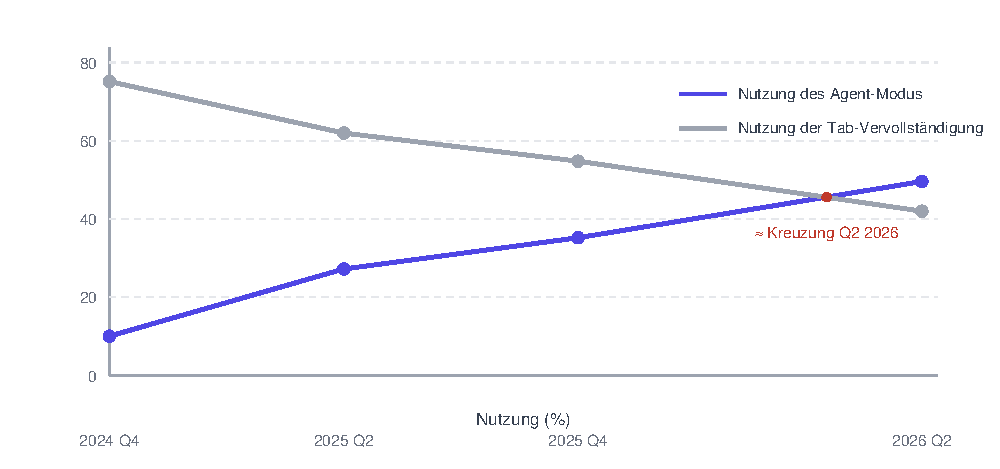
\includegraphics[width=0.92\linewidth]{figures/fig-di-san-shi-qi-zhang-1}
\\[2pt]\small Abbildung 1: Nutzung der Interaktionsmodi in der KI-Programmierung (Schätzung aus Branchendaten; Q2 2026 überholt Agent-Modus die Tab-Vervollständigung)
\end{center}

Ehrlich gesagt: Werkzeuge und Modelle sind nur Oberfläche. Ob Cursor oder Claude Code, ob GPT-5 oder Claude 4.5 – erfolgreiche Praktiker folgen derselben Grundmethodik. Genau die lehrt dieser Leitfaden.

\booksection{Der Kernwandel: Vom Coder zum Conductor}

Klassische Programmierlehre macht Sie zum Coder – Syntax verstehen, APIs lernen, Logikfehler debuggen. Im Zeitalter der KI-Programmierung wird die Rolle neu definiert: Sie müssen nicht mehr jede Zeile schreiben, aber zum „Dirigenten“ (Conductor) werden: Schlachtfeld definieren, Regeln setzen, Aufgaben verteilen, Ergebnisse abnehmen.

Der Kern liegt nicht darin, ob Sie Code schreiben können, sondern ob Sie klar denken können, was zu tun ist. Ein guter Dirigent ist nicht unbedingt der beste Soldat, kennt aber Ziel, Gelände und Truppenstärke am besten. So muss ein guter KI-Programmierer nicht jede Syntaxdetails beherrschen, aber Ziele, Architektur und Qualitätsmaßstäbe des Projekts genau kennen.

Diese Tabelle lohnt einen zweiten Blick – sie fasst den Rollenwandel zusammen:

\begin{center}
\begin{tabularx}{\linewidth}{|X|X|X|}
\hline
\textbf{Dimension} & \textbf{Klassischer Coder} & \textbf{KI-Dirigent (Conductor)} \tabularnewline
\hline
Kernkompetenz & Syntax, API-Aufrufe, Debugging & Anforderungen definieren, Kontext steuern, Abnahme \tabularnewline
Arbeitsweise & Zeile für Zeile schreiben & Absicht beschreiben, Ergebnisse prüfen \tabularnewline
Qualitätssicherung & Selbst geschrieben, selbst im Blick & KI-Ergebnisse durch Tests und Reviews prüfen \tabularnewline
Wissen & Tiefe Beherrschung einer Sprache/eines Frameworks & Breites Technikverständnis, tiefes Verständnis der Fachlogik \tabularnewline
Engpass & Tippgeschwindigkeit und Syntaxgedächtnis & Klarheit des Denkens und Ausdrucksvermögen \tabularnewline
Fehlerquellen & Syntaxfehler, logische Lücken & Unklare Anforderungen, fehlender Kontext \tabularnewline
\hline
\end{tabularx}
\end{center}

\begin{center}\small\color{gray}Klassischer Coder vs. KI-Dirigent im Vergleich\end{center}

Damit ist nicht gesagt, dass Programmierwissen unwichtig wäre. Ganz im Gegenteil: Wer KI-Code lesen kann, kann ihn wirksam prüfen und korrigieren; wer Datenstrukturen und Algorithmen versteht, kann die Pläne der KI bewerten. Wissen bestimmt die „Leitungsgrenze“ – aber seine Rolle wechselt vom Ausführungswerkzeug zum Urteilskriterium.

\booksection{Warum Methodik wichtiger ist als Werkzeuge}

Tools iterieren alle drei Monate, Methoden entwickeln sich erst alle drei Jahre weiter. Die Bedienung eines Tools kann nach drei Monaten veraltet sein; ein Denkansatz hält drei Jahre später noch.

Viele fragen beim Einstieg zuerst: „Welches Werkzeug ist am besten?“, „Welches Modell ist am stärksten?“ Wichtige Fragen, aber falsch priorisiert. Die Tool-Landschaft von August 2026 ist eine andere als August 2025 – Trae, Qoder und andere kommen und gehen, Cursor wurde vom Plugin zur eigenständigen IDE und dann zu Cursor 3, Claude Code vom Experiment zum Terminal-Standard. Doch hinter der Umtriebigkeit blieben die Denkprinzipien der Erfolgreichen fast unverändert.

Deshalb verschwendet dieses Buch keinen Platz für Bedienungsanleitungen einzelner Tools – die veralten im Handumdrehen. Stattdessen liegt der Fokus auf einer erprobten Denkmethodik: Anforderungen denken, mit der KI kommunizieren, Ergebnisse prüfen, iterativ verbessern. Wer diese Methodik beherrscht, kommt mit jedem Werkzeug schnell zurecht; wer nur Bedienung lernt, beginnt beim Toolwechsel bei null.

\begin{tcbinfo}{Beruhigung für Anfänger}
Wenn Sie neu einsteigen, lassen Sie sich vom Wort „Methodik“ nicht einschüchtern. Methodik ist keine abstrakte Philosophie, sondern ein Handbuch fürs Denken bei Problemen. Wie beim Kochen: Sie können einem Rezept folgen (Werkzeugbedienung), aber ein guter Koch versteht, „warum so würzen“ und „wie die Hitze steuern“ (Methodik). Dieses Buch erklärt die Grundlagen, jedes Prinzip mit konkreten Gegenbeispielen – damit Sie nicht nur verstehen, was gemeint ist, sondern wissen, wie es geht.

\end{tcbinfo}

\begin{tcbpractice}{Übung: Ihr persönliches „Rollenfoto“}
Nehmen Sie ein Blatt und beantworten Sie drei Fragen: (1) Wie nutzen Sie bisher KI beim Programmieren (falls überhaupt)? (2) Ähneln Sie eher dem „Coder“ oder dem „Dirigenten“ aus der Tabelle? (3) Wie würden Sie Ihre Arbeitsweise in drei Monaten beschreiben? Legen Sie den Zettel ins Buch und schauen Sie nach Kapitel 47 noch einmal herein – die Veränderung geht schneller, als Sie denken.

\end{tcbpractice}

\begin{tcbsummary}{Kapitel-Zusammenfassung}
\begin{itemize}
  \item 2025 nannte Karpathy die KI-Programmier-Revolution „Vibe Coding“: nicht Zeile für Zeile, sondern Absichten in natürlicher Sprache
  \item 2026 Weiterentwicklung zu Agentic Engineering: Ziel setzen, freigeben, KI plant und handelt, Mensch nimmt ab
  \item In Cursor 3 überholt der Agent-Modus erstmals die Tab-Vervollständigung; Claude Code bei 2,5 Mrd. USD Jahresumsatz
  \item Ihre neue Rolle: Conductor – Schlachtfeld definieren, Regeln setzen, Aufgaben verteilen, Ergebnisse abnehmen
  \item Werkzeuge entwickeln sich alle drei Monate, Methodik nur alle drei Jahre – Methodik lernen statt Bedienung
\end{itemize}

\end{tcbsummary}

\bookchapter{Kapitel 38: Fünf Denkprinzipien der KI-Programmierung}

\chapterintro{Wenn Sie aus diesem Buch nur ein Kapitel behalten, dann dieses. Die fünf Denkprinzipien sind sein Herzstück; alle späteren Kapitel – Kontext, Anforderungen, Dialog, Qualität – entfalten sie für verschiedene Situationen. Keines ist schwer zu verstehen, doch jedes lohnt sich, in einigen Projekten „in den Muskeln“ zu verankern.}

Der Ursprung ist spannend: Andrej Karpathy veröffentlichte zu seinem Open-Source-Projekt eine nur 70 Zeilen lange CLAUDE.md mit vier Kernprinzipien für die Zusammenarbeit mit KI. Die Datei erhielt auf GitHub über 70.000 Stars und wurde zur meistzitierten Richtschnur der KI-Programmierer weltweit. Es sind keine leeren Slogans, sondern aus der Praxis destillierte Denkgewohnheiten. Dieses Buch ergänzt die fünfte – iterative Verifikation – und vollendet so das System der fünf Prinzipien.

\begin{tcbinfo}{Warum ist eine 70-Zeilen-Datei so viel wert?}
Was bedeuten 70.000 Stars? Die meisten GitHub-Projekte erreichen das nie. Dass eine 70-Zeilen-Datei es schafft, zeigt: Im KI-Zeitalter ist nicht Code knapp, sondern die Fähigkeit, klar zu denken. Diese 70 Zeilen sind die destillierte Form dieses „Klar-Denkens“.

\end{tcbinfo}

\booksection{Prinzip 1: Think Before Coding (erst denken, dann kodieren)}

Das kontraintuitivste der fünf Prinzipien. Wenn KI uns beim Programmieren hilft, warum noch „erst denken“? Ganz einfach: Die Qualität der KI-Ausgabe hängt von Ihrer Eingabe ab. Wenn Sie selbst nicht wissen, was Sie wollen, geraten Sie in endlose „Änderungsschleifen“ – im Volksmund „KI irrt gemeinsam mit Ihnen“.

„Erst denken“ heißt: Vor der Anweisung an die KI drei Fragen klären – ein „Denk-Dreieck“, das vollständig sein muss:

\begin{enumerate}
  \item Welches Problem löse ich? (Ziel)
  \item Wie soll das Ergebnis aussehen? (Abnahmekriterien)
  \item Welche Einschränkungen gibt es? (Rahmen)
\end{enumerate}

\begin{center}
\begin{tabularx}{\linewidth}{|X|X|X|}
\hline
\textbf{Denkdimension} & \textbf{Unklare Eingabe (schlecht)} & \textbf{Klare Eingabe (gut)} \tabularnewline
\hline
Problemdefinition & Mach mir eine Website & Baue eine persönliche Tool-Seite mit drei Einstiegskarten für KI-Miniprogramme \tabularnewline
Erwartetes Ergebnis & Sieht gut aus & Responsives Layout, Dark Theme, Hover-Animationen auf den Karten, mobil nutzbar \tabularnewline
Einschränkungen & (nicht genannt) & Keine Frameworks, reines HTML+CSS+JS, Einzeldatei-Deployment, kein Backend \tabularnewline
\hline
\end{tabularx}
\end{center}

\begin{center}\small\color{gray}Unklare vs. klare Eingabe für dieselbe Anforderung\end{center}

\begin{tcbwarn}{Hinweis: „Erst denken“ $\neq$ „perfektes Dokument schreiben“}
„Erst denken“ heißt nicht „zuerst ein perfektes PRD schreiben“. Es ist ein schnelles, aber strukturiertes Denken – 30 Sekunden für die drei Fragen bringen mehr als 30 Minuten hin- und herändern im Chat. Bei kleinen Aufgaben genügt ein kurzer Dreiklang; bei großen Projekten wird daraus ein vollständiges Anforderungsdokument (siehe Kapitel 40).

\end{tcbwarn}

\booksection{Prinzip 2: Simplicity First (Einfachheit zuerst)}

Die größte Falle ist nicht „schafft es nicht“, sondern „macht zu viel“. Sagen Sie „Baue ein Benutzerverwaltungssystem“, generiert die KI oft Authentifizierung, Rechte, Rollen, Audit-Logs, Datenexport – obwohl Sie vielleicht nur eine einfache Login-Seite brauchen. Überproduktion ist die Hauptursache für aufgeblähten KI-Code.

„Einfachheit zuerst“ bedeutet „minimaler Machbarkeitsgrundsatz“: Mit dem wenigsten Code die Kernfunktion, mit der einfachsten Lösung das Problem, mit den wenigsten Features die Idee prüfen. Karpathy hat dafür ein treffendes Bild: „Wenn du nur einen Rabattpreis berechnen willst, brauchst du keinen E-Commerce-Motor.“

In der Praxis heißt das konkrete Gewohnheiten:

\begin{itemize}
  \item Pro Anweisung nur einen Funktionspunkt umsetzen, nicht das ganze System auf einmal;
  \item Standardbibliotheken und einfache Lösungen vor komplexen Abhängigkeiten;
  \item Was in 50 Zeilen geht, nicht auf 500 Zeilen aufblasen;
  \item Wenn die KI über das Ziel hinausschießt, klar sagen: „Überflüssiges streichen.“
\end{itemize}

\begin{center}
\begin{tabularx}{\linewidth}{|X|X|X|}
\hline
\textbf{Szenario} & \textbf{Überdimensionierte Lösung (vermeiden)} & \textbf{Einfache Lösung (empfohlen)} \tabularnewline
\hline
Daten speichern & MySQL-Datenbank + ORM aufsetzen & Erst JSON-Datei oder SQLite \tabularnewline
Benutzer-Login & OAuth2.0 + JWT + Rollenrechte & Erst einfache Passwortprüfung \tabularnewline
Frontend-Framework nötig & React + Redux + Router & Erst reines HTML + natives JS \tabularnewline
Deployment ins Netz & Docker + CI/CD + K8s & Erst lokal zum Laufen bringen \tabularnewline
\hline
\end{tabularx}
\end{center}

\begin{center}\small\color{gray}Überdimensionierte vs. einfache Lösungen in typischen Szenarien\end{center}

\booksection{Prinzip 3: Surgical Changes (chirurgisch präzise Änderungen)}

Beim Iterieren eines bestehenden Projekts sollte jede Änderung präzise sein wie eine Operation – nur das Nötige anfassen. Besonders wichtig in der KI-Programmierung, weil KI zum „Nebenbei-Mitändern“ neigt: Ein Bugfix wird leicht zur halben Datei-Refactorierung.

Kernanforderung: Jede Anweisung nennt explizit Umfang und Grenzen. „Ändere nur die Funktion calculate\_discount“, „Lass den Rest unangetastet“, „Behalte den vorhandenen Code-Stil“. Geht die Änderung darüber hinaus, sofort die überflüssigen Teile zurückverlangen.

Karpathy illustriert das mit einem Diff-Beispiel: Sie lassen eine „Mitgliedspreis“-Logik in die Rabattfunktion des Warenkorbs einbauen. Gutes Ergebnis: nur diese Funktion, wenige zusätzliche Zeilen. Schlechtes Ergebnis: der ganze File wird umgebaut – der neue Code mag „eleganter“ wirken, aber Sie wissen nicht, ob neue Bugs darin stecken. „Sieht besser aus“ darf in der KI-Programmierung nie ein Grund sein, von der Anweisung abzuweichen.

Schlechte Anweisung (unklarer Umfang)

\begin{lstlisting}
Optimiere die Rabattlogik dieses Projekts
\end{lstlisting}

Gute Anweisung (präziser Umfang)

\begin{lstlisting}
Ändere nur calculate\_discount in cart.py: 1. Ergänze Mitgliedspreis-Logik zur bestehenden Rabattlogik 2. Mitglieder erhalten zusätzlich 10 \% Rabatt 3. Funktionsparameter und andere Funktionen unverändert lassen 4. Vorhandenen Variablennamen-Stil beibehalten
\end{lstlisting}

\booksection{Prinzip 4: Goal-Driven Execution (zielgetriebene Ausführung)}

Diese Regel beantwortet eine Schlüsselfrage: Soll man der KI sagen, „wie“ sie arbeiten soll, oder „was“ herauskommen soll? Karpathys Antwort: das Letztere. Statt „Erst eine Klasse anlegen, dann Methoden, dann Tests“ besser: „Ich brauche ein Werkzeug, das CSV-Dateien einliest und je Spalte die Anzahl eindeutiger Werte zählt“. Die KI wählt den Weg, Sie nehmen das Ergebnis ab.

Der Vorteil ist doppelt: Die KI bekommt mehr Spielraum und wählt den besten Weg statt an Ihren Zwischenschritten zu kleben; Sie verlagern die Aufmerksamkeit vom „Wie“ auf „Ist es richtig?“ – genau das ist die Aufgabe eines Dirigenten.

\begin{tcbwarn}{Hinweis: Zielgetrieben $\neq$ gewähren lassen}
Nach der Ausführung muss streng abgenommen werden: Erfüllt das Ergebnis die Anforderung? Sind Randfälle behandelt? Gibt es Überdesign? Bei Abweichung konkretes Feedback geben – nicht „schreib neu“, sondern „Bei leerer Liste entsteht ein IndexError in Zeile 15, bitte eine Leerwertprüfung ergänzen“.

\end{tcbwarn}

\begin{center}
\begin{tabularx}{\linewidth}{|X|X|X|}
\hline
\textbf{Anweisungsstil} & \textbf{Beispiel} & \textbf{Ergebnismerkmal} \tabularnewline
\hline
Imperativ (wie) & „Lege eine Python-Klasse DataParser an, füge eine Methode parse mit Parameter filename hinzu, lese mit dem csv-Modul …“ & KI wird zur Tippkraft, Ihre Zwischenschritte sind vielleicht nicht optimal \tabularnewline
Zielorientiert (was) & „Ich brauche ein Tool: CSV einlesen, je Spalte eindeutige Werte zählen, als JSON ausgeben. Bitte vollständige Implementierung.“ & KI wählt den besten Weg, Sie prüfen das Ergebnis \tabularnewline
\hline
\end{tabularx}
\end{center}

\begin{center}\small\color{gray}Imperative vs. zielorientierte Anweisungen\end{center}

\booksection{Prinzip 5: Iterate and Verify (iterieren und prüfen)}

Dieses Buch ergänzt Karpathys vier Prinzipien um ein fünftes. Kernüberzeugung: Die erste KI-Ausgabe ist fast nie die Endversion. Effektive KI-Programmierung ist ein Kreislauf aus „Erzeugen – Prüfen – Korrigieren“, nicht ein einmaliges „Anweisung – Ergebnis“.

„Iterieren und prüfen“ ist nicht passives „Falsch, nochmal“, sondern ein strukturierter Verifikationsprozess. Nach jeder Ausgabe auf drei Ebenen prüfen:

\begin{itemize}
  \item Ebene 1 · Funktion: Läuft es? Sind Ein- und Ausgabe korrekt?
  \item Ebene 2 · Ränder: Was passiert bei leerer, zu langer oder fehlerhafter Eingabe?
  \item Ebene 3 · Architektur: Ist die Code-Struktur sinnvoll? Gibt es Hardcoding? Ist sie erweiterbar?
\end{itemize}

Ziel definieren

KI generiert Code

Funktionsprüfung

Bestanden

Grenzfälle prüfen

Bestanden

Architektur-Review

Bestanden, weiter zum nächsten Schritt

Nicht bestanden

Konkretes Feedback geben

Neu generieren

\begin{center}\small\color{gray}Abbildung 2: Iterativer Verifikationskreislauf der KI-Programmierung\end{center}

Der Schlüssel liegt im „konkreten Feedback“. Bei einem Fehlschlag nicht „stimmt nicht, mach neu“, sondern „Bei leerer Liste gibt es einen IndexError, bitte Zeile 15 um eine Leerwertprüfung ergänzen“. Präzises Feedback erlaubt gezielte Korrekturen; vages Feedback lässt die KI nur raten.

\booksection{Harness Engineering: Agent = Modell + Harness}

Mitte 2026 machte der Begriff Harness Engineering in der KI-Programmier-Community die Runde. Die Formel ist einfach:

Agent-Fähigkeit = Modellfähigkeit × Harness-Qualität

Die Modellfähigkeit ist die geistige Obergrenze; das Harness ist die „Arbeitsumgebung“ um das Modell – Kontextmanagement, Werkzeuganbindung, Prozesssteuerung, Gedächtnis.

Das erklärt ein häufiges Rätsel: Warum machen manche mit GPT-4 oder Claude brillante Projekte, andere nur mittelmäßigen Code? Der Unterschied liegt nicht im Modell, sondern im Harness. Ein gutes Harness umfasst klare Projektspezifikationen, sinnvolle Werkzeuge, geordneten Gesprächskontext und einen guten Verifikationsprozess. Das Modell setzt die Obergrenze, das Harness bestimmt, wie weit Sie sie ausschöpfen.

\begin{tcbinfo}{Das Praktikanten-Gleichnis}
Stellen Sie das Modell wie ein geniales Praktikanten vor – hoher IQ, aber ohne Projekthintergrund, Werkzeuge, Fristen und Abnahmekriterien kommt nichts Gutes heraus. Harness Engineering ist die Kunst, diesem Praktikanten die richtige Arbeitsumgebung zu bauen.

\end{tcbinfo}

Die folgenden Kapitel lehren genau das: Kapitel 39 Kontextmanagement (Projektgedächtnis), Kapitel 40 Anforderungen (PRD), Kapitel 43 Dialogtechnik (Prompt-Schichten), Kapitel 45 Qualitätssicherung (Verifikationsprozess). Zusammen ergeben sie Ihr Harness.

\begin{tcbpractice}{Übung: Die nächste Idee mit dem „Denk-Dreieck“ zerlegen}
Wählen Sie eine kleine Sache, die Sie schon lange machen wollten (z. B. eine Countdown-Seite, ein Trink-Erinnerungs-Skript). Drei Minuten lang beantworten: (1) Welches Problem löst es? (2) Wie sieht das Ergebnis aus? (3) Welche Rahmenbedingungen (Zeit, Technik, Umgebung)? Schreiben Sie die Antwort als einen Absatz. Glückwunsch – Ihr erstes „Think Before Coding“ ist fertig, und der Absatz ist eine brauchbare, hochwertige Anweisung.

\end{tcbpractice}

\begin{tcbsummary}{Kapitel-Zusammenfassung}
\begin{itemize}
  \item Die fünf Prinzipien stammen aus Karpathys 70-zeiliger CLAUDE.md (70K+ Stars); dieses Buch ergänzt „Iterate and Verify“
  \item Think Before Coding: Vor dem Sprechen drei Fragen – Was? Wie sieht es aus? Welche Grenzen?
  \item Simplicity First: Die größte Falle ist „zu viel“ – für einen Rabatt braucht man keinen Shop-Motor
  \item Surgical Changes: Chirurgisch präzise, kein „Nebenbei-Mitändern“ der KI
  \item Goal-Driven Execution: „Was“ statt „Wie“ – die KI wählt den Weg
  \item Iterate and Verify: Drei Prüfebene (Funktion/Rand/Architektur) + konkretes Feedback, im Kreislauf
  \item Harness Engineering: Fähigkeit = Modell × Harness – KI wie ein geniales Praktikanten führen
\end{itemize}

\end{tcbsummary}

\bookchapter{Kapitel 39: Kontextengineering – damit KI Ihre Absicht versteht}

\chapterintro{Kennst Sie das: Ein neues Chat-Fenster, und die KI scheint alles vergessen zu haben? Das ist keine Böswilligkeit, sondern „Vergesslichkeit“ von Natur aus. Dieses Kapitel zeigt, wie man der KI ein „Langzeitgedächtnis“ verpasst – und stellt eine der angesagtesten Entwicklungsparadigmen 2026 vor: spec-driven development.}

\booksection{Projektgedächtnisdatei: Das „Langzeitgedächtnis“ der KI}

Ein grundlegendes Limit: Das Gedächtnis der Modelle ist kurzlebig. Zu Beginn jeder Konversation kennt die KI Ihr Projekt nicht. Sie müssten immer wieder sagen: „Wir nutzen React“, „Backend ist Node.js“, „Datenbank PostgreSQL“, „Code-Stil mit doppelten Anführungszeichen“. Das ist mühsam und fehleranfällig – wie tägliches Onboarding für neue Kollegen.

Die Lösung: eine Projektgedächtnisdatei im Projektstamm. KI-Werkzeuge lesen sie automatisch beim Gesprächsstart. Die Benennung unterscheidet sich je Tool:

\begin{center}
\begin{tabularx}{\linewidth}{|X|X|}
\hline
\textbf{Werkzeug} & \textbf{Dateiname} \tabularnewline
\hline
Cursor & \texttt{.\allowbreak cursorrules} \tabularnewline
Claude Code & \texttt{CLAUDE.\allowbreak md} \tabularnewline
GitHub Copilot & \texttt{copilot-\allowbreak instructions.\allowbreak md} \tabularnewline
Allgemeine Lösung & \texttt{AGENTS.\allowbreak md} \tabularnewline
\hline
\end{tabularx}
\end{center}

\begin{center}\small\color{gray}Benennungskonventionen für Projektgedächtnisdateien\end{center}

Andere Namen, gleiche Idee: Alles, was die KI „immer wissen“ soll, gehört in diese Datei. Eine gute Projektgedächtnisdatei enthält: Projektüberblick, Technikstack, Code-Konventionen (Namensgebung, Einrückung, Kommentare), Verzeichnisstruktur, Entwicklungsabreden (Branch-Strategie, Commit-Regeln, Testanforderungen). Karpathys CLAUDE.md umfasst nur 70 Zeilen, deckt aber alle Schlüsselinfos ab – knapp und vollständig.

\begin{lstlisting}
# Projekt: App zur Verwaltung persönlicher Ausgaben
## Überblick
Eine Full-Stack-App zur Verwaltung persönlicher Ausgaben, mit der der Nutzer Einnahmen und Ausgaben des Alltags festhält.
## Tech-Stack
- Frontend: React + TypeScript + Tailwind CSS
- Backend: Node.js + Express + TypeScript
- Datenbank: SQLite (Entwicklung) / PostgreSQL (Produktion)
- Tests: Vitest
## Code-Konventionen
- Doppelte Anführungszeichen verwenden
- Einrückung mit 2 Leerzeichen
- Funktionsnamen in camelCase
- Typdefinitionen in PascalCase
- Jede Funktion braucht einen JSDoc-Kommentar
## Verzeichnisstruktur
/src
  /frontend  - Frontend-Code
  /backend   - Backend-Code
  /shared    - gemeinsame Typen für Frontend/Backend
  /tests     - Testdateien
## Entwicklungskonventionen
- Commit-Meldungen auf Deutsch
- Neue Funktionen immer zuerst mit Test
- API-Antworten durchgängig im Format { success, data, error }
\end{lstlisting}

\begin{tcbwarn}{Hinweis: Nicht zur „zweiten Anforderungsdoku“ verkommen lassen}
Achten Sie auf die Länge – keine Dutzende von Seiten. Ziel ist, der KI schnell Hintergrund zu geben, nicht jedes Feature auszuführen. Klar, strukturiert, nur das Nötige.

\end{tcbwarn}

\booksection{Spec-Driven Development (SDD)}

Spec-Driven Development (SDD) ist ein reifendes Paradigma 2026, Kernsatz: Erst Spezifikation, dann Code. Anders als klassisches TDD umfasst die „Spec“ nicht nur Tests, sondern auch Anforderungen, Schnittstellen und Datenmodelle. Die KI generiert Code daraus, Menschen schreiben und pflegen die Spezifikation.

Der SDD-Ablauf in fünf Schritten:

\begin{enumerate}
  \item Anforderungen in natürlicher Sprache beschreiben (als .md-Datei);
  \item Schnittstellen und Datenstrukturen festlegen (in der Spec-Datei);
  \item KI generiert die Implementierung nach Spec;
  \item Tests prüfen, ob das Ergebnis zur Spec passt;
  \item Falls nicht: Spec korrigieren oder KI den Code nachbessern lassen.
\end{enumerate}

In diesem Ablauf ist die Spec-Datei die „einzige Wahrheitsquelle“ – Code lässt sich neu erzeugen, die Spec muss stimmen.

Spezifikationsdokument schreiben

Ist die Spezifikation vollständig?

Vollständig

KI generiert Code nach der Spezifikation

Tests laufen lassen, um das Ergebnis zu prüfen

Unvollständig / Tests schlagen fehl

Code-Problem Code korrigieren; Spezifikationsproblem Spezifikation korrigieren

Zurück zur Prüfung

Alles bestanden Auslieferung

\begin{center}\small\color{gray}Abbildung 3: Arbeitsablauf von Spec-Driven Development (SDD)\end{center}

Vorteil: Spezifikationen sind stabiler als Code. Wechseln Modell oder Werkzeug, bleibt Ihre Spec gültig – der neue Generator setzt sie um. Deshalb betont dieses Buch „Methodik vor Werkzeug“: Die Spec-Datei ist der konkrete Träger Ihrer Methodik.

\booksection{Kontextfenster verwalten}

Selbst mit Projektgedächtnis stößt man im Gespräch an Grenzen des Kontextfensters (der gleichzeitig verarbeitbaren Informationsmenge). Bei zu langen Dialogen und vielen Dateien „vergisst“ die KI frühere Inhalte, die Qualität sinkt – wie nach sechs Stunden Plaudern mit einem Freund, der den ersten Satz längst vergessen hat.

Kernstrategie: „geschichtetes Zitieren“:

\begin{center}
\begin{tabularx}{\linewidth}{|X|X|X|}
\hline
\textbf{Kontextebene} & \textbf{Inhalt} & \textbf{Handhabung} \tabularnewline
\hline
Ebene 1: Projektgedächtnis & Technikstack, Konventionen, Verzeichnisbaum & In CLAUDE.md o. Ä. ablegen, wird automatisch geladen, nicht wiederholen \tabularnewline
Ebene 2: Datei-Referenzen & Code-Dateien der aktuellen Aufgabe & Mit @ präzise referenzieren, nicht ganze Dateien in den Chat kleben \tabularnewline
Ebene 3: Gesprächsverlauf & Dialoghistorie der aktuellen Aufgabe & Nach Abschluss neuen Chat beginnen, um Kontext nicht aufzublähen \tabularnewline
Ebene 4: Sofortige Anweisung & Konkrete Anforderung dieses Schritts & Klar, knapp, zielgerichtet – keine langatmigen Umschweife \tabularnewline
\hline
\end{tabularx}
\end{center}

\begin{center}\small\color{gray}Geschichtete Verwaltung des Kontextfensters\end{center}

\booksection{Praxispunkte fürs Kontext-Engineering}

Kontext-Engineering ist keine einmalige Einstellung, sondern ein fortlaufender Optimierungsprozess. Hier ein paar Punkte, die sich in der Praxis immer wieder bewährt haben:

\begin{enumerate}
  \item Halte die Gedächtnisdatei beim Weiterentwickeln des Projekts aktuell. Wenn du eine neue Technik einführst oder die Architektur änderst, aktualisiere sofort die Gedächtnisdatei, statt es im Chat improvisiert zu erklären.
  \item Nutze @-Verweise statt alles einzufügen. Die meisten KI-Coding-Tools unterstützen die Syntax @file oder @folder; sie schiebt den Dateiinhalt im Hintergrund in den Kontext der KI – effizienter als manuelles Einfügen, ohne den Chat zu überladen.
  \item Halte die Chats „kurz und knackig“. Ein Chat behandelt nur eine Aufgabe oder ein Feature. Wenn er fertig ist, starte fürs Nächste einen neuen Chat. Lange Chats verbrauchen nicht nur das Kontextfenster, sie lenken die KI auch ab.
  \item Lass die KI Ergebnisse „sehen“, statt sie zu „beschreiben“. Bei einem Bug gibst du das Fehlerprotokoll direkt per @-Verweis an die KI weiter, statt in eigenen Worten zu erzählen, „da sei wohl irgendein Fehler“. Die Rohinformation nützt der KI deutlich mehr als deine Wiedergabe.
  \item Räume regelmäßig auf und archiviere. Abgeschlossene Chats und temporäre Dateien belegen den Arbeitsbereich. Regelmäßiges Aufräumen hält das Projektverzeichnis sauber und hilft der KI, die Projektstruktur schneller zu erfassen.
\end{enumerate}

\begin{tcbpractice}{Ausprobieren: Schreibe für dein Projekt eine 70-Zeilen-Gedächtnisdatei}
Such dir ein Projekt aus, an dem du gerade arbeitest (oder arbeiten willst), und schreibe eine CLAUDE.md: Projektüberblick (2–3 Sätze), Tech-Stack (auflisten), Code-Richtlinien (3–5 Punkte), Verzeichnisstruktur (als Baum skizzieren), Entwicklungskonventionen (2–3 Punkte). Halte dich unter 70 Zeilen – danach wirst du merken, dass du dein Projekt selbst viel klarer verstehst.

\end{tcbpractice}

\begin{tcbsummary}{Zusammenfassung des Kapitels}
\begin{itemize}
  \item Das Gedächtnis der KI ist „kurzzeitig“: Bei jedem neuen Chat weiß sie null über dein Projekt
  \item Projekt-Gedächtnisdateien (CLAUDE.md \& Co.) sind das „Langzeitgedächtnis“ der KI und werden bei jedem Chat automatisch geladen
  \item Eine gute Gedächtnisdatei = Überblick + Tech-Stack + Richtlinien + Verzeichnis + Konventionen; 70 Zeilen genügen
  \item SDD, die spezifikationsgetriebene Entwicklung: erst die Spezifikation, dann der Code; die Spezifikation ist die „single source of truth“ und stabiler als der Code
  \item Kontext wird in vier Ebenen verwaltet: Projektgedächtnis @-Dateiverweise Chatverlauf direkte Anweisungen
  \item Fünf Praxispunkte: aktuell halten, @-Verweise, kurze Chats, Originalinfos geben, regelmäßig aufräumen
\end{itemize}

\end{tcbsummary}

\bookchapter{Kapitel 40: Anforderungsengineering – aus Ideen ausführbare Anweisungen für die KI machen}

\chapterintro{Während es beim Kontext-Engineering darum geht, dass die KI den Hintergrund versteht, sorgt das Anforderungsengineering dafür, dass die KI weiß, was diesmal konkret zu tun ist. Dieser Schritt zeigt beim KI-Programmieren am deutlichsten die Unterschiede zwischen Menschen: Mit denselben Tools und demselben Modell erschafft der eine verblüffende Projekte, der andere bringt nur mittelmäßiges Spielzeug zustande. Der Unterschied liegt selten im technischen Können – sondern darin, wie gut jemand Anforderungen formulieren kann.}

\booksection{Von der vagen Idee zur strukturierten Anforderung}

Jedes Projekt beginnt mit einer vagen Idee – „Ich will eine Haushaltsbuch-App bauen“, „Ich will eine private Website machen“, „Ich will ein Tool für To-do-Listen bauen“. Gegen die Ideen ist nichts einzuwenden – aber wirfst du sie direkt der KI hin, hängt die Qualität des Ergebnisses allein vom Glück ab. Ziel des Anforderungsengineerings ist es, diese vage Idee in eine strukturierte Anforderung zu verwandeln, die die KI präzise umsetzen kann.

Die gute Nachricht: Eine strukturierte Anforderung verlangt keinen PRD über zig Seiten. Du musst nur fünf Fragen beantworten – wir nennen sie die „fünf Anforderungselemente“:

\begin{center}
\begin{tabularx}{\linewidth}{|X|X|X|}
\hline
\textbf{Element} & \textbf{Frage} & \textbf{Beispiel: Haushaltsbuch-App} \tabularnewline
\hline
Who & Für wen ist es? & Persönliche Nutzung, um Einnahmen und Ausgaben des Alltags festzuhalten \tabularnewline
What & Was soll es tun? & Eine App, die jede Einnahme und Ausgabe erfasst, monatlich zusammenfasst und visualisiert \tabularnewline
Why & Warum baust du es? & Ich will meine Ausgabenstruktur verstehen und unnötige Kosten aufspüren \tabularnewline
How & Wie ungefähr? & Frontend mit React, Daten lokal im Browser speichern, Backend und Login erst einmal weglassen \tabularnewline
Constraint & Welche Einschränkungen gibt es? & Entwicklung allein, fertig in 2 Wochen, kein Livegang und Deployment nötig \tabularnewline
\hline
\end{tabularx}
\end{center}

\begin{center}\small\color{gray}Die fünf Anforderungselemente mit Beispielen\end{center}

Diese fünf Elemente musst du nicht als förmliches Dokument ausarbeiten – sie einmal zügig im Kopf durchzugehen genügt. Entscheidend ist die Gewohnheit, erst klar zu denken und dann loszulegen. Du wirst merken: Sobald du diese fünf Fragen klar beantworten kannst, wird deine Anforderungsbeschreibung ganz von selbst strukturiert.

\booksection{Die Kunst der gestuften Anforderungszerlegung}

Bei größeren Projekten reicht eine einzige Anforderungsbeschreibung nicht. Du musst die große Anforderung in kleine Teilanforderungen zerlegen, die sich einzeln überprüfen lassen. Das nennt man „Anforderungszerlegung“; der Grundsatz lautet: Jede Teilanforderung muss sich eigenständig umsetzen, eigenständig prüfen und eigenständig ausliefern lassen.

Am Beispiel „Eine private Haushaltsbuch-App bauen“ wäre eine sinnvolle Zerlegung:

\begin{enumerate}
  \item Die Grundfunktion zum Erfassen von Einnahmen und Ausgaben umsetzen (Einträge hinzufügen, ansehen, löschen);
  \item Kategorien ergänzen (jeden Eintrag mit Etiketten wie Essen, Verkehr und Co. versehen);
  \item Die monatliche Zusammenfassung umsetzen (Einnahmen und Ausgaben pro Monat auswerten);
  \item Datenvisualisierung ergänzen (die Ausgabenstruktur in Diagrammen zeigen).
\end{enumerate}

Jeder Schritt ist ein Funktions-Zuwachs, der sich eigenständig ausführen und prüfen lässt.

Goldene Regel zum Zerlegen von Anforderungen: Nach jedem Schritt muss das Projekt „etwas Benutzbares“ sein, so rudimentär auch. Lass das Projekt nie in dem Zustand „alles halb fertig und nichts benutzbar“ stecken.

Diese Zerlegung bringt zwei Vorteile. Erstens siehst du jederzeit Fortschritt – nach jedem Schritt kann deine App eine Funktion mehr; dieses positive Feedback ist bei Langzeitprojekten entscheidend (Erfolgserlebnisse brauchen wir alle). Zweitens bleibt jede einzelne Aufgabe für die KI klein genug, was das Risiko von „Verständnisabweichungen“ senkt – je kleiner die Aufgabe, desto genauer versteht die KI, desto besser das Ergebnis.

\booksection{PRD-Schreibvorlage und Praxis}

Bei größeren Projekten (etwa einer Full-Stack-App mit Front- und Backend und mehreren Funktionsmodulen) genügen die fünf Anforderungselemente womöglich nicht. Dann brauchst du ein förmlicheres Produktspezifikationsdokument (PRD). Ein oft missverstandener Punkt: Ein PRD ist nicht für die KI geschrieben – es ist für dich selbst, um deine Gedanken zu ordnen; erst danach kannst du der KI präzisere Anweisungen geben.

Ein gutes PRD muss nicht lang sein, sollte aber sechs Teile enthalten: Projektüberblick (in einem Absatz klären, worum es geht), Funktionsliste (was jeder Funktionspunkt ist), technischer Ansatz (welcher Tech-Stack, welche grobe Architektur), Datenmodell (die zentralen Datenstrukturen), Oberflächenbeschreibung (wie die wichtigsten Seiten aussehen) und Entwicklungsplan (in wie vielen Schritten es fertig wird).

\begin{lstlisting}
# PRD der Ausgaben-App
## Projektbeschreibung
Eine leichte Ausgaben-App: Einnahmen und Ausgaben erfassen, kategorisieren, Monatsübersichten und Datenvisualisierung.
## Funktionsliste
1. Buchung erfassen: Betrag, Typ (Einnahme/Ausgabe), Kategorie, Notiz, Datum
2. Kategorien: vordefiniert Essen, Verkehr, Einkäufe, Freizeit, Sonstiges
3. Monatsübersicht: Gesamteinnahmen, Gesamtausgaben und Saldo pro Monat
4. Ausgaben-Visualisierung: Kreisdiagramm mit Anteil je Kategorie
5. Datenexport: als CSV
## Technische Umsetzung
- Frontend: React + TypeScript + Tailwind CSS
- Speicherung: localStorage (ohne Backend)
- Diagramme: Chart.js
- Build: Vite
## Datenmodell
Record {
  id: string
  amount: number
  type: 'income' | 'expense'
  category: string
  note: string
  date: string  // YYYY-MM-DD
}
## Entwicklungsplan
Step 1: Grundfunktionen Buchungen (CRUD)
Step 2: Kategorienverwaltung
Step 3: Monatsübersicht
Step 4: Datenvisualisierung
Step 5: Datenexport
\end{lstlisting}

Achte auf den Schreibstil dieses PRD: knappe Listen und ein strukturiertes Format statt langer Ausführungen. Jeder Funktionspunkt ist klar definiert, das Datenmodell mit einfachen Typen beschrieben. Ein PRD in diesem Stil liest sich für dich selbst klar – und wenn du es der KI gibst, versteht sie jeden einzelnen Anforderungspunkt präzise.

\booksection{Praxis: die komplette Durchrechnung von der Idee zum Plan}

Reine Theorie ist langweilig – lass uns mit einem kompletten Beispiel den ganzen Weg des Anforderungsengineerings durchgehen. Nimm an, deine Idee lautet: „Ich will einen Lern-Tracker bauen, der festhält, was ich jeden Tag gelernt habe.“

Erster Schritt: die fünf Anforderungselemente durchgehen.

\begin{itemize}
  \item Who: Nur für mich selbst.
  \item What: Ein Tool, das festhält, was ich täglich lerne, meine Lernzeit verfolgt und den Lernfortschritt Revue passieren lässt.
  \item Why: Ich will mir eine dauerhafte Lerngewohnheit aneignen und meinen Zuwachs sehen.
  \item How: Erst eine Webversion, Daten lokal im Browser gespeichert.
  \item Constraint: Entwicklung ohne Vorkenntnisse, Kernfunktionen in 1 Woche fertig.
\end{itemize}

Zweiter Schritt: die Anforderungen zerlegen.

\begin{enumerate}
  \item Schritt 1: Die Funktion „Lerneintrag erfassen“ umsetzen (Datum, Inhalt, Dauer);
  \item Schritt 2: „Lernzeit-Statistik“ ergänzen (heute, Woche kumuliert);
  \item Schritt 3: Die Ansicht „Lernkalender“ umsetzen (angezeigt wie der GitHub-Beitragsgraph);
  \item Schritt 4: Die Funktion „Lernrückblick“ ergänzen (zeigt zufällig Einträge eines vergangenen Tages zum Wiederholen).
\end{enumerate}

Dritter Schritt: ein kurzes PRD schreiben. Es muss nicht lang sein – die Zerlegung oben bildet schon den Kern des PRD. Bring es in eine .md-Datei und lege sie ins Projektstammverzeichnis, als gemeinsame Referenz für dich und die KI.

Vierter Schritt: mit Schritt 1 der Entwicklung loslegen. Die Anweisung an die KI könnte lauten:

\begin{lstlisting}
Ich brauche die erste Funktion eines Lern-Trackers: Lerneinheiten erfassen.
Der Nutzer kann einen Eintrag mit Datum, Lerninhalt und Dauer (Minuten) hinzufügen.
Die Daten liegen in localStorage.
Frontend mit React + TypeScript.
Gib die vollständige Implementierung.
\end{lstlisting}

Beachte, was diese Anweisung auszeichnet: Sie beschreibt nur das Ziel des aktuellen Schritts (die Erfassungsfunktion), ohne andere Funktionen einzumischen; sie nennt die technischen Randbedingungen klar (React, TypeScript, localStorage); sie gibt genug Information, damit die KI weiß, „was“ zu tun ist und „wie“ vorzugehen ist, überlässt die konkrete Umsetzung aber der KI. Das ist eine hochwertige KI-Programmieranweisung, wie sie das Anforderungsengineering hervorbringt.

\begin{tcbpractice}{Ausprobieren: Schreibe für dein Herzensprojekt eine Fünf-Elemente-Karte}
Such dir ein kleines Projekt aus, das du schon lange mit dir herumträgst, und fülle in 5 Minuten eine Karte aus: Who / What / Why / How / Constraint – je ein Satz. Dann zerlege es in 3–5 Schritte, von denen jeder benutzbar ist. Du wirst merken: Einmal aufgeschrieben, wird aus dem „Tagtraum“ eine „To-do-Liste“.

\end{tcbpractice}

\begin{tcbsummary}{Zusammenfassung des Kapitels}
\begin{itemize}
  \item Die fünf Anforderungselemente: Who / What / Why / How / Constraint – erst klar denken, dann loslegen
  \item Goldene Regel der Anforderungszerlegung: Nach jedem Schritt ist das Projekt etwas „Benutzbares“
  \item Das PRD schreibst du für dich selbst: Überblick, Funktionsliste, technischer Ansatz, Datenmodell, Oberfläche, Plan
  \item Gute Anweisung = nur den aktuellen Schritt beschreiben + klare Randbedingungen + „was“ sagen, nicht „wie“
  \item Komplette Vorlage in vier Schritten: Fünf Elemente Zerlegung PRD Anweisung geben
\end{itemize}

\end{tcbsummary}

\bookchapter{Kapitel 41: Die KI-Coding-Tools 2026 im Überblick}

\chapterintro{Gleich eine Vorwarnung: Dieses Kapitel ist ein „Schnappschuss“ des Tool-Ökosystems vom August 2026. In einem halben Jahr ist er veraltet – und genau das ist die erste Lektion, die dich dieses Kapitel lehren will. Es geht nicht darum, dir zu zeigen, „welches Tool du benutzt“, sondern dir einen Beurteilungsrahmen dafür mitzugeben, „wie du Tools auswählst“. Wenn du die Design-Philosophie der verschiedenen Tools verstehst, triffst du jederzeit die Wahl, die zu dir passt.}

\booksection{Drei Schulen und der Auswahlrahmen}

Die KI-Coding-Tools von 2026 lassen sich grob in drei Schulen einteilen, hinter jeder steht eine eigene Design-Philosophie. Zuerst der Überblick:

\begin{center}
\begin{tabularx}{\linewidth}{|X|X|X|X|}
\hline
\textbf{Schule} & \textbf{Typische Tools} & \textbf{Design-Philosophie} & \textbf{Geeignet für} \tabularnewline
\hline
KI im IDE & Cursor 3, Trae, Windsurf, CodeBuddy & KI-Fähigkeiten tief in den Editor integrieren & Alltagsentwicklung, Code-Reviews, schrittweise Erweiterung \tabularnewline
Terminal-Agenten & Claude Code, Codex CLI, Aider & Das Terminal als Oberfläche; die KI bedient Dateisystem und Befehle direkt & Projektweite Aktionen, Massenänderungen, CI/CD-Integration \tabularnewline
Cloud-Builder & v0, Bolt, Replit Agent & Komplette Projekte im Browser von null aufbauen & Schnelle Prototypen, Einstieg ohne Konfiguration, sofortige Vorschau \tabularnewline
\hline
\end{tabularx}
\end{center}

\begin{center}\small\color{gray}Die drei Schulen der KI-Coding-Tools\end{center}

Bei der Toolwahl kommt es nicht darauf an, „welches am besten ist“, sondern darauf, „welches zu deiner aktuellen Situation passt“. Drei praktische Prüffragen:

\begin{itemize}
  \item Wie steht es um deine Programmiergrundlagen? Ganz ohne Vorkenntnisse: Cloud-Builder. Mit Grundlagen: KI im IDE. Fortgeschrittene: Terminal-Agenten.
  \item In welcher Phase steckt dein Projekt? Vom Nullpunkt starten: Cloud-Builder. Iterativ entwickeln: KI im IDE. Warten und Refactoring: Terminal-Agenten.
  \item Was brauchst du fürs Deployment? Schnell validieren: Cloud-Builder. Ernstzunehmende Projekte: KI im IDE. Automatisierte Abläufe: Terminal-Agenten.
\end{itemize}

\booksection{Die Schule „KI im IDE“}

KI im IDE ist die verbreitetste Schule: Die KI-Fähigkeiten werden in deinen Code-Editor eingebettet, sodass das klassische Programmiererlebnis erhalten bleibt und die KI-Erweiterung obendrauf kommt. Die Vertreter dieser Schule 2026 sind Cursor 3, Trae, Windsurf und CodeBuddy.

\booksubsection{Cursor 3}

Cursor ist derzeit das weltweit am weitesten verbreitete KI-Coding-IDE. Cursor 3, im April 2026 erschienen, markiert eine wichtige Wende bei den KI-Coding-Tools: Der Agent-Modus hat den Tab-Vervollständigungsmodus bei der Nutzung erstmals überholt – Entwickler wechseln von „die KI vervollständigt meinen Code“ zu „die KI erledigt meine Aufgabe“. Zu den Kernfunktionen von Cursor 3 gehören: Mehrdateien-Editing (die KI kann mehrere Dateien gleichzeitig ändern, um eine Aufgabe zu lösen), Kontextbewusstsein (versteht Projektstruktur und Abhängigkeiten automatisch) und die tiefe Terminal-Integration (die KI kann Befehle direkt im Editor ausführen und die Ausgaben ansehen).

\booksubsection{Trae}

Trae ist das KI-Coding-IDE von ByteDance mit einer großen Nutzerbasis auf dem chinesischen Markt. Sein SOLO-Modus (auch Builder-Modus) ist die typische „Projekt aus einem Satz“-Fähigkeit – du beschreibst die Anforderung, und die KI erledigt eigenständig den kompletten Weg von der Projektinitialisierung bis zur Codeerzeugung. Traes Stärken sind die chinesische Sprachunterstützung und die Anpassung an die Netzumgebung in China – ideal für Nutzer dort, um schnell einzusteigen.

\booksubsection{Weitere Tools}

Windsurf (früher Codeium) ist für sein flüssiges Code-Vervollständigungserlebnis bekannt – perfekt für Entwickler, die „tippen wie im Fluge“ wollen. Tencent Cloud CodeBuddy kommt als VS-Code-Plugin daher, ist stark in Cloud-Ökosysteme integriert und passt zu Projekten, die auf Tencent Cloud deployt werden oder WeChat-Miniprogramme entwickeln. Auch Alibaba Tongyi Lingma und Baidu Comate bieten ähnliche IDE-Integration, jeweils mit eigenen Stärken bei der Optimierung für chinesische Szenarien.

\booksection{Die Schule „Terminal-Agenten“}

Terminal-Agenten sind 2026 die am schnellsten wachsende Schule. Der Kerngedanke: Die KI sollte nicht bloß ein Editor-Plugin sein, sondern das ganze Entwicklungsumfeld wie ein Entwickler bedienen können – Dateien lesen und schreiben, Befehle ausführen, Ausgaben prüfen, Abhängigkeiten installieren. Claude Code ist der Vertreter dieser Schule.

\booksubsection{Claude Code}

Claude Code ist das Terminal-KI-Coding-Tool von Anthropic und hatte bis Mitte 2026 einen annualisierten Umsatz von 2,5 Milliarden US-Dollar erreicht. Die Arbeitsweise unterscheidet sich komplett von klassischen IDEs: Du beschreibst die Aufgabe im Terminal in natürlicher Sprache, und Claude Code liest eigenständig die relevanten Dateien, ändert den Code, führt Tests aus, prüft die Ergebnisse und iteriert nach – ohne dass du dafür den Editor öffnen musst.

Claude Codes Stärke ist das „Gesamtprojekt-Bewusstsein“: Es ist nicht auf ein Editorfenster beschränkt, kann frei durchs gesamte Projektverzeichnis browsen und die Abhängigkeiten zwischen Dateien verstehen. Es unterstützt auch die Projekt-Gedächtnisdatei CLAUDE.md, damit die KI bei jedem Sitzungsstart den Hintergrund kennt. Für Refactoring in großen Projekten, Massenänderungen oder das Schreiben von Tests sind Terminal-Agenten effizienter als IDE-Plugins.

\booksubsection{Codex CLI und Aider}

OpenAIs Codex CLI bietet ein ähnliches Terminal-Coding-Erlebnis und unterstützt die Funktion /import – damit lassen sich bestehende Codebasen importieren, damit die KI sie versteht. Aider ist ein Open-Source-KI-Coding-Tool fürs Terminal, das verschiedene Modelle unterstützt (GPT, Claude, DeepSeek und mehr) und sich für Nutzer eignet, die flexibel das Modell wechseln wollen. Diese Tools unterscheiden sich im Detail, teilen aber denselben Kerngedanken: Die KI soll im Terminal die volle Kontrolle über die Entwicklungsumgebung haben.

\booksection{Die Schule „Cloud-Builder“}

Cloud-Builder sind die Schule für Nutzer ohne jede Vorerfahrung. Du installierst keine Software, öffnest nur den Browser, beschreibst deine Anforderung – und die KI baut in der Cloud ein komplettes Projekt auf, mit sofortiger Vorschau.

\begin{itemize}
  \item v0 (von Vercel): stark beim Erzeugen von Frontend-UI-Komponenten und Seiten, ideal, um schnell Web-Prototypen zu bauen.
  \item Bolt: kann aus einem einzigen Satz eine Full-Stack-App erzeugen, inklusive Frontend, Backend und Datenbank.
  \item Replit Agent: arbeitet im Cloud-IDE von Replit und kann Projekte nicht nur anlegen, sondern sie direkt in der Cloud ausführen und deployen.
\end{itemize}

Der gemeinsame Vorteil dieser Tools ist der „Start ohne Konfiguration“ – Browser öffnen, loslegen. Die Grenze: Sobald das Projekt komplexer wird, ist die Cloud-Editierumgebung weniger flexibel als ein lokales IDE. Deshalb eignen sie sich am besten für die Prototypen-Phase „von 0 auf 1“: erst mit einem Cloud-Builder die Idee schnell prüfen, dann für die vertiefte Entwicklung in ein lokales IDE umziehen.

\booksection{Tools wechseln, die Methode bleibt}

Drei Gewohnheiten, die du behalten solltest, selbst wenn morgen alle KI-Programmier-Tools verschwinden: erst denken, dann handeln; immer nur einen kleinen Schritt; nach dem Tun verifizieren. Tools sind der Verstärker, die Methodik das Fundament. Den Verstärker kannst du tauschen, das Fundament darf nicht wackeln.

Blick zurück auf 2024 bis 2026: 2024 war GitHub Copilot der König, 2025 übernahm Cursor den Thron, 2026 stieg Claude Code überraschend auf. Immer wenn ein neues Tool erscheint, behaupten einige, „diesmal sei alles anders“ – am Ende zeigt sich: Wer neue Tools gut nutzt, sind genau die mit solider Methode. Sie brauchen beim Toolwechsel nur ein paar Tage Eingewöhnung; wer dagegen nur die Bedienung eines Tools gelernt hat, fängt bei jedem Wechsel von vorn an.

Deshalb lautet der Lernpfad, den dieses Buch empfiehlt: Steig erst mit einem Tool ein (egal welchem) und spüre in der Praxis die fünf Denkprinzipien; wenn deine Methode solide genug ist, probiere Tools aus anderen Schulen und erlebe den Unterschied ihrer Design-Philosophien; am Ende findest du zu deiner eigenen Toolkombination – etwa Cursor für die Alltagsentwicklung, Claude Code für Refactoring und Tests, v0 für schnelle Prototypen. Die Toolkombination ist bei jedem anders, die Methode aber gilt für alle.

\begin{tcbpractice}{Ausprobieren: Stell dein eigenes „Werkzeug-Arsenal“ zusammen}
Ordne dich mit den drei Prüffragen (Programmiergrundlagen, Projektphase, Deployment-Bedarf) ein: Ganz ohne Vorerfahrung probier Bolt oder v0 und bau eine Seite; mit Grundlagen mach mit Cursor oder Trae eine iterierende Aufgabe; als Herausforderung starte einmal Claude Code im Terminal. Beantworte dann: Welche Schule passt am besten zu deiner aktuellen Phase?

\end{tcbpractice}

\begin{tcbsummary}{Zusammenfassung des Kapitels}
\begin{itemize}
  \item Drei Schulen: KI im IDE (Alltagsentwicklung), Terminal-Agenten (projektweite Aktionen), Cloud-Builder (Prototypen ohne Vorkenntnisse)
  \item Toolwahl in drei Fragen: Programmiergrundlagen? Projektphase? Deployment-Bedarf?
  \item Cursor 3: Agent-Modus erstmals vor Tab-Vervollständigung; Claude Code: 2,5 Mrd. US\$ annualisierter Umsatz
  \item Cloud-Builder passen zu „von 0 auf 1“; nach der Validierung zurück ins lokale IDE für die vertiefte Entwicklung
  \item Tools iterieren alle drei Monate: Wer die Methode gelernt hat, braucht beim Wechsel nur wenige Tage Eingewöhnung
\end{itemize}

\end{tcbsummary}

\bookchapter{Kapitel 42: Das Panorama der großen Modelle und die API in der Praxis}

\chapterintro{Die letzten Kapitel haben sich damit beschäftigt, wie du mit der KI zusammenarbeitest. Dieses Kapitel beantwortet eine noch grundlegendere Frage: „Welche KI? Und wie benutze ich sie?“ Das große Modell-Panorama vom August 2026 ist ungeheuer vielfältig – international liefern sich GPT, Claude und Gemini ein Dreikampf, in China blühen DeepSeek, Tongyi Qianwen, GLM, Kimi und Doubao nebeneinander auf. Jedes Modell hat seinen eigenen Charakter und seine Stärken: Die richtige Wahl halbiert deine Mühe, die falsche verdoppelt sie. Dieses Kapitel stellt dir diese Modelle nicht nur vor, sondern zeigt dir auch, wie du sie über eine API in deine eigenen Apps einbindest und wie du passend zu deinem Bedarf den richtigen Token-Plan (Nutzungspaket) wählst.}

\booksection{Die internationalen Leitmodelle: drei starke Anbieter}

Auf dem internationalen Markt der großen Modelle haben sich im August 2026 drei starke Anbieter etabliert: OpenAI (GPT-Serie), Anthropic (Claude-Serie) und Google (Gemini-Serie). Jeder hat einen deutlich eigenen Charakter – lass uns sie einen nach dem anderen kennenlernen.

\booksubsection{Die OpenAI-GPT-5.6-Serie: der rundum ausbalancierte Allrounder}

OpenAI hat die Welle der großen Modelle ausgelöst, und die GPT-Serie ist bis heute das weltweit am häufigsten genutzte Modell. Die im Juli 2026 erschienene GPT-5.6-Serie folgt einer Drei-Stufen-Strategie: das Flaggschiff GPT-5.6 Sol für anspruchsvolle Inferenz, das ausgewogene GPT-5.6 Terra für die Alltagsentwicklung und das leichte GPT-5.6 Luna für Szenarien mit hohem Aufkommen und niedrigen Kosten. Alle drei Modelle teilen sich ein Kontextfenster von 1,05 Mio. Token und unterstützen Bildeingabe, Funktionsaufrufe und strukturierte Ausgaben.

\begin{center}
\begin{tabularx}{\linewidth}{|X|X|X|X|X|}
\hline
\textbf{Modell} & \textbf{Positionierung} & \textbf{Eingabe (/Mio. Token)} & \textbf{Ausgabe (/Mio. Token)} & \textbf{Kontextfenster} \tabularnewline
\hline
GPT-5.6 Sol & Flaggschiff-Inferenz & 5,00 US\$ (ca. 36 RMB) & 30,00 US\$ (ca. 217 RMB) & 1,05 Mio. Token \tabularnewline
GPT-5.6 Terra & ausgewogen, Alltag & 2,50 US\$ (ca. 18 RMB) & 15,00 US\$ (ca. 109 RMB) & 1,05 Mio. Token \tabularnewline
GPT-5.6 Luna & leicht, niedrige Kosten & 1,00 US\$ (ca. 7 RMB) & 6,00 US\$ (ca. 44 RMB) & 1,05 Mio. Token \tabularnewline
\hline
\end{tabularx}
\end{center}

\begin{center}\small\color{gray}Preisliste der OpenAI-GPT-5.6-Serie (August 2026)\end{center}

Die Kernstärke der GPT-Serie ist die Ausgewogenheit – Inferenz, Programmieren, Schreiben, Multimodalität: keine auffällige Schwäche. Dazu kommen OpenAIs riesiges Plugin-Ökosystem und Entwickler-Community; Dokumentation und Werkzeugkette sind am vollständigsten. Für Situationen, in denen du nicht weißt, was du wählen sollst, ist GPT die Standardantwort, die „blind gewählt“ nie falsch liegt. Die Schwächen: Der Zugriff von China aus erfordert spezielle Netzwerkwege, das Chinesische klingt gelegentlich nach „Übersetzerton“, und die API-Preise liegen im mittleren bis hohen Bereich.

\textbf{Gute Nachricht}\par

OpenAI kündigte im August 2026 an, dass das Standardmodell für Gratisnutzer auf GPT-5.6 Luna angehoben wurde und unbegrenzte Text-Chats freigeschaltet sind. Das heißt: Die Grundfähigkeiten von GPT erlebst du ohne Kosten; zahlen musst du erst, wenn du stärkere Inferenz oder API-Aufrufe brauchst.

\booksubsection{Die Anthropic-Claude-Serie: die Spitze beim Programmieren und bei der Sorgfalt}

Wenn GPT der Allrounder ist, dann ist Claude beim Programmieren die „Messlatte“. Anthropics Claude-Serie führt beim SWE-bench (Software-Engineering-Benchmark) seit Langem mit klarem Abstand; Codequalität und die Fähigkeit, Projekte in Ingenieursqualität umzusetzen, sind Branchenspitze. Noch bemerkenswerter: Claude hat die niedrigste Halluzinationsrate (Wahrscheinlichkeit falscher Angaben) im gesamten Feld, nur etwa 1 \% – dadurch eignet es sich besonders für präzisionskritische Bereiche wie Wissenschaft und Recht.

Claudes zweiter Trumpf ist der extrem lange Kontext: ein Kontextfenster von 1 Mio. Token, mit dem sich mehrhundertseitige Verträge oder ganze Codebasen in einem Zug „durchlesen“ lassen, ohne Details zu verlieren. Beim Code-Refactoring, bei der Analyse langer Dokumente und Ähnlichem ist das praktisch unersetzlich. Claude Code, das Terminal-KI-Coding-Tool, erreichte bis Mitte 2026 einen annualisierten Umsatz von 2,5 Milliarden US-Dollar – der deutlichste Beleg dafür, wie anerkannt Claudes Programmierfähigkeit ist.

\begin{center}
\begin{tabularx}{\linewidth}{|X|X|X|X|X|}
\hline
\textbf{Modell} & \textbf{Positionierung} & \textbf{Eingabe (/Mio. Token)} & \textbf{Ausgabe (/Mio. Token)} & \textbf{Kontextfenster} \tabularnewline
\hline
Claude Fable 5 & Flaggschiff & 10,00 US\$ (ca. 72 RMB) & 50,00 US\$ (ca. 362 RMB) & 1 Mio. Token \tabularnewline
Claude Opus 4.8 & Profi-Modell & 5,00 US\$ (ca. 36 RMB) & 25,00 US\$ (ca. 181 RMB) & 1 Mio. Token \tabularnewline
Claude Sonnet 5 & Preis-Leistungs-Modell & 2,00 US\$ (ca. 14 RMB) & 10,00 US\$ (ca. 72 RMB) & 1 Mio. Token \tabularnewline
\hline
\end{tabularx}
\end{center}

\begin{center}\small\color{gray}Preisliste der Anthropic-Claude-Serie (August 2026; Sonnet 5 zum Aktionspreis)\end{center}

Claudes Schwäche ist der Preis – Fable 5 hat mit 50 US\$ pro Mio. Token den höchsten Ausgabepreis aller Modelle. Die Multimodal-Fähigkeiten (Bild- und Videoverständnis) sind ebenfalls relativ schwach. Für Einzelentwickler mit kleinem Budget ist Sonnet 5 in der Aktionsphase preislich äußerst attraktiv.

\booksubsection{Die Google-Gemini-Serie: der König der Multimodalität}

Googles Gemini-Serie ist 2026 bis zur Version 3.1 Pro weiterentwickelt. Geminis größter Trumpf ist die native Multimodalität – präzises Auswerten von Text und Bildern, fehlerfreie OCR-Tabellenerkennung, effizientes Extrahieren von Videoframes, dazu tiefgehende Analyse von Audio und Video. Es ist fest mit dem Google-Ökosystem (Suche, Mail, Cloud-Dienste) verzahnt und glänzt bei Echtzeit-Informationssuche und übergreifendem Modalitäten-Verständnis. Gemini unterstützt zudem eine Eingabe von bis zu 2 Mio. Token Kontext – aktuell das größte Kontextfenster überhaupt.

Gemini positioniert sich als „erste Wahl für wissenschaftliche Inferenz und Multimodal-Szenarien“. Wenn dein Projekt viel Bildanalyse, Videoverständnis oder wissenschaftliche Berechnung umfasst, hat Gemini kaum Gegner. Beim reinen Text-Codegenerieren liegt es allerdings leicht hinter Claude, und seine chinesischen Formulierungen wirken nicht so natürlich wie die der chinesischen Modelle.

\begin{center}
\begin{tabularx}{\linewidth}{|X|X|X|X|}
\hline
\textbf{Vergleichspunkt} & \textbf{GPT-5.6} & \textbf{Claude Fable 5} & \textbf{Gemini 3.1 Pro} \tabularnewline
\hline
Gesamtwertung & 94.8 & 95.0 & 92.1 \tabularnewline
Programmierfähigkeit (SWE-bench) & 74.9\% & 64.3\% (Pro) & Mittel \tabularnewline
Kontextfenster & 1,05 Mio. Token & 1 Mio. Token & 2 Mio. Token \tabularnewline
Multimodal-Fähigkeiten & ausgewogen & schwächer & am stärksten \tabularnewline
Halluzinationsrate & niedrig & am niedrigsten (ca. 1 \%) & niedrig \tabularnewline
Verfügbarkeit in China & Sonderzugang nötig & Sonderzugang nötig & Sonderzugang nötig \tabularnewline
API-Ökosystem & am ausgereiftesten & im Aufbau & an das Google-Ökosystem gebunden \tabularnewline
\hline
\end{tabularx}
\end{center}

\begin{center}\small\color{gray}Die drei großen internationalen Modelle im Vergleich (August 2026)\end{center}

\begin{tcbwarn}{Achtung: die praktische Hürde bei der Nutzung in China}
Für Entwickler in China ist die zentrale Hürde bei GPT, Claude und Gemini der Netzwerkzugang. Zwar lässt sich indirekt über Azure-Proxys oder API-Aggregationsplattformen arbeiten, doch Stabilität und Regelkonformität musst du selbst abwägen. Wenn dein Projekt strenge Anforderungen an die Datensicherheit stellt, lohnt es sich, zuerst heimische Modelle in Betracht zu ziehen.

\end{tcbwarn}

\booksection{Die chinesischen Leitmodelle: eine blühende Vielfalt}

Die großen chinesischen Modelle sind 2026 vom „Verfolger“ zum „Gleichauf-Läufer“ geworden und in manchen Feldern sogar zur „Spitze“. Anders als 2023, als ihnen der Vorwurf gemacht wurde, sie setzten nur auf fremde Modelle auf, stehen die chinesischen Flaggschiffe 2026 bei logischer Inferenz, Codeerzeugung und Chinesisch-Verständnis auf Augenhöhe mit den internationalen Top-Modellen – der Abstand ist auf unter 5 \% geschrumpft. Wichtiger noch: Bei chinesischen Szenarien, Kosten und regelkonformer Bereitstellung bieten sie unersetzbare Vorteile.

\booksubsection{DeepSeek V4: der König des Preis-Leistungs-Verhältnisses}

DeepSeek ist eine Erscheinung für sich unter den chinesischen Modellen. Anfang 2025 erschütterte DeepSeek-V3 den Markt mit dem Profil „ein Zehntel des GPT-Preises bei vergleichbarer Leistung“; die Branche nannte es die „K.-o.-Schwelle der Allzweck-KI“ – billiger als DeepSeek ist nichts so gut, teurer bietet nicht so viel fürs Geld. Im August 2026 erschien die finale Version DeepSeek V4-Pro: 1,6 Billionen Parameter im MoE-Aufbau, rund 49 Milliarden davon aktiv, 1 Mio. Token verlustfreier Kontext; beim Preis-Leistungs-Verhältnis für Code gilt es vielfach als weltweite Spitze.

DeepSeek V4 springt bei den Agent-Fähigkeiten deutlich nach vorn – der DeepSWE-Benchmark steigt von 12,8 auf 62,7 (+390 \%), NL2Repo von 38,5 auf 61,5. Die API unterstützt jetzt sowohl das Responses-API- als auch das Anthropic-API-Protokoll und ist damit kompatibel mit gängigen Coding-Tools wie Codex und Claude Code. Das heißt: Du kannst in Claude Code die DeepSeek-API statt der Claude-API nutzen – ein Bruchteil der Kosten bei fast identischem Erlebnis.

\begin{center}
\begin{tabularx}{\linewidth}{|X|X|X|X|X|}
\hline
\textbf{Modell} & \textbf{Positionierung} & \textbf{Eingabe (/Mio. Token)} & \textbf{Ausgabe (/Mio. Token)} & \textbf{Kontextfenster} \tabularnewline
\hline
DeepSeek V4 Pro & Flaggschiff-Inferenz & 3 RMB (ca. 0,43 US\$) & 6 RMB (ca. 0,87 US\$) & 1 Mio. Token \tabularnewline
DeepSeek V4 Flash & leicht und schnell & 1 RMB (ca. 0,14 US\$) & 2 RMB (ca. 0,28 US\$) & 1 Mio. Token \tabularnewline
\hline
\end{tabularx}
\end{center}

\begin{center}\small\color{gray}Preisliste der DeepSeek-V4-Serie (August 2026, Aktionspreise)\end{center}

Preisvergleich: Für je 1 Mio. Token Eingabe plus 1 Mio. Token Ausgabe zahlst du bei DeepSeek V4 Flash rund 0,42 US\$, bei GPT-5.6 Sol rund 35 US\$ und bei Claude Fable 5 rund 60 US\$ – ein Unterschied von bis zu 80- bis 140-fach.

\textbf{Stolperfalle: DeepSeek wird teurer}\par

DeepSeek hat am 6. August 2026 offiziell angekündigt, „in Kürze die API-Preise deutlich anheben zu wollen“ – die Aktionspreise dürften also nicht mehr lange gelten. In einzelnen Medien war vom bis zu 30-fachen die Rede; bis zum 14. August lag der endgültige Preisplan aber noch nicht vor. Außerdem führt die finale Version von DeepSeek V4 eine Spitzen-/Talzeit-Preisgestaltung ein – in Stoßzeiten verdoppeln sich die Aufrufpreise. Achte auf die offiziellen Ankündigungen für die aktuellsten Preise.

\booksubsection{Tongyi Qianwen Qwen3.7 Max: Alibaba Clouds Wahl für Unternehmen}

Die Tongyi-Qianwen-Serie (Qwen) von Alibaba Cloud profitiert vom Alibaba-Cloud-Ökosystem und hat bei Enterprise-Deployments klare Vorteile. Das im Juli 2026 erschienene Qwen3.7 Max ist das aktuelle Flaggschiff: ein dichtes Modell mit 235B Parametern, 256K nativem Kontext, erweiterbar auf 1M. Qwens Kernstärken: ein ausgereiftes Open-Source-Ökosystem (die ganze Serie von 7B bis 235B ist offen), präzises Verständnis chinesischer Szenarien und tiefe Integration in die Alibaba-Cloud-Infrastruktur.

\begin{center}
\begin{tabularx}{\linewidth}{|X|X|X|}
\hline
\textbf{Modell} & \textbf{Ausgabepreis (/Mio. Token)} & \textbf{Geeignet für} \tabularnewline
\hline
qwen-turbo & 0,6 RMB & schlichte Frage-Antwort, Textklassifikation, hohes Aufkommen \tabularnewline
qwen-long & 2,0 RMB & Verarbeitung extrem langer Kontexte (10M) \tabularnewline
qwen3.7-flash & 7,2 RMB & allgemeine Chats, Inhaltserstellung \tabularnewline
qwen3.7-plus & 12,0 RMB & Multimodalität (Bild + Video), chinesisches Schreiben \tabularnewline
qwen3.7-max & 36,0 RMB & Flaggschiff für Chinesisch, komplexe Aufgaben \tabularnewline
\hline
\end{tabularx}
\end{center}

\begin{center}\small\color{gray}Staffelpreise der Tongyi-Qianwen-Serie Qwen (August 2026)\end{center}

Qwen staffelt seine Preise – vom extrem günstigen qwen-turbo (Ausgabe 0,6 RMB/Mio. Token) bis zum Flaggschiff qwen3.7-max (Ausgabe 36 RMB/Mio. Token) deckt die Serie alles ab, vom leichten Frage-Antwort-Betrieb bis zu komplexer Inferenz. Für Unternehmen, die ohnehin Alibaba Cloud nutzen, ist Qwen die naheliegendste Integrationswahl.

\booksubsection{Zhipu GLM-5.1: chinesische Nummer 1 beim SWE-bench}

Die GLM-Serie von Zhipu AI glänzt 2026. GLM-5.1 holte beim SWE-bench den ersten Platz unter den chinesischen Modellen: eine MoE-Architektur mit 744B Parametern und 1 Mio. Token Kontext. Es versteht chinesische Semantik präzise und erlaubt in China regelkonforme, lokale Bereitstellung (On-Premise) – entscheidend für Finanz- und Behördenszenarien mit hohen Datensicherheitsanforderungen. GLM-5.1 kostet 6 RMB pro Mio. Token Eingabe und 24 RMB Ausgabe und liegt damit im Mittelfeld der chinesischen Modelle.

\booksubsection{Kimi K3: der König der extrem langen Texte}

Die Kimi-Serie von Moonshot AI ist für die Verarbeitung extrem langer Texte bekannt. Das im Juli 2026 erschienene Kimi K3 hat 2,8 Billionen Parameter und gehört bei vielen Bewertungen komplexer Aufgaben zur weltweiten Spitzenklasse. Kimis Kernszenarien: Analyse langer Codebasen und abrufgestützte Recherche in langen Dokumenten – es verarbeitet den Text eines ganzen Buchs oder den Code eines ganzen Projekts und glänzt bei „Nadel im Heuhaufen“-Suchaufgaben. Kimi ist relativ teuer (Ausgabe rund 12–20 RMB/Mio. Token), aber beim Preis-Leistungs-Verhältnis in Langtext-Szenarien kommt nichts an es heran.

\booksubsection{Doubao: ByteDances Allrounder}

ByteDances Doubao-Serie zeigte sich 2026 konstant stark. Doubao Seed 2.1 Pro ist das Flaggschiff von Volcengine mit 256K Kontext, im Praxistest konstant in der Gesamtleistung und mit hervorragendem Erlebnis in chinesischen Szenarien. Doubaos Vorteile: schon bei der Registrierung gibt es viele Gratis-Token, eine ausgereifte Integration ins Volcengine-Ökosystem und Preise in einer der niedrigsten Stufen des Landes. Für Einsteiger, die KI-Programmieren schnell ausprobieren wollen, ist Doubao die Einstiegswahl ohne Hürden.

\begin{center}
\begin{tabularx}{\linewidth}{|X|X|X|X|X|X|}
\hline
\textbf{Vergleichspunkt} & \textbf{DeepSeek V4} & \textbf{Qwen3.7 Max} & \textbf{GLM-5.1} & \textbf{Kimi K3} & \textbf{Doubao 2.1 Pro} \tabularnewline
\hline
Gesamtwertung & 87.5 & 89.7 & 90.5 & 88+ & 85+ \tabularnewline
Programmierfähigkeit & extrem stark & Stark & chinesische SWE-Nummer 1 & Stark & überdurchschnittlich \tabularnewline
Chinesisch-Verständnis & sehr gut & sehr gut & präzise & sehr gut & sehr gut \tabularnewline
Kontextfenster & 1 Mio. & 256K-1M & 1 Mio. & extrem lang & 256K \tabularnewline
Ausgabepreis (RMB/M) & 6 & 36 & 24 & 12-20 & 30 \tabularnewline
Open Source & MIT-Lizenz & ganze Serie offen & teilweise offen & geschlossen & geschlossen \tabularnewline
lokale Bereitstellung & ja & ja & ja & nein & nein \tabularnewline
\hline
\end{tabularx}
\end{center}

\begin{center}\small\color{gray}Die fünf großen chinesischen Modelle im Vergleich (August 2026)\end{center}

Ein wichtiger Trend: Das Gefühl einer „Generationenlücke“ zwischen chinesischen Modellen und GPT/Claude ist verschwunden. Bei logischer Inferenz und Mathematik-Wettbewerben liegen die chinesischen Flaggschiffe zu GPT-5 meist nur im einstelligen Punktabstand. Beim systematischen Architekturdenken und komplexer Ingenieurs-Inferenz bleibt Claude vorn – es liefert Architekturvorschläge mit mehr „Feingefühl“, während chinesische Modelle gelegentlich „lehrbuchhaft“ wirken. Bei chinesischen Szenarien, Kostenkontrolle und regelkonformer Bereitstellung haben sie aber klar die Oberhand.

\begin{center}
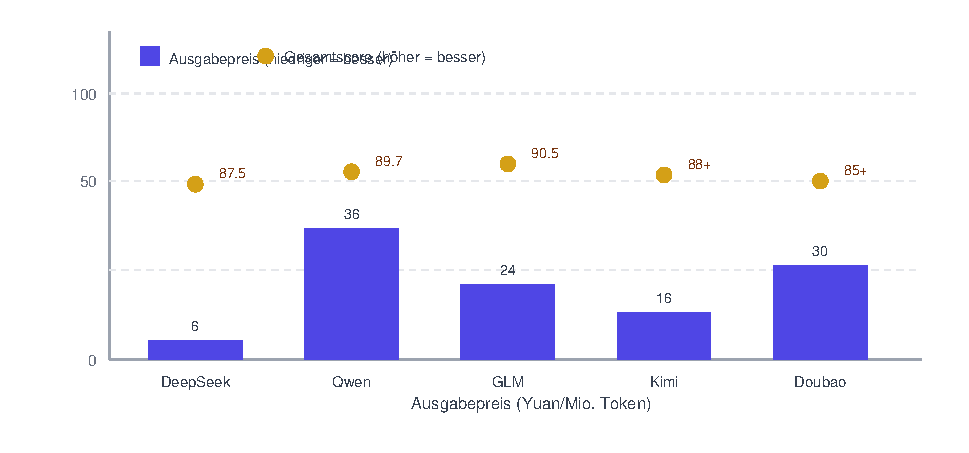
\includegraphics[width=0.92\linewidth]{figures/fig-di-si-shi-er-zhang-1}
\\[2pt]\small Abbildung 4: Preis- und Leistungsvergleich der fünf Modelle (niedrigerer Preis ist besser, höhere Punktzahl ist besser)
\end{center}

\booksection{Der Entscheidungsrahmen für die Modellwahl}

Nachdem du die Modelle kennst: Wie wählst du das richtige für dein Projekt? Hier bekommst du die „Vier-Fragen-Methode“ – beantwortest sie, hast du das passende Modell festgenagelt.

Läuft dein Projekt in China oder international?

In China heimische Modelle wählen

|

International ausländische Modelle möglich

Ist die Kernaufgabe Programmieren oder etwas anderes?

Programmieren Claude oder DeepSeek

|

Anderes weiter prüfen

Brauchst du sehr langen Kontext (>500 000 Token)?

Ja Gemini oder Kimi

|

Nicht nötig weiter prüfen

Budget knapp?

Knapp DeepSeek oder Qwen-turbo

|

Weniger kritisch GPT-5.6 oder Claude

\begin{center}\small\color{gray}Abbildung 5: Die Vier-Fragen-Entscheidungsmethode für die Modellwahl\end{center}

\begin{tcbinfo}{Tipp: Kombinationsstrategie}
Diese Methode ist kein Dogma – viele Szenarien brauchen eine Kombination mehrerer Modelle. Eine gängige Strategie: DeepSeek oder Qwen für die Alltagsentwicklung (günstig, gutes Chinesisch), Claude für kritische Architekturentscheidungen (starke Inferenz, wenig Halluzination), Gemini für Multimodal-Analysen (Bild- und Videobearbeitung). Wechsle das Modell nach Bedarf, statt stur bei einem Modell zu bleiben.

\end{tcbinfo}

\booksection{Erste Schritte mit der API: große Modelle von null anbinden}

Viele KI-Coding-Tutorials zeigen nur die Chat-Oberfläche. Aber echtes „KI-Programmieren“ – deine App ruft ein großes Modell auf – läuft über eine API. Eine API (Application Programming Interface, Programmierschnittstelle) ist ein Kommunikationsprotokoll zwischen Programmen. Über die API kann dein Code die Fähigkeiten eines großen Modells aufrufen, als riefe er eine Funktion auf.

\booksubsection{Was ist ein Token}

Bevor du die API verstehst, musst du den Begriff „Token“ begreifen. Token ist die Grundeinheit, nach der große Modelle abrechnen – denk an sie als „Lese- und Schreibeinheit der KI“. Ein Token entspricht etwa: im Englischen 0,75 Wörtern (4 Zeichen), im Chinesischen 0,5–1 Schriftzeichen. Ein chinesischer Text von 1000 Zeichen verbraucht etwa 1500–2000 Token.

Token sind weder Wortzahl noch Zeichenanzahl. Große Modelle zerlegen Text mit einem eigenen Tokenizer in Token. Dasselbe Wort kann je nach Modell unterschiedlich viele Token belegen – „Künstliche Intelligenz“ kostet in GPT vielleicht 3 Token, in DeepSeek vielleicht 2. Die APIs der meisten Modelle liefern die tatsächlich verbrauchte Tokenzahl zurück; du findest sie in der API-Antwort.

\begin{tcbinfo}{Token-Kosten schnell überschlagen}
1 Mio. chinesische Schriftzeichen entsprechen etwa 1,5 Mio. Token. Verarbeitest du 1 Mio. Zeichen Eingabe plus 1 Mio. Zeichen Ausgabe mit DeepSeek V4 Flash, kostet das rund 0,42 US\$ (ca. 3 RMB); mit Claude Fable 5 für dieselbe Menge rund 60 US\$ (ca. 434 RMB). Genau deshalb wirkt sich die Modellwahl direkt auf deine Projektkosten aus.

\end{tcbinfo}

\booksubsection{Den API-Key besorgen}

Der erste Schritt zur Nutzung der APIs großer Modelle ist der API-Key – eine Zeichenfolge zur Identitätsprüfung. Jeder Modellanbieter hat seine eigene API-Plattform; du registrierst ein Konto und legst einen API-Key an. Hier die Zugänge der API-Plattformen der wichtigsten Modelle samt Ablauf:

\begin{center}
\begin{tabularx}{\linewidth}{|X|X|X|X|}
\hline
\textbf{Modell} & \textbf{API-Plattform} & \textbf{Ablauf} & \textbf{Gratis-Kontingent} \tabularnewline
\hline
DeepSeek & platform.deepseek.com & Registrieren Identität verifizieren API-Key erstellen & Startguthaben für neue Nutzer \tabularnewline
Tongyi Qianwen & bailian.aliyun.com (Bailian-Plattform) & Mit Alibaba-Cloud-Konto anmelden Dienst aktivieren Key erstellen & Gratis-Testphase für neue Nutzer \tabularnewline
Zhipu GLM & open.bigmodel.cn & Registrieren Identität verifizieren API-Key erstellen & Startguthaben für neue Nutzer \tabularnewline
Kimi & platform.moonshot.cn & Registrieren Identität verifizieren API-Key erstellen & begrenztes Gratis-Kontingent \tabularnewline
Doubao & volcengine.com (Volcengine) & Registrieren Ark aktivieren API-Key erstellen & viele Gratis-Token bei der Registrierung \tabularnewline
OpenAI GPT & platform.openai.com & Registrieren Kreditkarte hinterlegen API-Key erstellen & kein Gratis-Kontingent (kostenpflichtig) \tabularnewline
Anthropic Claude & console.anthropic.com & Registrieren Karte hinterlegen API-Key erstellen & kleines Startguthaben für neue Nutzer \tabularnewline
\hline
\end{tabularx}
\end{center}

\begin{center}\small\color{gray}API-Plattformen der wichtigsten Modelle und Key-Bezug (August 2026)\end{center}

\textbf{Sicherheitshinweis: Der API-Key ist wie dein Wallet-Passwort}\par

Ein API-Key ist so wertvoll wie dein Wallet-Passwort – wer ihn hat, kann mit deinem Kontingent Modelle aufrufen. Deshalb: Schreibe den API-Key niemals in den Code (verwende Umgebungsvariablen); lade Code mit Key niemals in ein öffentliches Git-Repository; teile niemals Screenshots, auf denen der Key zu sehen ist. Wenn der Key abhandenkommt, lösch ihn sofort auf der Plattform und leg einen neuen an.

\booksubsection{Der erste API-Aufruf}

Mit deinem API-Key kannst du die API großer Modelle in jeder Programmiersprache aufrufen. Hier das einfachste Beispiel in Python – eine Nachricht an DeepSeek senden und die Antwort holen.

\begin{lstlisting}[language=Python]
# SDK installieren: pip install openai
# DeepSeek ist kompatibel mit dem OpenAI-SDK, direkt nutzbar
from openai import OpenAI
import os

# 1. Client erstellen (API-Key aus der Umgebungsvariable)
client = OpenAI(
    api_key=os.environ.get("DEEPSEEK_API_KEY"),
    base_url="https://api.deepseek.com"
)

# 2. Anfrage senden
response = client.chat.completions.create(
    model="deepseek-chat",  # Modell angeben
    messages=[
        {"role": "system", "content": "Du bist ein Python-Programmierassistent."},
        {"role": "user", "content": "Schreibe eine Quicksort-Funktion."}
    ]
)

# 3. Antwort abholen
print(response.choices[0].message.content)

# 4. Token-Verbrauch ansehen
print(f"Eingabe-Token: {response.usage.prompt_tokens}")
print(f"Ausgabe-Token: {response.usage.completion_tokens}")
print(f"Token gesamt: {response.usage.total_tokens}")
\end{lstlisting}

Die Kernlogik dieses Codes: Client anlegen (mit API-Key und Modelladresse) Nachrichtenliste bauen (system setzt die Rolle, user ist die Nutzereingabe) Anfrage senden Antwort holen. Dieses Muster passt auf praktisch alle Modelle im OpenAI-Format – um das Modell zu wechseln, tauschst du nur api\_key und base\_url. Genau deshalb orientieren sich viele chinesische Modelle am OpenAI-SDK-Format: Entwickler ändern zwei Zeilen Code, und das Modell wechselt – der Migrationsaufwand ist minimal.

Hier die Code-Unterschiede beim Wechsel auf andere Modelle – beachte, dass nur zwei Zeilen geändert werden:

\begin{lstlisting}[language=Python]
# DeepSeek
client = OpenAI(
    api_key=os.environ.get("DEEPSEEK_API_KEY"),
    base_url="https://api.deepseek.com"
)
# model="deepseek-chat"

# Qwen (Bailian-Plattform)
client = OpenAI(
    api_key=os.environ.get("DASHSCOPE_API_KEY"),
    base_url="https://dashscope.aliyuncs.com/compatible-mode/v1"
)
# model="qwen-plus"

# Zhipu GLM
client = OpenAI(
    api_key=os.environ.get("GLM_API_KEY"),
    base_url="https://open.bigmodel.cn/api/paas/v4"
)
# model="glm-4"

# OpenAI GPT
client = OpenAI(
    api_key=os.environ.get("OPENAI_API_KEY"),
    # Standard-base_url reicht
)
# model="gpt-5.6-terra"
\end{lstlisting}

\booksubsection{Streaming-Antworten verarbeiten}

In echten Anwendungen willst du meist nicht warten, bis die KI alles fertig geschrieben hat, um es auf einen Schlag zu zeigen – das lässt Nutzer zu lange warten. Gestreamte Antworten (Streaming) zeigen den Text Zeichen für Zeichen, während die KI ihn erzeugt, und heben das Nutzererlebnis deutlich. Wie bei einer Schreibmaschine, die Buchstabe für Buchstabe ausspuckt – für Nutzer fühlt sich das völlig anders an.

\begin{lstlisting}[language=Python]
# Streaming: Ausgabe Stück für Stück
stream = client.chat.completions.create(
    model="deepseek-chat",
    messages=[
        {"role": "user", "content": "Schreibe ein Tutorial zu Bubblesort in Python"}
    ],
    stream=True  # Streaming einschalten
)

# blockweise empfangen und ausgeben
for chunk in stream:
    if chunk.choices[0].delta.content is not None:
        print(chunk.choices[0].delta.content, end="", flush=True)
# die Ausgabe erscheint Buchstabe für Buchstabe wie bei einer Schreibmaschine
\end{lstlisting}

\booksection{Kaufberatung für Token-Pläne}

Die meisten Modellanbieter rechnen auf zwei Arten ab: nutzungsbasiert (Pay-as-you-go) und als Abo (Token-Plan/Subscription). Den Unterschied zu verstehen hilft dir, die Kosten deutlich zu senken.

\booksubsection{Pay-as-you-go vs. Abo}

\begin{center}
\begin{tabularx}{\linewidth}{|X|X|X|}
\hline
\textbf{Kriterium} & \textbf{Nutzungsbasiert (Pay-as-you-go)} & \textbf{Abo (Subscription)} \tabularnewline
\hline
Abrechnung & zahlen pro verbrauchtem Token & feste Vorauszahlung gegen Kontingent \tabularnewline
Geeignet für & schwankende Nutzung, gelegentliche Aufrufe & gleichmäßige Nutzung, häufige Aufrufe \tabularnewline
Preisvorteil & Standardpreis & 20–50 \% unter Nutzungsbasis \tabularnewline
Flexibilität & jederzeit nutzbar, ohne Bindung & Vorauszahlung nötig; Kontingent kann verfallen \tabularnewline
Überziehen & automatisch nutzungsbasiert & nach Aufbrauchen des Kontingents nutzungsbasiert \tabularnewline
Beispiel-Plattformen & die offiziellen API-Plattformen der Modelle & OpenAI Plus/Pro, Claude Pro, Cursor Pro \tabularnewline
\hline
\end{tabularx}
\end{center}

\begin{center}\small\color{gray}Vergleich der beiden Abrechnungsarten\end{center}

Für Einsteiger empfiehlt sich der Start mit nutzungsbasierter Abrechnung – keine Vorauszahlung, du zahlst nur, was du nutzt. Wenn sich deine Monatsnutzung auf einem Level einpendelt (etwa über 50 RMB pro Monat), denk über den Wechsel zum Abo nach, um den Stückpreis zu senken.

\booksubsection{Die wichtigsten Abo-Pakete im Überblick}

\begin{center}
\begin{tabularx}{\linewidth}{|X|X|X|X|}
\hline
\textbf{Paket} & \textbf{Monatspreis} & \textbf{Enthalten} & \textbf{Geeignet für} \tabularnewline
\hline
ChatGPT Free & gratis & unbegrenzte Text-Chats mit GPT-5.6 Luna & Erstkontakt ohne Vorkenntnisse \tabularnewline
ChatGPT Plus & 20 US\$/Monat & GPT-5.6 Sol, Bilderzeugung, Datenanalyse, Plugin-Zugang & Gelegenheitsnutzer \tabularnewline
ChatGPT Pro & 200 US\$/Monat & alle Modelle unbegrenzt, bevorzugter Zugang zu neuen Funktionen & Intensiv-Profis \tabularnewline
Claude Free & gratis & begrenzte Zahl von Claude-Chats & Erstkontakt ohne Vorkenntnisse \tabularnewline
Claude Pro & 20 US\$/Monat & Claude unbegrenzt, bevorzugter Zugang zu neuen Modellen & Entwickler \tabularnewline
Cursor Free & gratis & begrenzte KI-Vervollständigungen und Chats & für Anfänger zum Ausprobieren \tabularnewline
Cursor Pro & 20 US\$/Monat & unbegrenzte KI-Vervollständigungen, 500 Premium-Anfragen/Monat & Alltagsentwickler \tabularnewline
Cursor Business & 40 US\$/Monat pro Person & Teamzusammenarbeit, Admin-Bereich, Datenschutzmodus & für Teams \tabularnewline
\hline
\end{tabularx}
\end{center}

\begin{center}\small\color{gray}Abo-Pakete der wichtigsten KI-Tools (August 2026)\end{center}

Bei den chinesischen Modellen sehen die Abo-Angebote etwas anders aus. DeepSeek rechnet vor allem nutzungsbasiert ab und hat kein Monatsabo – du lädst Guthaben auf und zahlst nach tatsächlichem Verbrauch. Tongyi Qianwen bietet auf der Bailian-Plattform vorausbezahlte Ressourcenpakete (ein festes Token-Kontingent zum Rabattpreis). Doubao hat auf Volcengine ähnliche Vorauszahlungsangebote. Für Entwickler in China ist die sparsamste Kombination meist: DeepSeek nutzungsbasiert (Alltagsentwicklung) plus Doubaos Gratis-Kontingent (zum Ausprobieren).

\booksubsection{API-Aggregatoren}

Wenn du mehrere Modelle gleichzeitig nutzen willst, sind API-Aggregatoren eine bequeme Wahl. Eine Aggregatorplattform stellt dir einen einzigen API-Key bereit, mit dem du Dutzende Modelle aus aller Welt aufrufen kannst, ohne dich auf jeder Plattform separat zu registrieren.

\begin{center}
\begin{tabularx}{\linewidth}{|X|X|X|X|}
\hline
\textbf{Plattform} & \textbf{Merkmale} & \textbf{Preisvorteile} & \textbf{Geeignete Szenarien} \tabularnewline
\hline
OpenRouter (openrouter.ai) & Aggregator außerhalb Chinas: mit einem Key Modelle aus aller Welt aufrufen & Transparente Preise, Echtzeit-Preisvergleich möglich & Wenn du flexibel zwischen mehreren Übersee-Modellen wechseln willst \tabularnewline
SiliconFlow (siliconflow.cn) & Aggregator in China mit APIs für viele chinesische Modelle & 20–30 \% unter dem offiziellen Preis & Entwickler in China, die mehrere Modelle vergleichen wollen \tabularnewline
Azure OpenAI (Microsoft-Proxy) & Die über Microsoft Azure vermittelte OpenAI-API & Batch API mit 50 \% Rabatt & OpenAI auf Unternehmensniveau, große asynchrone Auftragsmengen \tabularnewline
Baidu Qianfan (qianfan.baidubce.com) & Baidus KI-Cloud-Plattform, mit Modellen wie Ernie (Wenxin) & Gratis-Guthaben für neue Nutzer & Nutzer im Baidu-Ökosystem \tabularnewline
\hline
\end{tabularx}
\end{center}

\begin{center}\small\color{gray}Die wichtigsten API-Aggregatoren (Stand: August 2026)\end{center}

\textbf{Vorsicht vor Fallen: Kaufe keine „Shared Keys“}\par

Kaufe keine sogenannten „Shared API Keys“ auf Plattformen wie Taobao oder Xianyu – diese Keys haben meist eine unklare Herkunft, können jederzeit gesperrt werden und bergen das Risiko von Datenlecks. Beziehe API-Keys immer über offizielle Plattformen oder seriöse Aggregatoren.

\booksubsection{Strategien zur Kostenoptimierung}

Das richtige Modell zu wählen ist nur der erste Schritt; sparsam damit umzugehen ist genauso wichtig. Hier einige praxiserprobte Strategien zur Kostenoptimierung:

\begin{enumerate}
  \item Nutze Cache-Treffer clever. Viele Modelle bieten eine „Cache“-Funktion – enthält deine Anfrage Inhalte, die schon zuvor verarbeitet wurden (z. B. den Systemprompt), wird dieser Teil nur zu einem extrem niedrigen Preis berechnet. Bei DeepSeek kostet ein Cache-Treffer nur 1/60 des normalen Preises. Feste Systemprompts an den Anfang der Nachrichtenliste zu stellen maximiert die Cache-Trefferquote.
  \item Gestaffeltes Routing – einfache Aufgaben mit günstigen Modellen erledigen, komplexe mit teuren. Zum Beispiel DeepSeek V4 Flash für die Textklassifikation (Ausgabe: 2 Yuan pro Million Token) und Claude für den Architekturentwurf (Ausgabe: 181 Yuan pro Million Token). In einem Projekt können 80 \% der Aufrufe mit dem günstigen Modell laufen.
  \item Begrenze die Ausgabelänge. Die API wird nach Ausgabe-Token abgerechnet – je länger die Ausgabe, desto teurer. In Szenarien, die keine langen Ausführungen brauchen, setze den Parameter max\_tokens, um die Ausgabe zu begrenzen und zu verhindern, dass die KI „zu viel um den heißen Brei redet“.
  \item Nutze die Batch API für Aufgaben ohne Echtzeitbedarf. Wenn du viele Aufgaben hast, die keine sofortige Antwort brauchen (etwa Massen-Annotation von Daten oder Dokumentzusammenfassungen), bekommst du mit der Batch API 50 \% Rabatt. OpenAI und Azure bieten diese Funktion beide an.
  \item Überwache den Token-Verbrauch. Die meisten API-Plattformen bieten ein Nutzungs-Dashboard. Schau regelmäßig nach, wie sich der Verbrauch verteilt, finde die Aufrufe mit dem höchsten Token-Verbrauch und optimiere gezielt dort. Eine kleine Anpassung am Prompt (etwa statt „Erkläre bitte ausführlich“ jetzt „Erkläre es bitte in 3 Sätzen“) kann 50 \% der Token sparen.
\end{enumerate}

\begin{center}
\begin{tabularx}{\linewidth}{|X|X|X|X|}
\hline
\textbf{Optimierungsstrategie} & \textbf{Ersparnis} & \textbf{Umsetzungsaufwand} & \textbf{Erläuterung} \tabularnewline
\hline
Cache-Treffer & bis zu 98 \% & Niedrig & Feste Inhalte an den Anfang der Nachrichten stellen \tabularnewline
Gestaffeltes Routing & 50\%-80\% & Mittel & Einfache Aufgaben mit dem günstigen Modell \tabularnewline
Ausgabelänge begrenzen & 30\%-60\% & Niedrig & Den Parameter max\_tokens setzen \tabularnewline
Batch API & 50\% & Niedrig & Batch-Verarbeitung für Aufgaben ohne Echtzeitbedarf \tabularnewline
Prompt-Optimierung & 20\%-50\% & Mittel & Prompts straffen, Redundanz reduzieren \tabularnewline
\hline
\end{tabularx}
\end{center}

\begin{center}\small\color{gray}Strategien zur Kostenoptimierung und ihre Wirkung (Stand: August 2026)\end{center}

\booksection{Praxis: Eine LLM-API in dein Projekt einbinden}

Beenden wir dieses Kapitel mit einer kompletten Praxisübung – einem „KI-Zusammenfassungs-Generator“: Der Nutzer gibt einen langen Text ein, und über eine LLM-API wird eine Zusammenfassung erzeugt. Diese Übung zeigt den kompletten Ablauf eines API-Aufrufs: Umgebungskonfiguration, API-Aufruf, Fehlerbehandlung, Kostenkontrolle.

\begin{lstlisting}[language=Python]
# ai_summarizer.py - KI-Zusammenfassungsgenerator
import os
from openai import OpenAI

# 1. Konfiguration (API-Key aus der Umgebungsvariable, nie hart kodiert)
client = OpenAI(
    api_key=os.environ.get("DEEPSEEK_API_KEY"),
    base_url="https://api.deepseek.com"
)

def summarize(text: str, max_length: int = 200) -> dict:
    """Erzeugt eine Textzusammenfassung

    Args:
        text: zu zusammenfassender Originaltext
        max_length: maximale Länge der Zusammenfassung (Token)

    Returns:
        dict: enthält Zusammenfassung und Token-Verbrauch
    """
    try:
        response = client.chat.completions.create(
            model="deepseek-chat",
            messages=[
                {
                    "role": "system",
                    "content": "Du bist ein Zusammenfassungsgenerator."
                               "Fasse den Text des Nutzers klar und knapp zusammen."
                               "Die Zusammenfassung hat höchstens 3 Sätze."
                },
                {
                    "role": "user",
                    "content": f"Fasse den folgenden Text zusammen:\n\n{text}"
                }
            ],
            max_tokens=max_length,  # begrenzt die Ausgabelänge
            temperature=0.3  # niedrige Temperatur = stabiler
        )

        return {
            "success": True,
            "summary": response.choices[0].message.content,
            "input_tokens": response.usage.prompt_tokens,
            "output_tokens": response.usage.completion_tokens,
            "total_tokens": response.usage.total_tokens
        }

    except Exception as e:
        return {
            "success": False,
            "error": str(e)
        }

# 2. Anwendungsbeispiel
if __name__ == "__main__":
    long_text = """
    (langen Text hier einfügen ...)
    """

    result = summarize(long_text)

    if result["success"]:
        print(f"Zusammenfassung: {result['summary']}")
        print(f"Verbrauchte Token: {result['total_tokens']}")
        # Kostenschätzung: DeepSeek V4 Flash
        cost = result['total_tokens'] * 0.000004  # $\approx$ 0,4 Cent je 1000 Token
        print(f"Geschätzte Kosten: {cost:.4f} Yuan")
    else:
        print(f"Fehler: {result['error']}")
\end{lstlisting}

Dieser Code verkörpert mehrere Best Practices für API-Aufrufe: Der API-Key wird über Umgebungsvariablen gelesen und niemals in den Code geschrieben; die Funktion hat klare Dokumentation und Typhinweise; mit max\_tokens ist die Ausgabelänge begrenzt; temperature steht auf einem niedrigen Wert (0,3) für stabilere Ausgaben; es gibt eine vollständige Fehlerbehandlung; und der Token-Verbrauch wird fürs Kosten-Tracking zurückgegeben. Wenn du die KI diesen Code schreiben lässt, kannst du ihr genau diese Anforderungen nennen – sie ist durchaus in der Lage, das umzusetzen.

Die Schlussbotschaft dieses Kapitels: Modelle sind die "Munition", die Methodik die "Taktik". Die richtige Munition erleichtert den Kampf, aber ohne gute Taktik gewinnt auch die beste Munition keinen Krieg. Du kennst jetzt die Stärken der Modelle und den API-Umgang – dein "Munitionsdepot" ist voll; wie du die Schlacht führst, entscheidet die Denkmethodik aus den vorigen Kapiteln.

\begin{tcbpractice}{Los geht's: Bringe deinen ersten API-Aufruf zum Laufen}
Registriere dich auf einer Plattform für chinesische Modelle (empfohlen: DeepSeek oder Zhipu, beide schenken Neukunden ein Startguthaben), erstelle einen API-Key, trage ihn in die System-Umgebungsvariablen ein (nicht in den Code!) und führe dann den obigen Code für den „ersten API-Aufruf“ aus. In dem Moment, in dem die Antwort der KI ausgegeben wird, hast du die Grenze zwischen „KI nutzen“ und „KI-Anwendungen bauen“ überschritten.

\end{tcbpractice}

\begin{tcbsummary}{Kapitelfazit}
\begin{itemize}
  \item Internationale Top 3: GPT-5.6 (der ausgewogene Allrounder), Claude (König des Programmierens + nur 1 \% Halluzinationsrate), Gemini (Multimodal-König + 2 Mio. Kontext)
  \item Chinesische Top 5: DeepSeek V4 (Preis-Leistungs-König, Preiserhöhungs-Ankündigungen beachten), Qwen3.7 (Unternehmensklasse), GLM-5.1 (Nr. 1 in China bei SWE), Kimi K3 (extrem lange Texte), Doubao (kostenloser Einstieg)
  \item Die Vier-Fragen-Methode: Wo läuft das Modell? Programmieren oder etwas anderes? Sehr langer Kontext? Budgetkritisch?
  \item Token sind die Abrechnungseinheit: 1 chinesisches Zeichen $\approx$ 1,5–2 Token; 1 Million Zeichen $\approx$ 1,5 Millionen Token
  \item API-Key = Wallet-Passwort: in Umgebungsvariablen verwalten, niemals hardcoden, nie zu Git hochladen
  \item Chinesische Modelle sind meist kompatibel zum OpenAI-SDK: Für einen Modellwechsel genügen zwei geänderte Zeilen, api\_key und base\_url
  \item Fünf Spartipps: Cache-Treffer nutzen, gestaffeltes Routing, Ausgabe begrenzen, Batch API, Verbrauch überwachen
\end{itemize}

\end{tcbsummary}

\bookchapter{Kapitel 43: Dialog-Engineering – Dialogtechniken für effiziente Zusammenarbeit mit der KI}

\chapterintro{Dialog ist die zentrale Interaktionsform beim KI-Programmieren. Aber Achtung: „Dialog“ ist nicht gleich „Plaudern“ – ein effizientes KI-Programmiergespräch ist eine strukturierte Kommunikationstechnik, die wir „Dialog-Engineering“ nennen. Es untersucht: Wie bekommt man mit möglichst wenigen Dialogrunden die höchste Codequalität? Ganz platt gesagt: Dieses Kapitel zeigt dir, wie du mit der KI „klar redest“.}

\booksection{Ebenen-Strategie für Prompts}

Der Dialog mit der KI lässt sich in drei Ebenen gliedern, und jede Ebene übernimmt eine eigene Aufgabe. Wenn du diese drei Ebenen verstehst, kannst du effiziente Prompts wie mit Bauklötzen zusammenbauen.

\begin{center}
\begin{tabularx}{\linewidth}{|X|X|X|X|}
\hline
\textbf{Ebene} & \textbf{Funktion} & \textbf{Beispiel} & \textbf{Häufigkeit} \tabularnewline
\hline
Systemebene & Legt die Rolle der KI und die globalen Rahmenbedingungen fest & „Du bist ein React-Experte, der Code muss in TypeScript geschrieben werden“ & Einmal zu Beginn des Projekts festlegen \tabularnewline
Aufgabenebene & Beschreibt die konkrete anstehende Aufgabe & „Baue eine Formularkomponente mit Feldern für Benutzername und Passwort“ & Zu Beginn jeder Aufgabe geben \tabularnewline
Feedback-Ebene & Bewertet und korrigiert die Ergebnisse der KI & „Beim Passwortfeld fehlt der Umschalter für Anzeigen/Verbergen, bitte ergänzen“ & Je nach Qualität der Ergebnisse geben \tabularnewline
\hline
\end{tabularx}
\end{center}

\begin{center}\small\color{gray}Die drei Ebenen des Dialog-Prompts\end{center}

Prompts der Systemebene stehen meist in der Projektgedächtnis-Datei (z. B. CLAUDE.md) und müssen nicht bei jedem Dialog wiederholt werden. Die Aufgabenebene nutzt du im Dialog am häufigsten – sie sollte die drei Elemente „Was ist zu tun“, „Mit welcher Technik“, „Welche Rahmenbedingungen“ enthalten. Die Feedback-Ebene verlangt das meiste Können – gutes Feedback lässt die KI präzise korrigieren, schlechtes Feedback lässt sie nur erneut raten.

\begin{tcbinfo}{Tipp: Feedback in drei Schritten}
Eine praktische Feedback-Vorlage lautet: „Problem benennen + Erwartung erklären + Kontext liefern“. Zum Beispiel: „Die Fehlerbehandlung in Zeile 25 nutzt nur console.log (Problem benennen), in der Produktionsumgebung sollte ein einheitlicher Fehlerbehandler mit nutzerfreundlichen Meldungen zum Einsatz kommen (Erwartung erklären), im Projekt gibt es dafür eine handleError-Funktion (Kontext liefern)“. Ein solches Feedback ist zehnmal wirksamer als „Ändere mal die Fehlerbehandlung“.

\end{tcbinfo}

\booksection{Debug-Dialoge: Fehler so beschreiben, dass die KI sie schnell findet}

Debugging ist eine der häufigsten Situationen beim KI-Programmieren. Wenn du auf einen Bug stößt, entscheidet die Beschreibung des Problems gegenüber der KI direkt darüber, wie schnell sie es eingrenzen und beheben kann. Hier die vier Kernpunkte für Debug-Dialoge:

\begin{enumerate}
  \item Lass die KI die Originaldaten „sehen“, nicht nur deine Wiedergabe. Hänge Fehlerprotokolle, Stacktraces und den relevanten Code direkt per @-Verweis an, statt sie mit „da gab's wohl irgendeinen Fehler“ zu umschreiben. Mit den Originaldaten arbeitet die KI genauer als mit deiner Interpretation.
  \item Beschreibe den Unterschied zwischen erwartetem und tatsächlichem Verhalten. „Ich erwarte, dass der Klick auf den Button zur Startseite führt (erwartet), aber tatsächlich passiert beim Klick nichts (tatsächlich)“ – diese Beschreibung nützt viel mehr als „Der Button ist kaputt“.
  \item Liefere Reproduktionsschritte. „Erst den Benutzernamen eingeben, dann auf den Anmelde-Button klicken – und der Fehler erscheint“ – Reproduktionsschritte lassen die KI deinen Weg nachspielen und das Problem leichter eingrenzen.
  \item Sage klar, was du schon probiert hast. „Ich habe die Netzwerkanfrage geprüft, sie antwortet mit 200, die Daten sind in Ordnung“ – so kann die KI bereits Geprüftes ausschließen und keine Zeit mit doppelter Suche verschwenden.
\end{enumerate}

Schlechte Fehlerbeschreibung

\begin{lstlisting}
Auf den Buttonklick reagiert nichts, schau mal nach
\end{lstlisting}

Gute Fehlerbeschreibung

\begin{lstlisting}
Nach dem Klick auf den Anmelde-Button reagiert die Seite nicht. Erwartetes Verhalten: Nach dem Klick wird zur Seite /home navigiert Tatsächliches Verhalten: Nach dem Klick passiert nichts, die Konsole zeigt keinen Fehler Reproduktionsschritte: 1. Auf der Login-Seite Benutzername admin und Passwort 123456 eingeben 2. Auf den Button „Anmelden“ klicken 3. Die Seite reagiert nicht Bereits geprüft: - Netzwerkanfrage normal, Rückgabe 200 - onClick-Ereignis ist gebunden - Code der Komponente LoginButton geprüft Relevante Dateien: @src/components/LoginButton.tsx @src/pages/Login.tsx
\end{lstlisting}

\booksection{Iterationsstrategie: Kleine schnelle Schritte vs. großes Refactoring}

Beim KI-Programmieren gibt es zwei grundlegende Iterationsstrategien für unterschiedliche Situationen. Wer den Unterschied versteht, trifft in jeder Lage die richtige Wahl.

Die Strategie der „kleinen schnellen Schritte“ eignet sich für Funktionsentwicklung und Bugfixes. Ihr Kern: Die KI macht jeweils nur eine kleine Änderung, und erst nach bestandener Prüfung kommt die nächste. Vorteil: Jeder Schritt ist prüfbar und rückholbar, das Risiko bleibt kontrollierbar. Nachteil: Es geht langsamer und braucht viele Dialogrunden. Geeignet für: Entwicklung neuer Funktionen, exploratives Vorgehen, wenn die beste Lösung noch unklar ist, und vorsichtiges Iterieren, solange du den Ergebnissen der KI noch nicht ganz traust.

Die Strategie des „großen Refactorings“ eignet sich für großflächige Änderungen mit klarem Ziel. Ihr Kern: Das vollständige Ziel wird auf einmal beschrieben, und die KI plant und führt die gesamte Änderung selbstständig aus. Vorteil: Es geht schnell, und weil die KI das Gesamtbild sieht, trifft sie bessere Architekturentscheidungen. Nachteil: Das Risiko ist hoch – versteht die KI etwas falsch, ist die Korrektur aufwendig. Geeignet für: klar umrissene Architektur-Upgrades, groß angelegte Code-Migrationen und Refactorings mit ausreichender Testabdeckung.

\begin{center}
\begin{tabularx}{\linewidth}{|X|X|X|}
\hline
\textbf{Aspekt} & \textbf{Kleine schnelle Schritte} & \textbf{Großes Refactoring} \tabularnewline
\hline
Umfang pro Änderung & Ein Funktionspunkt oder ein Bug & Ein Modul oder eine Architekturebene \tabularnewline
Prüffrequenz & Direkt nach jeder Änderung prüfen & Prüfen, sobald alle Änderungen fertig sind \tabularnewline
Dialogrunden & Viele (5–10 Runden pro Funktion) & Wenige (1–3 Runden pro Modul) \tabularnewline
Risiko & Niedrig, jeder Schritt ist rückholbar & Hoch, Korrekturen bei Abweichungen sind aufwendig \tabularnewline
Geeignete Szenarien & Neue Funktionen, explorative Entwicklung & Refactoring und Migration mit klarem Ziel \tabularnewline
Voraussetzungen & Keine besonderen Anforderungen & Testabdeckung erforderlich \tabularnewline
\hline
\end{tabularx}
\end{center}

\begin{center}\small\color{gray}Vergleich der beiden Iterationsstrategien\end{center}

In der Praxis kombiniert man beide Strategien oft. Bei einem Modul-Refactoring lässt du die KI zunächst mit dem „großen Refactoring“ einen Gesamtplan erstellen; nach der Prüfung des Plans setzt du ihn mit „kleinen schnellen Schritten“ Stück für Stück um. So behältst du die Gesamtübersicht und kontrollierst zugleich das Ausführungsrisiko.

\booksection{Kontextmanagement bei langen Dialogen}

Mit jeder zusätzlichen Dialogrunde musst du den Kontext aktiv verwalten, damit die KI frühere Informationen nicht „vergisst“. Hier einige praktische Techniken fürs Kontextmanagement.

Erstens: Kerninformationen „verankern“. Schreibe die wichtigsten Rahmenbedingungen zu Beginn des Dialogs klar nieder und wiederhole sie im weiteren Verlauf passend. Zum Beispiel: „Denk dran, unsere Daten liegen im localStorage, eine Datenbank können wir nicht benutzen“ – wiederhole diese Bedingung bei passenden Änderungswünschen, damit die KI sie nicht vergisst.

Zweitens: Nutze die Technik „Zusammenfassen und Weitermachen“. Wenn der Dialog sehr lang geworden ist, lass die KI „den bisherigen Stand und die offenen Aufgaben zusammenfassen“, und starte dann einen neuen Dialog mit dieser Zusammenfassung als Ausgangspunkt. So bleibt der wichtige Kontext erhalten, ohne dass der lange Dialog sich abnutzt.

Drittens: „Ein Dialog, eine Aufgabe“. Das ist die einfachste und zugleich wirksamste Strategie fürs Kontextmanagement. Jeder Dialog behandelt nur eine Aufgabe oder einen Funktionspunkt; danach startest du einen neuen Dialog für die nächste. Das begrenzt die Dialoglänge ganz natürlich und hält den Kontext klar.

Viertens: Nutze die Kontextfunktionen deiner Tools. Die meisten KI-Programmier-Tools haben einen Button „Kontext löschen“ oder „Neue Sitzung“ – wenn du spürst, dass die Antworten der KI nachlassen, zögere nicht: Neue Sitzung. Etwas Dialoghistorie zu verlieren ist viel besser, als sich weiter durch einen abgenutzten Kontext zu kämpfen.

\begin{tcbpractice}{Los geht's: Spiel für deine KI einmal den „Patienten“}
Baue absichtlich eine kleine Seite im Browser und erzeuge einen Bug (etwa einen Button, der nicht reagiert). Beschreibe das Problem dann einmal vollständig nach dem Muster der „guten Fehlerbeschreibung“ aus diesem Kapitel: Originaldaten, erwartet vs. tatsächlich, Reproduktionsschritte, bereits Geprüftes. Spüre, wie unterschiedlich schnell die KI das Problem eingrenzt – dann verstehst du, warum „Probleme beschreiben“ selbst ein Handwerk ist.

\end{tcbpractice}

\begin{tcbsummary}{Kapitelfazit}
\begin{itemize}
  \item Prompt in drei Ebenen: Systemebene (in die Gedächtnis-Datei), Aufgabenebene (Was + Technik + Rahmenbedingungen), Feedback-Ebene (Problem + Erwartung + Kontext)
  \item Debugging in vier Punkten: Originaldaten liefern, erwartet vs. tatsächlich, Reproduktionsschritte, bereits Geprüftes
  \item Kleine schnelle Schritte: wenig Risiko, viele Runden, ideal für neue Funktionen; großes Refactoring: hohes Risiko, wenige Runden, braucht Tests als Absicherung
  \item Kontextmanagement in vier Zügen: Kerninfos verankern, Zusammenfassen und Weitermachen, ein Dialog pro Aufgabe, konsequent neue Sitzung starten
\end{itemize}

\end{tcbsummary}

\bookchapter{Kapitel 44: Praxis von 0 auf 1 – Der komplette Ablauf eines Projekts}

\chapterintro{Die Theorie sitzt – jetzt wird gewerkelt. Dieses Kapitel ist kein einfaches „Tipp-nach“-Tutorial, sondern eine Praxis-Methodik für „Wie denke ich? Wie frage ich? Wie prüfe ich?“. An drei Projekten mit steigendem Schwierigkeitsgrad zeigen wir den kompletten Gedankengang von der Anforderung bis zum fertigen Produkt. Diese Vorgehensweise funktioniert, egal welches Tool du nutzt.}

\booksection{Projekt 1: Eine schlanke persönliche Tool-Seite (Einsteiger)}

\booksubsection{Über die Anforderungen nachdenken}

Ziel: eine persönliche Tool-Seite mit Einstiegen zu 3–4 praktischen Mini-Tools. Ein reines Frontend-Projekt, ohne Backend und Datenbank. Wichtig ist nicht, wie komplex die Tools sind, sondern dass du den kompletten Weg „von der Anforderung zum fertigen Produkt“ durchlebst.

Entlang der fünf Anforderungselemente: Who – für den persönlichen Gebrauch. What – eine Webseite, die Einstiege zu Tools zeigt. Why – die häufig genutzten Tools auf einer Seite sammeln, damit sie schnell erreichbar sind. How – eine einzelne HTML-Datei mit CSS und JS, ohne Framework. Constraint – in 30 Minuten fertig, ohne Deployment.

\booksubsection{Die Anweisung geben}

Nach dem Prinzip „Think Before Coding“ sollte deine Anweisung genug Informationen enthalten, damit die KI das Ziel versteht – aber nicht jedes Umsetzungsdetail vorgeben:

\begin{lstlisting}
Erstelle eine persönliche Tool-Webseite mit diesen Anforderungen:
1. HTML in einer einzigen Datei (inline CSS und JS), ohne Frameworks
2. Dunkles Thema, moderner minimalistischer Stil
3. Zeige 4 Tool-Karten:
   - Textzusammenfasser
   - Wortzähler
   - Farbwähler
   - QR-Code-Generator
4. Jede Karte mit Symbol, Titel und kurzer Beschreibung
5. Die Karten haben eine Hover-Animation
6. Responsives Layout, auf dem Handy benutzbar
7. Oben eine Titelleiste
Gib direkt die vollständige HTML-Datei.
\end{lstlisting}

\booksubsection{Abnahme und Iteration}

Sobald die KI den Code liefert, nimmst du die Abnahme entlang der drei Prüfebenen vor. Erste Ebene, Funktionsprüfung: Lässt sich die Datei im Browser öffnen? Werden alle 4 Karten angezeigt? Funktioniert die Hover-Animation? Zweite Ebene, Grenzfallprüfung: Ist das Layout bei Handybildschirmgröße in Ordnung? Brechen die Karten bei sehr schmalen Fenstern sauber um? Dritte Ebene, Architekturprüfung: Ist der Code lesbar? Steht das CSS inline in einem style-Tag? Gibt es auffällige Redundanzen?

Willst du auch die Funktion eines Tool-Kartens umsetzen (statt nur des Einstiegs), ergänze sie nach und nach – jedes Mal eine Funktion, und erst nach der Prüfung die nächste. Genau das ist die Strategie der „kleinen schnellen Schritte“ in der Praxis.

\booksection{Projekt 2: Full-Stack-Ausgabenverwaltung (Fortgeschrittene)}

\booksubsection{Anforderungsdenken und PRD}

Ziel: eine Full-Stack-App zur Ausgabenverwaltung mit Frontend, Backend und Datenbank. Dieses Projekt ist deutlich komplexer als das erste und nutzt die Anforderungs-Engineering-Methoden aus Kapitel 40.

Schreibe zuerst das PRD. Nach der Vorlage aus Abschnitt 3 von Kapitel 40 formulierst du Projektüberblick, Funktionsliste, technische Lösung, Datenmodell und Entwicklungsplan. Bei der technischen Lösung gilt das Prinzip „Simplicity First“ – im Frontend React, aber ohne komplexe State-Verwaltung wie Redux; im Backend Node.js, aber ohne Microservices; als Datenbank SQLite statt PostgreSQL (in der Entwicklungsphase).

Der Entwicklungsplan zerfällt in 5 Schritte: Schritt 1: Backend-API-Skelett (Express-Server + SQLite + CRUD-Endpunkte); Schritt 2: Grundseiten des Frontends (Eintragsliste + Hinzufügen-Formular); Schritt 3: Frontend und Backend verbinden (API-Aufrufe + Datenanzeige); Schritt 4: Kategorien und Filter; Schritt 5: Monatsbilanz und einfache Diagramme. Nach jedem Schritt liegt etwas „Benutzbares“ vor.

\booksubsection{Die Projektgedächtnis-Datei anlegen}

Lege vor dem ersten Code die Projektgedächtnis-Datei an. Das ist die Kernpraxis des Context-Engineerings – so weiß die KI zu Beginn jedes Dialogs, worum es im Projekt geht.

\begin{lstlisting}
# Projekt: Full-Stack-Ausgaben-App
## Überblick
Ausgaben-App mit Erfassung von Einnahmen und Ausgaben, Kategorien und Monatsübersichten.
## Tech-Stack
- Frontend: React + TypeScript + Vite
- Backend: Node.js + Express + TypeScript
- Datenbank: SQLite (über better-sqlite3)
- Geteilte Typen für Frontend und Backend
## API-Konventionen
- Basispfad: /api
- Antwortformat: { success: boolean, data: any, error: string }
- RESTful-Stil
## Datenmodell
Record { id, amount, type, category, note, date }
## Code-Konventionen
- TypeScript im Strict-Modus
- Einrückung mit 2 Leerzeichen
- Funktionen mit JSDoc-Kommentar
- Kommentare und Commit-Meldungen auf Deutsch
\end{lstlisting}

\booksubsection{Schrittweise umsetzen}

Arbeite den Entwicklungsplan ab und nutze für jeden Schritt einen eigenen Dialog. Hier ein Beispiel für die Anweisung des ersten Schritts:

\begin{lstlisting}
Ich brauche das Grundgerüst der Backend-API.
Anforderungen:
1. Express-Server, Port 3001
2. SQLite-Datenbank, Tabelle records
3. Felder der Tabelle records:
   id (TEXT PRIMARY KEY)
   amount (REAL)
   type (TEXT: 'income'|'expense')
   category (TEXT)
   note (TEXT)
   date (TEXT: YYYY-MM-DD)
4. CRUD-Endpunkte:
   GET /api/records - alle Einträge abrufen
   POST /api/records - Eintrag anlegen
   PUT /api/records/:id - Eintrag aktualisieren
   DELETE /api/records/:id - Eintrag löschen
5. Middleware für Fehlerbehandlung
Gib die vollständige Backend-Code-Struktur.
\end{lstlisting}

Beachte die Eigenschaften dieser Anweisung: Sie beschreibt nur den aktuellen Schritt (das Backend-Skelett) und mischt keine Frontend-Wünsche hinein; sie nennt Felder und Endpunkte ausdrücklich (gibt der KI genügend Rahmen), überlässt die konkrete Umsetzung aber der KI; sie folgt dem Prinzip „Goal-Driven Execution“ – sie sagt, „was“ zu tun ist, nicht „wie“.

Sobald die KI den Code liefert, prüfe sofort: Starte den Server und teste jeden Endpunkt mit curl oder Postman. Wenn alles passt, öffnest du einen neuen Dialog für Schritt 2 (Grundseiten des Frontends). Jeder Schritt folgt dem Kreislauf „Anweisung – Prüfung – neuer Dialog“.

\booksection{Projekt 3: KI-gestützte App (Profi)}

\booksubsection{Projektidee}

Ziel: eine App, die eine LLM-API einbindet – etwa ein „KI-Lernassistent“: Der Nutzer gibt Lernstoff ein, die KI erstellt Zusammenfassungen, verknüpft Wissenspunkte und schlägt Lernressourcen vor. Das Besondere an diesem Projekt: Deine App ruft selbst KI auf, und du musst neue Probleme lösen – API-Aufrufe, Prompt-Engineering, Fehlerbehandlung und mehr.

Die wichtigste Lektion dieses Projekts: Wenn du „mit KI Code schreiben lässt, der KI aufruft“, musst du aufs Prompt-Engineering besonders achten. Auch die Prompts, mit denen deine App die LLM-API aufruft, sollten den Prinzipien dieses Leitfadens folgen – klar, prägnant, zielorientiert.

\booksubsection{Wichtige technische Punkte}

Dieses Projekt bringt ein paar technische Punkte mit, die in den ersten beiden Projekten nicht vorkamen:

\begin{itemize}
  \item Verwaltung der API-Schlüssel: Schlüssel gehören niemals in den Code – verwalte sie über Umgebungsvariablen;
  \item Verarbeitung von Streaming-Antworten: LLMs antworten meist als Stream, der Zeichen für Zeichen angezeigt werden muss;
  \item Kontrolle des Token-Verbrauchs: LLMs werden pro Token abgerechnet, die App muss den Verbrauch steuern;
  \item Verwaltung von Prompt-Vorlagen: verschiedene Funktionen brauchen verschiedene Prompt-Vorlagen – strukturiert gepflegt.
\end{itemize}

All diese Punkte kann die KI für dich umsetzen – aber du musst das „Warum“ hinter jedem Punkt verstehen: Warum dürfen Schlüssel nicht hardcodiert werden? Warum braucht es Streaming-Antworten? Warum muss der Token-Verbrauch kontrolliert werden? Erst wenn du das „Warum“ verstehst, kannst du beurteilen, ob die Lösung der KI stimmig ist.

\booksection{Universelle Praxis-Checkliste}

Groß oder klein – hier ist eine universelle Checkliste für KI-Programmierprojekte. Gehe sie bei jedem neuen Projekt einmal durch, damit kein wichtiger Schritt fehlt.

\begin{center}
\begin{tabularx}{\linewidth}{|X|X|X|}
\hline
\textbf{Phase} & \textbf{Was tun?} & \textbf{Zugehöriges Prinzip} \tabularnewline
\hline
1. Anforderungen durchdenken & Die fünf Anforderungselemente durchgehen und klären, was entstehen soll & Think Before Coding \tabularnewline
2. Anforderungen zerlegen & Große Anforderungen in kleine, einzeln prüfbare Schritte zerlegen & Simplicity First \tabularnewline
3. PRD schreiben & Als strukturiertes Dokument festhalten, als Referenz dienen & Goal-Driven \tabularnewline
4. Gedächtnis-Datei anlegen & CLAUDE.md oder eine vergleichbare Datei anlegen & Harness Engineering \tabularnewline
5. Schrittweise umsetzen & Ein Dialog pro Schritt: Anweisung – Prüfung – nächster Schritt & Surgical Changes \tabularnewline
6. Testen und Prüfen & Direkt nach jedem Schritt die korrekte Funktion testen & Iterate \& Verify \tabularnewline
7. Code-Review & Architektur, Sicherheit und Wartbarkeit prüfen & Iterate \& Verify \tabularnewline
8. Iterieren und Verbessern & Auf Basis von Test- und Reviewergebnissen weiter verbessern & Iterate \& Verify \tabularnewline
\hline
\end{tabularx}
\end{center}

\begin{center}\small\color{gray}Universelle Praxis-Checkliste fürs KI-Programmieren\end{center}

\begin{tcbpractice}{Los geht's: Diese Woche „Projekt 1“ abschließen}
Mach die „persönliche Tool-Seite“ aus Abschnitt 1 von Kapitel 44 zu deiner ersten KI-Programmieraufgabe: Nimm dir 5 Minuten für die fünf Anforderungselemente, schick die Anweisung an die KI (welches Tool auch immer) und nimm die Abnahme mit der dreistufigen Prüfung vor. In 30 Minuten ist sie fertig – und dein erstes KI-Programmierprojekt ist da. Speichere es gut auf: Es ist dein Andenken an den Sprung vom „Leser“ zum „Praktiker“.

\end{tcbpractice}

\begin{tcbsummary}{Kapitelfazit}
\begin{itemize}
  \item Projekt 1 (Einsteiger): reine Frontend-Tool-Seite – den kompletten Ablauf erleben, in 30 Minuten machbar
  \item Projekt 2 (Fortgeschrittene): Full-Stack-Ausgabenverwaltung – PRD + Gedächtnis-Datei + Umsetzung in 5 Schritten, jeder Schritt „benutzbar“
  \item Projekt 3 (Profi): KI-Lernassistent – mit KI Code schreiben, der KI aufruft; aufs Prompt-Engineering achten
  \item Der universelle Ablauf in 8 Schritten: Anforderungen durchdenken zerlegen PRD Gedächtnis-Datei schrittweise umsetzen testen Review iterieren
  \item Jeder Schritt folgt dem Kreislauf „Anweisung – Prüfung – neuer Dialog“
\end{itemize}

\end{tcbsummary}

\bookchapter{Kapitel 45: Qualitätssicherung – KI-Code zuverlässig machen}

\chapterintro{KI-Code hat eine Eigenheit: Er „sieht meist richtig aus“ – sauber benannte Variablen, ausführliche Kommentare, klare Logik. Aber „richtig aussehen“ ist nicht „wirklich richtig“. Versteckte Probleme in KI-Code sind oft schwerer zu finden als in handgeschriebenem Code, denn die hohe Oberflächenqualität macht sorglos. Dieses Kapitel zeigt dir, wie du für KI-Code ein wirksames Qualitätssicherungssystem aufbaust – mit den drei Verteidigungslinien Tests, Review und Versionskontrolle wird aus „sieht richtig aus“ ein „ist wirklich richtig“.}

\booksection{Testgetrieben: Die KI Tests schreiben lassen}

Tests sind die erste Verteidigungslinie der Qualitätssicherung beim KI-Programmieren. Die gute Nachricht: Die KI Tests schreiben zu lassen ist leichter und zuverlässiger, als sie Funktionscode schreiben zu lassen – denn das erwartete Verhalten eines Tests ist eindeutig, und der typische Fall „sieht richtig aus, ist aber falsch“ tritt seltener auf.

Der testgetriebene Ablauf beim KI-Programmieren: Zuerst lässt du die KI den Funktionscode schreiben; sobald die Grundfunktion läuft, lässt du sie sofort Testfälle schreiben. Die Testfälle sollten Normalfälle, Grenzfälle und Ausnahmefälle abdecken. Danach lässt du die KI den Funktionscode anhand des Testfeedbacks korrigieren. Der Vorteil dieses Ablaufs: Sind die Tests einmal geschrieben, sind sie ein dauerhaftes Prüfinstrument – jede spätere Änderung kannst du mit einem Testlauf darauf hin kontrollieren, dass kein Regressionsfehler entsteht.

\begin{lstlisting}
Schreibe Unit-Tests für die Funktion calculate_discount.
Die Testfälle sollen abdecken:
1. Normalfall:
   - 100 Yuan mit 20 % Rabatt -> 80
   - 200 Yuan mit 50 % Rabatt -> 100
2. Grenzfälle:
   - 0 Yuan mit 20 % Rabatt -> 0
   - 100 Yuan ohne Rabatt -> 100 (keine Ermäßigung)
   - 100 Yuan zum Vollpreis -> 100 (voller Preis)
3. Fehlerfälle:
   - negativer Preis -> muss einen Fehler werfen
   - Rabatt > 1 -> muss einen Fehler werfen
   - Eingabe keine Zahl -> Muss einen Fehler werfen
Verwende das Vitest-Framework und gib die vollständige Testdatei.
\end{lstlisting}

Beachte die Eigenschaft dieser Anweisung: Sie listet die drei Testfallarten ausdrücklich auf (Normal-, Grenz- und Ausnahmefälle) und lässt der KI keinen Spielraum für „selektives Testen“. Manchmal schreibt die KI nur Tests für den Normalweg, um schnell fertig zu wirken – wenn du alle Kategorien ausdrücklich auflistest, vermeidest du das.

\booksection{Techniken fürs Code-Review}

Auch mit Testabdeckung musst du den KI-Code selbst durchsehen. Ein Code-Review heißt nicht, alles Zeile für Zeile zu lesen – das kostet zu viel Zeit und hängt zu sehr von deinem Können ab. Ein wirksames Review von KI-Code konzentriert sich auf folgende Kerndimensionen:

\begin{center}
\begin{tabularx}{\linewidth}{|X|X|X|}
\hline
\textbf{Review-Dimension} & \textbf{Worauf achten} & \textbf{Typische Probleme} \tabularnewline
\hline
Sicherheit & Eingabeprüfung, Umgang mit Schlüsseln, Schutz vor SQL-Injection & Die KI vergisst oft die Eingabeprüfung und schreibt Schlüssel direkt in den Code \tabularnewline
Fehlerbehandlung & Werden Ausnahmen abgefangen? Sind die Fehlermeldungen sinnvoll? & Die KI nutzt gern leere catch-Blöcke oder nur console.log \tabularnewline
Leistung & Gibt es offenkundige Leistungsprobleme wie N+1-Abfragen oder Endlosschleifen? & Die KI schreibt manchmal Algorithmen in O(n²) \tabularnewline
Wartbarkeit & Ist die Code-Struktur klar? Sind die Bezeichner aussagekräftig? & Die KI erzeugt gelegentlich überabstrahierten Code \tabularnewline
Abhängigkeitsverwaltung & Sind die eingesetzten Abhängigkeiten nötig? Sind die Versionen klar definiert? & Die KI bindet gern unnötige Bibliotheken ein \tabularnewline
\hline
\end{tabularx}
\end{center}

\begin{center}\small\color{gray}Kerndimensionen des KI-Code-Reviews\end{center}

Beim Review musst du nicht alles selbst durchgehen – lass die KI die erste Runde übernehmen. Anweisung zum Beispiel: „Prüfe bitte Sicherheit, Fehlerbehandlung und Leistung dieses Codes und nenne potenzielle Probleme.“ Die Selbstprüfungsfähigkeit der KI wird immer besser; sie ersetzt das menschliche Review zwar nicht vollständig, filtert aber die meisten offenkundigen Probleme heraus.

\booksection{Versionskontrolle: Die Rolle von Git beim KI-Programmieren}

Git ist beim KI-Programmieren noch wichtiger als in der klassischen Programmierung. Da jede KI-Änderung unvorhersehbare Folgen haben kann, brauchst du ein verlässliches „Rückgängig“ – die Versionskontrolle ist genau dieses Rückgängig.

Die Git-Best-Practice beim KI-Programmieren lautet: „Häufig committen, in kleinen Schritten vorangehen.“ Nach jedem überprüfbaren Funktionspunkt kommt ein Commit. So kannst du, wenn eine Änderung der KI Probleme macht, gezielt zum letzten funktionierenden Stand zurückkehren, statt alle Arbeit über den Haufen zu werfen.

Ein weiterer praktischer Trick ist die „Branch-Isolation“. Für KI-Änderungen mit ungewissem Ausgang (etwa ein großes Refactoring) legst du zuerst einen neuen Branch an und arbeitest dort. Gefällt das Ergebnis, mergest du in den Hauptbranch zurück; gefällt es nicht, löschst du den Branch einfach – der Hauptbranch bleibt unberührt. Das ist viel sicherer, als immer wieder am Hauptbranch herumzubasteln.

\begin{enumerate}
  \item Vor jeder KI-Änderung: Vergewissere dich, dass das Arbeitsverzeichnis sauber ist (keine uncommitteten Änderungen). Dann kannst du bei einem misslungenen Ergebnis mit git checkout . schnell zurücksetzen.
  \item Sobald die KI eine Änderung gemacht hat und die Prüfung bestanden ist, sofort committen. Die Commit-Meldung beschreibt, was die Änderung bewirkt, z. B. „feat: Benutzerregistrierung hinzugefügt“.
  \item Für große Refactorings zuerst einen Branch anlegen: git checkout -b refactor/auth-system. Die Änderungen auf dem Branch fertigstellen und erst nach bestandenen Tests mergen.
  \item Gewöhne dir an, den Diff anzusehen. Nach jeder KI-Änderung zeigt dir git diff, was genau geändert wurde. Das hilft dir nicht nur, Probleme zu entdecken, sondern auch, vom Code zu lernen.
\end{enumerate}

\booksection{Häufige Stolperfallen und wie du sie vermeidest}

Beim KI-Programmieren gibt es einige Stolperfallen, die immer wieder auftauchen und in die fast alle Einsteiger tappen. Wer sie kennt, erspart sich viele Umwege.

\booksubsection{Falle 1: Die Vertrauensfalle}

„Der Code der KI sieht so professionell aus, da kann doch nichts falsch sein?“ – das ist die gefährlichste Falle. KI-generierter Code ist oberflächlich sehr ordentlich – saubere Namen, ausführliche Kommentare, klare Struktur – und genau dieser „professionelle Schein“ macht sorglos. Aber ordentliche Oberfläche heißt nicht korrekte Logik. Gegenmittel: Immer per Tests verifizieren, niemals danach urteilen, ob etwas „richtig aussieht“.

\booksubsection{Falle 2: Die Aufbläh-Falle}

„Da die KI mir Code schreibt, warum nicht gleich ein bisschen mehr ausbauen?“ – das führt zu aufgeblähtem Code. Die KI „schenkt“ gern etwas dazu: Du willst eine Login-Seite und bekommst ein komplettes Nutzerverwaltungssystem. Überflüssige Funktionen erhöhen nicht nur die Komplexität, sondern auch die Wahrscheinlichkeit von Bugs. Gegenmittel: Konsequent beim Prinzip „Simplicity First“ bleiben und der KI klar sagen: „Nur diese Funktion, nichts zusätzlich.“

\booksubsection{Falle 3: Die Verständnisfalle}

„Die KI versteht mich doch bestimmt?“ – nicht unbedingt. Das Verständnis der KI ist zwar stark, aber bei vagen Anforderungen bleibt ihr nur das „Raten“. Rät sie falsch, ist der produzierte Code falsch. Ärgerlicher noch: Falsch geratener Code „sieht meist plausibel aus“, und du hältst ihn fälschlich für verstanden. Gegenmittel: In der Anweisung genug konkrete Details liefern, damit der KI wenig Raum zum „Raten“ bleibt.

\booksubsection{Falle 4: Die Kontextfalle}

„Das habe ich doch im früheren Dialog gesagt, die KI erinnert sich sicher?“ – sehr wahrscheinlich nicht. Mit wachsender Dialoglänge oder einer neuen Sitzung verliert die KI frühere Kontexte. Wurde eine wichtige Randbedingung nicht in die Projektgedächtnis-Datei geschrieben, wird sie in späteren Änderungen leicht ignoriert. Gegenmittel: Wichtige Randbedingungen gehören in die Projektgedächtnis-Datei – verlass dich nicht auf das Dialoggedächtnis.

\begin{tcbwarn}{Die vier Fallen auf einen Blick}
Vertrauensfalle – glaub nicht dem „richtig Aussehen“; Aufbläh-Falle – die KI „schenkt“ gern dazu; Verständnisfalle – bei vagen Anforderungen „rät“ sie; Kontextfalle – das Dialoggedächtnis „vergisst“. Die Gegenmittel dazu: mit Tests verifizieren, Überflüssiges streichen, genug Details liefern, in die Gedächtnis-Datei schreiben.

\end{tcbwarn}

\begin{tcbpractice}{Los geht's: Bau drei Verteidigungslinien für dein Projekt}
Wenn du mit Projekt 1 (die Tool-Seite) schon angefangen hast: (1) Lass die KI für die Kernfunktionen Testfälle in allen 3 Kategorien schreiben; (2) gehe den Code einmal nach den fünf Dimensionen durch (Sicherheit / Fehlerbehandlung / Leistung / Wartbarkeit / Abhängigkeiten); (3) initialisiere das Projekt mit git und lege den ersten Commit an. Erst wenn alle drei Verteidigungslinien stehen, gehört dein Projekt wirklich dir.

\end{tcbpractice}

\begin{tcbsummary}{Kapitelfazit}
\begin{itemize}
  \item KI-Code „sieht richtig aus“ $\neq$ „ist wirklich richtig“ – die hohe Oberflächenqualität macht gerade sorglos
  \item Tests von der KI schreiben lassen: Normal-/Grenz-/Ausnahmefälle ausdrücklich auflisten und „selektives Testen“ verhindern
  \item Fünf Review-Dimensionen: Sicherheit, Fehlerbehandlung, Leistung, Wartbarkeit, Abhängigkeitsverwaltung
  \item Git ist das „Rückgängig“: häufig committen, kleine Schritte, Branch-Isolation, regelmäßig den Diff ansehen
  \item Die vier Fallen: Vertrauen (per Tests prüfen), Aufblähen (Überflüssiges streichen), Verstehen (genug Details liefern), Kontext (in die Gedächtnis-Datei schreiben)
\end{itemize}

\end{tcbsummary}

\bookchapter{Kapitel 46: Der Weg nach vorn – Vom Anwender zum Architekten}

\chapterintro{Wenn du die Methodik aus Kapitel 37 bis 44 beherrschst und zügig Projekte mit KI entwickelst – was kommt dann? Dieses Kapitel schaut auf den Weg vom „KI-Werkzeug-Anwender“ zum „KI-Systemarchitekten“. In dieser Phase geht es nicht mehr darum, „wie bringe ich die KI dazu, guten Code zu schreiben“, sondern „wie lasse ich die KI besser in den gesamten Entwicklungsprozess integrieren“.}

\booksection{Das MCP-Protokoll und Tool-Erweiterungen}

MCP (Model Context Protocol) ist ein 2025 entstandenes offenes Protokoll, das sich 2026 zunehmend verbreitet; es definiert einen Kommunikationsstandard zwischen KI-Modellen und externen Tools. Kurz gesagt: MCP ermöglicht der KI den „Werkzeuggebrauch“ – sie erzeugt nicht nur Code, sondern kann auch Befehle ausführen, Datenbanken abfragen, APIs aufrufen und das Dateisystem bedienen.

Vor MCP hatte jedes KI-Tool seine eigene Art, Tools einzubinden – alle inkompatibel zueinander. Mit MCP gilt: Ein Tool, das dem MCP-Standard entspricht, kann von jedem KI-Tool genutzt werden, das MCP unterstützt. Das senkt die Kosten der Tool-Integration erheblich und erweitert die Fähigkeiten der KI von „Text erzeugen“ hin zu „Aktionen ausführen“.

Für fortgeschrittene Nutzer liegt der Sinn von MCP darin: Du kannst der KI maßgeschneiderte Werkzeugfähigkeiten bauen. Hat dein Team etwa ein internes Deployment-System, schreibst du ein MCP-Tool, mit dem die KI das Deployment direkt aufrufen kann, statt manuell ins Terminal zu wechseln. Diese Fähigkeit „KI ruft Werkzeuge auf“ ist die Infrastruktur des Agentic Engineerings.

\booksection{Eigene Workflows und Skills}

Wenn du bestimmte feste Abläufe des KI-Programmierens immer wieder durchführst, kannst du sie als „eigene Workflows“ oder „Skills“ festschreiben. Dein Team hat vielleicht einen Standard-Review-Prozess – erst Sicherheit, dann Leistung, dann Wartbarkeit prüfen. Schreib diesen Ablauf als Skill, und die KI folgt ihm bei jedem Code-Review automatisch.

Der Kernwert eigener Workflows ist die „Konsistenz“ – jede Ausführung folgt denselben Standards, ohne durch unterschiedliche Dialoglängen oder Kontexte abzuweichen. Für die Teamarbeit ist das besonders wichtig: Nutzt jedes Mitglied denselben Workflow, gleichen sich Code-Stil und Qualitätsmaßstab der Ergebnisse an.

Wie du eigene Workflows aufbaust, hängt vom Tool ab. Cursor unterstützt Rules und Custom Instructions, Claude Code eigene Befehle, Replit Runme. Der Grundgedanke ist aber immer derselbe: Deine Best Practices als ausführbare Anweisungsvorlagen für die KI „verschlüssen“.

\booksection{Multi-Agent-Kollaboration}

Bis 2026 ist die Multi-Agent-Kollaboration zu einem heißen Thema geworden. Die Kernidee: Statt nur einer KI arbeiten mehrere KIs mit unterschiedlichen Rollen zusammen. Zum Beispiel schreibt eine KI den Code, eine zweite die Tests, eine dritte macht das Code-Review – jede tut das Ihre, und alle kontrollieren einander.

Die Vorteile der Multi-Agent-Kollaboration sind „Arbeitsteilung“ und „Kreuzvalidierung“: Jeder Agent konzentriert sich auf sein Gebiet, was die Qualität steigert; gegenseitige Kontrollen decken Probleme auf, die man selbst übersehen hätte. Aber die Nachteile liegen offen zutage: hoher Abstimmungsaufwand, große Kommunikationskosten, komplizierteres Debugging.

\begin{tcbinfo}{Tipp: Auch allein kannst du „Multi-Agent“ spielen}
Als Einzelperson brauchst du kein komplexes Multi-Agent-System – du kannst verschiedene Rollen „spielen“ und so die Kollaboration simulieren. Zum Beispiel: In einem Dialog lässt du die KI den Funktionscode schreiben; dann öffnest du einen neuen Dialog (mit dem CLAUDE.md-Kontext) und lässt die KI „als Code-Reviewer diesen Code durchsehen“; schließlich öffnest du noch einen Dialog, in dem die KI „den Code nach den Review-Anmerkungen korrigiert“. Mit diesem „eine Person, viele Rollen“-Ansatz bekommst du die meisten Vorteile der Multi-Agent-Kollaboration ganz ohne komplexe Infrastruktur.

\end{tcbinfo}

\booksection{Dein Weg zum kontinuierlichen Lernen}

KI-Programmieren ist ein schnelllebiges Feld. Die Best Practice von heute kann morgen schon überholt sein. Hier einige Empfehlungen fürs kontinuierliche Lernen:

Erstens: Auf die Quellen achten statt auf Zweitinterpretationen. Andrej Karpathys Original-Beiträge und CLAUDE.md, die offiziellen Dokumentationen von Anthropic und OpenAI, die Changelogs der großen Tools – das sind die Erstquellen. Community-Artikel und Tutorials sind Deutungen und Zusammenfassungen davon, wertvoll, aber möglicherweise verzerrt. Mach es dir zur Gewohnheit, Originalmaterial zu lesen.

Zweitens: Lernen aus der Praxis. Nicht „erst lernen, dann machen“, sondern „beim Machen lernen“. Sobald ein neuer Problemtyp auftaucht (etwa zum ersten Mal einen Datei-Upload verarbeiten oder eine Drittanbieter-API einbinden), ergreifst du die Gelegenheit, genau dafür zu lernen. Lernen in der Praxis ist weit effizienter als theoretisches Lernen ohne Szenario.

Drittens: Toolsensibilität bewahren, ohne jedem Neuen hinterherzujagen. Alle ein bis zwei Monate nimm dir einen halben Tag, um die neuesten Tools und Trends kennenzulernen – aber wechsle nicht bei jedem neuen Tool. Das Kriterium: Löst das neue Tool einen deiner Engpässe deutlich? Wenn nicht, reicht die aktuelle Kombination.

Viertens: Bau eine persönliche Wissensbasis auf. Halte fest, welche Dialoge dich durch komplexe Probleme gebracht haben, welche Lehren du aus Fehlern gezogen hast, welche Methoden gewirkt haben. Veröffentlichen musst du nichts – es sind deine eigenen „Methodik-Notizen“. Mit der Zeit wird das zu deinem wertvollsten Vermögen.

\begin{tcbpractice}{Los geht's: Leg ein „Stolperfallen-Notizbuch“ an}
Leg noch heute ein Dokument an (Notiz-App oder .md-Datei, beides geht) und schreib die drei Erkenntnisse nieder, die du beim KI-Programmieren bisher am ehesten behalten willst – auch so etwas wie „erst durchdenken, dann fragen“. Jedes Mal, wenn du in eine Falle tappst oder einen neuen Trick lernst, kommt ein Eintrag dazu. Wenn du in einem halben Jahr zurückblickst, wirst du dich bei deinem heutigen Ich bedanken.

\end{tcbpractice}

\begin{tcbsummary}{Kapitelfazit}
\begin{itemize}
  \item MCP ist der Kommunikationsstandard zwischen KI und Tools: Die KI kann Befehle ausführen, Datenbanken abfragen, APIs aufrufen
  \item Der Kernwert eigener Workflows/Skills ist „Konsistenz“: Best Practices als Anweisungsvorlagen festschreiben
  \item Multi-Agent = Arbeitsteilung + Kreuzvalidierung; Einzelpersonen können es mit „eine Person, viele Rollen“ simulieren
  \item Vier Tipps fürs kontinuierliche Lernen: Originalquellen lesen, beim Machen lernen, nicht jedem Trend hinterherjagen, eine persönliche Wissensbasis aufbauen
\end{itemize}

\end{tcbsummary}

\bookchapter{Kapitel 47: Schnellreferenz und Ressourcen}

\chapterintro{Dieses Kapitel ist eine Schnellreferenz, die du auch einzeln nutzen kannst. Wenn du dich an ein Prinzip nicht mehr erinnerst oder schnell entscheiden musst, schlag einfach hier nach. Behandele es wie eine „Taschenkarte“: die fünf Prinzipien zum Nachschlagen, der Entscheidungsbaum für Tools, häufige Fragen, Lernressourcen – jede Seite griffbereit.}

\booksection{Spickzettel der Denkmodelle}

\begin{center}
\begin{tabularx}{\linewidth}{|X|X|X|}
\hline
\textbf{Prinzip} & \textbf{In einem Satz} & \textbf{Worauf es ankommt} \tabularnewline
\hline
Think Before Coding & Erst nachdenken, dann fragen & Drei Fragen beantworten: Was soll entstehen? Wie sieht das Ergebnis aus? Welche Rahmenbedingungen gelten? \tabularnewline
Simplicity First & Probleme mit möglichst wenig Code lösen & Jedes Mal nur eine Funktion, unnötige Komplexität streichen \tabularnewline
Surgical Changes & Präzise ändern, ohne die Grenzen zu überschreiten & Den Änderungsumfang klar eingrenzen; „kurz nebenbei mitgeändert“ von der KI ablehnen \tabularnewline
Goal-Driven Execution & Sagen, „was“ zu tun ist – nicht „wie“ & Das Ziel nennen statt der Schritte – die KI wählt den Weg selbst \tabularnewline
Iterate \& Verify & Der Zyklus: Erzeugen – Prüfen – Korrigieren & Dreistufige Prüfung: Funktion, Grenzfälle, Architektur \tabularnewline
\hline
\end{tabularx}
\end{center}

\begin{center}\small\color{gray}Die fünf Denkprinzipien auf einen Blick\end{center}

\booksection{Entscheidungsbaum für die Tool-Wahl}

Wenn du ein KI-Programmier-Tool wählen musst, folge diesem Entscheidungspfad. Achtung: Das ist kein Ranking der Frage „Welches ist das beste?“, sondern ein Beurteilungsrahmen für die Frage „Welches passt am besten zu dir?“

Was willst du tun?

Ohne Vorkenntnisse, schnell ausprobieren Cloud-Builder wählen (v0/Bolt/Replit)

Alltagsentwicklung, Codevervollständigung nötig IDE-interne KI wählen (Cursor/Trae)

Große Projekte, Massenoperationen nötig Terminal-Agent wählen (Claude Code)

Schneller Prototyp zur Ideenvalidierung Cloud-Builder oder Trae SOLO

\begin{center}\small\color{gray}Abbildung 6: Entscheidungsbaum zur Wahl des KI-Programmier-Tools\end{center}

\booksection{Häufige Fragen (FAQ)}

Frage 1: Ich kann überhaupt nicht programmieren – kann ich trotzdem mit KI programmieren?

Ja. Die KI-Programmier-Tools von 2026 sind stark genug: Du kannst Anforderungen in natürlicher Sprache beschreiben und die KI den Code erzeugen lassen. Zwei Empfehlungen: Erstens, starte mit cloudbasierten Builder-Tools (etwa v0 oder Bolt), für die du keine Entwicklungsumgebung einrichten musst; zweitens, lern nebenbei die Grundbegriffe – die Syntax musst du nicht beherrschen, aber du solltest den Code der KI „im Großen und Ganzen“ verstehen können, sonst kannst du die Abnahme nicht wirksam durchführen.

Frage 2: Welche Programmiersprache sollte ich lernen?

Das hängt davon ab, was du machen willst. Für Website-Frontend: JavaScript/TypeScript; für Datenverarbeitung oder KI: Python; für Enterprise-Backends: Java oder Go. Wichtiger ist aber: Im Zeitalter des KI-Programmierens sinkt die Bedeutung der „Sprache“. Die KI erledigt Syntax-Details für dich; verstehen musst du die „Struktur von Programmen“ – was eine Funktion ist, was eine Schleife, was eine Datenstruktur. Diese Konzepte sind sprachübergreifend; wer sie einmal verstanden hat, wechselt schnell in jede andere Sprache.

Frage 3: Gibt es Urheberrechtsprobleme bei KI-geschriebenem Code?

Stand August 2026 ist das eine rechtlich umstrittene Frage. Grob gesagt gilt KI-generierter Code in den meisten Rechtsordnungen als ohne klar zugeordneten Urheber. Für kommerzielle Projekte empfiehlt sich aber: (1) Die Regelungen zu geistigem Eigentum in den Nutzungsbedingungen deines KI-Tools prüfen; (2) kritischen Code selbst durchsehen und verändern, damit deine eigene schöpferische Leistung einfließt; (3) vermeiden, dass die KI möglicherweise urheberrechtlich geschützten Open-Source-Code direkt kopiert.

Frage 4: Wird die KI die Programmierer ersetzen?

Auf absehbare Zeit nicht. Was die KI ersetzt, ist nicht der Beruf „Programmierer“, sondern die Tätigkeit „Zeile für Zeile coden“. So wie der Taschenrechner die Mathematiker nicht ersetzt, sondern sie von der mühsamen Handrechnung befreit hat. KI-Programmier-Tools verlagern die Arbeit vom „Code schreiben“ zum „Probleme denken“ – das hebt sogar die Wertgrenze des Berufs. Künftig zählt nicht, „wie viele Zeilen Code du schreiben kannst“, sondern „wie komplexe Probleme du lösen kannst“.

Frage 5: Wie beurteile ich, ob das Ergebnis der KI korrekt ist?

Die dreistufige Prüfung. Stufe 1: Funktionsprüfung – Läuft es? Stimmen Ein- und Ausgabe? Das ist das Allernötigste. Stufe 2: Grenzfallprüfung – Was passiert bei leerer Eingabe, sehr langer Eingabe, fehlerhafter Eingabe? So findest du versteckte Probleme. Stufe 3: Architekturprüfung – Ist die Code-Struktur stimmig? Gibt es Hardcoding? Lässt sich der Code gut erweitern? Dafür brauchst du etwas technisches Urteilsvermögen. Kriegst du Stufe 3 nicht beurteilt, leiste wenigstens die ersten zwei – wenn es läuft und die Grenzfälle sauber sind, bist du schon besser als die meisten Einsteiger.

\booksection{Empfohlene Lernressourcen}

Dies sind die empfohlenen Lernressourcen mit Stand August 2026. Beachte: Internetlinks können sich ändern; wenn ein Link tot ist, führt die Suche nach dem Titel meist zur neuesten Version.

\begin{center}
\begin{tabularx}{\linewidth}{|X|X|X|}
\hline
\textbf{Typ} & \textbf{Ressource} & \textbf{Warum empfohlen} \tabularnewline
\hline
Primärquelle & Andrej Karpathys CLAUDE.md & Die Quelle der fünf Prinzipien – 70 Zeilen, aber jedes Wort sitzt \tabularnewline
Primärquelle & Anthropics offizielle Dokumentation (Claude Code) & Best-Practice-Leitfaden für den Terminal-Agenten \tabularnewline
Tutorial & Von der Vibe-Coding-Community gepflegte Skills-Sammlung & Praxistipps, zusammengetragen von Community-Praktikern \tabularnewline
Tutorial & Cursors offizielle Dokumentation und YouTube-Kanal & Die maßgebliche Anleitung für KI in der IDE \tabularnewline
Community & awesome-claude-code auf GitHub & Best Practices und Plugins für Claude Code \tabularnewline
Community & Die Reddit-Community r/cursor & Erfahrungsaustausch und Diskussionen der Cursor-Nutzer weltweit \tabularnewline
Grundlagen & MDN Web Docs (developer.mozilla.org) & Die maßgebliche Referenz für die Frontend-Entwicklung \tabularnewline
Grundlagen & Das offizielle Python-Tutorial (docs.python.org) & Der offizielle Startpunkt, um Python zu lernen \tabularnewline
\hline
\end{tabularx}
\end{center}

\begin{center}\small\color{gray}Liste der empfohlenen Lernressourcen\end{center}

\booksection{Schlusswort: Das Werkzeug in der Hand, die Methodik im Kopf}

Zurück zum Kernbekenntnis dieses Buches: Tools iterieren alle drei Monate, die Methodik entwickelt sich nur alle drei Jahre weiter. Im August 2026 sind die KI-Programmier-Tools schon verblüffend stark – mit einem Satz erstellst du eine Website, mit einer Beschreibung eine Full-Stack-App, mit einer Anweisung ein komplexes Refactoring. Aber je stärker die Tools, desto deutlicher tritt die Methodik hervor – denn starke Tools verstärken jede einzelne deiner Entscheidungen.

Sind deine Anforderungen klar, setzt die KI sie effizient um; sind sie vage, baut die KI ebenso effizient das Falsche. Folgst du dem Prinzip „Einfachheit zuerst“, hilft dir die KI, Ideen schnell zu prüfen; willst du alles auf einmal, stapelt sie ebenso schnell technische Schulden. Gibst du präzise Änderungsaufträge, optimiert die KI den Code chirurgisch sauber; bleiben deine Anweisungen vage, verbaut sie ebenso forsch Bugs.

Genau deshalb widmet dieses Buch den Großteil des Umfangs der Methodik statt der Tool-Bedienung. Nicht, weil die Tools unwichtig wären – sondern weil die Methodik der „Multiplikator“ der Tools ist: Je besser die Methodik, desto größer der Wert der Tools; bei einer Methodik von null bleibt auch das stärkste Tool null, mal eine beliebige Zahl.

Du programmierst nicht mehr allein: Du bist der Kommandeur, die KI ist dein Heer. Die Qualität deines Denkens bestimmt die Kampfkraft deiner Truppe. Rüste dein Denken ab heute mit Methodik aus und verstärke deine Fähigkeiten mit Tools – das ist das ganze Geheimnis der KI-Programmierung.

\booksection{Literaturverzeichnis}

\begin{enumerate}
  \item Andrej Karpathy. (2025). Vibe Coding. Social media post introducing the concept of vibe-driven programming with AI.
  \item Andrej Karpathy. (2025). CLAUDE.md - Project guidelines for AI-assisted development. GitHub repository, 70+K stars.
  \item Anthropic. (2026). Claude Code: Terminal-native AI programming. Official documentation and best practices.
  \item Cursor Team. (2026). Cursor 3: The next generation of AI-first IDE. Release notes and documentation.
  \item OpenAI. (2026). Codex CLI: Bringing AI to the terminal. Technical documentation.
  \item Model Context Protocol (MCP) Specification. (2025-2026). Open protocol for AI-tool integration.
  \item Vibe Coding Community. (2026). Community-curated skills and best practices for AI-assisted programming.
  \item Spec-Driven Development (SDD) methodology. (2026). Emerging practices in specification-first AI programming.
\end{enumerate}

\part*{VIII. Android-Entwicklung in der Praxis (Kap. 48-58)}
\addcontentsline{toc}{part}{VIII. Android-Entwicklung in der Praxis (Kap. 48-58)}
\bookchapter{Kapitel 48: Android kennenlernen – Vom Betriebssystem zum Entwickler-Ökosystem}

\chapterintro{Glückwunsch zu dieser Entscheidung – vom „Handynutzer“ zum „App-Entwickler“. Bevor es losgeht, breiten wir erst einmal die Karte aus: Woher kommt Android? Warum schreiben Entwickler auf der ganzen Welt Apps dafür? Und was passiert eigentlich alles, von deinem Tastenanschlag bis zur App auf dem Handy des Nutzers?}

\booksection{Androids Lebensgeschichte: Vom „kleinen Roboter“ zum größten System der Welt}

Die Geschichte von Android beginnt 2003: Der Ingenieur Andy Rubin gründet die Firma Android Inc. mit einem bescheidenen Ziel – ein intelligentes Betriebssystem bauen, das „Kameras besser versteht“. 2005 kauft Google die Firma, 2007 gründet Google gemeinsam mit Dutzenden Herstellern die Open Handset Alliance (OHA), und im September 2008 kommt mit dem HTC Dream (G1) das erste Android-Handy auf den Markt.

Den Rest der Geschichte kennst du: Bis 2026 ist Android das mobile Betriebssystem mit dem weltweit größten Marktanteil, mit Milliarden aktiver Geräte. Dein Handy, deine TV-Box, dein Autodisplay, deine Smartwatch – sehr wahrscheinlich läuft überall Android. Was heißt das? Jede deiner Codezeilen hat die Chance, von den meisten Menschen der Welt genutzt zu werden.

\begin{tcbinfo}{Tipp: Androids Open-Source-DNA}
Der Kerncode von Android (AOSP, Android Open Source Project) ist Open Source – jeder Hersteller darf ihn verändern und anpassen. Deshalb hat Xiaomi MIUI (heute HyperOS), Huawei eine HarmonyOS-Kompatibilitätsschicht und Samsung One UI. Für Entwickler ist das von Vorteil: Du lernst „Android-Entwicklung“, nicht „Entwicklung für eine bestimmte Marke“ – eine Fähigkeit, die überall läuft.

\end{tcbinfo}

Auch die Versionsnummern haben eine interessante Entwicklung hinter sich: Ab 1.5 (Cupcake) trug jede große Version den Namen eines Desserts – Donut, Eclair, Frozen Yogurt, Gingerbread … bis Android 10 im Jahr 2019 auf reine Zahlen umstieg. Im August 2026 ist Android 17 die neueste offizielle Version; die „Mindest-Unterstützungsversion“, die dir bei der Entwicklung wirklich wichtig ist, liegt bei Mainstream-Apps meist zwischen Android 8 (API 26) und Android 10 (API 29) – je weiter du ältere Geräte mitabdeckst, desto größer ist dein Nutzerkreis.

\begin{center}
\begin{tabularx}{\linewidth}{|X|X|X|}
\hline
\textbf{Version} & \textbf{Codename/Jahr} & \textbf{Wichtig für Entwickler} \tabularnewline
\hline
Android 8 (API 26) & Oreo · 2017 & Benachrichtigungskanäle, Hintergrund-Beschränkungen – für viele ältere Geräte die Untergrenze \tabularnewline
Android 10 (API 29) & 2019 & Scoped Storage kommt, die Regeln für Dateizugriffe werden grundlegend neu geordnet \tabularnewline
Android 12 (API 31) & 2021 & Material You mit dynamischen Farben, ein großes Upgrade fürs Interface \tabularnewline
Android 13 (API 33) & 2022 & Benachrichtigungsberechtigung zur Laufzeit – der Dialog fragt, ob die App Notifications senden darf \tabularnewline
Android 14-15 (API 34-35) & 2023-2024 & Predictive Back, 16-KB-Pages, Datenschutz wird weiter verschärft \tabularnewline
Android 16-17 (API 36-37) & 2025-2026 & Schnellerer Rhythmus der Punktversionen, Integration von KI-Fähigkeiten (z. B. Gemini-Erweiterungen) \tabularnewline
\hline
\end{tabularx}
\end{center}

\begin{center}\small\color{gray}Kurze Geschichte der Android-Versionen (Stand: August 2026, mit den wichtigsten Punkten für Entwickler)\end{center}

\booksection{In welcher Sprache schreiben: Java oder Kotlin?}

In der Geschichte der Android-Entwicklung gab es zwei dominante Sprachen. Java ist der „Gründungsveteran“ – Android startete mit ihm; Kotlin wurde 2017 von Google zum „Bürger erster Klasse“ gekürt, seit 2019 gilt offiziell „Kotlin-first“, und bis 2026 laufen praktisch alle neuen Projekte mit Kotlin, während alte Projekte meist nach und nach migrieren.

Ganz ehrlich: Wenn du völlig ohne Vorkenntnisse startest, lern direkt Kotlin und fass Java nicht mehr an. Drei Gründe: Erstens braucht Kotlin 30–40 \% weniger Code als Java (dieselbe Funktion ist in Kotlin kürzer und klarer); zweitens schützt es von Haus aus vor „NullPointer“-Fehlern, dem Albtraum aller Anfänger; drittens setzen alle modernen Tutorials, die offizielle Dokumentation und die KI-Programmier-Tools (erinnerst du dich an unser KI-Programmierbuch?) auf Kotlin. Java begegnet dir nur bei der Pflege alter Projekte und beim Lesen alten Codes.

Java-Stil (ausführliche Variante)

\begin{lstlisting}
public class MainActivity extends Activity \{
@Override
protected void onCreate(Bundle b) \{
super.onCreate(b);
setContentView(R.layout.activity);
\}
\}
\end{lstlisting}

Kotlin-Stil (schlanke Variante)

\begin{lstlisting}
class MainActivity : ComponentActivity() \{
override fun onCreate(b: Bundle?) \{
super.onCreate(b)
setContent \{ App() \}
\}
\}
\end{lstlisting}

Für dieselbe Aufgabe spart Kotlin eine Menge geschweifter Klammern und Boilerplate. In Kapitel 50 lernen wir es richtig kennen; für jetzt reicht: Die „Lingua franca“ der Android-Entwicklung heißt Kotlin.

\booksection{Wie entsteht eine App?}

Viele glauben, „App entwickeln“ heißt: Computer aufklappen und Code stürmen. In Wirklichkeit durchläuft eine App von der Idee bis zum Handy des Nutzers ungefähr diese Pipeline:

Idee

Design (Oberfläche + Funktionen)

Code schreiben

Kompilieren und packen (APK/AAB)

Testen (Emulator + echtes Gerät)

Veröffentlichen (Store/Installer)

\begin{center}\small\color{gray}Abbildung 1: Der komplette Weg einer Android-App von der Idee bis zum Store\end{center}

Zwei Begriffe auf diesem Weg musst du jetzt schon kennen:

\begin{itemize}
  \item APK: Das Installationspaket-Format einer Android-App (.apk), per Doppelklick aufs Handy installierbar – das .exe von Windows für Android. Für eigene Tests oder zum Teilen mit Freunden nimmst du es.
  \item AAB: Android App Bundle (.aab), das „Premium-Paketformat“ für die Veröffentlichung im Google Play Store. Der Store schneidet es dynamisch je nach Handymodell des Nutzers zu, sodass jeder ein kleineres Paket lädt. Selbst installieren kannst du es nicht – es gehört in den Store.
\end{itemize}

Außerdem wirst du ständig einen Begriff hören: SDK (Software Development Kit). Es ist das von Android offiziell bereitgestellte „Entwickler-Werkzeugset“ – die API-Bibliotheken aller Versionen, Debug-Werkzeuge, Emulator-Images und mehr. Klassen wie Activity oder Button, die du beim Programmieren benutzt, kommen alle aus dem SDK.

\booksection{Der Android-Tech-Stack im Überblick: Deine „Waffenliste“}

Bevor es richtig losgeht, schau dir die Standardkonfiguration eines typischen Android-Projekts 2026 an – es ist kein Problem, wenn du diese Liste jetzt noch nicht verstehst; nach dem ganzen Buch wirst du sie auf einen Blick erfassen:

\begin{center}
\begin{tabularx}{\linewidth}{|X|X|X|}
\hline
\textbf{Ebene} & \textbf{Häufigste Wahl (2026)} & \textbf{Wofür} \tabularnewline
\hline
Sprache & Kotlin 2.x & Die Sprache für die Programmlogik \tabularnewline
Oberfläche & Jetpack Compose + Material 3 & Oberflächen im Code zeichnen (die Hauptroute dieses Buchs) \tabularnewline
Architektur & MVVM + ViewModel & Oberfläche und Logik trennen, der Code bleibt sauber \tabularnewline
Datenspeicherung & Room (Datenbank) + DataStore (Einstellungen) & Daten aufs Handy speichern \tabularnewline
Netzwerk & Retrofit + OkHttp + Kotlin-Coroutinen & Mit dem Server sprechen \tabularnewline
Build-Tool & Gradle + Kotlin DSL & Aus Code ein Installationspaket machen \tabularnewline
Entwicklungsumgebung & Android Studio & Googles offizielle „All-in-one“-IDE \tabularnewline
\hline
\end{tabularx}
\end{center}

\begin{center}\small\color{gray}Der Android-Mainstream-Stack 2026 auf einen Blick\end{center}

Lass dich von dieser Reihe englischer Begriffe nicht einschüchtern. Sie sind wie Töpfe und Pfannen in der Küche – du musst im Moment nur wissen: “Wer kochen will, geht in die Küche.” Wie jedes einzelne Werkzeug funktioniert, wird dir in den folgenden Kapiteln Stück für Stück erklärt. Und die gute Nachricht: Android Studio richtet bei einem neuen Projekt diese ganze Konfiguration automatisch für dich ein – du kannst dich aufs Kochen konzentrieren.

\booksection{Android vs. iOS: die erste “Seitenwahl” für Entwickler}

Vielleicht hast du gerade ein Android- und ein Apple-Gerät gleichzeitig in der Hand. Als Entwickler lohnt es sich, die Unterschiede im Voraus zu kennen – es geht nicht darum, Partei für “was besser ist” zu ergreifen, sondern um die nüchterne Rechnung, wo der Einstieg besser zu dir passt:

\begin{center}
\begin{tabularx}{\linewidth}{|X|X|X|}
\hline
\textbf{Kriterium} & \textbf{Android-Entwicklung} & \textbf{iOS-Entwicklung} \tabularnewline
\hline
Entwicklungsrechner & Windows / Mac / Linux – alles möglich & Nur Mac (Xcode gibt es exklusiv dort) \tabularnewline
Entwicklungswerkzeug & Android Studio (kostenlos) & Xcode (kostenlos) + 99 USD Jahresgebühr für den Store \tabularnewline
Store-Prüfung & großzügig, einige Stunden bis wenige Tage & streng, 1–7 Tage sind die Norm \tabularnewline
Auf dem Gerät testen & APKs frei verteilen und installieren & eingeschränkte Verbreitung, Tests brauchen Signierung/TestFlight \tabularnewline
Verdienstchancen & überwiegend Werbung und chinesische Vertriebskanäle & im App Store ist die Zahlungsbereitschaft für In-App-Käufe besser \tabularnewline
Lernaufwand & mehr Konzepte (die vier Grundkomponenten usw.) & geschlossenes, aber einheitliches Ökosystem mit exzellenter Dokumentation \tabularnewline
\hline
\end{tabularx}
\end{center}

\begin{center}\small\color{gray}Vergleich der Entwicklungswege für Android und iOS (Stand: August 2026)\end{center}

Ganz ehrlich: Wenn dein Rechner kein Mac ist, stellst du die Frage gar nicht erst – Android ist die einzige Option. Hast du einen Mac, kannst du die Teile 8 und 9 dieses Buchs nebeneinander lesen; die Denkweise beim Programmieren ist dieselbe, und nach der einen Seite fällt das Lernen der anderen deutlich leichter.

\begin{tcbpractice}{Selbst ausprobieren: Wirf einen Blick auf das "Android" in deinem Telefon}
Öffne auf dem Telefon [Einstellungen] [Über das Telefon] (oder “Über dieses Gerät”) und suche die Zeile “Android-Version” – tipp sie mehrmals hintereinander an, und ein verstecktes Mini-Spiel des Systems erscheint. Notiere deine Versionsnummer und schau in der Versionstabelle oben nach, zu welcher Generation sie gehört. Dein Telefon ist dein erstes “Entwicklungs-Testgerät”.

\end{tcbpractice}

\begin{tcbsummary}{Zusammenfassung des Kapitels}
\begin{itemize}
  \item Android entstand 2008 und ist 2026 das mobile System mit dem größten Weltmarktanteil – Milliarden aktiver Geräte
  \item Neueste offizielle Version: Android 17; Mainstream-Apps unterstützen mindestens Android 8–10, nur so ist die Nutzerbasis groß genug
  \item Für neue Projekte immer Kotlin: über 30 \% weniger Code, Schutz vor NullPointer-Fehlern, offiziell gekürt
  \item APK selbst installieren, AAB in den Store; das SDK ist das offizielle Entwickler-Werkzeugpaket
  \item Der Standard-Stack 2026: Kotlin + Compose + MVVM + Room + Retrofit + Gradle + Android Studio
\end{itemize}

\end{tcbsummary}

\bookchapter{Kapitel 49: Die Entwicklungsumgebung einrichten – Android Studio und das erste Projekt}

\chapterintro{Werkzeug muss sitzen, bevor die Arbeit beginnt. In diesem Kapitel bauen wir die “Küche” auf: Android Studio installieren, den Emulator zum Laufen bringen, das erste Android-Projekt deines Lebens anlegen und die Projektstruktur auseinandernehmen, bis alles klar ist. Wenn die Umgebung steht, siehst du zum ersten Mal, wie dein eigener Code zu einem tippbaren Button wird – diesen Moment merken sich viele ein Leben lang.}

\booksection{Android Studio installieren}

Android Studio ist die offizielle integrierte Entwicklungsumgebung (IDE) von Google – kostenlos und als Komplettpaket: Code schreiben, Vorschau der Oberfläche ansehen, debuggen, Pakete bauen, alles darin. Die Installation hat vier Schritte:

\begin{enumerate}
  \item Öffne die offizielle Website developer.android.com/studio und lade die neueste stabile Version herunter (im August 2026 die Version nach Narwhal; für Windows/Mac/Linux verfügbar);
  \item Starte das Installationspaket und klicke dich mit "Weiter" durch – der Assistent bringt Android SDK und Emulator-Komponenten automatisch mit;
  \item Beim ersten Start lädst du nach Aufforderung die SDK-Komponenten herunter (die Standardauswahl passt; das kann ein paar Minuten und einige GB Speicher brauchen);
  \item Danach siehst du die Willkommensseite – Glückwunsch, die "Küche" steht.
\end{enumerate}

\begin{tcbwarn}{Achtung: Die Hardware-Anforderungen im Blick behalten}
Android Studio ist ein echter “Speicherfresser”: plane mindestens 16 GB RAM ein (8 GB gehen auch, aber der Emulator ruckelt dann schnell), reserviere über 20 GB Speicherplatz und sorge für eine CPU mit Virtualisierung (VT-x/AMD-V im BIOS aktivieren). Wenn dein Rechner wirklich alt ist, nutze statt des Emulators das Debuggen auf dem echten Gerät (Abschnitt 4 dieses Kapitels) – das läuft oft sogar flüssiger.

\end{tcbwarn}

\booksection{Dein erstes Projekt anlegen}

Klicke auf der Willkommensseite auf New Project, wähle die Vorlage Empty Activity (die sauberste Einsteiger-Vorlage) und fülle drei Dinge aus:

\begin{center}
\begin{tabularx}{\linewidth}{|X|X|X|}
\hline
\textbf{Einstellung} & \textbf{Was eintragen?} & \textbf{Erklärung} \tabularnewline
\hline
Name & My First App & Der Name der App, erscheint auf dem Startbildschirm des Telefons \tabularnewline
Package name & com.example.myfirstapp & Weltweit eindeutige Kennung, üblich ist der umgedrehte Domainname – nimm zunächst den Standard \tabularnewline
Minimum SDK & API 26(Android 8.0) & Mindestens unterstützte Version, deckt über 95 \% der Geräte ab \tabularnewline
\hline
\end{tabularx}
\end{center}

\begin{center}\small\color{gray}Die drei Angaben beim Anlegen eines Projekts\end{center}

Nach einem Klick auf Finish lädt Android Studio per Gradle automatisch die Abhängigkeiten und baut das Projekt (beim ersten Mal dauert es ein paar Minuten, danach geht es jedes Mal viel schneller). Wenn der Build fertig ist, hast du eine lauffähige App – auch wenn sie vorerst nur “Hello Android!” anzeigt.

\begin{tcbinfo}{Tipp: Was es mit dem Paketnamen auf sich hat}
Der Paketname (package name) ist wie der “Personalausweis” der App – weltweit einmalig und nach der Veröffentlichung nicht mehr änderbar. Für private Übungen reicht com.example.xxx; für ein echtes Produkt nimm den umgedrehten eigenen Domainnamen (z. B. com.deinname.appname). Veröffentliche nichts unter com.example – der Store lehnt das ab.

\end{tcbinfo}

\booksection{Ans Laufen bringen: Emulator und echtes Gerät}

Der Code ist geschrieben – jetzt braucht er ein “Telefon” zum Laufen. Du hast zwei Möglichkeiten:

\booksubsection{Der Emulator}

Der Emulator virtualisiert ein Android-Telefon im Computer. Öffne in Android Studio den Device Manager Create Device, wähle ein Gerät (empfohlen: die Pixel-Serie) wähle ein Systemabbild (mit Google APIs) lade es herunter starte. Dann klickst du auf das grüne Dreieck Run in der Symbolleiste, und nach ein paar Sekunden erscheint deine App auf dem Bildschirm des “Telefons”.

\booksubsection{Debuggen auf dem echten Gerät (noch empfehlenswerter)}

Ein echtes Gerät ist und bleibt die realistischste Testumgebung – Wischgefühl, echtes Netz, echte Sensoren: Der Emulator kommt da nicht mit. Das Debuggen auf einem Android-Gerät ist ganz einfach:

\begin{enumerate}
  \item Öffne auf dem Telefon [Einstellungen] [Über das Telefon] und tippe 7-mal hintereinander auf "Buildnummer", um die "Entwickleroptionen" freizuschalten;
  \item Aktiviere in den [Entwickleroptionen] USB-Debugging;
  \item Verbinde das Telefon per Datenkabel mit dem Computer und tippe im Pop-up des Telefons "USB-Debugging erlauben" an;
  \item Zurück in Android Studio erscheint dein Telefon in der Geräte-Dropdownliste der Symbolleiste – klicke auf Run.
\end{enumerate}

\textbf{Stolperfalle: USB-Debugging nicht dauerhaft aktiviert lassen}\par

USB-Debugging ist wie eine “Hintertür” für den Computer. Wenn du in der Öffentlichkeit lädst oder dich mit nicht vertrauenswürdigen Rechnern verbindest, schalte USB-Debugging unbedingt aus, damit niemand über diese Tür deine Daten auslesen kann. Mach es nach der Entwicklung immer wieder aus – das wird zur Gewohnheit.

\booksection{Die Projektstruktur zerlegt: wofür jede Datei gut ist}

Beim ersten Öffnen des Projekts kann dich der Dateibaum links schwindelig machen. Keine Panik – im Alltag verbringst du 90 \% deiner Zeit nur mit den folgenden paar Dateien:

\begin{center}
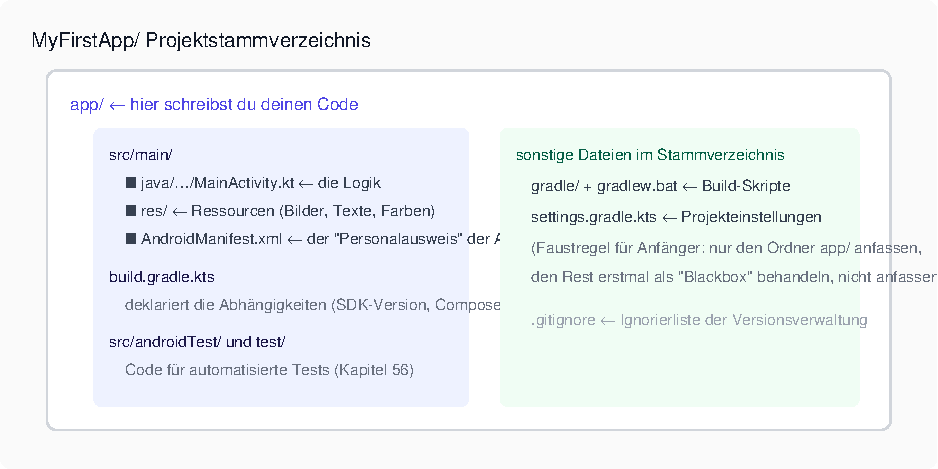
\includegraphics[width=0.92\linewidth]{figures/fig-di-si-shi-jiu-zhang-1}
\\[2pt]\small Abbildung 2: Die Projektstruktur, die Einsteiger kennen müssen (Merkregel: nur den Ordner app/ anfassen)
\end{center}

\begin{itemize}
  \item MainActivity.kt: das "Eingangstor" der App. Tippt der Nutzer auf das Symbol, wird es als erstes geweckt. In der heutigen Vorlage zeigt es "Hello Android!" an.
  \item AndroidManifest.xml: das "Melderegister" der App – hier steht, wie die App heißt, welches Symbol sie hat, welche Seiten es gibt und welche Berechtigungen sie braucht (Kamera, Standort usw.).
  \item res/-Ordner: das Ressourcenlager – hier liegen Bilder, Symbole, Texte, Farben. Texte in Ressourcendateien statt fest im Code zu hinterlegen, ist gute Android-Praxis (Sprach- und Themenwechsel werden so zum Kinderspiel).
  \item build.gradle.kts: das Baurezept – legt die unterstützte Mindestversion fest und welche Bibliotheken eingebunden sind (z. B. Compose).
\end{itemize}

\booksection{Erste Gehversuche: “Hello” durch deinen Namen ersetzen}

Öffne MainActivity.kt und schau dir den von der Compose-Vorlage erzeugten Code an. Finde die Zeile Text(“Hello Android!”) und ersetze den Text in den Anführungszeichen durch deinen Namen, z. B. Text(“Hallo, Max Mustermann! Das ist meine erste App”), und drücke Strg+R (auf dem Mac Cmd+R), um neu zu starten. Ein paar Sekunden später zeigt der Emulator deinen Namen.

\begin{lstlisting}[language=Kotlin]
setContent {
    MyFirstAppTheme {
        Surface(modifier = Modifier.fillMaxSize()) {
            // v hier deinen eigenen Text einsetzen
            Text("Hallo Max! Das ist meine erste App")
        }
    }
}
\end{lstlisting}

Glückwunsch – du hast soeben einen vollständigen Zyklus “Code ändern kompilieren installieren ausführen” hinter dich gebracht. Dieser Zyklus ist der Entwickleralltag der kommenden Tage. Mach gleich weiter: Ändere noch etwas anderes – vergrößere die Schrift, wechsle die Farbe. Im nächsten Kapitel lernst du, woher diese “Magie” kommt.

\booksection{Erste Hilfe bei häufigen Fehlermeldungen: die “Notaufnahme” für die ersten zwei Wochen}

Beim Aufsetzen der Umgebung und beim ersten Build wirst du mit hoher Wahrscheinlichkeit auf die folgenden drei Fehler stoßen. Keine Panik – für alle gibt es ein Gegenmittel:

\begin{center}
\begin{tabularx}{\linewidth}{|X|X|X|}
\hline
\textbf{Fehlerbild} & \textbf{Häufige Ursache} & \textbf{Gegenmittel} \tabularnewline
\hline
Gradle sync failed / Abhängigkeiten laden langsam & Der Zugriff auf die Repositorien über das Netz hakt & Für Gradle einen schnellen Maven-Spiegel einrichten (z. B. Alibaba Cloud oder Tencent Cloud) – suche online nach "gradle china mirror" und richte es nach der Anleitung ein \tabularnewline
SDK-Komponenten fehlen & Der SDK-Download wurde bei der Installation übersprungen & Unter Settings SDK Manager die fehlenden Plattformen und Tools nachinstallieren \tabularnewline
Emulator startet nicht / schwarzer Bildschirm & Virtualisierung nicht aktiviert, Abbild beschädigt & Im BIOS VT-x/AMD-V einschalten; den Emulator löschen und neu anlegen; oder gleich das echte Gerät zum Debuggen nehmen \tabularnewline
\hline
\end{tabularx}
\end{center}

\begin{center}\small\color{gray}Erste-Hilfe-Tabelle für Umgebungsfehler bei Einsteigern\end{center}

\begin{tcbinfo}{Tipp: Wie man Fehlermeldungen richtig sucht}
Die erste Zeile einer Fehlermeldung ist am wertvollsten – kopiere sie wortwörtlich in die Suchmaschine und ergänze das Stichwort “android studio”. Suche nicht nach vagen Fragen wie “Ich bringe meine Umgebung nicht zum Laufen”, sondern nach konkreten Fehlern wie “Gradle sync failed: Could not resolve com.android.tools.build”. Präzise Fragen bringen präzise Antworten.

\end{tcbinfo}

\begin{tcbpractice}{Selbst ausprobieren: Deine "Entwickler-Ritual"-Liste abhaken}
(1) Android Studio installieren und den Emulator zum Laufen bringen; (2) die eigene App einmal auf dem echten Gerät laufen lassen und einen Screenshot als Erinnerung machen; (3) den Hello-Text in deinen Namen ändern; (4) das Projekt zippen und archivieren. Nach diesen vier Schritten darfst du verkünden: Ich bin jetzt auch Android-Entwickler (Screenshot als Beweis).

\end{tcbpractice}

\begin{tcbsummary}{Zusammenfassung des Kapitels}
\begin{itemize}
  \item Android Studio = offizielle, kostenlose IDE; empfohlen: 16 GB RAM + 20 GB Speicher + aktivierte Virtualisierung
  \item Drei Grundzutaten für ein neues Projekt: Name, Paketname (weltweit eindeutig, com.example nicht veröffentlichen), minimale SDK-Version (ab API 26)
  \item Zwei Wege zum Ausführen: Emulator (virtuelles Telefon im Rechner) und echtes Gerät (USB-Debugging einschalten – danach wieder ausschalten)
  \item Projekt-Merkregel: nur den Ordner app/ anfassen – MainActivity.kt ist das Eingangstor, das Manifest das Melderegister, res/ das Ressourcenlager
  \item Entwickleralltag = Code ändern Run Ergebnis ansehen, im Kreis immer wieder
\end{itemize}

\end{tcbsummary}

\bookchapter{Kapitel 50: Kotlin-Schnelleinstieg – die erste Sprache der Android-Entwicklung}

\chapterintro{In diesem Kapitel lernen wir richtig die Sprache. Keine Sorge – Kotlin ist berühmt dafür, einsteigerfreundlich zu sein, und du brauchst kein Grammatikbuch auswendig zu lernen: Mit 20 \% der Syntax verstehst und schreibst du schon 80 \% des Alltagscodes. Den Rest schlägst du nebenbei im Projekt nach. Unser Lernprinzip bleibt: Verstehen schlägt Auswendiglernen, Anwenden schlägt Meisterschaft.}

\booksection{Variablen und Typen: Daten bekommen einen Namen}

Ein Programm ist “Daten + Logik”. Eine Variable gibt den Daten einen Namen und speichert sie. Kotlin kennt zwei Arten der Deklaration:

\begin{lstlisting}[language=Kotlin]
val name = "Max"        // val: schreibgeschützte Variable (standardmäßig empfohlen)
var age = 18             // var: veränderliche Variable (später änderbar)

age = 19                 // <i class="fas fa-check-circle mr-1"></i> var ist änderbar
// name = "Lena"         // <i class="fas fa-times-circle mr-1"></i> val ist nicht änderbar: Kompilierfehler

val score: Int = 100     // der Typ lässt sich auch explizit angeben
val pi = 3.14            // ohne Angabe wird er automatisch abgeleitet
\end{lstlisting}

Die gebräuchlichen Typen lassen sich an einer Hand abzählen – eine Tabelle, und du hast sie:

\begin{center}
\begin{tabularx}{\linewidth}{|X|X|X|}
\hline
\textbf{Typ} & \textbf{Was wird gespeichert?} & \textbf{Beispiel} \tabularnewline
\hline
Int & Ganze Zahl & 42 \tabularnewline
Double & Dezimalzahl & 3.14 \tabularnewline
String & Text & "Hallo" \tabularnewline
Boolean & wahr/falsch & true / false \tabularnewline
List< T> & Eine Sammlung von Daten & listOf(1, 2, 3) \tabularnewline
\hline
\end{tabularx}
\end{center}

\begin{center}\small\color{gray}Die gebräuchlichen Basistypen in Kotlin\end{center}

\begin{tcbinfo}{Tipp: Der val-zuerst-Grundsatz}
Eisernes Gesetz der Kotlin-Community: Standardmäßig val nehmen, var nur, wenn es wirklich nötig ist. Wo val möglich wäre und du var nutzt, mahnt dich die IDE mit gelber Schrift. Diese Gewohnheit erspart dir eine ganze Klasse von Bugs (“Variable wurde unerwartet verändert”) – je weniger sich im Code ändert, desto leichter ist er zu durchschauen.

\end{tcbinfo}

\booksection{Funktionen: Logik zu “Knöpfen” verpacken}

Eine Funktion ist ein Stück Logik mit Namen, wie eine Taste auf der Fernbedienung – einmal drücken (aufrufen), und eine Kette von Aktionen läuft ab. In Kotlin deklariert man sie mit fun:

\begin{lstlisting}[language=Kotlin]
fun greet(name: String): String {
    return "Hallo, $name!"     // das $-Symbol setzt die Variable in den String
}

println(greet("Max"))        // Ausgabe: Hallo Max!

// Einzeiler-Funktionen gehen auch als Ausdruck
fun add(a: Int, b: Int) = a + b

println(add(3, 5))            // Ausgabe: 8
\end{lstlisting}

Ein paar Punkte: Parameter stehen in den Klammern (erst der Name, dann der Typ, getrennt durch Doppelpunkt); der Rückgabetyp steht hinter der Klammer; String-Templates mit \$variablenname sind Kotlins Markenzeichen an Bequemlichkeit – kein mühsames Zusammenkleben von “Zeichenkette + Variable” wie in Java.

\booksection{Bedingungen und Schleifen: Das Programm lernt “denken”}

Die Intelligenz eines Programms kommt von zwei Dingen: es kann entscheiden (if/when) und es kann wiederholen (for/while).

\begin{lstlisting}[language=Kotlin]
// Bedingung: if / else
val age = 17
if (age >= 18) {
    println("Erwachsener")
} else {
    println("Minderjährig")
}

// mehrere Zweige: when (hundertmal besser als switch)
val score = 85
val level = when {
    score >= 90 -> "Hervorragend"
    score >= 60 -> "Ausreichend"
    else -> "Weiter so!"
}

// Wiederholung: for-Schleife
val fruits = listOf("Apfel", "Banane", "Orange")
for (fruit in fruits) {
    println("Ich esse gern $fruit")
}
\end{lstlisting}

when ist die gebräuchlichste Form für mehrere Verzweigungen in Kotlin – in der Android-Entwicklung benutzt du sie täglich (etwa um je nach Zustand unterschiedliche Oberflächen zu zeigen).

\booksection{Null-Sicherheit: Kotlins “Lebensretter”}

Der berühmteste Bug aus dem Java-Zeitalter heißt NullPointerException – das Programm greift auf etwas zu, das “gar nicht da ist”, und stürzt ab. Statistiken zufolge führt diese Ausnahme seit Jahren die Android-Absturz-Charts an. Kotlin löst das Problem auf Sprachebene: Null-Werte sind standardmäßig verboten.

\begin{lstlisting}[language=Kotlin]
var name: String = "Max"   // normaler Typ: darf nie null sein
// name = null                // <i class="fas fa-times-circle mr-1"></i> Kompilierfehler: stoppt dich sofort

var nickname: String? = null // mit Fragezeichen: null erlaubt
nickname = "Tommy"

// bei Nullable-Typen musst du sicher damit umgehen:
println(nickname?.length)    // Safe Call: bei null kommt null zurück, kein Absturz
val len = nickname?.length ?: 0   // Elvis-Operator: Standardwert bei null
println(len)
\end{lstlisting}

\begin{tcbwarn}{Achtung: ? und ?: nicht verwechseln}
String? heißt “darf null sein”, a ?: b heißt “wenn a null ist, nimm b” (die Zeichenkombination sieht aus wie Elvis' Frisur, daher der Name Elvis-Operator). Wenn der Compiler am Anfang über “null-Fehler” meckert, hast du höchstwahrscheinlich vergessen, einen nullable Typ zu behandeln – genau das ist die Sprache, die dich schützt.

\end{tcbwarn}

\booksection{Klassen und Objekte: Die Formen für “Bauteile”}

Die Klasse ist die “Gussform” des Objekts, das Objekt das “Fertigprodukt” der Klasse. Alles in Android – Seiten, Buttons, Daten – sind Objekte. Kotlin hat ein Zauberwerkzeug, die data class (Datenklasse), die speziell zum “Verpacken von Daten” gedacht ist – eine Zeile ersetzt in Java Dutzende:

\begin{lstlisting}[language=Kotlin]
// normale Klasse: die Form
class Dog(val name: String) {
    fun bark() = println("$name: wuff!")
}

val dog = Dog("Rex")      // Objekt erzeugen
dog.bark()                 // Rex: wuff!

// data class: die Daten-Box (mit equals/copy usw. ab Werk)
data class User(val id: Int, val name: String, val email: String)

val me = User(1, "Max", "zhangsan@example.com")
val twin = me.copy(name = "Fritz")   // kopiert und ändert ein Feld
\end{lstlisting}

Wenn du später dein Haushaltsbuch baust, ist jede Buchung eine data class: data class Record(val amount: Double, val category: String, val date: String). Siehst du – du kannst bereits die Code-Struktur eines echten Projekts schreiben.

\booksection{Lambdas und Higher-Order-Funktionen: Kotlins “Syntax-Zucker”}

In Android-Code begegnest du täglich Konstrukten wie \{ ... \} – “Funktionen ohne Namen”, genannt Lambdas (anonyme Funktionen). Button onClick = \{ count++ \} ist ein solches Lambda: “Was nach dem Antippen passiert” wird als Päckchen verpackt und dem Button übergeben.

\begin{lstlisting}[language=Kotlin]
// normaler Weg: eine benannte Funktion definieren und übergeben
fun double(x: Int) = x * 2
val result = listOf(1, 2, 3).map(::double)

// Lambda-Weg: direkt vor Ort definiert, leicht und direkt
val result2 = listOf(1, 2, 3).map { it * 2 }   // it = das aktuelle Element

// filtern + umwandeln hintereinander (in echten Projekten sehr häufig)
val bills = listOf(12.5, 88.0, 5.0, 200.0)
val bigBills = bills.filter { it > 50 }.sorted()
// [88.0, 200.0]——"Rechnungen über 50, sortiert"
\end{lstlisting}

Merke dir ein paar häufige “Sammelkombos”: filter (ausfiltern), map (umformen), sorted (sortieren), sum (aufsummieren). 90 \% deiner künftigen Listenverarbeitung sind Kombinationen dieser vier Züge. Die Kotlin-Philosophie: Was sich in einem Satz sagen lässt, wird niemals in fünf geschrieben.

\booksection{Die Syntax-Spickkarte für Absoluteinsteiger}

Versuche nicht, die ganze Syntax an einem Tag auswendig zu lernen. Speichere diese Karte und schlag beim Schreiben von Code nach – in zwei Wochen sitzt sie von allein:

\begin{center}
\begin{tabularx}{\linewidth}{|X|X|}
\hline
\textbf{Was willst du tun?} & \textbf{Schreibweise} \tabularnewline
\hline
Eine schreibgeschützte Variable definieren & \texttt{val x = 1} \tabularnewline
Eine veränderbare Variable definieren & \texttt{var x = 1} \tabularnewline
Eine Funktion definieren & fun name(parameter): rückgabetyp \{ ... \} \tabularnewline
Entscheiden & if (bedingung) \{...\} else \{...\} \tabularnewline
Mehrere Verzweigungen & when \{ bedingung -> ergebnis \} \tabularnewline
Durchlaufen & for (x in liste) \{ ... \} \tabularnewline
Strings zusammenbauen & "Hallo, \$name" \tabularnewline
Mit null umgehen & \texttt{x?.\allowbreak length ?: 0} \tabularnewline
Eine data class definieren & \texttt{data class X(val a: Int, val b: String)} \tabularnewline
\hline
\end{tabularx}
\end{center}

\begin{center}\small\color{gray}Kotlin-Syntax-Spickkarte (Einsteigerversion)\end{center}

\begin{tcbpractice}{Selbst ausprobieren: Ohne Software-Installation erst mal 10 Minuten Kotlin spielen}
Öffne im Browser play.kotlinlang.org (den offiziellen Kotlin-Online-Spielplatz), füge dort jeden Codeabschnitt aus diesem Kapitel ein und führe ihn aus; ändere Zahlen und Texte und beobachte, wie sich die Ausgabe verändert. Diese 10 Minuten “erst spielen, dann lernen” machen dir den Einstieg in Kapitel 51 doppelt so leicht.

\end{tcbpractice}

\begin{tcbsummary}{Zusammenfassung des Kapitels}
\begin{itemize}
  \item val zuerst, var mit Bedacht; Typen werden automatisch hergeleitet, nach dem Doppelpunkt geht auch explizit
  \item Funktion = verpackte Logik; das String-Template \$ ist das Markenzeichen
  \item if/when zum Entscheiden, for zum Wiederholen; when ist das "Multitalent" der Android-Entwicklung
  \item Null-Sicherheit ist Kotlins Lebensretter: normale Typen lehnen null ab, nullable Typen brauchen ? bzw. ?:
  \item Die data class ist die Schachtel für Daten – ein Feld pro Zeile, im echten Projekt täglich im Einsatz
  \item 20 \% Syntax erledigen 80 \% der Arbeit: erst anwenden, dann meistern
\end{itemize}

\end{tcbsummary}

\bookchapter{Kapitel 51: Oberflächenentwicklung – Einstieg in Jetpack Compose}

\chapterintro{Die Oberfläche ist alles, was der Nutzer sieht. Vor Compose schrieb man Android-Oberflächen in XML – mühsam wie ein Lückentext. 2021 brachte Google Jetpack Compose heraus: Die Oberfläche wird direkt in Kotlin-Code “gemalt”, nach dem Prinzip “was du siehst, ist was du bekommst”, und nach jeder geänderten Zeile aktualisiert sich die Vorschau sofort. 2026 ist Compose der absolute Mainstream für neue Projekte. In diesem Kapitel lernen wir “malen”.}

\booksection{Der Compose-Gedanke: Die Oberfläche ist eine Funktion}

Die Kernidee von Compose in einem Satz: Oberfläche = Funktion. Alles, was auf dem Bildschirm erscheinen kann (Text, Button, Bild), ist eine “Composable-Funktion”, markiert mit @Composable. Verschachtelt man sie wie Bausteine, entsteht die Oberfläche.

\begin{lstlisting}[language=Kotlin]
@Composable
fun Greeting(name: String) {
    Text(text = "Hallo, $name!")     // ein "Text-Baustein"
}

// verschachtelte Komposition: große Blöcke umschließen kleine
@Composable
fun HomeScreen() {
    Column {                          // vertikal gestapelt
        Greeting(name = "Max")
        Greeting(name = "Lena")
        Button(onClick = { /* was beim Klick passieren soll */ }) {
            Text("Klick mich")
        }
    }
}
\end{lstlisting}

Achte auf diesen “Hut” @Composable – er sagt dem Compiler: “Das hier ist ein Oberflächen-Baustein.” Bausteine lassen sich unbegrenzt verschachteln – das ist das ganze Geheimnis von Compose.

\booksection{Grundbausteine: Text, Button, Eingabefeld, Bild}

Die Compose-Komponenten sind “Bausteine” – die vier häufigsten:

\begin{center}
\begin{tabularx}{\linewidth}{|X|X|X|}
\hline
\textbf{Komponente} & \textbf{Wofür gut?} & \textbf{Pflichtparameter} \tabularnewline
\hline
Text & Text anzeigen & text (der anzuzeigende Text) \tabularnewline
Button & Button & onClick (Callback beim Antippen) \tabularnewline
TextField & Eingabefeld & value, onValueChange (Callback bei Eingabeänderung) \tabularnewline
Image & Bild anzeigen & painter (Bildressource) \tabularnewline
\hline
\end{tabularx}
\end{center}

\begin{center}\small\color{gray}Die vier Grundbausteine von Compose\end{center}

\begin{lstlisting}[language=Kotlin]
@Composable
fun BasicWidgets() {
    Column {
        Text(text = "Das ist ein Text")
        Button(onClick = { println("Geklickt!") }) {
            Text("Schaltfläche")
        }
        var input by remember { mutableStateOf("") }
        TextField(
            value = input,
            onValueChange = { input = it },
            label = { Text("Etwas eingeben") }
        )
    }
}
\end{lstlisting}

In den zwei Zeilen des Eingabefelds taucht remember \{ mutableStateOf(“”) \} auf – das ist Composes “Zustands”-Magie, die wir in Abschnitt 5 dieses Kapitels genau anschauen. Fürs Erste reicht es, das Gesicht schon mal kennengelernt zu haben.

\booksection{Das Layout-Trio: Column, Row, Box}

Die Bausteine sind da – aber wie anordnen? Merk dir drei “Schachteln”:

\begin{itemize}
  \item Column: untereinander (wie in der Essensschlange);
  \item Row: nebeneinander (wie nebeneinander sitzen);
  \item Box: übereinander (wie ein Stapel Spielkarten – gut für Badges und Overlays).
\end{itemize}

\begin{lstlisting}[language=Kotlin]
Column {
    Text("Erste Zeile")
    Row {
        Text("Links")
        Text("Rechts")
    }
    Box {
        Text("Unterste Ebene")
        Text("überlagerndes Badge oben")
    }
}
\end{lstlisting}

Soll das Layout hübscher werden? Gib den Komponenten einen Modifier – er schminkt die Bausteine wie mit Make-up:

\begin{lstlisting}[language=Kotlin]
Text(
    text = "Schöner Text",
    modifier = Modifier
        .padding(16.dp)          // Abstand an allen Seiten
        .fillMaxWidth()          // füllt die ganze Breite
        .background(Color.Blue)  // Hintergrundfarbe
        .clickable { /* Klick */ }// klickbar
)
// verkettete Aufrufe: eins nach dem anderen; die Reihenfolge zählt (erst padding, dann Hintergrund; der Hintergrund ohne Rand)
\end{lstlisting}

\begin{tcbwarn}{Achtung: Die Reihenfolge des Modifiers ist entscheidend}
padding(16.dp).background(Blue) und background(Blue).padding(16.dp) wirken unterschiedlich – erstere heißt “erst Abstand, dann Farbe” (der Hintergrund enthält den Abstand nicht), letztere “erst Farbe, dann Abstand” (der Hintergrund schließt den Abstand ein). An genau dieser Stelle malen sich Einsteiger am häufigsten diese “komischen weißen Ränder”. Im Zweifel: vertausche die Reihenfolge, die Vorschau sagt dir sofort die Antwort.

\end{tcbwarn}

\booksection{Zustand: Die Oberfläche zum “Leben” erwecken}

Eine statische Oberfläche ist langweilig. Damit nach einem Tipp auf den Button die Zahl +1 nimmt und man ins Eingabefeld tippen kann, brauchst du einen Zustand (State). Die Compose-Regel: Die Oberfläche spiegelt treu den Zustand wider; ändert sich der Zustand, zeichnet sie sich automatisch neu.

\begin{lstlisting}[language=Kotlin]
@Composable
fun Counter() {
    // remember + mutableStateOf: merkt sich diesen veränderlichen Wert
    var count by remember { mutableStateOf(0) }

    Column {
        Text(text = "Du hast $count Mal geklickt")
        Button(onClick = { count++ }) {   // ändert den Zustand
            Text("Klick +1")                // die Oberfläche aktualisiert sich automatisch
        }
    }
}
\end{lstlisting}

Drei Zeilen Code – ein lebendiger Zähler. Das ist der Vorteil von Compose gegenüber der alten Schreibweise: kein manuelles “Oberfläche aktualisieren” mehr, du änderst nur die Daten. Merk dir zwei Schlüsselfunktionen: remember (der Wert wird bei der Neuzusammensetzung der Oberfläche nicht geleert) und mutableStateOf (sagt Compose: “Dieser Wert hat sich geändert – neu zeichnen”).

Nutzer klickt

Zustand ändert sich (count++)

Compose bemerkt die Änderung

Zeichnet die Oberfläche neu (Recomposition)

\begin{center}\small\color{gray}Abbildung 3: Composes unidirektionaler Datenfluss “Zustand Oberfläche”\end{center}

\booksection{Theme und Dunkelmodus: einmal konfigurieren, überall wirksam}

Das MyFirstAppTheme \{ ... \} im Vorlagenprojekt ist das Theme. Es basiert auf dem Material-3-Designsystem und verwaltet Farben, Schriften und Formen zentral. Den Dunkelmodus zu unterstützen braucht nur drei Schritte:

\begin{enumerate}
  \item Im Theme ein helles/dunkles Farbschema definieren (die Vorlage erzeugt das ColorScheme automatisch);
  \item Wechselt das System in den Dunkelmodus, erkennt das isSystemInDarkTheme() automatisch;
  \item Die vom Theme bereitgestellten Farben verwenden (z. B. MaterialTheme.colorScheme.primary) statt fest kodierte Farbwerte.
\end{enumerate}

\begin{tcbinfo}{Tipp: Material 3 und dynamische Farben}
Ab Android 12 holt sich “Material You” die Farben der App aus deinem Hintergrundbild. Die Compose-Vorlage unterstützt das standardmäßig (dynamicColor). Deine App “zieht sich auf jedem Nutzergerät automatisch um” – das ist die Romantik des modernen Android.

\end{tcbinfo}

\booksection{Vorschau, Animation und Live Edit: Composes “Cheats”}

Drei “Cheats” für das Entwicklungserlebnis – wer sie benutzt hat, will sie nicht mehr missen:

\begin{itemize}
  \item @Preview-Vorschau: Versieh eine Composable mit der Annotation @Preview, und Android Studio rendert die Oberfläche sofort rechts – Code ändern mit Sofortwirkung, ohne jedes Mal auf das Telefon zu installieren;
  \item Live Edit: Das Android Studio von 2026 kann Teile der Änderungen "heiß" auf Emulator/echtem Gerät aktualisieren – kleine Anpassungen wie eine Textfarbe erscheinen sekundenschnell auf dem Gerät;
  \item Animations-APIs: Mit animateFloatAsState und AnimatedVisibility lassen sich mit ein paar Zeilen sanfte Übergänge bauen – der "Hochwertigkeits-Effekt" steckt oft genau in diesen paar Zeilen.
\end{itemize}

\begin{lstlisting}[language=Kotlin]
@Composable
fun AnimatedBox() {
    var big by remember { mutableStateOf(false) }
    // bei Wertänderung sanfter Übergang zum Zielwert
    val size by animateDpAsState(if (big) 120.dp else 60.dp)

    Box(Modifier
        .size(size)
        .background(MaterialTheme.colorScheme.primary)
        .clickable { big = !big }
    )
}
\end{lstlisting}

\begin{tcbinfo}{Tipp: Erst Funktion, dann Animation}
Der klassische Einsteigerfehler: “Die Oberfläche stimmt noch nicht einmal, und schon wird an der Animation gefeilt.” Bringe zuerst die Funktion zum Laufen und lege die Animationen gesammelt ans Ende – auch das ist das Prinzip “Einfachheit zuerst”: Animation ist das i-Tüpfelchen, Funktion ist das Brot.

\end{tcbinfo}

\begin{tcbpractice}{Selbst ausprobieren: Einen "Stimmungs-Button" bauen}
Baue das Vorlagenprojekt in einen Stimmungsschalter um: ein Button, der bei jedem Tipp zwischen fröhlich traurig wütend wechselt; Text und Hintergrundfarbe wechseln mit. Tipp: Wähle Text und Farbe mit when je nach Zustand. Schick das Ergebnis an Freunde und ernte die erste Welle an “Wow, du kannst Apps bauen!”.

\end{tcbpractice}

\begin{tcbsummary}{Zusammenfassung des Kapitels}
\begin{itemize}
  \item Compose-Gedanke: Oberfläche = @Composable-Funktionen, verschachtelt wie Bausteine
  \item Die vier Grundkomponenten: Text / Button / TextField / Image
  \item Das Layout-Trio: Column untereinander, Row nebeneinander, Box gestapelt
  \item Modifier in Kette zum "Schminken": padding, fillMaxWidth, background, clickable – die Reihenfolge hat Bedeutung
  \item Der Zustand ist die Seele: remember + mutableStateOf – Daten ändern, Oberfläche zeichnet neu
  \item Theme mit Material 3 + dynamischen Farben; Dunkelmodus einmal konfigurieren, überall wirksam
\end{itemize}

\end{tcbsummary}

\bookchapter{Kapitel 52: Die vier Grundkomponenten und der Activity-Lebenszyklus}

\chapterintro{Wenn Compose das “Gesicht” der App ist, dann ist dieses Kapitel das “Skelett”. Android kennt vier Grundkomponenten, aus denen jede App zusammengesetzt ist; und die wichtigste davon, die Activity, hat eine “Lebenszyklus-Karte”, die jeder Android-Entwickler ins Gehirn gebrannt haben muss. Nach diesem Kapitel verstehst du so alte Rätsel wie “Warum ist mein App-Zustand weg, wenn ich kurz in den Hintergrund wechsle und zurückkomme?”}

\booksection{Die vier Grundkomponenten: Androids tragende Säulen}

Android definiert offiziell vier Grundkomponenten, die jeweils eine Art von Arbeit übernehmen:

\begin{center}
\begin{tabularx}{\linewidth}{|X|X|X|}
\hline
\textbf{Komponente} & \textbf{Aufgabe} & \textbf{Zum Vergleich} \tabularnewline
\hline
Activity & Eine sichtbare Oberfläche & Die Schaufensterfront des Ladens – sichtbar und bedienbar \tabularnewline
Service & Der "Unsichtbare", der im Hintergrund schuftet & Der Lagerarbeiter – Musik abspielen, Dateien herunterladen, ganz ohne Oberfläche \tabularnewline
BroadcastReceiver & System-Broadcasts empfangen & Die Pförtnerloge – der Lautsprecher für "Akku ist leer" und "Netz ist weg" \tabularnewline
ContentProvider & Daten app-übergreifend teilen & Der öffentliche Aktenschrank – z. B. Kontakte für andere Apps freigeben \tabularnewline
\hline
\end{tabularx}
\end{center}

\begin{center}\small\color{gray}Die vier Grundkomponenten von Android auf einen Blick\end{center}

Als Einsteiger verbringst du 95 \% deiner Zeit mit der Activity; Service und BroadcastReceiver brauchst du für Musikwiedergabe und Push-Nachrichten; ContentProvider nutzt du am seltensten (das System kapselt die gebräuchlichen Daten bereits). Und beachte: Alle vier Komponenten müssen sich im AndroidManifest.xml “anmelden” – ohne Registrierung findet das System sie nicht.

\booksection{Der Activity-Lebenszyklus: die erste “Schatzkarte” der Android-Entwicklung}

Eine App auf dem Telefon kann jederzeit unterbrochen werden: Ein Anruf kommt, der Nutzer wechselt kurz zu WeChat, das System beendet dich wegen Speichermangels … Das Leben einer Activity ist eine Rundreise auf dieser Karte:

onCreate (Geburt: Initialisierung)

onStart (sichtbar)

onResume (im Vordergrund aktiv)

onPause (teilweise verdeckt)

onStop (ganz unsichtbar)

onDestroy (zerstört)

onRestart / onStart / onResume: beim Zurückkehren in den Vordergrund umgekehrt

\begin{center}\small\color{gray}Abbildung 4: Der Activity-Lebenszyklus (vorwärts: obere Reihe Geburt untere Reihe Abschied; auf dem Rückweg genau umgekehrt)\end{center}

\begin{center}
\begin{tabularx}{\linewidth}{|X|X|X|}
\hline
\textbf{Callback} & \textbf{Wann wird er ausgelöst?} & \textbf{Typischer Einsatz} \tabularnewline
\hline
onCreate & Beim Erzeugen der Activity (einmal) & Oberfläche laden, Daten initialisieren \tabularnewline
onStart & Die Oberfläche wird sichtbar & Ein wenig leichtgewichtige Logik starten \tabularnewline
onResume & Hat den Fokus, ist bedienbar & Animationen starten, Wiedergabe fortsetzen \tabularnewline
onPause & Teilweise verdeckt oder im Begriff, verlassen zu werden & Animationen pausieren, Entwurf speichern \tabularnewline
onStop & Vollständig unsichtbar & Schwere Ressourcen freigeben, Downloads pausieren \tabularnewline
onDestroy & Unmittelbar vor dem Entfernen & Die letzten Aufräumarbeiten \tabularnewline
\hline
\end{tabularx}
\end{center}

\begin{center}\small\color{gray}Typische Einsätze der sechs Lifecycle-Callbacks\end{center}

\textbf{Stolperfalle: Eine Drehung des Bildschirms “tötet” die Activity}\par

Der klassischste Stolperstein: Man dreht den Bildschirm, und der ganze Text im Eingabefeld ist weg. Grund: Eine Bildschirmdrehung zerstört die Activity standardmäßig und baut sie neu auf (durchlaufen von onDestroy onCreate). Lösung: Den Zustand mit rememberSaveable sichern (in Compose der Ersatz für remember) – es holt die Werte beim Neuaufbau automatisch zurück. In den Kapiteln 6 und 7 wirst du es immer wieder brauchen.

\booksection{Intent: das “Ticket” für den Verkehr in der App und nach außen}

Der Intent (die “Absicht”) ist das “Fahrticket” für die Kommunikation zwischen Komponenten. Ob du von einer Seite zur anderen springen, den Browser öffnen oder die Kamera aufrufen willst – immer musst du “ein Ticket lösen und einsteigen”:

\begin{lstlisting}[language=Kotlin]
// Variante 1: expliziter Intent – klar angegeben, zu welcher Seite
val intent = Intent(this, DetailActivity::class.java)
intent.putExtra("name", "Max")     // nimmt "Gepäck" mit (die Daten)
startActivity(intent)

// Variante 2: impliziter Intent – du sagst nur, was zu tun ist; das System sucht, wer es tut
val web = Intent(Intent.ACTION_VIEW, Uri.parse("https://developer.android.com"))
startActivity(web)   // das System öffnet den Browser (oder lässt dich wählen)
\end{lstlisting}

Beide Varianten haben ihren Zweck: Explizit für Seitensprünge innerhalb der eigenen App; implizit, um Fähigkeiten des Systems oder anderer Apps zu nutzen (Webseite öffnen, anrufen, teilen). In Compose-Projekten holst du in einer Composable mit LocalContext.current den Context und kannst dann startActivity aufrufen.

\booksection{Mehrere Seiten und Navigation}

Echte Apps haben mehrere Seiten. Die offiziell empfohlene Navigationslösung für Compose ist Navigation Compose (Bibliothek androidx.navigation):

\begin{lstlisting}[language=Kotlin]
val navController = rememberNavController()

NavHost(navController, startDestination = "home") {
    composable("home") { HomeScreen(navController) }
    composable("detail/{name}") { entry ->
        val name = entry.arguments?.getString("name")
        DetailScreen(name ?: "Unbekannt")
    }
}

// um innerhalb der Ansicht zu navigieren:
navController.navigate("detail/Max")     // mit Parameter
navController.popBackStack()              // zurück zur vorherigen Seite
\end{lstlisting}

\begin{tcbinfo}{Tipp: Und wenn es zu viele Seiten werden?}
Sobald das Projekt wächst, schreib alle Seitenrouten gebündelt in eine Datei (z. B. AppNavGraph.kt) und verwalte sie zentral – lass die Logik “Wohin springe ich?” nicht auf alle Seiten verstreuen. Das ist der erste Schritt von “läuft irgendwie” zu “wartbar”.

\end{tcbinfo}

\booksection{Nebenbei erklärt: Was ist ein Fragment (und warum lehrt dieses Buch es nicht)}

In alten Tutorials wirst du unweigerlich auf Fragment stoßen – einen “wiederverwendbaren Oberflächen-Schnipsel” innerhalb einer Activity, in der alten Mehrseiten-Architektur der absolute Star. Im Compose-Zeitalter reichen aber Composable-Funktionen + Navigation-Routen für Seiten, und auch offiziell ist Fragment zurückgestuft worden. Deshalb taucht es in diesem Buch nicht im Hauptweg auf.

Mein Rat: In neuen Projekten Fragment nicht aktiv einsetzen; aber wenn du alten Code liest oder im Vorstellungsgespräch danach gefragt wirst, reicht zu wissen: “Ein Fragment ist ein Oberflächen-Schnipsel, das in einer Activity steckt.” Lernmaterialien immer bevorzugt ab 2023 wählen – die “alten Kalenderblätter” des Android-Stacks veralten schneller, als man denkt.

\begin{tcbpractice}{Selbst ausprobieren: Dem Zähler ein "Gedächtnis" verpassen}
Bau den Zähler aus Kapitel 51 um: (1) Ersetze remember durch rememberSaveable und prüfe nach einer Bildschirmdrehung, ob die Zahl überlebt hat; (2) füge einen “Über”-Button hinzu, der mit Navigation auf eine zweite Seite springt und dort die Versionsnummer zeigt; (3) lass in onCreate bzw. onPause beider Seiten Logausgaben schreiben (Log.d) und beobachte in Logcat die Reihenfolge der Lifecycle-Aufrufe. Nach diesen drei Schritten ist der Lebenszyklus keine Theorie mehr.

\end{tcbpractice}

\begin{tcbsummary}{Zusammenfassung des Kapitels}
\begin{itemize}
  \item Die vier Grundkomponenten: Activity (Schaufenster), Service (Hintergrund), BroadcastReceiver (Lautsprecher), ContentProvider (Aktenschrank)
  \item Sechs Lifecycle-Callbacks: onCreate onStart onResume onPause onStop onDestroy
  \item Eine Bildschirmdrehung zerstört die Activity und baut sie neu: Mit rememberSaveable den Zustand retten
  \item Intent ist das "Ticket": explizit zur eigenen Seite, implizit für System-Fähigkeiten
  \item Mehrere Seiten mit Navigation Compose: NavHost + composable-Routen
\end{itemize}

\end{tcbsummary}

\bookchapter{Kapitel 53: Datenspeicherung und Netzwerkanfragen}

\chapterintro{Eine App, die nur “angucken” kann, ist tot; erst eine App, die Daten speichern und sich vernetzen kann, lebt. In diesem Kapitel lernst du das “Trio” der Android-Datenschicht kennen: DataStore (kleine Einstellungen speichern), Room (strukturierte Daten speichern), Retrofit (mit dem Server sprechen) – plus ihr “Dispositionszentrum”, die Koroutinen. Nach diesem Kapitel kannst du echte Apps schreiben, die sich Nutzer-Gewohnheiten merken und Inhalte live aktualisieren.}

\booksection{Welches Speicherkonzept wofür? Erst diese Tabelle anschauen}

\begin{center}
\begin{tabularx}{\linewidth}{|X|X|X|X|}
\hline
\textbf{Konzept} & \textbf{Wofür geeignet?} & \textbf{Eigenschaften} & \textbf{Wo im Buch genutzt?} \tabularnewline
\hline
DataStore & Verstreute Einstellungen (Theme, Schalter) & Schlüssel-Wert-Paare, einfach und sicher & Kapitel 54: Einstellungen des Haushaltsbuchs \tabularnewline
Room & Strukturierte Daten (Buchungen, Nutzer) & Eine echte SQLite-Datenbank verpackt, abfragbar & Kapitel 54: Buchungseinträge \tabularnewline
Retrofit & Serverdaten (nicht speichern, online abrufen) & Der De-facto-Standard unter den HTTP-Bibliotheken & Kapitel 55: Wetterdaten \tabularnewline
\hline
\end{tabularx}
\end{center}

\begin{center}\small\color{gray}Die Arbeitsteilung des Daten-Trios\end{center}

Merksatz: “Kleine Einstellungen ins DataStore, Daten in Mengen ins Room, Daten von draußen über Retrofit.” Das in alten Tutorials allgegenwärtige SharedPreferences ist von DataStore abgelöst, handgeschriebenes SQLite-SQL von Room – lern gleich das Neue, geh nicht den alten Weg.

\booksection{DataStore: Kleine Einstellungen wegspeichern}

Werte wie “die zuletzt gewählte Währung” oder “ist der Dunkelmodus an?” willst du verstreut abspeichern – dafür ist DataStore (Preferences-Variante) da:

\begin{lstlisting}[language=Kotlin]
val Context.dataStore by preferencesDataStore(name = "settings")

// schreiben: Wert speichern
suspend fun saveTheme(isDark: Boolean) {
    context.dataStore.edit { prefs ->
        prefs[THEME_KEY] = isDark
    }
}

// lesen: herausholen (Flow meldet Änderungen automatisch)
val themeFlow: Flow<Boolean> = context.dataStore.data
    .map { it[THEME_KEY] ?: false }
\end{lstlisting}

Achte darauf: Zurückgegeben wird ein Flow – ein Datenstrom, der “fließt”. Sobald sich der Wert ändert, bekommen alle Stellen, die ihn beobachten, automatisch den neuen Wert. Dieses Konzept (Reaktivität) ist der Grundstein des modernen Android – in Kapitel 54 kommt es zum Praxiseinsatz.

\booksection{Room: Den Daten ein “richtiges Zuhause” geben}

Ein Haushaltsbuch hat hunderte, tausende Buchungen, die nach Kategorie und Monat abgefragt und ausgewertet werden sollen – dafür braucht es eine Datenbank. Room ist die offizielle Hülle um SQLite und macht “Tabellen anlegen, Daten abfragen” so natürlich wie Kotlin-Schreiben. Drei Dinge:

\begin{lstlisting}[language=Kotlin]
// 1. Entity: die Tabellenstruktur (eine Tabelle = eine Data Class)
@Entity(tableName = "records")
data class Record(
    @PrimaryKey(autoGenerate = true) val id: Long = 0,
    val amount: Double,
    val category: String,
    val note: String,
    val date: String
)

// 2. Dao: das Operations-Interface (anlegen, löschen, ändern, lesen)
@Dao
interface RecordDao {
    @Query("SELECT * FROM records ORDER BY date DESC")
    fun getAll(): Flow<List<Record>>

    @Insert
    suspend fun insert(record: Record)

    @Delete
    suspend fun delete(record: Record)

    @Query("SELECT SUM(amount) FROM records WHERE category = :c")
    suspend fun sumByCategory(c: String): Double
}

// 3. Database: die Endmontage
@Database(entities = [Record::class], version = 1)
abstract class AppDatabase : RoomDatabase() {
    abstract fun recordDao(): RecordDao
}
\end{lstlisting}

Dieses “Trio”-Template kannst du unverändert in jedes deiner Projekte übernehmen – einfach die Feldnamen austauschen. Die Abfragen liefern Flow, die Oberfläche aktualisiert sich automatisch mit den Daten – herrlich.

\booksection{Retrofit: Mit dem Server sprechen}

Wetter, Nachrichten, Wechselkurse … Diese Daten liegen nicht auf dem Telefon, sondern auf den Servern von anderen. Retrofit macht “Daten vom Server anfordern” so einfach wie einen Funktionsaufruf. In drei Schritten:

\begin{lstlisting}[language=Kotlin]
// 1. Interface definieren: HTTP-Anfragen als Funktionen beschreiben
interface WeatherApi {
    @GET("v1/weather")
    suspend fun getWeather(@Query("city") city: String): WeatherResponse
}

// 2. Instanz erzeugen
val api = Retrofit.Builder()
    .baseUrl("https://api.example.com/")
    .addConverterFactory(GsonConverterFactory.create())
    .build()
    .create(WeatherApi::class.java)

// 3. aufrufen wie eine Funktion (in einer Koroutine)
val result = api.getWeather("Berlin")
\end{lstlisting}

\textbf{Stolperfalle: Zwei eiserne Netzwerk-Regeln}\par

(1) Netzwerkanfragen dürfen niemals im Hauptthread laufen – die Oberfläche friert ein oder die App stürzt ab (NetworkOnMainThreadException). Alle Netzwerkaufrufe gehören in eine Koroutine (viewModelScope.launch). (2) Klartext-HTTP ist standardmäßig verboten: Ab Android 9 wird HTTPS verlangt. Für Tests mit lokalen http://-Adressen musst du im Manifest usesCleartextTraffic explizit deklarieren – ein echtes Produkt muss aber komplett über HTTPS laufen.

\booksection{JSON-Parsen: Den Netzdaten eine “Übersetzung” geben}

Was der Server zurückgibt, ist meist JSON – ein Text wie ein “verschachteltes Wörterbuch”. Retrofit braucht einen “Dolmetscher”, der daraus Kotlin-Objekte macht. 2026 gibt es zwei Mainstream-Lösungen:

\begin{center}
\begin{tabularx}{\linewidth}{|X|X|X|}
\hline
\textbf{Konzept} & \textbf{Eigenschaften} & \textbf{Empfohlen für} \tabularnewline
\hline
Gson / Moshi & Der klassische Reflection-Ansatz, null Konfigurationsaufwand & Schneller Start, kleine Projekte mit wenigen Feldern \tabularnewline
kotlinx.serialization & Die offizielle Lösung zur Compiler-Zeit, schneller und sicherer & Erste Wahl für neue Projekte (2026er Mainstream) \tabularnewline
\hline
\end{tabularx}
\end{center}

\begin{center}\small\color{gray}Die beiden großen JSON-Lösungen\end{center}

\begin{lstlisting}[language=Kotlin]
// versieh die Data Class mit @Serializable
@Serializable
data class WeatherResponse(
    val weather: List<Weather>,
    val main: Main,
    val name: String
)

// Retrofit bekommt den passenden Converter angehängt (Beispiel mit offizieller Unterstützung ab Retrofit 2.11+):
// .addConverterFactory(json.asConverterFactory("application/json".toMediaType()))
\end{lstlisting}

Gleich welche Lösung – das eiserne Gesetz lautet: Erst das echte zurückgegebene JSON anschauen, dann die Felder definieren. Viele “Parsen fehlgeschlagen”-Bugs entstehen, weil Feldnamen verschrieben oder Verschachtelungsebenen falsch geraten sind – gib das rohe JSON aus und gleiche ab, in zehn Sekunden ist der Fehler geortet.

\booksection{Koroutinen: Die “Gemeinsprache” der Android-Concurrency}

\booksection{Koroutinen: Die “Gemeinsprache” der Android-Concurrency}

Das immer wieder auftauchende suspend und launch stammen aus den Kotlin-Koroutinen – der offiziellen Concurrency-Lösung von Android. Grob gesagt: Operationen, die “ein Weilchen dauern” (Netzwerk, Datenbank), blockieren die Oberfläche nicht.

\begin{lstlisting}[language=Kotlin]
// starte eine Koroutine im ViewModel
viewModelScope.launch {
    val records = dao.getAll().first()  // suspend: hält automatisch an und wartet
    // Zustand der Oberfläche aktualisieren …
}

// Spickzettel der Schlüsselwörter:
// suspend   —— "ich muss warten, halte andere nicht auf"
// launch    —— "auf geht's!"
// viewModelScope —— die "Werkstatt", die der Ansicht folgt; räumt sich beim Zerstören selbst ab
\end{lstlisting}

Als Einsteiger musst du zunächst nur die Anwendung kennen; das Prinzip dahinter (“Anhalten und Fortsetzen”) kannst du später vertiefen. 90 \% dessen, was du im Alltag schreibst, ist diese eine Schablone.

\begin{tcbpractice}{Selbst ausprobieren: Eine kleine App "Satz des Tages" bauen}
Such dir eine kostenlose Zitate-API (z. B. hitokoto o. Ä.), hole mit Retrofit den “Satz des Tages” und zeige ihn mitten auf dem Bildschirm; füge einen Button “Noch einen” hinzu (neue Anfrage in einer Koroutine). Speichere Lieblingssätze mit Room in eine “Favoriten”-Sammlung. Diese Übung nutzt DataStore/Room/Retrofit/Korouten je einmal – danach sind Kapitel 7 und 8 ein Kinderspiel.

\end{tcbpractice}

\begin{tcbsummary}{Zusammenfassung des Kapitels}
\begin{itemize}
  \item Merksatz: kleine Einstellungen ins DataStore, Daten in Mengen ins Room, Daten von draußen über Retrofit
  \item DataStore liefert Flow: Ändert sich der Wert, bekommen Beobachter ihn automatisch
  \item Room-Trio: @Entity (Tabelle) + @Dao (Operationen) + @Database (Endmontage) – die Schablone ist direkt wiederverwendbar
  \item Retrofit in drei Schritten: Interface definieren Instanz erzeugen in der Koroutine aufrufen
  \item Zwei eiserne Regeln: Netzwerk nie im Hauptthread; echte Produkte immer über HTTPS
  \item Koroutine = Warten, ohne die Oberfläche zu blockieren; viewModelScope ist die eigene Werkstatt jeder Seite
\end{itemize}

\end{tcbsummary}

\bookchapter{Kapitel 54: Projekt 1 – Mein Haushaltsbuch (Lokalversion)}

\chapterintro{Willkommen bei deinem ersten “richtigen Projekt”. Dieses Haushaltsbuch geht zwar nicht ins Netz, aber es hat alles, was dazugehört: eine Buchung erfassen, den Verlauf ansehen, monatliche Auswertungen, Löschen und Ändern. Wenn du fertig bist, hast du den kompletten Ablauf “Daten Logik Oberfläche” einmal durchlaufen. Und: Nicht sofort den Code abschreiben – erst klar denken, dann anpacken. Das ist unser Prinzip von Anfang an.}

\booksection{Über die Anforderungen nachdenken: erst fünf Fragen stellen}

Bevor du loslegst, sortiere deine Idee mit den “fünf Anforderungsfragen”:

\begin{center}
\begin{tabularx}{\linewidth}{|X|X|}
\hline
\textbf{Frage} & \textbf{Antwort} \tabularnewline
\hline
Who (für wen?) & Für dich selbst, auch für Familie und Freunde \tabularnewline
What (was?) & Einnahmen und Ausgaben erfassen, Verlauf ansehen, monatliche Summen, Auswertung nach Kategorien \tabularnewline
Why (warum?) & Übung + herausfinden, wohin das Geld fließt \tabularnewline
How (wie?) & Kotlin + Compose + Room + MVVM, rein lokal ohne Backend \tabularnewline
Constraint (Rahmenbedingung) & In einer Woche fertig; mindestens Android 8 unterstützen; auch ohne Store-Veröffentlichung nach Store-Maßstab schreiben \tabularnewline
\hline
\end{tabularx}
\end{center}

\begin{center}\small\color{gray}Die fünf Anforderungsfragen des Haushaltsbuchs\end{center}

Dann zerlegst du es in kleine Schritte, von denen jeder einzeln “benutzbar” ist: (1) Room-Datenschicht bauen (eine Buchung speichern können); (2) Listenseite (Verlauf ansehen können); (3) Erfassungsseite (Buchung hinzufügen können); (4) Löschen und Bearbeiten; (5) Monats-Karte. Nach jedem Schritt ist die App ein “brauchbares Ding”.

\booksection{Die Datenschicht: Den “Buchungen” ein Zuhause geben}

Definiere zuerst, wie eine Buchung aussieht – die Felder sollen reichen, aber nicht gierig sein:

\begin{lstlisting}[language=Kotlin]
@Entity(tableName = "records")
data class Record(
    @PrimaryKey(autoGenerate = true) val id: Long = 0,
    val type: String,        // "income" Einnahme | "expense" Ausgabe
    val amount: Double,      // Betrag (Yuan)
    val category: String,    // Kategorie: Essen, Verkehr, Gehalt …
    val note: String = "",   // Notiz (optional)
    val date: String         // "2026-08-15"
)
\end{lstlisting}

In den Dao kommen zwei “Statistik-Abfragen” – sie sind die Seele des Haushaltsbuchs:

\begin{lstlisting}[language=Kotlin]
@Dao
interface RecordDao {
    @Query("SELECT * FROM records ORDER BY date DESC, id DESC")
    fun getAll(): Flow<List<Record>>

    @Insert
    suspend fun insert(record: Record)

    @Delete
    suspend fun delete(record: Record)

    @Query("SELECT COALESCE(SUM(amount),0) FROM records WHERE type='income' AND date LIKE :month || '%'")
    suspend fun monthIncome(month: String): Double   // month hat das Format "2026-08"

    @Query("SELECT COALESCE(SUM(amount),0) FROM records WHERE type='expense' AND date LIKE :month || '%'")
    suspend fun monthExpense(month: String): Double
}
\end{lstlisting}

\begin{tcbinfo}{Tipp: Warum Double für Beträge?}
Seriöse Finanz-Apps nutzen BigDecimal oder “Int in Cent”, um Rundungsfehler zu vermeiden (das alte Problem 0,1+0,2$\neq$0,3). Für ein Übungsprojekt reicht Double völlig; baust du eines Tages ein echtes Finanzprodukt, rechne in Cent – eine Falle, in die unzählige Vorgänger getreten sind.

\end{tcbinfo}

\booksection{MVVM: Oberfläche und Logik ziehen getrennte Wege}

Die Oberfläche direkt auf die Datenbank zugreifen lassen? Läuft zwar – aber der Oberflächen-Code wird lang und furchtbar. Die MVVM-Architektur lässt jeden seine Rolle spielen: View (Oberfläche) zeichnet nur, ViewModel (Logikzentrale) verwaltet die Daten, Model (Room) kümmert sich um die Speicherung.

View (Compose-Oberfläche)

ViewModel (Zustand und Logik)

Model (Datenlayer mit Room)

\begin{center}\small\color{gray}Abbildung 5: Die drei MVVM-Schichten – Daten fließen in eine Richtung, keine Schicht greift über\end{center}

\begin{lstlisting}[language=Kotlin]
class RecordViewModel(private val dao: RecordDao) : ViewModel() {

    // wandelt den Flow in einen von der UI beobachtbaren Zustand
    val records = dao.getAll()
        .stateIn(viewModelScope, SharingStarted.WhileSubscribed(), emptyList())

    // Nutzeraktionen: suspend-Funktionen aufrufen
    fun addRecord(type: String, amount: Double, category: String, note: String, date: String) {
        viewModelScope.launch {
            dao.insert(Record(type = type, amount = amount,
                category = category, note = note, date = date))
        }
    }

    fun deleteRecord(record: Record) {
        viewModelScope.launch { dao.delete(record) }
    }
}
\end{lstlisting}

In der Oberfläche (Compose) so: val vm: RecordViewModel = viewModel(), dann val list by vm.records.collectAsState() – sobald sich die Daten ändern, aktualisiert sich die Liste von selbst, du musst nichts tun. Das ist die geballte Kraft von MVVM + Flow + Compose.

\booksection{Oberfläche: Listenseite + Erfassungsseite}

Für die Listenseite nimm LazyColumn (träge ladende Liste) – selbst bei riesigen Datenmengen ruckelt nichts:

\begin{lstlisting}[language=Kotlin]
@Composable
fun RecordListScreen(vm: RecordViewModel) {
    val records by vm.records.collectAsState()

    Column {
        // oben die Zusammenfassungs-Karte (Einnahmen - Ausgaben = Saldo)
        SummaryCard(records)

        // Liste der Buchungen
        LazyColumn {
            items(records, key = { it.id }) { record ->
                RecordRow(record) { vm.deleteRecord(record) }
            }
        }

        // schwebender Button "Ausgabe erfassen"  öffnet den Eingabedialog
        FloatingActionButton(onClick = { showAddDialog = true }) {
            Text("+")
        }
    }
}

@Composable
fun RecordRow(record: Record, onDelete: () -> Unit) {
    Row(Modifier.fillMaxWidth().padding(12.dp)) {
        Text(record.category, fontWeight = FontWeight.Bold)
        Spacer(Modifier.weight(1f))
        Text(if (record.type == "income") "+${record.amount}" else "-${record.amount}",
             color = if (record.type == "income") Color(0xFF27AE60) else Color(0xFFC0392B))
    }
}
\end{lstlisting}

Zum Erfassen ist ein AlertDialog am bequemsten: ein paar Eingabefelder + Umschalter Einnahme/Ausgabe + Kategorie-Dropdown, und bei “OK” rufst du vm.addRecord(...) auf.

\begin{tcbwarn}{Achtung: Bei der Eingabeprüfung nicht faulenzen}
Das Betragsfeld musst du unbedingt prüfen: Leere Werte, Negativeingaben, “abc” und Ähnliches sind abzufangen (mit toDoubleOrNull() prüfen). Einer der häufigsten Gründe für App-Abstürze ist, “die Eingaben des Nutzers für brav zu halten”. Merke: Behandle alles, was Nutzer eintippen, wie etwas, das du feindlich prüfen musst.

\end{tcbwarn}

\booksection{Bearbeiten und Löschen: Daten müssen “rein und raus” können}

Ein Haushaltsbuch, das nur hinzufügen kann, ist nach drei Tagen unbrauchbar. Zwei Operationen noch:

\begin{lstlisting}[language=Kotlin]
// zwei Methoden im Dao ergänzen:
@Query("UPDATE records SET amount=:amount, category=:category, note=:note WHERE id=:id")
suspend fun update(id: Long, amount: Double, category: String, note: String)

@Query("DELETE FROM records WHERE id=:id")
suspend fun deleteById(id: Long)

// in der Oberfläche: langes Tippen auf einen Eintrag öffnet das Menü "Bearbeiten/Löschen" (in Compose: DropdownMenu oder AlertDialog)
// vor dem Löschen besser einen Bestätigungsdialog: "versehentliches Löschen" ist, was Nutzer von Ausgaben-Apps am meisten hassen
\end{lstlisting}

Zwei Erfahrungsregeln für die Bedienung: Beim Löschen immer eine zweite Bestätigung (gegen Versehen), beim Bearbeiten möglichst die Originalwerte voreintragen (ein Zeichen ändern ist leichter als alles neu tippen). Unterschätz diese Details nicht – “Produktgefühl” besteht genau aus solchen Details.

\booksection{Abnahme: drei Prüfebenen + zwei Fortgeschrittenen-Herausforderungen}

\booksection{Abnahme: drei Prüfebenen + zwei Fortgeschrittenen-Herausforderungen}

Wenn das Projekt fertig ist, nimm die Abnahme in drei Ebenen vor: “Funktion Grenzfälle Architektur”: Kannst du erfassen? Löschen? Sind die Daten nach einem Neustart noch da (Funktion)? Stürzt die App bei Betrag 0 oder negativ ab? Gehen bei einer Bildschirmdrehung Daten verloren (Grenzfälle)? Sind Oberfläche und Daten sauber getrennt, sind Felder hart kodiert (Architektur)?

Nach bestandener Basis-Abnahme gönn dir zwei “Fortgeschrittenen-Gerichte”:

\begin{enumerate}
  \item Monatsfilter: oben einen Monatswechsel ergänzen (z. B. 2026-08 v), die Liste zeigt nur den Verlauf des jeweiligen Monats;
  \item Kreisdiagramm nach Kategorien: mit Composes Canvas oder einer leichten Chart-Bibliothek "wohin das Geld fließt" als Tortendiagramm zeichnen – danach sieht das Haushaltsbuch schon richtig nach Produkt aus.
\end{enumerate}

\begin{tcbpractice}{Selbst ausprobieren: Diese Woche fertigstellen}
Arbeite in der Reihenfolge “Datenschicht ViewModel Listenseite Erfassungsseite Auswertungskarte”, jeden Tag ein Schritt. Wenn du festhängst, wirf die Fehlermeldung wörtlich in die Suchmaschine oder an eine KI (erinnerst du dich an Teil 7, “AI-Programmierung in der Praxis”? Beschreibe das Problem mit “erwartetes Verhalten, tatsächliches Verhalten, Schritte zur Reproduktion”). Wenn du fertig bist, führe eine Woche lang damit Buch – eine selbstgebaute App im eigenen Einsatz gibt dir Schwung für den weiteren Weg.

\end{tcbpractice}

\begin{tcbsummary}{Zusammenfassung des Kapitels}
\begin{itemize}
  \item Fünf Anforderungsfragen zerlegen in Schritte, von denen jeder einzeln funktioniert – dann loslegen
  \item Datenschicht: Record-Entity + Dao (inkl. SQL für Monatsstatistik) + Database
  \item MVVM-Arbeitsteilung: View zeichnet nur, ViewModel steuert die Logik, Model verwaltet die Speicherung
  \item Flow + stateIn + collectAsState: Daten ändern sich, die Oberfläche aktualisiert sich automatisch
  \item LazyColumn als träge ladende Liste; AlertDialog für die Erfassung
  \item Abnahme in drei Ebenen (Funktion/Grenzfälle/Architektur) + Zusatzaufgaben (Monatsfilter, Kreisdiagramm)
\end{itemize}

\end{tcbsummary}

\bookchapter{Kapitel 55: Projekt 2 – Wetter-App (Netzversion)}

\chapterintro{Das Haushaltsbuch trainiert die “inneren Kräfte”, die Wetter-App zeigt dir die “große Welt” – sie verkehrt mit dem Internet. In diesem Projekt lernst du: eine kostenlose API beantragen, JSON parsen, drei Oberflächenzustände (“lädt/erfolgreich/gescheitert”) behandeln und den API-Schlüssel gut verstecken. Danach kannst du jede beliebige “Online-App” bauen – Nachrichten, Wechselkurse, Übersetzung, immer dasselbe Rezept.}

\booksection{Eine kostenlose Wetter-API beantragen}

Zum Üben empfehle ich OpenWeatherMap oder QWeather (Hefeng Weather) – beide haben kostenlose Kontingente, registrieren und loslegen. Am Beispiel OpenWeatherMap:

\begin{enumerate}
  \item Konto registrieren auf der Seite API keys einen Key erzeugen (apikey);
  \item Die kostenlose Version darf die Schnittstelle Current Weather (aktuelles Wetter) aufrufen: api.openweathermap.org/data/2.5/weather? q=beijing\&appid=deinKey\&units=metric;
  \item Probier sie erst einmal im Browser aus und schau an, wie das zurückgegebene JSON aussieht – diese "Vorbereitung" ist Pflicht, bevor du irgendeine API anbindest.
\end{enumerate}

\textbf{Stolperfalle: Der Schlüssel darf niemals fest im Code stehen}\par

Ein API-Key ist quasi dein “Wallet-Passwort” – landet er im Code und wird nach GitHub gepusht, spinnen ihn Crawler binnen Stunden auf und missbrauchen ihn. Richtig: Ab in local.properties (diese Datei ist über gitignore bereits ignoriert) und von dort über Gradles buildConfig in den Code einlesen. Suche nach “Best Practices Android API Key verstecken” und richte es entsprechend ein.

\booksection{Die Netzwerkschicht: Retrofit + JSON-Parsen}

Definiere zuerst das “Datenmodell” nach dem JSON, das die API zurückgibt; alles, was kein Gegenstück hat, wird ignoriert:

\begin{lstlisting}[language=Kotlin]
// JSON: {"weather":[{"description":"Klar"}],"main":{"temp":26.5,"humidity":40},"name":"Berlin"}
data class WeatherResponse(
    val weather: List<Weather>,
    val main: Main,
    val name: String
)
data class Weather(val description: String)
data class Main(val temp: Double, val humidity: Int)

interface WeatherApi {
    @GET("data/2.5/weather")
    suspend fun getWeather(
        @Query("q") city: String,
        @Query("appid") key: String,
        @Query("units") metric: String = "metric",
        @Query("lang") lang: String = "zh_cn"
    ): WeatherResponse
}
\end{lstlisting}

Gson stopft das JSON automatisch in diese data classes – stimmen die Feldnamen, passiert die Magie von ganz allein.

\booksection{Drei Oberflächenzustände: lädt / erfolgreich / gescheitert}

Die Seele einer Online-App ist das “Zustandsmanagement”. Langsames Netz, keine Verbindung, falsch geschriebener Stadtname … Für jeden Fall braucht die Oberfläche eine Antwort. Mit einer sealed class (versiegelten Klasse) lässt sich das elegant ausdrücken:

\begin{lstlisting}[language=Kotlin]
sealed class UiState {
    object Loading : UiState()                    // lädt
    data class Success(val data: WeatherResponse) : UiState()  // Erfolg
    data class Error(val message: String) : UiState()          // Fehler
}

// im ViewModel:
fun search(city: String) {
    viewModelScope.launch {
        _state.value = UiState.Loading
        _state.value = try {
            UiState.Success(api.getWeather(city))
        } catch (e: Exception) {
            UiState.Error("Stadt nicht gefunden, probier einen anderen Namen?")
        }
    }
}

// in der Oberfläche:
when (val s = state) {
    is UiState.Loading -> CircularProgressIndicator()   // Ladekreis
    is UiState.Success -> WeatherContent(s.data)        // anzeigen
    is UiState.Error -> Text(s.message)                 // Fehler anzeigen
}
\end{lstlisting}

Dieses Loading/Success/Error-Dreigestirn ist das “Universal-Template” für vernetzte Oberflächen – präg es dir ein, danach baust du jede Online-App nach demselben Muster.

\booksection{Oberflächen-Code in der Praxis: Das Wetter auf den Bildschirm malen}

Die Zustände stehen, so sieht die Oberfläche aus (die entscheidenden Ausschnitte):

\begin{lstlisting}[language=Kotlin]
@Composable
fun WeatherContent(data: WeatherResponse) {
    Column(
        Modifier.fillMaxSize().padding(24.dp),
        horizontalAlignment = Alignment.CenterHorizontally
    ) {
        Text(data.name, fontSize = 28.sp, fontWeight = FontWeight.Bold)
        Text(
            "${data.main.temp}°C",
            fontSize = 72.sp,
            fontWeight = FontWeight.Light
        )
        Text(
            data.weather.firstOrNull()?.description ?: "Unbekannt",
            fontSize = 20.sp,
            color = Color.Gray
        )
        Spacer(Modifier.height(16.dp))
        Row {
            Text(" Luftfeuchtigkeit ${data.main.humidity}%")
            Spacer(Modifier.width(24.dp))
            Text(" Gefühlt ${data.main.temp}°C")
        }
    }
}
\end{lstlisting}

Ein paar Details lohnen sich zum Lernen: firstOrNull() holt sicher das erste Element (die Liste kann leer sein), ?: “unbekannt” liefert den Notfalltext – das Prinzip der Null-Sicherheit gilt auch in der Oberfläche. Die Temperatur mit 72.sp in großer Schrift als Blickfang und in geringer Schriftstärke (Light) wirkt elegant – der klassische Wetter-App-Stil.

\booksection{Oberflächen- und Interaktionsdetails}

\booksection{Oberflächen- und Interaktionsdetails}

\begin{itemize}
  \item Suchfeld: oben ein TextField, Städtenamen eingeben und auf Suchen tippen (auf der Tastatur die Aktion "Suchen" setzen – Enter startet die Suche);
  \item Wetterkarte: Temperatur in großer Schrift (26,5°), Wetterbeschreibung (sonnig), Luftfeuchtigkeit, Stadtname;
  \item Favoritenstädte: oft besuchte Städte im DataStore speichern und beim nächsten Start automatisch abfragen – eine beiläufige Wiederholung von Kapitel 6;
  \item Pull-to-Refresh: In Compose nimmst du PullToRefreshBox (von Material 3 bereitgestellt) – schon fühlt sich die App sofort professionell an.
\end{itemize}

\begin{tcbinfo}{Tipp: Bilder bringen die Oberfläche zum Leben}
Gib jedem Wetter ein Emoji oder ein Symbol () und mappe es mit when(description) – drei Zeilen Code, und die Oberfläche wirkt gleich doppelt so lebendig. Du kannst auch eine Drittanbieter-Bibliothek mit Wetter-Icons laden, aber für die Übungsphase reichen Emojis völlig.

\end{tcbinfo}

\begin{tcbpractice}{Jetzt bist du dran: die Abnahme-Checkliste für die Wetter-App}
(1) Das Wetter lässt sich normal suchen; (2) trennst du das Netz, meldet die App den Fehler elegant, statt abzustürzen (teste das im Flugmodus!); (3) gibst du eine nicht existierende Stadt ein, kommt eine freundliche Meldung; (4) zwei Städte als Favoriten bleiben auch nach einem App-Neustart erhalten; (5) beim Drehen des Bildschirms geht kein Zustand verloren. Erst wenn alle fünf Punkte erfüllt sind, hat das Projekt bestanden.

\end{tcbpractice}

\begin{tcbsummary}{Zusammenfassung des Kapitels}
\begin{itemize}
  \item Erst die API im Browser testen und JSON verstehen, dann Code schreiben – „Vorarbeit“ lohnt sich immer
  \item Den API-Key in local.properties verstecken – niemals ins Code-Repository
  \item Retrofit-Interface + data class: Passen die Felder, wird das JSON automatisch geparst
  \item Das Drei-Zustände-Schema Loading/Success/Error ist das Allzweckmittel für vernetzte Oberflächen
  \item Kein Netz, leere Eingabe, Stadt existiert nicht – Fehlerbehandlung ist die Bestehensgrenze für vernetzte Apps
\end{itemize}

\end{tcbsummary}

\bookchapter{Kapitel 56: Feinschliff und Veröffentlichung – Testen, Debuggen und der Weg in den Google Play Store}

\chapterintro{Die App ist fertig – und nun? In diesem Kapitel geht es um die drei Schritte von „läuft irgendwie“ zu „auslieferungsfertig“: Wie debuggst du effizient, um Bugs zu finden? Wie schreibst du Tests, die Rückfälle verhindern? Und wie bekommst du die App in den Google Play Store, damit die ganze Welt sie herunterladen kann? Die Veröffentlichung ist nicht bloß ein Ritual – sie ist die Schwelle, an der aus einem Werk ein Produkt wird.}

\booksection{Die drei Debug-Werkzeuge: Logcat, Haltepunkte, UI-Inspektor}

\begin{center}
\begin{tabularx}{\linewidth}{|X|X|X|}
\hline
\textbf{Werkzeug} & \textbf{Wofür} & \textbf{Wie du es einsetzt} \tabularnewline
\hline
Logcat & System- und eigene Logmeldungen ansehen & Im Code Log.d("TAG","Wert=\$x") schreiben und im Panel nach dem TAG filtern \tabularnewline
Haltepunkt-Debugging & Das Programm an einer bestimmten Zeile anhalten und Variablenwerte ansehen & Neben der Zeilennummer klicken, bis der rote Punkt erscheint, im Debug-Modus starten und Schritt für Schritt durchgehen \tabularnewline
Layout Inspector & Die Struktur der laufenden Oberfläche ansehen & Menü Tools Layout Inspector, um den Komponentenbaum in Echtzeit zu sehen \tabularnewline
\hline
\end{tabularx}
\end{center}

\begin{center}\small\color{gray}Die drei Debug-Werkzeuge\end{center}

\begin{tcbinfo}{Tipp: Wie liest man eine Fehlermeldung?}
Nach einem Absturz zeigt Logcat einen roten Stacktrace. Suche von unten nach oben die erste Zeile, die mit deinem eigenen Paketnamen beginnt (z. B. com.example.yourapp) – diese Zeile ist fast immer der Tatort. Schau zuerst auf den Exception-Typ (NullPointer? Typumwandlung?), dann auf „at ... deineDatei: Zeilennummer“. Mit diesem Trick löst du 80 \% aller Abstürze.

\end{tcbinfo}

\booksection{Testen: die Versicherung für deinen Code}

Manuelles Testen ist unzuverlässig – du änderst die eine Funktion, und eine andere bricht unbemerkt. Tests sind „Bittermedizin im Nachhinein“ und „kugelsichere Weste“ zugleich. Android-Tests gibt es in drei Ebenen; als Einsteiger verinnerlichst du zuerst die erste:

\begin{center}
\begin{tabularx}{\linewidth}{|X|X|X|X|}
\hline
\textbf{Ebene} & \textbf{Was wird getestet} & \textbf{Wo liegt es} & \textbf{Tempo} \tabularnewline
\hline
Unit-Tests & Reine Logik (Berechnungen, Prüfungen) & app/src/test/ & Sekunden \tabularnewline
Instrumentierungstests & Oberflächenverhalten auf einem echten Gerät & app/src/androidTest/ & Minuten \tabularnewline
Manuelle Tests & Gefühl und Erlebnis von echten Menschen & —— & Immer nötig \tabularnewline
\hline
\end{tabularx}
\end{center}

\begin{center}\small\color{gray}Die drei Test-Ebenen\end{center}

\begin{lstlisting}[language=Kotlin]
// die Logik "Betragstext in Zahl umwandeln" in eine reine Funktion auslagern
fun parseAmount(input: String): Double? {
    val v = input.trim().toDoubleOrNull()
    return if (v != null && v > 0) v else null
}

// teste sie (JUnit4)
@Test
fun emptyInputReturnsNull() {
    assertEquals(null, parseAmount(""))
}
@Test
fun negativeReturnsNull() {
    assertEquals(null, parseAmount("-5"))
}
@Test
fun normalValueParses() {
    assertEquals(12.5, parseAmount("12.5"))
}
\end{lstlisting}

Die Betragsprüfung und die Statistikberechnungen im Haushaltsbuch sollten alle von Unit-Tests abgedeckt sein. Tests laufen lassen: Rechtsklick auf den Ordner test Run. Wenn alles grün bleibt, kannst du den Code beruhigt anfassen.

\booksection{Signieren und Paketieren: deiner App den „Stempel“ geben}

Android verlangt, dass jedes Installationspaket signiert ist – wie ein offizieller Siegel, der beweist: „Dieses Paket stammt von mir und wurde nicht verändert.“ Beim Debuggen signiert Android Studio automatisch mit dem Debug-Schlüssel; zum Veröffentlichen brauchst du deinen eigenen Release-Schlüssel. Der Ablauf:

\begin{enumerate}
  \item Menü Build Generate Signed Bundle / APK;
  \item Eine Keystore-Datei (Schlüsselspeicher) anlegen – Passwort setzen und gut verwahren;
  \item Release und das AAB-Format wählen – der Build ist fertig.
\end{enumerate}

\textbf{Warnung: Keystore verloren = App verloren}\par

Jedes Update nach der Veröffentlichung muss mit derselben Signatur erfolgen, sonst lehnt der Store es ab. Sind Keystore-Datei und Passwort einmal verloren, bleibt dir nur, unter neuem Namen neu zu starten – alle bisherigen Nutzer kommen nicht mehr an die Updates. Sichere Keystore und Passwort unbedingt an einem sicheren Ort (verschlüsselte Cloud + Notizheft): Das ist eine der teuersten Lektionen im Android-Entwicklerleben.

\booksection{Der komplette Weg in den Google Play Store}

Entwicklerkonto registrieren

Store-Material vorbereiten

AAB hochladen

Formular zur Datensicherheit ausfüllen

Prüfung (Stunden bis Tage)

Veröffentlichen

\begin{center}\small\color{gray}Abbildung 6: Sechs Schritte bis in den Google Play Store\end{center}

\begin{itemize}
  \item Registrieren: einmalige Registrierungsgebühr von 25 US-Dollar, du brauchst ein nutzbares Google-Konto;
  \item Materialien: App-Icon (512×512), Screenshots (mindestens 2), Funktionsbeschreibung, Link zur Datenschutzerklärung (Pflicht, sobald Daten erhoben werden);
  \item Formular zur Datensicherheit: ehrlich angeben, welche Daten erhoben werden – ein Haushaltsbuch ohne Internetzugriff darf „Null“ melden;
  \item Prüfung: Bei der ersten Veröffentlichung mit einem neuen Konto wird oft von Hand geprüft, das dauert von Stunden bis Tagen; bei einer Rückgabe einfach die Hinweise umsetzen.
\end{itemize}

Hinweis für Nutzer in China: Google Play braucht eine besondere Netzwerkumgebung, und die Verbreitung auf dem chinesischen Festland läuft meist über chinesische Stores (Huawei, Xiaomi, MyApp von Tencent usw.). Der Ablauf in chinesischen Stores ist ähnlich, aber jeder Store hat eigene Prüfgewohnheiten – dieselbe AAB/APK-Datei darf in mehreren Stores erscheinen. Für die Übung ist ein Store, der ganz durchläuft, schon ein Sieg.

\booksection{Store-Materialien gestalten: Der erste Eindruck ist die Downloadzahl}

Die Store-Seite ist das Schaufenster, das Nutzer beim „Bummeln“ sehen. Drei Materialien entscheiden über den ersten Eindruck:

\begin{itemize}
  \item Icon: 512×512, kein Notbehelf-Screenshot. Ohne Designgeschick lässt du dir von einem KI-Tool eine schlichte geometrische Form erzeugen – sie taugt nur, wenn man sie auf dem Handy-Startbildschirm verkleinert noch auf den ersten Blick erkennt;
  \item Screenshots: mindestens 2, besser 4–6, mit den zentralen Funktionsszenarien; zu jedem ein Satz in echter Alltagssprache („In einer Sekunde eine Ausgabe erfasst“ ist zehnmal besser als „Effiziente Buchhaltungslösung“);
  \item Beschreibung: Der erste Satz klärt „Was ist das + wofür ist es da“, statt Superlative wie „am professionellsten, am stärksten“ aufzutürmen – das Suchranking im Store hängt vor allem von Schlüsselwörtern und der Download-Quote ab, Ehrlichkeit wirkt besser als Übertreibung.
\end{itemize}

\begin{tcbinfo}{Tipp: Ein A/B-Blick auf die Kollegen}
Schlender vor der Veröffentlichung durch die Top 10 der ähnlichen Apps im Store und vergleiche Screenshots: Welchen Stil haben ihre Icons? Welches Verkaufsargument zeigen ihre Screenshots? Wie lauten ihre Titel? Nachahmen ist nicht kopieren – lerne das Muster und fülle es mit deinem eigenen Inhalt. Das ist die schnellste Lektion für den Kaltstart eines jeden Produkts.

\end{tcbinfo}

\booksection{Mini-Checkliste: Performance-Optimierung und Absturzmeldungen}

Vor der Veröffentlichung lohnen sich für diese beiden Punkte je eine halbe Stunde:

\booksubsection{Vier Punkte der Performance-Selbstkontrolle}

\begin{enumerate}
  \item Listen mit LazyColumn: Lange Listen niemals mit Column hart anordnen – Lazy Loading ist die erste Lektion in Android-Performance;
  \item Bilder nicht im Original einbauen: Mit der Bildbibliothek Coil automatisch skalieren und cachen – ein 5-MB-Originalbild bringt ein schwaches Gerät zum Wackeln;
  \item Schwere Arbeit auf dem Main-Thread vermeiden: Datenbank, Netzwerk und große Dateien gehören in Coroutinen;
  \item Mit dem Profiler nachmessen: Der eingebaute Performance-Profiler von Android Studio zeigt Arbeitsspeicher, CPU und Akkuverbrauch – erst messen, dann optimieren, nicht nach Gefühl.
\end{enumerate}

\booksubsection{Absturzmeldungen}

Dass es bei deinen Tests nicht abstürzt, beweist nicht, dass es auf Nutzerhandys stabil bleibt. Binde vor der Veröffentlichung Firebase Crashlytics ein (offiziell von Google, kostenlos): Ein paar Zeilen Konfiguration, und bei jedem Absturz wird automatisch der Stacktrace gemeldet – im Dashboard siehst du dann, „welches Modell, welche Version, welche Zeile“. Veröffentlichen ohne Absturzüberwachung ist wie Autofahren mit geschlossenen Augen.

\begin{tcbpractice}{Jetzt bist du dran: das Haushaltsbuch einmal „ausliefern“}
(1) Ergänze 3 Unit-Tests für Logik wie parseAmount; (2) fange mit Logcat einen selbst erzeugten Absturz ein und behebe ihn; (3) erzeuge ein release-signiertes APK und schicke es einem Freund zur Installation (das ist erst die „Werkszeremonie“); (4) wenn noch Zeit bleibt, registriere ein Entwicklerkonto und reiche das Haushaltsbuch wirklich zur Veröffentlichung ein. Die ersten drei Punkte schaffst du noch heute Abend.

\end{tcbpractice}

\begin{tcbsummary}{Zusammenfassung des Kapitels}
\begin{itemize}
  \item Die drei Debug-Werkzeuge: Logcat für Logs, Haltepunkte für Variablen, Layout Inspector für die Oberfläche
  \item Abstürze lesen: im Stacktrace von unten die erste Zeile mit deinem Paketnamen suchen
  \item Drei Test-Ebenen: Unit (Sekunden, das zuerst lernen), Instrumentierung, manuell
  \item Veröffentlichen heißt signieren: Keystore und Passwort sichern – sonst „gehört“ die App plötzlich jemand anderem
  \item Sechs Schritte in den Store: Registrieren Materialien AAB hochladen Datensicherheitsformular Prüfung Veröffentlichung
\end{itemize}

\end{tcbsummary}

\bookchapter{Kapitel 57: Der Weg nach vorn – Berechtigungen, Benachrichtigungen und moderne Architektur}

\chapterintro{Eine App bauen zu können ist erst der Anfang. In diesem Kapitel geht es um die Hürden auf dem Weg von „kann es bauen“ zu „baut es gut“: Wie beantragst du Berechtigungen mit Anstand? Wie verschickst du Benachrichtigungen, ohne zu nerven? Wie hebst du die Architektur eine Stufe höher – und wie schreibst du 2026 mit der KI als Partner Android-Code? All das begegnet dir in echten Projekten sofort.}

\booksection{Laufzeitberechtigungen: erst anklopfen, dann eintreten}

Kamera, Standort, Kontakte, Benachrichtigungen ... Diese „sensiblen Zonen“ muss die App zur Laufzeit beim Nutzer anfragen (seit Android 6). Die Regel: erst im Manifest deklarieren, dann im Code anfragen, und bei Ablehnung elegant abfedern. In Compose geht das am bequemsten mit rememberPermissionState aus der offiziellen Bibliothek Accompanist:

\begin{lstlisting}[language=Kotlin]
// zuerst im Manifest deklarieren:
// <uses-permission android:name="android.permission.CAMERA" />

@Composable
fun CameraButton() {
    val permission = rememberPermissionState(
        permission = android.Manifest.permission.CAMERA
    )
    Button(onClick = {
        when {
            permission.status.isGranted -> openCamera()
            permission.status.shouldShowRationale -> showExplainDialog()
            else -> permission.launchPermissionRequest()
        }
    }) { Text("Foto aufnehmen") }
}
\end{lstlisting}

\begin{tcbwarn}{Achtung: Was tun nach einer dauerhaften Ablehnung?}
Wenn der Nutzer „Nicht mehr fragen“ angehakt hat, öffnet launchPermissionRequest kein Dialogfenster mehr. Dann leite den Nutzer zu den Systemeinstellungen (per Intent zur App-Einstellungsseite springen) und erkläre in der Oberfläche, „wofür diese Berechtigung gebraucht wird“. Mit freundlichem Ton steigt die Bereitschaft, die Berechtigung zu erteilen, deutlich – der Text einer Berechtigungsanfrage lohnt echtes Bemühen.

\end{tcbwarn}

\booksection{Benachrichtigungen: zur richtigen Zeit etwas Nützliches sagen}

Benachrichtigungen sind der Kanal, über den eine App Nutzer erreicht – und zugleich die Funktion, die Nutzer am ehesten „blockieren“. Drei Disziplinen: nur Nützliches senden, das Ausschalten ermöglichen und nachts nicht stören. Die Grundanwendung:

\begin{lstlisting}[language=Kotlin]
// ab Android 13 muss zuerst die Berechtigung POST_NOTIFICATIONS angefragt werden (siehe voriger Abschnitt)

// 1. Benachrichtigungskanal anlegen (ab Android 8 Pflicht)
val channel = NotificationChannel(
    "reminder", "Erinnerungen", NotificationManager.IMPORTANCE_DEFAULT
)
val manager = getSystemService(NotificationManager::class.java)
manager.createNotificationChannel(channel)

// 2. Benachrichtigung senden
val notification = NotificationCompat.Builder(this, "reminder")
    .setSmallIcon(R.drawable.ic_notification)
    .setContentTitle("Ausgaben-Erinnerung")
    .setContentText("Heute hast du noch nichts erfasst")
    .setPriority(NotificationCompat.PRIORITY_DEFAULT)
    .build()
if (ActivityCompat.checkSelfPermission(this,
        Manifest.permission.POST_NOTIFICATIONS) == PackageManager.PERMISSION_GRANTED
) {
    manager.notify(1, notification)
}
\end{lstlisting}

Für geplante Aufgaben (etwa „jeden Tag um 20:00 ans Buchen erinnern“) nimm WorkManager – der offiziell empfohlene „Hintergrund-Planer“ sorgt dafür, dass Aufgaben zum passenden Zeitpunkt laufen, ohne dass du dich um Akkuoptimierung kümmern musst. Für alles Weckerartige ist er die sichere Wahl.

\booksection{Architektur für Fortgeschrittene: Dependency Injection und Modularisierung}

Sobald das Projekt wächst, melden sich zwei „süße Sorgen“:

\begin{itemize}
  \item Chaos beim Objekterzeugen: Jede Seite erstellt selbst Datenbank und API – mit Hilt (Framework für Dependency Injection) wird das zentral verwaltet: „Wer etwas braucht, braucht nur zu fragen, und es wird gereicht“;
  \item Der Code wird zum Berg: Einkomponentige Projekte werden mit jeder Änderung langsamer – teile sie in mehrere Module auf (app / core / feature-xxx), dann entwickelt und testet jedes Feature unabhängig.
\end{itemize}

\begin{tcbinfo}{Tipp: Kein Over-Engineering}
Hilt und Modularisierung sind gute Werkzeuge, aber greif bei Ein-Personen-Projekten nicht vorschnell dazu. Für das Haushaltsbuch reichen ein einzelnes Modul plus manuell erzeugte Abhängigkeiten völlig. Erst wenn der Code über zigtausend Zeilen wächst, das Kompilieren langsamer wird oder mehrere Leute zusammenarbeiten, führst du sie bei Bedarf ein. Werkzeuge dienen dem Ziel, sie sind kein Selbstzweck – auch das ist das Prinzip „Einfachheit zuerst“ aus unserem KI-Programmierbuch.

\end{tcbinfo}

\booksection{Die neuen Spielregeln 2026: Android-Entwicklung mit KI-Unterstützung}

2026 ist KI tief in den Android-Entwicklungsprozess eingebettet. Wenn du schneller werden willst, ist diese Schlagkombination längst erprobt:

\begin{center}
\begin{tabularx}{\linewidth}{|X|X|X|}
\hline
\textbf{Station} & \textbf{Wie die KI hilft} & \textbf{Deine Aufgabe} \tabularnewline
\hline
Code schreiben & Gemini ist in Android Studio integriert; KI-Plugins von Drittanbietern vervollständigen und erzeugen Code & Anforderungen klar beschreiben, Ergebnisse prüfen \tabularnewline
Recherchieren & Offizielle Dokumentation und Fehlermeldungen der KI zur Auslegung geben & Wichtige Schlüsse in der offiziellen Dokumentation nachprüfen \tabularnewline
Tests schreiben & Die KI Testfälle nach „normal/Grenzwert/Fehlerfall“ erzeugen lassen & Prüfen, dass die Testfälle zur Fachlogik passen \tabularnewline
Bugs beheben & Stacktrace + betroffenen Code einfügen, die KI ortet und repariert & Die Änderungen verstehen und mit Tests verifizieren \tabularnewline
\hline
\end{tabularx}
\end{center}

\begin{center}\small\color{gray}Vier Szenarien der Android-Entwicklung mit KI-Unterstützung\end{center}

Die konkrete Methodik – wie du der KI Anweisungen gibst, wie du Ergebnisse abnimmst, wie du Fallen meidest – steht komplett in 11 Kapiteln in Teil 7 dieses Buches, „KI-Programmierung in der Praxis“ (Kapitel 37–47). Lese es unbedingt parallel: Die Android-Syntax liefert dieser Teil, das Handwerk der KI-Zusammenarbeit Teil 7.

\booksection{Compose-Performance und Debug-Werkzeuge}

Mit Compose zu schreiben macht Spaß, aber „zu viele Recompositions“ können es zäh machen. Drei praktische Tricks:

\begin{itemize}
  \item Parameter stabilisieren: Datenklassen mit @Immutable versehen oder derivedStateOf verwenden, damit irrelevante Zustandsänderungen keine großflächige Recomposition auslösen;
  \item Denk an den key: items(list, key = \{ it.id \}) sorgt dafür, dass beim Einfügen und Löschen nur der betroffene Eintrag angefasst wird – ohne key kann ein einziges Löschen die ganze Liste neu zeichnen;
  \item Der Compose-Modus des Layout Inspectors: Er zeigt in Echtzeit, wie oft jedes Composable rekompiniert wurde – auf einen Blick erkennst du die Häufigen und optimierst gezielt an den Hotspots.
\end{itemize}

Schalte zusätzlich den Compose-Compiler-Bericht (Metrics) ein; er erzeugt eine Übersicht, „welche Komponenten instabil“ sind – auf dem Weg nach vorn sind Daten immer verlässlicher als Gefühl.

\begin{tcbpractice}{Jetzt bist du dran: das „Dreier-Set“ fürs Haushaltsbuch}
(1) Baue die Erinnerung „jeden Tag um 20:00 ans Buchen denken“ ein (WorkManager + Benachrichtigungskanal + Android-13-Benachrichtigungsberechtigung); (2) stelle die Erzeugung von Datenbank und API auf Hilt-Injektion um; (3) versuche, mit KI-Werkzeugen die Funktion „Monatsfilter“ schneller zu bauen, und nimm das Ergebnis nach der Drei-Ebenen-Abnahme ab. Ist das Dreier-Set fertig, sieht dein Projekt aus wie von der „regulären Truppe“.

\end{tcbpractice}

\begin{tcbsummary}{Zusammenfassung des Kapitels}
\begin{itemize}
  \item Sensible Berechtigungen: im Manifest deklarieren + zur Laufzeit anfragen + bei Ablehnung elegant weiterhelfen
  \item Drei Disziplinen für Benachrichtigungen: nur Nützliches, abschaltbar, nicht störend; Kanal + Berechtigung, beides unverzichtbar
  \item Geplante Aufgaben mit WorkManager, keine eigenen Räder erfinden
  \item Hilt verwaltet Objekte, Modularisierung verwaltet Code – bei kleinen Ein-Personen-Projekten nicht vorschnell einsetzen
  \item Vier KI-Szenarien: Code schreiben, recherchieren, Tests schreiben, Bugs beheben; die Methodik in Teil 7 (Kapitel 37–47)
\end{itemize}

\end{tcbsummary}

\bookchapter{Kapitel 58: Schnellreferenz und Ressourcen}

\chapterintro{Dieses Kapitel ist eine Schnellreferenz, die auch für sich allein brauchbar ist. Wenn dir eine Schreibweise entfallen ist oder du schnell entscheiden musst, schlag einfach hier nach. Behandle es wie eine „Taschenkarte“: Code-Spickzettel für häufige Fälle, häufige Fragen, Lernressourcen – keine Seite fehlt.}

\booksection{Der Spickzettel für häufigen Code}

\begin{center}
\begin{tabularx}{\linewidth}{|X|X|}
\hline
\textbf{Was du tun willst} & \textbf{Schlüsselcode} \tabularnewline
\hline
Einen veränderbaren Zustand merken & var x by remember \{ mutableStateOf(Anfangswert) \} \tabularnewline
Zustand beim Drehen des Bildschirms behalten & rememberSaveable \{ mutableStateOf(Anfangswert) \} \tabularnewline
Vertikales/horizontales Layout & \texttt{Column \{ \}}/\texttt{Row \{ \}} \tabularnewline
Listen mit Lazy Loading & LazyColumn \{ items(Liste) \{ ... \} \} \tabularnewline
Seitenwechsel & navController.navigate("Route") \tabularnewline
Wartearbeiten in Coroutinen & \texttt{viewModelScope.\allowbreak launch \{ .\allowbreak .\allowbreak .\allowbreak  \}} \tabularnewline
Datenströme beobachten & \texttt{val list by flow.\allowbreak collectAsState()} \tabularnewline
Kleine Einstellungen speichern & context.dataStore.edit \{ it[KEY] = Wert \} \tabularnewline
Strukturierte Daten speichern & Room-Dreier-Set: @Entity / @Dao / @Database \tabularnewline
Daten übers Netz holen & Retrofit-Interface + suspend-Funktion \tabularnewline
Benachrichtigung senden & NotificationChannel + NotificationCompat.Builder \tabularnewline
Loggen & \texttt{Log.\allowbreak d("TAG", "message")} \tabularnewline
\hline
\end{tabularx}
\end{center}

\begin{center}\small\color{gray}Android-Entwicklung: Der Spickzettel (Stand August 2026)\end{center}

\booksection{Häufige Fragen (FAQ)}

F1: Ich kann überhaupt nicht programmieren – wie lange dauert es, Android-Entwicklung zu lernen?

Folge dem Weg dieses Buches: In den Wochen 1–2 richtest du die Umgebung ein und lernst Kotlin-Grundlagen; in den Wochen 3–4 lernst du Compose und baust Oberflächen; in den Wochen 5–6 vollendest du das Haushaltsbuch-Projekt; in den Wochen 7–8 das Wetter-Projekt. In zwei Monaten von null zur eigenständig gebauten kleinen App. Voraussetzung: täglich 1–2 Stunden investieren und selbst Code tippen, statt nur zu lesen.

F2: Muss ich nebenbei noch Java lernen?

Nein. Neue Projekte, neue Tutorials, neue Stellen setzen praktisch durchweg auf Kotlin. Auf viel Java triffst du erst, wenn du „zehnjährige Altprojekte“ warten musst. Wenn der Job es verlangt, holst du Java nach dem Kotlin-Lernen schnell auf – beide laufen auf derselben virtuellen Maschine.

F3: Emulator oder echtes Gerät?

Zum Entwickeln und Debuggen ist der Emulator praktisch (Snapshots, viele Gerätetypen), aber die Abnahme gehört aufs echte Gerät – Haptik, Performance, echtes Netz, Sensoren: Das ersetzt kein Emulator. Wenn das Budget es erlaubt, ist ein Mittelklasse-Handy als Testgerät die beste Investition.

F4: Findet man mit Android-Entwicklung leicht Arbeit?

Die Lage 2026: Einstiegsstellen, die nur „Oberflächen schreiben können“ verlangen, sind hart umkämpft; Entwickler mit „Kotlin + Architektur + einer veröffentlichten App“ bleiben gefragt. In der Lernphase ist dein bester Lebenslauf die App, die du selbst in den Store gebracht hast.

F5: Was tun, wenn ein Fehler dich blockiert?

Die goldenen drei Schritte: (1) die erste Fehlerzeile wortwörtlich bei StackOverflow/einer Suchmaschine suchen; (2) die passende Seite der offiziellen Dokumentation nachschlagen; (3) hilft das nicht, schickst du „erwartetes Verhalten + tatsächliches Phänomen + vollständige Fehlermeldung + betroffenen Code“ an eine KI oder die Community. Die allermeisten Probleme lösen sich schon im ersten Schritt.

\booksection{Empfohlene Lernressourcen}

\begin{center}
\begin{tabularx}{\linewidth}{|X|X|X|}
\hline
\textbf{Typ} & \textbf{Ressource} & \textbf{Warum empfohlen} \tabularnewline
\hline
Offiziell & developer.android.com & Die offizielle Android-Dokumentation, Compose-/Kotlin-Tutorials inbegriffen – die erste Autorität \tabularnewline
Offiziell & Kotlin-Website (kotlinlang.org) & Offizielle Sprachdokumentation + Online-Spielwiese \tabularnewline
Offiziell & Google Codelabs & Geführte Übungen Schritt für Schritt, maximale Einsteigerfreundlichkeit \tabularnewline
Community & Stack Overflow (Tag „android“) & Die erste Anlaufstelle bei Fehlermeldungen \tabularnewline
Community & Juejin / CSDN, Android-Bereiche & Viele chinesische Praxisartikel; achte auf Aktualität (erst das Datum prüfen) \tabularnewline
Video & Der offizielle Kanal von Google Developers & Die jährlichen Entwicklerkonferenzen erklären die neuen Technologien \tabularnewline
Begleitmaterial & Teil 7 „KI-Programmierung in der Praxis“ (Kapitel 37–47) & Die komplette Methodik für Android-Entwicklung mit KI-Unterstützung \tabularnewline
\hline
\end{tabularx}
\end{center}

\begin{center}\small\color{gray}Lernressourcen für die Android-Entwicklung (August 2026)\end{center}

\booksection{Spickzettel für gängige Gradle-Befehle}

Im Alltag reichen Mausklicks, aber die Kommandozeile ist manchmal effizienter (besonders mit KI-Werkzeugen oder CI-Pipelines):

\begin{center}
\begin{tabularx}{\linewidth}{|X|X|}
\hline
\textbf{Befehl} & \textbf{Wirkung} \tabularnewline
\hline
\texttt{.\allowbreak /\allowbreak gradlew assembleDebug} & Ein Debug-APK bauen (unter Windows ./ weglassen) \tabularnewline
\texttt{.\allowbreak /\allowbreak gradlew assembleRelease} & Einen Release-Build bauen (Signatur muss eingerichtet sein) \tabularnewline
\texttt{.\allowbreak /\allowbreak gradlew test} & Alle Unit-Tests ausführen \tabularnewline
\texttt{.\allowbreak /\allowbreak gradlew lint} & Statische Analyse: potenzielle Bugs und unsaubere Schreibweisen finden \tabularnewline
\texttt{.\allowbreak /\allowbreak gradlew clean} & Build-Artefakte löschen (die Compile-Version des „Neustart-Tricks“) \tabularnewline
\texttt{.\allowbreak /\allowbreak gradlew :app: dependencies} & Den Abhängigkeitsbaum ansehen (ein Wundermittel gegen Versionskonflikte) \tabularnewline
\hline
\end{tabularx}
\end{center}

\begin{center}\small\color{gray}Spickzettel: gängige Gradle-Befehle\end{center}

\begin{tcbinfo}{Tipp: Bei Build-Problemen zuerst clean}
Bei Spukfällen der Art „gestern lief es noch, heute nicht mehr“ steckt in sechs von zehn Fällen ein verhunzter Build-Cache. Nach ./gradlew clean und neuem Build ist der Großteil der Mysterien geheilt. Wenn nicht, starte Android Studio neu – am besten gemeinsam mit File Invalidate Caches.

\end{tcbinfo}

\booksection{Schlusswort: von der ersten App zur n-ten App}

\booksection{Schlusswort: von der ersten App zur n-ten App}

Blick zurück: Du hast von „keine Ahnung, was eine Activity ist“ bis zur eingerichteten Umgebung, zum gelernten Kotlin, zu mit Compose gebauten Oberflächen und zur App mit Datenbank und Netzwerk, bis hin zu Testen, Paketieren und Veröffentlichen zurückgelegt – den schwersten Abschnitt von null auf eins hast du hinter dir.

Die Welt der Technik wandelt sich schnell: Frameworks werden aktualisiert, Werkzeuge wechseln, und die KI übernimmt immer mehr „Tastaturarbeit“. Eines aber veraltet nie: deine Fähigkeit, eine vage Idee in klare Schritte zu zerlegen und sie Schritt für Schritt zu verwirklichen. Werkzeuge sind Verstärker, das Denken ist das Fundament. Verstärker kann man austauschen, das Fundament darf nicht wackeln.

Du bist nicht mehr nur "jemand, der mit dem Handy umgehen kann": Du kannst die Ideen in deinem Kopf in Apps verwandeln, die wirklich auf dreihundert Millionen Android-Geräten laufen. Ab heute erschaffst du mit der Tastatur – das ist die Romantik des Android-Entwicklers.

\booksection{Literaturverzeichnis}

\begin{enumerate}
  \item Android Developers. (2026). Android Developer Guides and Jetpack Compose Documentation. developer.android.com.
  \item Kotlin Foundation. (2026). Kotlin Language Documentation. kotlinlang.org.
  \item Android Open Source Project. (2026). Android Platform Version History and API Levels.
  \item Google Play. (2026). Play Console Help: Publishing and App Signing.
  \item AndroidX Release Notes. (2026). Room / DataStore / Navigation / WorkManager releases.
  \item Square. (2026). Retrofit Documentation. github.com/square/retrofit.
\end{enumerate}

\part*{IX. iOS-Entwicklung in der Praxis (Kap. 59-69)}
\addcontentsline{toc}{part}{IX. iOS-Entwicklung in der Praxis (Kap. 59-69)}
\bookchapter{Kapitel 59: iOS kennenlernen – das Apple-Ökosystem und die Entwicklerwelt}

\chapterintro{Glückwunsch zu dieser Entscheidung – vom „Menschen mit iPhone“ zum „Menschen, der Apps fürs iPhone schreibt“. Bevor du loslegst, breiten wir erst die Karte aus: Woher kommt iOS? Was bedeutet Apples „Walled Garden“ für Entwickler? Und was passiert alles zwischen deinen Fingern auf der Tastatur und der App auf dem Handy des Nutzers?}

\booksection{Die Herkunft von iOS: ein Telefon verändert eine Branche}

Im Januar 2007 zog Steve Jobs auf der Keynote das erste iPhone aus der Tasche. Es unterstützte damals nicht einmal Drittanbieter-Apps – bis Apple 2008 den App Store und das iPhone SDK vorstellte und Entwicklern weltweit erlaubte, Software fürs iPhone zu schreiben. In diesem Moment war die „App-Wirtschaft“ geboren: Heute gibt es im App Store Millionen von Apps, und an Entwickler wurden insgesamt mehrere hundert Milliarden US-Dollar ausgeschüttet.

Auch das System selbst entwickelte sich weiter: Zuerst hieß es iPhone OS, 2010 wurde es in iOS umbenannt; die Versionsnummer stieg bis iOS 17 (2023), dann stellte Apple 2025 die Benennung auf Jahreszahlen um – iOS 26 erschien 2025, und die aktuelle Version im August 2026 ist iOS 27. Der Name ändert sich, aber eine Sache blieb stets gleich: Die Zahlungsbereitschaft der iOS-Nutzer und der Ruf der Softwarequalität gelten im mobilen Ökosystem als die besten – dieselbe App verdient auf iOS oft deutlich mehr als auf Android.

\begin{center}
\begin{tabularx}{\linewidth}{|X|X|X|}
\hline
\textbf{Meilenstein} & \textbf{Jahr} & \textbf{Was für Entwickler wichtig war} \tabularnewline
\hline
Start des App Stores & 2008 & Start des Third-Party-Entwickler-Ökosystems \tabularnewline
Swift erscheint & 2014 & Die moderne Sprache der iOS-Entwicklung erscheint \tabularnewline
SwiftUI erscheint & 2019 & Deklaratives UI-Framework, der rote Faden dieses Buches \tabularnewline
iOS 26 (erstes Jahr der neuen Benennung) & 2025 & Benennung folgt dem Jahr; Apple Intelligence umfassend integriert \tabularnewline
iOS 27 & 2026 & Die aktuellste Version (Basis dieses Buches) \tabularnewline
\hline
\end{tabularx}
\end{center}

\begin{center}\small\color{gray}Die großen Momente der iOS-Entwicklung (Stand August 2026)\end{center}

\booksection{Der Walled Garden: „Regeln“ und „Dividenden“ des Apple-Ökosystems}

Das Apple-Ökosystem wird oft als „Walled Garden“ (ummauerter Garten) beschrieben – viele Regeln, strenge Kontrolle: Apps müssen geprüft werden, bevor sie in den Store kommen, Entwicklung läuft nur mit Mac und Xcode, der Vertrieb läuft hauptsächlich über den App Store. Klingt beengend? Für Entwickler bringt dieses Regelwerk aber handfeste, geldwerte Vorteile:

\begin{itemize}
  \item Kaum Gerätefragmentierung: Es gibt nur eine Handvoll iPhone-Modelle, Bildschirmgrößen und Systemversionen sind hochgradig einheitlich – passt du 5 Modelle an, erreichst du 95 \% der Nutzer (bei Android wären es womöglich Dutzende);
  \item Sehr hohe Update-Quote: Innerhalb weniger Wochen nach einem Release haben 70–80 \% der Nutzer aktualisiert; neue APIs kannst du mutig einsetzen, ohne Rücksicht auf „Systeme von vor fünf Jahren“;
  \item Gute Zahlungsgewohnheiten: App-Store-Nutzer geben bereitwilliger Geld für Apps und In-App-Käufe aus;
  \item Die Prüfung ist streng, aber der Store bleibt sauber: weniger Kopien und Schadsoftware, gute Produkte fallen leichter auf.
\end{itemize}

\begin{tcbwarn}{Achtung: Zuerst klare Worte zu den Kosten}
Die iOS-Entwicklung hat eine harte Hürde: Du brauchst einen Mac (Xcode gibt es nur für macOS), und zum Veröffentlichen ist ein Entwicklerkonto für 99 US-Dollar pro Jahr nötig (das kostenlose Konto für Einzelpersonen erlaubt das lokale Debuggen auf echten Geräten, aber keine Veröffentlichung). Überlege dir diese Investition gut, bevor du startest – die gute Nachricht: Für die Lernphase reicht das kostenlose Konto völlig, dazu mehr in Kapitel 60.

\end{tcbwarn}

\booksection{In welcher Sprache: Objective-C oder Swift?}

Auch in der Geschichte der iOS-Entwicklung gab es zwei „Hauptdarsteller“. Objective-C ist der Gründungsveteran – im Einsatz von 2008 bis 2014; Swift ist die neue Sprache, die Apple 2014 veröffentlichte und seither bis Swift 6 weiterentwickelte (erschienen 2024, mit strikter Nebenläufigkeitsprüfung). Bis 2026 verwenden praktisch alle neuen Projekte Swift.

Ein ehrliches Wort an alle absoluten Anfänger: Lerne direkt Swift und schau Objective-C nicht einmal an – es sei denn, du musst im Job zehnjährigen Altcode pflegen. Swifts Vorteile: klare Syntax (kein Gepäck aus Semikolons und Header-Dateien aus dem C-Zeitalter), der Optional-Mechanismus beseitigt „NullPointer-Abstürze“ auf Sprachebene, nahtloses Zusammenspiel mit SwiftUI, und mit Swift Playgrounds auf dem iPad kannst du spielend lernen.

Objective-C-Stil (Relikt aus uralter Zeit)

\begin{lstlisting}
NSString *name = @"Zhang San"; [name stringByAppendingString:@"Hallo"]; // Eckenklammern + Zeiger + Semikolon: das Dreier-Set
\end{lstlisting}

Swift-Stil (modern und aufgeräumt)

\begin{lstlisting}
var name = "Zhang San" name += "Hallo" // So unmittelbar wie eine natürliche Sprache
\end{lstlisting}

\booksection{Wie eine App entsteht}

Wie auf allen Plattformen läuft auch eine iOS-App eine Fabrikstraße entlang. Nur baut die Apple-Version zwei „Sicherheitskontrollen“ ein:

Idee

Design (Oberfläche + Funktionen)

Code schreiben (Swift + SwiftUI)

Kompilieren und signieren

Testen (Emulator + echtes Gerät)

Apple-Prüfung

Im App Store veröffentlichen

\begin{center}\small\color{gray}Abbildung 1: Der komplette Weg einer iOS-App von der Idee bis in den Store (beachte den zusätzlichen Schritt „Prüfung“)\end{center}

Zentrale Begriffe des Ablaufs:

\begin{itemize}
  \item Signieren (Signing): Jede iOS-App muss „signiert“ sein, um installiert werden zu können – der Beweis: „Dieses Paket stammt von dir und wurde nicht verändert.“ In der Lernphase signiert Xcode automatisch mit deiner Apple ID; zum Veröffentlichen kommt das Entwicklerzertifikat zum Zug. Mehr dazu in Kapitel 67.
  \item Simulator: ein virtuelles iPhone auf dem Mac, das Hauptfeld für Entwicklung und Debugging. Er läuft auf der CPU des Mac, daher ist er besonders flüssig – das Erlebnis ist eine ganze Stufe besser als beim Android-Emulator.
  \item TestFlight: Apples offizielles Werkzeug für die „Beta-Verteilung“ – vor der Veröffentlichung schickst du die Testversion an bis zu 10.000 Tester, die sie über die TestFlight-App installieren. Diese Eleganz gibt es nur im iOS-Ökosystem.
\end{itemize}

\booksection{Der komplette iOS-Tech-Stack: deine „Waffenliste“}

\begin{center}
\begin{tabularx}{\linewidth}{|X|X|X|}
\hline
\textbf{Ebene} & \textbf{Häufigste Wahl (2026)} & \textbf{Wofür es da ist} \tabularnewline
\hline
Sprache & Swift 6 & Die Sprache für die Logik \tabularnewline
Oberfläche & SwiftUI + Apples Designrichtlinien (HIG) & Oberflächen im Code zeichnen (rote Faden dieses Buches) \tabularnewline
Architektur & MVVM + @Observable & Oberfläche und Logik trennen \tabularnewline
Datenspeicherung & SwiftData (Datenbank) + UserDefaults (Einstellungen) & Daten auf dem Handy speichern \tabularnewline
Netzwerk & URLSession + async/await + Codable & Mit dem Server sprechen \tabularnewline
Build-Werkzeug & Xcode Build System / xcodebuild & Code in ein Installationspaket verwandeln \tabularnewline
Entwicklungsumgebung & Xcode (nur für macOS) & Apples offizielle IDE \tabularnewline
\hline
\end{tabularx}
\end{center}

\begin{center}\small\color{gray}Der iOS-Mainstream-Stack 2026 im Überblick\end{center}

Ist dir aufgefallen: Diese Liste ist eine Ecke kürzer als bei Android – weil Apple vieles „komplett erledigt“. Der Preis des geschlossenen Ökosystems ist Wahlfreiheit, die Belohnung ist Bequemlichkeit: Du grübelst nicht, welche Netzwerkbibliothek oder Datenbank du nehmen sollst – was Apple liefert, ist meist die optimale Lösung.

\begin{tcbpractice}{Jetzt bist du dran: Schau in die „Apple-Personalakte“ deines Handys}
Öffne auf dem iPhone [Einstellungen] [Allgemein] [Info] und notiere drei Dinge: iOS-Version, Modellname und verfügbarer Speicher. Schlendere dann durch die „Heute“-Seite des App Stores und achte auf Screenshots und Texte der Top-Apps – ab heute betrachtest du den Store nicht mehr als Nutzer, sondern als Entwickler.

\end{tcbpractice}

\begin{tcbsummary}{Zusammenfassung des Kapitels}
\begin{itemize}
  \item 2008 startete der App Store, die „App-Wirtschaft“ war geboren; 2026 ist die aktuelle Version iOS 27
  \item Die Walled-Garden-Bilanz: viele Regeln, aber wenige Geräte, aktuelle Versionen, zahlungsbereite Nutzer, sauberer Store
  \item Harte Hürden: ein Mac ist Pflicht; zum Veröffentlichen braucht es ein Entwicklerkonto für 99 US-Dollar pro Jahr; in der Lernphase reicht das kostenlose Konto
  \item Gleich mit Swift anfangen; Objective-C gehört allein zum Altcode
  \item Die Pipeline hat gegenüber Android eine Station mehr: die Apple-Prüfung; TestFlight ist das Wunderwerkzeug für die Beta-Verteilung
  \item Der Standard-Stack 2026: Swift 6 + SwiftUI + MVVM + SwiftData + URLSession + Xcode
\end{itemize}

\end{tcbsummary}

\bookchapter{Kapitel 60: Entwicklungsumgebung einrichten – Xcode und das erste Projekt}

\chapterintro{Will der Handwerker gut arbeiten, muss sein Werkzeug scharf sein. In diesem Kapitel bauen wir die „Küche“ auf: Xcode installieren, den Simulator zum Laufen bringen, dein allererstes iOS-Projekt anlegen und die Projektstruktur auseinandernehmen, bis alles klar ist. Nach der Einrichtung wirst du zum ersten Mal sehen, wie dein eigener Code zu einem anklickbaren Button wird – diesen Moment behalten viele ein Leben lang.}

\booksection{Einen Mac besorgen}

Zuerst zur Hürde: iOS-Entwicklung läuft zwingend unter macOS. Ohne Mac hast du drei Optionen: einen kaufen (auch ein gebrauchter Mac mini oder ein MacBook Air genügt), kurzfristig einen Cloud-Mac mieten oder zuerst Teil 8 lesen, „Android-Entwicklung in der Praxis“ (das geht unter Windows).

\begin{center}
\begin{tabularx}{\linewidth}{|X|X|X|}
\hline
\textbf{Komponente} & \textbf{Minimum} & \textbf{Komfortzone (empfohlen)} \tabularnewline
\hline
Chip & Apple Silicon (ab M1) & M2 oder neuer \tabularnewline
Arbeitsspeicher & 8GB & 16GB \tabularnewline
Speicherplatz & 40 GB+ einplanen (Xcode selbst ist ein Brocken) & ab 256 GB \tabularnewline
System & das neueste macOS & automatische Updates aktiv lassen \tabularnewline
\hline
\end{tabularx}
\end{center}

\begin{center}\small\color{gray}Referenzkonfiguration für den Mac-Entwicklungsrechner (August 2026)\end{center}

\begin{tcbinfo}{Tipp: Auch ohne Mac kannst du schon die Sprache lernen}
Die kostenlose App Swift Playgrounds aufs iPad vermittelt die Swift-Grundlagen (kein Mac nötig); sie läuft sogar auf dem iPhone. Spiel die Sprachkenntnisse aus Kapitel 61 erst in Playgrounds ein – sobald der Mac da ist, geht es direkt durchstarten. „Ein scharfes Messer kostet Zeit, spart sie aber beim Hacken“ – genau das ist gemeint.

\end{tcbinfo}

\booksection{Xcode installieren}

Xcode ist Apples offizielle integrierte Entwicklungsumgebung – und kostenlos. In drei Schritten installiert:

\begin{enumerate}
  \item Auf dem Mac den App Store öffnen, nach „Xcode“ suchen und auf Installieren klicken – es sind etliche Gigabyte, such dir eine Zeit mit gutem Netz;
  \item Beim ersten Start die Vereinbarung akzeptieren und die Komponenten installieren (läuft automatisch);
  \item Im Menü Xcode Settings Locations prüfen, dass Command Line Tools ausgewählt ist – die Kommandozeilenwerkzeuge sind Voraussetzung für viele Skripte und Drittanbieter-Tools.
\end{enumerate}

\begin{tcbwarn}{Achtung: Version und System müssen zusammenpassen}
Ein neues Xcode verlangt oft das neueste macOS, alte Macs bleiben dann auf der alten Version hängen. Für die App-Store-Veröffentlichung verlangt Apple einen Build mit relativ aktuellem Xcode (meist mit einer Karenzzeit). Schiebe Systemupdates also nicht zu lange auf – iOS-Entwickler gehören zu den fleißigsten Verfolgern neuer Versionen.

\end{tcbwarn}

\booksection{Dein erstes Projekt anlegen}

Xcode öffnen Create New Project iOS wählen die App-Vorlage, dann ausfüllen:

\begin{center}
\begin{tabularx}{\linewidth}{|X|X|X|}
\hline
\textbf{Feld} & \textbf{Was eintragen} & \textbf{Erläuterung} \tabularnewline
\hline
Product Name & MyFirstApp & App-Name \tabularnewline
Team & Deine Apple ID (kostenlos) & Für die Signatur, ein persönliches Konto genügt \tabularnewline
Organization Identifier & com.example & Bildet mit dem Product Name die Paketkennung \tabularnewline
Interface & SwiftUI & Das Hauptframework dieses Buches \tabularnewline
Language & Swift & braucht keine Erklärung \tabularnewline
\hline
\end{tabularx}
\end{center}

\begin{center}\small\color{gray}Die fünf Einträge beim Anlegen eines Projekts\end{center}

Nach einem Klick auf Create erzeugt Xcode ein sofort lauffähiges Projekt. Wähle oben links einen Simulator (etwa iPhone 17) und drücke > – Sekunden später erscheint auf dem Simulatorbildschirm ein Fenster mit „Hello, world!“. Deine erste iOS-App ist geboren.

\booksection{Die Projektstruktur aufgeschlüsselt: was jede Datei macht}

Links ist der Projektnavigator; als Einsteiger brauchst du nur diese zu kennen:

\begin{center}
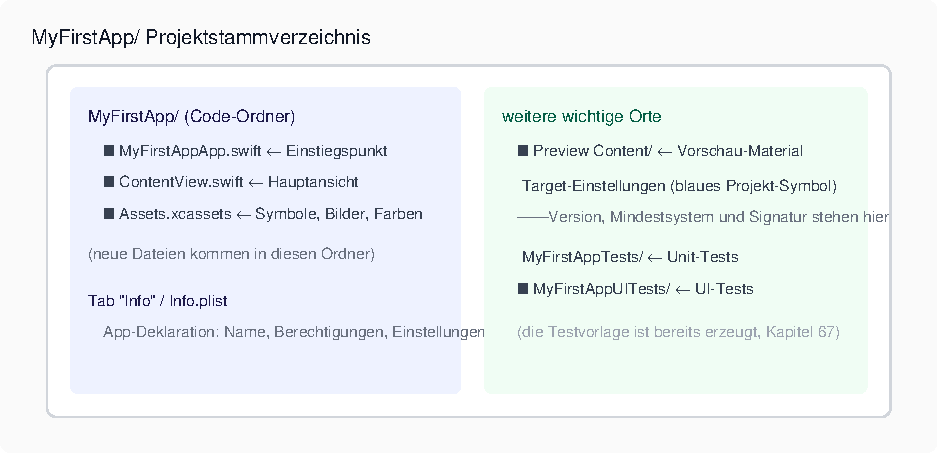
\includegraphics[width=0.92\linewidth]{figures/fig-di-liu-shi-zhang-1}
\\[2pt]\small Abbildung 2: Die Xcode-Projektstruktur, die Einsteiger kennen müssen
\end{center}

\begin{itemize}
  \item MyFirstAppApp.swift: der Programmeinstieg; in SwiftUI sind es nur ein paar Zeilen – „starten, dann die Hauptoberfläche zeigen“;
  \item ContentView.swift: die Hauptansicht; alles, was du gerade siehst, liegt hier;
  \item Assets.xcassets: das Ressourcenlager – Icons, Bilder und Farben liegen hier;
  \item Target-Einstellungen: über das blaue Projektsymbol links hinein; Versionsnummer, minimale iOS-Version und Signatur stehen dort. Auch Anzeigename und Icon der App konfigurierst du hier.
\end{itemize}

\booksection{Debugging auf dem echten Gerät: die App auf dein iPhone bringen}

\booksection{Xcode-Effizienztricks: die fünf „Tastenkürzel-Cheats“ für Einsteiger}

Wenn du diese beherrschst, wirkst du „sehr professionell“:

\begin{center}
\begin{tabularx}{\linewidth}{|X|X|X|}
\hline
\textbf{Aktion} & \textbf{Tastenkürzel} & \textbf{Wirkung} \tabularnewline
\hline
Ausführen & CmdR & Kompilieren und starten \tabularnewline
Canvas-Vorschau öffnen/umschalten & OptionCmd & Der Schalter für WYSIWYG \tabularnewline
Einrückung formatieren & CtrlI & Die Einrückung des ausgewählten Codes automatisch ordnen \tabularnewline
Datei schnell öffnen & CmdO & Dateinamen tippen, sofort offen (am häufigsten gebraucht!) \tabularnewline
Kommentieren/Kommentar aufheben & Cmd/ & Beim Debuggen Code nebenbei ein- und ausschalten \tabularnewline
\hline
\end{tabularx}
\end{center}

\begin{center}\small\color{gray}Die meistgenutzten Xcode-Tastenkürzel (das Einsteiger-Fünfer-Set)\end{center}

Zwei weitere versteckte Boni: mehrere Simulatoren gleichzeitig (iPhone und iPad nebeneinander laufen lassen, um Layouts zu vergleichen) und die Snippet-Bibliothek (häufige Codezeilen ins Snippets-Panel rechts ziehen, beim nächsten Mal per Knopfdruck einfügen) – nutz diese Effizienzwerkzeuge einfach, das Gefühl kommt von selbst.

\booksection{Debugging auf dem echten Gerät: die App auf dein iPhone bringen}

So gut der Simulator auch ist, das echte Gerät ist das Ziel. Auch mit einer kostenlosen Apple ID kannst du auf echten Geräten debuggen:

\begin{enumerate}
  \item iPhone per Datenkabel anschließen (oder kabellos im selben WLAN debuggen);
  \item In der Geräteliste oben in Xcode dein Handy wählen; beim ersten Mal wirst du zum Anmelden mit der Apple ID aufgefordert, die Signatur wird automatisch eingerichtet;
  \item Auf dem iPhone [Einstellungen] [Allgemein] [VPN \& Geräteverwaltung] deinem Entwicklerzertifikat vertrauen;
  \item > drücken, und die App landet auf dem echten Gerät.
\end{enumerate}

\begin{tcbwarn}{Achtung: die „Sieben-Tage-Grenze“ des kostenlosen Kontos}
Eine App mit Signatur einer kostenlosen Apple ID erlischt nach 7 Tagen (ein erneutes Ausführen verlängert die Gültigkeit). Das ist Apples Missbrauchsschutz und reicht für die Lernphase völlig; ein bezahltes Entwicklerkonto (99 US-Dollar pro Jahr) hat diese Grenze nicht, mehr dazu in Kapitel 67.

\end{tcbwarn}

\booksection{Erste Proben + Erste Hilfe bei häufigen Fehlern}

\booksection{Erste Proben + Erste Hilfe bei häufigen Fehlern}

Öffne ContentView.swift, ersetze den Text in Text(“Hello, world!”) durch deinen Namen und drücke CmdR – Sekunden später zeigt der Simulator deinen Namen. Glückwunsch: Du hast die erste vollständige Runde „Code ändern kompilieren installieren ausführen“ absolviert.

\begin{center}
\begin{tabularx}{\linewidth}{|X|X|X|}
\hline
\textbf{Fehlerbild} & \textbf{Häufige Ursache} & \textbf{Gegenmittel} \tabularnewline
\hline
Signing-Fehler & Kein Team gewählt, Zertifikat abgelaufen & In Target Signing dein Konto anhaken; beim kostenlosen Konto einmal neu ausführen \tabularnewline
Simulator bleibt schwarz/öffnet nicht & Beschädigtes Image & Menü Device Erase All Content; oder den Simulator löschen und neu anlegen \tabularnewline
Xcode lädt langsam/installiert nicht & Netzwerkschwankungen beim App Store & Andere Tageszeit wählen; oder das .xip-Offline-Paket von der Apple-Entwicklerseite laden \tabularnewline
\hline
\end{tabularx}
\end{center}

\begin{center}\small\color{gray}Erste-Hilfe-Tabelle für typische Einrichtungsfehler von Einsteigern\end{center}

\begin{tcbpractice}{Jetzt bist du dran: deine „Entwickler-Ritual“-Checkliste abschließen}
(1) Xcode installieren und den Simulator zum Laufen bringen; (2) die eigene App einmal auf dem echten Gerät starten und einen Screenshot als Erinnerung machen; (3) den Hello-Text durch deinen Namen ersetzen; (4) in den Target-Einstellungen den Anzeigenamen auf „Meine erste App“ ändern. Nach diesen vier Schritten bist du jemand mit einem eigenen Werk.

\end{tcbpractice}

\begin{tcbsummary}{Zusammenfassung des Kapitels}
\begin{itemize}
  \item Harte Hürden: Mac + Xcode; ohne Mac zuerst mit Swift Playgrounds auf dem iPad die Sprache lernen
  \item Xcode aus dem App Store installieren; neue Versionen verlangen neue Systeme, Updates nicht aufschieben
  \item Die fünf Elemente beim neuen Projekt: Name, Team, Organisationskennung, SwiftUI, Swift
  \item Projekt-Merksatz: Der Code liegt im Ordner MyFirstApp/; die Target-Einstellungen regeln Version und Signatur
  \item Beim Debuggen auf echten Geräten mit kostenloser Apple ID gilt die 7-Tage-Signaturgrenze; ein bezahltes Konto hat sie nicht
  \item Der Entwickleralltag = Code ändern CmdR Ergebnis ansehen, im ewigen Kreislauf
\end{itemize}

\end{tcbsummary}

\bookchapter{Kapitel 61: Swift im Schnelldurchlauf – die Hauptsprache der Apple-Entwicklung}

\chapterintro{In diesem Kapitel lernen wir die Sprache richtig. Keine Angst – Swift ist berühmt dafür, „einsteigerfreundlich“ zu sein, und du brauchst kein Grammatikbuch auswendig zu lernen: Mit 20 \% der Syntax verstehst und schreibst du 80 \% des Alltagscodes. Den Rest schlägst du nebenbei nach, während du Projekte baust. Merk dir unser Lernprinzip: Verstehen > Auswendiglernen, Anwenden können > Meisterschaft.}

\booksection{Variablen und Typen: den Daten Namen geben}

Ein Programm ist „Daten + Logik“. Eine Variable gibt den Daten einen Namen und speichert sie. Swift deklariert mit let und var:

\begin{lstlisting}[language=Swift]
let name = "Max"        // let: Konstante (standardmäßig empfohlen)
var age = 18             // var: Variable (später änderbar)

age = 19                 // <i class="fas fa-check-circle mr-1"></i> var ist änderbar
// name = "Lena"         // <i class="fas fa-times-circle mr-1"></i> let ist nicht änderbar: Kompilierfehler

let score: Int = 100     // der Typ lässt sich auch explizit angeben
let pi = 3.14            // ohne Angabe wird er automatisch abgeleitet

print("Hallo \(name)")   // String-Interpolation: Backslash + Klammern
\end{lstlisting}

Die gängigen Typen in einer Tabelle:

\begin{center}
\begin{tabularx}{\linewidth}{|X|X|X|}
\hline
\textbf{Typ} & \textbf{Was gespeichert wird} & \textbf{Beispiel} \tabularnewline
\hline
Int & Ganzzahl & 42 \tabularnewline
Double & Dezimalzahl & 3.14 \tabularnewline
String & Text & „Hallo“ \tabularnewline
Bool & wahr/falsch & true / false \tabularnewline
{}[Int] (Array) & Eine Sammlung von Werten & {}[1, 2, 3] \tabularnewline
\hline
\end{tabularx}
\end{center}

\begin{center}\small\color{gray}Swifts gängige Basistypen\end{center}

\begin{tcbinfo}{Tipp: die let-zuerst-Regel}
Das eiserne Gesetz der Swift-Community: standardmäßig let, und var nur, wenn es wirklich nötig ist. Wo let möglich wäre, warnt dich Xcode mit gelbem Text über das var. Diese Gewohnheit erspart dir eine ganze Klasse von Bugs durch „versehentlich geänderte Variablen“ – je weniger sich im Code verändert, desto leichter ist er zu durchdenken.

\end{tcbinfo}

\booksection{Optionals: Swifts „Amulett gegen Abstürze“}

Das ist das wichtigste Konzept in Swift, punktum. In einem Satz: Kann ein Wert unter Umständen „nicht vorhanden“ sein, zwingt dich Swift, diesen Fall zu behandeln – damit ist der „Null-Pointer-Absturz“, dieser branchenweite Albtraum, schon auf Sprachebene ausgemerzt.

\begin{lstlisting}[language=Swift]
var name: String = "Max"   // normaler Typ: darf nie nil sein
// name = nil                // <i class="fas fa-times-circle mr-1"></i> Kompilierfehler: stoppt dich sofort

var nickname: String? = nil  // mit Fragezeichen: nil erlaubt (Optional)
nickname = "Tommy"

// bei Optionals musst du sie "auspacken":
if let n = nickname {        // if let: sicheres Auspacken
    print("Hallo \(n)")
} else {
    print("Noch kein Spitzname")
}

let len = nickname?.count ?? 0   // ?? Standardwert (Nil-Coalescing-Operator)
print(len)
\end{lstlisting}

\begin{tcbwarn}{Achtung: ! ist eine Hochrisiko-Operation}
Im Code nickname! zu schreiben (erzwungenes Entpacken) ist, als riefst du dem Compiler zu: „Ich versichere, dass es nicht nil ist“ – liegst du falsch, stürzt die App auf der Stelle ab. Für Einsteiger gilt: möglichst if let / ?? verwenden, nicht !. Wenn Xcode Code vervollständigt, fügt es gelegentlich eigenmächtig ein ! an – denk daran, das zu entfernen.

\end{tcbwarn}

\booksection{Funktionen und Closures: Logik in „Schaltflächen“ verpacken}

Eine Funktion ist ein Stück Logik mit Namen, wie eine Taste auf der Fernbedienung. Eine Closure dagegen ist eine „Funktion ohne Namen“, die du jederzeit weiterreichen kannst:

\begin{lstlisting}[language=Swift]
// Funktion: Name vorne; Parameter und Rückgabetyp dahinter
func greet(name: String) -> String {
    return "Hallo, \(name)!"
}
print(greet(name: "Max"))     // beim Aufruf mit Parameternamen

// Closure: direkt vor Ort definiert, leicht und direkt
let numbers = [1, 2, 3, 4]
let doubled = numbers.map { $0 * 2 }   // $0 = das aktuelle Element
// [2, 4, 6, 8]

let big = numbers.filter { $0 > 2 }    // filtern
// [3, 4]
\end{lstlisting}

In SwiftUI sind Closures überall: Die geschweiften Klammern hinter Button(“Tippe mich”) \{ ... \} sind genau so eine Closure. Präge dir die Sammlungs-Kombos map, filter und sorted gut ein – künftig sind 90 \% aller Listenverarbeitungen Kombinationen daraus.

\booksection{Structs und Protokolle: Swifts „Lego“-System}

Swifts offizielle Präferenz ist eindeutig: Bevorzugt Structs verwenden; erst wenn Vererbung nötig ist, zu Classes greifen. Structs sind Werttypen – beim Kopieren lebt jedes sein eigenes Leben, was eine ganze Kategorie von Bugs von vornherein ausschließt:

\begin{lstlisting}[language=Swift]
// das Struct: die Daten-Box
struct Record {
    var id = UUID()
    var amount: Double
    var category: String
    var date: Date

    // das Struct bringt seinen "Memberwise Initializer" mit: direkt erstellbar
}
let r = Record(amount: 25.5, category: "Essen", date: Date())

// Protokoll: der Vertrag, "welche Fähigkeiten vorhanden sein müssen"
protocol Identifiable {
    var id: UUID { get }
}
struct Record: Identifiable { ... }   // das Protokoll übernehmen = zusagen, seine Anforderungen zu erfüllen
\end{lstlisting}

In SwiftUI ist fast alles ein struct (View ist lediglich ein Protokoll). Wenn du das jetzt noch nicht ganz verstehst, ist das kein Problem – ab Kapitel 62 begegnet dir das täglich. In der Welt von Swift gilt: Umarme zuerst das struct.

\booksection{Syntax-Spickzettel für absolute Einsteiger}

\begin{center}
\begin{tabularx}{\linewidth}{|X|X|}
\hline
\textbf{Was du tun willst} & \textbf{Schreibweise} \tabularnewline
\hline
Konstante/Variable definieren & \texttt{let x = 1}/\texttt{var x = 1} \tabularnewline
String-Interpolation & "Hallo, \textbackslash{}(name)" \tabularnewline
Funktion definieren & func name(parameter: Typ) -> Rückgabetyp \{ ... \} \tabularnewline
Verzweigung & if Bedingung \{ ... \} else \{ ... \} \tabularnewline
Durchlaufen & for x in array \{ ... \} \tabularnewline
Sicheres Entpacken & if let x = optionalerWert \{ ... \} \tabularnewline
Standardwert & x ?? Standardwert \tabularnewline
Struct definieren & \texttt{struct X \{ var a: Int; var b: String \}} \tabularnewline
Closure & \texttt{\{ \$0 * 2 \}} \tabularnewline
\hline
\end{tabularx}
\end{center}

\begin{center}\small\color{gray}Swift-Syntax-Spickzettel (Einsteigerversion)\end{center}

\begin{tcbpractice}{Jetzt bist du dran: 15 Minuten lang Swift in Playgrounds ausprobieren}
Hast du einen Mac, öffne Xcode Playground; ohne Mac nutze Swift Playgrounds auf dem iPad oder den Web-Playground. Führe jeden Codeabschnitt dieses Kapitels einmal aus, ändere Zahlen und Texte ab und baue absichtlich ein paar Fehler ein, um zu sehen, wie Xcode sie meldet. Diese 15 Minuten nach dem Motto „erst spielen, dann lernen“ machen dir den Einstieg in Kapitel 62 gleich doppelt so leicht.

\end{tcbpractice}

\begin{tcbsummary}{Kapitelfazit}
\begin{itemize}
  \item Erst let, var nur mit Bedacht; Typen werden automatisch abgeleitet, nach dem Doppelpunkt geht auch eine explizite Angabe
  \item Optionals sind Swifts Seele: Kann ein Wert leer sein, musst du ihn behandeln – if let / ?? sind dein Glücksbringer, ! ist eine Hochrisiko-Operation
  \item Funktionsaufrufe tragen Parameternamen; Closure = Funktion ohne Namen, in SwiftUI überall anzutreffen
  \item Bevorzuge structs und halte dich an Protokolle; in SwiftUI ist fast alles ein struct
  \item 20 \% Syntax erledigen 80 \% der Arbeit: erst anwenden, dann meistern
\end{itemize}

\end{tcbsummary}

\bookchapter{Kapitel 62: Oberflächenentwicklung – SwiftUI-Grundlagen}

\chapterintro{Die Oberfläche ist alles, was der Nutzer sieht. SwiftUI ist Apples 2019 vorgestelltes deklaratives UI-Framework – du beschreibst nur, wie die Oberfläche aussieht, und das System kümmert sich automatisch ums Rendern, den Dunkelmodus und alle möglichen Bildschirme. 2026 ist SwiftUI für neue Projekte längst der absolute Standard. In diesem Kapitel lernen wir „Zeichnen“.}

\booksection{SwiftUIs Denkweise: deklarativ statt imperativ}

Die klassische Oberflächenentwicklung ist imperativ: Du kommandierst Schritt für Schritt „Button erstellen an Position (20,30) setzen Farbe festlegen“. SwiftUI ist deklarativ: Du beschreibst direkt „Auf der Oberfläche gibt es einen roten Button mit der Aufschrift ‚Tippe mich'“ – wie gezeichnet und wann neu gezeichnet wird, darum kümmert sich das System selbst.

\begin{lstlisting}[language=Swift]
import SwiftUI

struct ContentView: View {
    var body: some View {      // body: beschreibt, "wie die Oberfläche aussieht"
        VStack {               // vertikal gestapelt
            Text("Hallo, Welt!")
                .font(.largeTitle)      // Modifier: große Überschrift
            Button("Klick mich") {
                print("Geklickt!")
            }
            .buttonStyle(.borderedProminent)  // ausgefüllter blauer Button
        }
        .padding()
    }
}
\end{lstlisting}

Der Kern: Ein View ist ein struct, das das View-Protokoll erfüllt, die body-Eigenschaft beschreibt die Oberfläche, und mit .modifier()-Ketten verpasst du ihr den „Feinschliff“. Das ist bereits das gesamte Fundament von SwiftUI.

\booksection{Grundlegende Views: Text, Button, Textfeld, Bild}

\begin{center}
\begin{tabularx}{\linewidth}{|X|X|X|}
\hline
\textbf{View} & \textbf{Funktion} & \textbf{Beispiel} \tabularnewline
\hline
Text & Text anzeigen & Text("Hallo") \tabularnewline
Button & Button & Button("Tippe mich") \{ Aktion \} \tabularnewline
TextField & Textfeld & TextField("Hinweis", text: \$eingabe) \tabularnewline
Image & Bild anzeigen & \texttt{Image(systemName: "star.\allowbreak fill")} \tabularnewline
\hline
\end{tabularx}
\end{center}

\begin{center}\small\color{gray}Die vier Grundviews von SwiftUI\end{center}

Beachte Image(systemName:) – Apple liefert die SF-Symbols-Symbolbibliothek mit (mehrere tausend kostenlose Icons). Ein Name wie “star.fill” genügt, und schon erscheint ein ausgefüllter Stern. Das ist ein versteckter Bonus der iOS-Entwicklung: Beim Bau von Oberflächen musst du kaum noch nach Icon-Material suchen.

\booksection{Das Layout-Trio: VStack, HStack und ZStack}

\begin{itemize}
  \item VStack: untereinander (wie in der Essensschlange);
  \item HStack: nebeneinander (wie nebeneinander auf der Sitzbank);
  \item ZStack: übereinander gestapelt (wie ein Haufen Spielkarten – ideal für Badges und Overlays).
\end{itemize}

\begin{lstlisting}[language=Swift]
VStack(alignment: .leading, spacing: 12) {
    HStack {
        Text("Rechnung")
        Spacer()                 // elastischer Abstand: schiebt das Rechte ans Ende
        Text("-25.5 Yuan").foregroundColor(.red)
    }
    Divider()                    // Trennlinie
    Text("Notiz: Mittagessen")
}
.padding(16)                     // Abstand an allen Seiten
.background(Color(.systemGray6)) // heller grauer Hintergrund
.cornerRadius(12)                // abgerundete Ecken

// die Reihenfolge der Modifier zählt: erst padding, dann background; der Hintergrund ohne Rand
\end{lstlisting}

\begin{tcbwarn}{Achtung: Die Reihenfolge der Modifier ist entscheidend}
padding(16).background(grau) und background(grau).padding(16) wirken unterschiedlich – Ersteres heißt „erst Abstand, dann Farbe“ (der Hintergrund umfasst den Abstand nicht), Letzteres „erst Farbe, dann Abstand“ (der Hintergrund umfasst den Abstand). Genau daher stammen die seltsamen weißen Ränder, die Einsteiger am häufigsten verwirren. Im Zweifel tausch die Reihenfolge – die Vorschau verrät dir sofort die Antwort.

\end{tcbwarn}

\booksection{State und Binding: die Oberfläche zum „Leben“ erwecken}

Eine statische Oberfläche ist langweilig. SwiftUIs Regel: Die Oberfläche spiegelt jederzeit treu den Zustand wider – ändert sich der Zustand, zeichnet sie sich automatisch neu.

\begin{lstlisting}[language=Swift]
struct CounterView: View {
    @State private var count = 0   // @State: ändert sich dieser Wert, muss neu gezeichnet werden

    var body: some View {
        VStack {
            Text("Du hast \(count) Mal geklickt")
            Button("Klick +1") {
                count += 1          // Zustand ändern, die Oberfläche aktualisiert sich automatisch
            }
        }
    }
}
\end{lstlisting}

Textfelder brauchen eine „bidirektionale Bindung“ – das \$-Zeichen übergibt Wert und Änderungsrecht zusammen:

\begin{lstlisting}[language=Swift]
struct InputView: View {
    @State private var text = ""

    var body: some View {
        TextField("Etwas eingeben", text: $text)  // Zweiwege-Bindung mit $
            .textFieldStyle(.roundedBorder)
        Text("Du hast eingegeben: \(text)")   // aktualisiert sich live während der Eingabe
    }
}
\end{lstlisting}

Nutzeraktion

Zustand ändert sich (count += 1)

SwiftUI bemerkt die Änderung

Zeichnet neu (body wird neu berechnet)

\begin{center}\small\color{gray}Abbildung 3: SwiftUIs unidirektionaler Datenfluss von „Zustand Oberfläche“\end{center}

\booksection{Vorschau, Themes und Animationen: SwiftUIs „Geheimwaffen“}

\begin{itemize}
  \item Das \#Preview-Makro: Ergänze am Dateiende \#Preview \{ ContentView() \}, und die Leinwand rechts rendert in Echtzeit – Code ändern, sofort sehen;
  \item Dunkelmodus gratis: Systemfarben verwenden (Color(.systemGray6), .primary) statt fest codierter Farben – dann passt sich der Dunkelmodus automatisch an, ohne eine einzige Zusatzzeile;
  \item Animation mit einer Zeile: withAnimation \{ count += 1 \} oder .animation(.default, value: count) am View – Übergänge werden seidenweich.
\end{itemize}

\begin{lstlisting}[language=Swift]
struct AnimatedHeartView: View {
    @State private var liked = false

    var body: some View {
        Button {
            withAnimation(.spring(duration: 0.4)) {
                liked.toggle()
            }
        } label: {
            Image(systemName: liked ? "heart.fill" : "heart")
                .font(.system(size: 48))
                .foregroundColor(liked ? .red : .gray)
                .scaleEffect(liked ? 1.3 : 1.0)
        }
    }
}
\end{lstlisting}

\begin{tcbinfo}{Tipp: erst die Funktion, dann die Animation}
Der typische Anfängerfehler: über Animationen grübeln, obwohl die Oberfläche noch gar nicht stimmt. Bring erst die Funktion zum Laufen und lege die Effekte am Ende gebündelt auf – Animationen sind das i-Tüpfelchen, Funktionen sind die Rettung in der Not. Auch das folgt unserem Prinzip „Einfachheit zuerst“.

\end{tcbinfo}

\begin{tcbpractice}{Jetzt bist du dran: Baue einen „Stimmungs-Button“}
\booksection{Modifier-Spickzettel: eine Seite in der Hand, und die Oberfläche sitzt}

\begin{center}
\begin{tabularx}{\linewidth}{|X|X|}
\hline
\textbf{Was du erreichen willst} & \textbf{Modifier} \tabularnewline
\hline
Abstand & \texttt{.\allowbreak padding(16)} \tabularnewline
Eckenradius & \texttt{.\allowbreak cornerRadius(12)} \tabularnewline
Hintergrundfarbe & \texttt{.\allowbreak background(Color(.\allowbreak systemGray6))} \tabularnewline
Schrift und Schriftgröße & \texttt{.\allowbreak font(.\allowbreak title.\allowbreak bold())}/\texttt{.\allowbreak font(.\allowbreak system(size: 20))} \tabularnewline
Vordergrundfarbe (Text/Icons) & \texttt{.\allowbreak foregroundColor(.\allowbreak red)} \tabularnewline
Volle Breite füllen & \texttt{.\allowbreak frame(maxWidth: .\allowbreak infinity)} \tabularnewline
Feste Größe & \texttt{.\allowbreak frame(width: 100, height: 44)} \tabularnewline
Ausrichtung & \texttt{VStack(alignment: .\allowbreak leading)} \tabularnewline
Transparenz & \texttt{.\allowbreak opacity(0.\allowbreak 6)} \tabularnewline
Schatten & \texttt{.\allowbreak shadow(radius: 5)} \tabularnewline
Tipp-Geste & \texttt{.\allowbreak onTapGesture \{ .\allowbreak .\allowbreak .\allowbreak  \}} \tabularnewline
Tastaturtyp & \texttt{.\allowbreak keyboardType(.\allowbreak decimalPad)} \tabularnewline
\hline
\end{tabularx}
\end{center}

\begin{center}\small\color{gray}SwiftUI-Modifier-Spickzettel\end{center}

Kein Problem, wenn du dir nichts merkst – diese Seite ist zum Nachschlagen da. Am häufigsten brauchst du ohnehin nur die ersten vier: padding, Eckenradius, Hintergrund, Schrift.

Verwandle das Vorlagenprojekt in einen Stimmungsschalter: ein Button, der beim Tippen im Kreis zwischen fröhlich traurig wütend wechselt, während Text und Hintergrundfarbe mitwechseln. Tipp: Speichere die drei Paare (Text + Farbe) in einem Array, den Index in @State und tippe dich mit (index + 1) \% 3 weiter. Schick das Ergebnis hinterher an deine Freunde – und ernte die erste Welle von „Wow, du kannst Apps bauen!“.

\end{tcbpractice}

\begin{tcbsummary}{Kapitelfazit}
\begin{itemize}
  \item SwiftUI ist deklarativ: Du beschreibst, wie etwas aussieht, das System zeichnet und zeichnet neu
  \item View = struct, das das View-Protokoll erfüllt; body beschreibt die Oberfläche; Modifier verpassen ihr den „Feinschliff“
  \item Die vier Grundviews: Text / Button / TextField / Image; die SF-Symbols-Bibliothek liefert gratis Icons ohne Ende
  \item Das Layout-Trio: VStack untereinander, HStack nebeneinander, ZStack übereinander; Spacer ist der flexible Zwischenraum
  \item @State erweckt die Oberfläche zum Leben; \$ liefert die bidirektionale Bindung ans Textfeld
  \item \#Preview zeigt sofort, was du tust; Systemfarben passen sich automatisch an den Dunkelmodus an; withAnimation setzt Effekte mit einer Zeile
\end{itemize}

\end{tcbsummary}

\bookchapter{Kapitel 63: Views, State und Navigation}

\chapterintro{Einseitige Spielereien kannst du bereits. Dieses Kapitel löst die zwei Fragen des „Erwachsenwerdens“: wie du zwischen mehreren Seiten hin- und herspringst (Navigation) und wie Daten zwischen den Seiten fließen (State-Management). Nach diesem Kapitel baust du das klassische Mehrseiten-Gerüst „Liste Detail Bearbeiten“.}

\booksection{Das Datenfluss-Panorama des State-Managements}

SwiftUI hat mehr als nur @State als State-Werkzeug. Sieh dir zuerst diese Übersicht an, um zu verstehen, „wann du welches einsetzt“:

\begin{center}
\begin{tabularx}{\linewidth}{|X|X|X|X|}
\hline
\textbf{Werkzeug} & \textbf{Zuständig für} & \textbf{Wer es nutzt} & \textbf{Typischer Einsatzfall} \tabularnewline
\hline
@State & Seiteneigener, temporärer Zustand & Das aktuelle View & Zähler, Textfeldeingaben \tabularnewline
@Binding & Zustand von jemand anderem ausleihen & Kind-View ändert Eltern-View & Eigene Komponenten \tabularnewline
@StateObject / @Observable & Seitenübergreifend geteilte Logik & ViewModel & Datenladen, Geschäftslogik \tabularnewline
@EnvironmentObject / .environment & Global geteilter Zustand & Die ganze App & Anmeldestatus, Theme-Einstellungen \tabularnewline
\hline
\end{tabularx}
\end{center}

\begin{center}\small\color{gray}Überblick über SwiftUIs State-Werkzeuge (2026: @Observable ist längst Standard)\end{center}

\begin{lstlisting}[language=Swift]
// der moderne Weg ab iOS 17+: das @Observable-Makro (für neue Projekte empfohlen)
import Observation

@Observable
class CounterModel {                 // das View Model
    var count = 0
    func increment() { count += 1 }
}

struct CounterView: View {
    @State private var model = CounterModel()   // hält das Modell

    var body: some View {
        VStack {
            Text("Du hast \(model.count) Mal geklickt")
            Button("Klick mich") { model.increment() }
        }
    }
}
\end{lstlisting}

Knallharter Rat für Einsteiger: Seiteneigen @State; seitenübergreifend oder mit Logik @Observable-Klasse. @StateObject/@ObservableObject aus älteren Tutorials ist die Schreibweise der Vorgängergeneration – lesen können genügt, für neuen Code gilt das oben Gesagte.

\booksection{NavigationStack: der „Stapel“ für Seitenwechsel}

Ab iOS 16 übernimmt NavigationStack die Mehrseiten-Navigation – wie ein Stapel Teller: einer kommt oben drauf, und beim Zurückgehen wird jeder einzeln wieder abgenommen:

\begin{lstlisting}[language=Swift]
struct HomeView: View {
    var body: some View {
        NavigationStack {
            List {
                NavigationLink("Max' Ausgabenbuch") {
                    DetailView(name: "Max' Ausgabenbuch")   // Zielseite
                }
                NavigationLink("Lenas Ausgabenbuch") {
                    DetailView(name: "Lenas Ausgabenbuch")
                }
            }
            .navigationTitle("Liste der Ausgabenbücher")   // große Überschrift oben
        }
    }
}

struct DetailView: View {
    let name: String
    var body: some View {
        Text("Details zu \(name)")
            .navigationTitle(name)
            .navigationBarTitleDisplayMode(.inline)
    }
}
\end{lstlisting}

NavigationLink ist schlicht ein „antippbarer Sprunglink“; navigationTitle erzeugt automatisch Navigationstitel und Zurück-Button. Für programmatisches Navigieren (etwa nach „Speichern“ automatisch zurück) schließt du die aktuelle Seite mit @Environment(\textbackslash{}.dismiss) – mit dieser Kombination hast du 90 \% aller Navigationsbedürfnisse abgedeckt.

\booksection{Dialoge und untere Reiter: sheet und TabView}

Neben dem „Seitenschieben“ gibt es zwei klassische Interaktionsformen:

\begin{lstlisting}[language=Swift]
// 1. Sheet von unten, halber oder ganzer Bildschirm (der Liebling von Eingabeformularen)
struct HomeView: View {
    @State private var showAdd = false
    var body: some View {
        Button("Ausgabe erfassen") { showAdd = true }
            .sheet(isPresented: $showAdd) {
                AddRecordView()     // die sich öffnende Erfassungsansicht
            }
    }
}

// 2. untere Tab-Leiste (das "Skelett" der App)
struct MainTabView: View {
    var body: some View {
        TabView {
            RecordListView()
                .tabItem { Label("Buch", systemImage: "book") }
            StatsView()
                .tabItem { Label("Statistik", systemImage: "chart.pie") }
            SettingsView()
                .tabItem { Label("Einstellungen", systemImage: "gear") }
        }
    }
}
\end{lstlisting}

\begin{tcbinfo}{Tipp: Wann nimmt man was?}
Faustregel: Für den Hauptablauf Seiten mit NavigationStack schieben (Liste Detail), für kurzzeitige Aktionen den sheet-Dialog (Anlegen, Bearbeiten, Bestätigen) und für gleichrangige Hauptbereiche TabView (untere Reiter). Die Kombination aus allen dreien ist das Gerüst der allermeisten Apps.

\end{tcbinfo}

\booksection{List: iOS' Alleskönner-Liste}

Der meistgenutzte und am typischsten „apple-artige“ Baustein unter iOS ist List – mit Trennlinien, Wisch-löschen und Tipp-Highlight ab Werk:

\begin{lstlisting}[language=Swift]
struct RecordListView: View {
    @State private var records = ["Mittagessen 25.5", "U-Bahn 6.0", "Gehalt +8000"]

    var body: some View {
        List {
            ForEach(records, id: \.self) { r in
                Text(r)
            }
            .onDelete { indexSet in          // nach links wischen zum Löschen
                records.remove(atOffsets: indexSet)
            }
        }
    }
}
\end{lstlisting}

Liste + NavigationLink + sheet + TabView – kombiniere diese vier Bausteine, und du kannst bereits das komplette App-Gerüst „Buchungsliste Detail öffnen auf + tippen, Eingabe-Dialog erscheint“ bauen. Genau so entsteht das Haushaltsbuch-Projekt im nächsten Kapitel.

\begin{tcbpractice}{Jetzt bist du dran: Baue ein „Drei-Seiten-Gerüst“}
\booksection{Der App-Lebenszyklus: Vordergrund und Hintergrund}

Ähnlich wie der Activity-Lebenszyklus bei Android durchläuft auch eine iOS-App Zustandswechsel von „Geburt, Vordergrund, Hintergrund, Tod“. In SwiftUI beobachtest du das über den Environment-Wert scenePhase:

\begin{lstlisting}[language=Swift]
@main
struct MyApp: App {
    @Environment(\.scenePhase) private var phase

    var body: some Scene {
        WindowGroup {
            ContentView()
        }
        .onChange(of: phase) { _, newPhase in
            switch newPhase {
            case .active:    print("wieder vorn: Aktualisierung fortsetzen")
            case .inactive:  print("im Übergang (Anruf oder Moment des Wechsels nach hinten)")
            case .background: print("in den Hintergrund: Entwurf sichern")
            @unknown default: break
            }
        }
    }
}
\end{lstlisting}

Typische Einsätze: Daten auffrischen, wenn die App wieder in den Vordergrund kommt; Entwürfe speichern, wenn sie in den Hintergrund geht. iOS geht mit Hintergrundbetrieb streng ins Gericht – normale Apps werden bald nach dem Wechsel in den Hintergrund angehalten (eingefroren). Rechne nicht damit, heimlich Schwerstarbeit im Hintergrund zu leisten; für zeitgesteuerte Aufgaben nutze die lokalen Benachrichtigungen aus Kapitel 68, keinen „Dauerbetrieb im Hintergrund“.

Baue eine Fake-Daten-Version des Haushaltsbuch-Gerüsts: TabView mit drei Reitern (Buchungen/Statistik/Einstellungen) die Buchungsseite zeigt Fake-Daten in einer List, ein Tipp auf eine Zeile springt zum Detail (NavigationStack) der “+”-Button oben rechts öffnet den Eingabe-Dialog als sheet. Kein Speichern, kein Netz – reine Gerüstübung. Steht dieses Gerüst, ist es in Kapitel 65 nur noch ein Katzensprung, echte Daten einzufüllen.

\end{tcbpractice}

\begin{tcbsummary}{Kapitelfazit}
\begin{itemize}
  \item Die vier State-Werkzeuge: @State (seiteneigen), @Binding (ausgeliehen), @Observable (Logik), .environment (global)
  \item In neuen Projekten schreibst du ViewModels mit dem @Observable-Makro; @ObservableObject aus alten Tutorials: lesen können genügt
  \item NavigationStack schiebt Seiten; @Environment(\textbackslash{}.dismiss) ermöglicht programmatisches Zurück
  \item Hauptablauf: Seiten schieben; kurzzeitige Aktionen: sheet; gleichrangige Hauptbereiche: TabView
  \item List ist die Alltagsliste: Trennlinien und Wisch-löschen ab Werk
\end{itemize}

\end{tcbsummary}

\bookchapter{Kapitel 64: Datenspeicherung und Netzwerkanfragen}

\chapterintro{Eine App, die nur „angeschaut“ werden kann, ist tot; erst eine App, die Daten speichern und sich mit dem Netz verbinden kann, lebt. In diesem Kapitel lernst du das „Trio“ der iOS-Datenschicht kennen: UserDefaults (kleine Einstellungen speichern), SwiftData (strukturierte Daten speichern), URLSession (mit dem Server sprechen), dazu Codable fürs JSON-Parsen und das moderne async/await. Danach schreibst du echte Apps, die sich Gewohnheiten ihrer Nutzer merken und ihre Inhalte aktuell halten.}

\booksection{Welche Speicherlösung passt? Erst ein Blick auf diese Tabelle}

\begin{center}
\begin{tabularx}{\linewidth}{|X|X|X|X|}
\hline
\textbf{Lösung} & \textbf{Wofür geeignet} & \textbf{Eigenschaften} & \textbf{Wo in diesem Buch verwendet} \tabularnewline
\hline
UserDefaults & Verstreute Kleinkonfiguration (Schalter, Präferenzen) & Schlüssel-Wert-Paare, simpel und direkt & Einstellungen in Kapitel 65, Lieblingsstädte in Kapitel 66 \tabularnewline
SwiftData & Strukturierte Daten (Buchungen, Einträge) & Offizieller Datenbank-Wrapper, Deklaration mit einer @Model-Zeile & Buchungseinträge in Kapitel 65 \tabularnewline
URLSession & (nicht speichern, aus dem Netz holen) Serverdaten & Netzwerkframework ab Werk, keine Drittanbieter-Abhängigkeiten & Wetterdaten in Kapitel 66 \tabularnewline
\hline
\end{tabularx}
\end{center}

\begin{center}\small\color{gray}Die Arbeitsteilung des Daten-Trios\end{center}

Merke dir den Spruch: „Kleine Einstellungen in UserDefaults, Datenmengen in SwiftData, Daten von außen über URLSession“. Core Data aus älteren Tutorials funktioniert weiterhin (SwiftData ist im Grunde sein modernes Gewand), und handgeschriebenes SQLite fasst du praktisch nie an – lerne gleich das Neue und geh nicht den alten Weg.

\booksection{UserDefaults: kleine Einstellungen ablegen}

\begin{lstlisting}[language=Swift]
// schreiben: Wert speichern
UserDefaults.standard.set(true, forKey: "isDarkMode")
UserDefaults.standard.set("Berlin", forKey: "favoriteCity")

// lesen: herausholen (gibt es nichts, kommt der Standardwert)
let isDark = UserDefaults.standard.bool(forKey: "isDarkMode")
let city = UserDefaults.standard.string(forKey: "favoriteCity") ?? "Berlin"

// löschen: einen Schlüssel entfernen
UserDefaults.standard.removeObject(forKey: "isDarkMode")
\end{lstlisting}

Beachte: Es taugt nur für verstreute Mini-Einstellungen – bei Dutzenden bis Hunderten von Einträgen gib die Sache an SwiftData weiter. Missbrauche UserDefaults nicht als Datenbank (das bremst den App-Start und macht Abfragen umständlich).

\booksection{SwiftData: den Daten ein „richtiges Zuhause“ geben}

SwiftData ist Apples offizielle Datenbanklösung ab iOS 17 und vereinfacht „Tabelle anlegen, hinzufügen, löschen, ändern, abfragen“ aufs Äußerste – eine einzige @Model-Anmerkung, und aus der Datenklasse wird eine Datenbanktabelle:

\begin{lstlisting}[language=Swift]
import SwiftData

// 1. @Model: diese Klasse wird automatisch zur "Tabelle"
@Model
class Record {
    var amount: Double
    var category: String
    var note: String
    var date: Date

    init(amount: Double, category: String, note: String, date: Date) {
        self.amount = amount
        self.category = category
        self.note = note
        self.date = date
    }
}

// 2. den Container am App-Einstiegspunkt anhängen
@main
struct MyApp: App {
    var body: some Scene {
        WindowGroup {
            ContentView()
        }
        .modelContainer(for: Record.self)   // Datenbank bereit
    }
}

// 3. in der View liest man mit @Query und schreibt mit @Environment
struct RecordListView: View {
    @Query(sort: \Record.date, order: .reverse) var records: [Record]
    @Environment(\.modelContext) private var context

    var body: some View {
        List(records) { r in
            Text("\(r.category) \(r.amount) Yuan")
        }
    }

    func add(amount: Double, category: String) {
        let r = Record(amount: amount, category: category, note: "", date: Date())
        context.insert(r)     // speichern
        try? context.save()   // auf Disk schreiben
    }
}
\end{lstlisting}

Diese Vorlage aus „@Model + modelContainer + @Query“ kannst du wortwörtlich in jedes deiner Projekte übernehmen – einfach die Feldnamen austauschen. Ändern sich die Daten, aktualisiert @Query die Oberfläche automatisch – einfach wunderbar.

\booksection{Codable: JSON „übersetzen“}

Serverdaten liegen meist als JSON-Text vor. Swifts Codable-Protokoll lässt die Umwandlung „JSON Struct“ automatisch geschehen – passen die Feldnamen, tritt der Zauber in Kraft:

\begin{lstlisting}[language=Swift]
// JSON: {"name":"Berlin","main":{"temp":26.5},"weather":[{"description":"Klar"}]}
struct WeatherResponse: Codable {
    let name: String
    let main: Main
    let weather: [Weather]
}
struct Main: Codable { let temp: Double }
struct Weather: Codable { let description: String }

// von JSON-String zu Struct
let decoder = JSONDecoder()
let data = jsonString.data(using: .utf8)!
let result = try decoder.decode(WeatherResponse.self, from: data)
print(result.weather[0].description)   // "Klar"
\end{lstlisting}

Eisernes Gesetz: Erst das real zurückkommende JSON ansehen, dann die Felder definieren. Viele „Parsing fehlgeschlagen“-Bugs beruhen auf vertippten Feldnamen oder falsch geratenen Typen (der Server schickt den String “26.5”, du deklarierst Double) – gib das Roh-JSON per print aus und gleiche es ab, dann sitzt die Ursache in zehn Sekunden.

\booksection{URLSession + async/await: mit dem Server sprechen}

Für Netzwerkzugriffe nutzt iOS das ab Werk mitgelieferte URLSession, kombiniert mit Swifts async/await (asynchronen Funktionen) – „aufs Netz warten“ wird so selbstverständlich wie „aufs Paket warten“:

\begin{lstlisting}[language=Swift]
struct WeatherService {
    // asynchrone Funktion: async markiert "ich muss kurz warten", throws markiert "kann fehlschlagen"
    func fetchWeather(city: String) async throws -> WeatherResponse {
        let url = URL(string:
            "https://api.example.com/weather?city=\(city)")!
        let (data, _) = try await URLSession.shared.data(from: url)
        return try JSONDecoder().decode(WeatherResponse.self, from: data)
    }
}

// Aufrufstelle (in .task):
.task {
    do {
        let weather = try await service.fetchWeather(city: "Berlin")
        // Oberfläche aktualisieren …
    } catch {
        print("Fehler: \(error)")
    }
}
\end{lstlisting}

\textbf{Stolperfalle: zwei eiserne Netzwerkgesetze}\par

1) Netzwerkzugriffe immer mit async/await, den Haupt-Thread niemals blockieren – eine eingefrorene Oberfläche ist eine katastrophale Erfahrung. Swifts strukturierte Nebenläufigkeit macht das sehr natürlich, aber vergiss try await und do/catch nicht. 2) ATS verbietet standardmäßig Klartext-HTTP: iOS verlangt HTTPS. Beim Testen eines lokalen http://-Dienstes musst du in Info.plist vorübergehend eine Ausnahme öffnen (NSAppTransportSecurity), doch ein echtes Produkt muss komplett über HTTPS laufen – auch das Review schaut genau darauf.

\begin{tcbpractice}{Jetzt bist du dran: eine kleine „Zitat-des-Tages“-App}
\booksection{Auch Netzwerkfehler „staffeln“: nicht jeden Fehler wahllos an den Nutzer werfen}

Keine Verbindung, Zeitüberschreitung, 404, Serverfehler 500 … Bei verschiedenen Fehlern sollte der Nutzer verschiedene Worte zu sehen bekommen:

\begin{lstlisting}[language=Swift]
func friendlyMessage(_ error: Error) -> String {
    if let urlError = error as? URLError {
        switch urlError.code {
        case .notConnectedToInternet: return "Kein Netz, Verbindung prüfen?"
        case .timedOut:               return "Zeitüberschreitung, später nochmal versuchen?"
        case .cannotFindHost:         return "Server nicht gefunden"
        default:                      return "Netzwerkproblem: \(urlError.code)"
        }
    }
    if let d = error as? DecodingError {
        return "Falsches Datenformat (die API hat sich vielleicht geändert)"
    }
    return "Fehler: \(error.localizedDescription)"
}
\end{lstlisting}

Dem Nutzer „verständliche Worte“ zeigen, dem Log die „Originalworte“ (das komplette error per print ausgeben). Wirf dem Nutzer den englischen Fachchinesisch-Text von error.localizedDescription nicht direkt hin – Produktqualität steckt genau in solchen Details.

Such dir eine kostenlose Zitate-API (etwa hitokoto und Ähnliches), hole mit URLSession + async/await das „Zitat des Tages“, zeige es mitten auf dem Bildschirm und ergänze einen Button „Nächstes Zitat“. Speichere Lieblingssätze zusätzlich mit SwiftData in einer „Favoriten“-Sammlung. Diese Übung nutzt UserDefaults/SwiftData/Codable/URLSession allesamt einmal durch – hast du sie fertig, sind Kapitel 7 und 8 ein Kinderspiel.

\end{tcbpractice}

\begin{tcbsummary}{Kapitelfazit}
\begin{itemize}
  \item Merkspruch: Kleine Einstellungen in UserDefaults, Datenmengen in SwiftData, Daten von außen über URLSession
  \item SwiftDatas drei Kernzüge: die Tabelle mit @Model deklarieren, den Container mit modelContainer anhängen, mit @Query lesen und mit context.insert schreiben
  \item Codable „übersetzt“ JSON automatisch: Passen die Felder, tritt der Zauber in Kraft
  \item URLSession + async/await: aufs Netz warten wie aufs Paket; do/catch fängt Fehler ab
  \item Zwei eiserne Gesetze: Haupt-Thread nicht blockieren; echte Produkte müssen HTTPS nutzen (ATS)
\end{itemize}

\end{tcbsummary}

\bookchapter{Kapitel 65: Projekt 1 – Mein Haushaltsbuch (Lokalversion)}

\chapterintro{Willkommen bei deinem ersten „richtigen Projekt“. Dieses Haushaltsbuch kommt zwar ohne Netz aus, ist aber komplett ausgestattet: Buchungen erfassen, Verlauf ansehen, monatliche Auswertung, Löschen und Ändern. Wenn du fertig bist, hast du den kompletten Ablauf „Daten Logik Oberfläche“ einmal durchlaufen. Wilde nicht gleich den Code ab – erst durchdenken, dann anpacken; das ist unser bewährtes Prinzip.}

\booksection{Anforderungen überdenken: erst fünf Fragen stellen}

\begin{center}
\begin{tabularx}{\linewidth}{|X|X|}
\hline
\textbf{Element} & \textbf{Antwort} \tabularnewline
\hline
Who (für wen?) & Für dich selbst; Familie und Freunde gehen auch \tabularnewline
What (was?) & Einnahmen/Ausgaben erfassen, Verlauf ansehen, Monatsbilanz, Auswertung nach Kategorien \tabularnewline
Why (warum?) & Übung + herausfinden, wohin das Geld geht \tabularnewline
How (wie?) & Swift + SwiftUI + SwiftData + MVVM, rein lokal ohne Backend \tabularnewline
Constraint (Randbedingungen) & In einer Woche fertig; mindestens iOS 17 (SwiftData-Voraussetzung) \tabularnewline
\hline
\end{tabularx}
\end{center}

\begin{center}\small\color{gray}Die fünf Anforderungselemente des Haushaltsbuchs\end{center}

Dann zerlegst du das Ganze in kleine Schritte, nach denen jeweils etwas Benutzbares entsteht: 1) die SwiftData-Datenschicht bauen (eine Buchung speichern können); 2) die Listenseite (Verlauf ansehen); 3) den Eingabe-Dialog (Buchung hinzufügen); 4) Löschen und Bearbeiten; 5) die Monatsbilanz-Karte. Nach jedem erledigten Schritt ist die App ein „brauchbares Ding“.

\booksection{Die Datenschicht: den „Buchungen“ ein Zuhause geben}

Definiere zuerst, wie eine Buchung aussieht – die Felder sollen ausreichen, aber nicht gierig sein:

\begin{lstlisting}[language=Swift]
import SwiftData

@Model
class Record {
    var type: String      // "income" Einnahme | "expense" Ausgabe
    var amount: Double    // Betrag (Yuan)
    var category: String  // Kategorie: Essen, Verkehr, Gehalt …
    var note: String      // Notiz (optional)
    var date: Date        // Buchungsdatum

    init(type: String, amount: Double, category: String, note: String = "", date: Date = Date()) {
        self.type = type
        self.amount = amount
        self.category = category
        self.note = note
        self.date = date
    }
}
\end{lstlisting}

\begin{tcbinfo}{Tipp: Warum Double für den Betrag?}
Seröse Finanz-Apps verwenden Decimal (exakte Dezimalzahlen), um Rundungsfehler bei Gleitkommazahlen zu vermeiden (das alte Problem, dass 0,1 + 0,2 $\neq$ 0,3). Für ein Übungsprojekt reicht Double völlig; baust du eines Tages ein echtes Finanzprodukt, denk an den Wechsel zu Decimal oder ein „Int in Cent“ – eine Falle, in die unzählige Vorgänger getappt sind.

\end{tcbinfo}

\booksection{MVVM: Oberfläche und Logik „ziehen getrennte Wege“}

Die Oberfläche direkt auf die Datenbank zugreifen lassen? Läuft zwar, aber der Oberflächencode wird lang und unappetitlich. Die MVVM-Architektur sorgt für klare Zuständigkeit: View (Oberfläche) zeichnet nur, ViewModel (Logikzentrale) kümmert sich um die Daten, Model (SwiftData) um die Speicherung.

View (SwiftUI-Oberfläche)

ViewModel (@Observable als Logik-Zentrale)

Model (Datenlayer mit SwiftData)

\begin{center}\small\color{gray}Abbildung 4: Die drei Ebenen von MVVM – Daten fließen nur in eine Richtung, und keine Ebene greift einer anderen ins Handwerk\end{center}

\begin{lstlisting}[language=Swift]
import Observation

@Observable
class RecordViewModel {
    var records: [Record] = []
    private let context: ModelContext

    init(context: ModelContext) { self.context = context }

    func load() {
        // Filtern mit #Predicate von SwiftData + Sortierung
        let descriptor = FetchDescriptor<Record>(
            sortBy: [SortDescriptor(\.date, order: .reverse)]
        )
        records = (try? context.fetch(descriptor)) ?? []
    }

    func add(type: String, amount: Double, category: String, note: String) {
        let r = Record(type: type, amount: amount, category: category, note: note)
        context.insert(r)
        try? context.save()
        load()                       // neu laden; die Oberfläche aktualisiert sich
    }

    func delete(_ record: Record) {
        context.delete(record)
        try? context.save()
        load()
    }
}
\end{lstlisting}

In der Oberfläche @State private var vm = RecordViewModel(...) anlegen und die Liste direkt aus vm.records rendern – ändern sich die Daten, aktualisiert sich die Oberfläche automatisch.

\booksection{Die Oberfläche: Listenseite + Eingabe-Dialog}

\begin{lstlisting}[language=Swift]
struct RecordListView: View {
    @State private var vm: RecordViewModel
    @State private var showAdd = false

    var body: some View {
        NavigationStack {
            List {
                Section("Saldo des Monats") {          // Zusammenfassungs-Karte
                    SummaryRow(records: vm.records)
                }
                Section("Umsätze") {
                    ForEach(vm.records) { r in
                        RecordRow(record: r)
                    }
                    .onDelete { idx in
                        idx.forEach { vm.delete(vm.records[$0]) }
                    }
                }
            }
            .navigationTitle("Mein Ausgabenbuch")
            .toolbar {
                Button { showAdd = true } label: {
                    Image(systemName: "plus")
                }
            }
            .sheet(isPresented: $showAdd) {
                AddRecordView(vm: vm)          // Eingabedialog
            }
        }
    }
}
\end{lstlisting}

Wichtige Punkte für den Eingabe-Dialog: für das Betragsfeld .keyboardType(.decimalPad) (Zifferntastatur) verwenden, für Einnahmen/Ausgaben ein segmentiertes Steuerelement (Picker), die Kategorie über ein Menü wählen, und bei „Speichern“ vm.add(...) aufrufen und den Dialog mit dismiss() schließen.

\begin{tcbwarn}{Achtung: Bei der Eingabeprüfung nicht faulenzen}
Das Betragsfeld musst du unbedingt prüfen: Leere Werte, negative Zahlen und unzulässige Eingaben wie “abc” müssen abgefangen werden (mit Double(text) prüfen; im Fehlerfall kommt nil zurück). Einer der häufigsten Gründe für App-Abstürze ist, „die Eingaben der Nutzer für brav zu halten“. Denk dran: Alles, was Nutzer eingeben, musst du wie einen Gegner unter die Lupe nehmen.

\end{tcbwarn}

\booksection{Bearbeiten, Löschen und Bilanz}

\begin{itemize}
  \item Löschen: .onDelete in List fürs Löschen per Linkswischen + Bestätigungsdialog (versehentliches Löschen ist das, was Nutzer von Buchhaltungs-Apps am meisten hassen);
  \item Bearbeiten: ein Tipp auf die Zeile öffnet den Bearbeitungsdialog mit vorausgefüllten Originalwerten (ein Wort ändern ist bequemer als alles neu eintippen);
  \item Bilanz: mit filter + reduce „Einnahmen / Ausgaben / Saldo des Monats“ berechnen und oben in einer Karte anzeigen:
\end{itemize}

\begin{lstlisting}[language=Swift]
func monthSummary(_ records: [Record]) -> (income: Double, expense: Double) {
    let cal = Calendar.current
    let monthRecords = records.filter {
        cal.isDate($0.date, equalTo: Date(), toGranularity: .month)
    }
    let income = monthRecords
        .filter { $0.type == "income" }
        .reduce(0) { $0 + $1.amount }
    let expense = monthRecords
        .filter { $0.type == "expense" }
        .reduce(0) { $0 + $1.amount }
    return (income, expense)
}
\end{lstlisting}

\booksection{Abnahme: Prüfung auf drei Ebenen + zwei Zusatzaufgaben für Fortgeschrittene}

Nach Fertigstellung prüfst du das Projekt auf drei Ebenen entlang von „Funktion Grenzfälle Architektur“: Lässt sich erfassen, lässt sich löschen, sind die Daten nach einem Neustart noch da (Funktion)? Stürzt die App ab, wenn du 0 oder negative Beträge eingibst (Grenzfälle)? Sind Oberfläche und Daten vermischt, sind Felder fest einprogrammiert (Architektur)?

Nach bestandener Abnahme der Basisversion gönnst du dir zwei „Fortgeschrittenen-Gerichte“:

\begin{enumerate}
  \item Kategorien-Auswertung: Ergänze einen „Statistik“-Reiter und zeichne mit Swift Charts die Ausgaben je Kategorie als Kreis-/Balkendiagramm – Apples offizielle Diagrammbibliothek, mit wenigen Codezeilen zum fertigen Chart;
  \item iCloud-Sync: Für iCloud-Synchronisation mit SwiftData genügen ein paar Einstellungen – das Haushaltsbuch synct automatisch zwischen iPhone und iPad, und auf einen Schlag wirkt alles „profihaft“.
\end{enumerate}

\begin{tcbpractice}{Jetzt bist du dran: diese Woche fertigstellen}
Arbeite in der Reihenfolge „Datenschicht ViewModel Listenseite Eingabe-Dialog Bilanz-Karte“, jeden Tag ein Schritt. Wenn du hängst, wirf die Fehlermeldung wortwörtlich einer Suchmaschine oder einer KI hin (erinnerst du dich an Teil 7, „KI-Programmierung in der Praxis“? Beschreibe beim Schildern des Problems klar „erwartetes Verhalten, tatsächliches Verhalten, Schritte zur Reproduktion“). Wenn du fertig bist, führe damit eine Woche lang dein Haushaltsbuch – eine selbst gebaute App zu benutzen gibt ein Erfolgserlebnis, das dich weiter antreibt.

\end{tcbpractice}

\begin{tcbsummary}{Kapitelfazit}
\begin{itemize}
  \item Fünf Anforderungselemente in kleine Schritte zerlegen, nach denen jeweils etwas Benutzbares entsteht, dann loslegen
  \item Datenschicht: @Model-Modell + modelContainer-Container + FetchDescriptor-Abfragen
  \item MVVM-Arbeitsteilung: View zeichnet nur, das @Observable-ViewModel kümmert sich um die Logik, SwiftData um die Speicherung
  \item Oberfläche: List + Section + toolbar + sheet als Eingabe-Dialog
  \item Abnahme auf drei Ebenen (Funktion/Grenzfälle/Architektur) + Zusatzaufgaben (Swift Charts, iCloud-Sync)
\end{itemize}

\end{tcbsummary}

\bookchapter{Kapitel 66: Projekt 2 – Wetter-App (Netzwerkversion)}

\chapterintro{Das Haushaltsbuch trainiert die inneren Fähigkeiten, die Wetter-App erweitert den Horizont – sie muss mit dem Internet verkehren. In diesem Projekt lernst du: eine kostenlose API beantragen, JSON parsen, die drei Oberflächenzustände „lädt / erfolgreich / fehlgeschlagen“ behandeln und den API-Schlüssel sicher verstecken. Danach bist du in der Lage, jede „vernetzte App“ zu bauen – Nachrichten, Wechselkurse, Übersetzung: immer dasselbe Prinzip.}

\booksection{Eine kostenlose Wetter-API beantragen}

Zum privaten Üben empfehle ich OpenWeatherMap oder das in China verbreitete QWeather (He-Feng-Tianqi) – beide haben kostenlose Kontingente und sind direkt nach der Registrierung nutzbar. Am Beispiel von OpenWeatherMap:

\begin{enumerate}
  \item Konto registrieren auf der API-keys-Seite einen Schlüssel (apikey) erzeugen;
  \item Die Gratisversion darf den Current-Weather-Endpunkt aufrufen: api.openweathermap.org/data/2.5/weather? q=beijing\&appid=DEIN\_KEY\&units=metric;
  \item Probiere es zuerst einmal im Browser und schau dir an, wie das zurückkommende JSON aussieht – dieses „Vorbereiten“ ist vor dem Anbinden jeder API Pflicht.
\end{enumerate}

\textbf{Stolperfalle: Der Schlüssel darf niemals fest in den Code}\par

Ein API-Key ist so etwas wie das „Passwort zu deiner Brieftasche“: Steht er im Code und wird zu GitHub hochgeladen, sammeln ihn Crawler binnen Stunden auf und missbrauchen ihn. Der richtige Weg unter iOS: in Config.xcconfig ablegen (eine Konfigurationsdatei, die gitignore bereits ignoriert) und über Info.plist in den Code einlesen. Suche nach „iOS xcconfig API-Schlüssel verwalten“ und richte dich nach der Anleitung.

\booksection{Die Netzwerkschicht: URLSession + Codable}

Definiere das Modell zuerst nach dem JSON, das die API liefert, und schreibe dann den Service:

\begin{lstlisting}[language=Swift]
// JSON: {"weather":[{"description":"Klar"}],"main":{"temp":26.5,"humidity":40},"name":"Berlin"}
struct WeatherResponse: Codable {
    let weather: [Weather]
    let main: Main
    let name: String
}
struct Weather: Codable { let description: String }
struct Main: Codable { let temp: Double; let humidity: Int }

struct WeatherService {
    let key: String   // aus xcconfig gelesen

    func fetchWeather(city: String) async throws -> WeatherResponse {
        var comps = URLComponents(string: "https://api.openweathermap.org/data/2.5/weather")!
        comps.queryItems = [
            URLQueryItem(name: "q", value: city),
            URLQueryItem(name: "appid", value: key),
            URLQueryItem(name: "units", value: "metric"),
            URLQueryItem(name: "lang", value: "zh_cn")
        ]
        let (data, _) = try await URLSession.shared.data(from: comps.url!)
        return try JSONDecoder().decode(WeatherResponse.self, from: data)
    }
}
\end{lstlisting}

\booksection{Die drei Oberflächenzustände: lädt / erfolgreich / fehlgeschlagen}

Die Seele einer vernetzten App liegt im „State-Management“. Langsames Netz, keine Verbindung, falsch geschriebener Stadtname … In jedem Fall muss die Oberfläche dem Nutzer Rechenschaft geben. Eleganz erreichst du mit enum + switch:

\begin{lstlisting}[language=Swift]
enum LoadState {
    case loading                  // lädt
    case success(WeatherResponse) // Erfolg
    case error(String)            // Fehler
}

@Observable
class WeatherViewModel {
    var state: LoadState = .loading
    private let service = WeatherService(key: Config.apiKey)

    func search(city: String) async {
        state = .loading
        do {
            let data = try await service.fetchWeather(city: city)
            state = .success(data)
        } catch {
            state = .error("Stadt nicht gefunden, probier einen anderen Namen?")
        }
    }
}

// in der View:
switch vm.state {
case .loading: ProgressView("Lädt …")
case .success(let d): WeatherContent(data: d)
case .error(let msg): Text(msg).foregroundColor(.secondary)
}
\end{lstlisting}

Dieses Dreistufen-Schema loading/success/error ist das „Universalmuster“ für vernetzte Oberflächen: lerne es erstmal auswendig, dann baust du künftig alle vernetzten Apps nach demselben Vorbild.

\booksection{Oberflächencode in der Praxis: das Wetter zeichnen}

\begin{lstlisting}[language=Swift]
struct WeatherContent: View {
    let data: WeatherResponse

    var body: some View {
        VStack(spacing: 12) {
            Text(data.name)
                .font(.title.bold())
            Text("\(Int(data.main.temp))°C")
                .font(.system(size: 76, weight: .thin))
            Text(data.weather.first?.description ?? "Unbekannt")
                .font(.title3)
                .foregroundColor(.secondary)
            HStack(spacing: 24) {
                Label("Luftfeuchtigkeit \(data.main.humidity)%", systemImage: "humidity")
                Label("Gefühlt \(Int(data.main.temp))°C", systemImage: "thermometer")
            }
        }
        .padding()
    }
}
\end{lstlisting}

Ein paar kleine Details sind es wert, gelernt zu werden: first? holt sicher das erste Element (die Liste kann leer sein), ?? “Unbekannt” liefert den Ausweichtext; die Temperatur in Schriftgröße 76 mit feiner Schriftstärke ist der Klassiker unter Wetter-Apps; Label ist Apples offizielle Komponente für „Icon + Text“ und sauberer als ein handgebautes HStack.

\booksection{Interaktionsdetails und Lieblingsstädte}

\begin{itemize}
  \item Suchfeld: der Modifier .searchable oben; die Suchinteraktion kommt aus dem System, beim Absenden rufst du vm.search auf;
  \item Lieblingsstädte: oft angesehene Städte in UserDefaults speichern, beim nächsten Start automatisch abfragen;
  \item Zum-Aktualisieren-Ziehen: eine Zeile mit .refreshable \{ await vm.search(...) \};
  \item Wettericons: Mit Image(systemName:) nach Beschreibung zuordnen (sun.max / cloud.rain / snowflake) – die Oberfläche lebt sofort auf.
\end{itemize}

\begin{tcbinfo}{Tipp: das „Manko“ bei chinesischen Städtenamen}
OpenWeatherMap unterstützt chinesische Städtenamen nur mäßig: Die Suche nach dem chinesischen Namen für Peking kann ins Leere laufen, während “beijing” problemlos funktioniert. Für ein echtes Produkt legst du eine eingebaute Zuordnungstabelle „Stadtname Englisch/Koordinaten“ bei oder bindest einen chinesischen Wetterdienst an. In der Übungsphase genügt es zunächst, Pinyin-/englische Städtenamen zu unterstützen – kämpfe nicht dagegen an.

\end{tcbinfo}

\begin{tcbpractice}{Jetzt bist du dran: die Abnahme-Checkliste für die Wetter-App}
\booksection{Netzwerkanfragen debuggen: Ausgabe, Mitschnitt und simuliertes langsames Netz}

Wenn eine vernetzte App Probleme macht, liegt es in neun von zehn Fällen daran, dass „die Anfrage falsch abgesetzt“ oder „die Antwort falsch geparst“ wurde. Drei Debug-Mittel:

\begin{enumerate}
  \item Rohdaten ausgeben: String(data: data, encoding: .utf8) per print ausgeben und das Roh-JSON ansehen – Feldnamen und Typen auf einen Blick, zehnmal schneller als Raten;
  \item Mitschnitt-Tools: Auf dem Mac fängt das kostenlose Proxyman beziehungsweise das Open-Source-Charles alle Anfragen und Antworten der App ab – die Netzwerkschicht wird sichtbar wie auf einem Röntgenbild;
  \item Schwaches Netz simulieren: Im Simulator-Menü unter Features Network Link Conditioner (das Tool musst du von der Entwickler-Website laden) lassen sich 3G und hohe Latenz simulieren – so entlarvst du Erfahrungsprobleme wie das „endlose Warten mit Ladekreisen“.
\end{enumerate}

\begin{tcbinfo}{Tipp: Die Anfrage scheitert an ATS?}
Kommt direkt beim Absenden der Anfrage ein „App Transport Security“-Fehler, hast du höchstwahrscheinlich eine Klartext-http://-Adresse verwendet. Echte Endpunkte müssen HTTPS nutzen; zum lokalen Debuggen öffnest du vorübergehend eine Ausnahme (in Info.plist NSAllowsLocalNetworking ergänzen) und räumst sie vor dem Store-Upload sauber weg.

\end{tcbinfo}

1) Normale Suche liefert das Wetter; 2) Netz trennen – die App meldet den Fehler elegant, ohne abzustürzen (teste, indem du im Simulator das Netz des Macs abschaltest!); 3) eine nicht existierende Stadt eingeben – die Meldung ist freundlich; 4) zwei Städte speichern, App neu starten – sie sind noch da; 5) im Dunkelmodus ist die Oberfläche nicht grell. Erst wenn alle fünf Punkte bestehen, hat dieses Projekt bestanden.

\end{tcbpractice}

\begin{tcbsummary}{Kapitelfazit}
\begin{itemize}
  \item Erst die API im Browser testen und das JSON verstehen, dann Code schreiben – „Vorbereitung“ zahlt sich immer aus
  \item API-Key versteckt in der xcconfig, niemals ins Code-Repository
  \item Codable-Modell + URLSession mit async/await: Passen die Felder, parst sich das JSON automatisch
  \item Das Dreistufen-Schema loading/success/error ist das Allzweckmuster für vernetzte Oberflächen
  \item Kein Netz, leere Eingabe, nicht existierende Stadt – Fehlerbehandlung ist die Bestehensgrenze vernetzter Apps
\end{itemize}

\end{tcbsummary}

\bookchapter{Kapitel 67: Feinschliff und Veröffentlichung – Testen, Debuggen und der Weg in den App Store}

\chapterintro{Die App ist fertig – und dann? Dieses Kapitel beantwortet die drei Dinge auf dem Weg von „läuft“ zu „auslieferbar“: wie du effizient debugst und Bugs findest, wie du Tests gegen Regressionen schreibst und wie du die App in den App Store bringst, damit sie die ganze Welt herunterladen kann. Der Store-Eintrag ist nicht nur Zeremonie – er ist die Wasserscheide zwischen Werk und Produkt.}

\booksection{Die drei Debug-Werkzeuge: print, Haltepunkte, Vorschau}

\begin{center}
\begin{tabularx}{\linewidth}{|X|X|X|}
\hline
\textbf{Werkzeug} & \textbf{Wofür} & \textbf{Anwendung} \tabularnewline
\hline
print + Konsole & Laufzeitprotokoll ansehen & Im Code print("Wert=\textbackslash{}(x)") verwenden, die Ausgabe erscheint in der Konsole unten in Xcode \tabularnewline
Haltepunkt-Debugging & Das Programm in einer Zeile anhalten und Variablenwerte ansehen & Neben der Zeilennummer klicken, es erscheint ein blauer Marker; beim Erreichen hält das Programm an, und du gehst Schritt für Schritt weiter \tabularnewline
SwiftUI-Vorschau + Debugger & Oberfläche und View-Hierarchie in Echtzeit ansehen & \#Preview-Leinwand + der View-Hierarchy-Inspektor zur Laufzeit \tabularnewline
\hline
\end{tabularx}
\end{center}

\begin{center}\small\color{gray}Die drei Debug-Werkzeuge\end{center}

\begin{tcbinfo}{Tipp: Wie liest man einen Absturz?}
Stürzt Swift ab, gibt die Konsole “Fatal error” samt Ursache aus, und Xcode bleibt in der Fehlerzeile stehen und hebt sie hervor. Frühere Abstürze auf echten Geräten siehst du unter Xcode Window Organizer Crashes (erfordert ein kostenpflichtiges Konto). Suchst du nach Schlagwörtern, beginne mit „erster Satz der Fehlerursache + swiftui“ – nur präzise Fragen liefern präzise Antworten.

\end{tcbinfo}

\booksection{Tests: für den Code eine Versicherung abschließen}

Manuelles Testen ist unzuverlässig – du änderst das eine Feature, und ein anderes bricht still. Tests sind das „Rückgängig-Mittel“ und die „kugelsichere Weste“ zugleich. iOS nutzt das XCTest-Framework, in zwei Varianten:

\begin{center}
\begin{tabularx}{\linewidth}{|X|X|X|X|}
\hline
\textbf{Ebene} & \textbf{Was getestet wird} & \textbf{Target} & \textbf{Geschwindigkeit} \tabularnewline
\hline
Unit-Tests & Reine Logik (Berechnungen, Prüfungen) & MyFirstAppTests & Sekunden \tabularnewline
UI-Tests & Echtes Verhalten der Oberfläche & MyFirstAppUITests & Minuten \tabularnewline
Manuelle Tests & Gefühl und Erfahrung eines echten Menschen & —— & Immer nötig \tabularnewline
\hline
\end{tabularx}
\end{center}

\begin{center}\small\color{gray}Die Test-Ebenen unter iOS (das Vorlagenprojekt bringt bereits zwei Test Targets mit)\end{center}

\begin{lstlisting}[language=Swift]
import XCTest

// die Logik "Betragstext in Zahl umwandeln" in eine reine Funktion auslagern
func parseAmount(_ input: String) -> Double? {
    guard let v = Double(input.trimmingCharacters(in: .whitespaces)),
          v > 0 else { return nil }
    return v
}

final class AmountTests: XCTestCase {
    func testEmptyInputReturnsNil() {
        XCTAssertNil(parseAmount(""))
    }
    func testNegativeReturnsNil() {
        XCTAssertNil(parseAmount("-5"))
    }
    func testNormalValueParses() {
        XCTAssertEqual(parseAmount("12.5"), 12.5)
    }
}
\end{lstlisting}

Tests laufen lassen: CmdU. Wenn alles grün ist und du danach den Code änderst, bist du auf der sicheren Seite. Die Betragsprüfung und die Bilanzberechnung im Haushaltsbuch gehören jeweils unter Unit-Test-Schutz.

\booksection{Signieren und Packen: der App das „Siegel“ aufdrücken}

Jede iOS-App muss signiert sein, sonst lässt sie sich nicht installieren – der Beweis, dass „dieses Paket von dir stammt und nicht verändert wurde“. Die Hierarchie:

\begin{itemize}
  \item Lernphase: kostenlose Apple ID + automatisches Signieren durch Xcode (Personal Team); läuft auf echten Geräten, muss alle 7 Tage erneuert werden;
  \item Vertreibungsphase: erst ein kostenpflichtiges Entwicklerkonto (99 US-Dollar/Jahr) stellt Zertifikate und Provisioning Profiles aus – Voraussetzung für den Store-Eintrag und dauerhafte Installation.
\end{itemize}

Paket bauen: im Xcode-Menü Product Archive (archivieren); ist der Build fertig, im Organizer Distribute App App Store Connect wählen hochladen. Zum Archivieren muss als Ziel Generic iOS Device eingestellt sein (nicht der Simulator) – ein Schritt, den Einsteiger gern vergessen.

\textbf{Stolperfalle: Zertifikat verloren = Update-Lücke}\par

Sind das Signaturzertifikat und der private Schlüssel einmal weg, kannst du die alte App nie wieder aktualisieren – Nutzer könnten nur die „komplett neue“ App installieren. Sichere Zertifikate ordentlich (aus dem Schlüsselbund als .p12 exportieren) und bewahre das Passwort gut auf. Zum Glück bietet Apple „automatisches Signieren“ und Cloud-Zertifikatsverwaltung (in Xcode Automatically manage signing anhaken) – das erspart die meisten manuellen Stolperfallen.

\booksection{Der komplette Ablauf bis in den App Store}

Entwicklerkonto registrieren

Store-Material vorbereiten

Build hochladen

Datenschutz- und Prüfinfos ausfüllen

Apple-Prüfung (1-7 Tage)

Veröffentlichen

\begin{center}\small\color{gray}Abbildung 5: Die sechs Schritte in den App Store\end{center}

\begin{itemize}
  \item Registrieren: developer.apple.com, privates Konto 99 US-Dollar/Jahr;
  \item Materialien: Icon (1024×1024, ohne abgerundete Ecken – Apple rundet selbst), Screenshots (in den iPhone-Größen), Beschreibung, Link zur Datenschutzerklärung;
  \item Datenschutz-Fragebogen: ehrlich angeben, welche Daten erhoben werden – ein Haushaltsbuch ohne Netz darf „erhebt keinerlei Daten“ antworten;
  \item Prüfung: Beim ersten Einreichen sind 1–7 Tage Wartezeit üblich; bei Ablehnung die „Review-Anmerkungen“ Punkt für Punkt abarbeiten – Apples Ablehnungsgründe sind meist sehr konkret, einfach befolgen;
  \item TestFlight: Vor dem Store-Eintrag die Betaversion an Freunde verteilen (bis zu 10 000 Personen), eine Runde Feedback einsammeln und dann offiziell einreichen – höchst professionell.
\end{itemize}

\booksection{Die Store-Materialien: Der erste Eindruck bestimmt die Download-Zahlen}

Die Store-Seite ist das Schaufenster, das Nutzer beim „Bummeln“ sehen. Drei Materialien bestimmen den ersten Eindruck:

\begin{itemize}
  \item Icon: 1024×1024, kein Notbehelf aus Screenshots. Fehlt dir das Design-Können, erzeuge mit einem KI-Tool eine schlichte Grafik – sie taugt nur etwas, wenn sie auch klein auf dem Startbildschirm auf einen Blick erkennbar bleibt;
  \item Screenshots: mindestens 2 Sätze (in den gängigen iPhone-Größen), die die zentralen Funktionsszenarien zeigen; jede mit einer verständlichen Zeile Text („In einer Sekunde eine Buchung“ ist zehnmal besser als „Eine effiziente Buchhaltungs-Lösung“);
  \item Beschreibung: Der erste Satz klärt „Was ist das + für wen?“, kein Aufhäufen von „am professionellsten, am stärksten“ – Aufrichtigkeit wirkt mehr als Übertreibung.
\end{itemize}

\begin{tcbpractice}{Jetzt bist du dran: das Haushaltsbuch einmal „ausliefern“}
\booksection{Mini-Checkliste: Absturzberichte und Performance-Optimierung}

Vor dem Store-Eintrag lohnen sich diese zwei Punkte mit je einer halben Stunde:

\booksubsection{Absturzüberwachung}

Dass es bei deinen Tests nicht abstürzt, heißt nicht, dass es auf dem Handy der Nutzer nicht abstürzt. Apple liefert im Xcode Organizer kostenlose Absturzberichte (Absturz-Logs von echten Geräten sehen kostenpflichtige Konten); bequemer ist es, ein Drittanbieter-SDK einzubinden (etwa Firebase Crashlytics). Ohne Absturzüberwachung in den Store zu gehen, ist wie mit geschlossenen Augen Autofahren.

\booksubsection{Vier Punkte für den Performance-Selbstcheck}

\begin{enumerate}
  \item Listen mit LazyVStack / List: Lange Listen nicht mit einem normalen VStack erzwingen – Lazy Loading ist die erste Lektion in Performance;
  \item Bilder nicht im Original zustopfen: AsyncImage (für entfernte Bilder) und den System-Cache nutzen; ein 5-MB-Original reicht, um ältere Geräte lahmzulegen;
  \item Schwerstarbeit nicht auf dem Haupt-Thread: Netzwerk und große Dateien laufen über async/await;
  \item Mit Instruments nachmessen: der in Xcode eingebaute Performance-Profiler (Time Profiler, Speicherleck-Prüfung) – erst messen, dann optimieren, nicht nach Bauchgefühl.
\end{enumerate}

1) Ergänze für parseAmount und andere Logik 3 Unit-Tests (mit CmdU auf Grün laufen lassen); 2) fange mit einem Haltepunkt selbst einen von dir gebauten Absturz und behebe ihn; 3) baue mit Product Archive ein Paket und lade über TestFlight Freunde zum Betatest ein; 4) wenn noch Kraft übrig ist, registriere ein Entwicklerkonto und reiche das Haushaltsbuch wirklich in den Store ein. Die ersten drei Schritte sind heute Abend machbar.

\end{tcbpractice}

\begin{tcbsummary}{Kapitelfazit}
\begin{itemize}
  \item Die drei Debug-Werkzeuge: print-Log, Haltepunkte, SwiftUI-Vorschau und View-Inspektor
  \item XCTest: Unit-Tests (CmdU) + UI-Tests + manuelle Tests; im Vorlagenprojekt schon angelegt
  \item Signieren: kostenlose Konten automatisch (alle 7 Tage erneuern); Verteilen nur mit kostenpflichtigem Konto
  \item Paket: Generic iOS Device + Archive + Distribute; Zertifikate unbedingt sichern
  \item Sechs Schritte in den Store: Registrieren Materialien Hochladen Datenschutz-Fragebogen Prüfung Einstellen; vorher TestFlight-Betatest
\end{itemize}

\end{tcbsummary}

\bookchapter{Kapitel 68: Der Weg nach vorn – Berechtigungen, Benachrichtigungen und moderne Architektur}

\chapterintro{Eine App bauen zu können ist erst der Anfang. Dieses Kapitel handelt von den Hürden auf dem Weg vom „Können“ zum „Gutkönnen“: wie du Berechtigungen elegant anforderst, wie du Benachrichtigungen verschickst, ohne zu nerven, wie du die Architektur eine Stufe hebst und – im Jahr 2026 – wie du iOS-Code Seite an Seite mit KI schreibst. Jeder dieser Punkte begegnet dir in echten Projekten sofort.}

\booksection{Berechtigungen: erst anklopfen, dann eintreten}

Kamera, Standort, Kontakte, Benachrichtigungen … Für diese „sensiblen Zonen“ verlangt iOS, dass die App beim Benutzen einen Dialog beim Nutzer anfordert. Die Regel sind drei Schritte: „deklarieren, anfragen, elegant mit Ablehnung umgehen“:

\begin{lstlisting}[language=Swift]
// 1. in Info.plist den Verwendungstext deklarieren (ohne Deklaration: sofortiger Crash!)
// Privacy - Location When In Use Usage Description: "Wird verwendet, um das Wetter deiner Stadt abzurufen"

// 2. bei der Nutzung anfragen
import CoreLocation

@Observable
class LocationModel {
    private let manager = CLLocationManager()

    func request() {
        switch manager.authorizationStatus {
        case .notDetermined: manager.requestWhenInUseAuthorization()
        case .denied, .restricted: /* zu den Einstellungen führen, um es zu aktivieren */
        default: /* erlaubt, los geht's */
        }
    }
}

// 3. nach Ablehnung elegant abfallen: Hinweis zeigen und zu den Einstellungen springen
// UIApplication.shared.open(URL(string: UIApplication.openSettingsURLString)!)
\end{lstlisting}

\begin{tcbwarn}{Achtung: iOS-Berechtigungen fragen nur „einmal“}
Der Berechtigungsdialog unter iOS erscheint nur ein einziges Mal – lehnt der Nutzer ab, kommt er nie wieder. Deshalb: Den Zeitpunkt der Anfrage auf den Moment legen, „in dem der Nutzer die Funktion gerade braucht“ (nicht gleich beim Start ein Bündel anfragen), und der Text muss den Zweck erklären. Eine Oberflächenführung nach der Ablehnung („Standort in den Einstellungen aktivieren“) gehört zum Standard – lass die Nutzer nicht in der Sackgasse stecken.

\end{tcbwarn}

\booksection{Benachrichtigungen: zur richtigen Zeit etwas Nützliches sagen}

Benachrichtigungen sind der Kanal, über den die App ihre Nutzer erreicht – und zugleich die Funktion, die am ehesten „blockiert“ wird. iOS nutzt das UserNotifications-Framework; drei Disziplinen beim Versenden: nur Nützliches senden, dem Nutzer das Abschalten ermöglichen, nachts nicht stören. Die Grundverwendung:

\begin{lstlisting}[language=Swift]
import UserNotifications

// 1. Benachrichtigungsberechtigung anfragen (einmaliger Dialog)
UNUserNotificationCenter.current()
    .requestAuthorization(options: [.alert, .sound, .badge]) { granted, _ in
        print(granted ? "Erlaubt" : "Abgelehnt")
    }

// 2. eine "Erinnerung zum Ausgaben-Erfassen jeden Tag um 20:00 Uhr" planen
func scheduleDailyReminder() {
    let content = UNMutableNotificationContent()
    content.title = "Ausgaben-Erinnerung"
    content.body = "Heute hast du noch nichts erfasst"
    content.sound = .default

    var comps = DateComponents()
    comps.hour = 20
    let trigger = UNCalendarNotificationTrigger(dateMatching: comps, repeats: true)

    let request = UNNotificationRequest(
        identifier: "daily-reminder",
        content: content,
        trigger: trigger
    )
    UNUserNotificationCenter.current().add(request)
}
\end{lstlisting}

Achtung: Auch die Benachrichtigungsberechtigung unter iOS fragt „nur einmal“ nach, und Nutzer können sie jederzeit in den Systemeinstellungen abschalten – der wahrgenommene Wert der Inhalte ist daher entscheidend. Ein einziger Missbrauch kann die Nutzer für immer kosten.

\booksection{Architektur im Aufstieg: MVVM vertieft und Testbarkeit}

In Kapitel 65 hast du MVVM benutzt; hier kommen drei weiterführende Punkte:

\begin{itemize}
  \item Protokoll-Abstraktion: Das ViewModel soll von einem Protokoll (protocol) abhängen, nicht von einer konkreten Klasse – beim Testen lässt sich dann eine „Fake-Datenquelle“ injizieren; das ist der Grundstein der Testbarkeit;
  \item Einzelpflicht: Ein ViewModel kümmert sich nur um eine Sache (das Haushaltsbuch nicht ums Wetter); werden es mehr Funktionen, aufteilen;
  \item Nicht überdesignen: Für ein kleines Einzelprojekt genügen „@Observable-Klasse + Protokoll-Abstraktion“. Schwergewichtige Architekturen wie VIPER oder Clean Architecture warten, bis Team und Komplexität an der Tür klopfen – Werkzeuge dienen dem Ziel, sie sind kein Selbstzweck.
\end{itemize}

\begin{tcbinfo}{Tipp: SwiftUIs „Ökosystem-Dividende“}
Das iOS-Ökosystem hat zwei weitere „Exklusiv-Tricks“ für Fortgeschrittene: Widgets (WidgetKit) zeigen Informationen, ohne dass die App geöffnet werden muss (die „Ausgaben dieses Monats“ aus dem Haushaltsbuch direkt auf dem Startbildschirm), und Kurzbefehle (App Intents) lassen Nutzer deine Funktionen über Siri oder Automatisierungen aufrufen. Beides gibt es als offizielle Frameworks, der Einstieg ist nicht teuer, doch der Zugewinn an Nutzererlebnis ist riesig – auf dem Weg nach vorn lohnt es sich, diese zuerst freizuschalten.

\end{tcbinfo}

\booksection{Das Neue von 2026: KI-gestützte iOS-Entwicklung}

2026 ist KI längst tief in Apples Entwicklungsprozess eingebettet. Wer Tempo aufnehmen will, greift zu diesem erprobten Set:

\begin{center}
\begin{tabularx}{\linewidth}{|X|X|X|}
\hline
\textbf{Arbeitsschritt} & \textbf{Wie die KI hilft} & \textbf{Deine Aufgabe} \tabularnewline
\hline
Code schreiben & Eingebaute Codevervollständigung von Xcode + Generierung über KI-Plugins von Drittanbietern & Anforderungen klar beschreiben, die Ergebnisse prüfen \tabularnewline
Recherche & Offizielle Doku und Fehlermeldungen der KI zum Deuten hinwerfen & Zentrale Schlüsse in der offiziellen Doku nachprüfen \tabularnewline
Tests schreiben & Die KI XCTest-Fälle nach „normal/Grenzfall/Ausnahme“ in drei Klassen erzeugen lassen & Bestätigen, dass die Fälle zur Fachlichkeit passen \tabularnewline
Bugs beheben & Absturz-Log + betreffenden Code einfügen; die KI ortet und repariert & Änderungen verstehen und mit Testläufen verifizieren \tabularnewline
\hline
\end{tabularx}
\end{center}

\begin{center}\small\color{gray}Vier Szenarien der KI-gestützten iOS-Entwicklung\end{center}

Die konkrete Methodik – wie man der KI Anweisungen gibt, wie man abnimmt, wie man Stolperfallen meidet – findest du vollständig in den 11 Kapiteln von Teil 7 dieses Buches, „KI-Programmierung in der Praxis“ (Kapitel 37–47); es ist sehr zu empfehlen, beides zusammen zu lesen: Die Swift-Syntax bleibt bei diesem Teil, die Kunst der KI-Zusammenarbeit bei Teil 7.

\begin{tcbpractice}{Jetzt bist du dran: dem Haushaltsbuch das „Trio“ spendieren}
\booksection{Swift-Nebenläufigkeit im Kern: @MainActor und Task}

Das Nebenläufigkeitssystem von Swift 6 hat zwei Regeln, die Einsteiger unbedingt verstehen müssen:

\begin{itemize}
  \item Die Oberfläche darf nur im Haupt-Thread aktualisiert werden: SwiftUI-Views sind standardmäßig @MainActor; Netzwerk-Rückrufe kehren in den Haupt-Thread zurück, bevor sie den Zustand ändern (await MainActor.run \{ ... \} oder das ViewModel als @MainActor markieren);
  \item Asynchrone Aufgaben mit Task verwalten: Der Modifier .task \{ \} startet automatisch, wenn der View erscheint, und bricht automatisch ab, wenn er verschwindet – das ist die Standardmethode, in SwiftUI asynchrone Arbeit zu beginnen; schreib nicht wahllos nackte Tasks in den body.
\end{itemize}

\begin{lstlisting}[language=Swift]
struct WeatherScreen: View {
    @State private var vm = WeatherViewModel()

    var body: some View {
        Group {
            switch vm.state {
            case .loading: ProgressView()
            case .success(let d): WeatherContent(data: d)
            case .error(let m): Text(m)
            }
        }
        .task {                       // startet beim Erscheinen, bricht beim Verschwinden ab
            await vm.search(city: "Berlin")
        }
    }
}
\end{lstlisting}

Hinter diesen beiden Regeln steckt Swift 6s Design für „Datenrennen-Sicherheit“ – der Compiler meckert sofort, wenn du etwas falsch schreibst, statt es erst beim Absturz der App merken zu lassen. Compilerfehler sind keine Spitzfindigkeiten, sie fangen für dich die Kugeln ab.

1) Ergänze im Haushaltsbuch eine „Erinnerung um 20:00 Uhr zu buchen“ (Berechtigung + lokale Benachrichtigung); 2) stelle die Datenquelle des ViewModels auf Protokoll-Abstraktion um und schreibe einen Unit-Test mit injizierten Fake-Daten; 3) baue ein „Ausgaben dieses Monats“-Widget für den Startbildschirm. Ist das Trio fertig, wirkt dein Projekt auf einmal „wie aus einem Guss professionell“.

\end{tcbpractice}

\begin{tcbsummary}{Kapitelfazit}
\begin{itemize}
  \item Berechtigungen in drei Schritten: in Info.plist deklarieren (fehlt es, kracht es garantiert), erst bei Bedarf anfragen, nach Ablehnung zu den Einstellungen führen
  \item Der iOS-Berechtigungsdialog kommt nur einmal: den Zeitpunkt auf den Moment legen, in dem die Funktion gebraucht wird, und im Text den Zweck klar nennen
  \item Drei Benachrichtigungs-Disziplinen: nur Nützliches, abschaltbar, nicht störend; UserNotifications-Framework
  \item MVVM im Aufbau: Protokoll-Abstraktion (testbar), Einzelpflicht, kein Overdesign
  \item Ökosystem-Dividende: Widgets mit WidgetKit + Kurzbefehle mit App Intents
  \item Vier KI-Szenarien: Code schreiben, recherchieren, Tests schreiben, Bugs beheben; Methodik in Teil 7 (Kapitel 37–47)
\end{itemize}

\end{tcbsummary}

\bookchapter{Kapitel 69: Spickzettel und Ressourcen}

\chapterintro{Dieses Kapitel ist ein Spickzettel, der auch für sich allein funktioniert. Wenn du dir eine Schreibweise nicht mehr merken kannst oder schnell eine Entscheidung brauchst, blätter einfach direkt hierher. Nutze es als „Taschenkarte“: Code-Spickzettel für den Alltag, häufige Fragen und Lernressourcen, Seite für Seite.}

\booksection{Code-Spickzettel für den Alltag}

\begin{center}
\begin{tabularx}{\linewidth}{|X|X|}
\hline
\textbf{Was du tun willst} & \textbf{Schlüsselcode} \tabularnewline
\hline
Seiteneigener Zustand & @State private var x = startwert \tabularnewline
Seitenübergreifende Logik & \texttt{@Observable class VM \{ var x = 0 \}} \tabularnewline
Layout: untereinander/nebeneinander & \texttt{VStack \{ \}}/\texttt{HStack \{ \}} \tabularnewline
Flexibler Zwischenraum & \texttt{Spacer()} \tabularnewline
Liste & List \{ ForEach(array) \{ ... \} \} \tabularnewline
Seitenwechsel & \texttt{NavigationStack + NavigationLink} \tabularnewline
Unterer Dialog & .sheet(isPresented: \$show) \{ inhalt \} \tabularnewline
Aktuelle Seite schließen & \texttt{@Environment(\textbackslash{}.\allowbreak dismiss) var dismiss} \tabularnewline
Daten aus dem Netz holen & \texttt{try await URLSession.\allowbreak shared.\allowbreak data(from: url)} \tabularnewline
JSON parsen & \texttt{struct X: Codable}+\texttt{JSONDecoder().\allowbreak decode} \tabularnewline
Kleine Einstellungen speichern & UserDefaults.standard.set(wert, forKey: "schlüssel") \tabularnewline
Strukturierte Daten speichern & \texttt{@Model}+\texttt{modelContainer}+\texttt{@Query} \tabularnewline
Dunkelmodus-Anpassung & Systemfarben verwenden (.primary / Color(.systemGray6)), nichts fest im Code verankern \tabularnewline
Tests ausführen & CmdU \tabularnewline
\hline
\end{tabularx}
\end{center}

\begin{center}\small\color{gray}iOS-Entwicklung: Spickzettel (Ausgabe August 2026)\end{center}

\booksection{Häufige Fragen (FAQ)}

F1: Ich habe keinen Mac – kann ich die iOS-Entwicklung trotzdem lernen?

Die Sprache kannst du lernen, eine komplette Entwicklung aber nicht. Mit Swift Playgrounds auf dem iPad/iPhone kannst du den gesamten Stoff von Kapitel 61 durchnehmen; Xcode gibt es jedoch exklusiv für macOS, am Ende brauchst du also einen Mac. Bei knappem Budget kannst du übergangsweise einen Cloud-Mac mieten oder einen gebrauchten Mac mini kaufen und erst nach dem Erlernen der Sprache entscheiden, wie viel du investierst.

F2: Wie viel kostet es, iOS-Entwicklung zu lernen?

Lernphase: 0 Yuan (Xcode ist kostenlos + kostenloses Debuggen auf echten Geräten mit einer kostenlosen Apple-ID). Veröffentlichungsphase: Entwicklerkonto 99 US-Dollar pro Jahr (ca. 700 Yuan). Dazu die Hardware für einen Mac – das sind die gesamten Kosten. Gemessen am Ertrag – selbst ein kleines Tool im App Store hat zahlende Nutzer – geht diese Rechnung auf.

F3: Was lerne ich zuerst – SwiftUI oder UIKit?

SwiftUI. Neue Projekte, neue Tutorials und neue Stellen setzen 2026 auf SwiftUI, und dieses Buch nutzt es durchgehend. UIKit ist das Framework der vorherigen Generation und steckt noch in vielen älteren Projekten – sobald du SwiftUI sicher beherrschst, holst du UIKit bei Bedarf nach (Apple bietet offizielle Interoperabilitäts-Tutorials an), das geht dann recht schnell. Dreh die Reihenfolge nicht um.

F4: Lässt sich mit iOS-Entwicklung gut ein Job finden?

Die Lage 2026: Einstiegsstellen, bei denen es nur darum geht, „Oberflächen zu malen“, sind hart umkämpft – aber Entwickler, die Swift + SwiftUI beherrschen und etwas im Store veröffentlicht haben, sind weiterhin begehrt. Das mittlere Gehalt bei iOS-Stellen liegt in allen Tech-Stacks seit Jahren in der Spitzengruppe. Als Lernender ist dein bester Lebenslauf die App, die du selbst gebaut hast und die im Store steht.

F5: Was tun, wenn die App in der Prüfung abgelehnt wird?

Keine Panik, das ist ganz normal – die Wahrscheinlichkeit, beim ersten Einreichen abgelehnt zu werden, ist durchaus hoch. Apples Ablehnungsgründe sind meist sehr konkret formuliert (welche Seite, welche Richtlinie); verbessere alles Punkt für Punkt, antworte mit einer Erläuterung in App Store Connect und reiche einfach neu ein. Die drei häufigsten Ablehnungsgründe: Der Verwendungszweck von Berechtigungen ist unklar, die Oberfläche hat Bugs, oder die Metadaten (Screenshots/Beschreibung) passen nicht zur App. Wenn du diese drei Punkte vorher selbst prüfst, sparst du dir eine Runde Wartezeit.

\booksection{Die wichtigsten Xcode-Tastenkürzel}

\begin{center}
\begin{tabularx}{\linewidth}{|X|X|}
\hline
\textbf{Aktion} & \textbf{Tastenkürzel} \tabularnewline
\hline
Ausführen / Testen & CmdR / CmdU \tabularnewline
Canvas-Vorschau öffnen & OptionCmd \tabularnewline
Datei schnell öffnen & CmdO \tabularnewline
Globale Suche & CmdF \tabularnewline
Einrückung formatieren & CtrlI \tabularnewline
Kommentieren / Kommentar aufheben & Cmd/ \tabularnewline
Build-Cache leeren & CmdK \tabularnewline
Zur Definition springen & Cmd-Klick \tabularnewline
Umbenennen (sicher, projektweit) & Rechtsklick Refactor Rename \tabularnewline
\hline
\end{tabularx}
\end{center}

\begin{center}\small\color{gray}Die wichtigsten Xcode-Tastenkürzel\end{center}

\begin{tcbinfo}{Tipp: Bei mysteriösen Build-Fehlern zuerst den Cache leeren}
Bei den Spukphänomenen der Art „gestern lief es noch, heute nicht mehr“ liegt es in sechs bis sieben von zehn Fällen an verhunztem Build-Cache. Mit CmdK bereinigen und neu bauen – das heilt die meisten dieser Rätsel. Hilft das nicht, starte Xcode neu (am besten gleich mit dem Mac), und wenn das auch nichts nützt: „Lösch den DerivedData-Ordner“ – der legendäre Dreischlag, der unter iOS-Entwicklern von Mund zu Mund geht.

\end{tcbinfo}

\booksection{Empfohlene Lernressourcen}

\booksection{Empfohlene Lernressourcen}

\begin{center}
\begin{tabularx}{\linewidth}{|X|X|X|}
\hline
\textbf{Typ} & \textbf{Ressource} & \textbf{Empfehlungsgrund} \tabularnewline
\hline
Offiziell & developer.apple.com & Die offizielle Apple-Dokumentation; die SwiftUI-/Swift-Tutorials stecken alle darin – die Autorität Nummer eins \tabularnewline
Offiziell & Apples SwiftUI Tutorials & Der offizielle Schritt-für-Schritt-Kurs, maximale Anfängerfreundlichkeit \tabularnewline
Offiziell & Swift-Website (swift.org) & Offizielle Sprachdokumentation und Online-Playground \tabularnewline
Community & Hacking with Swift & Paul Hudsons kostenlose Tutorial-Sammlung, deren Qualität allgemein als absolute Spitzenklasse gilt \tabularnewline
Community & Stack Overflow (Tag „swiftui“) & Die erste Anlaufstelle bei Fehlermeldungen \tabularnewline
Video & Der offizielle Apple Developer-Kanal (WWDC-Videos) & Die maßgeblichen Erklärungen zu den neuen Technologien des jeweiligen Jahres \tabularnewline
Design & Apples Human Interface Guidelines (HIG) & Die offizielle Bibel für Oberflächen mit echtem „Apple-Flair“ \tabularnewline
Begleitend & Teil 7 „KI-Programmierung in der Praxis“ (Kapitel 37–47) & Die komplette Vorgehensweise, um iOS-Entwicklung mit KI-Unterstützung zu meistern \tabularnewline
\hline
\end{tabularx}
\end{center}

\begin{center}\small\color{gray}Liste der Lernressourcen für die iOS-Entwicklung (August 2026)\end{center}

\booksection{Fazit: vom ersten App zum N-ten App}

Blick zurück: Du bist von „ich weiß nicht mal, was SwiftUI ist“ bis hierher gekommen – Xcode installiert, Swift gelernt, mit SwiftUI Oberflächen gebaut, dem App Datenbank und Netzwerk angeschlossen, und schließlich getestet, gepackt und im Store veröffentlicht. Auf diesem Weg hast du den schwersten Abschnitt von null auf eins bereits gemeistert.

Die Welt der Technik ändert sich schnell: Frameworks werden aktualisiert, Werkzeuge ausgetauscht, und die KI übernimmt immer mehr der „Tastaturarbeit“. Aber eines veraltet nie: deine Fähigkeit, eine vage Idee in klare Schritte zu zerlegen und sie dann Stück für Stück umzusetzen. Werkzeuge sind Verstärker, die Denkweise ist das Fundament. Verstärker kann man austauschen, das Fundament darf nicht wackeln.

Du bist nicht mehr nur "jemand, der mit dem Handy umgehen kann": Du kannst die Ideen in deinem Kopf in Apps verwandeln, die wirklich auf Hunderten Millionen iPhones laufen. Ab heute erschaffst du mit der Tastatur – das ist die Romantik des iOS-Entwicklers.

\booksection{Literaturverzeichnis}

\begin{enumerate}
  \item Apple Inc. (2026). SwiftUI Framework Documentation. developer.apple.com.
  \item Apple Inc. (2026). Swift Programming Language Guide. swift.org.
  \item Apple Inc. (2026). SwiftData Framework Documentation. developer.apple.com.
  \item Apple Inc. (2026). App Store Review Guidelines. developer.apple.com/app-store/review.
  \item Apple Inc. (2026). Human Interface Guidelines (HIG). developer.apple.com/design.
  \item Apple Inc. (2026). Xcode 27 Release Notes and App Distribution Guide.
\end{enumerate}

\appendix
\part*{X. Anhänge}
\bookchapter{Anhang A: “Babysitter”-Ablauf für ein neues Smartphone}

\booksection{Auspacken und Prüfen in drei Schritten}

\begin{itemize}
  \item \textbf{: Mit Apple-ID, Huawei-Konto, Xiaomi-Konto usw. anmelden.}Grundeinstellungen
  \item \textbf{: "Mein iPhone suchen" aktivieren und ein vernünftiges Sperrbildschirm-Passwort festlegen.}eSIM-Einrichtung
  \item \textbf{: Wenn dein Smartphone eSIM unterstützt (z. B. iPhone, einige Android-Flaggschiffe), kannst du in den Einstellungen ein eSIM-Tarifpaket hinzufügen, ohne eine physische SIM-Karte einzulegen. eSIM ist besonders beim Auslandsaufenthalt praktisch – du kannst direkt ein eSIM-Paket eines lokalen Anbieters kaufen.}Datenmigration
\end{itemize}

\booksection{Aktivierung und Ersteinrichtung – “Wichtige Erinnerungen”}

\begin{itemize}
  \item \textbf{3. App-Installation – "Sicherheit zuerst"}Zuerst der offizielle Store
  \item \textbf{: Apple nutzt den App Store, Android den vorinstallierten App-Store des Herstellers.}Berechtigungen nicht leichtfertig vergeben
  \item \textbf{: Bei den Berechtigungsanfragen während der Installation überlegen: "Braucht diese App das wirklich?"}Anhang B: Anregungen für praktische Übungen
  \item \textbf{Grundlagen-Übung}: Smartphone-Speicher aufräumen – Ziel ist es, vergessene alte Videos, doppelte Screenshots und lange ungenutzte Apps zu finden und zu löschen.
  \item \textbf{Software-Übung}: WeChat-Speicherbereinigung einrichten. Pfad: Ich Einstellungen Allgemein Speicherplatz.
\end{itemize}

\booksection{App-Installation – “Sicherheit zuerst”}

\begin{itemize}
  \item \textbf{: Akkugesundheit ansehen – iPhone unter Einstellungen Akku Akkugesundheit.}Allgemeine Fähigkeit
  \item \textbf{: Bei Problemen zuerst neu starten! Das ist der Universalschlüssel, der mehr als die Hälfte aller kleinen Smartphone-Wehwehchen löst.}Anhang C: Glossar der "Fachsprache"
\end{itemize}

\bookchapter{Anhang B: Anregungen für praktische Übungen}

\begin{itemize}
  \item \textbf{Was eigentlich gemeint ist}Erklärung in einem Satz
  \item \textbf{SoC / Chip}Das Gehirn und Herz des Smartphones
  \item \textbf{Die Kernkomponente, die bestimmt, wie schnell das Smartphone ist und ob Spiele ruckelfrei laufen.}RAM (Arbeitsspeicher)
  \item \textbf{Der "kurzfristige Arbeitstisch" des Smartphones}Je größer der Tisch, desto mehr Apps lassen sich gleichzeitig öffnen und desto flüssiger der Wechsel.
\end{itemize}

\bookchapter{Anhang C: Glossar der “Fachsprache”}

\begin{center}
\begin{tabularx}{\linewidth}{|X|X|X|}
\hline
\textbf{Der "große Speicher" des Smartphones} & \textbf{Hier liegen Fotos, Videos und Apps. 128G/256G beziehen sich darauf.} & \textbf{OLED / LCD} \tabularnewline
\hline
Zwei Bildschirmmaterialien & OLED farbenfroher und stromsparender; LCD augenfreundlicher und günstiger. & NFC \tabularnewline
Kabellose Nahfeldkommunikation & Macht aus deinem Smartphone eine Transitkarte, Zutrittskarte oder Bankkarte – die "Tappen"-Funktion. & OTA-Update \tabularnewline
Kabellose Systemaktualisierung & Das "System-Update", das du in den Einstellungen antippst – das ist es. & Root \tabularnewline
Android-Administratorrechte & Erlaubt das Ändern von Systemdateien, bringt aber auch Risiken. & BL-Sperre \tabularnewline
Bootloader-Sperre & Eine vom Hersteller gesetzte Sperre; erst nach dem Entsperren lässt sich flashen. & NPU \tabularnewline
Neuraler Prozessor & Ein auf KI-Aufgaben spezialisierter Chip, der die CPU um ein Vielfaches übertrifft und dabei weniger Strom verbraucht. & On-Device-KI \tabularnewline
Lokal auf dem Smartphone laufende KI & KI läuft direkt auf dem Smartphone, ohne Internet; schnell und mit gutem Datenschutz. & Qi2 \tabularnewline
Neuer Standard für kabelloses Laden & Kabelloses Laden mit magnetischer Ausrichtung, ähnlich MagSafe – bequemer aufladen. & eSIM \tabularnewline
Eingebettete SIM & SIM ohne physische Karte, direkt ins Smartphone geschrieben; ein Anbieterwechsel erfordert keinen Kartenwechsel. & LTPO \tabularnewline
Adaptive Bildwiederholrate-Technik & Die Bildwiederholrate passt sich automatisch an den Inhalt an (1–120 Hz) – flüssig und stromsparend. & Anhang D: Wo findet man verlässliche Ressourcen? \tabularnewline
Offizieller Support hat Vorrang: & Apple-Nutzer & : apple.com/cn oder iCloud.com. \tabularnewline
Android-Nutzer & : Auf den Websites der Smartphone-Marken gibt es einen Bereich "Service \& Support". & Allgemeine Werkzeuge \tabularnewline
: Apple nutzt iTunes, Huawei die Huawei-Telefon-Assistent-Software, Xiaomi die Xiaomi-Wechsel-App. & Praktische Websites und Blogger: & Tipps nachschlagen \tabularnewline
\hline
\end{tabularx}
\end{center}

\bookchapter{Anhang D: Wo findet man verlässliche Ressourcen?}

\booksection{Offizieller Support hat Vorrang:}

\begin{itemize}
  \item \textbf{: Test-Videos mehrerer verschiedener Blogger vergleichen.}Fotografie lernen
  \item \textbf{: Blogger mit Smartphone-Fotografie-Tutorials folgen.}Sicherheits-Selbstcheck in einem Satz
  \item \textbf{Sperrbildschirm-Passwort gesetzt?}"Mein Smartphone suchen" aktiviert?
\end{itemize}

\booksection{Praktische Websites und Blogger:}

\begin{itemize}
  \item \textbf{Regelmäßig Fotos und WeChat-Chats gesichert?}Anti-Betrug-Merkregel: Nicht leichtgläubig sein, nichts preisgeben, nicht überweisen, nicht gierig sein, nicht in Hektik geraten.
  \item \textbf{Anhang E: Dank und Hinweise}Danke, dass du dieses "Smartphone-Buch" bis zum Ende gelesen hast! Während der Entstehung haben wir zahlreiche offizielle Handbücher der Hersteller sowie öffentliche technische Popularisierungsartikel herangezogen, um die Genauigkeit der Informationen zu sichern.
  \item \textbf{Die Technik entwickelt sich rasant; die Inhalte dieses Buches beruhen auf den zum Zeitpunkt der Entstehung gängigen Technologien und Produkten. Wenn du es liest, sind vielleicht schon wieder neue Funktionen und Produkte auf dem Markt. Wir hoffen, dass die in diesem Buch vermittelten Denkweisen und Methoden dir helfen, gelassen mit künftigen digitalen Neuheiten umzugehen.}Highlights der Version 1.6
\end{itemize}

\booksection{Sicherheits-Selbstcheck in einem Satz}

\begin{enumerate}
  \item Ergänzung des "Reinen / Schutzmodus" und des Schutzes vor "elektronischen Parasiten".
  \item Neu aufgenommen: Häufige KI-Betrugsmaschen (Deepfake, Autoritätsvortäuschung, Schein-Investitionen) und Gegenstrategien.
  \item Überarbeitung des Kapitels "Phishing und Social-Engineering-Schutz".
  \item Ausbau des Kapitels zu Bedienungshilfen (VoiceOver/TalkBack vollständige Bedienung, Vergrößerung und Farbfilter, KI-Bildbeschreibung, Live-Untertitel, RTT/TTY-Anruf-Doppelkanal).
  \item Mit dem "Rolle-Hintergrund-Aufgabe-Einschränkung"-Ansatz wurde der Prompt-Rahmen neu geschrieben und um drei vollständige Szenario-Beispiele ergänzt.
\end{enumerate}

\bookchapter{Anhang E: Danksagung und Hinweise}

Danke, dass du diesen „Handy-Kurs“ bis zum Schluss durchgehalten hast! Beim Schreiben haben wir zahlreiche offizielle Herstellerdokumente, Bedienungsanleitungen und frei zugängliche Tech-Erklärartikel herangezogen, damit die Informationen stimmen.

Die Technik entwickelt sich rasant; der Inhalt dieses Buches basiert auf den zum Zeitpunkt des Verfassens gängigen Technologien und Produkten. Bis du es liest, gibt es womöglich schon neue Funktionen und Produkte. Wir hoffen, dass dir die Denkansätze und Methoden dieses Buches helfen, künftig gelassen mit weiteren digitalen Neuheiten umzugehen.

\booksection{Update-Highlights der Version 1.6}

\begin{itemize}
  \item Erweitert: „Wert und Verwaltungskonzepte digitaler Vermögenswerte“; neu: das Kapitel „Bild- und Dateisystemverwaltung“ (Benennung nach Zeit + Ereignis, Kategorisieren und Ordnen, automatische 72-Stunden-Bereinigung, EXIF-Anonymisierung).
  \item Vervollkommnet: das Schutzkonzept aus „Clean-/Schutzmodus“ und „elektronischen Parasiten“.
  \item Neu: gängige Betrugsmaschen im KI-Zeitalter (Gesichtstausch und Stimmenimitation, Vortäuschen von Autoritäten, Fake-Investitionen) und Schutzgedanken, wie man sie entlarvt.
  \item Neu geschrieben: der Schutz vor Doxxing und Social-Engineering-Angriffen.
  \item Erweitert: das Kapitel zur Barrierefreiheit (vollständige Bedienung von VoiceOver/TalkBack, Zoom und Farbfiltern, KI-Bildbeschreibungen, Live-Untertitel, RTT/TTY-Doppelkanal für Anrufe).
  \item Neu geschrieben: das Prompt-Framework nach dem Ansatz „Rolle – Kontext – Aufgabe – Grenzen“, mit 3 vollständigen Szenario-Beispielen.
  \item Drei neue technische Fortgeschrittenen-Anhänge: Anhang zu Kapitel 1: Speichererweiterung bei Android-Handys erklärt (die eigentliche Definition, das zRAM-/swap-Prinzip, Geschwindigkeitsengpässe, die Grenzen der Einsatzzwecke sowie Bezeichnungen und Aktivierung bei den einzelnen Herstellern).
  \item Anhang zu Kapitel 20: Termux – eine tragbare Linux-Terminal-Umgebung auf Android-Geräten (Kernfunktionen, Plugin-Ökosystem, Installation und Einrichtung, typische Szenarien wie mobile Entwicklung, Server-Administration und Sicherheitstests).
  \item Anhang zu Kapitel 23: GitHub-Einstiegsführer – von der Codeablage zur Kollaborationsplattform (Git vs. GitHub, Kernkonzepte, Registrierung und Einstieg, Kollaboration über Pull Requests, Sicherheitshinweise, Zugriffswege aus China).
\end{itemize}

\booksection{Update-Highlights der Version 1.7}

1. Vier neue Kapitel

\begin{itemize}
  \item Kapitel 29: Digitale Gesundheit – Analyse der Bildschirmnutzungszeit, App-Limits, Nicht-stören-Modus, die 20-20-20-Regel für müde Augen, Selbsthilfe gegen Nackenbeschwerden, Schlafmanagement, Informationsangst und „selektive Blindheit“, eine einwöchige Digitale-Gesundheit-Challenge.
  \item Kapitel 30: Bildschirmspiegelung und Auto – Vergleich der drei Lager AirPlay / Miracast / DLNA, kabelgebundene Spiegelung, der Desktop-Modus Samsung DeX, die vier großen Autolösungen CarPlay / Android Auto / HiCar / CarLife, Spiegeln im Besprechungsraum in der Praxis.
  \item Kapitel 31: Kurzvideos erstellen – die drei Themenfragen, 5 Schritte Kamera-Setup, fünf Kameraführungen (heranzoomen, herauszoomen, schwenken, verschieben, verfolgen), der Sechs-Schritt-Workflow mit CapCut, die wichtigsten Punkte fürs Cover und die Grundregel „die ersten 3 Sekunden entscheiden über Erfolg oder Misserfolg“.
  \item Kapitel 32: Erste-Hilfe-Handbuch für die Sicherheit – SOP für die goldenen 30 Minuten nach dem Verlust, der 72-Stunden-Ablauf nach einem Betrug, die Fehlersuche im abgesicherten Modus nach einer Malware-Infektion, sechs Schritte, um ein gehacktes Konto zurückzuholen, der Umgang mit Erpressungsnachrichten und fünf Dinge für die tägliche Vorbeugung.
\end{itemize}

2. Zwei neue Kapitel

\begin{itemize}
  \item Kapitel 27: Seniorenfreundlichkeit und Familie – Vergleichstabelle der Einfach-Modi nach Hersteller, die sechs großen Betrugsmaschen und drei Verteidigungslinien, Fernunterstützung (MeeTime/Sunlogin), der WeChat-Care-Modus und Spracheingabe, SOS / Sturzerkennung / Medikamenten-Erinnerung.
  \item Kapitel 28: Kaufberatung – die Drei-Schritt-Methode zur Handywahl, die Parameter-Tabelle „nur fünf Punkte ansehen“, Empfehlungen in fünf Budgetstufen, die Auswahltabelle für sieben typische Szenarien, die fünf großen Kauf-Fallen sowie eine Analyse von Kaufzeitpunkt und Bezugsquellen.
\end{itemize}

3. Neue Vorlese- und Interaktionsfunktionen

\begin{itemize}
  \item Schwebende Vorlese-Leiste: unterstützt Wiedergabe/Pause, vorheriger/nächster Absatz, Geschwindigkeit 0,5x–2,5x und Stopp.
  \item Schnellzugriffs-Taste „Kopfhörer“ rechts: startet das Vorlesen mit einem Tipp, automatisch ab der aktuellen Leseposition.
  \item Tastaturkürzel: R schaltet das Vorlesen um, ESC stoppt.
  \item Optimiertes Vorlesen: Kapitel werden automatisch weitergeblättert, und die Vorlese-Steuerung blendet sich beim Drucken automatisch aus.
\end{itemize}

4. Struktur-Updates

Inhaltsverzeichnis, Lernpfad (vier Schritte fünf Schritte), Kapitelkarte, Versionsnummer (1.6 1.7), Anhangsnummerierung (fünf sechs) und Metadaten wurden vollständig synchron aktualisiert.

5. Aktualisierungen zur Aktualität der Inhalte

\begin{itemize}
  \item Prozessor-Maßstab: Snapdragon 8 Elite Gen5 / Dimensity 9500 wurden der Spitzenklasse zugeordnet (Referenz 2026).
  \item Referenz-Flaggschiffe: iPhone 17 Pro, Samsung S26 Ultra, Xiaomi 17 Ultra, Huawei Pura 80 Ultra, vivo X300 Pro.
  \item KI-Kapitel: aktualisiert auf DeepSeek R1, ChatGPT-5 und den On-Device-NPU-Standard von 80 TOPS Rechenleistung.
  \item Falt-Handys: die Preisspanne reicht inzwischen bis in die Stufe 4000–5000 Yuan hinunter.
  \item Kaufberatung: sämtliche Budgetstufen und Szenario-Empfehlungen auf den Marktstand 2026 aktualisiert.
  \item Netzwerk und Ökosystem: Wi-Fi 7 / 5G-A / HarmonyOS-Ökosystem / LE Audio durchgehend auf die neuesten Standards aktualisiert.
\end{itemize}

6. Neues Funktionsmodul: das Lern-Dashboard (unterhalb des Hero-Bereichs)

\begin{itemize}
  \item Ringdiagramm für den Lesefortschritt: zeigt in Echtzeit den Prozentsatz der gelesenen Kapitel, mit SVG-Ring-Animation.
  \item Handy-Gesundheitscheck: eine Checkliste mit 8 Sicherheitspunkten (Passwörter, Zwei-Faktor-Authentifizierung, Handy-Suche, Cloud-Backup, WeChat-Backup, Bezahlsicherheit, Anti-Betrug-App, Aufräumen passwortloser Zahlungen).
  \item Dauerhafter Zustand: die gesetzten Haken werden in localStorage gespeichert, der Gesundheitswert dynamisch berechnet und als Fortschrittsbalken mit Farbverlauf dargestellt.
  \item Gestufte Hinweise: je nach Punktzahl erscheinen Rückmeldungen wie „volle Punktzahl / gar nicht schlecht / ausreichend / Sicherheitsrisiko“.
\end{itemize}

\booksection{Update-Highlights der Version 1.8}

Neu: Teil 7 „KI-Programmierung in der Praxis“ (Kapitel 37–47, insgesamt 11 Kapitel): Paradigmenrevolution und Agentic Engineering, die fünf Denkprinzipien der KI-Programmierung, Kontext-Engineering und Spec-Driven Development (SDD), Requirements-Engineering, Panorama der KI-Programmierwerkzeuge 2026, Panorama der großen Modelle und API-Praxis, Konversations-Engineering, der komplette Ablauf eines Projekts von 0 auf 1, Qualitätssicherung, der Weg nach vorn (MCP/Multi-Agenten-Kollaboration) sowie ein Spickzettel. Inhaltsverzeichnis, Lernpfad (fünf sechs Schritte), Kapitelkarte und Schnellindex wurden synchron aktualisiert. Die Inhalte stammen aus „KI-Programmierdenken: Methodenleitfaden vom Null-Anfänger zur Full-Stack-Praxis“, Ausgabe August 2026.

Neu: Teil 8 „Android-Entwicklung in der Praxis“ (Kapitel 48–58, insgesamt 11 Kapitel) und Teil 9 „iOS-Entwicklung in der Praxis“ (Kapitel 59–69, insgesamt 11 Kapitel): Beide Plattformen decken ab – Umgebungsaufbau (Android Studio / Xcode), Sprach-Crashkurs (Kotlin / Swift), UI-Frameworks (Jetpack Compose / SwiftUI), Daten und Netzwerk, zwei vollständige Praxisprojekte (Haushaltsbuch + Wetterabfrage), Testen und Veröffentlichen (Google Play / App Store) sowie ein Spickzettel. Inhaltsverzeichnis, Lernpfad (sechs acht Schritte), Kapitelkarte und Schnellindex wurden synchron aktualisiert. Die Inhalte stammen aus „Android-Entwicklung von null an“ und „iOS-Entwicklung von null an“, Ausgabe August 2026.

\booksection{Inhaltliche Ergänzungen: Nützliche Software und Spam-/Belästigungsfilter}

\begin{itemize}
  \item Kapitel 13, neuer Abschnitt 6 „Praktische Systemwerkzeuge“: Aufräum- und Bereinigungstools wie QingZhuo, die im System eingebaute Speicherbereinigung, das Nationale Anti-Betrugs-Zentrum, die Handy-Manager der Hersteller, der Anti-Belästigungs-Service der Netzbetreiber und AdGuard – plus das Auswahlprinzip „erst das System / offizielle Ergänzungen / bei Drittanbietern Zurückhaltung“.
  \item Hersteller-Tabelle zur eingebauten Spam-/Belästigungs-Blockierung: Einstiegspfade und empfohlene Einstellungen für iOS, Xiaomi/Redmi, Huawei/Honor, OPPO/realme/OnePlus, vivo/iQOO und Samsung.
  \item Erweiterung der Spam-/Belästigungs-Blockierung in Kapitel 8: ergänzt um praktische Anleitungen für die Anruferkennung, Schwarz- und Weißlisten, den SMS-Schlüsselwortfilter, iOS „Unbekannte Anrufer stummschalten“ und die Kopplung mit „Nicht stören“ – mit Querverweisen zu Kapitel 13.
  \item Empfehlung für dreifachen Schutz: System-Blockierung + Anti-Belästigungs-Service des Netzbetreibers + Nationales Anti-Betrugs-Zentrum – mit dem Hinweis, wie wichtig eine Whitelist gegen Fehlblockierungen ist.
\end{itemize}

\booksection{Inhaltliche Ergänzungen: Unwetterwarnung / Warnung vor Naturkatastrophen / Erdbeben-Frühwarnung}

\begin{itemize}
  \item Kapitel 13, neuer Abschnitt 7: Unwetterwarnung (offizielle Wetterkanäle + Wetter-App des Systems + Farbstufen), Warnung vor Naturkatastrophen (mehrere Kanäle von Wetter- und Notfallbehörden), Prinzip und Irrtümer der Erdbeben-Frühwarnung (Warnung $\neq$ Vorhersage).
  \item Aktivierungstabelle für die Erdbeben-Frühwarnung nach Marke: die üblichen Einstiegspunkte bei Xiaomi, Huawei/Honor, der OPPO-Familie, vivo, iPhone, Samsung usw. und worauf du bei den Berechtigungen achten musst.
  \item Kapitel 32, neu: „Szenario Null“ – die Schutzreihenfolge nach dem Erdbebenalarm, Verhalten bei Starkregen/Taifun und die Verbindung zu Satelliten-SOS / Kommunikation ohne Netz; das Erste-Hilfe-Handbuch ist mit den Warn-Einstellungen in Kapitel 13 verknüpft.
  \item Verzahnung mit dem Wetter-Abschnitt: Der Wetter-App-Eintrag im Reisekapitel wurde um Warn-Benachrichtigungen und den Hinweis ergänzt, dass „die Warnungen nur ankommen, wenn Benachrichtigungen aktiviert sind“.
\end{itemize}

\booksection{Inhaltliche Ergänzungen: Geräteübergreifende Zusammenarbeit und Effizienz-Tools}

\begin{itemize}
  \item Kapitel 13, Abschnitt 8: den PC vom Handy aus fernsteuern (Sunlogin, ToDesk) samt Anti-Betrug-Rotlinien; KI im Büro (Trae / WorkBuddy / Dumate) und der Workflow „Handy steuert den PC“; die dynamischen Hintergrundbilder von miHoYos „Artificial Desktop“.
  \item LAN-Schnellübertragung und Zwischenablage: LocalSend, Feige, AirDrop; KDE Connect, die universelle Zwischenablage und Handy-PC-Übertragung der Hersteller.
  \item 2FA mit Einmalcodes: Aegis, Microsoft Authenticator, Backup-Codes und was beim Gerätewechsel zu beachten ist.
  \item TickTick und Papier-Scans: die Nutzung für Termine/Aufgaben ausführlich erklärt; Scan-Tools und Foto-Tricks ergänzt.
\end{itemize}

Wir wünschen dir, dass du dein Handy souverän beherrschst, den Komfort und die Freude genießt, die die Technik bringt – und dass du ein klarer, selbstbewusster digitaler Bürger wirst.

— Dein Guide für das digitale Leben

\bookchapter{Anhang F: Faltbildschirm-Kauf und -Nutzung}

\chapterintro{Wichtige Fortschritte 2024–2025: Scharnierlebensdauer meist mit 300.000 Klappzyklen spezifiziert (bei 100-mal täglichem Aufklappen ca. 8 Jahre), UTG-Dünnglas ersetzt die frühere Kunststofffolie, die Knickfalte ist sichtbar, aber das Gefühl beim Anfassen bereits sehr dezent, Preise von der 10.000-Yuan-Klasse auf 5.000–6.000 Yuan gesunken.}

\booksection{Erstens. Wie weit sind Klappbildschirme heute entwickelt?}

Wenn dir ein starres Smartphone völlig ausreicht und Sie keinen Schmerzpunkt “Bildschirm zu klein” haben, kaufen Sie keinen Klappbildschirm. Er ist ein “i-Tüpfelchen”-Gerät, kein “Retter in der Not”.\textbf{Zweitens. Für wen eignet sich ein Klappbildschirm?}Laut echtem Nutzerfeedback haben folgende Personengruppen eine hohe Wahrscheinlichkeit, den Klappbildschirm “toll” zu finden:

Intensive Leser/Dokumentenverarbeiter

\begin{itemize}
  \item \textbf{: Wer oft PDFs am Smartphone liest, Dokumente kommentiert oder lange Texte liest. Aufgeklappt bietet der Innenbildschirm rund 7,5 Zoll, A4-PDFs lassen sich ohne Zoom lesen – ein Qualitätssprung.}Geschäftsreisende/Besprechungs-Profis
  \item \textbf{: Wer kein Tablet mitnehmen will, aber das Smartphone als zu klein empfindet. Ein Horizontal-Klappbildschirm zeigt PPTs, Verträge und E-Mails im Zweifenster-Vergleich deutlich effizienter als ein starres Gerät.}"Aufsteller-Kreative"
\end{itemize}

Wichtige Fortschritte 2024–2026: Scharnierlebensdauer allgemein mit 500.000 Faltzyklen angegeben (bei 100-mal täglich 13 Jahre), UTG-Ultradünglas ersetzt frühe Kunststofffolien, Falz mit bloßem Auge sichtbar aber kaum fühlbar, Preise sinken von über 10.000 auf 4.000–5.000 Yuan.

\begin{tcbinfo}{Tragbarkeits- und Großbildschirm-Fans}
: Vertikal-Klappbildschirme passen zugeklappt in kleine Taschen, sind aufgeklappt normale Smartphones und können den Außenbildschirm als Spiegel oder für Benachrichtigungen nutzen.

\end{tcbinfo}

\booksection{Zweitens. Für wen eignet sich ein Klappbildschirm?}

Wer das Smartphone nur zum Kurzvideo-Scrollen, WeChat-Chatten und Telefonieren nutzt – der Klappbildschirm bringt keinen Vorteil, ist dafür schwerer und dicker.

\begin{enumerate}
  \item \textbf{Personen mit kleinen Händen oder Sehnenscheidenentzündung – Horizontal-Klappbildschirme wiegen aufgeklappt meist 230 g+, einhändiges Halten ist anstrengend.}Bei knappem Budget oder wenn ein Gerät länger als drei Jahre halten soll – Klappbildschirme haben einen niedrigeren Gebrauchtwert als starre Geräte und höhere Reparaturkosten.
  \item \textbf{Drittens. Kaufberatung: Achte auf diese Kennzahlen}Lass dich nicht vom Wort "Klapp" blenden. Achte beim Kauf auf:
  \item \textbf{Scharnier-Art}: Wassertropfen-Scharnier (flache Knickfalte, lange Lebensdauer, heute Standard) ist besser als U-Scharnier (tiefe Knickfalte, frühe Lösung). Beim Verkäufer nachfragen oder Testberichte prüfen.
  \item \textbf{Innenbildschirm-Material}: Muss UTG-Dünnglas sein, nicht die frühere Kunststofffolie. UTG fühlt sich fast wie Glas an; bei Kunststofffolie hinterlässt der Fingernagel Eindrücke und Kratzer.
\end{enumerate}

\begin{tcbwarn}{Knickfalten-Erscheinung}
\begin{itemize}
  \item : Im Geschäft selbst aufklappen und ansehen. Akzeptables Niveau 2025: Bei eingeschaltetem Bildschirm frontal kaum sichtbar, im schrägen Licht eine flache Furche erkennbar, beim Darüberstreichen leicht spürbar, aber nicht scharfkantig.
  \item Außenbildschirm-Größe
  \item : Bei Horizontal-Klappbildschirmen gilt "je größer, desto besser" (mindestens 6,4 Zoll), damit er zugeklappt wie ein normales Smartphone nutzbar ist. Bei Vertikal-Klappbildschirmen ist ein größerer Außenbildschirm praktischer (ab 4 Zoll für Nachrichten und Navigation).
\end{itemize}

\end{tcbwarn}

\booksection{Drittens. Kaufberatung: Achte auf diese Kennzahlen}

: Horizontal-Klappbildschirme wiegen aufgeklappt meist 230–260 g; unter 230 g gilt als gut. Zugeklappt 12–14 mm; unter 12 mm gilt als dünn. Vertikal-Klappbildschirme sollten zugeklappt bequem in die Hemdtasche passen.

\begin{itemize}
  \item \textbf{Service und Garantie}: Vor allem die Reparaturkosten für einen gebrochenen Innenbildschirm prüfen. Manche Marken bieten im ersten Jahr einen kostenlosen Austausch des Innenbildschirms an, bei anderen kostet er 2.000–4.000 Yuan aus eigener Tasche – das ist die größte versteckte Kostenstelle des Klappbildschirms.
  \item \textbf{Checkliste für den Store-Test}10-mal selbst auf- und zuklappen, prüfen, ob das Scharnier sanft geht und ob es Geräusche gibt.
  \item \textbf{Aufgeklappt schräg ins Licht halten, um die Knickfalte zu sehen; dann frontal bei eingeschaltetem Bildschirm prüfen.}: Gehen Sie in ein Geschäft und klappen Sie es selbst auf. Der 2026er Standard: Bei eingeschaltetem Bildschirm vorne kaum sichtbar, bei schrägem Licht eine leichte Rinne erkennbar, beim Darüberstreichen eine leichte Vertiefung, aber nicht scharfkantig.
  \item \textbf{Die Aufsteller-Position (90 Grad) ausprobieren: Fotos und Videos testen.}Repaurpreis für den Innenbildschirm und Garantiebestimmungen erfragen.
  \item \textbf{Viertens. Spezielle Nutzungstechniken des Klappbildschirms}Nach dem Kauf bieten diese Anwendungen ein Erlebnis, das starre Geräte nicht bieten.
  \item \textbf{1. Split-Screen und Multitasking}Bei Horizontal-Klappbildschirmen unterstützen die meisten Systeme nach dem Aufklappen einen oberen/unteren oder linken/rechten Split-Screen. Typische Szenarien: oben Online-Kurs-Video, unten Notizen; links WeChat, rechts Dokument; oben Karten-Navigation, unten Musik. Praktischer als bei starren Geräten, weil der Bildschirm groß genug ist und jede Hälfte nicht beengt wirkt.
\end{itemize}

\begin{tcbpractice}{2. Aufsteller-Modus (90 Grad gefaltet)}
\begin{enumerate}
  \item Das ist das "Ass" des Klappbildschirms.
  \item Selfie/Gruppenfoto
  \item : Auf den Tisch gestellt, 90 Grad, oberer Bildschirm als Sucher, unterer als Auslöser – niemand muss um Hilfe bitten.
  \item Zeitraffer/Nachtaufnahme
  \item : Ebenfalls stabil auf dem Tisch, ein Stativ entfällt.
\end{enumerate}

\end{tcbpractice}

\booksection{Viertens. Spezielle Nutzungstechniken des Klappbildschirms}

: Hände frei, der Gegenüber sieht dich in einem natürlicheren Winkel.

\booksubsection{Video schauen}

: Als kleiner Fernseher auf den Tisch gestellt – besonders praktisch auf der Klapptischchen in Flugzeug oder Zug.

\booksubsection{Außenbildschirm-Vorschau + Innenbildschirm-Aufnahme}

: Wenn du mit der Rückkamera dich selbst filmst, zeigt der Außenbildschirm das Bild live – bessere Bildkomposition.

\begin{itemize}
  \item \textbf{3. Außenbildschirm-Schnellblick}Bei zugeklappten Vertikal-Klappbildschirmen kann der Außenbildschirm: Uhrzeit, Benachrichtigungen, Wetter anzeigen, WeChat-Nachrichten beantworten (Sprache-zu-Text oder Schnellantwort), Transitkarte nutzen, Navigation anzeigen, als Spiegel dienen (über die Frontkamera). Nicht jedes Mal aufklappen – stromsparend und bequem.
  \item \textbf{4. Computer-Modus}Einige Horizontal-Klappbildschirme (Huawei, Samsung) können nach dem Aufklappen in einen "Computer-Modus" wechseln; mit externem Display, Tastatur und Maus ähnelt er einem einfachen PC und reicht für temporäre Dokumentenbearbeitung oder E-Mail-Beantwortung. Kein primäres Produktivitätstool, aber in Notsituationen sehr willkommen.
  \item \textbf{Fünftens. Pflegehinweise: Den Klappbildschirm länger am Leben halten}Am empfindlichsten sind der Innenbildschirm und das Scharnier. Diese Gewohnheiten verlängern die Lebensdauer deutlich:
  \item \textbf{Bei Kälte nicht gewaltsam aufklappen}: Unter 5 °C wird UTG-Glas spröde; vor dem Aufklappen das Gerät einige Minuten in der Tasche wärmen. Das steht in jedem offiziellen Handbuch, wird aber ignoriert.
  \item \textbf{Fingernägel/Hartgegenstände vom Innenbildschirm fernhalten}: Der Innenbildschirm hat zwar eine Schutzschicht, ist aber weicher als der Außenbildschirm. Mit dem Fingerballen bedienen, nicht mit dem Fingernagel tippen.
\end{itemize}

\booksubsection{Vor dem Zuklappen sicherstellen, dass sich nichts auf dem Bildschirm befindet}

: Ein Sandkorn, das beim Zuklappen dazwischen gerät, kann den Innenbildschirm direkt beschädigen. Vor dem Zuklappen kurz hinschauen.

\booksubsection{Keine normalen Panzerglas-Folgen kleben}

: Der Innenbildschirm darf nur mit der offiziellen Spezialfolie oder einer UTG-Schutzfolie versehen werden; normale Panzerglas-Folgen beeinträchtigen Klappfunktion und Touch. Folie beim offiziellen Service anbringen lassen.

\booksection{Fünftens. Pflegehinweise: Den Klappbildschirm länger am Leben halten}

: Zwar ist die Mehrzahl mit IPX8 als wasserdicht ausgewiesen, aber der Staubschutz ist meist gering. Am Strand, auf Baustellen und in ähnlichen Umgebungen vorsichtig sein.

\begin{itemize}
  \item \textbf{Auf- und Zuklappen mit gleichmäßiger Kraft}: Nicht einhändig aufreißen; mit beiden Händen von der Mitte aus zügig und gleichmäßig aufklappen ist am stabilsten.
  \item \textbf{Häufige Innenbildschirm-Schadensursachen}Beim Zuklappen werden Smartphone-Halterung oder Ladekabel eingeklemmt und der Innenbildschirm reißt direkt.
  \item \textbf{In der Tasche zusammen mit Schlüsseln aufbewahrt – der Außenbildschirm überlebt, aber der Innenbildschirm bekommt Risse durch die Schlüssel.}Im Winter aus der Kälte in einen warmen Raum bringen und sofort auf- bzw. zuklappen – Temperaturschock verändert die Glasspannung.
  \item \textbf{Nach einem Jahr Nutzung den Eindruck haben, die Knickfalte sei tiefer geworden, und die Werksfolie abziehen – das Abziehen kann den Innenbildschirm mit beschädigen.}Sechstens. Preis- und psychologische Vorbereitung des Klappbildschirms
  \item \textbf{Vor dem Kauf solltest du folgende Rechnungen im Kopf haben:}Die Knickfalte bleibt
  \item \textbf{: 2025 kann die Technik "vollständig faltenfrei" nicht leisten, sondern nur "bei eingeschaltetem Bildschirm frontal kaum sichtbar". Wer Perfektionist ist und täglich die Knickfalte stört, sollte nicht kaufen.}Schwerer und dicker
\end{itemize}

\textbf{: Horizontal-Klappbildschirme wiegen aufgeklappt 230 g+, einhändiges Halten ist anstrengender als beim starren Gerät; zugeklappt 12–14 mm dick – die Hosentasche wird dicker.}\par

\begin{itemize}
  \item Akkulaufzeit meist kürzer
  \item : Wegen des Scharnier-Mechanismus wird der Akkuraum komprimiert; in derselben Preisklasse ist die Akkulaufzeit meist schlechter als bei starren Geräten.
  \item Wertverlust
  \item : Nach einem Jahr liegt der Gebrauchtpreis meist bei 50–60 \% des Neupreises – schneller als bei starren Geräten.
\end{itemize}

\booksection{Sechstens. Preis- und psychologische Vorbereitung des Klappbildschirms}

: Innenbildschirm-Reparatur 2.000–4.000 Yuan, Scharnier-Reparatur 500–1.500 Yuan. Vor dem Kauf Garantiebestimmungen prüfen.

\begin{itemize}
  \item \textbf{App-Anpassung uneinheitlich}: Die 2026er Technik kann nicht "komplett spurlos", nur "bei eingeschaltetem Bildschirm vorne kaum sichtbar". Wenn Sie Perfektionist sind und die Falz ständig stört – nicht kaufen.
  \item \textbf{Der Klappbildschirm ist kein "besseres Smartphone", sondern "ein Smartphone in anderer Form". Kauf ihn, weil du seine einzigartige Form brauchst, nicht weil er fortschrittlicher ist.}– Zur Kaufphilosophie des Klappbildschirms
  \item \textbf{Siebtens. Auswahl der Marken (Stand 2025)}Keine konkreten Modelle (die veralten), nur Marken-Charakteristika, damit du dich schnell orientieren kannst:
  \item \textbf{Huawei Mate X-Serie}: Branchenbenchmark für Horizontal-Klappbildschirme, starke HarmonyOS-Ökosystem-Synergie, Außenbildschirm-Proportionen nahe einem normalen Smartphone, zugeklappt als Hauptgerät nutzbar. Hoher Preis, aber relativ bester Wertverlust.
  \item \textbf{Samsung Galaxy Z Fold/Flip}: Klappbildschirm-Pionier, Scharnier ausgereift, Z Flip ist der Vertikal-Klapp-Vertreter. Im Inland ist das After-Sales-Netz kleiner, Ersatzteile sind teuer.
  \item \textbf{Xiaomi MIX Fold/Flip}: Preis-Leistungs-Route, großzügige Ausstattung, relativ günstiger Preis. Geeignet für Nutzer, die Neues ausprobieren möchten, ohne zu viel auszugeben.
\end{itemize}

vivo X Fold Serie

: Unter den horizontal faltbaren Geräten hat das Verhältnis von Außen- zu Innenbildschirm die größte Ähnlichkeit mit einem normalen Smartphone; zugeklappt als Barren-Handy bietet es ein gutes Nutzungserlebnis.

\booksection{VII. Welche Marke wählen (2026)}

: Unter den horizontal faltbaren Geräten eher kompakt, einhändig bedienbar, geeignet für Nutzer, denen große Faltbildschirme zu schwer sind.

\begin{itemize}
  \item \textbf{Huawei Pocket Serie}: Unter den vertikal faltbaren Geräten der größte und praktischste Außenbildschirm; Kosmetikspiegel- und Sonnenschutz-Erkennungsfunktionen für weibliche Nutzer sind detailliert umgesetzt.
  \item \textbf{Kaufempfehlungen: Bei ausreichendem Budget und Fokus auf das Ökosystem wähle Huawei Mate X; für den ausgereiftesten Scharniermechanismus wähle Samsung Z Fold; für das beste Preis-Leistungs-Verhältnis wähle Xiaomi/vivo; bei vertikalen Faltbildschirmen vergleiche Huawei Pocket und Samsung Z Flip.}Letzter Hinweis
  \item \textbf{Die Faltbildschirm-Technologie entwickelt sich jedes Jahr weiter; dieser Anhang wurde 2025 verfasst. Vor dem Kauf unbedingt die neuesten Tests und Nutzerfeedbacks prüfen, mit Fokus auf: gemessene Scharnierlebensdauer, Falzverhalten und Reparaturrichtlinien für den Innenbildschirm. Ein persönlicher Test im Geschäft ist immer wichtiger als Online-Bewertungen.}Zuletzt gelesen bei: ...
  \item \textbf{Weiterlesen}Ignorieren
  \item \textbf{OPPO Find N-Serie}:Kompaktere Modelle bei horizontalen Klapphandys, Einhaendig bedienbar, Fuer Nutzer, denen grosse Klapphandys zu schwer sind.
  \item \textbf{HuaweiPocket-Serie}:Bei vertikalen Klapphandys die groesste und praktischste Aussenanzeige, Kosmetikspiegel, Sonnenschutz-Erkennung und weitere frauenorientierte Funktionen sind detailliert umgesetzt.
\end{itemize}

Kaufempfehlungen: Bei ausreichendem Budget und Fokus auf Oekosystem: HuaweiMate X; Bei Wunsch nach ausgereiftem Scharnier: SamsungZ Fold; Bestes Preis-Leistungs-Verhaeltnis: Xiaomi/vivo; Bei vertikalem Klapphandy: HuaweiPocketund SamsungZ Flip.

\begin{tcbinfo}{Letzte Erinnerung}
Faltbare Displays entwickeln sich jedes Jahr weiter. Dieser Anhang wurde 2026 verfasst. Vor dem Kauf unbedingt aktuelle Testberichte und Nutzer-Feedback prüfen – Schwerpunkte: Scharnierlebensdauer im Test, Falz-Darstellung, Reparaturrichtlinie für Innenbildschirm. Selber Anfassen im Laden ist immer wichtiger als Testberichte.

\end{tcbinfo}

\bookchapter{Epilog: Neugierig bleiben, achtsam bleiben}

Herzlichen Glückwunsch, Sie haben es bis hierher geschafft.

Dieses Buch geht von Handy-Hardware über Software-Ökosysteme, von alltäglichen Einstellungen bis zum Entwicklermodus, von Sicherheitsvorkehrungen bis zum digitalen Erbe. Wenn es Ihnen bei einem konkreten Problem geholfen hat – sei es nur, eine Berechtigung zu deaktivieren oder einmal ein Backup zu machen –, dann war das Schreiben nicht umsonst.

Aber wichtiger als jede Technik sind zwei Dinge:

\begin{itemize}
  \item \textbf{Neugierig bleiben}: Handys ändern sich jedes Jahr, AI ändert sich, faltbare Displays, Satellitenkommunikation. Die heute gelernten Schritte können morgen veraltet sein – aber die Neugier "wissen zu wollen, warum" veraltet nie. Ein "Wofür ist diese Berechtigung?" oder "Wo werden diese Daten gespeichert?" oder "Könnte diese Funktion Privatsphäre verraten?" ist mehr wert als hundert auswendig gelernte Schritte.
  \item \textbf{Klar bleiben}: Das Handy ist ein Werkzeug, nicht der Herr. Es ist dafür entworfen, Ihre Aufmerksamkeit zu fesseln, Ihre Zeit zu besetzen und Ihren Konsum zu lenken. Es zu nutzen ist Ihre Wahl; von ihm benutzt zu werden ist Kontrollverlust. Schauen Sie regelmäßig auf die Bildschirmzeit und überlegen Sie: "Nutze ich das Handy, oder zehrt es an mir?" Das ist nicht überempfindlich – es ist ein Überlebenstrieb im digitalen Zeitalter.
\end{itemize}

Die Technik ändert sich, aber die menschlichen Bedürfnisse nicht – wir brauchen Sicherheit, Verbindung und Respekt. Das Handy ist nur ein Medium. Die wahre “Handy-Lektion” steht nicht im Buch, sondern in dem Moment, in dem Sie täglich den Bildschirm entsperren.

\begin{tcbpractice}{Die letzte Übung}
Schließen Sie dieses Buch, nehmen Sie Ihr Handy und tun Sie Folgendes:\textbf{Denken Sie 30 Sekunden nach: Welche drei Dinge auf Ihrem Handy würden Sie “wirklich schmerzen”, wenn sie weg wären?}Dann stellen Sie sicher, dass sie gesichert sind. Dann hat sich das Buch gelohnt.

\end{tcbpractice}

\bookchapter{Anhang G: Schnellindex für das ganze Buch}

\chapterintro{Nach Pinyin sortiert, damit du schnell zum passenden Kapitel findest.}

\booksubsection{A-B}

\begin{itemize}
  \item BL-Sperre Kapitel 24
  \item ADB Kapitel 20
  \item Apps installieren und verwalten Kapitel 4
  \item KI-Assistent Kapitel 22
  \item KI-Handy Kapitel 26
  \item KI-Gesichtstausch-Betrug Kapitel 32
  \item KI-Programmierung Kapitel 37–47
  \item Die fünf Prinzipien der KI-Programmierung Kapitel 38
  \item API-Key Kapitel 42
  \item Agent (KI-Agent) Kapitel 37
  \item CLAUDE.md Kapitel 39
  \item Android-Entwicklung Kapitel 48–58
  \item Android Studio Kapitel 49
  \item Activity-Lebenszyklus Kapitel 52
  \item Veröffentlichung im App Store Kapitel 67
\end{itemize}

\booksubsection{C-D}

\begin{itemize}
  \item Handy-Auto-Vernetzung Kapitel 34
  \item Akku und Laufzeit Kapitel 15
  \item Passwort-Verwaltung Kapitel 14
  \item Passkey Kapitel 14
  \item Entwicklermodus Kapitel 20
  \item Kinder und Handy Kapitel 35
  \item Claude Code / Cursor Kapitel 41
  \item DeepSeek Kapitel 42
  \item Compose Kapitel 51
  \item DataStore Kapitel 53
\end{itemize}

\booksubsection{F-H}

\begin{itemize}
  \item Foldables (faltbare Handys) Anhang F
  \item Fehlerbehebung Kapitel 19
  \item Veröffentlichung bei Google Play Kapitel 56
  \item GaN-Ladegerät Kapitel 15
  \item iCloud Kapitel 16
  \item Smart Home Kapitel 36
  \item Computational Photography Anhang zu Kapitel 11
\end{itemize}

\booksubsection{K-R}

\begin{itemize}
  \item Foto-Tricks Kapitel 11
  \item Berechtigungen verwalten Kapitel 4
  \item SafetyNet-Attestation Kapitel 20
  \item SIM-Swap-Angriff Kapitel 32
  \item Root-Rechte Kapitel 20 / Kapitel 24
  \item Termux Anhang zu Kapitel 20
  \item MCP-Protokoll Kapitel 46
  \item PRD-Anforderungsdokument Kapitel 40
  \item Prompt-Engineering Kapitel 43
  \item Kotlin Kapitel 50
  \item MVVM-Architektur Kapitel 57 · Kapitel 68
  \item Room-Datenbank Kapitel 53
  \item Retrofit Kapitel 53
\end{itemize}

\booksubsection{S-Z}

\begin{itemize}
  \item Digitales Erbe Kapitel 25
  \item Daten-Backup Kapitel 18
  \item Spam-/Belästigungsfilter Kapitel 8 · Kapitel 13
  \item Unwetterwarnung Kapitel 13
  \item Warnung vor Naturkatastrophen Kapitel 13 · Kapitel 32
  \item Erdbeben-Frühwarnung Kapitel 13 · Kapitel 32
  \item Nützliche Software und Bereinigungs-Tools Kapitel 13
  \item QingZhuo Kapitel 13
  \item UWB (Ultra-Breitband) Kapitel 17
  \item Netz- und Informationssicherheit Kapitel 21
  \item Kaufberatung Kapitel 28
  \item Cloud-Dienste Kapitel 16
  \item SDD (Spec-Driven Development) Kapitel 39
  \item Token Kapitel 42
  \item Vibe Coding Kapitel 37
  \item Swift Kapitel 61
  \item SwiftUI Kapitel 62
  \item SwiftData Kapitel 64
  \item URLSession Kapitel 64
  \item Xcode Kapitel 60
  \item iOS-Entwicklung Kapitel 59–69
\end{itemize}

\booksubsection{Sonstiges}

\begin{itemize}
  \item Dateiverwaltung Kapitel 2
  \item Seniorenfreundlichkeit Kapitel 27
  \item Empfohlene Utility-Apps Kapitel 13
  \item Anti-Belästigung / Nationales Anti-Betrugs-Zentrum Kapitel 13 · Kapitel 27
  \item PC fernsteuern (Sunlogin/ToDesk) Kapitel 13
  \item KI im Büro (Trae u. a.) Kapitel 13 · Kapitel 41
  \item LocalSend / LAN-Schnellübertragung Kapitel 13
  \item KDE Connect / Zwischenablage-Sync Kapitel 13 · Kapitel 17
  \item 2FA-Einmalcodes (Aegis u. a.) Kapitel 13 · Kapitel 14
  \item TickTick Kapitel 13
  \item Papierdokumente scannen Kapitel 13
  \item Artificial Desktop (dynamische Hintergrundbilder) Kapitel 13
  \item Erdbeben-/Katastrophen-Notfall mit dem Handy Kapitel 32
  \item Bildschirmspiegelung und Auto Kapitel 30
  \item Kurzvideos erstellen Kapitel 31
  \item Sicherheits-Erste-Hilfe Kapitel 32
  \item Git/GitHub Anhang zu Kapitel 23
  \item Git-Versionsverwaltung Kapitel 45
  \item Kontext-Engineering Kapitel 39
  \item Requirements-Engineering Kapitel 40
  \item Haushaltsbuch-App Kapitel 54 · Kapitel 65
  \item Wetter-App Kapitel 55 · Kapitel 66
  \item WidgetKit-Widgets Kapitel 68
\end{itemize}

\bookchapter{Anhang H: Versions-Roadmap}

\chapterintro{Dieses Buch wird laufend weiterentwickelt. Hier stehen die geplanten Richtungen für künftige Versionen – sag uns gern per Feedback, welche Inhalte du dir am meisten wünschst.}

\textbf{v1.8 ist umgesetzt: neu sind Teil 7, 8 und 9 – „KI-Programmierung in der Praxis“, „Android-Entwicklung in der Praxis“ und „iOS-Entwicklung in der Praxis“ (Kapitel 37–69, insgesamt 33 Kapitel)}\par

Von der Paradigmenrevolution der KI-Programmierung über die fünf Denkprinzipien, Kontext- und Requirements-Engineering, das Panorama von Tools und Modellen 2026, die API-Praxis und das Konversations-Engineering bis zu drei vollständigen Projekten, Qualitätssicherung und dem Weg nach vorn – so steigst du vom „KI-Nutzer“ zum „Regisseur, der die KI Code schreiben lässt“; dazu die komplette Entwicklungskette auf Android und iOS: Umgebungsaufbau (Android Studio / Xcode), Sprach-Crashkurs (Kotlin / Swift), UI-Frameworks (Jetpack Compose / SwiftUI), Daten und Netzwerk, Praxisprojekte (Haushaltsbuch + Wetterabfrage), Testen und Veröffentlichen (Google Play / App Store) sowie ein Spickzettel – so wächst du vom digitalen Nutzer ganz bis zum App-Entwickler.

\begin{tcbinfo}{Geplante Richtungen für die nächste Version (v1.9)}
\begin{itemize}
  \item Handy und Wearables: der Leitfaden für die enge Zusammenarbeit von Apple Watch, Huawei-Uhren und Smart Rings (Oura/Galaxy Ring)
  \item Reisen mit dem Handy: eSIM in der Praxis, internationale Datentarife, Offline-Karten, Bezahlen im Ausland, Vergleich von Übersetzungs-Apps
  \item Handy und Gesundheitsmanagement: Sport und Fitness, Schlafüberwachung, Herzfrequenz und Sauerstoffsättigung, Frauengesundheit, Apps für die mentale Gesundheit
  \item Kurzvideos mit KI: Praxis-Tutorials zu CapCut AI, Kling AI, digitalen Avataren und KI-Voiceover
  \item Einstieg in vertikale Kurzserien: Drehbuch-Aufbau, Aufnahme-Tricks, Plattformregeln
\end{itemize}

\end{tcbinfo}

\begin{tcbwarn}{Hinweis zur Aktualität}
Die Handy-Technik entwickelt sich extrem schnell; der Inhalt dieses Buches basiert auf dem Technologie- und Marktstand zur Jahresmitte 2026. KI-Fähigkeiten, Chipmodelle, Systemversionen und Preisspannen können sich bis zu deiner Lektüre bereits geändert haben. Bei konkreten Bedienungsschritten zählt die tatsächliche Systemversion deines Geräts; bei Kaufentscheidungen schau bitte in aktuelle Tests und Nutzerstimmen.

\end{tcbwarn}

\end{document}
